% ----------------------------------------------------------------------
%
%%                          Principal.tex
%
%----------------------------------------------------------------------
%
%  El archivo "Principal.tex" es el documento principal o maestro que
%  reúne la configuración del entorno LaTeX, el formato  del documento,
%  paquetes de configuración, datos de alumnnos y jurado, así como
%  incluir los archivos que contienen la información de cada capítulo
%  o sección.
%
%----------------------------------------------------------------------
%
% Los archivos utilizados para este documento son:
%
%       preliminares/*.tex : documentos preliminares del documento
%       dedicatoria.tex, agradecimientos.tex, resumen.tex, abstract.tex,
%       introducción.tex, nomenclatura.tex
%       capitulos/*.tex : capítulos del documento
%       marcoreferencia.tex, diseconceptual.tex, disedetallado.tex
%       implementacón.tex, discusion.tex, conclusiones.tex
%       apendices/*.tex: apéndices y anexos del documento
%       config.tex : configuración de la "compilación" del documento
%       Principal.tex: Archivo maestro del documento desde el cual se realiza
%       la compilación
%       upiita.cls : Archivo de la clase de documento, contiene las definiciones
%       y estructura del formato
%       upiitatesis.sty Configuración y definiciones del documento
%       XBiblioteca.bib: Archivo de las referencias
%       mecatexis.prj: permite utilizar los documentos como un proyecto en WinEdt
%           esto permite compilar desde cualquier archivo sin que se elija el principal.
% ---------------------------------------------------------------------
%       Inicio del documento se define la clase y
%           UpiiTeXis: Formatos de Reporte de Trabajo termina o Proyecto Terninal UPIITA-IPN
%   Copyright (C) 2023 Juan Carlos Guzmán Salgado
%                      Griselda Sánchez Otero
%                      Diego Alonso Flores Hernández
%%%%%%%%%%%%%%%%%%%%%%%%%%%%%%%%%%%%%%%%%%%%%%%%%%%%%%%%%%%%%%%%%%%%%%%%%%%%
% Este trabajo está desarrollado con base en la idea de  TeXiS pero no utliza
% sus funciones, estilos o clases, solo la estructura de archivos
% Copyright 2009 Marco Antonio Gomez-Martin, Pedro Pablo Gomez-Martin
%
% The complete last TeXiS package can
% be obtained from http://gaia.fdi.ucm.es/projects/texis/
%%%%%%%%%%%%%%%%%%%%%%%%%%%%%%%%%%%%%%%%%%%%%%%%%%%%%%%%%%%%%%%%%%%
%  The UpiiTeXis template itself is distributed under the
% conditions of the LaTeX Project Public License
% (http://www.latex-project.org/lppl.txt), the manual content
% uses the CC-BY-SA license that stays that you are free:
%
%    - to share & to copy, distribute and transmit the work
%    - to remix and to adapt the work
%
% under the following conditions:
%
%    - Attribution: you must attribute the work in the manner
%      specified by the author or licensor (but not in any way that
%      suggests that they endorse you or your use of the work).
%    - Share Alike: if you alter, transform, or build upon this
%      work, you may distribute the resulting work only under the
%      same, similar or a compatible license.
%
% The complete license is available in
% http://creativecommons.org/licenses/by-sa/3.0/legalcode
%
%---------------------------------------------------------------------
\typeout{Copyright Juan Carlos Guzmán Salgado Griselda Sánchez Otero   Diego Alonso Flores Hernández}
\documentclass[letterpaper,11pt]{upiita}
\usepackage{configuracion/upiitatesis}
\usepackage{comment}
\usepackage{tabularx}
\usepackage{makecell} 
\input{arduino_code.tex}
%\input{latex_code.tex}
%%%%%%%%%%%%%  Datos de la Portada y acta
\title{Sistema semiautomático generador de compost a partir de desechos alimenticios}
\unidad{\Upiita}
\materia{Trabajo Terminal II}
\academia{Mecatr\'onica}
\grado{Ingeniero en Mecatr\'onica}      %%%% grado
\mes{Diciembre}                               %%%% mes
\anio{2023}                              %%%% año
%\impreso{pdf}							%%%% opciones: pdf, papel
%%%%%%%%%%%%  Nombre del Presidente y Secretario del jurado
\Presidente{Dr. Juan Carlos Guzman Salgado}
\Titular{Ing. Ocatavio Montes Campuzano}
%%%%%%%%%%%%%%%%%%%%%%% Datos del autor%%%%%%%%%%%%%%%%%%%%%%%%%%%%%%
%%  para varios asesores (máximo 4) y autores (alumnos)
%%  dejar el campo en blanco o borrar los que no deban aparecer
%%  Cuando el número de asesores=1 sólo se toma en cuenta la variable
%%% alumnoa,
%%  Cuando el número de asesores=2 se toman alumnoa y asesorb, etc
%%%%%%%%%%%%%%%%%%%%%%%%%%%%%
\nalumnos{3}
%%%%%%% dependiendo del numero de alumnos máximo 4,
%%%%%%%  eliminar o comentar la líneas, 1 alumno  =alumnoa
\alumnoa{Marco Antonio Alcaraz Castillo}
\alumnob{Jesús Ariel Almaguer Martínez}
\alumnoc{Daniel Judá Castañeda Cortes}
\alumnod{Giovanni Karol iohannes Karl}
%%%%%%%%%% número de asesores 1= solo se toma en cuenta la variable asesora,
%%%%%%%%%%  2= se toman asesora y asesorb
\nasesores{2}
%%%%%%% en caso de un único asesor asesora,
%%%%%%%  eliminar o comentar las líneas
\asesora{Ing. Emilio Niceforo Brito Martinez}
\asesorb{Dr. Ottmar Raul Reyes Lopez}
\asesorc{Dr. Johannes Carolus iohannes Karl}
%%%%%% Inicio de documento %%%%%%
\begin{document}
\makeatletter \def\@roman#1{\romannumeral #1}\makeatother
\frontmatter
%%%%% Inicio de Sección de preliminares
%%Preliminar
%%creacion de carátula y hoja de actas
\portada                  %% Portada s
\acta                     %% Portada con firmas
\dedicatoria              %%%modificar archivo dedica.tex
\agradecimientos          %%%modificar archivo agradece.tex
\tabladecontenido
\chapter{Resumen}


\textbf{Resumen:}

En este trabajo se ha realizado el diseño conceptual y teórico, así como la construcción de un sistema semiautomático para la generación de compost a partir de desechos orgánicos a través del sistema In-Vessell que se caracteriza por tratarse de un contenedor cerrado.

En este proceso es de vital importancia tener en cuenta como es que evoluciona el ambiente al interior del contenedor, esto con el fin de mantener unas condiciones que favorezcan el crecimiento de bacterias. Estos cultivos de bacterias proveerán de diversas propiedades químicas y físicas a los residuos, transformándolos en un abono natural.

Este proyecto tiene como misión principal construir un sistema mecatrónico que materialice el trabajo realizado durante metodología de la investigación y Trabajo Terminal I. De esta manera en este texto se hará un recorrido exhaustivo de cada fase que marcó la concepción y ejecución de este proyecto. A lo largo de este trayecto se abordarán con precisión los desafíos presentados a lo largo de cada etapa de implementación.

Se examinarán las soluciones y estrategias empleadas para sortear cada uno de estos obstáculos, además se profundizará en los conocimientos adquiridos, en la evolución que el equipo presentó respecto al desarrollo del proyecto. Este análisis no solo proporcionará una visión clara de la implementación de la idea, sino que se espera también que sirva como fuente valiosa de aprendizaje para futuros proyectos.


%\textbf{Palabras Clave:} Compost, desechos orgánicos, semiautomático, In-Vessell, bacterias, monitoreo, diseño conceptual, trituración, hilos, sitio web, ambiente, aireación.\\

\textbf{Palabras Clave:} Compost, Residuos orgánicos, Sistema semiautomático, Sistema mecatrónico, Proceso In-Vessel, Crecimiento bacteriano, Contenedor cerrado.

%%%%%%fin del archivo

\endinput                %%%modificar archivo preliminares/resumen.tex
\chapter{Abstract}

\textbf{Abstract:}

In this project, the conceptual and theoretical design, as well as the construction of a semiautomatic system for generating compost from organic waste through an In-Vessel composting process, were carried out. This process is characterized by the use of a closed container.

In this process, it is essential to consider the evolution of the environment inside the container in order to maintain favorable conditions to promote bacterial growth.

The bacterial culture is going to provide different chemical and physical properties and turn them into natural soil fertilizer.

This project has as its main aim to build up a mechatronic system that comes into being from the work carried out during the research methodology and Terminal Work I.

In this way, this report will provide an exhaustive overview of each phase that marked the conception and execution of this project. Over the course of this path, the challenges presented at each stage of implementation will be addressed in detail.

All solutions and strategies to raffle each of the obstacles will be examined; furthermore, the acquired knowledge and the evolution that the team has presented during the development of the project will be addressed in detail. This analysis will not just provide a clear view of the implementation of the idea, but it is also expected to serve as a valuable source of learning for future projects.


%\textbf{Palabras Clave:} Compostaje, Residuos alimentarios, Sistema semiautomático, Sistema mecatrónico, Proceso In-Vessel, Fertilizante orgánico, Crecimiento bacteriano, Monitoreo ambiental, Compost, Tratamiento de residuos orgánicos. \\

%\textbf{Keywords:} Composting, Food Waste, Semiautomatic System, Mechatronic System, In-Vessel Process, Organic Fertilizer, Bacterial Growth, Environmental Monitoring, Compost, Organic Waste Treatment. \\

\textbf{Keywords:} Compost, Composting, Organic Waste, Semiautomatic System, Mechatronic System, In-Vessel Process, Bacterial Growth, Closed Container. 

%%%%%%fin del archivo
\endinput                %%%modificar archivo preliminares/abstract.tex
\listadefiguras
\listadetablas
%%%%%%%%%%%%%%%%%%%%%%%%%%%%%%%%%%%%%%%%%%%%%%%%%%%%%%%%%%%%%%%%%%%%%%%%%%%%%%%%%%%%%%%%%%%%%%%
% \include{preliminares/nomenclatura}          %%%modificar archivo preliminares/nomenclatura.tex
%% En esta sección se agregan Símbolos
%%
%%  \nomenclature[Grupo]{acrónimo}{definición}
%%            A = GRUPO Acrónimos
%%            B = GRUPO Símbolos
%%            C = GRUPO Variables físicas
%%%%%%%%%%%%%%%%%%%%%%%%%%%%%%%%%%%%%%%%%%%%%%%%%%%%%%%%%%%%%%%%%%%%%%%%%%%%%%%%%%%%%%%%%%%%%%%%

%        \Introduccion                                 %%%modificar archivo preliminares/introduccion.tex


%%%% Contiene los siguientes elementos
%% Definición del problema
%% Justificación
%% Objetivo
%%      %%General
%%      %%Específico
%% enfoque mecatrónico
%% Antecedentes
%% Capitulado descripción general del documento mencionando contenidos de cada
%%              capitulo ;Descripción de los capítulos
%%%%%%%%%%%%%%%%%%%%%%%%%%%%%%%%%%%%%%%%%
%%%%%% Inicia Capítulos del trabajo%%%
%%%%%%%%%%%%%%%%%%%%%%%%%%  capitulo 1 %%%%%%%%%%%%%%%%%%%%%%%%%%%
                    %\MarcodeReferencia

%       \chapter{Marco de Referencia}
Esta sección del documento pretende exponer los conceptos básicos y metodologías sobre las cuales se fundamenta el proyecto que se desea desarrollar.
\section{Marco Teórico}

\subsection{Residuos orgánicos alimenticios}

En este punto se encuentra el tema central de esta investigación, el cual se trata de todos aquellos desechos orgánicos generados a partir de la preparación de los alimentos, así como los sobrantes que quedan después de ser consumidos e incluso las pérdidas que se puedan generar debido a que los productos se encuentran en estado de descomposición. \cite{CCA2017}

\subsection{Compostaje}

El compostaje es un proceso de transformación aerobia de la materia orgánica, en el cual intervienen diferentes agentes microbianos, como bacterias y hongos; siendo la razón por la que se generan ciertos fenómenos químicos, físicos y biológicos asociados con el metabolismo de estos agentes. Dichos procesos permiten acelerar la descomposición de los desechos para obtener un producto al que se le denomina compost.

Se deben tener en cuenta los diferentes factores ambientales que están relacionados de forma directa en las distintas etapas del proceso de compostaje, ya que alteran los procesos metabólicos de los microorganismos. Estos factores son la temperatura, el nivel de pH, la humedad, la cantidad de oxígeno y la relación C/N (Carbono/Nitrógeno). De esta forma, se puede obtener un desarrollo óptimo y el producto generado puede ser considerado de calidad. \cite{WIL2019}

\subsection{Tipos de procesos de compostaje}

En la actualidad existen diferentes procesos de compostaje, cada uno maneja subprocesos distintos, además de contar con herramientas y características especiales.(Tabla \ref{tab:tiposcompostaje})

\begin{table}
    \centering
\caption{Tipos de proceso de compostaje}
\label{tab:tiposcompostaje}
    \begin{tabular}{|m{2cm}|m{2cm}|m{2cm}|m{2cm}|m{2cm}|m{2cm}|} \hline 
         Tipo de proceso&  Composteras cerradas&  Takakura&  Bokashi&  Lombri - compost& Pilas\\ \hline 
         Proceso de descomposición&  Aeróbico&  Aeróbico&  Anaeróbico&  Aeróbico& Aeróbico\\ \hline 
         Producto final&  Compost&  Compost&  Pre-compost&  Humus de lombriz& Compost\\ \hline 
         Velocidad del proceso&  Rápido&  Rápido&  Rápido&  Lento& Lento\\ \hline 
         Conveniencia&  Práctico&  Medianamente práctico&  Poco Práctico&  Impráctico& Poco práctico\\ \hline 
         Generación de malor olores&  Muy baja&  Baja&  Alta &  Baja& Moderada\\ \hline 
         Residuos que procesan&  Pocas restricciones&  Algunas restricciones&  Muy pocas restricciones&  Muchas restricciones& Pocas restricciones\\ \hline 
         Inversión Inicial&  Media&  De baja a media&  De baja a media&  De media a alta& De nula a baja\\ \hline 
         Calidad del compost&  Buena&  Buena&  Bajo&  Excelente& Muy buena\\ \hline
    \end{tabular}
    
    
\end{table}

\subsection{Proceso de compostaje In Vessel}

El compostaje “In-Vessel” hace referencia al compost elaborado en un contenedor cerrado. Este tipo de contenedor ha sido utilizado en torres verticales, contenedores rectangulares y tanques circulares, así como también en tanques circulares rotatorios.

El proceso de generación de compost In-vessel (Figura \ref{fg:Invessel}) puede ser dividido en dos métodos diferentes, sistemas continuos de procesamiento, y sistemas de agitación.

En el primero, la relación de partículas de la masa de compostaje se mantiene igual durante todo el proceso y el sistema es alimentado continuamente. En los sistemas de agitación, el material de compostaje es mezclado mecánicamente de forma continua durante el proceso.

Los sistemas mecánicos están diseñados para minimizar los olores y disminuir el tiempo de procesamiento, controlando las condiciones ambientales, como lo son el flujo de aire, la temperatura y la concentración de oxígeno.

El tiempo de procesamiento en los contenedores cerrados varía de una a dos semanas, pero comúnmente los sistemas emplean de cuatro a doce semanas de estabilización después del periodo activo. \cite{ONU2020}

\begin{figure}[ht]
            \centering
            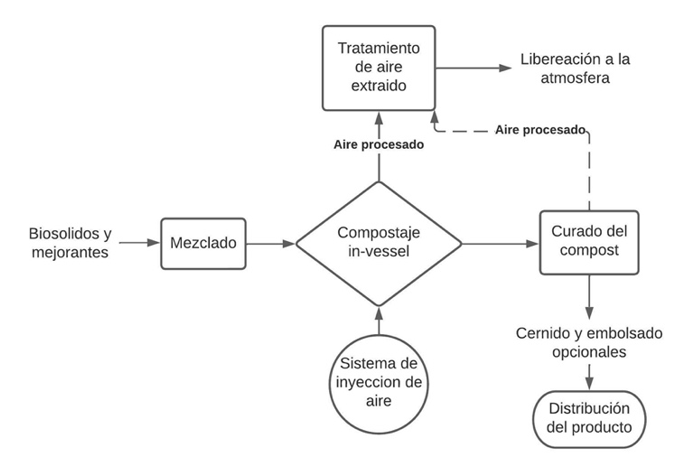
\includegraphics[scale=0.5]{images/Capitulo 1/1.2.1 Marco teorico/Proceso In vessel.png}
            \caption{Diagrama de flujo de una instalación típica de compostaje In-vessel \cite{EPA2020}}
            \label{fg:Invessel}
        \end{figure}

\subsection{Digestión aeróbica}

Consiste en la descomposición biológica de la materia orgánica en presencia de oxígeno, el cual puede ser aportado mediante agitación. Los microorganismos encargados del proceso necesitan aireación para realizar sus funciones de manera eficaz y confiable. Como consecuencia, se obtiene una reducción de olores y volumen de fangos. \cite{SULZER2015}

\subsection{Sistema de agitación}

Este sistema realizará el volteo de la materia orgánica, así como la mezcla de los materiales mientras se genera el proceso de fermentación de las sustancias biológicas. De esta manera, se busca obtener un producto homogéneo a través de los microorganismos que generan los nutrientes.

Esta tarea se puede efectuar a través de diversos tipos de herramientas, cada una adaptada a ciertas características y funciones específicas. \cite{INOX2019} (Tabla \ref{tab:agitacion})


\begin{table}
    \centering
\caption{Tipos de agitadores}
\label{tab:agitacion}
\resizebox{16cm}{!}{
    \begin{tabular}{|m{2cm}|m{5cm}|m{2cm}|m{2cm}|m{2cm}|m{2cm}|} \hline 
         Tipo&  Descripción&  Tipo de flujo&  Campo del flujo generado&  Velocidad tangencial $m/s$ & Viscosidad del medio $Pa * s$ \\ \hline 
         Palas tipo ancla&  Previene adhesión de materiaes, sus brazos llegan cerca de la pared del contenedor, su forma se puede adaptar a la estructura del tanque y favorece el intercambio de calor.&  Laminar&  Tangencial&  Máximo 2& Máximo 1000\\ \hline 
         Paletas o rejilla&  En forma de malla, trabaja a velocidades bajas en recipientes amplios y bajos. Es para fluidos viscosos, con poco esfuerzo de corte.&  Laminar&  Axial&  De 3 a 15& Menores a 8\\ \hline 
         Hélice&  Trabaja en altas velocidades, ideal para liquidos con baja viscosidad. Utilizada para homogenizar mezclas. Favorece el intercambio de calor.&  Turbulento&  Axial&  & Menores a 8\\ \hline 
         Turbina de hojas planas&  Diseño versatil y simple. El comportamiento del fluido se vuelve muy predecible. Ideal para velocidades muy bajas.&  Turbulento&  Axial&  & Menores a 0.11\\ \hline 
         Turbina de hojas inclinadas&  Las palas tienen una inclinación hacia la dirección del flujo, usualmente está comprendida de 3 palas, se utiliza para homogenizar la mezcla y mejora la transferencia de calor.&  Turbulento&  Axial&  De 3 a 8& Hasta 100\\ \hline
    \end{tabular}
    }
    
\end{table}

\subsection{Sistema de trituración}

Uno de los objetivos principales del proceso de trituración es el de reducir el tamaño de los materiales o ajustarlo a las necesidades del proyecto en el cual se utilizarán. Para ello, se requiere de maquinaria con características y funciones muy particulares. \cite{VISE}

\subsection{Sistema de Control}
La función de este sistema es la de gestionar o regular la forma en que se comporta otro sistema para así evitar un mal funcionamiento; tiene como objetivo asegurar el funcionamiento que permita cumplir con todas las tareas y asignaciones para los que fueron programados.

El sistema de control está formado por un conjunto de dispositivos de diverso orden. Pueden ser elementos eléctricos, neumáticos, hidráulicos, mecánicos, entre otros. Los tipos de elementos están determinados por la función a resolver. \cite{SCONT2020} 

Sistema de control de lazo abierto 

El control de lazo abierto se caracteriza por no incorporar un sistema de medición para evaluar el valor de salida. La regulación se hace de forma manual a partir de la experiencia o de los resultados de mediciones obtenidas previamente. \cite{SINADRIVES}

Sistema de control de lazo cerrado

El control de lazo cerrado aparece ante la necesidad de corregir de forma automática errores existentes en la salida del sistema en comparación con el valor de referencia. Esto genera la necesidad de un nuevo elemento en el sistema, un controlador. Un sensor se encarga de medir los valores a la salida, para después transmitir este valor a la entrada del sistema y, como consecuencia, modificar el sistema para obtener el valor deseado. \cite{SINADRIVES} 

\subsection{Interfaz Humano-Máquina}

Una interfaz humano-máquina (HMI por sus siglas en inglés de Human-Machine Interface) permite la comunicación entre el proceso y los operarios. Funciona como un instrumento que permite al operario manipular los procesos.

La función principal de los HMI es mostrar información sobre el monitoreo del proceso, así como ser capaz de transmitir la información operativa del equipo. También es un método por el cual se pueden controlar los objetivos del proceso.

En pocas palabras, la interfaz HMI es una herramienta que permite operar y observar las tareas que se realizan en algún dispositivo para llevar a cabo algún proceso. \cite{IHM2020}

\newpage

%%Metodología mecatrónica

\section{Marco Procedimental}

\subsection{Metodología VDI-2206}
Debido a la naturaleza de este proyecto, es necesario poder trabajarlo con una metodología que permita la integración de las diferentes disciplinas que intervienen entre sí. Es por esta razón que se ha seleccionado la metodología VDI-2206 (Figura \ref{fg}); dicha metodología posibilita afrontar el problema desde un punto de visto de diseño de ingeniería concurrente, ya que admite un desarrollo simultáneo de todos los módulos que van a comprender el sistema. Además de que es posible realizar una retroalimentación entre cada fase del proyecto. Esta metodología de modelo “V” consta de 5 pasos.(Figura \ref{fg:metodologia}).

\begin{figure}[h]
            \centering
            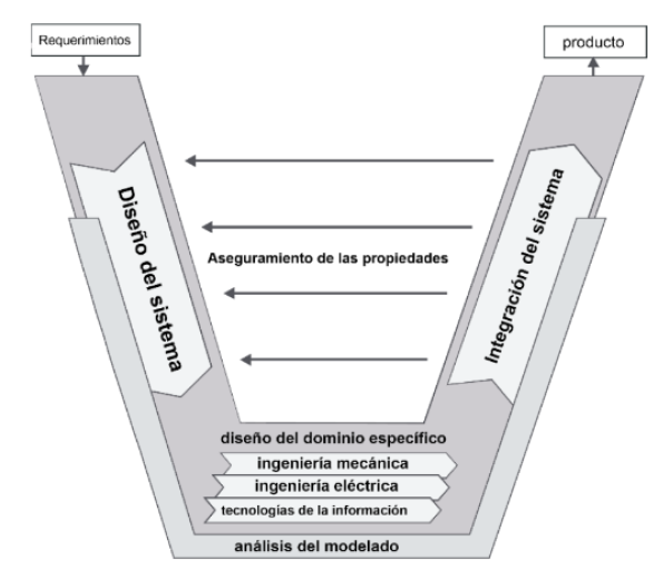
\includegraphics[scale=0.3]{images/Capitulo 1/2.2.2 Marco procedimental/VDI.png}
            \caption{Diagrama del modelo V de la metodología VDI-2206 \cite{IRI2017} }
            \label{fg:VDI}
\end{figure}



\begin{figure}[h]
            \centering
            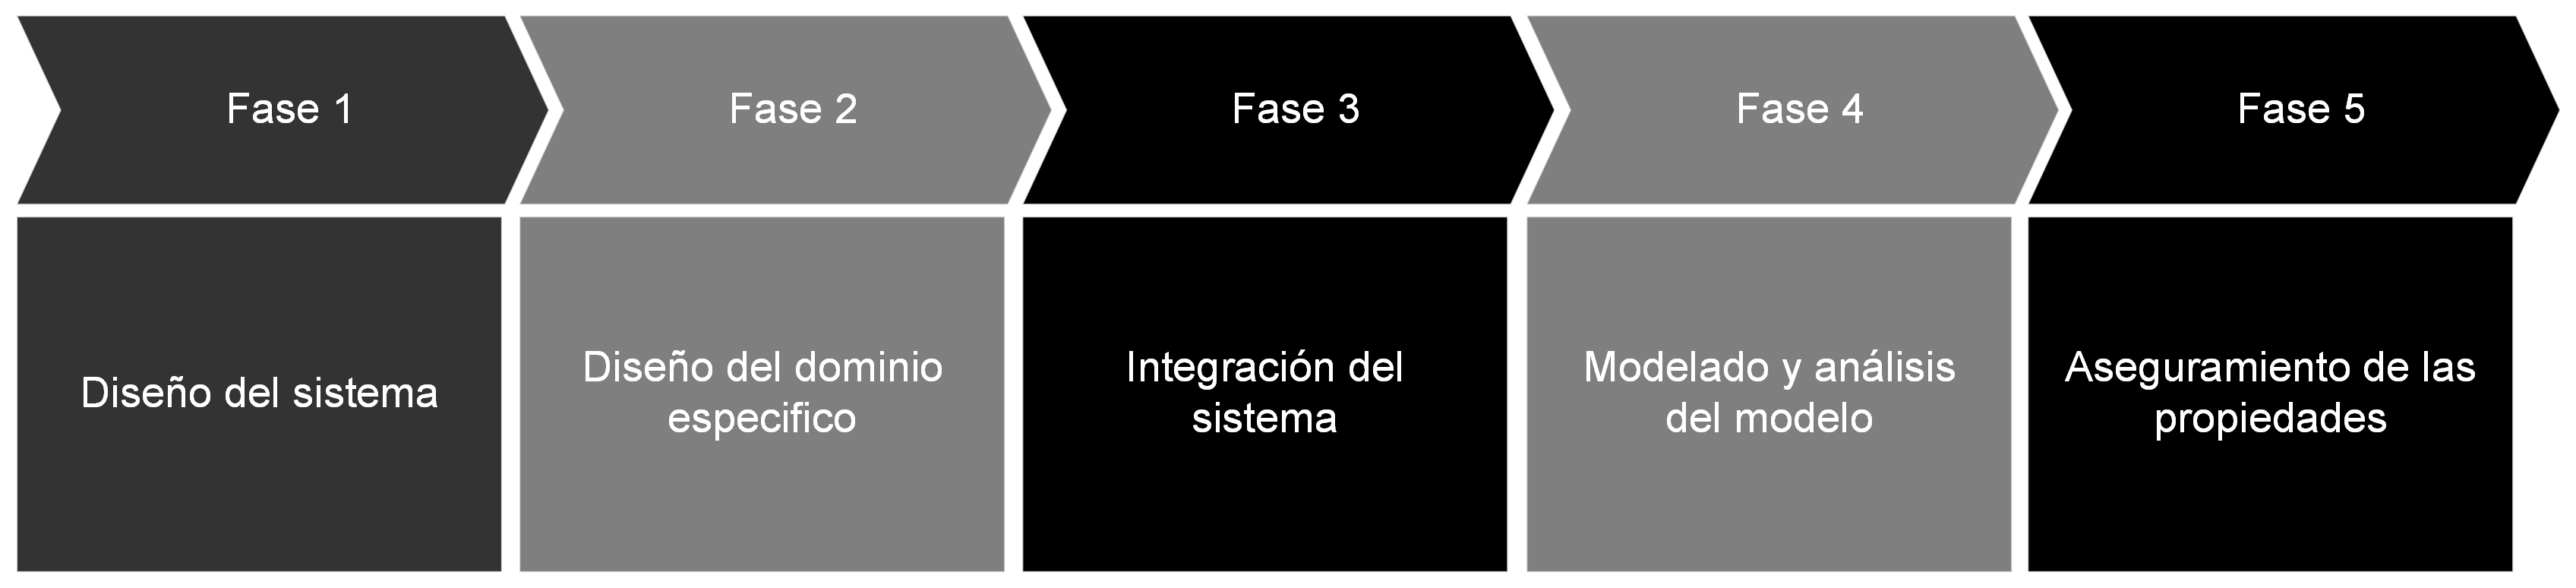
\includegraphics[scale=0.2]{images/Capitulo 1/2.2.2 Marco procedimental/Metodologia.png}
            \caption{Etapas de la metodología VDI-2206 \cite{IRI2017} }
            \label{fg:metodologia}
\end{figure}

En la primera fase, se realiza un diseño conceptual del sistema, ya que, a partir de un análisis de necesidades, se van a ir determinando los requerimientos, las funciones y la arquitectura física del sistema mecatrónico (SM). Esta etapa se ejecutará a lo largo del desarrollo de este protocolo de investigación, con el cual se sentarán las bases del proyecto. 

Es por esta razón que en esta parte del proyecto se realizarán diversos esquemas, como la Descomposición de la Estructura Funcional (FBS, por sus siglas en inglés), también el IDEF-0 para mostrar la interacción entre los módulos, que ayuden a comprender el funcionamiento general del sistema a desarrollar, en este caso, el sistema de generación de compost.




%%% modificar archivo capitulos/marcoreferencia.tex
%%%%%%%%%%%%%%%%%%%%%%%%%%capitulo1111111111%%%%%%%%%%%%%%%%\media
%\media  %%ajuste de contador de TOC %no eliminar

%\chapter{Marco de Referencia}
Esta sección del documento pretende exponer los conceptos básicos y metodologías sobre las cuales se fundamenta el proyecto que se desea desarrollar.
\section{Marco Teórico}

\subsection{Residuos orgánicos alimenticios}

En este punto se encuentra el tema central de esta investigación, el cual se trata de todos aquellos desechos orgánicos generados a partir de la preparación de los alimentos, así como los sobrantes que quedan después de ser consumidos e incluso las pérdidas que se puedan generar debido a que los productos se encuentran en estado de descomposición. \cite{CCA2017}

\subsection{Compostaje}

El compostaje es un proceso de transformación aerobia de la materia orgánica, en el cual intervienen diferentes agentes microbianos, como bacterias y hongos; siendo la razón por la que se generan ciertos fenómenos químicos, físicos y biológicos asociados con el metabolismo de estos agentes. Dichos procesos permiten acelerar la descomposición de los desechos para obtener un producto al que se le denomina compost.

Se deben tener en cuenta los diferentes factores ambientales que están relacionados de forma directa en las distintas etapas del proceso de compostaje, ya que alteran los procesos metabólicos de los microorganismos. Estos factores son la temperatura, el nivel de pH, la humedad, la cantidad de oxígeno y la relación C/N (Carbono/Nitrógeno). De esta forma, se puede obtener un desarrollo óptimo y el producto generado puede ser considerado de calidad. \cite{WIL2019}

\subsection{Tipos de procesos de compostaje}

En la actualidad existen diferentes procesos de compostaje, cada uno maneja subprocesos distintos, además de contar con herramientas y características especiales.(Tabla \ref{tab:tiposcompostaje})

\begin{table}
    \centering
\caption{Tipos de proceso de compostaje}
\label{tab:tiposcompostaje}
    \begin{tabular}{|m{2cm}|m{2cm}|m{2cm}|m{2cm}|m{2cm}|m{2cm}|} \hline 
         Tipo de proceso&  Composteras cerradas&  Takakura&  Bokashi&  Lombri - compost& Pilas\\ \hline 
         Proceso de descomposición&  Aeróbico&  Aeróbico&  Anaeróbico&  Aeróbico& Aeróbico\\ \hline 
         Producto final&  Compost&  Compost&  Pre-compost&  Humus de lombriz& Compost\\ \hline 
         Velocidad del proceso&  Rápido&  Rápido&  Rápido&  Lento& Lento\\ \hline 
         Conveniencia&  Práctico&  Medianamente práctico&  Poco Práctico&  Impráctico& Poco práctico\\ \hline 
         Generación de malor olores&  Muy baja&  Baja&  Alta &  Baja& Moderada\\ \hline 
         Residuos que procesan&  Pocas restricciones&  Algunas restricciones&  Muy pocas restricciones&  Muchas restricciones& Pocas restricciones\\ \hline 
         Inversión Inicial&  Media&  De baja a media&  De baja a media&  De media a alta& De nula a baja\\ \hline 
         Calidad del compost&  Buena&  Buena&  Bajo&  Excelente& Muy buena\\ \hline
    \end{tabular}
    
    
\end{table}

\subsection{Proceso de compostaje In Vessel}

El compostaje “In-Vessel” hace referencia al compost elaborado en un contenedor cerrado. Este tipo de contenedor ha sido utilizado en torres verticales, contenedores rectangulares y tanques circulares, así como también en tanques circulares rotatorios.

El proceso de generación de compost In-vessel (Figura \ref{fg:Invessel}) puede ser dividido en dos métodos diferentes, sistemas continuos de procesamiento, y sistemas de agitación.

En el primero, la relación de partículas de la masa de compostaje se mantiene igual durante todo el proceso y el sistema es alimentado continuamente. En los sistemas de agitación, el material de compostaje es mezclado mecánicamente de forma continua durante el proceso.

Los sistemas mecánicos están diseñados para minimizar los olores y disminuir el tiempo de procesamiento, controlando las condiciones ambientales, como lo son el flujo de aire, la temperatura y la concentración de oxígeno.

El tiempo de procesamiento en los contenedores cerrados varía de una a dos semanas, pero comúnmente los sistemas emplean de cuatro a doce semanas de estabilización después del periodo activo. \cite{ONU2020}

\begin{figure}[ht]
            \centering
            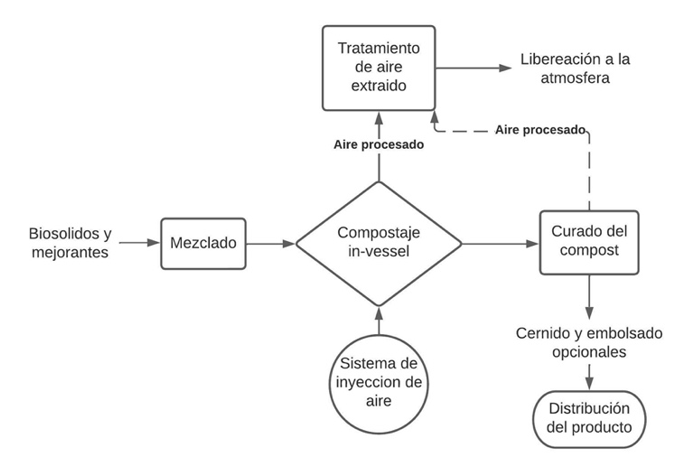
\includegraphics[scale=0.5]{images/Capitulo 1/1.2.1 Marco teorico/Proceso In vessel.png}
            \caption{Diagrama de flujo de una instalación típica de compostaje In-vessel \cite{EPA2020}}
            \label{fg:Invessel}
        \end{figure}

\subsection{Digestión aeróbica}

Consiste en la descomposición biológica de la materia orgánica en presencia de oxígeno, el cual puede ser aportado mediante agitación. Los microorganismos encargados del proceso necesitan aireación para realizar sus funciones de manera eficaz y confiable. Como consecuencia, se obtiene una reducción de olores y volumen de fangos. \cite{SULZER2015}

\subsection{Sistema de agitación}

Este sistema realizará el volteo de la materia orgánica, así como la mezcla de los materiales mientras se genera el proceso de fermentación de las sustancias biológicas. De esta manera, se busca obtener un producto homogéneo a través de los microorganismos que generan los nutrientes.

Esta tarea se puede efectuar a través de diversos tipos de herramientas, cada una adaptada a ciertas características y funciones específicas. \cite{INOX2019} (Tabla \ref{tab:agitacion})


\begin{table}
    \centering
\caption{Tipos de agitadores}
\label{tab:agitacion}
\resizebox{16cm}{!}{
    \begin{tabular}{|m{2cm}|m{5cm}|m{2cm}|m{2cm}|m{2cm}|m{2cm}|} \hline 
         Tipo&  Descripción&  Tipo de flujo&  Campo del flujo generado&  Velocidad tangencial $m/s$ & Viscosidad del medio $Pa * s$ \\ \hline 
         Palas tipo ancla&  Previene adhesión de materiaes, sus brazos llegan cerca de la pared del contenedor, su forma se puede adaptar a la estructura del tanque y favorece el intercambio de calor.&  Laminar&  Tangencial&  Máximo 2& Máximo 1000\\ \hline 
         Paletas o rejilla&  En forma de malla, trabaja a velocidades bajas en recipientes amplios y bajos. Es para fluidos viscosos, con poco esfuerzo de corte.&  Laminar&  Axial&  De 3 a 15& Menores a 8\\ \hline 
         Hélice&  Trabaja en altas velocidades, ideal para liquidos con baja viscosidad. Utilizada para homogenizar mezclas. Favorece el intercambio de calor.&  Turbulento&  Axial&  & Menores a 8\\ \hline 
         Turbina de hojas planas&  Diseño versatil y simple. El comportamiento del fluido se vuelve muy predecible. Ideal para velocidades muy bajas.&  Turbulento&  Axial&  & Menores a 0.11\\ \hline 
         Turbina de hojas inclinadas&  Las palas tienen una inclinación hacia la dirección del flujo, usualmente está comprendida de 3 palas, se utiliza para homogenizar la mezcla y mejora la transferencia de calor.&  Turbulento&  Axial&  De 3 a 8& Hasta 100\\ \hline
    \end{tabular}
    }
    
\end{table}

\subsection{Sistema de trituración}

Uno de los objetivos principales del proceso de trituración es el de reducir el tamaño de los materiales o ajustarlo a las necesidades del proyecto en el cual se utilizarán. Para ello, se requiere de maquinaria con características y funciones muy particulares. \cite{VISE}

\subsection{Sistema de Control}
La función de este sistema es la de gestionar o regular la forma en que se comporta otro sistema para así evitar un mal funcionamiento; tiene como objetivo asegurar el funcionamiento que permita cumplir con todas las tareas y asignaciones para los que fueron programados.

El sistema de control está formado por un conjunto de dispositivos de diverso orden. Pueden ser elementos eléctricos, neumáticos, hidráulicos, mecánicos, entre otros. Los tipos de elementos están determinados por la función a resolver. \cite{SCONT2020} 

Sistema de control de lazo abierto 

El control de lazo abierto se caracteriza por no incorporar un sistema de medición para evaluar el valor de salida. La regulación se hace de forma manual a partir de la experiencia o de los resultados de mediciones obtenidas previamente. \cite{SINADRIVES}

Sistema de control de lazo cerrado

El control de lazo cerrado aparece ante la necesidad de corregir de forma automática errores existentes en la salida del sistema en comparación con el valor de referencia. Esto genera la necesidad de un nuevo elemento en el sistema, un controlador. Un sensor se encarga de medir los valores a la salida, para después transmitir este valor a la entrada del sistema y, como consecuencia, modificar el sistema para obtener el valor deseado. \cite{SINADRIVES} 

\subsection{Interfaz Humano-Máquina}

Una interfaz humano-máquina (HMI por sus siglas en inglés de Human-Machine Interface) permite la comunicación entre el proceso y los operarios. Funciona como un instrumento que permite al operario manipular los procesos.

La función principal de los HMI es mostrar información sobre el monitoreo del proceso, así como ser capaz de transmitir la información operativa del equipo. También es un método por el cual se pueden controlar los objetivos del proceso.

En pocas palabras, la interfaz HMI es una herramienta que permite operar y observar las tareas que se realizan en algún dispositivo para llevar a cabo algún proceso. \cite{IHM2020}

\newpage

%%Metodología mecatrónica

\section{Marco Procedimental}

\subsection{Metodología VDI-2206}
Debido a la naturaleza de este proyecto, es necesario poder trabajarlo con una metodología que permita la integración de las diferentes disciplinas que intervienen entre sí. Es por esta razón que se ha seleccionado la metodología VDI-2206 (Figura \ref{fg}); dicha metodología posibilita afrontar el problema desde un punto de visto de diseño de ingeniería concurrente, ya que admite un desarrollo simultáneo de todos los módulos que van a comprender el sistema. Además de que es posible realizar una retroalimentación entre cada fase del proyecto. Esta metodología de modelo “V” consta de 5 pasos.(Figura \ref{fg:metodologia}).

\begin{figure}[h]
            \centering
            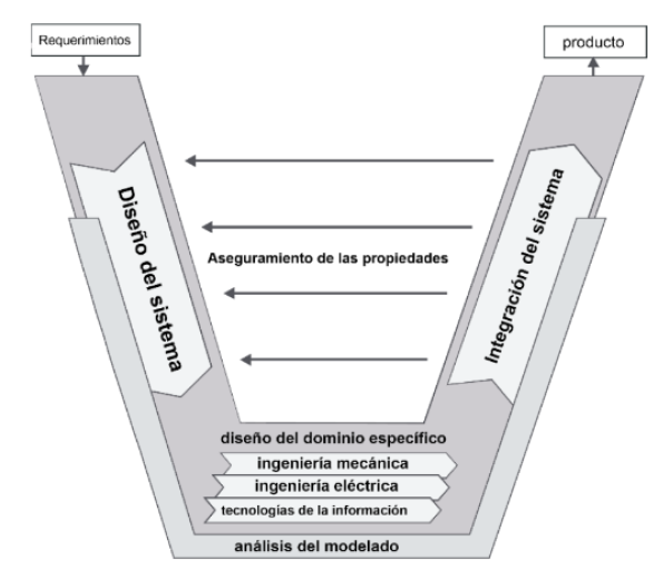
\includegraphics[scale=0.3]{images/Capitulo 1/2.2.2 Marco procedimental/VDI.png}
            \caption{Diagrama del modelo V de la metodología VDI-2206 \cite{IRI2017} }
            \label{fg:VDI}
\end{figure}



\begin{figure}[h]
            \centering
            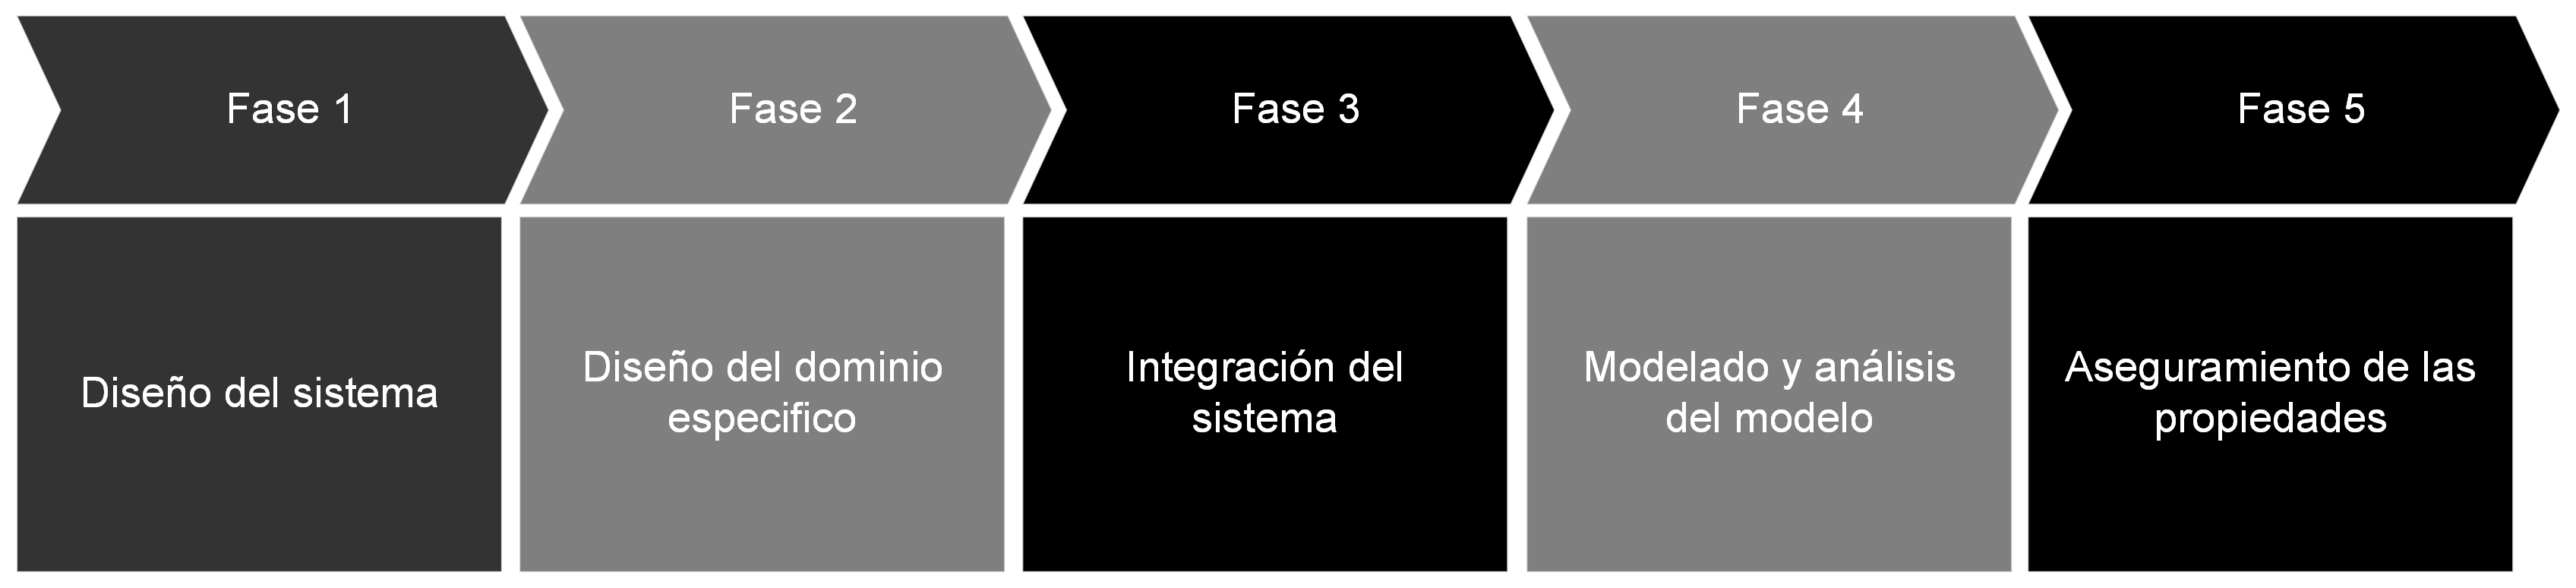
\includegraphics[scale=0.2]{images/Capitulo 1/2.2.2 Marco procedimental/Metodologia.png}
            \caption{Etapas de la metodología VDI-2206 \cite{IRI2017} }
            \label{fg:metodologia}
\end{figure}

En la primera fase, se realiza un diseño conceptual del sistema, ya que, a partir de un análisis de necesidades, se van a ir determinando los requerimientos, las funciones y la arquitectura física del sistema mecatrónico (SM). Esta etapa se ejecutará a lo largo del desarrollo de este protocolo de investigación, con el cual se sentarán las bases del proyecto. 

Es por esta razón que en esta parte del proyecto se realizarán diversos esquemas, como la Descomposición de la Estructura Funcional (FBS, por sus siglas en inglés), también el IDEF-0 para mostrar la interacción entre los módulos, que ayuden a comprender el funcionamiento general del sistema a desarrollar, en este caso, el sistema de generación de compost.



%%%modificar archivo capitulos/marcoreferencia.tex
%%%%%%%%%%%%%%%%%%%%%%%%%%%%%%%%%%%%%%%%%%%%%%%%%%%%%%%%%%%%%%%%%%%
%%%%%%%%%%%%%%%%%%%%%%%%%%%%%%%%%%%%%%%%%%%%%%%%%%%%%%%%%%%%%%%%%%%

\chapter{Diseño del sistema}

\section{Diseño Conceptual}

\subsection{Necesidades y requerimientos}

Para el desarrollo del proyecto, es muy importante identificar cada una de las necesidades que se pueden encontrar al momento de realizar el planteamiento del problema. Estas necesidades están sintetizadas en la tabla \ref{tab:Necesidades}. 

\begin{table}[h]
  \centering
  \begin{tabular}{|c|c|c|}
    \hline
    No. & Necesidad & Clasificación \\
    \hline
    N1 & Procesar residuos orgánicos & Funcional \\
    N2 & Controlar temperatura & Funcional \\
    N3 & Controlar humedad & Funcional \\
    N4 & Producir una mezcla homogénea con los residuos ingresados & Funcional \\
    N5 & Disminuir el tamaño de los residuos & Funcional \\
    N6 & Capacidad de almacenamiento & Funcional \\
    N7 & Aislamiento térmico & Funcional \\
    N8 & Estabilidad estructural & No Funcional \\
    N9 & Monitorización de producto & Funcional \\
    N10 & Filtrar malos olores & Funcional \\
    N11 & Durabilidad del producto & No Funcional \\
    \hline
  \end{tabular}
  \caption{Necesidades}
  \label{tab:Necesidades}
\end{table}


Los requerimientos nacen de las necesidades funcionales del sistema y estos deben de ser medibles y alcanzables para asegurar el funcionamiento del proyecto. Es de esta forma que se pueden establecer los siguientes requerimientos mostrados en la tabla \ref{tab:requerimientos}.
\clearpage
    
\begin{table}
  \centering
  \begin{tabularx}{\linewidth}{|c|X|c|c|c|c|}
    \hline
    \# & Descripción & NF & F & Importancia & Valor \\
    \hline
    R1 & Duración del ciclo de procesamiento &  & X & 5 & 72 horas \\ \hline
    R2 & Triturar residuos Vegetales y Frutales & & X & 5 & dureza < 10 HB \\ \hline
    R3 & Realizar el control de temperatura de acuerdo con las fases del proceso & & X & 5 & \makecell{ -Fase Mesófila I: 25-45 $^oC$  \\ -Fase Termofila: 45-60 $^oC$ \\ -Fase Mesófila II: 45-30 $^oC$ } \\ \hline
    R4 & Realizar el control de humedad & & X & 5 & 40-60 $\%$ \\ \hline
    R5 & Velocidad angular del eje de aireación & & X & 5 & 4-6 rpm \\ \hline
    R6 & Tamaño del residuo antes del triturado & & X & 4 & 30-50 mm \\ \hline
    R7 & Tamaño del residuo después del triturado & X & & 4 & 3-4 mm \\ \hline
    R8 & Volumen del contenedor & & X & 4 & 120 L \\ \hline
    R9 & Masa total de residuos a procesar por ciclo & X & & 4 & 8-15 kg \\ \hline
    R10 & Reducción de la perdida de calor & & X & 3 & \makecell{ Conductividad térmica \\ < 51.9 W/mK} \\ \hline
    R11 & Estabilidad Estructural & X & & 5 & Factor de Seguridad > 8 \\ \hline
    R12 & Envío de mediciones a base de datos & & X & 2 & 2 veces por minuto\\ \hline
    R13 & Área de trabajo & & X & 2 & 1.5 m$^2$ \\
    \hline
  \end{tabularx}
  \caption{Requerimientos}
  \label{tab:requerimientos}
\end{table}

\clearpage

De las tablas anteriores se detectó que debe tener componentes de alta fiabilidad, ya que funcionará continuamente durante una gran cantidad de tiempo, y materiales de baja fiabilidad podrían llevar al mal funcionamiento del sistema.

\newpage



\subsection{Funcionamiento general}

 %% Texto del cuerpo del documento
 En la ilustración \ref{fg:diagflujo}, se muestra un diagrama de flujo, el cual busca simplificar el funcionamiento general del sistema de compostaje, enlazando cada uno de los módulos y cómo será su orden dentro del proceso de compostaje. 

%% Insertar una imagen 
        \begin{figure}[h!]
            \centering
            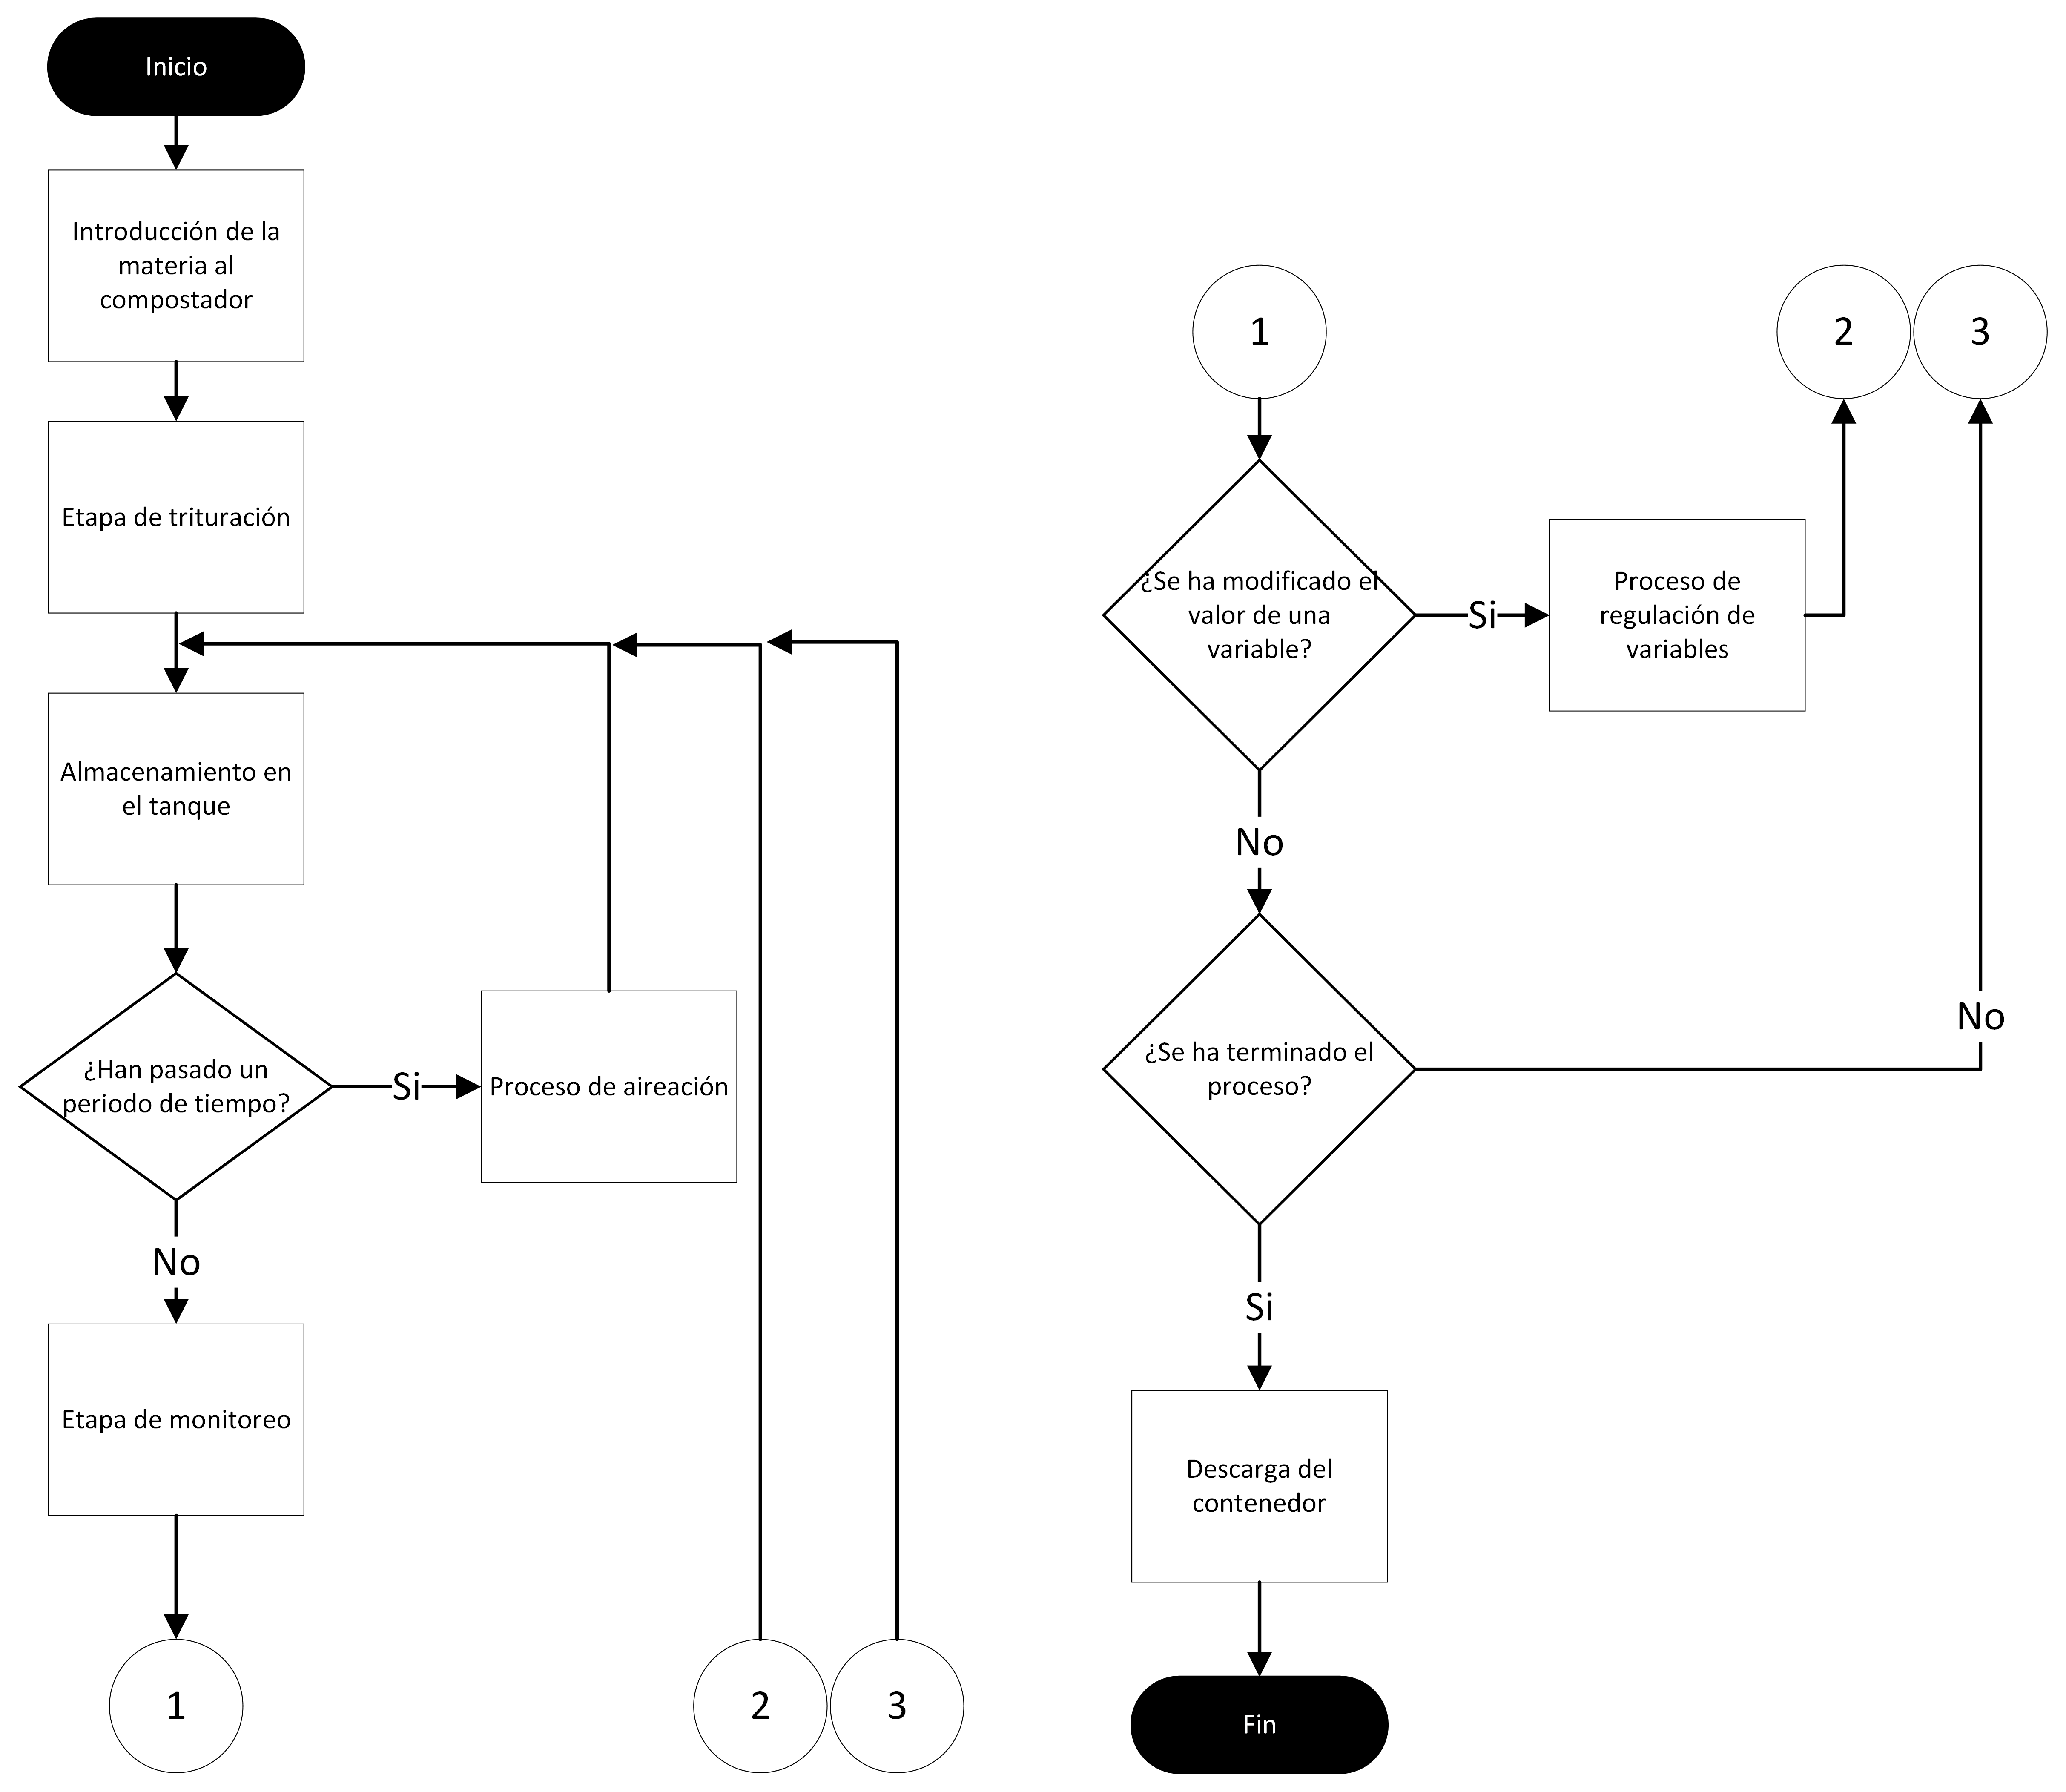
\includegraphics[scale=0.25]{images/Capitulo 3/Presentacion del proceso/Diagrama de flujo del sistema.png}
            \caption{Diagrama de flujo del funcionamiento general del sistema}
            \label{fg:diagflujo}
        \end{figure}
        
 El primer módulo que se presenta corresponde a la “Introducción de la materia al compostador”. Esta carga de materia se hace de forma manual, vertiendo la materia orgánica por un conducto especial que va enlazado a la etapa de trituración.
 
Se plantea que la etapa de trituración sea ejecutada de forma manual, de manera que sea el esfuerzo del usuario el que realice el movimiento del sistema de trituración con ayuda de un sistema mecánico de transmisión de movimiento.

La etapa de almacenamiento hace referencia al espacio donde se va a realizar el proceso de compostaje, ya que el método In-Vessel requiere de un contenedor dentro del cual se pueda adaptar el ambiente necesario para el crecimiento de microorganismos.

Dentro del recipiente de almacenaje, se realizará la etapa de control, a partir de una subetapa de monitoreo y una regulación. Con ayuda de diversos sensores, se busca monitorear el estado de las variables y, si es necesario, con ayuda de diversos actuadores, se busca regularlas dentro de unos parámetros determinados de forma automática.

Otro proceso en paralelo es la etapa de agitación. Esta etapa se encarga de mover la materia orgánica; es un proceso necesario para oxigenar a los microorganismos y lograr la homogeneización del compost. Este proceso se realiza cada cierto periodo de tiempo de forma automática.

Por último, la etapa de descarga del compost se hará a través de una de las laterales del contenedor. Esta etapa se realiza de manera manual.

\subsection{Arquitectura funcional}
De acuerdo con los requerimientos definidos en la etapa anterior, se pueden enumerar las funciones necesarias los procesos del sistema. Estas se pueden dividir en varias subfunciones para visualizar mejor cada uno de los procesos que se llevarán a cabo dentro del dispositivo. Estas funciones se pueden ver de forma jerárquica en la figura \ref{fg:Funciones} y también es posible observar su interrelación en el diagrama IDEF-0 que se muestra en la figura \ref{fg:IDEFGeneral}. Con mayor detalle, puede revisar el apéndice \ref{Ap:IDEF0}.

0. Función Principal: \textbf{Generar compost }
\begin{itemize}
    \item 1. Recepción de la materia
    \begin{itemize}
        \item 1.1 Triturar la materia a la entrada
        \item 1.2 Conducir la materia al interior del contenedor
        \begin{itemize}
            \item 1.2.1. Empujar la materia al interior
            \item 1.2.2. Almacenar la materia
        \end{itemize}
    \end{itemize}
    \item 2. Regular las diferentes etapas del proceso de compostaje
    \begin{itemize}
        \item 2.1. Gestionar el periodo de tiempo para cada fase
        \begin{itemize}
            \item 2.1.1. Contar horas, minutos y segundos.
            \item 2.1.2 Delimitar cada periodo de inicio y final en cada etapa del proceso.
        \end{itemize}
        \item 2.2. Regular la temperatura en cada fase de manera automática.
        \begin{itemize}
            \item 2.2.1 Monitorear el valor de la temperatura
            \item 2.2.2 En caso de una temperatura inferior, encender los actuadores necesarios para incrementar la temperatura de la materia.
            \item 2.2.3 En caso de una temperatura superior, encender los actuadores necesarios para disminuir la temperatura
            \item 2.2.4 Conservar una temperatura constante al interior del contenedor.
            \begin{itemize}
                \item 2.2.4.1 Reducir las pérdidas de calor.
                \item 2.2.4.2 Contar con un cierre firme para evitar las fugas de materia orgánica.
            \end{itemize}
        \end{itemize}
    \end{itemize}
    \item 3. Gestionar los tiempos del proceso de aireación
    \begin{itemize}
        \item 3.1. Contar el tiempo para activar cada ciclo de aireación.
        \item 3.2. Activar de manera automática cada uno de los actuadores para el proceso de aireación.
    \end{itemize}
    \item 4. Gestionar la comunicación con el usuario
    \begin{itemize}
        \item 4.1. Mantener una comunicación bidireccional por medio de una interfaz humano-maquina
        \begin{itemize}
            \item 4.1.1. Enviar información del proceso
            \begin{itemize}
                \item 4.1.1.1. Enviar información sobre el ambiente al interior del contenedor
                \item 4.1.1.2. Enviar información sobre que proceso se esta ejecutando
                \item 4.1.1.3. Enviar información sobre el tiempo total del proceso.
            \end{itemize}
            \item 4.1.2. Recibir indicaciones para activar los diferentes actuadores un modo de prueba.
        \end{itemize}
        \item 4.2. Mantener una comunicación unidireccional a través de un sitio web.
        \begin{itemize}
            \item 4.2.1 Enviar información sobre las variables ambientales al interior del contenedor
            \item 4.2.2. Enviar información sobre que actuadores están activos.
            \item 4.2.3. Enviar información sobre el tiempo total del proceso.
        \end{itemize}
    \end{itemize}
\end{itemize}

\begin{figure}[h!]
            \centering
            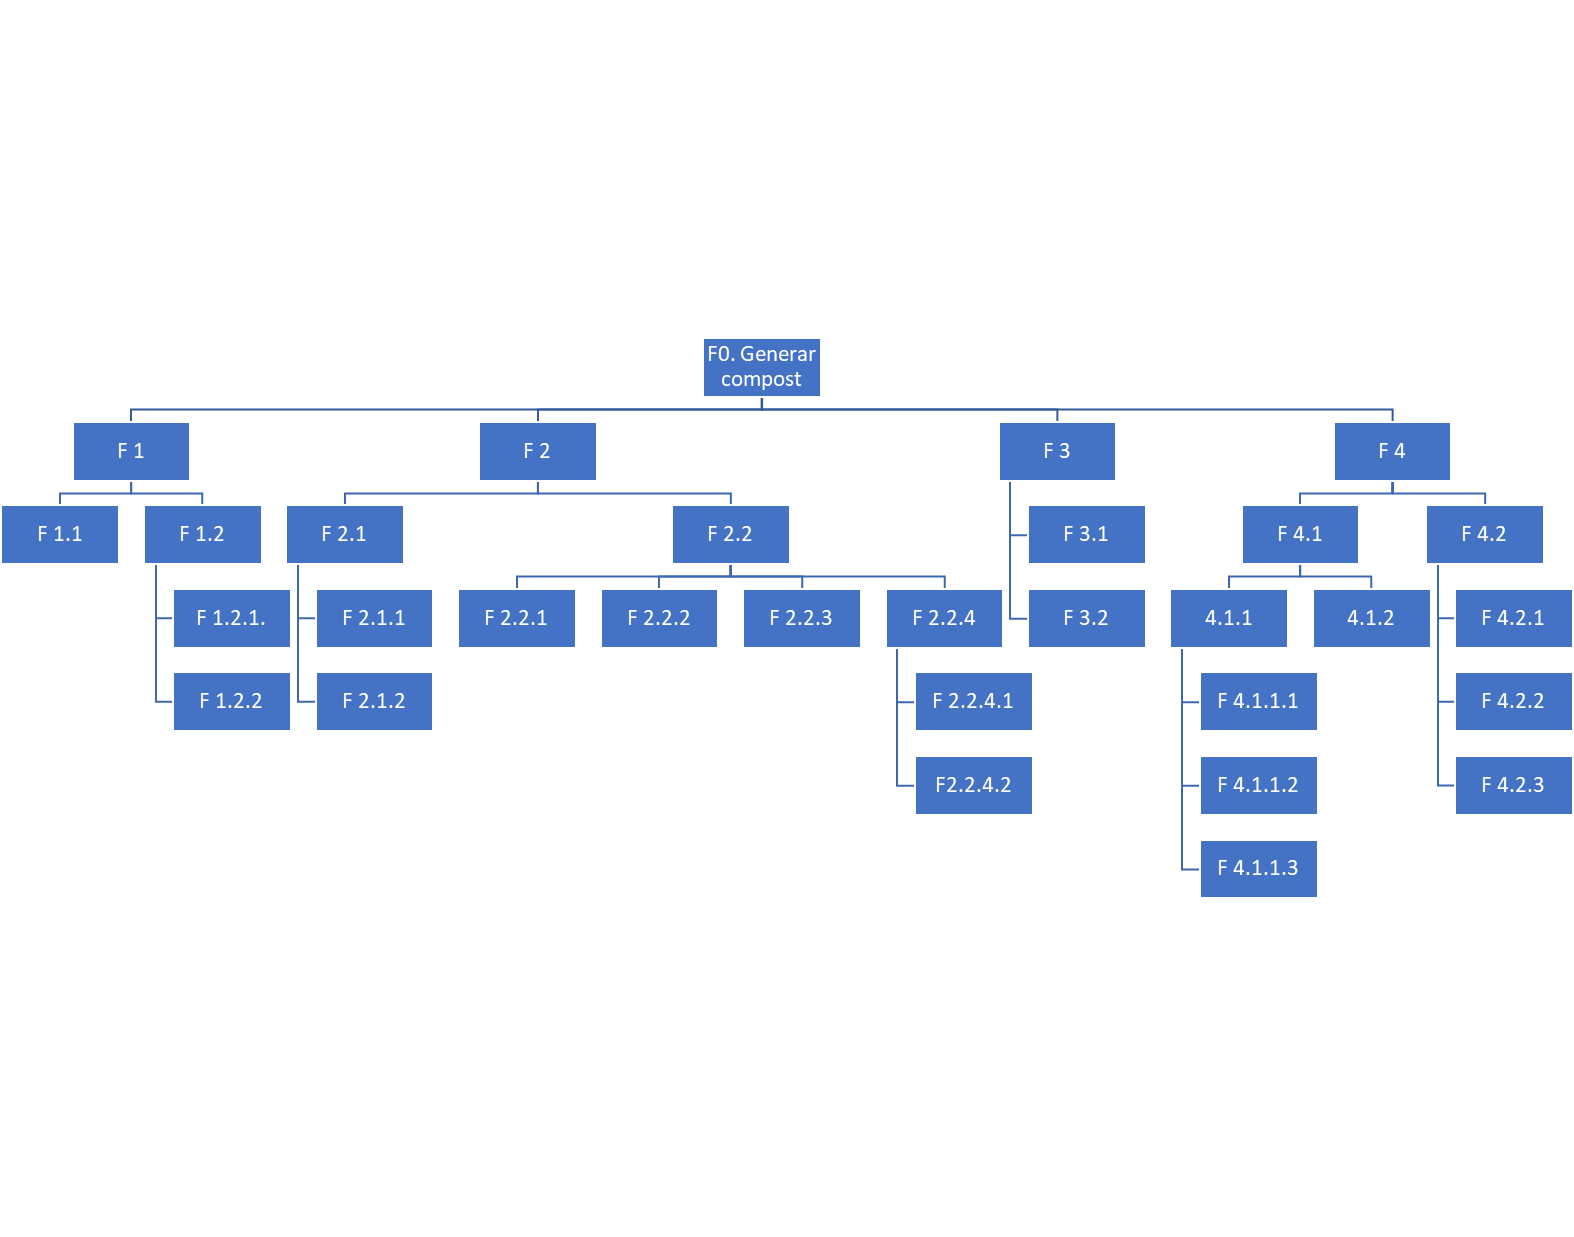
\includegraphics[scale=0.3, angle = 90]{images/Capitulo 3/3.1.1.2 Arquitectura funcional/FBS2.png}
            \caption{Diagrama FBS del sistema}
            \label{fg:Funciones}
        \end{figure}

\newpage

\begin{figure}[h!]
            \centering
            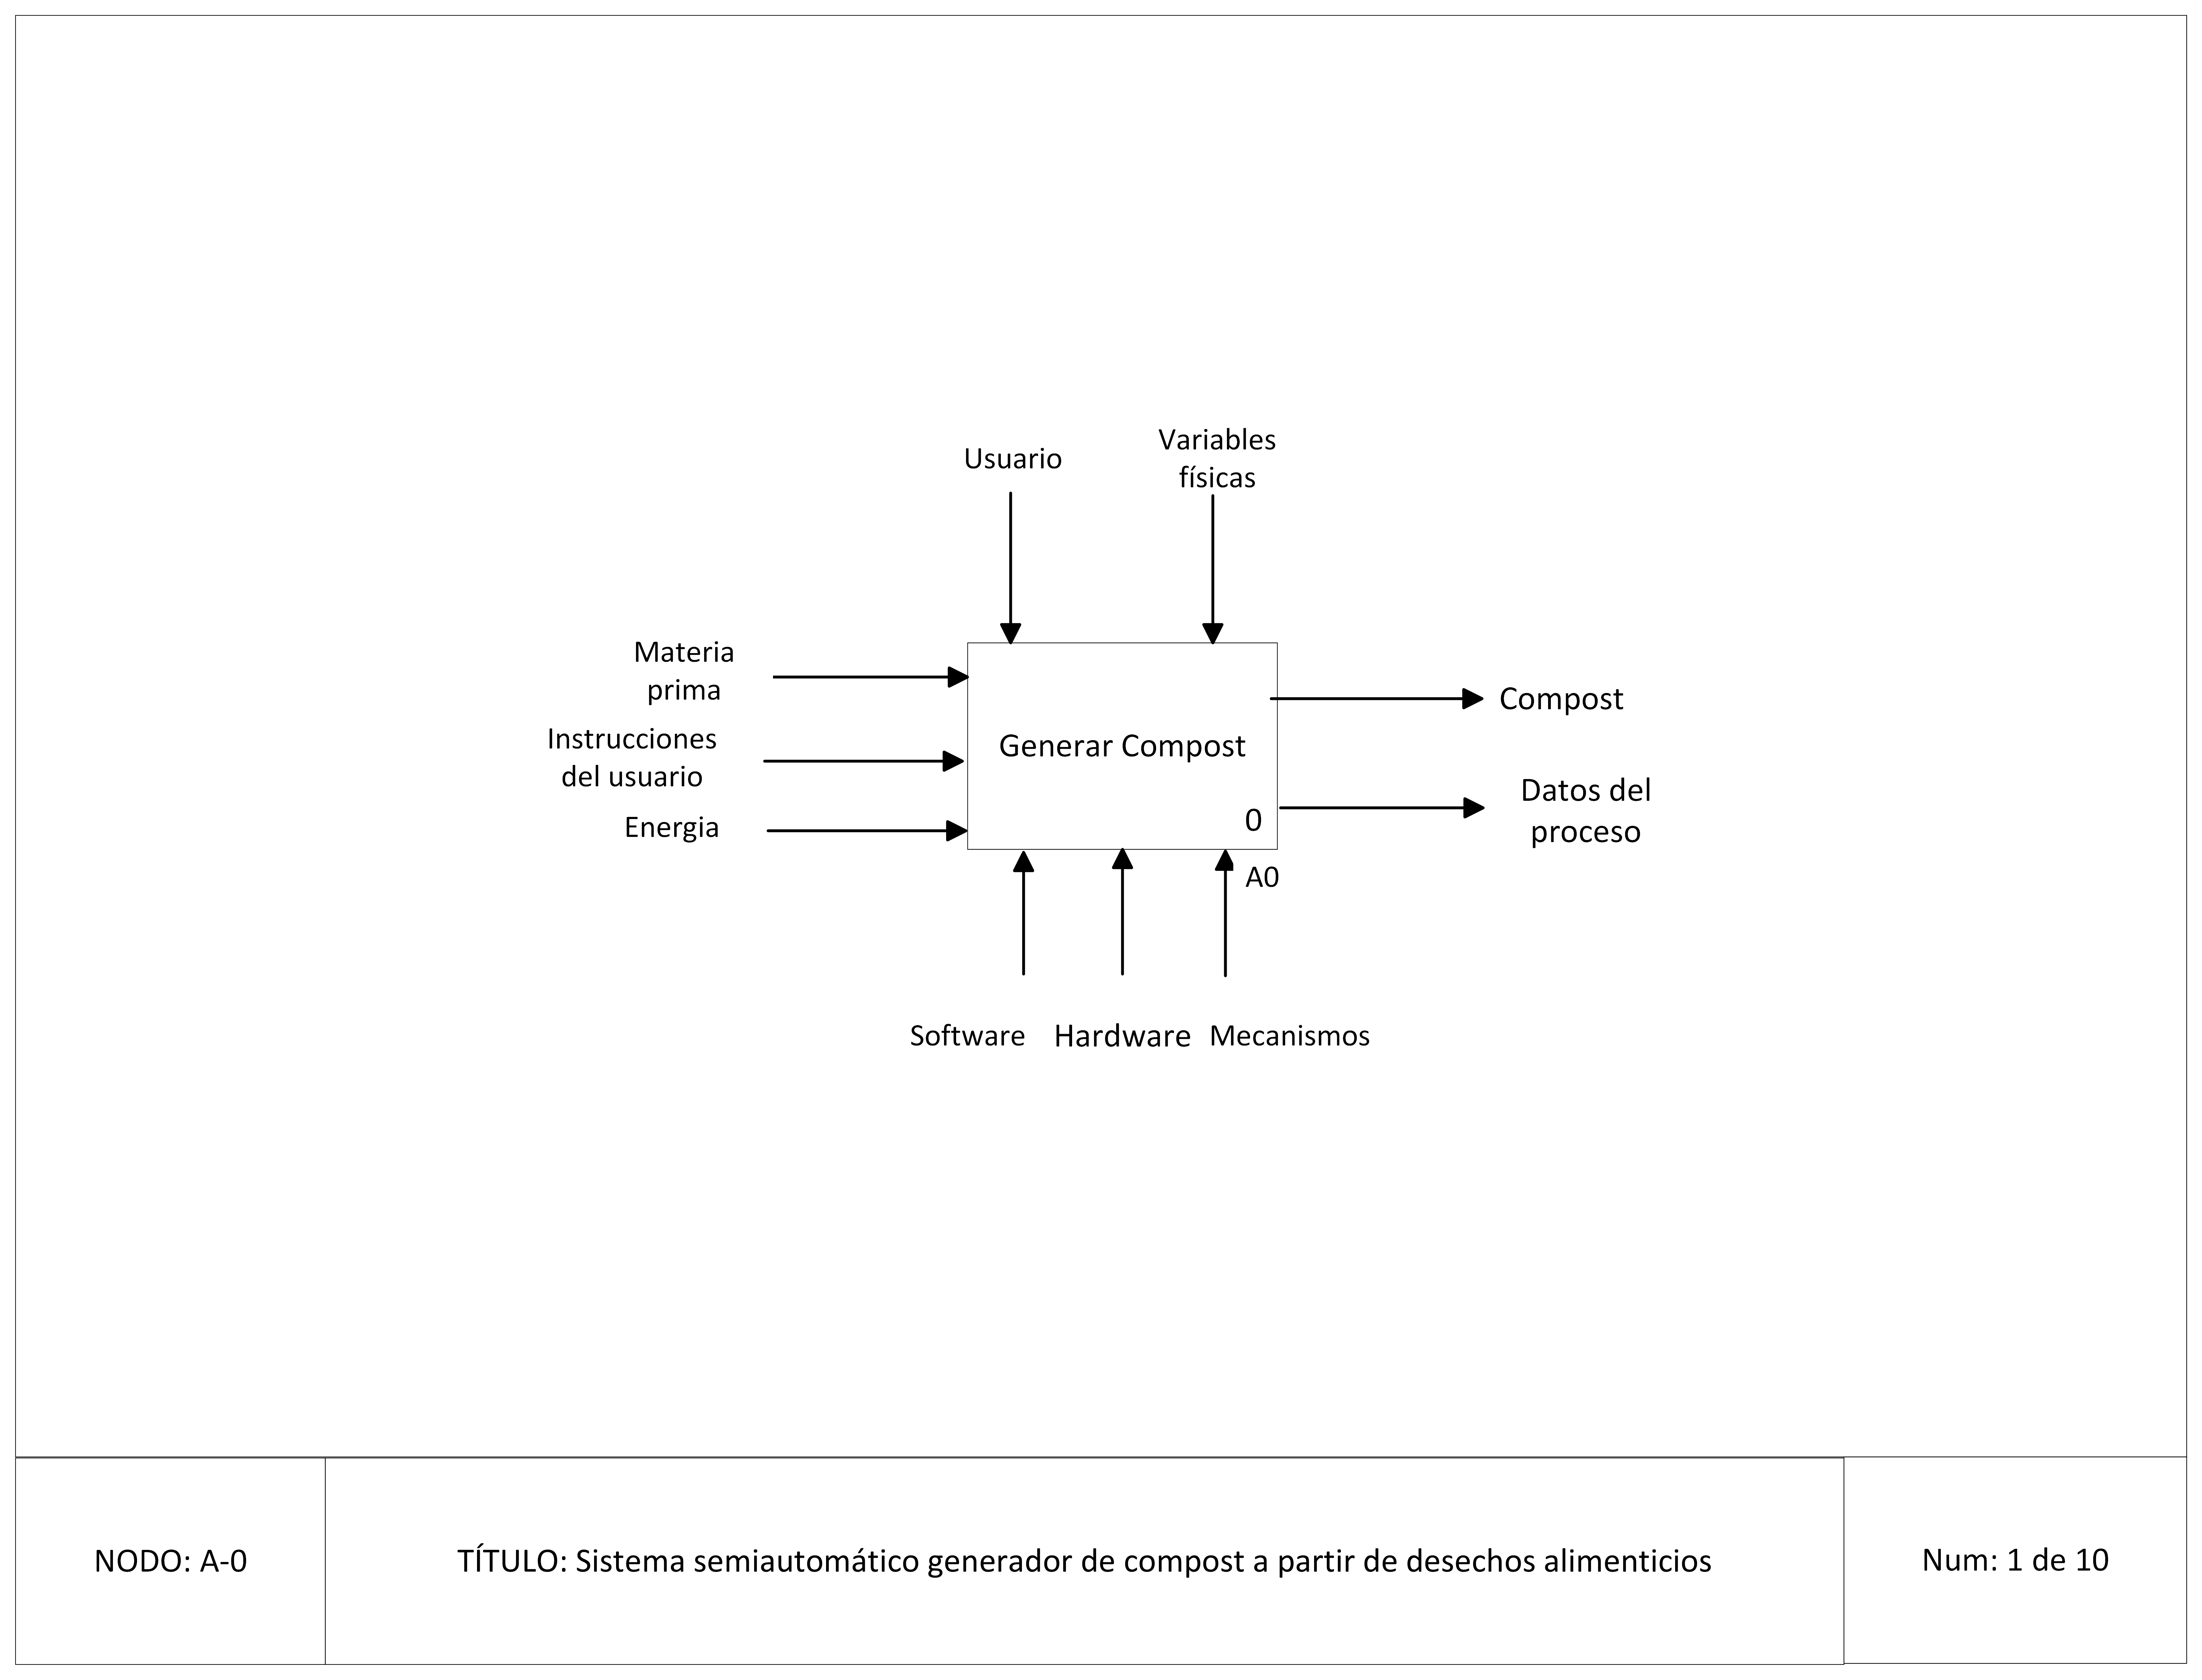
\includegraphics[scale=0.2, angle = 90]{images/Capitulo 6 Apéndices/01 IDEF 0/General.png}
            \caption{IDEF0 del sistema}
            \label{fg:IDEFGeneral}
\end{figure}

\newpage        
Una vez que se han descrito las entradas y las salidas requeridas del sistema, es necesario detallar cómo es que se interrelacionan las diferentes funciones en su interior. En la figura \ref{fg:IDEFA0} se presenta el Nodo: A0 expandido, mostrando de forma detallada la función \textbf{Generación de compost}.

\begin{figure}[h!]
    \centering
    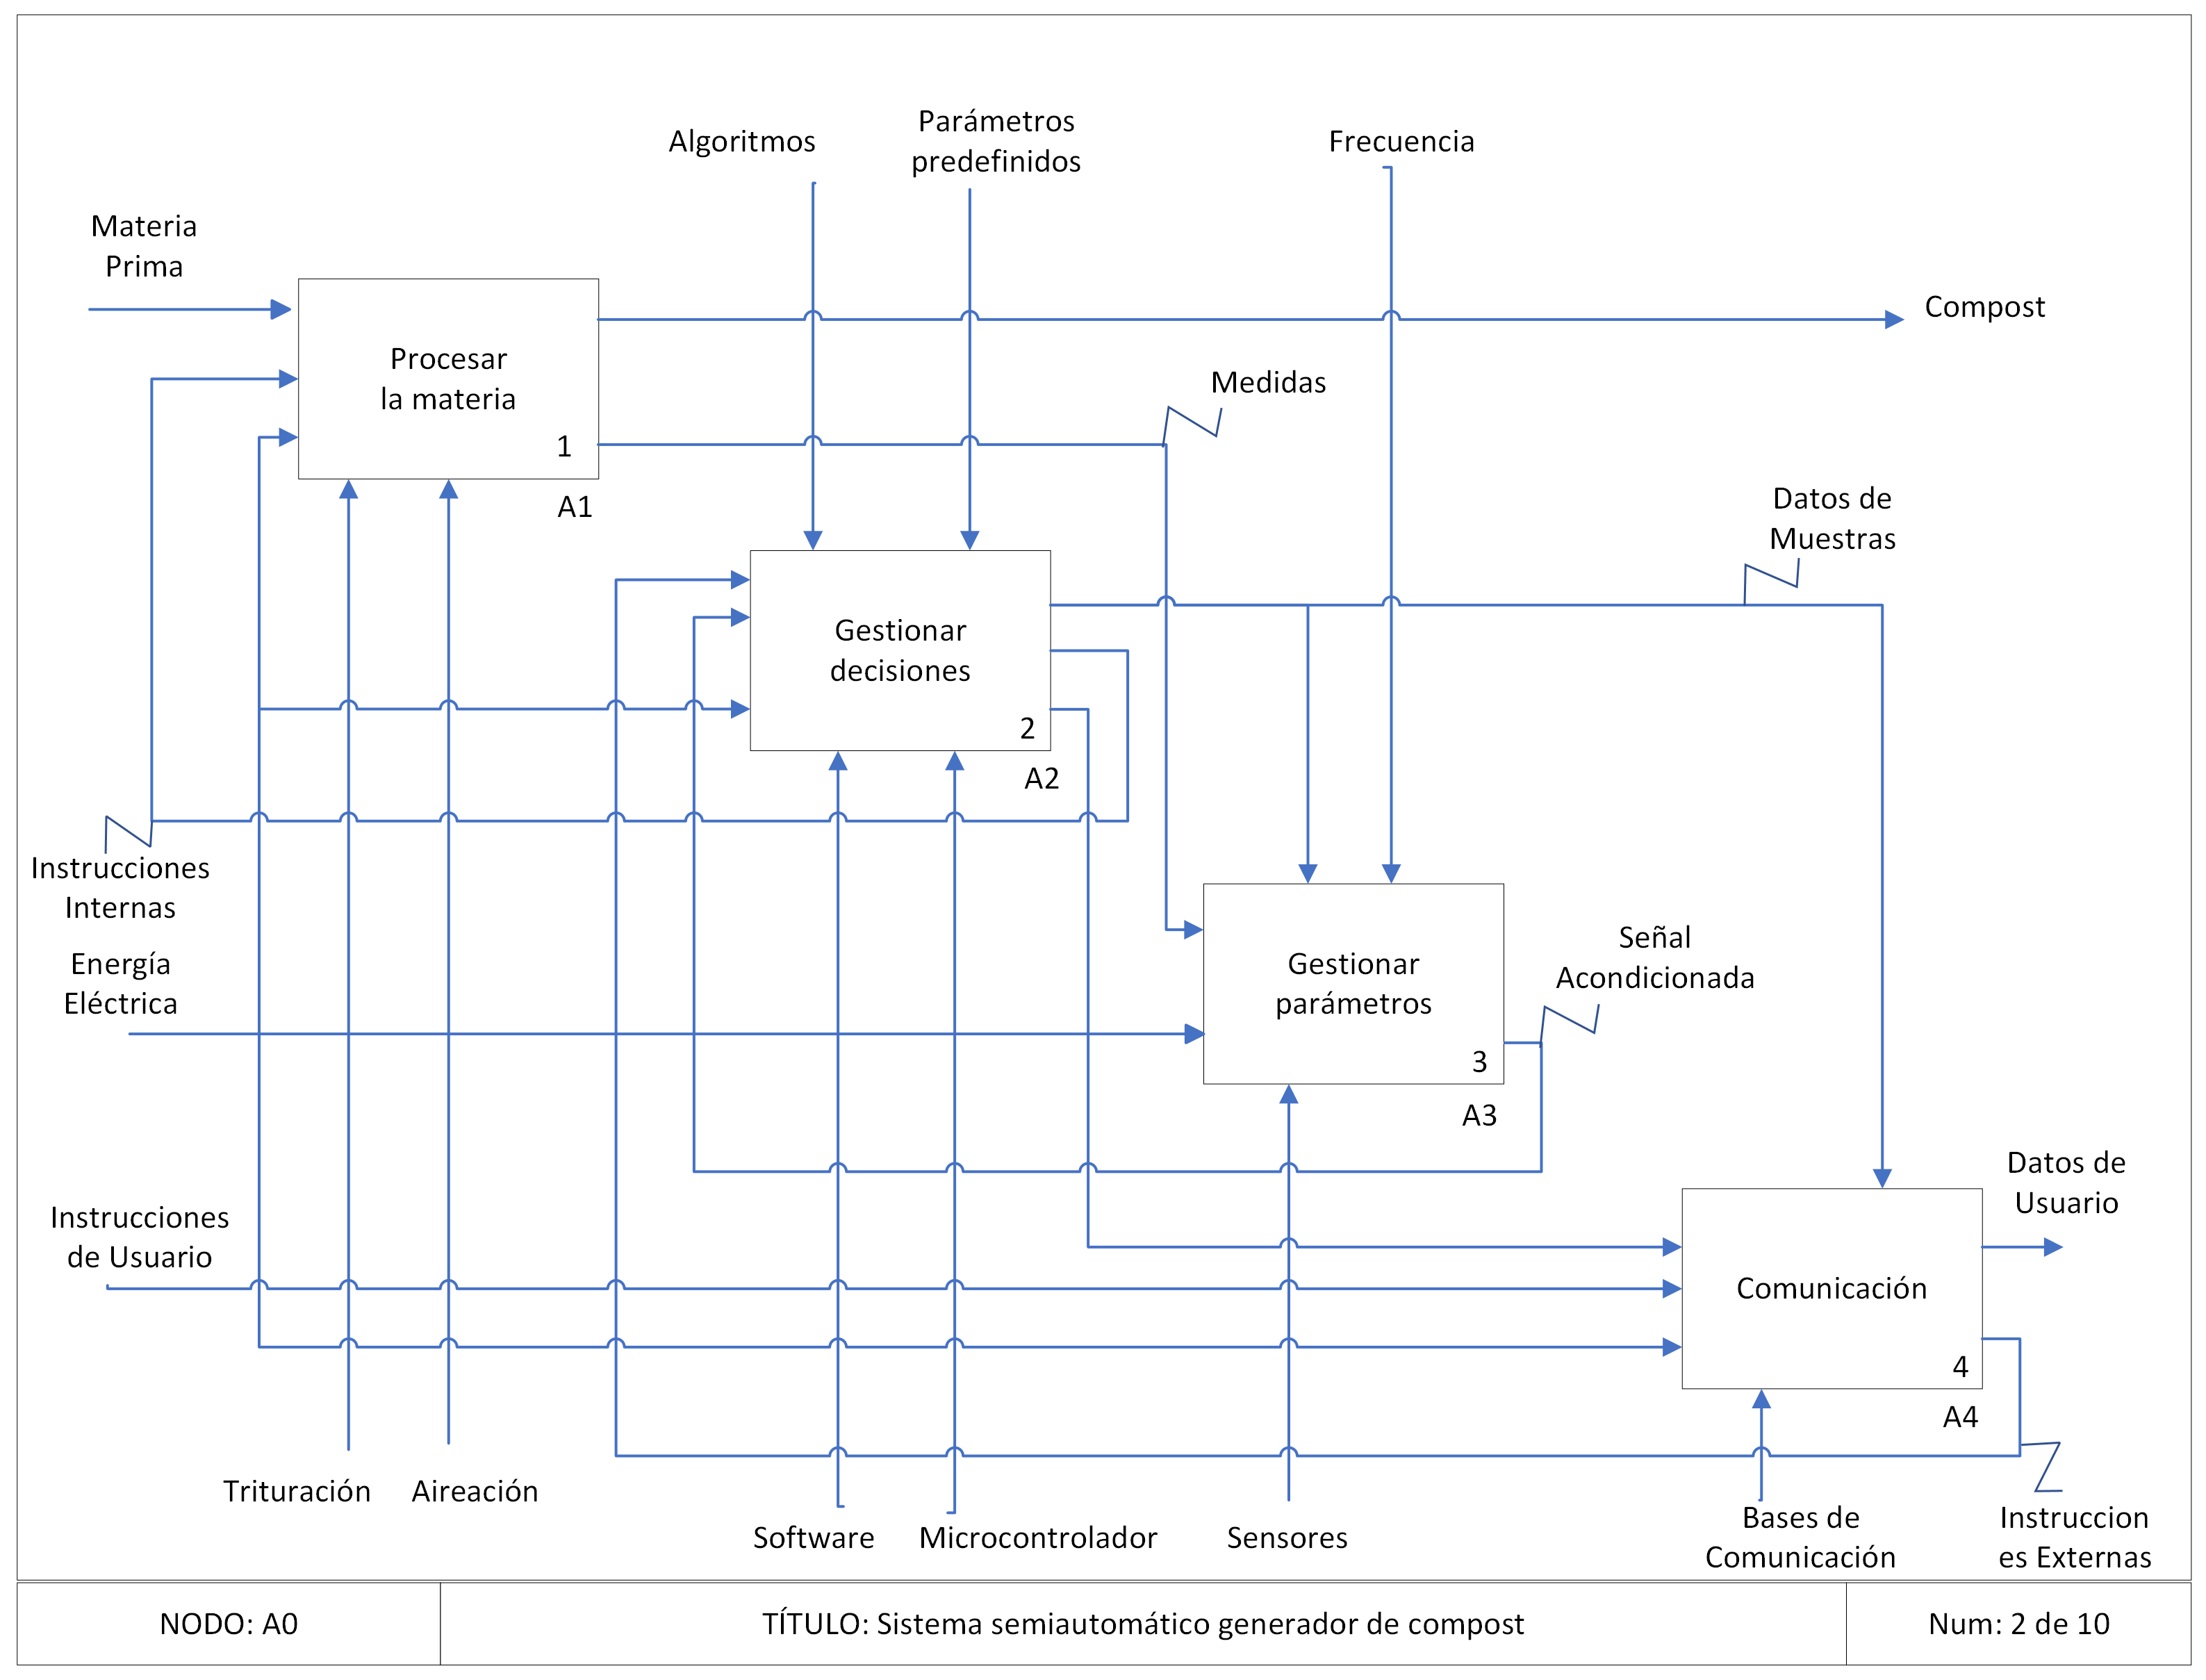
\includegraphics[scale=0.2, angle = 90]{images/Capitulo 6 Apéndices/01 IDEF 0/NodoA0.png}
    \caption{IDEF0 Nodo: A0}
    \label{fg:IDEFA0}
\end{figure}

De esta forma, se puede observar cómo se describen las funciones principales del sistema, a partir de las entradas principales: \textbf{Materias primas}, \textbf{Instrucciones del usuario} y \textbf{Energía eléctrica}. 

El sistema será capaz de proveer a la salida \textbf{Compost}, además de entregar \textbf{Datos al usuario} sobre el estado de las variables físicas internas del dispositivo e información sobre el proceso de compostaje. Para poder obtener las salidas deseadas del sistema, es necesario que los procesos y las funciones principales estén controladas por diversas herramientas, como lo son \textbf{Algoritmos de programación}, \textbf{Los parámetros predefinidos}, \textbf{Instrucciones de usuario}, así como \textbf{Señales de comunicación internas} las cuales son necesarias para coordinar la operaciones y las etapas de cada uno de los procesos requeridos para generar el ambiente que beneficie los procesos de descomposición. 




\subsection{Arquitectura física}
Después de haber realizado el análisis del funcionamiento del sistema a partir de la división de la función principal en varias subfunciones y de conocer la interrelación que existe en cada una de ellas, es posible agruparlas en diferentes módulos y sistemas. 

Para lograr dicho cometido, se utilizará el SPA (System Physical Architecture), que es la representación de la transformación de funciones en sistemas, subsistemas, ensambles y componentes físicos. \cite{Flores2018} Estos sistemas deben estar ligados a las funciones del dominio funcional y cumplir con los requerimientos del sistema para asegurar el correcto funcionamiento del prototipo.

Para plantear el modelo, se parte de una arquitectura genérica para sistemas mecatrónicos, que servirá como referencia para la construcción de la arquitectura física del sistema. (Figura \ref{fg:ArchFis})

\textbf{Sistema de administración de comportamiento $(S_1)$}: Este sistema se encargará de la toma de decisiones del sistema, a través de un módulo de análisis de información $(M_{11})$, el cual se encarga de analizar los datos obtenidos del sistema $(S_2)$; a su vez tomará las decisiones $(M_{12})$ para regular las acciones de cada sistema. 

\textbf{Sistema de procesamiento de datos $(S_2)$}: Este sistema se encargará de adquirir los datos internos y externos que son necesarios para controlar el sistema. Cuenta con un módulo para adquirir datos$(M_{21})$ que se obtienen a través de sensores colocados en el sistema $(S_5)$ y también de la interfaz Humano-Máquina del sistema $S_6$, al mismo tiempo estos datos pasan por la etapa de Acondicionamiento de señales $(M_{22})$, el cual prepara los datos para poder ser trabajados en el sistema $S_1$. Este último contará con un módulo de Comunicación $(M_{23})$ el cual se encargará de transmitir las señales procesadas a todos los sistemas que lo requieran. También se cuenta con un Módulo de Interfaz Humano-Máquina $(M_{24})$, que sirve para la interacción del usuario con el sistema mecatrónico.

\textbf{Sistema de energía $(S_3)$}: Este sistema se encargará de la administración de la energía eléctrica dentro del dispositivo. Primero pasa por un Módulo de transformación $(M_{31})$, que es el encargado de transformar la energía, ya sea regulación de AC o transformándola en DC, según se requiera en el dispositivo. Pasa al módulo encargado de Regular la tensión $(M_{32})$ para los dispositivos electrónicos de los sistemas $S_1$ y $S_2$, así como transmitir la energía necesaria para la alimentación de los motores $(M_{33})$ para los sistemas $S_4$ y $S_5$.

\textbf{Sistema de trituración de residuos $(S_4)$}: Este sistema se encargará de reducir el tamaño de los residuos suministrados.

\textbf{Sistema de procesamiento $(S_5)$}: Este es el sistema donde se llevará a cabo la mayor parte del proceso de compostaje, empezando por el módulo de aireación $(M_{51})$ el cual se encargará de mezclar los residuos y de permitir la oxigenación de la mezcla; a su vez, contará con el módulo de autorregulación $(M_{52})$ el cual recibe los datos gestionados del $S_1$ y realiza los procesos para regular el ambiente del proceso.

%\textbf{Sistema de Comunicación Externa}: Este sistema cuenta el modulo de Recepción de instrucciones $(M_{61})$ el cual se encarga de recibir las instrucciones del usuario y también cuenta con un modulo de Comunicación de datos $(M_{62})$ el cual muestra los datos sobre el proceso y las variables del ambiente al usuario. 

La interconexión de los diferentes módulos del dispositivo se puede observar en la figura \ref{fg:ArchFis}

\begin{figure}[h!]
            \centering
            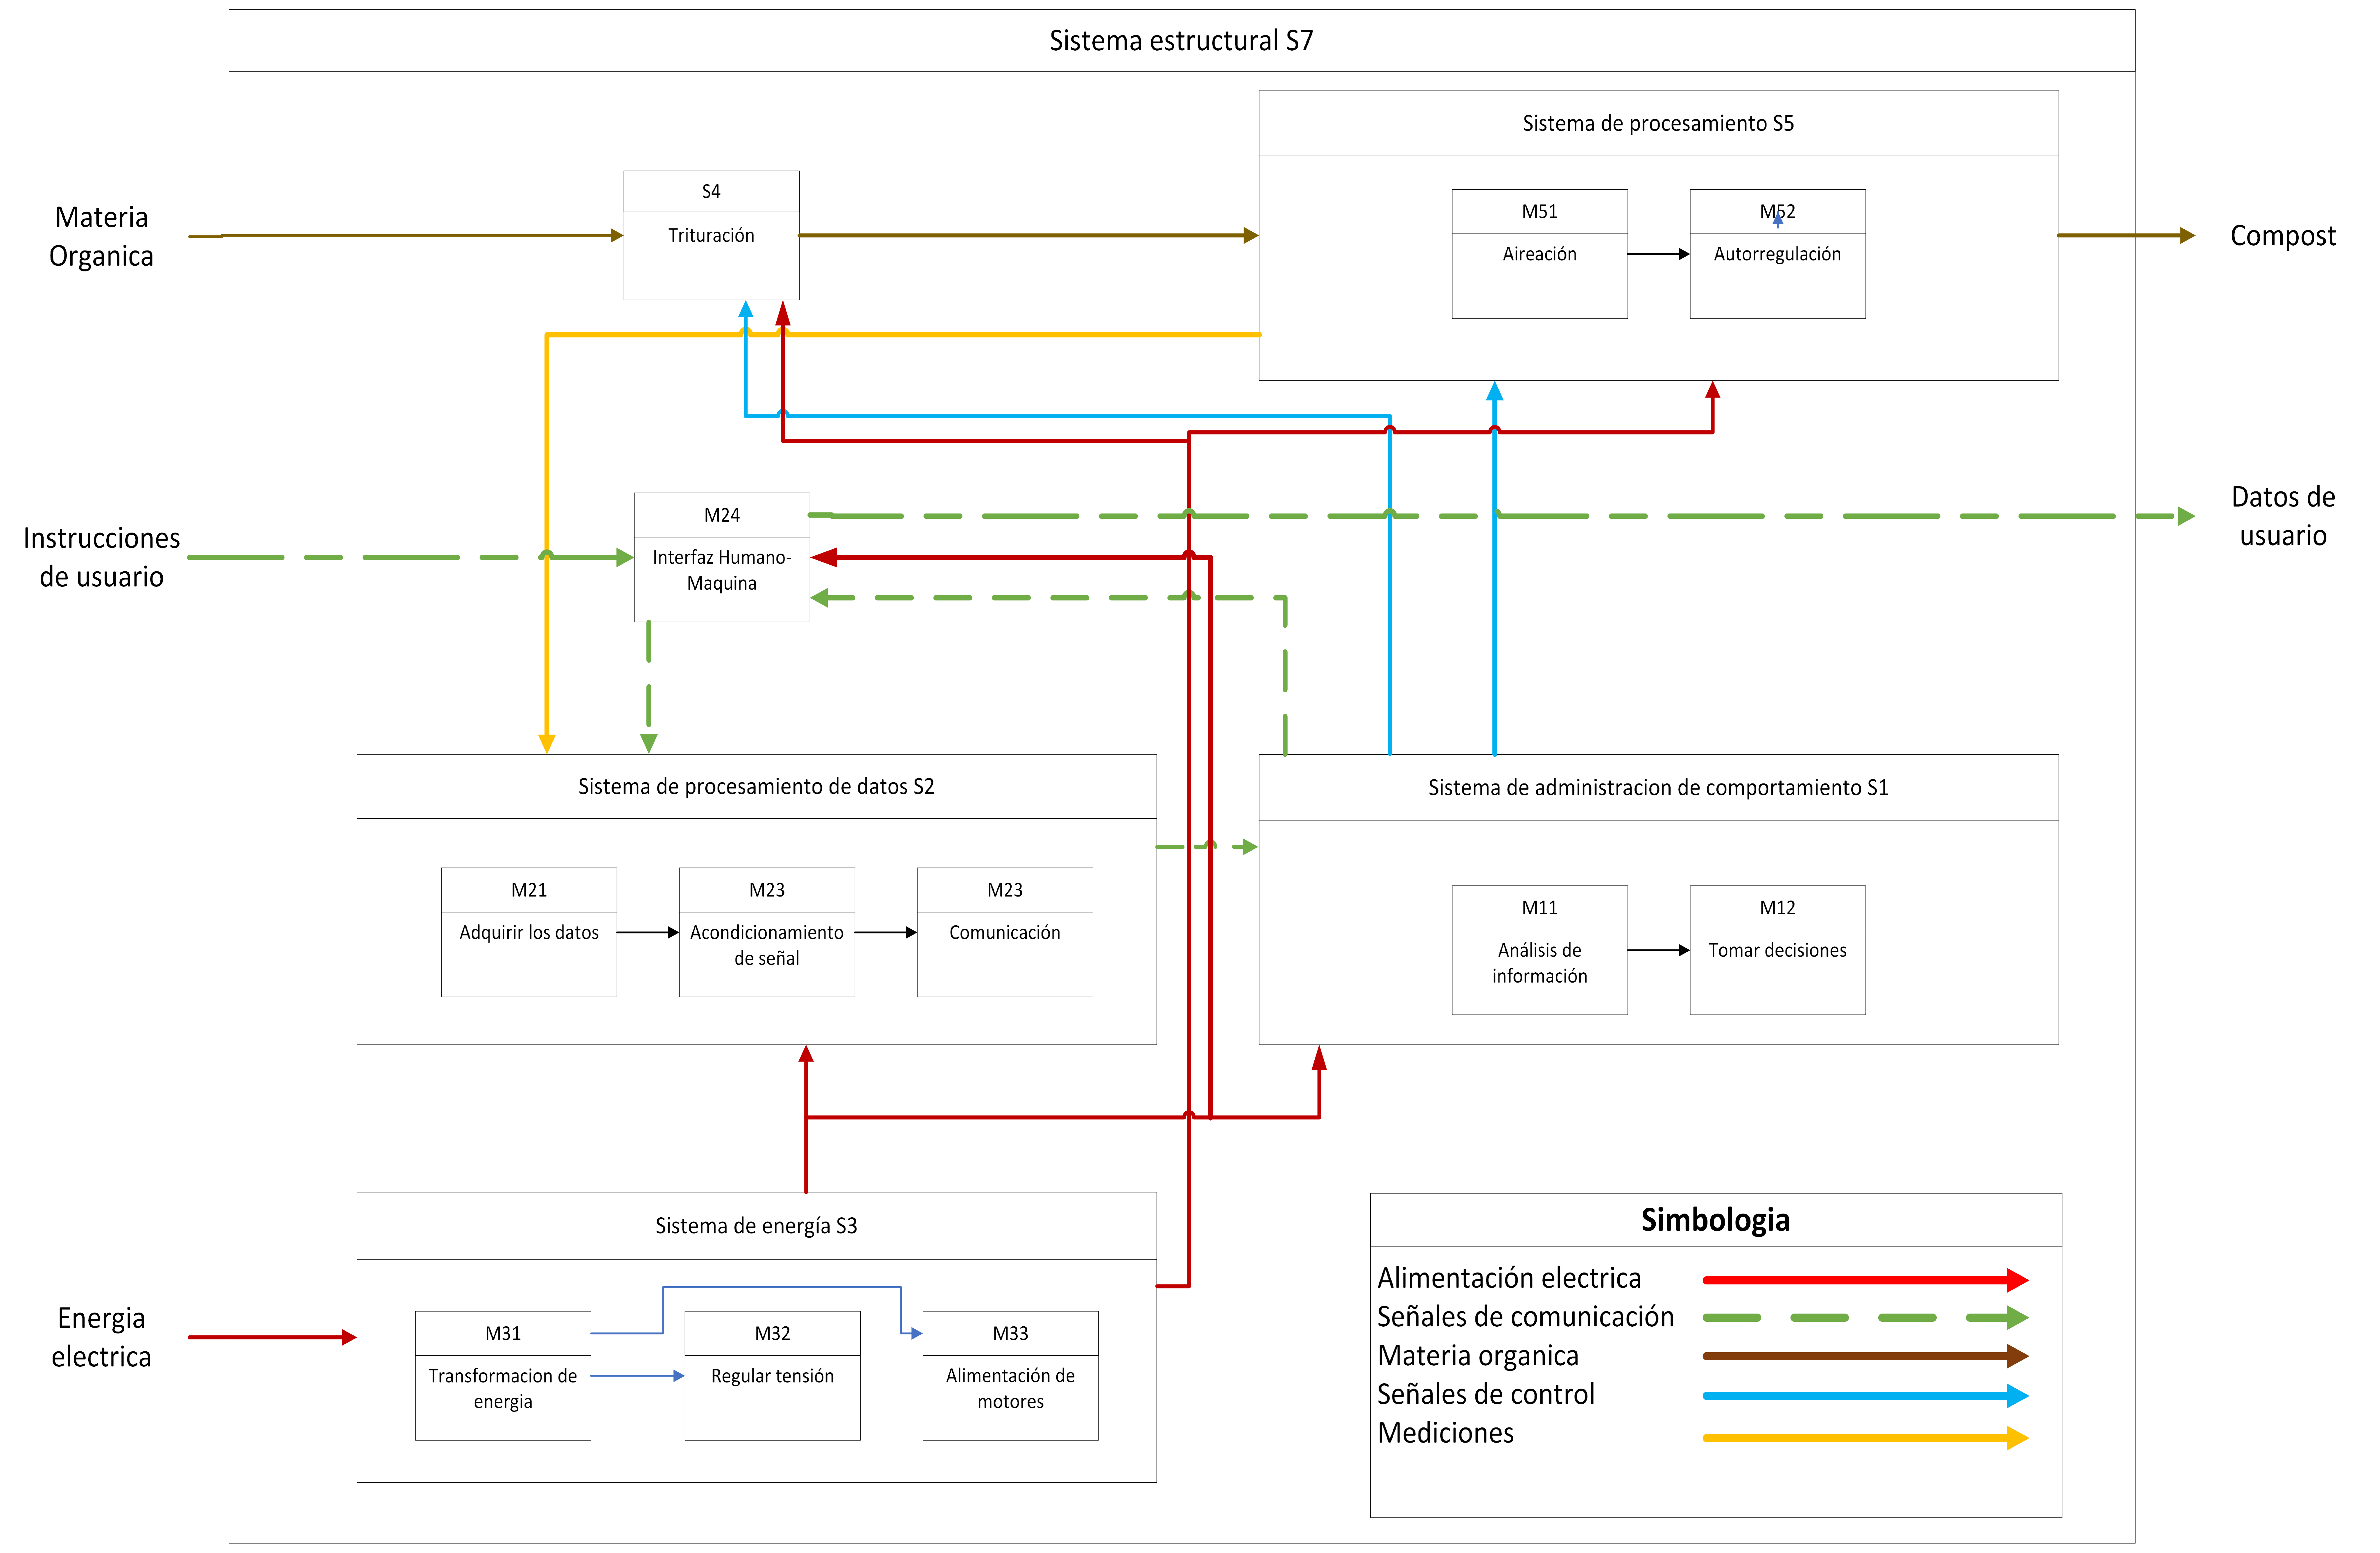
\includegraphics[scale=0.2, angle = 90]{images/Capitulo 3/3.1.1.3 Arquitectura fisica/Arquitectura fisica.png}
            \caption{Arquitectura física propuesta}
            \label{fg:ArchFis}
        \end{figure}

\newpage

\subsection{Propuesta solución}

Para la concepción de la propuesta solución, fue necesario realizar un análisis por medio de una matriz morfológica. Esta es una tabla en la que se ilustran las diferentes opciones que se pueden seleccionar para la construcción de los diferentes sistemas del dispositivo. 

Dentro de ella se trazan diversas rutas de diseño a través de las cuales se van seleccionando los mecanismos necesarios y se va dando forma a un diseño conceptual del dispositivo mecatrónico.

Para este proyecto, se propone la matriz morfológica que se encuentra en el apéndice \ref{Ap:Mat_Morfo}, donde se muestran las opciones que existen para construir los diferentes sistemas de trituración, aireación, monitoreo, regulación y comunicación.
        
De esta forma, se comienzan a trazar diferentes rutas de diseño en la tabla morfológica para seleccionar cada una de las partes del diseño del sistema y así proponer diferentes modelos del sistema mecatrónico, los cuales se someten a una etapa de deliberación para poder seleccionar el que más convenga.

Los diferentes modelos que se proponen para su posterior análisis, se encuentran descritos en la tabla \ref{tab:modelosPro}.

\begin{table}[h]
    \centering
    \caption{Modelos propuestos} 
    \begin{tabular}{c|c|c|c}
    \hline
        Modulo & Modelo 1 & Modelo 2 & Modelo 3\\ \hline
        Trituración &  A & D & C\\
        Almacenamiento & B & B & B \\
        Palas de agitación & B & D & A \\
        Transmisor de movimiento motor-eje & A & D & B\\
        Medir temperatura & C & B & D \\
        Medir humedad & A & A & B \\
        Elevar la Temperatura & C & B & A \\
        Unidad de procesamiento & A & A & B\\
        Interfaz usuario - Maquina & C & D & A
    \end{tabular}
    \label{tab:modelosPro}
\end{table}

Con el proceso de selección del diseño conceptual fueron elaborados 2 bocetos diferentes que contemplan las soluciones propuestas para cada uno de los módulos y sistemas, variando solo su distribución, tal como se muestra en la imagen (Figura \ref{fg:conceptos}).

\begin{figure}[h!]
    \centering
        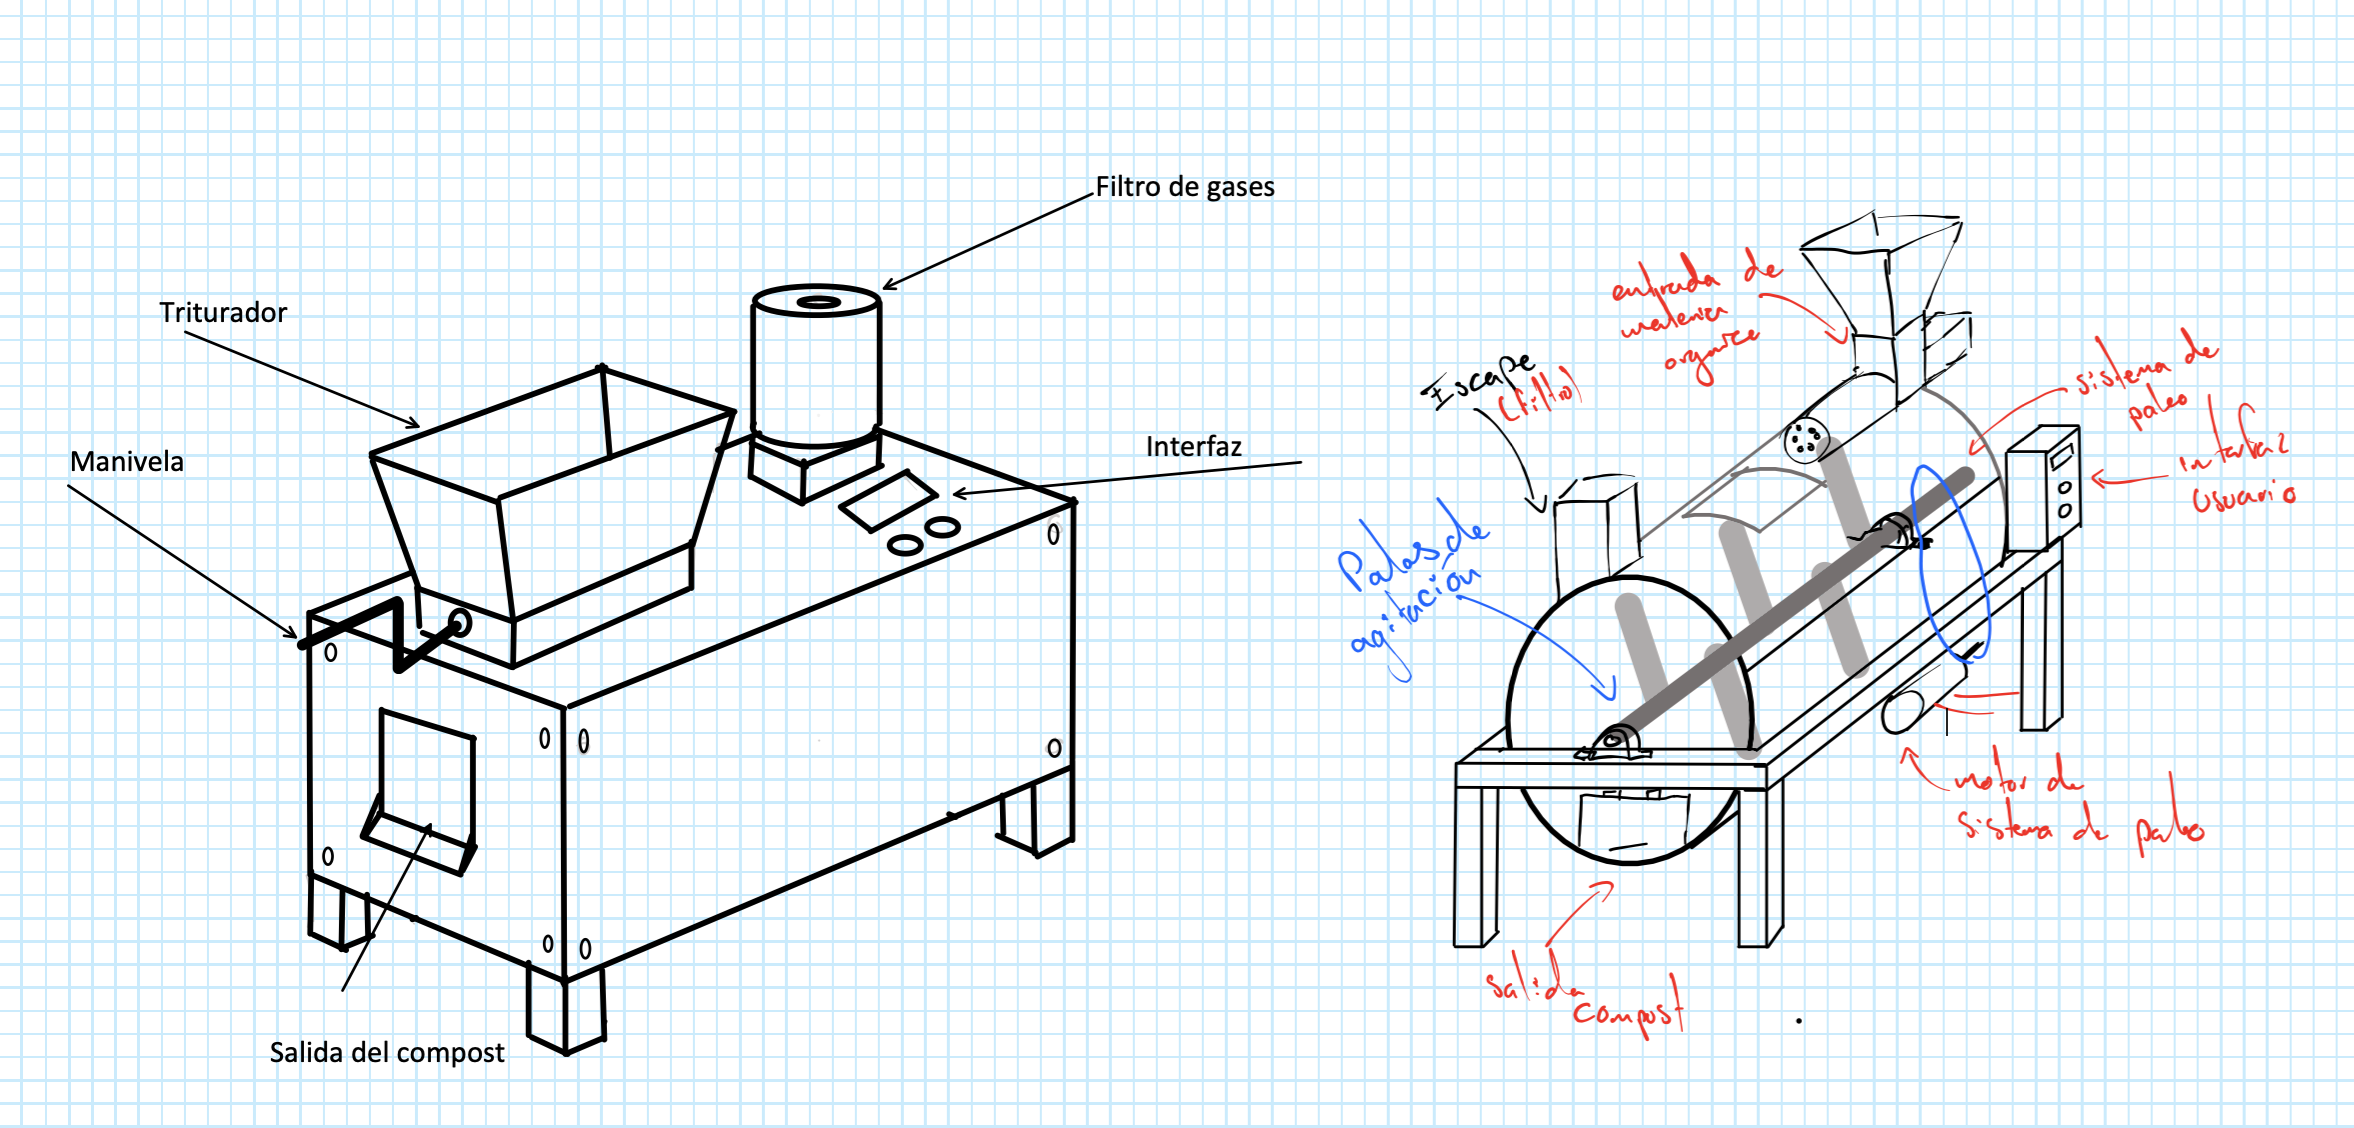
\includegraphics[scale=0.25]{images/Capitulo 3/3.2.5 Diseño Conceptual/ConceptosGenerados.png}
        \caption{Conceptos Generados}
    \label{fg:conceptos}
\end{figure}

\subsection{Validación del sistema}

Con las opciones ya delimitadas por las rutas de diseño en la matriz morfológica, se realiza un análisis numérico utilizando el proceso analítico jerárquico (AHP). Este proceso realiza una evaluación de cada una de las opciones, basado en la ponderación de diversos criterios, que estarán ordenados y ponderados del más importante al más flexible.

Para el caso de este proyecto, los criterios requeridos se han ordenado de la siguiente manera:

\begin{itemize}
    \item Costo.
    \item Facilidad de manufactura
    \item Disponibilidad
    \item Seguridad de uso
    \item Facilidad de uso
    \item Integración
    \item Mantenimiento
    \item Durabilidad
    \item Ergonomía
    \item Portabilidad
    \item Estética
\end{itemize}

Con estos criterios, se realiza una estimación numérica al comparar el peso que tiene un criterio sobre otro. De esta manera, se obtiene un porcentaje que simboliza el peso de cada uno de los criterios al momento de tomar una decisión.

Los cálculos detallados de esta estimación se encuentran en la tabla del apéndice \ref{Ap:Crit}, donde los resultados obtenidos están recopilados en la tabla \ref{tab:Cuanticrit}.

\begin{table}[h]
    \centering
    \caption{Cuantificación de los criterios} 
    \begin{tabular}{|c|c|}
    \hline
        Criterio & Ponderación \% \\ \hline
        Costo &  16.7 \\ \hline
        Facilidad de manufactura & 15.7  \\ \hline
        Disponibilidad & 13.9  \\ \hline
        Seguridad de uso & 13.9 \\ \hline
        Facilidad de uso & 10.2  \\ \hline
        Integración & 8.3  \\ \hline
        Mantenimiento & 7.4 \\ \hline
        Durabilidad & 6.5 \\ \hline
        Ergonomía & 5.6 \\   \hline
        Portabilidad & 0.9  \\  \hline
        Estética & 0.9 \\ \hline
    \end{tabular}
    \label{tab:Cuanticrit}
\end{table}

Con estas ponderaciones, se realiza una nueva hoja de cálculo donde se realiza la ponderación de las diferentes soluciones técnicas mediante las matrices de AHP. Con ayuda de este proceso, se obtiene una calificación, basada en los criterios mencionados, con la cual se puede respaldar la selección de alguna de las opciones.

En este trabajo, los cálculos de las Matrices de AHP están descritos a detalle en el apéndice \ref{Ap:AHPMat}.

\subsection{Selección de diseño conceptual}

Con base en la tabla AHP, después de haber realizado las ponderaciones de acuerdo a los criterios anteriormente mencionados, se obtuvieron los componentes que mejor se adaptaban y que cumplen con las necesidades del proyecto; estos componentes se presentan en la tabla \ref{tab:modeloselec}.

De igual forma, se realizó una discusión para realizar el boceto que englobe mejor las soluciones. El boceto permite ilustrar el diseño conceptual, modelo a partir del cual se realizaron los diseños de los módulos del sistema. El boceto propuesto está en la ilustración \ref{fg:boceto seleccionado}

\begin{table}[h]
    \centering
    \caption{Modelo seleccionado}
    \begin{tabular}{|c|c|}
         \hline
         \rowcolor[rgb]{ .251,  .251,  .251}{\textcolor[rgb]{ 1,  1,  1}{Características}} & {\textcolor[rgb]{ 1,  1,  1}{Selección}} \\
         \hline
         \rowcolor[rgb]{ .886,  .937,  .855}Trituración & Rallador\\
         \hline
         \rowcolor[rgb]{ .867,  .922,  .969}Almacenamiento & Contenedor horizontal\\
         \hline
         \rowcolor[rgb]{ 1,  .949,  .8}Palas de agitación & Palas planas\\
         \hline
         \rowcolor[rgb]{ .929,  .929,  .929}Trasmisión de movimiento & Banda V\\
         \hline
         \rowcolor[rgb]{ .988,  .894,  .839}Medir temperatura & Sensor electrónico\\
         \hline
         \rowcolor[rgb]{ .886,  .937,  .855}Medir humedad & Sensor ambiental\\
         \hline
         \rowcolor[rgb]{ 1,  .949,  .8}Elevar temperatura & Resistencia eléctrica\\
         \hline
         \rowcolor[rgb]{ .929,  .929,  .929}Elevar humedad & Por goteo\\
         \hline
         \rowcolor[rgb]{ .988,  .894,  .839}Oxigenar el sistema & Ventilación directa\\
         \hline
          \rowcolor[rgb]{ .886,  .937,  .855}Unidad de procesamiento & Tarjeta de desarrollo\\
         \hline
         \rowcolor[rgb]{ .867,  .922,  .969}Interfaz hombre-máquina & Botones y pantalla\\
         \hline
    \end{tabular}
    \label{tab:modeloselec}
\end{table}

%La utilidad de este método es la fácil asignación  de valores de todos los diferentes componentes, ya que al tener una gran cantidad de combinaciones posibles era difícil determinar las mejores opciones al tratarse de un sistema que integra a todos ellos en su funcionamiento.


\begin{figure}[h!]
    \centering
        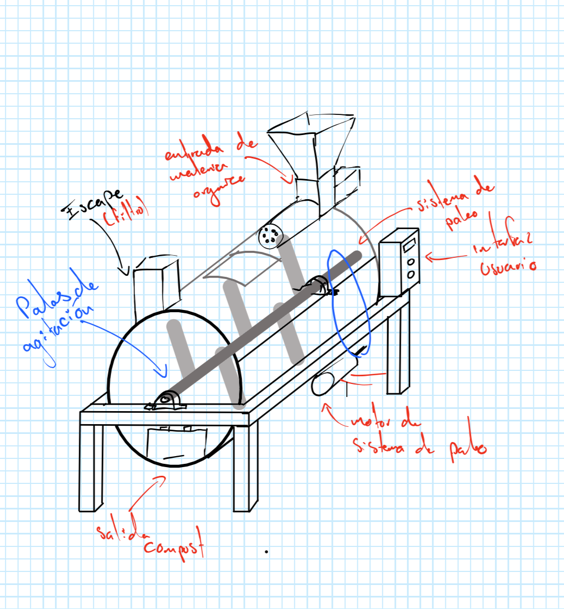
\includegraphics[scale=0.4]{images/Capitulo 3/3.2.5 Diseño Conceptual/Boceto seleccionado.png}
        \caption{Boceto seleccionado}
    \label{fg:boceto seleccionado}
\end{figure}


\newpage


\section{Diseño Específico del Sistema}

En esta parte se realiza el diseño de cada uno de los módulos, incluyendo los componentes de cada una de las soluciones tecnológicas seleccionadas.


\subsection{Sistema de administración de comportamiento $S_1$}

Este es el sistema que realizará la interpretación de los valores obtenidos a partir del \textbf{sistema de procesamiento de datos $S_2$} y a su vez, es el encargado de tomar decisiones basadas en el estado del proceso. También realiza los enlaces con el usuario a través de la interfaz humano - máquina. 

\input{parts/2_Dis_sist/2.2 Diseño especifico/4.1.1 Subsistema1/4.1.1.1 Tarjeta}
\input{parts/2_Dis_sist/2.2 Diseño especifico/4.1.1 Subsistema1/4.1.1.2 Interfaz}
\input{parts/2_Dis_sist/2.2 Diseño especifico/4.1.1 Subsistema1/4.1.1.3 Control}
%Sistema de administración de comportamiento

\newpage

\subsection{Sistema de procesamiento de datos $s_2$}

Para que el sistema pueda tomar decisiones por si mismo  es necesario que pueda leer el estado de los parámetros internos durante el proceso de compostaje. Según la figura \ref{fg:ArchFis} que describe la arquitectura física del sistema, se requiere el diseño de un módulo especial de adquisición de señales, módulos de acondicionamientos de señales y módulos de comunicación interna. 

\input{parts/2_Dis_sist/2.2 Diseño especifico/4.1.2 Subsistema2/4.1.2.1 Adquirir las señales}
\input{parts/2_Dis_sist/2.2 Diseño especifico/4.1.2 Subsistema2/4.1.2.2 Acondicionamiento de señales}
\input{parts/2_Dis_sist/2.2 Diseño especifico/4.1.2 Subsistema2/4.1.2.3 Comunicacion}
%\input{parts/2_Dis_sist/2.2 Diseño especifico/4.1.2 Subsistema2/4.1.2.4 Validacion}
%Sistema de procesamiento de datos

\subsection{Sistema de energía $S_3$}

\input{parts/2_Dis_sist/2.2 Diseño especifico/4.1.3 Subsistema 3/4.1.3.1 Diseno}
\input{parts/2_Dis_sist/2.2 Diseño especifico/4.1.3 Subsistema 3/4.1.3.2 Validación}
%Sistema de energía

\subsection{Trituración $S_4$}

El sistema de trituración es un sistema manual del compostador, de ahí el nombre sistema semi-automatico.

La potencia con la que trabaja este sistema de trituración esta directamente relacionado con la fuerza que un ser humano puede generar al girar un brazo de palanca, por lo que el sistema esta limitado en gran medida en comparación de lo que sería un sistema totalmente automático accionado por un motor (\ref{fg:brazo}).


\begin{figure}[h!]
            \centering
            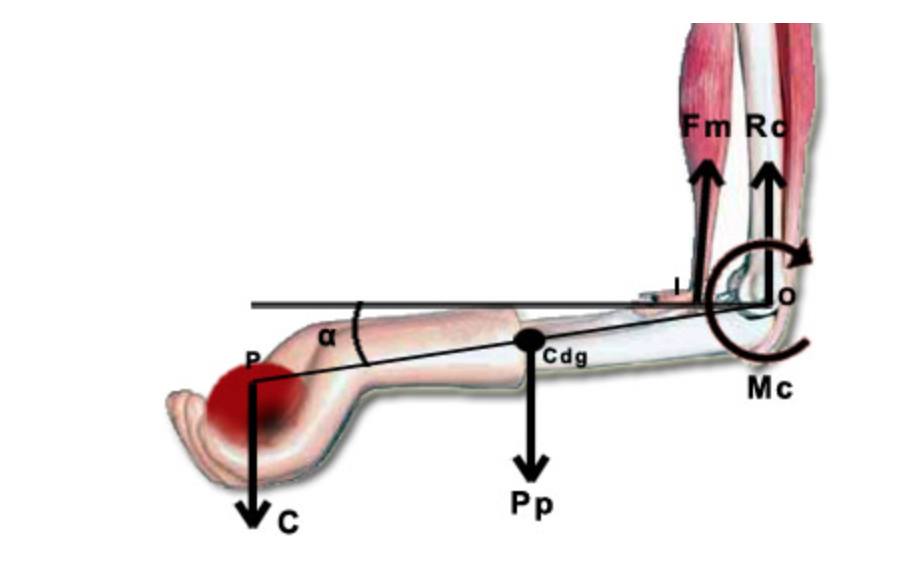
\includegraphics[scale=0.5]{images/Capitulo 4/S4/Brazo de Palanca Humana.png}
            \caption{Brazo de Palanca Humana}
            \cite{Biomec}
            \label{fg:brazo}
\end{figure}

\input{parts/2_Dis_sist/2.2 Diseño especifico/4.1.4 Subsistema 4/4.1.4.1 Diseno}
\input{parts/2_Dis_sist/2.2 Diseño especifico/4.1.4 Subsistema 4/4.1.4.2 Validación}
%Trituración 

\subsection{Sistema de procesamiento de materia $S_5$}

\input{parts/2_Dis_sist/2.2 Diseño especifico/4.1.5 Subsistema 5/4.1.5.1 Diseno del contenedor}

\input{parts/2_Dis_sist/2.2 Diseño especifico/4.1.5 Subsistema 5/4.1.5.2 Temperatura}

\input{parts/2_Dis_sist/2.2 Diseño especifico/4.1.5 Subsistema 5/4.1.5.3 Riego}

\input{parts/2_Dis_sist/2.2 Diseño especifico/4.1.5 Subsistema 5/4.1.5.4 Ventilacion}

\input{parts/2_Dis_sist/2.2 Diseño especifico/4.1.5 Subsistema 5/4.1.5.5 Circuitos de actuadores}

\input{parts/2_Dis_sist/2.2 Diseño especifico/4.1.5 Subsistema 5/4.1.5.6 Aireación/4.1.5.6.0 AireacionS}



%Sistema de procesamiento de materia

\subsection{Sistema estructural $S_6$}

El diseño estructural es una parte clave en el desarrollo del proyecto, sin una estructura con la suficiente resistencia mecánica, la integridad de todo se ve comprometida.

Además una buena estructura permite colocar todas los componentes necesarios para su correcto funcionamiento, sin necesidad de hacer complicados sistemas de sujeción para los distintos componentes

\input{parts/2_Dis_sist/2.2 Diseño especifico/4.1.6 Subsistema 6/4.1.6.1 Diseno}

\input{parts/2_Dis_sist/2.2 Diseño especifico/4.1.6 Subsistema 6/4.1.6.2 Validación}

\input{parts/2_Dis_sist/2.2 Diseño especifico/4.1.6 Subsistema 6/4.1.6.3 Integracion}
%sistema estructural

%%%modificar archivo capitulos/diseconceptual.tex
%%%%%%%%%%%%%%%%%%%%%%%%%%%%%%%%%%%%%%%%%%%%%%%%%%%%%%%%%%%%%%%%%%%
%%%%%%%%%%%%%%%%%%%%%%%%%%%%%%%%%%%%%%%%%%%%%%%%%%%%%%%%%%%%%%%%%%%
%\include{capitulos/disedetallado}
%%%modificar archivo capitulos/disedetallado.tex
%%%%%%%%%%%%%%%%%%%%%%%%%%%%%%%%%%%%%%%%%%%%%%%%%%%%%%%%%%%%%%%%%%%

\chapter{Implementación del sistema}

\subsection{Sistema de administración de comportamiento $S_1$}

\textbf{Implementación de la tarjeta de desarrollo e humano-máquina}

Para el funcionamiento del software del sistema mecatrónico, se implementó una tarjeta ESP32, la cual se montó en un protoboard para realizar las conexiones necesarias para el funcionamiento del circuito electrónico principal. 

Para la implementación, se realizo un código (Apéndice \ref{Ap:Codigo_completo}) en lenguaje C a través de la interfaz de Arduino 2.0. El código está formado por 4 hilos, que son diferentes rutinas que se ejecutan de manera simultanea dentro de los procesadores del microcontrolador.

Las diferentes subrutinas se comunican por medio de banderas internas, declaradas al interior del código para coordinar a los distintos actuadores. 

El hilo principal, se encarga de recibir la señal  de inicio al proceso de compostaje, arrancando la interfaz, también se encarga de iniciar los registros necesarios para verificar el avance del tiempo. 

Un segundo hilo es el encargado de registrar el tiempo general del proceso, sumando una unidad a un registro llamado "Segundos" cada vez que se realiza una pausa con un periodo de 1 segundo. En este mismo hilo, se realiza una secuencia de instrucciones para agrupar los minutos y las horas para al final, cuando se cumpla el ciclo total de 72 horas, mandará una bandera que indique el fin del proceso y detenga las tareas de los actuadores.

El tercer hilo se encarga de coordinar los proceso de aireación, los cuales activarán el eje de aireación junto al sistema de ventilación por 10 minutos cada 3 horas, para mezclar y oxigenar los residuos.

El último hilo, se encarga de leer los valores recopilados de los sensores de DHT11 (Humedad) y el DS18B20 (Temperatura) y realizar las etapas de control de encendido de los procesos de regulación de temperatura y regulación de humedad.

Para poder interactuar con el dispositivo, dentro del hilo principal, se ha implementado una interfaz (figura \ref{fg:cto_interfaz_fisico}), aquí se han colocado los botones (Figura \ref{fg:botones_imp}), para permitir que el usuario demande cierto tipo de información que estará disponible por medio de un menú.

\begin{figure}[h]
            \centering
            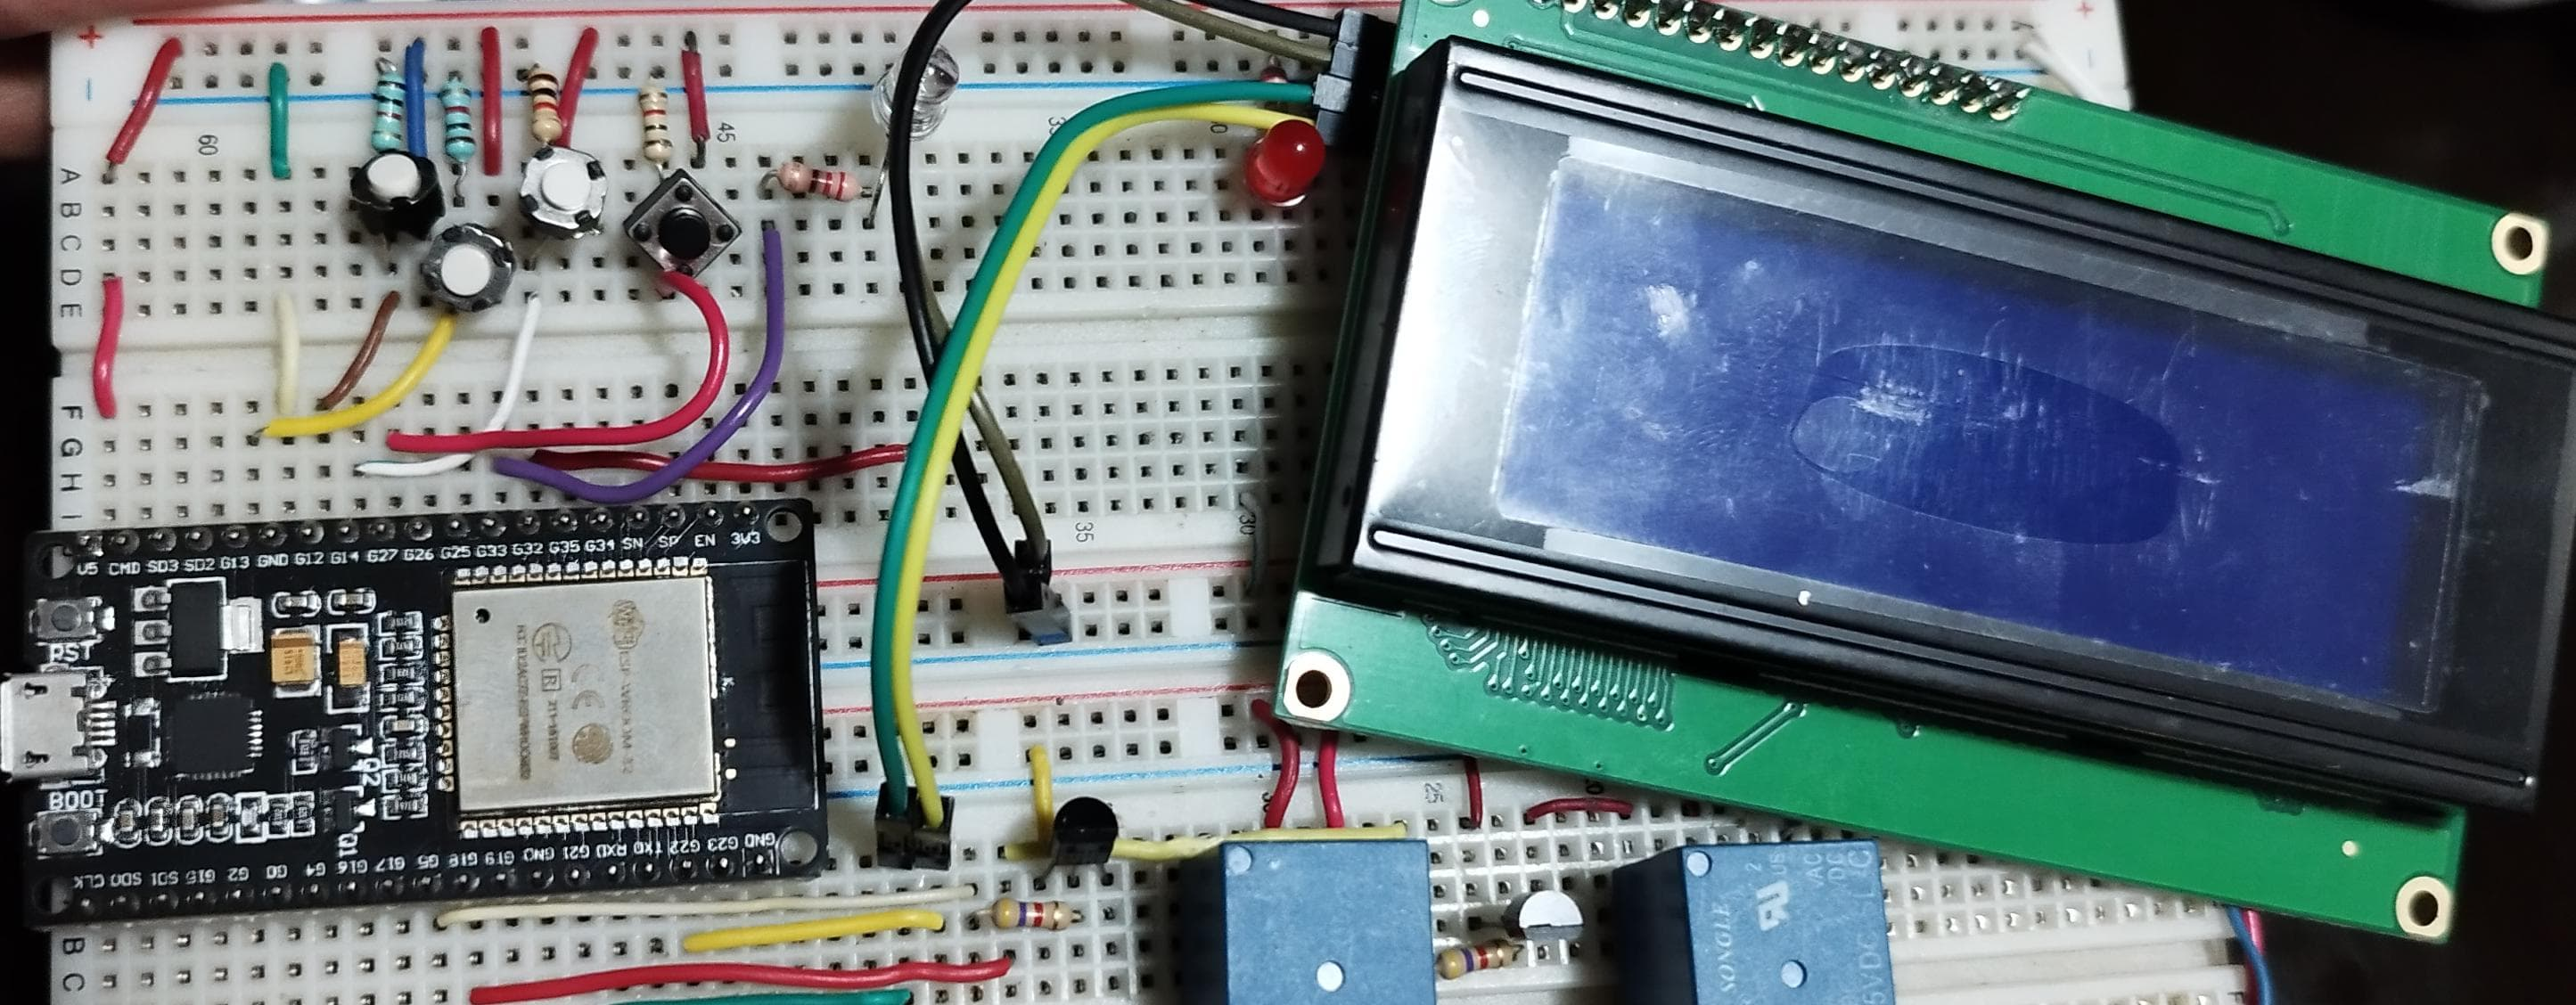
\includegraphics[scale=0.1]{images/Capitulo_Imple/S1/interfaz/cto_interfaz_imp.jpeg}
            \caption{Circuito de prueba de la interfaz}
            \label{fg:cto_interfaz_fisico}
        \end{figure}

\begin{figure}[h]
            \centering
            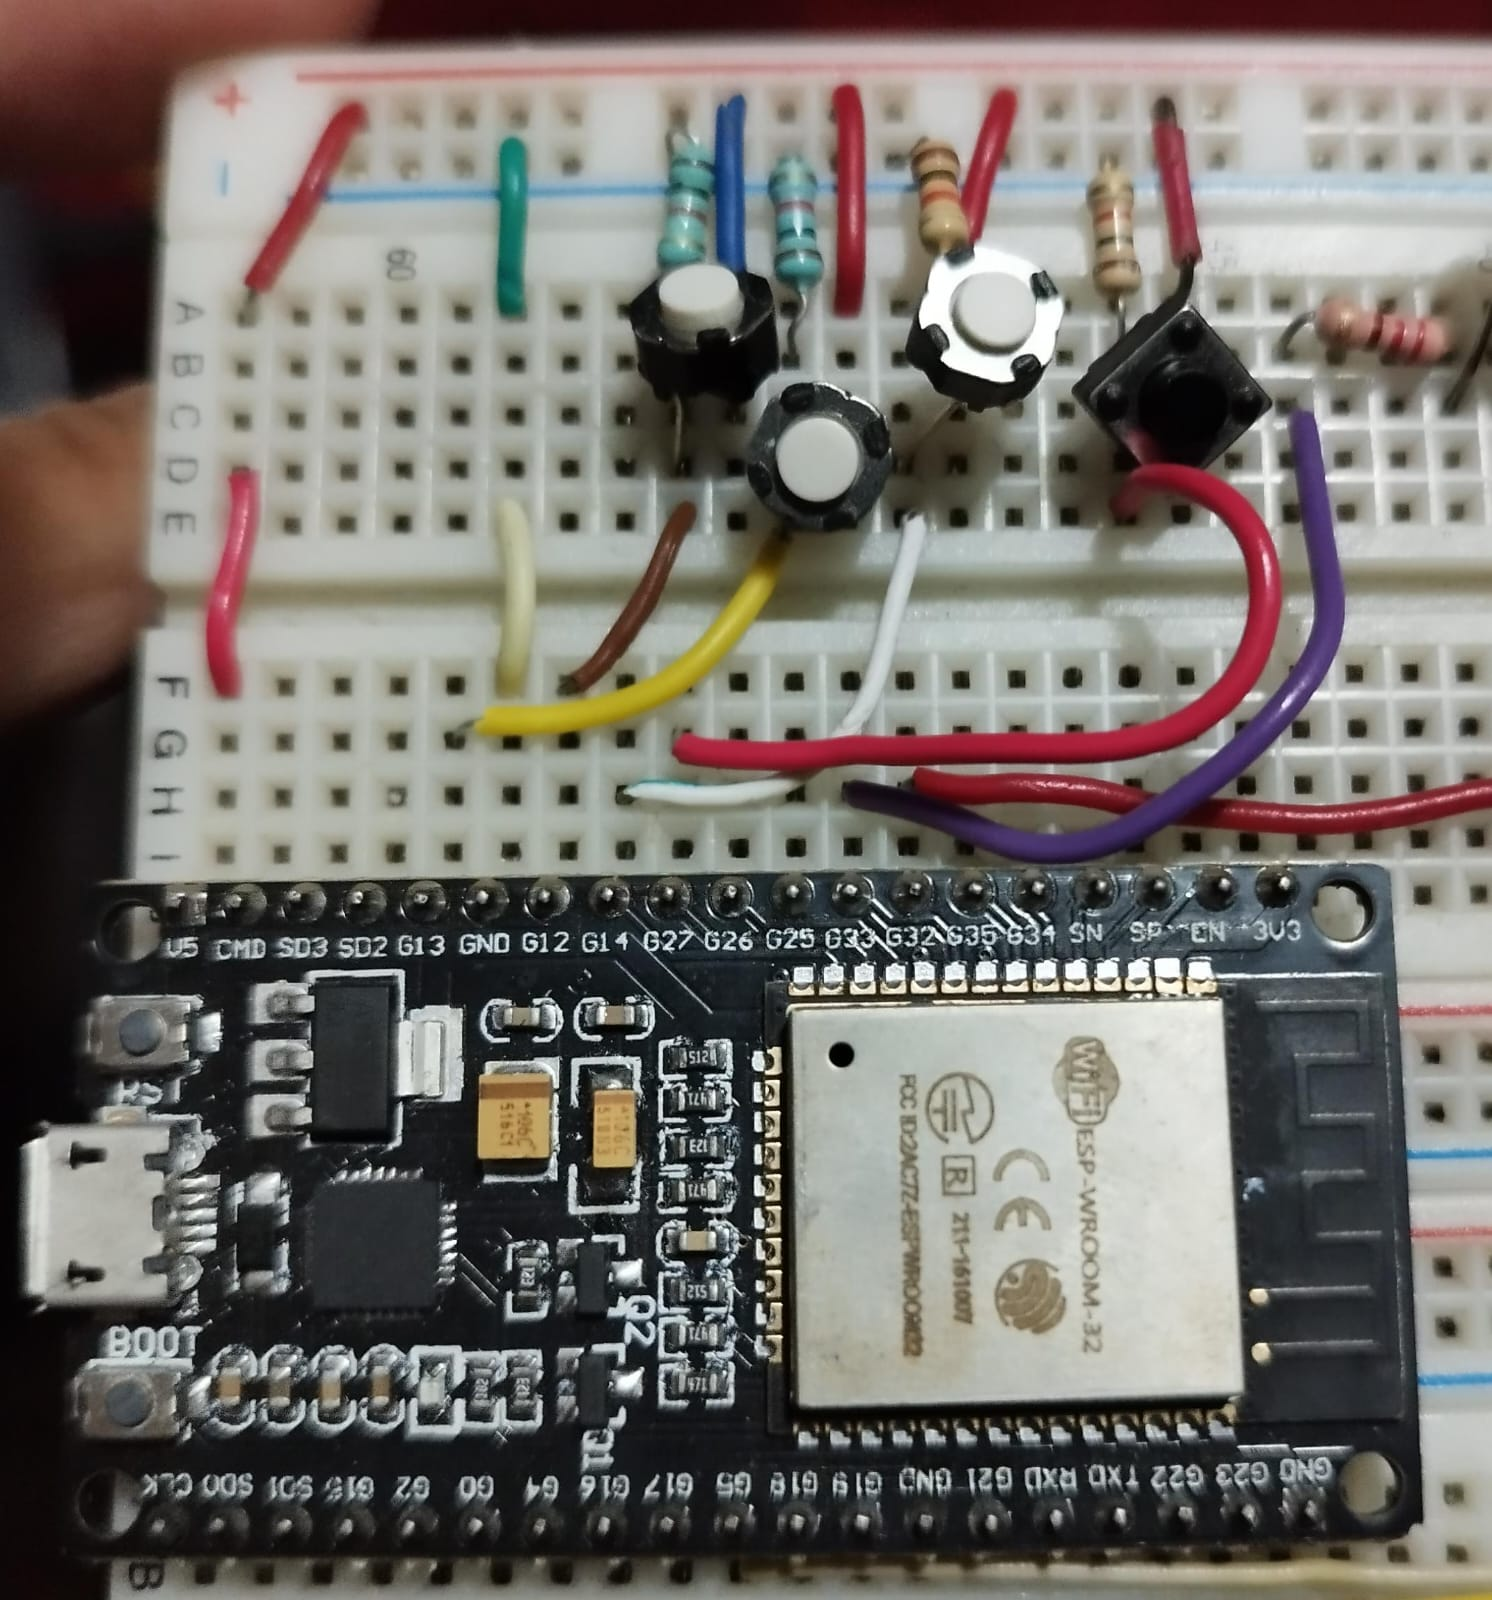
\includegraphics[scale=0.1]{images/Capitulo_Imple/S1/interfaz/botones_int.jpeg}
            \caption{Implementación de los botones}
            \label{fg:botones_imp}
        \end{figure}

\clearpage
Cada uno de los botones, representará cada una de las opciones que se presentarán en el menú (figura \ref{fg:menu_interfaz}) a través de la cual se podrá consultar información relevante acerca del ciclo de procesamiento del compost. Por ejemplo, los mensajes mostrados en las figuras \ref{fg:tiempo_proceso} y \ref{fg:proceso_en_ejecucion}.

\begin{figure}[h]
            \centering
            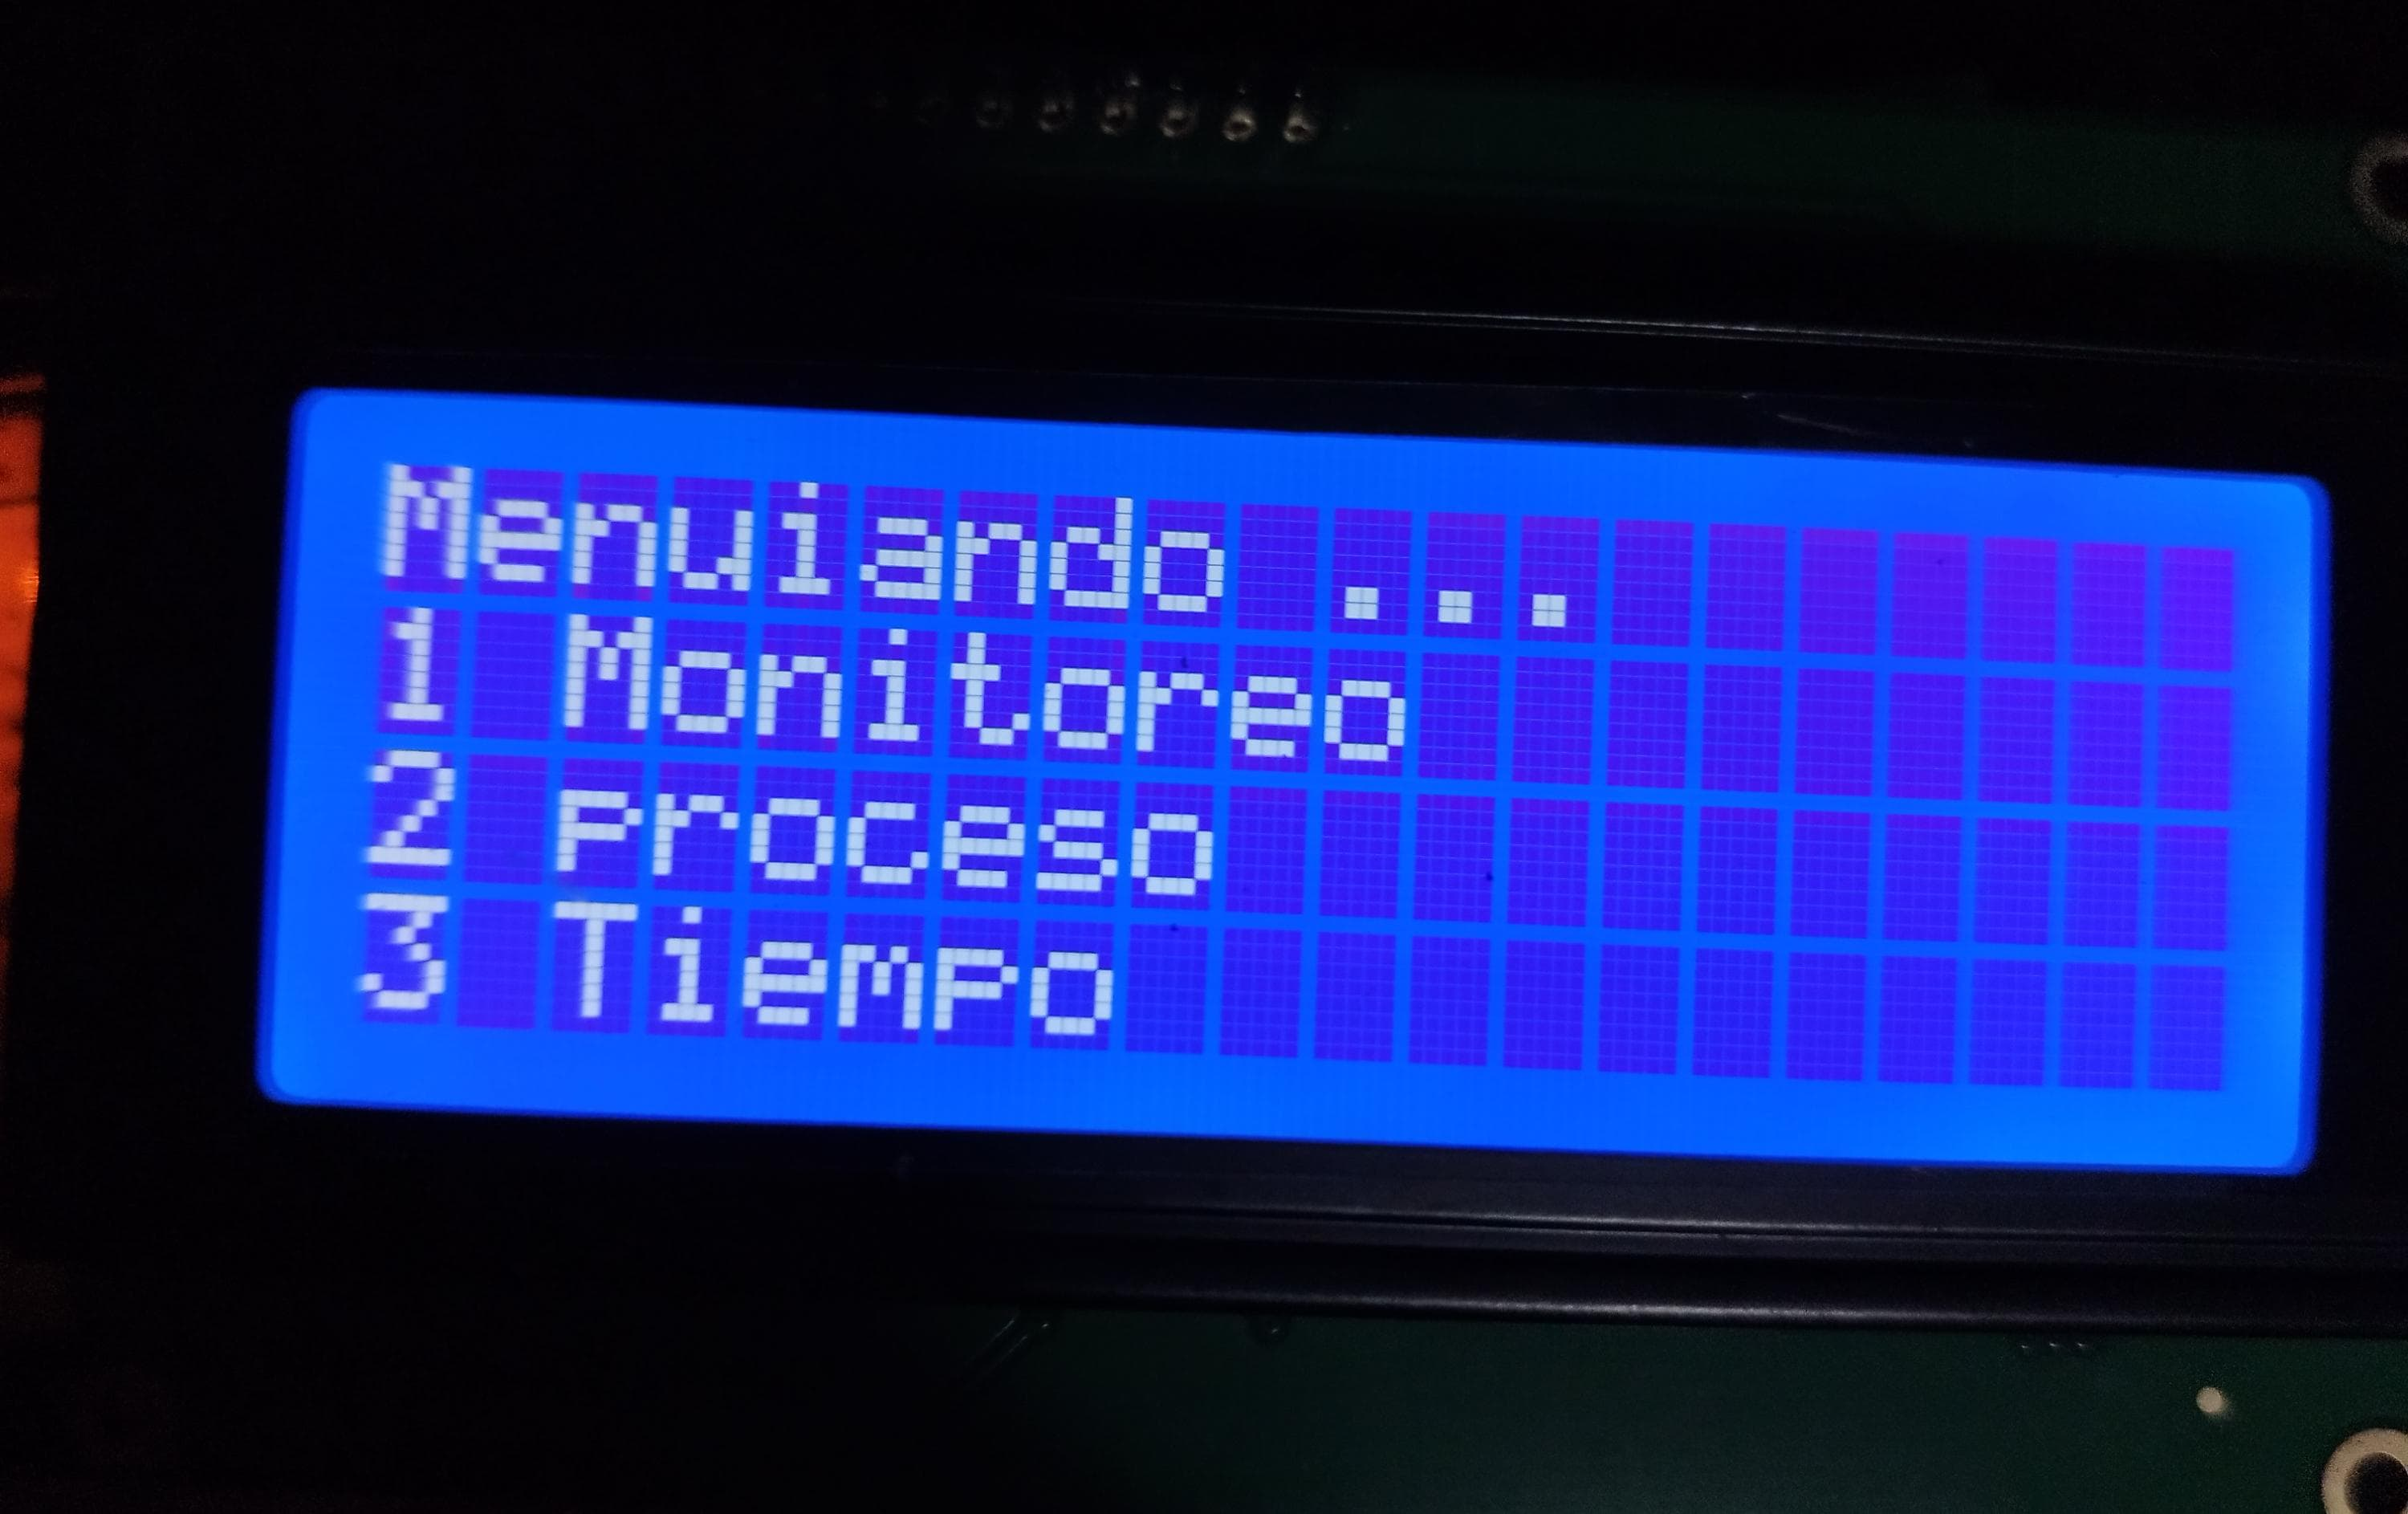
\includegraphics[scale=0.0555]{images/Capitulo_Imple/S1/interfaz/menu.jpeg}
            \caption{Menú desplegado por la interfaz}
            \label{fg:menu_interfaz}
        \end{figure}

\begin{figure}[h]
            \centering
            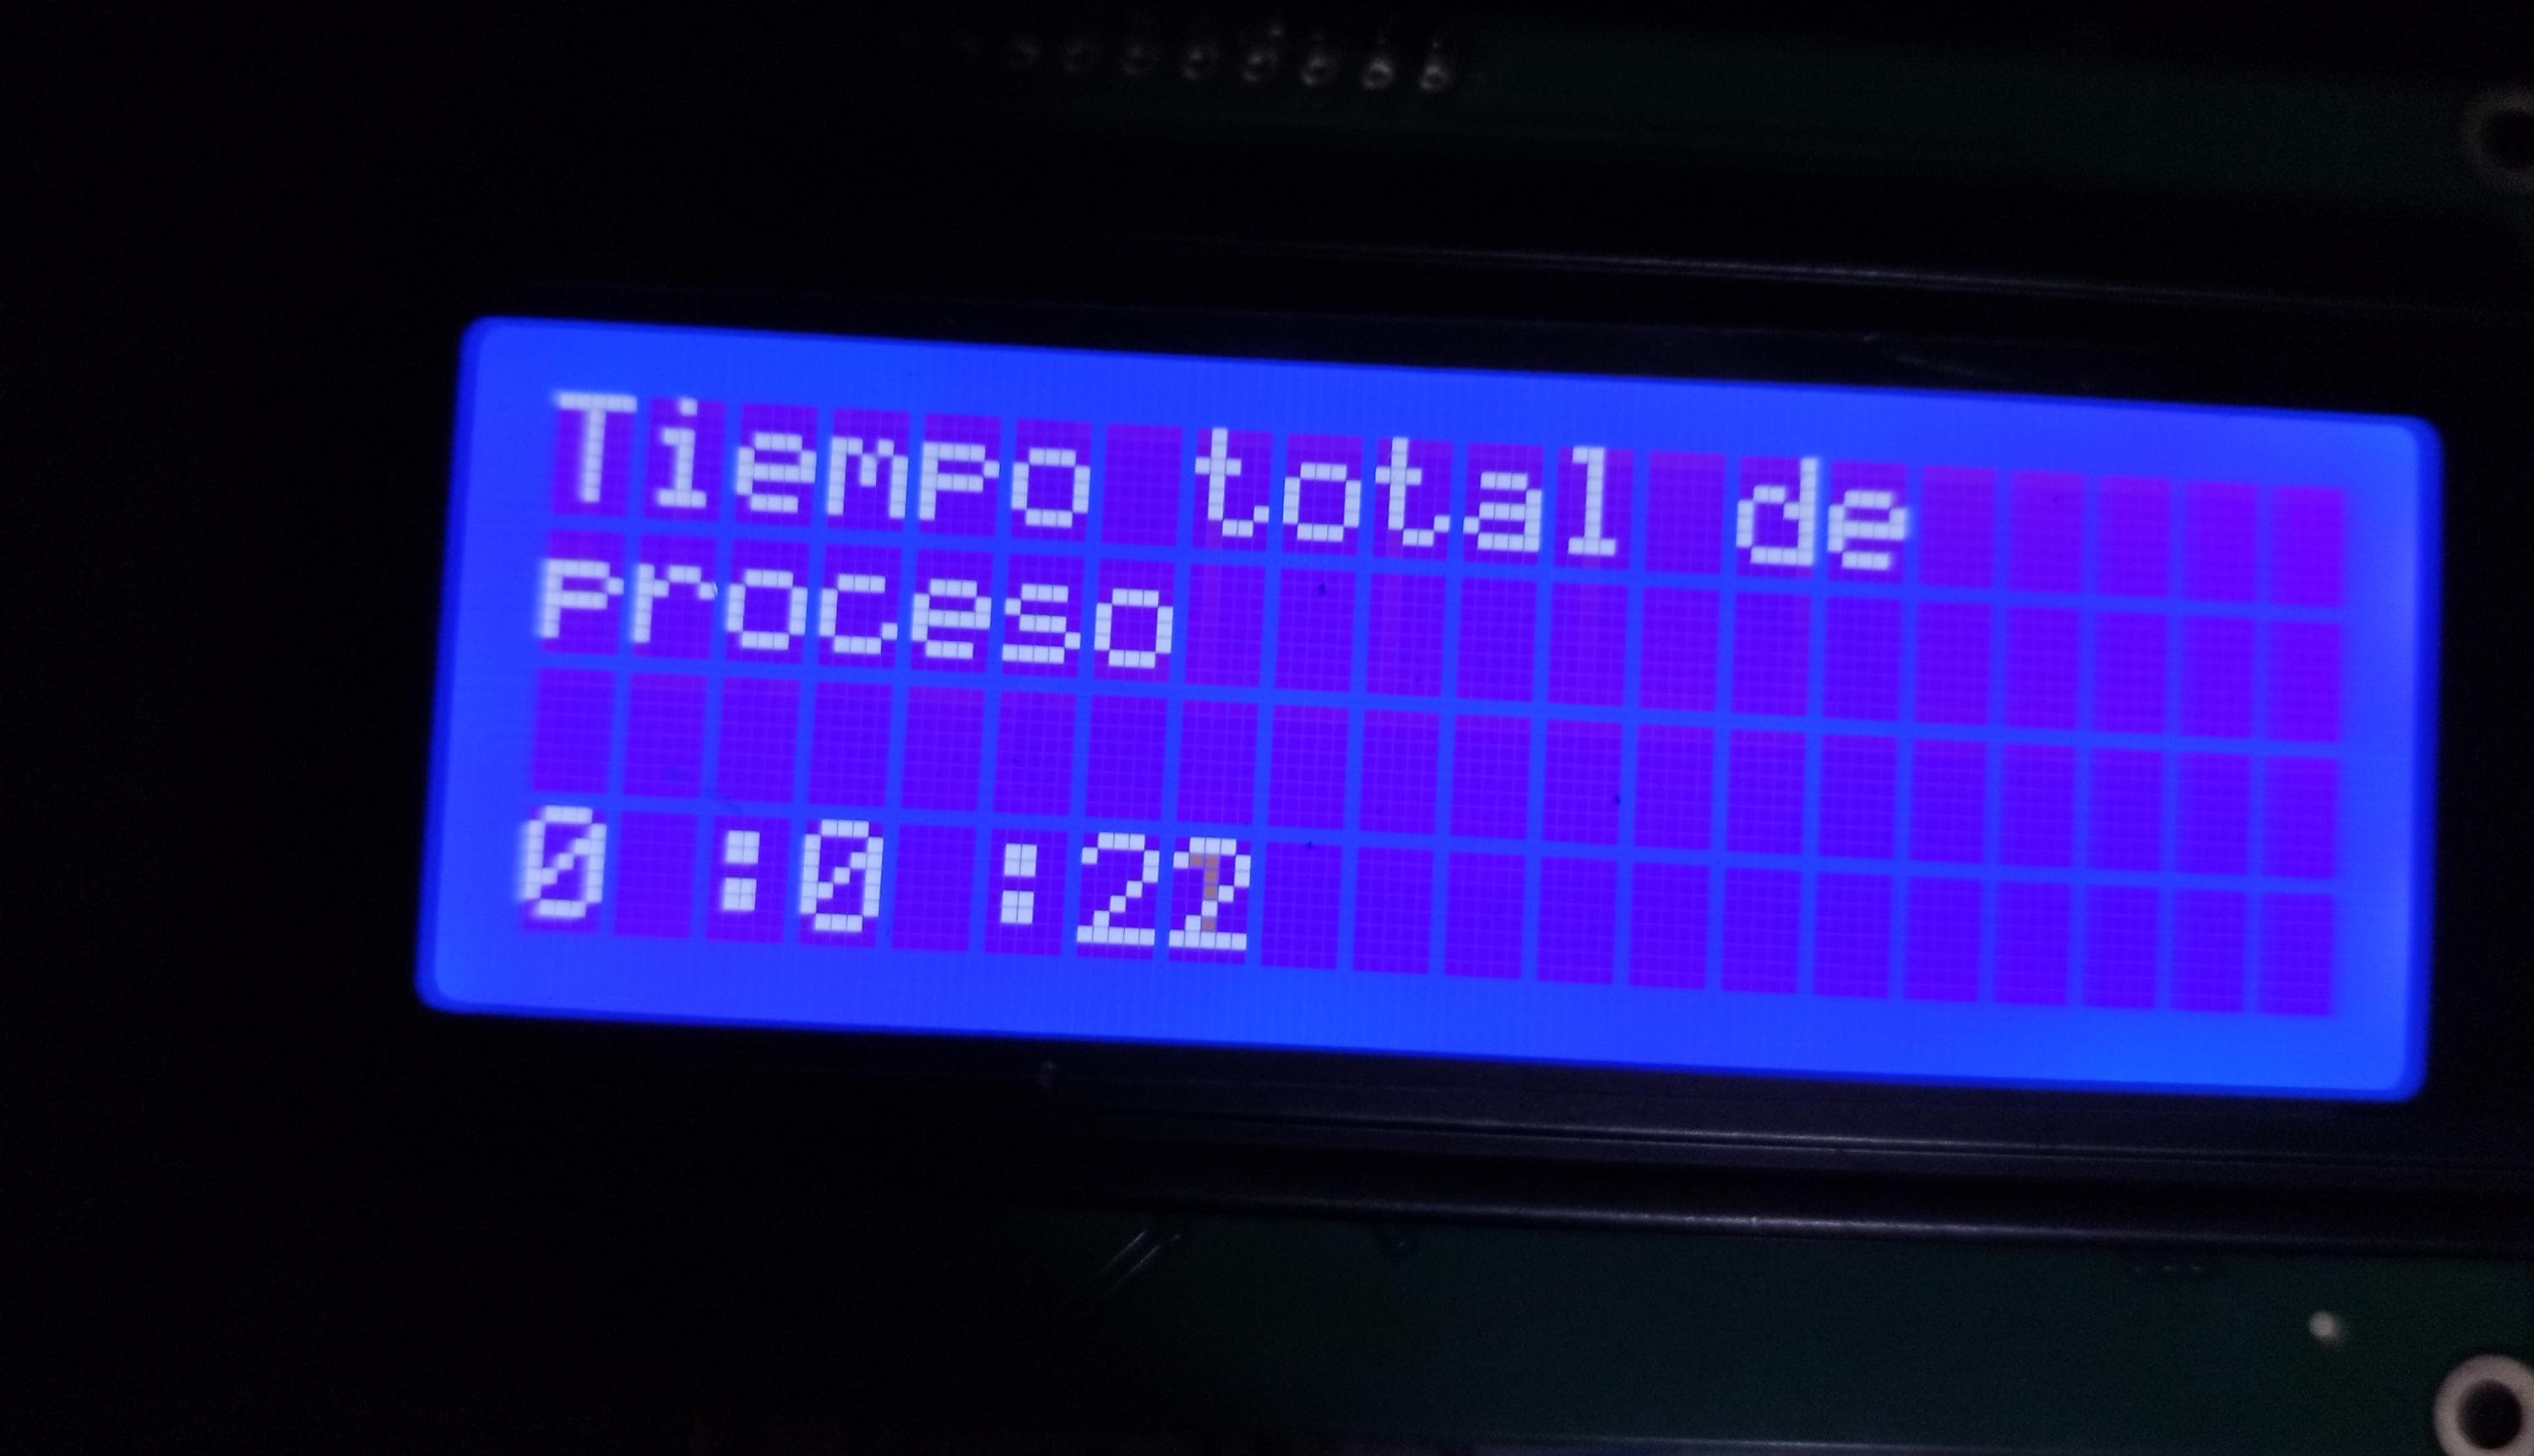
\includegraphics[scale=0.0555]{images/Capitulo_Imple/S1/interfaz/tiempo.jpeg}
            \caption{Representación del tiempo del proceso}
            \label{fg:tiempo_proceso}
        \end{figure}

\begin{figure}[h]
            \centering
            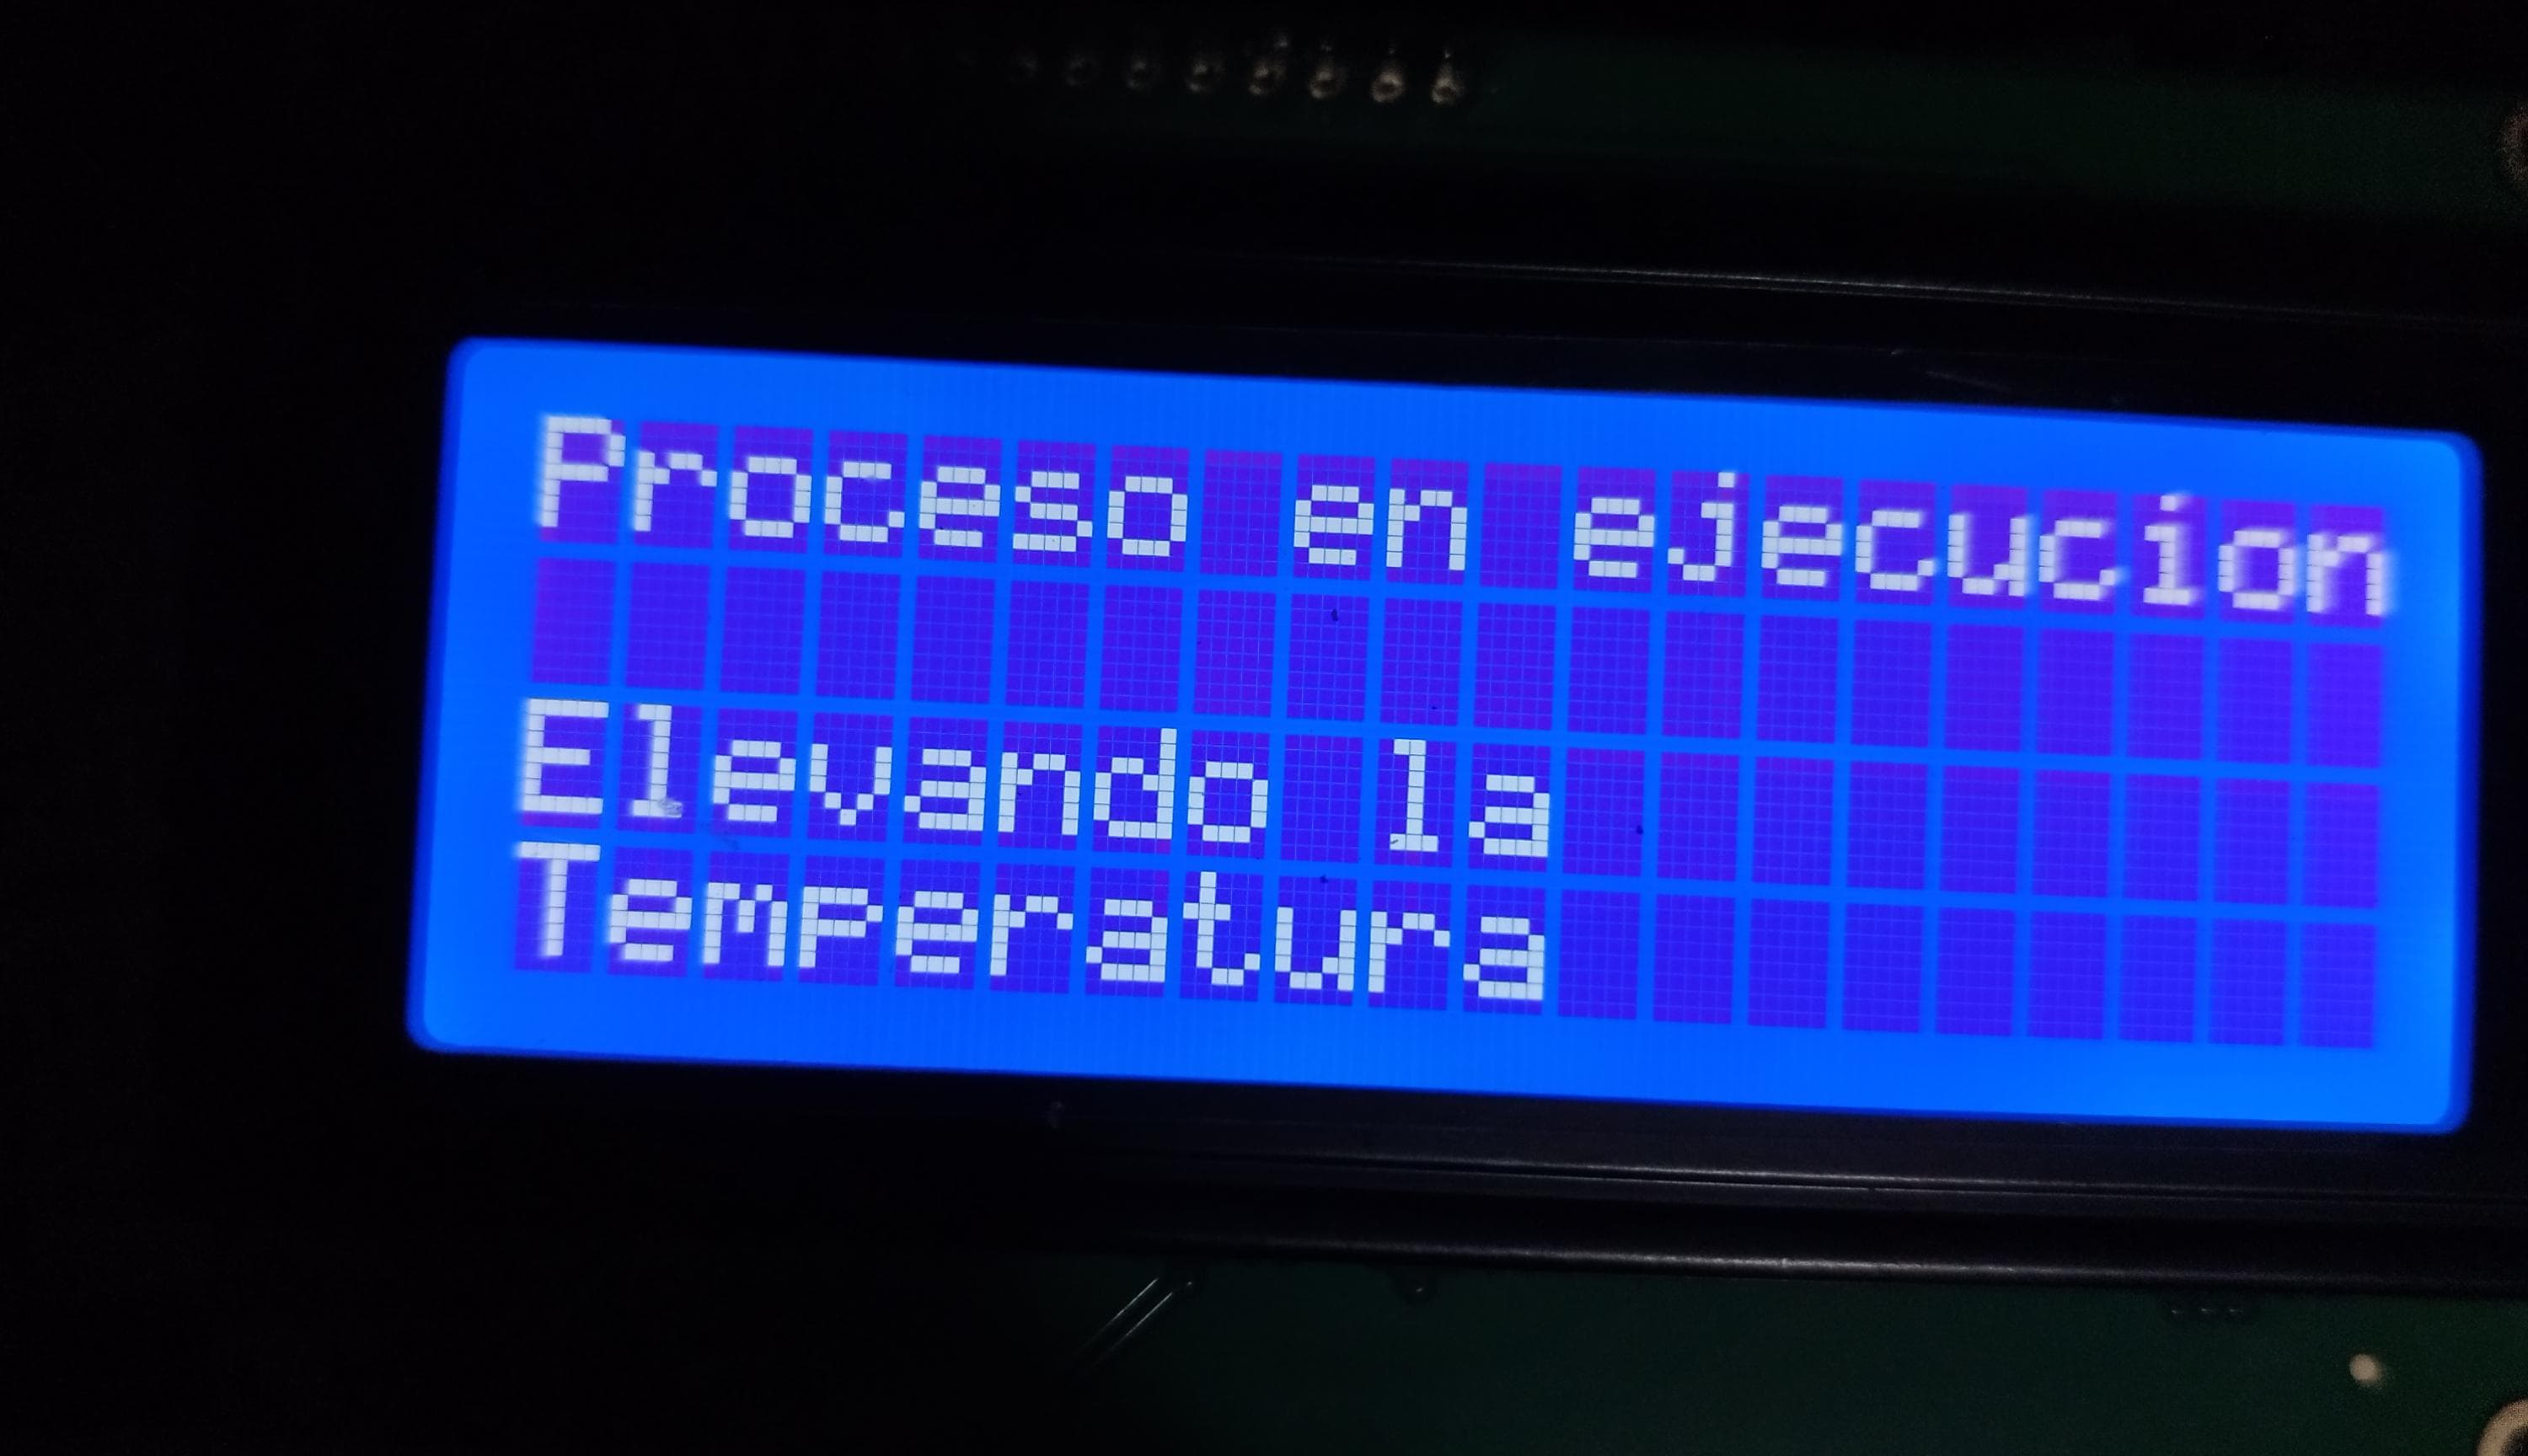
\includegraphics[scale=0.0555]{images/Capitulo_Imple/S1/interfaz/proceso.jpeg}
            
            \caption{Identificación del proceso en ejecución}
            \label{fg:proceso_en_ejecucion}
        \end{figure}
\textbf{Implementación monitoreo a distancia}
Durante la elaboración de este proyecto, se observó que la ESP32 es un microcontrolador bastante robusto y que posee distintas características, dentro de ellas se encuentra la conexión Wi-Fi. Buscando mejorar la experiencia del usuario se consideró que era posible monitorear el funcionamiento del dispositivo a distancia. Por tal motivo se propuso enviar las mediciones realizadas por los sensores a una pagina web para que el usuario pueda acceder de manera remota mediante un link y pueda observar el estado del dispositivo.
La página web para escritorio posee la siguiente distribución:
\begin{figure}[h]
            \centering
            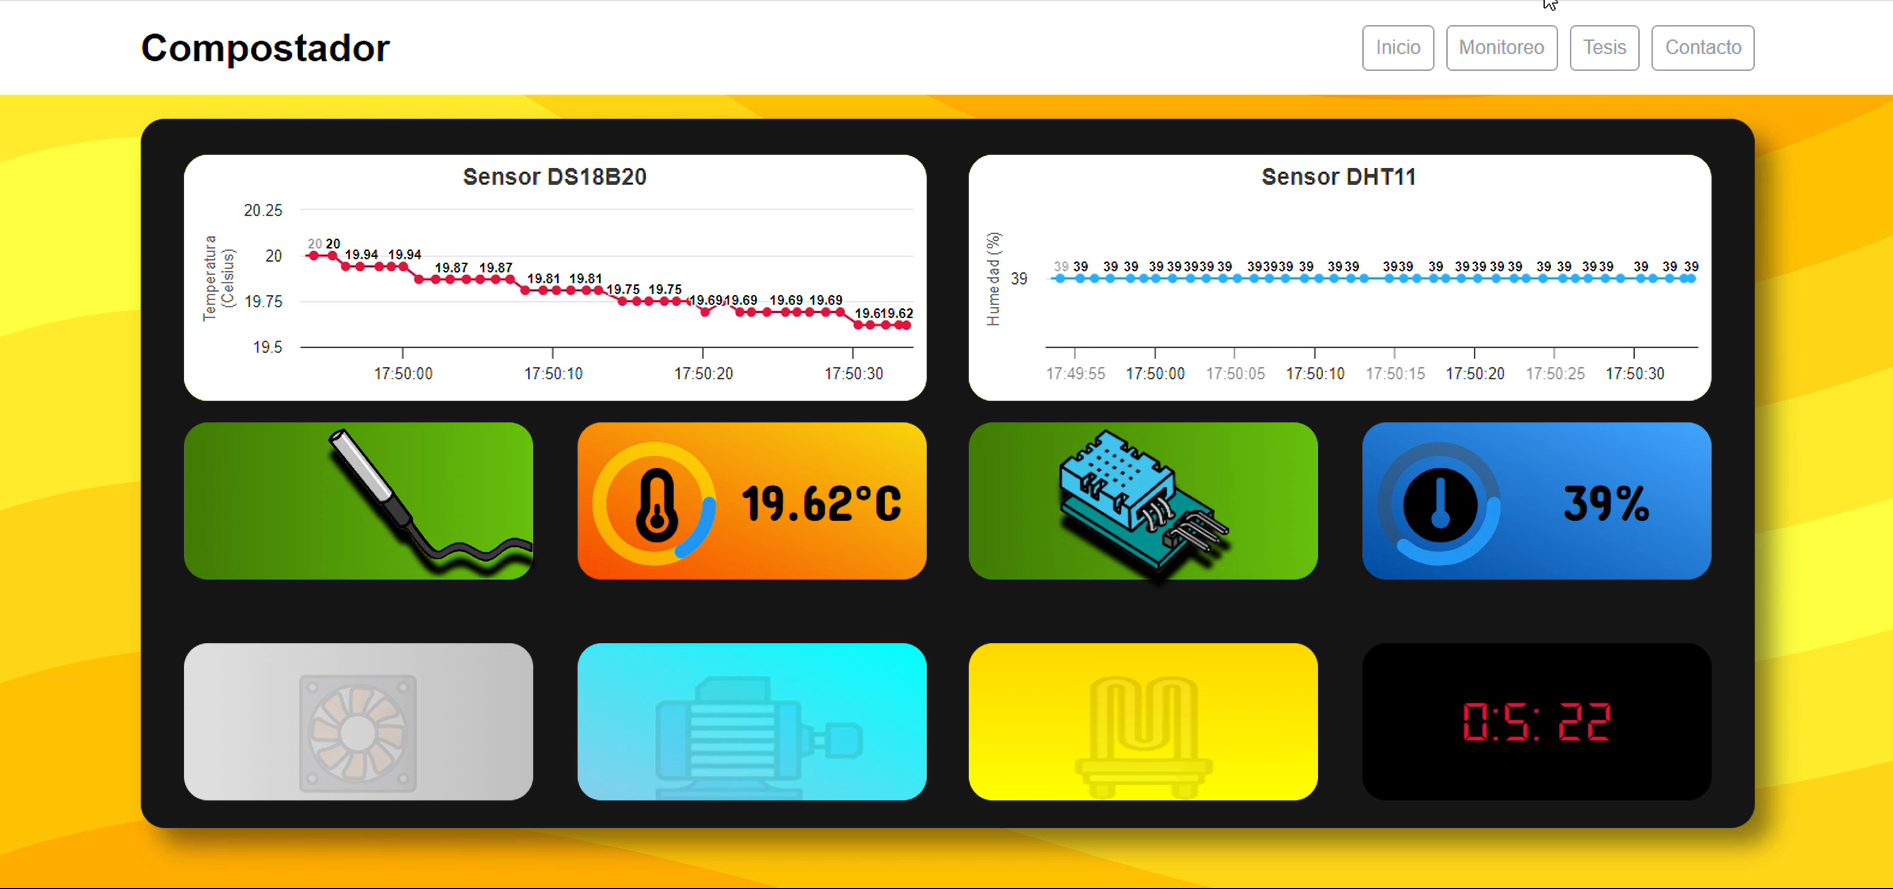
\includegraphics[scale=0.1]{images/Web/pagina_compostador.png}
            
            \caption{Página web compostador}
            \label{fg:pagina_web}
        \end{figure}
Partiendo de la parte superior, se presenta el estado de los sensores tanto de temperatura(DS18B20) como de humedad (DHT11). De primera mano se presenta una grafica con las últimas 40 mediciones enviadas cada segundo, esta gráfica se va actualizando. Sin embargo pensando en la posibilidad de que no todos los usuarios saben interpretar una gráfica, se propuso mostrar el valor de la temperatura  y la humedad en un formato sencillo como si se tratara de la lectura de un termómetro.

\begin{figure}[h]
            \centering
            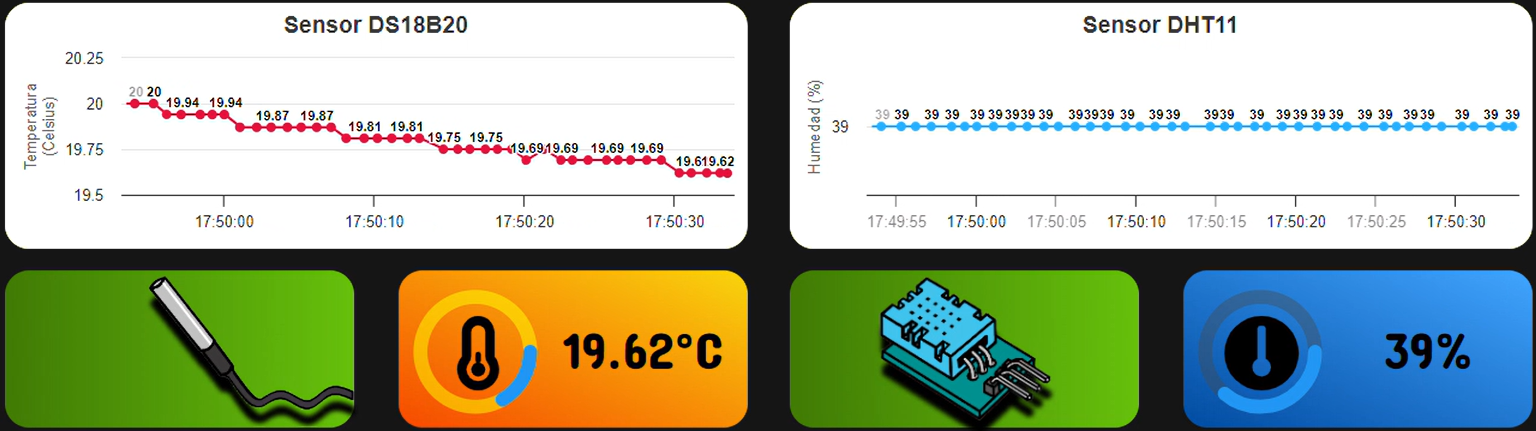
\includegraphics[scale=0.1]{images/Web/temp_hum_web.png}
            
            \caption{Estado sensor DS18B20 y DHT11}
            \label{fg:pagina_web}
        \end{figure}
                 Este indicador busca ser amigable con el usuario, se colocó un ícono de termómetro para que el usuario pueda asociarlo a la temperatura del sistema, el cual reacciona bajo ciertas condiciones previamente programadas ya que conforme este aumenta o disminuye la temperatura este reacciona a los cambios, por otro lado también se colocó un círculo que se va iluminando conforme la temperatura avanza en porcentaje. Conforme a los rangos de temperatura, este círculo cambia de color es decir, en un rango de temperatura mayor a los 0°C pero menor a los 20°C el circulo se iluminará de color azul cielo indicando al usuario una temperatura baja, cuando la temperatura es mayor de 20°C pero menor a 50°C el círculo se iluminará de color naranja y en temperaturas mayores a 50°C será rojo indicando alta temperatura.
            
                \begin{figure}[h]
               \centering
            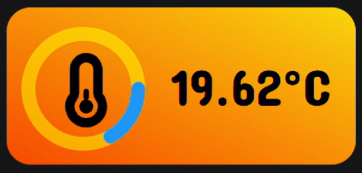
\includegraphics[scale=0.1]{images/Web/indicador.png}
            
            \caption{Indicador de temperatura baja}
            \label{fg:pagina_web}
        \end{figure}
\begin{figure}[h]
            \centering
            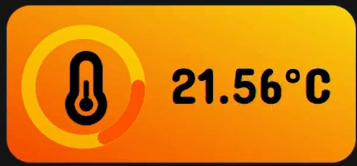
\includegraphics[scale=0.1]{images/Web/indicador_temp.png}
            
            \caption{Indicador temperatura media}
            \label{fg:pagina_web}
        \end{figure}
        Como en todo sensor existe la posibilidad de una falla en la lectura o de un daño en el componente, por lo que se propuso alertar al usuario cuando esto suceda.
        En el caso del sensor DS18B20 cuando este falle arrojará una medición de 0°C, además la casilla donde se encuentra representado el sensor, se iluminará de rojo, y en el indicador de temperatura el círculo se irá a cero así como el termómetro simulará no tener medición. 
\begin{figure}[h]
            \centering
            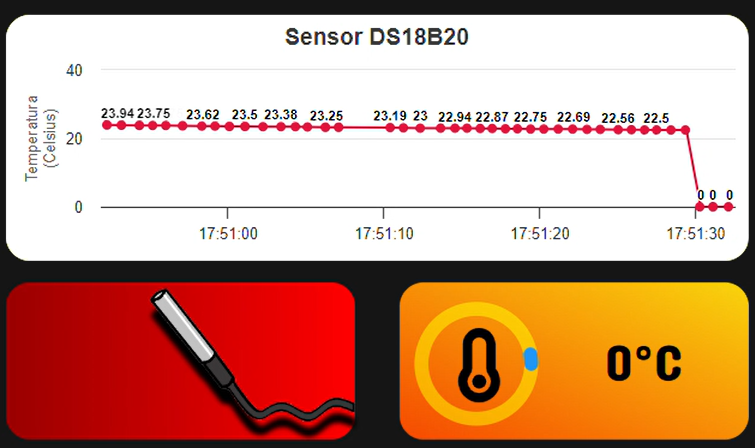
\includegraphics[scale=0.1]{images/Web/error_ds18.png}
            
            \caption{Error sensor DS18B20}
            \label{fg:pagina_web}
        \end{figure}
        En el caso del sensor de humedad, pasa algo similar, siendo que aquí se visualiza la lectura NaN\% (Not a Number) , de igual manera la casilla se iluminará de rojo y el indicador que simula un higrómetro analógico se irá a cero y el circulo también.
        \begin{figure}[h]
            \centering
            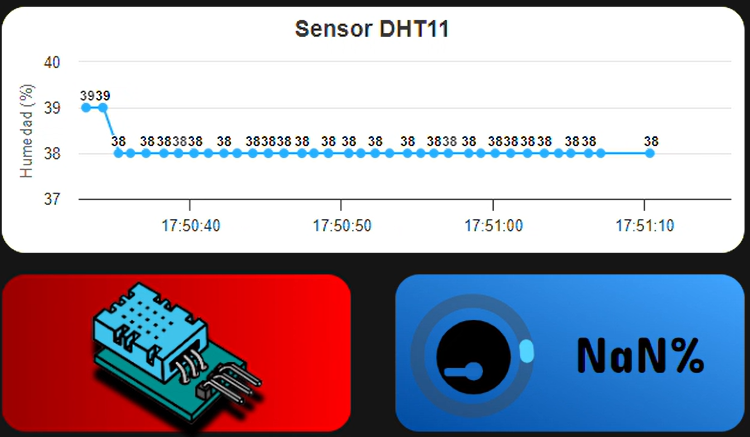
\includegraphics[scale=0.1]{images/Web/dht11_web.png}
            
            \caption{Error sensor DHT11}
            \label{fg:pagina_web}
        \end{figure}
Durante el proceso de compostaje se requiere activar algunos componentes como es el caso de un ventilador, un motor y el cinturón para calentar el tambo. Sin embargo saber que están activados podría ser útil para el usuario, por lo que cada que se enciende alguno de estos dispositivos, se ejecuta una animación que indica el estado de funcionamiento, cuando se apagan, la animación se detiene simulando un estado de pausa.
\begin{figure}[h]
            \centering
            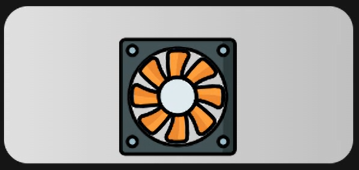
\includegraphics[scale=0.1]{images/Web/ventilador_web.png}
            
            \caption{Activación ventilador}
            \label{fg:pagina_web}
        \end{figure}
\begin{figure}[h]
            \centering
            
\includegraphics[scale=0.1]{images/Web/motor_web.png}
            
            \caption{Activación motor}
            \label{fg:pagina_web}
        \end{figure}
        \begin{figure}[h]
            \centering
            
\includegraphics[scale=0.1]{images/Web/resistencia_web.png}
            
            \caption{Activación resistencia}
            \label{fg:pagina_web}
        \end{figure}
        Por último para saber en qué punto del proceso se encuentra, se colocó un temporizador regresivo que mediante el almacenamiento local de la página registra la hora y aunque la pagina web se actualiza, el temporizador no se reinicia.
\begin{figure}[h]
            \centering
            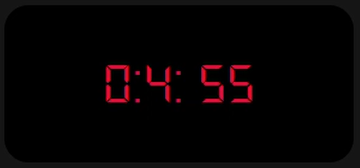
\includegraphics[scale=0.1]{images/Web/temporizador_web.png}
            
            \caption{Temporizador regresivo}
            \label{fg:pagina_web}
        \end{figure}
\begin{figure}[h]
            \centering
            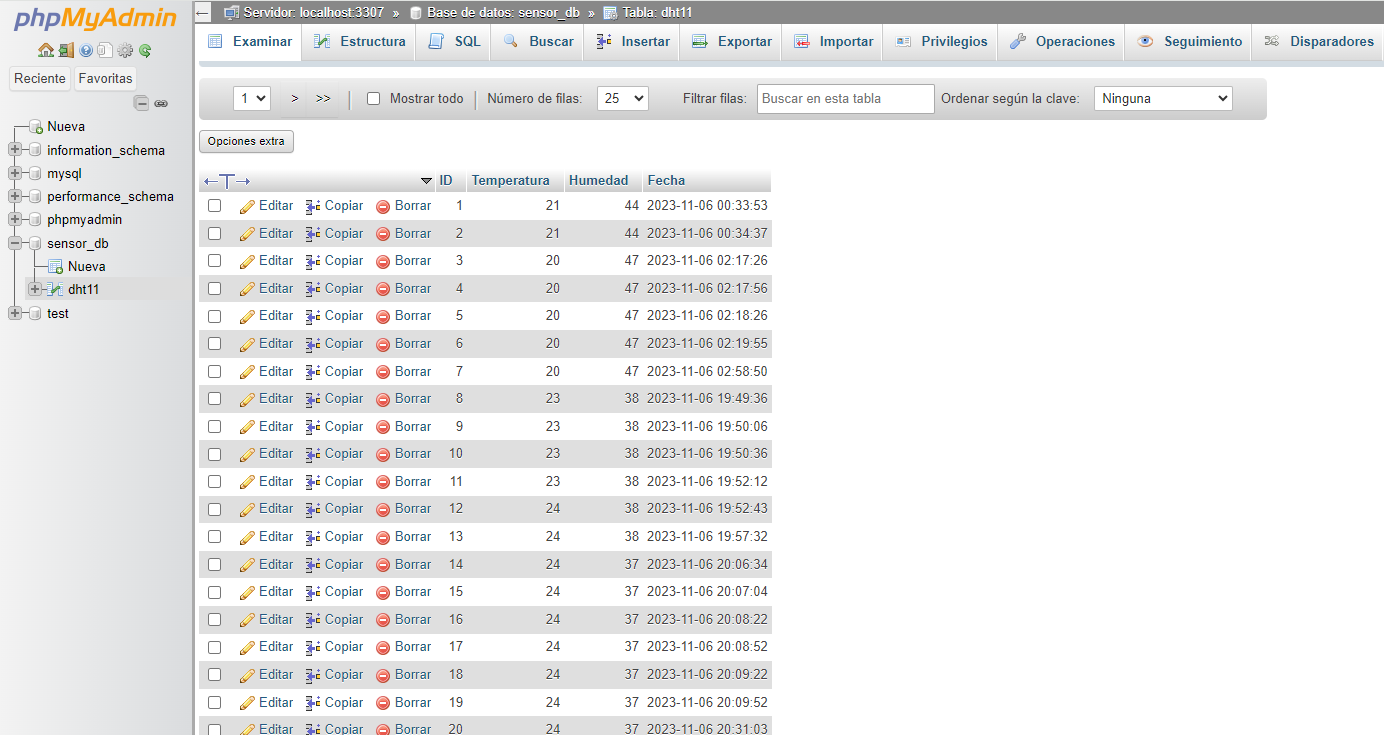
\includegraphics[scale=0.1]{images/Web/Db_compostador.png}
            
            \caption{Base de datos }
            \label{fg:pagina_web}
        \end{figure}
\clearpage

\textbf{Verificación subsistema 1}

Como se mencionó en el apartado anterior, el menú desplegado en la interfaz presenta tres opciones y para comprobar que cada una funciona de manera correcta, se realizaron varias pruebas.

Para probar el monitoreo del proceso, se ejecutaron los distintos procesos de forma aislada, es decir se programó una rutina de calentamiento durante cierto periodo de tiempo para verificar el aumento de temperatura y el registro por parte del sensor figura (\ref{fg:botones_imp1}).

\begin{figure}[h]
            \centering
            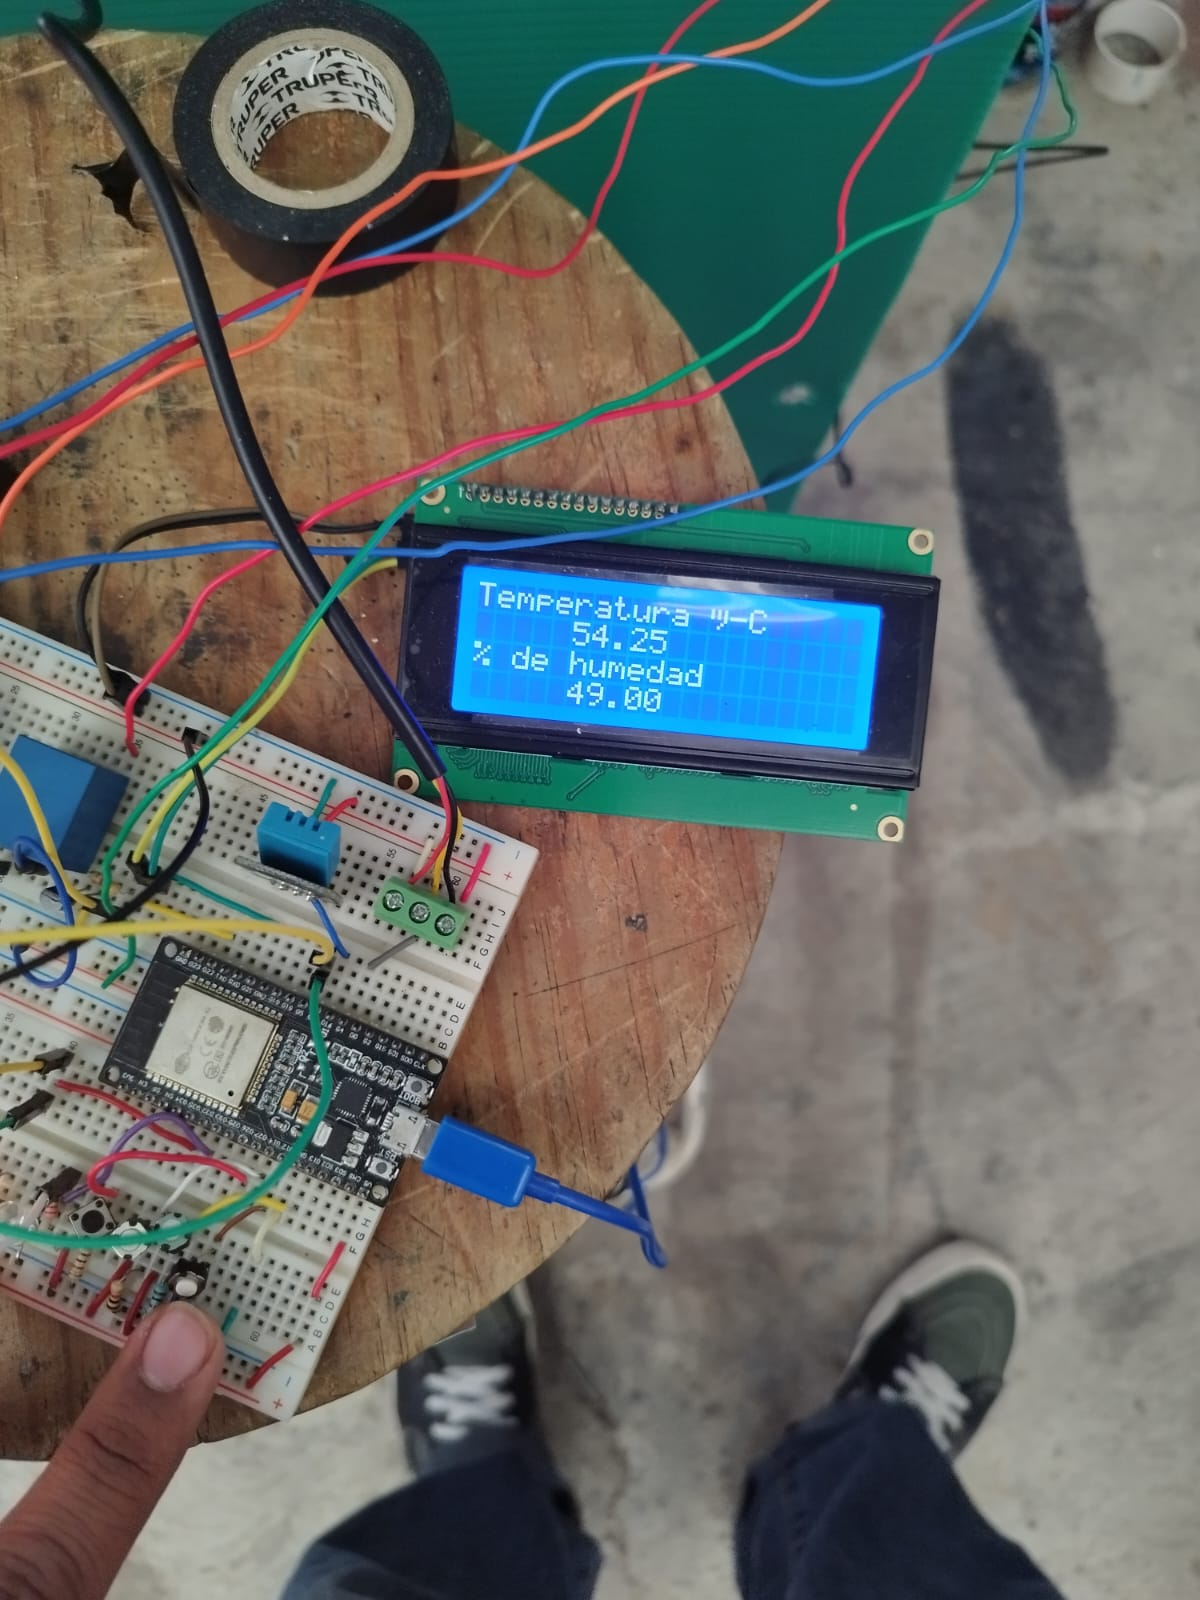
\includegraphics[scale=0.23]{images/Pruebas/Pruebas_S1/mostrar_aumento_temperatura.jpeg}
            \caption{Mostrar aumento de temperatura}
            \label{fg:botones_imp1}
\end{figure}

\clearpage

A la vez se medía el tiempo que tardaba el contenedor en calentarse, cuanto tiempo se mantenía la temperatura con el cinturón apagado y el tiempo en el que se registraba un descenso de la temperatura al interior figura (\ref{fg:botones_imp2}).

\begin{figure}[h]
            \centering
            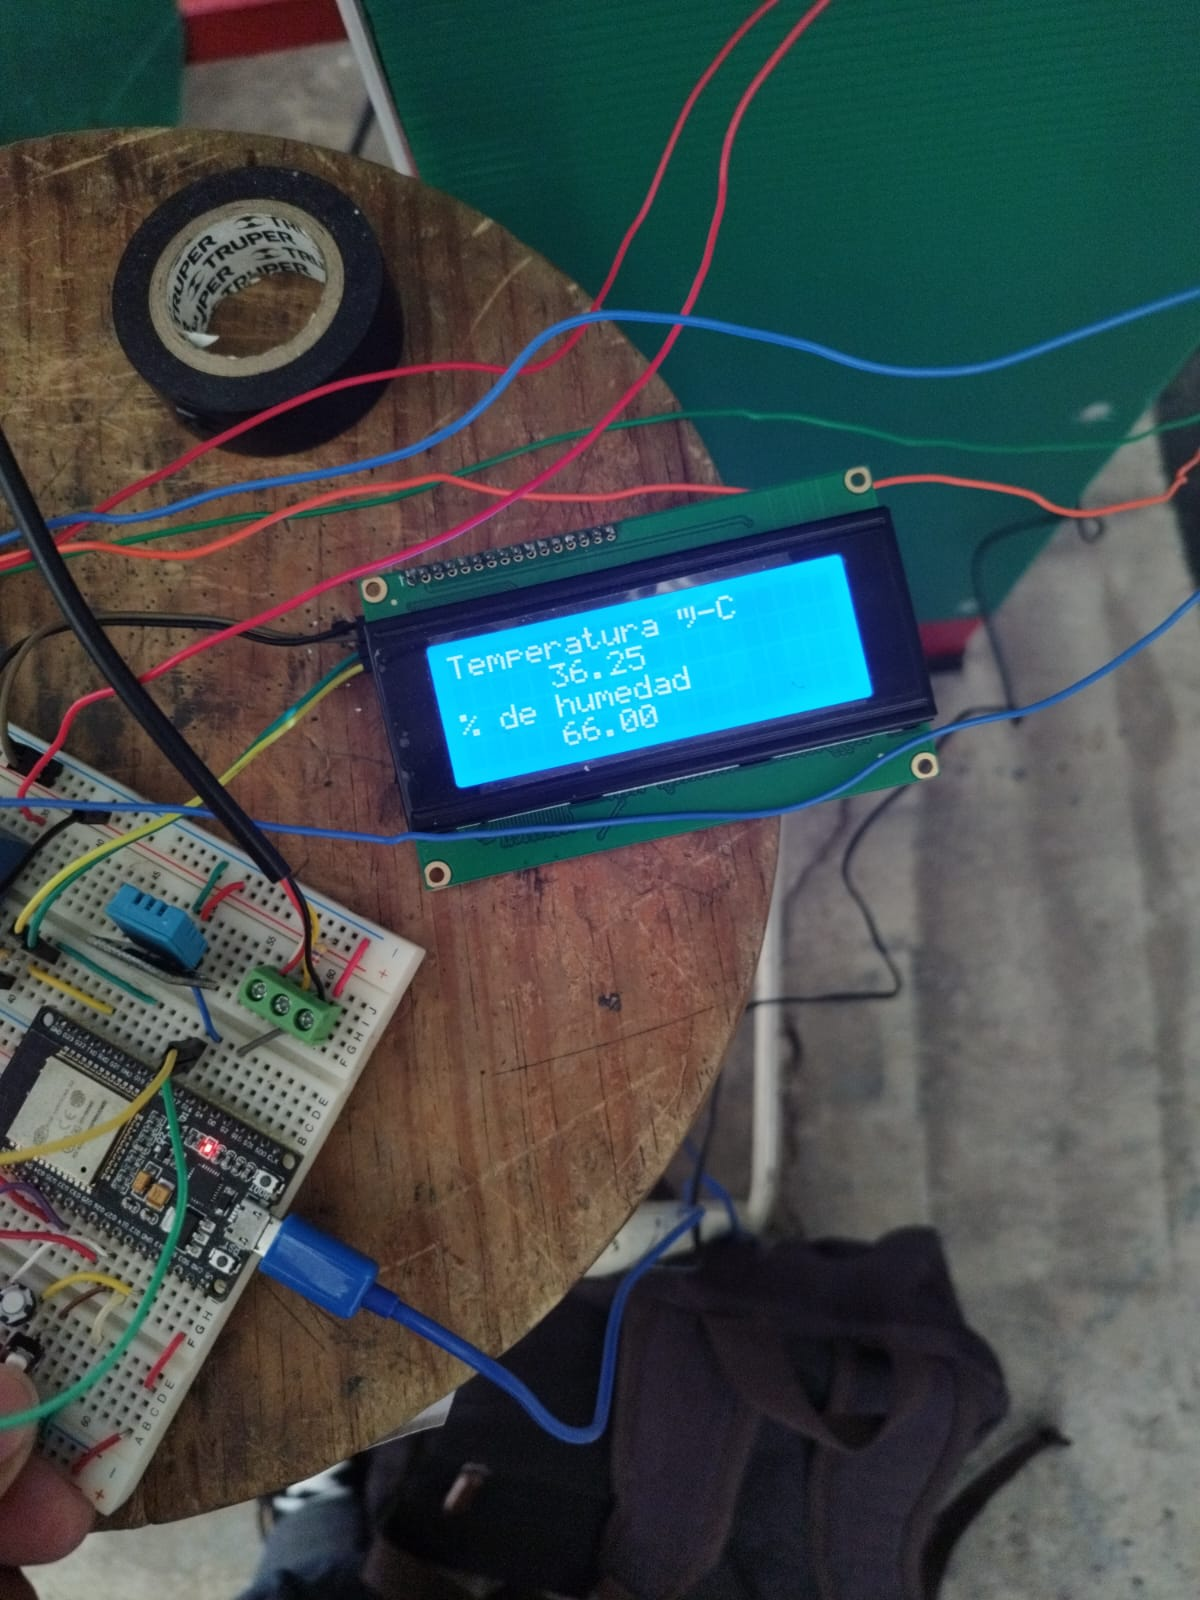
\includegraphics[scale=0.25]{images/Pruebas/Pruebas_S1/mostrar_datos.jpeg}
            \caption{Mostrar descenso de temperatura}
            \label{fg:botones_imp2}
\end{figure}

\clearpage

Para verificar el proceso, de igual manera se realizaron rutinas para corroborar que en pantalla se estuviera mostrando la etapa adecuada del compostaje figura (\ref{fg:botones_imp3}) y figura (\ref{fg:botones_imp4}).

\begin{figure}[h]
            \centering
            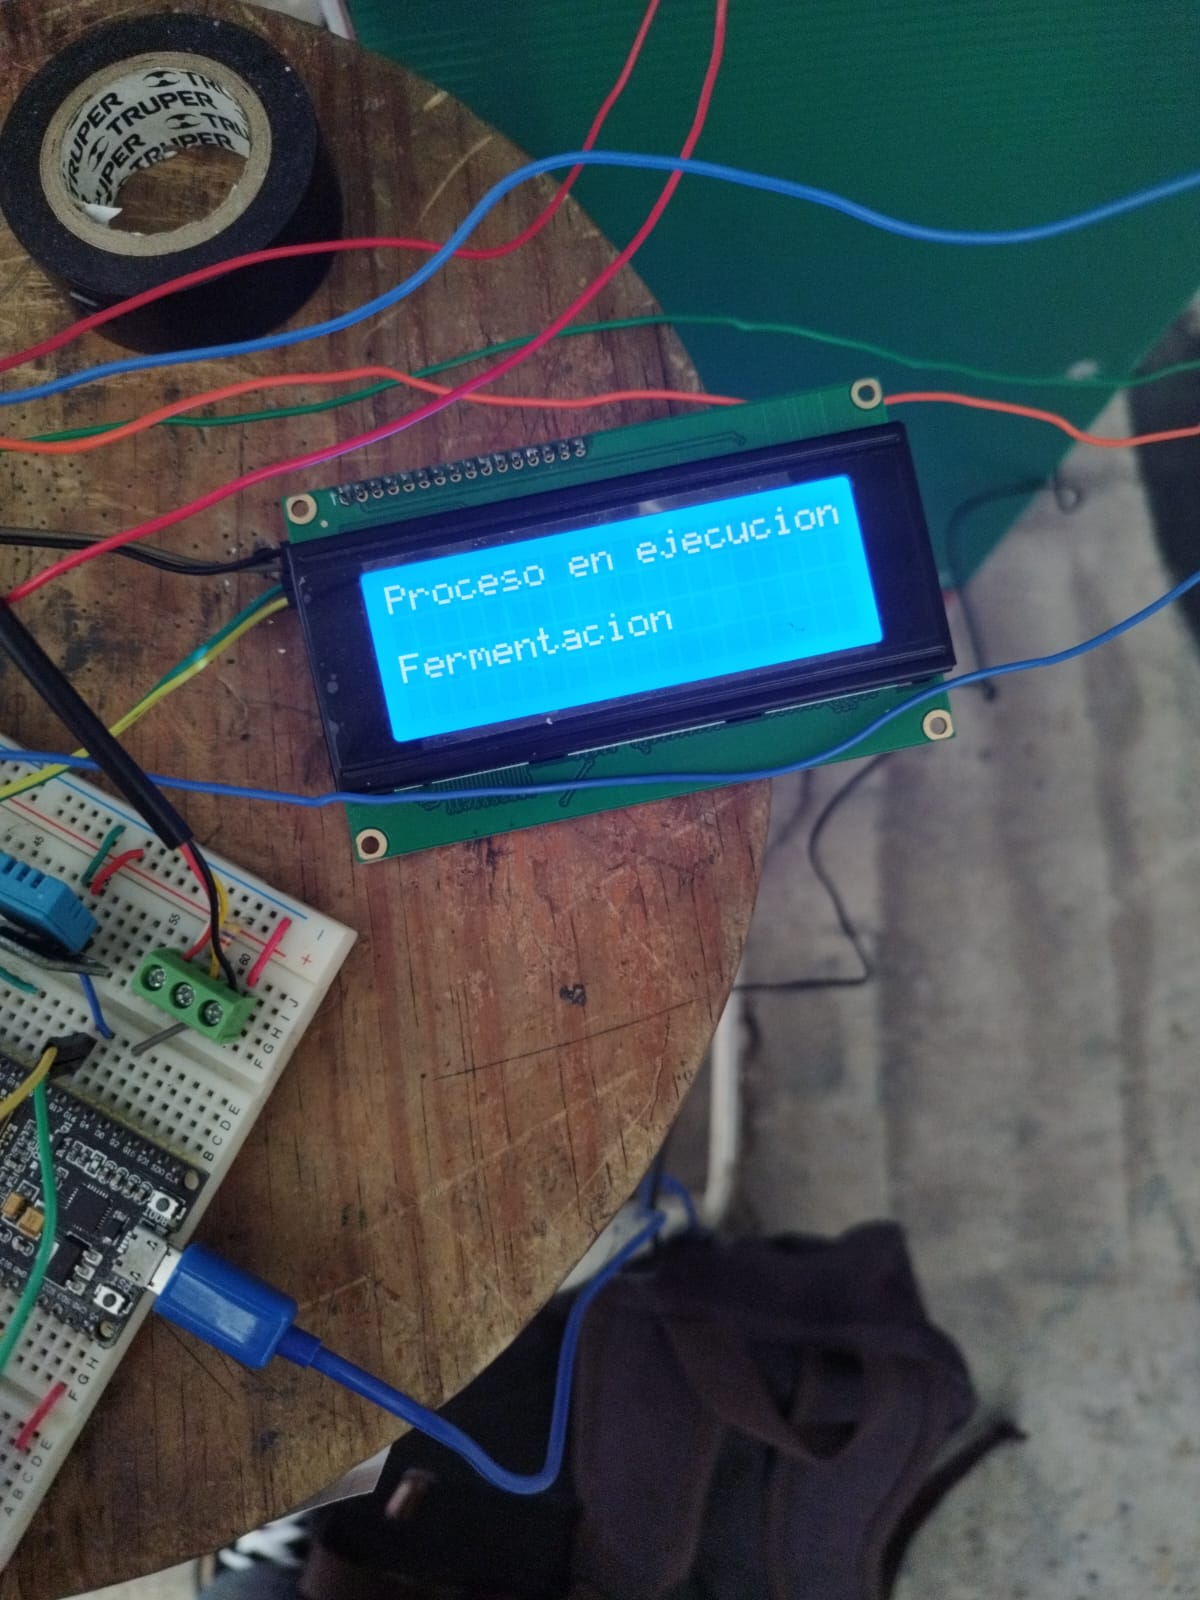
\includegraphics[scale=0.25]{images/Pruebas/Pruebas_S1/fermentacion.jpeg}
            \caption{Ejecutando fermentación}
            \label{fg:botones_imp3}
\end{figure}
\clearpage

\begin{figure}[h]
            \centering
            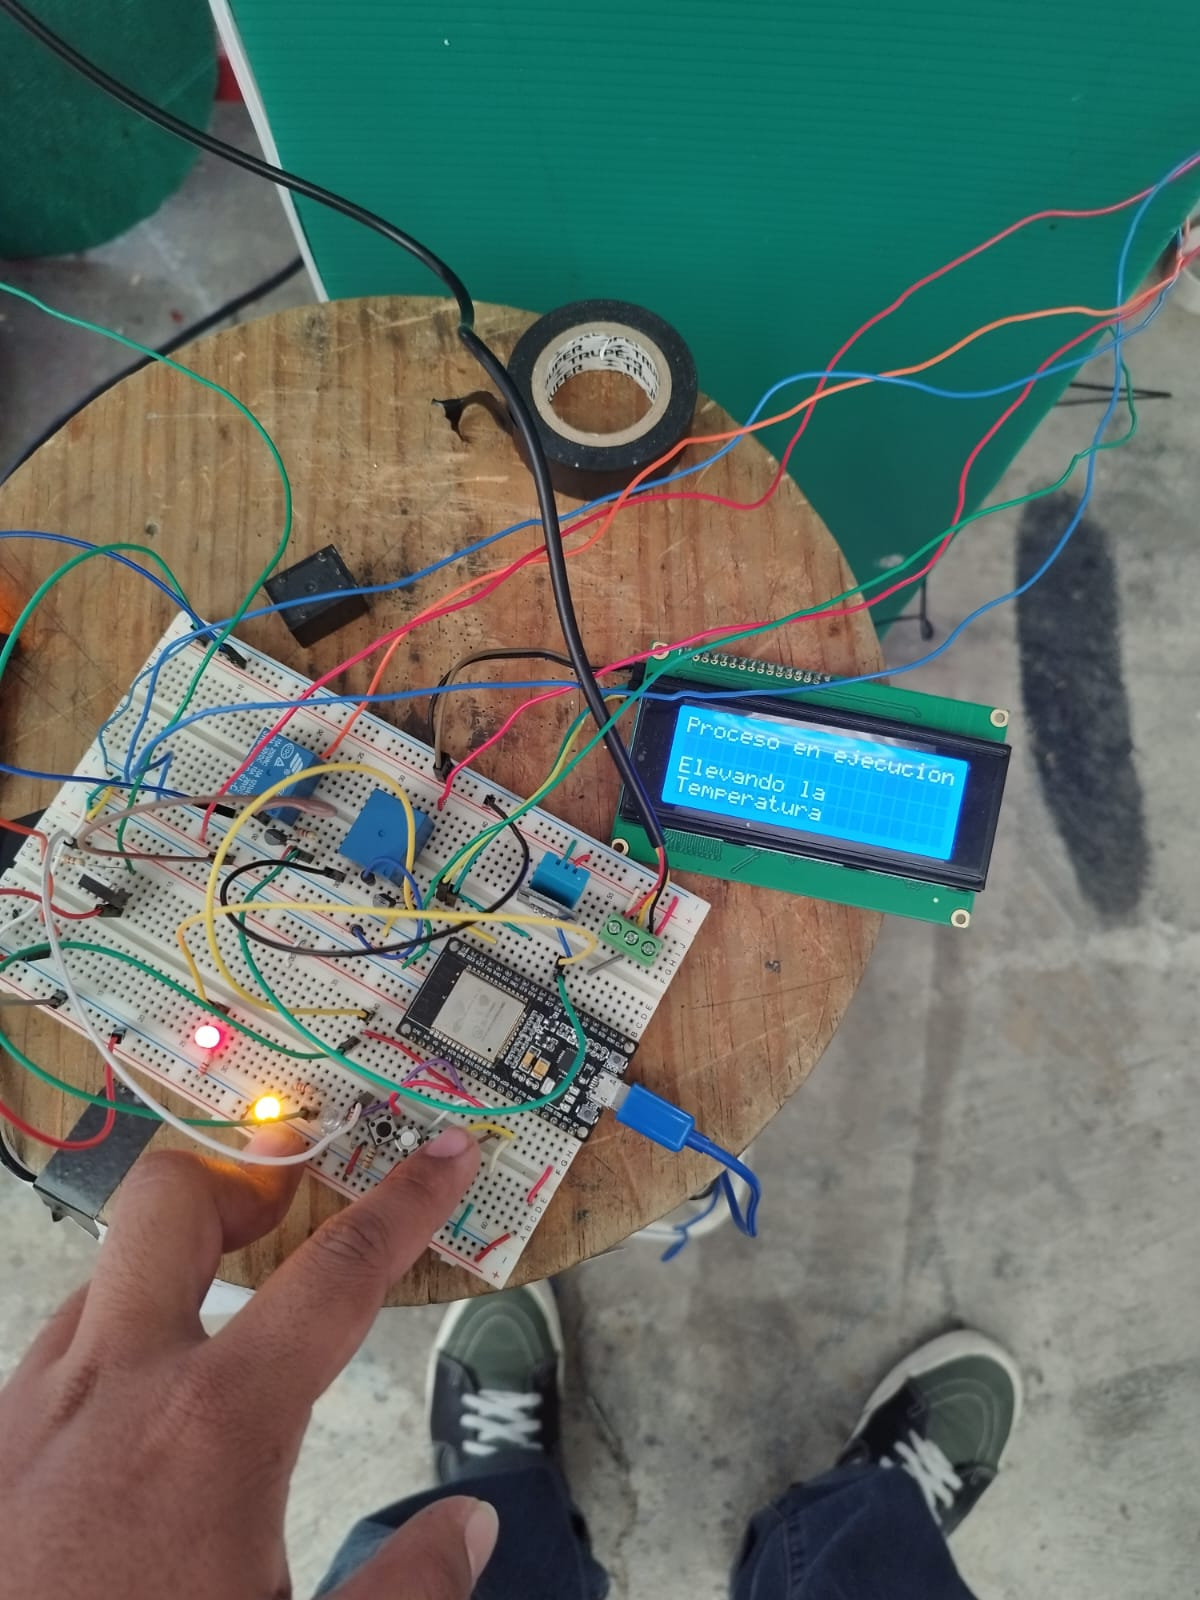
\includegraphics[scale=0.25]{images/Pruebas/Pruebas_S1/elevando_temp.jpeg}
            \caption{Ejecutando elevación de temperatura}
            \label{fg:botones_imp4}
\end{figure}

\clearpage     

Por último, para verificar que el tiempo de ejecución fuera real, se comparó la duración de ciertas rutinas con un cronómetro de celular, para comprobar que los tiempos fueran prácticamente los mismos figura (\ref{fg:botones_imp5}).

\begin{figure}[h]
            \centering
            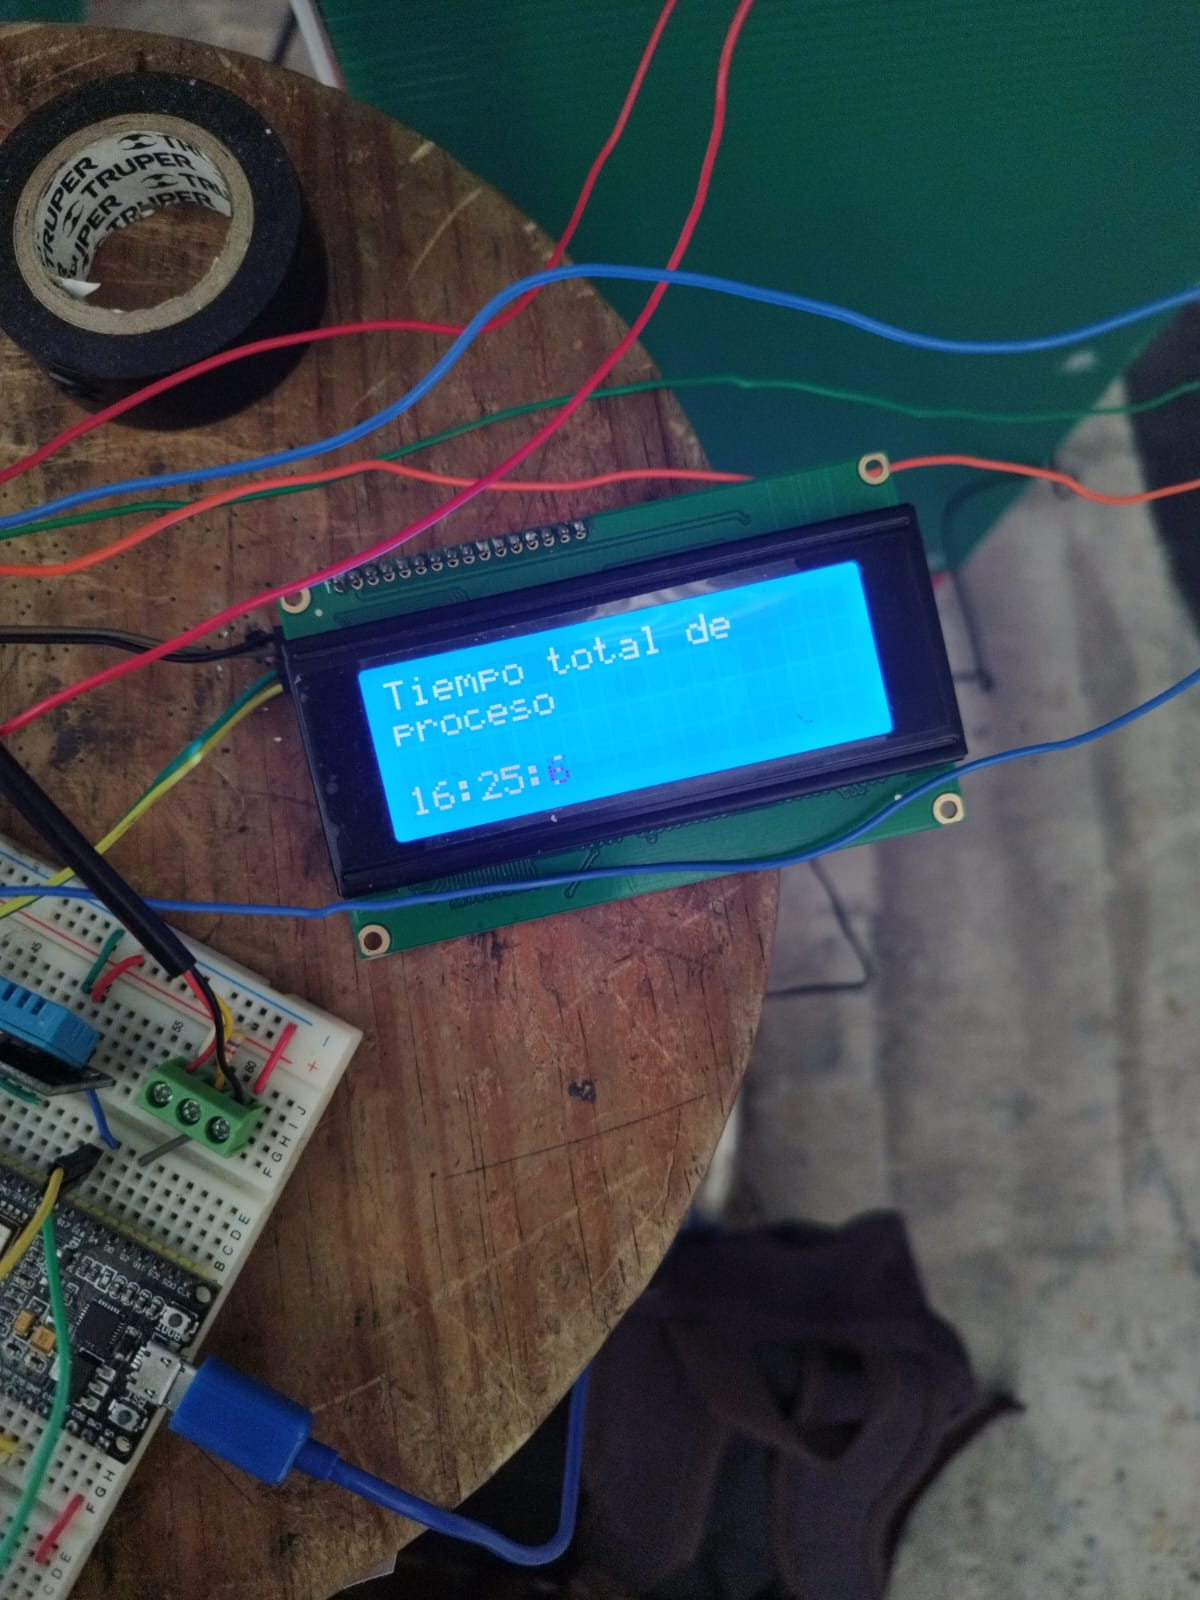
\includegraphics[scale=0.25]{images/Pruebas/Pruebas_S1/conteo_tiempo.jpeg}
            \caption{Verificación del tiempo}
            \label{fg:botones_imp5}
        \end{figure}


\clearpage




\subsection{Sistema de procesamiento de datos $S_2$}

\textbf{Implementación de los sensores y su sistemas de acondicionamiento}

Para esta parte, en la protoboard donde se ha conectado la ESP32, se han instalado los elementos necesarios para el funcionamiento de los sensores. Para el caso del sensor DS18B20, de temperatura, es necesario agregar una resistencia de 4.7 $\Omega$ entre la salida del sensor y la alimentación de 5$V$, para conectarse con el pin 4 de la ESP32, como se ve en la figura \ref{fg:cto_sensores_impl}.

\begin{figure}[h!]
            \centering
            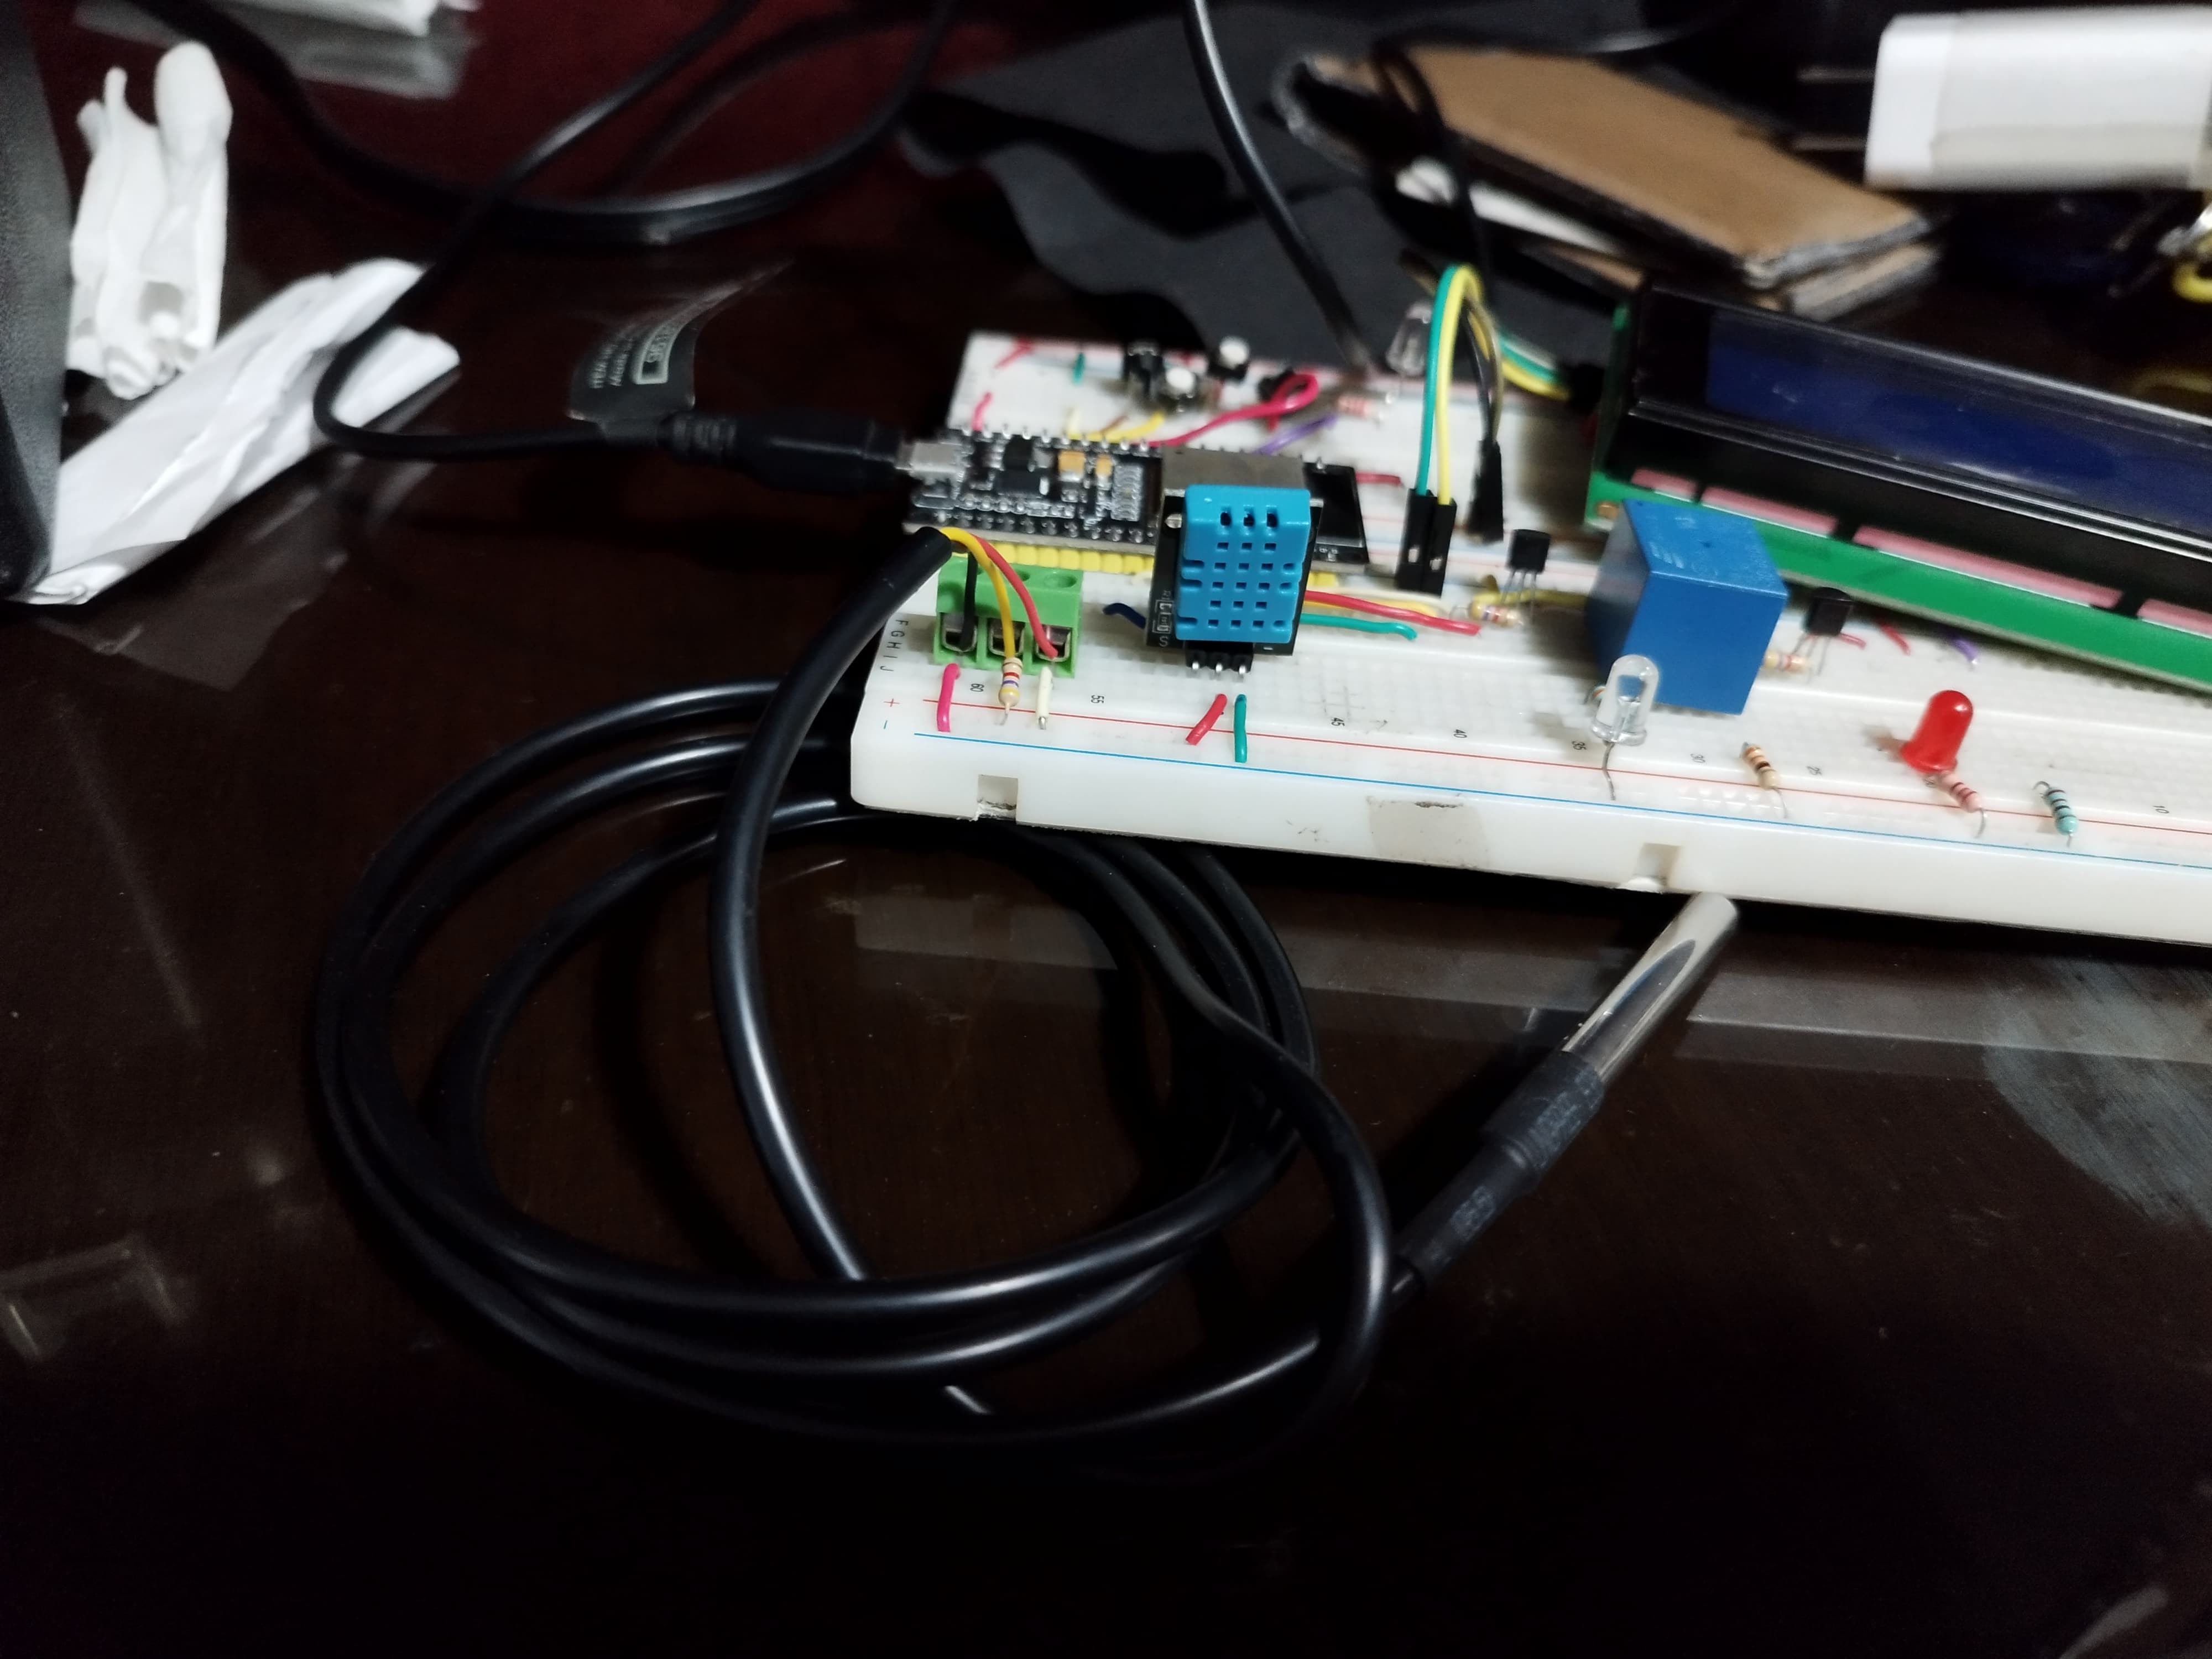
\includegraphics[scale=0.1]{images/Capitulo_Imple/S2/CTO_SEN.jpeg}
            \caption{Conexión de los sensores en la protoboard}
            \label{fg:cto_sensores_impl}
\end{figure}
\clearpage

En caso del sensor DHT11 (figura \ref{fg:DHT11_Fisico}), de humedad, no es necesario realizar alguna conexión externa, debido a que se cuenta con la versión del sensor que viene en una placa PCB, el cual presenta la resistencia de 10 $k\Omega$, por lo que se conecta la señal de lectura, directa al pin 17 de la ESP32.

\begin{figure}[h!]
            \centering
            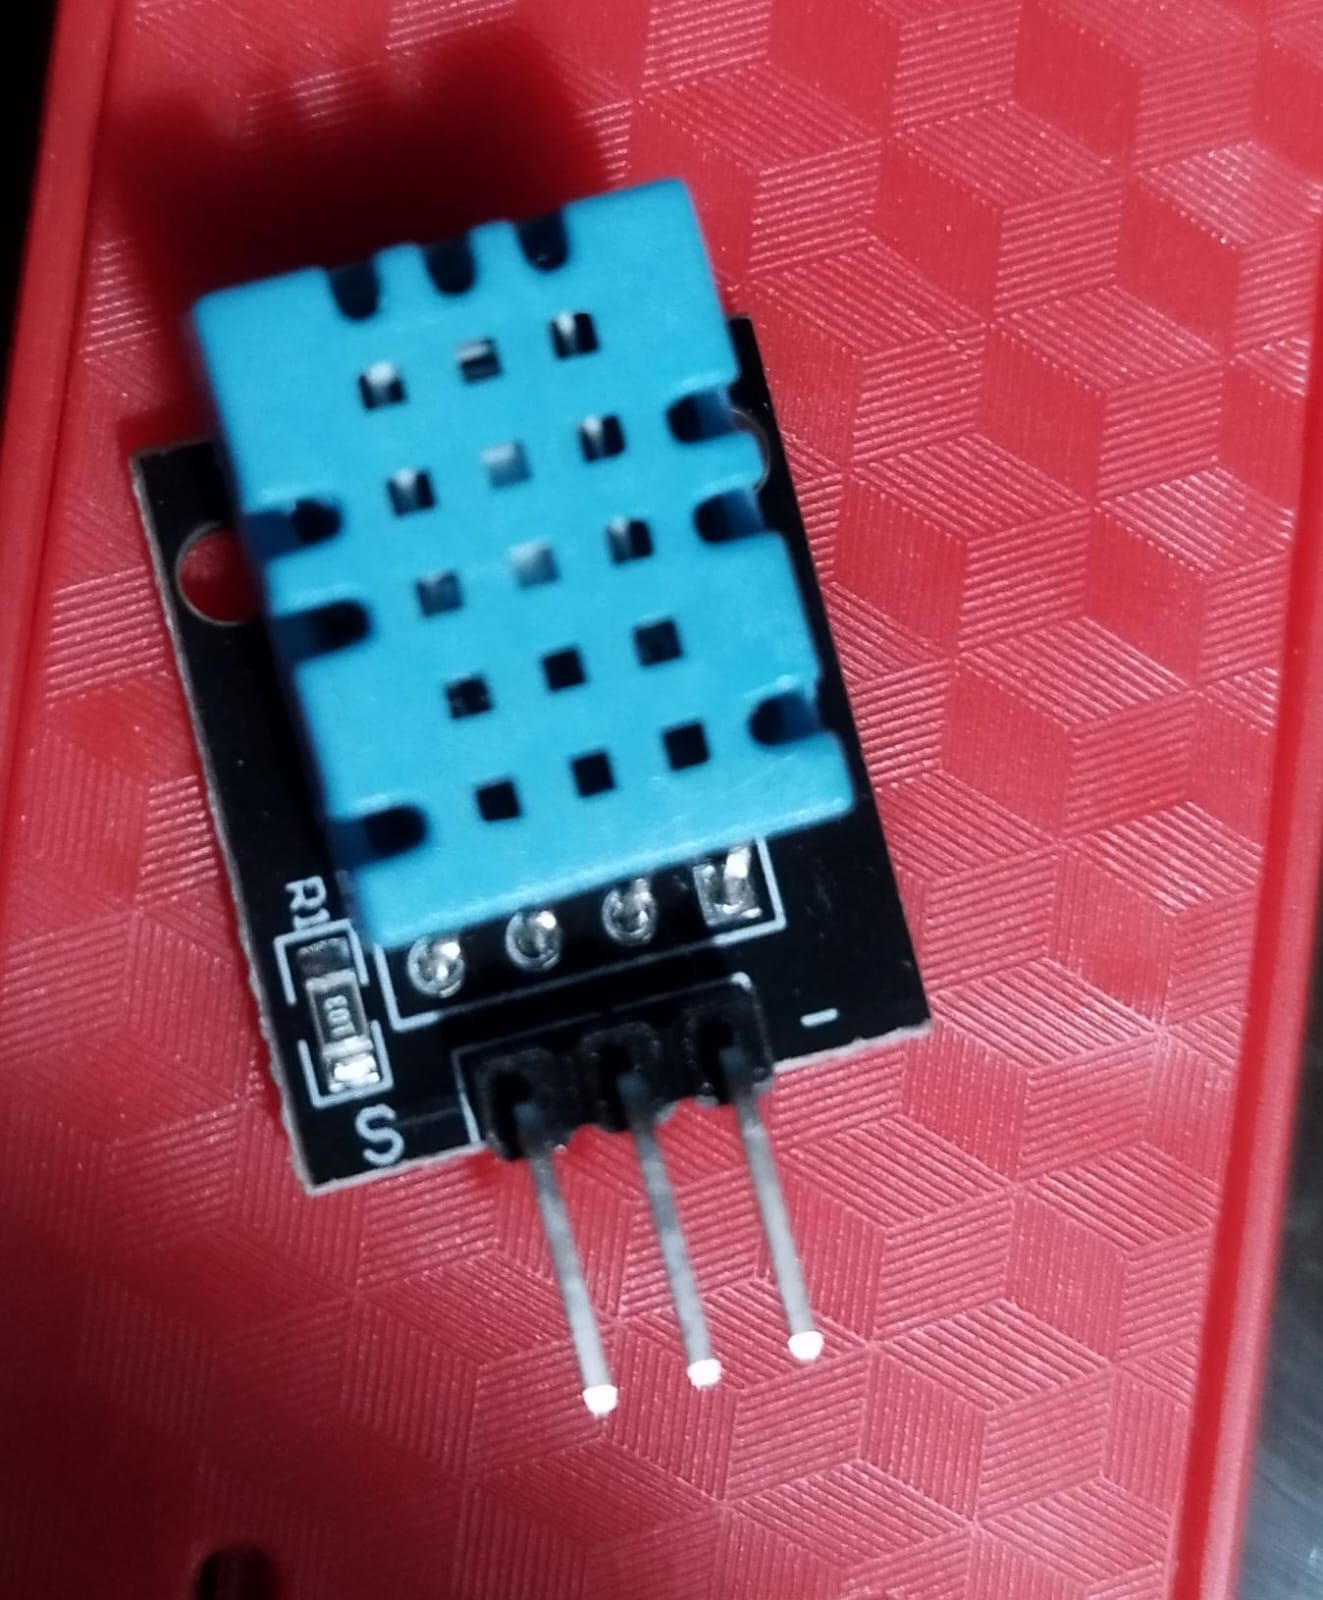
\includegraphics[scale=0.1]{images/Capitulo_Imple/S2/DHT11_FIS.jpeg}
            \caption{Sensor DHT11 que se utilizó}
            \label{fg:DHT11_Fisico}
\end{figure}

Ya conectados, se integran al programa utilizando la biblioteca "DHT sensor library" de Adafruit, "DallasTemperature" de Miles Burton y "OneWire" de Jim Studt para utilizar los acondicionamientos digitales dentro del microprocesador. De esta manera, se leen los valores de las variables físicas y puedan ser mostrados al usuario por medio de la LCD, como se ve en la figura. \ref{fg:cto_senso_funcionando}.

\begin{figure}[h]
            \centering
            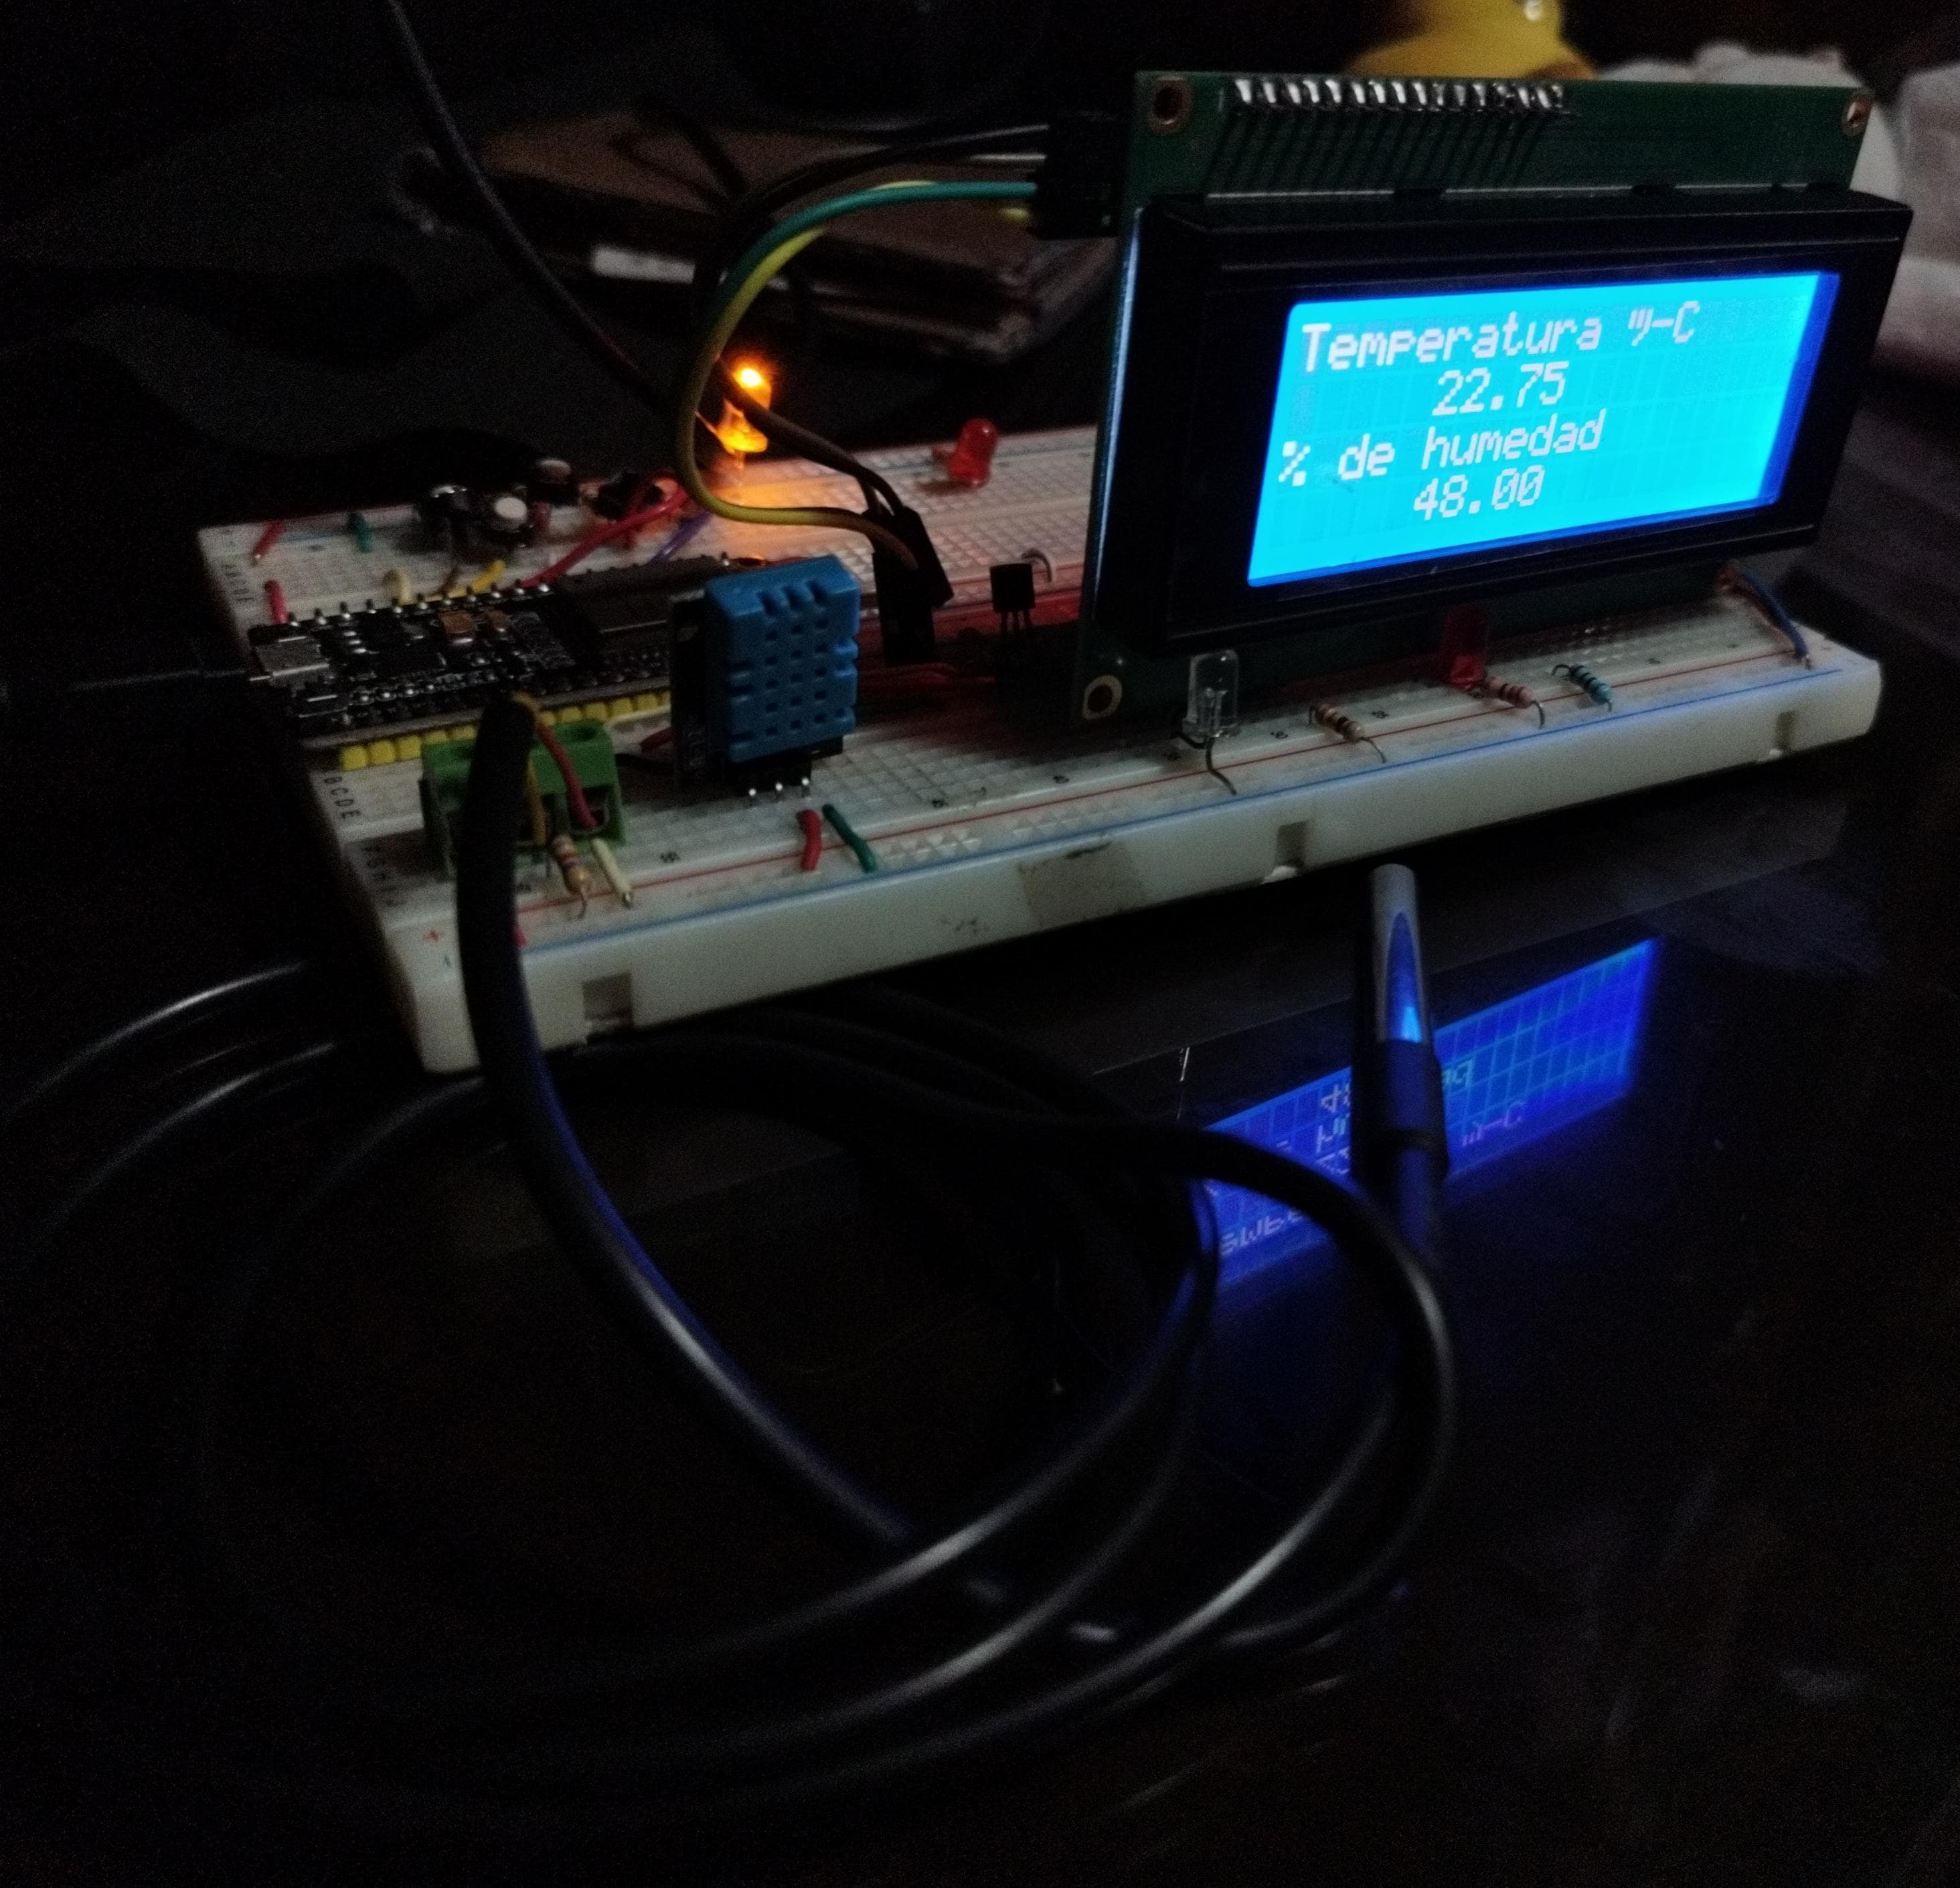
\includegraphics[scale=0.15]{images/Capitulo_Imple/S2/SEN_FUNCIONANDO.jpeg}
            \caption{Circuito de prueba de la interfaz}
            \label{fg:cto_senso_funcionando}
        \end{figure}
\clearpage

%\subsection{Validación  $S_2$}



\newpage
\subsection{Sistema de energía $S_3$}

\textbf{Cálculos energéticos del sistema}

En esta parte se realizan los cálculos para determinar cuánta energía eléctrica es capaz de consumir el dispositivo y, de esta manera, realizar una aproximación del costo económico que representaría.

\textbf{Calculo máximo de energía.}

En este cálculo se tiene en cuenta que todos los subsistemas están encendidos al mismo tiempo; si bien es una opción poco probable, con este valor se puede determinar qué tipo de instalación se requiere para ponerlo en marcha.

Para cada uno de los elementos eléctricos del sistema mecatrónico,se tienen los siguientes valores de potencia eléctrica (Tabla \ref{tab:Electrical_values}).


\begin{table}
    \centering
\caption{Valores de potencia de los elementos eléctricos del sistema}
\label{tab:Electrical_values}
    \begin{tabular}{|m{2.5cm}|m{2.5cm}|m{2.5cm} |m{2.5cm}|} \hline 
         Elemento&  Potencia Activa nominal (W)&Factor de Potencia FS &Potencia aparente (VA)\\ \hline 
         Motor de trituración&  1397&1.35 &1034.815\\ \hline 
         Motor de aireación&  180&1.35 &133.333\\ \hline 
         Circuito electrónico&  20&1 &20\\ \hline 
         Resistencia eléctrica&  1000&1 &1000 \\ \hline 
         Ventilador&  12&1 &12\\ \hline 
         Fuente de 24 V&  120&1 &120 \\\hline
    \end{tabular}
    
    
\end{table}

Para encontrar la corriente máxima $I_{MAX}$ que será necesaria para alimentar el circuito, es necesario encontrar la potencia aparente total del sistema $S_T$  y esta es dividida por el valor de la tensión de alimentación $V$. Entonces el valor obtenido es:

\begin{equation*}
    I_{MAX} = \frac{S_T}{V} = \frac{2320.148}{127} = 18.269 A
\end{equation*}
De tal manera que si todos los elementos del sistema están encendidos al mismo tiempo, esta será la corriente consumida del sistema.

\textbf{Cálculo por cada proceso del sistema}

Para esta parte, se hace el cálculo de cada uno de los procesos por separado, considerando únicamente, los subsistemas que trabajan al mismo tiempo en determinada parte del proceso.

\textit{Proceso de fermentación}

En esta parte del proceso, únicamente se tiene en cuenta el funcionamiento del circuito electrónico, para mantener el registro de los sensores, así como el funcionamiento de la interfaz humano-máquina; también se tiene activa la fuente de 24 V. Este proceso está programado para llevarse a cabo por 2 horas y media, por lo que la energía consumida en este periodo de tiempo está expresada en la tabla. \ref{tab:fermentacion_elec}.


\begin{table}
    \centering
\caption{Consumo energético en fermentación}
\label{tab:fermentacion_elec}
    \begin{tabular}{|c|c|} \hline 
         Elemento&  Potencia consumida (KW/h)\\ \hline 
         Circuito electronico&  0.050\\ \hline 
         Fuente de 24 V&  0.300\\\hline
    \end{tabular}
    
    
\end{table}

Por lo que al realizar la suma de la potencia consumida en este periodo de tiempo, da el siguiente valor:

\begin{equation*}
    P_{fer} = 0.350   KWh
\end{equation*}

\textit{Proceso de aireación}

Para este proceso, se requiere del subsistema de ventilación y el sistema de rotación del eje de aireación, también del sistema electrónico principal. Esta tarea se va a ejecutar por un ciclo de 10 minutos, por lo que el consumo de energía en esta parte del proceso está descrito en la tabla. \ref{tab:Airo_compo}.

\begin{table}
    \centering
\caption{Consumo energético en aireación}
\label{tab:Airo_compo}
    \begin{tabular}{|c|c|} \hline 
         Elemento&  Potencia consumida (KWh)\\ \hline 
         Circuito electrónico&  0.003\\ \hline 
 Motor de aireación&0.030\\ \hline 
 Ventilador&0.002\\ \hline 
         Fuente de 24 V&  0.020\\\hline
    \end{tabular}
    
    
\end{table}

Por lo que al realizar la suma de la potencia consumida en este periodo de tiempo, da el siguiente valor.

\begin{equation*}
    P_{fer} = 0.0.055   KWh
\end{equation*}

\textit{Proceso de regulación de temperatura}

Para esta parte, es necesario tener encendida la resistencia eléctrica, así como el eje de aireación y los sistemas electrónicos del sistema. Este proceso se lleva a cabo en un tiempo promedio de 20 minutos por cada hora de proceso, dependiendo de la temperatura ambiental y la pérdida de calor del contenedor. El consumo energético de este proceso está descrito en la tabla. \ref{tab:Temp_elec}.

\begin{table}
    \centering
\caption{Consumo energético cuando se eleva la temperatura}
\label{tab:Temp_elec}
    \begin{tabular}{|c|c|} \hline 
         Elemento&  Potencia consumida (KW/h)\\ \hline 
         Circuito electrónico&  0.008\\ \hline 
 Motor aireación&0.075\\ \hline 
 Resistencia eléctrica&0.417\\ \hline 
         Fuente de 24 V&  0.050\\\hline
    \end{tabular}
    
    
\end{table}

Por lo que al realizar la suma de la potencia consumida en este ciclo, se tiene el siguiente resultado.

\begin{equation*}
    P_{fer} = 0.550   KWh
\end{equation*}

\textit{Proceso de trituración}

Para este proceso, es necesario tener encendido el motor de trituración y la electrónica del sistema. Para llevar a cabo la molienda de 15 kg de materia, fue necesario mantener encendido el sistema por una hora y media, por lo que el consumo energético de este proceso está descrito en la tabla. \ref{tab:Tritu_cons}.

\begin{table}
    \centering
\caption{Consumo energético del sistema de trituración}
\label{tab:Tritu_cons}
    \begin{tabular}{|c|c|} \hline 
         Elemento&  Potencia consumida (KW/h)\\ \hline 
         Motor de trituración&  2.096\\ \hline 
         Circuito electrónico&0.040\\ \hline 
         Fuente de 24 V&  0.240\\\hline
    \end{tabular}
    
    
\end{table}

Por lo que al realizar la suma de la potencia consumida en este ciclo, se tiene el siguiente resultado.

\begin{equation*}
    P_{fer} = 2.376   KWh
\end{equation*}

\textbf{Cálculo por el total del proceso}

Para esta parte, se hace el cálculo estimado del consumo de energía eléctrica por un ciclo de 72 horas, donde los datos que se toman en cuenta, están resumidos en la tabla \ref{tab:Electrical_values_total}

\begin{table}
    \centering
\caption{Consumo total de los elementos eléctricos del sistema}
\label{tab:Electrical_values_total}
    \begin{tabular}{|m{2.5cm}|m{2.5cm}|m{2.5cm}|m{2.5cm}|} \hline 
         Elemento&  Potencia activa nominal (W)&Tiempo encendido (hr)&Energia consumid (KWh)\\ \hline 
         Motor de trituración&  1397&1.5&2.096\\ \hline 
         Motor de aireación&  180&24.5&4.410\\ \hline 
         Circuito electrónico&  20&72&1.440\\ \hline 
         Resistencia eléctrica&  1000&20&20\\ \hline 
         Ventilador&  12&6&0.072\\ \hline 
         Fuente 24 V&  120&72&8.640\\ \hline
    \end{tabular}
    
    
\end{table}

Por lo que sumando todos los valores de la ultima columna, el consumo total de energía del dispositivo es representado de la siguiente forma.

\begin{equation*}
    P_{total} = 36.658 KWh
\end{equation*}

Tomando en cuenta el costo de la luz en tarifa domestica de Enero 2024, emitido por la Comisión Federal de Electricidad, donde el kilowatt de energía cuesta \$ 1.005 MXN, el costo de la energía consumida en el proceso total es de \$ 36.840 MXN.

\clearpage

%\textbf{Verificación subsistema 3}



\newpage
\subsection{Sistema de trituración $S_4$}

\textbf{Implementación del molino de carne }

Para realizar la operación del triturado del sistema, se determinó utilizar un molino de carne. Para implementarlo, fue necesario lavar el dispositivo para retirarle la cubierta de estaño que traía de fábrica, ya que esta capa se suele caer por sí sola a lo largo del tiempo, pero puede ser perjudicial para la generación del compost.

Una vez lavado, fue necesario realizarle un rectificado a las patas del triturador con ayuda de un esmeril. De esta manera, se aseguró de que se tenga una mayor superficie de contacto y, por ende, evitar vibraciones al momento de ser atornillado a la estructura.

También se colocó una polea de 14 pulgadas de diámetro a la entrada del eje, para recibir el impulso que haga rotar al tornillo sin fin por medio de una banda.\\
\clearpage

\textbf{Implementación de la motorización del sistema de trituración.}

Esta parte se agregó al sistema con el fin de facilitarle al usuario la trituración de los residuos orgánicos, buscando que el sistema sea amigable con el usuario.

Para este fin, se utilizó un motor de corriente alterna que fue extraído de una lavadora de 16 kg. Al ser un motor muy potente que gira a una velocidad de 1450 rpm, se propuso utilizar un dimmer de 400 $W$ para disminuir su velocidad angular. Además de emplear un juego de poleas para obtener una velocidad de 207 rpm a la entrada del triturador.

El control de la velocidad en este caso es muy importante, debido a que, si el tornillo sin fin del triturador gira a la misma velocidad que el motor, puede provocar daños a todo el molino. Asimismo, la generación de vibraciones podría deformar la estructura o dañar componentes a largo plazo.

Este motor se activa de manera manual, gracias a una botonera que está en un costado de la estructura. Es así que el control de la trituración está en manos del usuario, por lo que no depende de los demás sistemas para funcionar y sigue siendo un sistema semiautomático que requiere de un operador para realizar algunas tareas.
 
A la salida del triturador, se colocó una tubería de PVC con la que se encaminan los desechos hacia el interior del contenedor para su procesamiento. Por lo que el sistema de entrada de la materia orgánica se aprecia en la figura. (\ref{fg:sist_tritura_fisico}).

\begin{figure}[h]
            \centering
            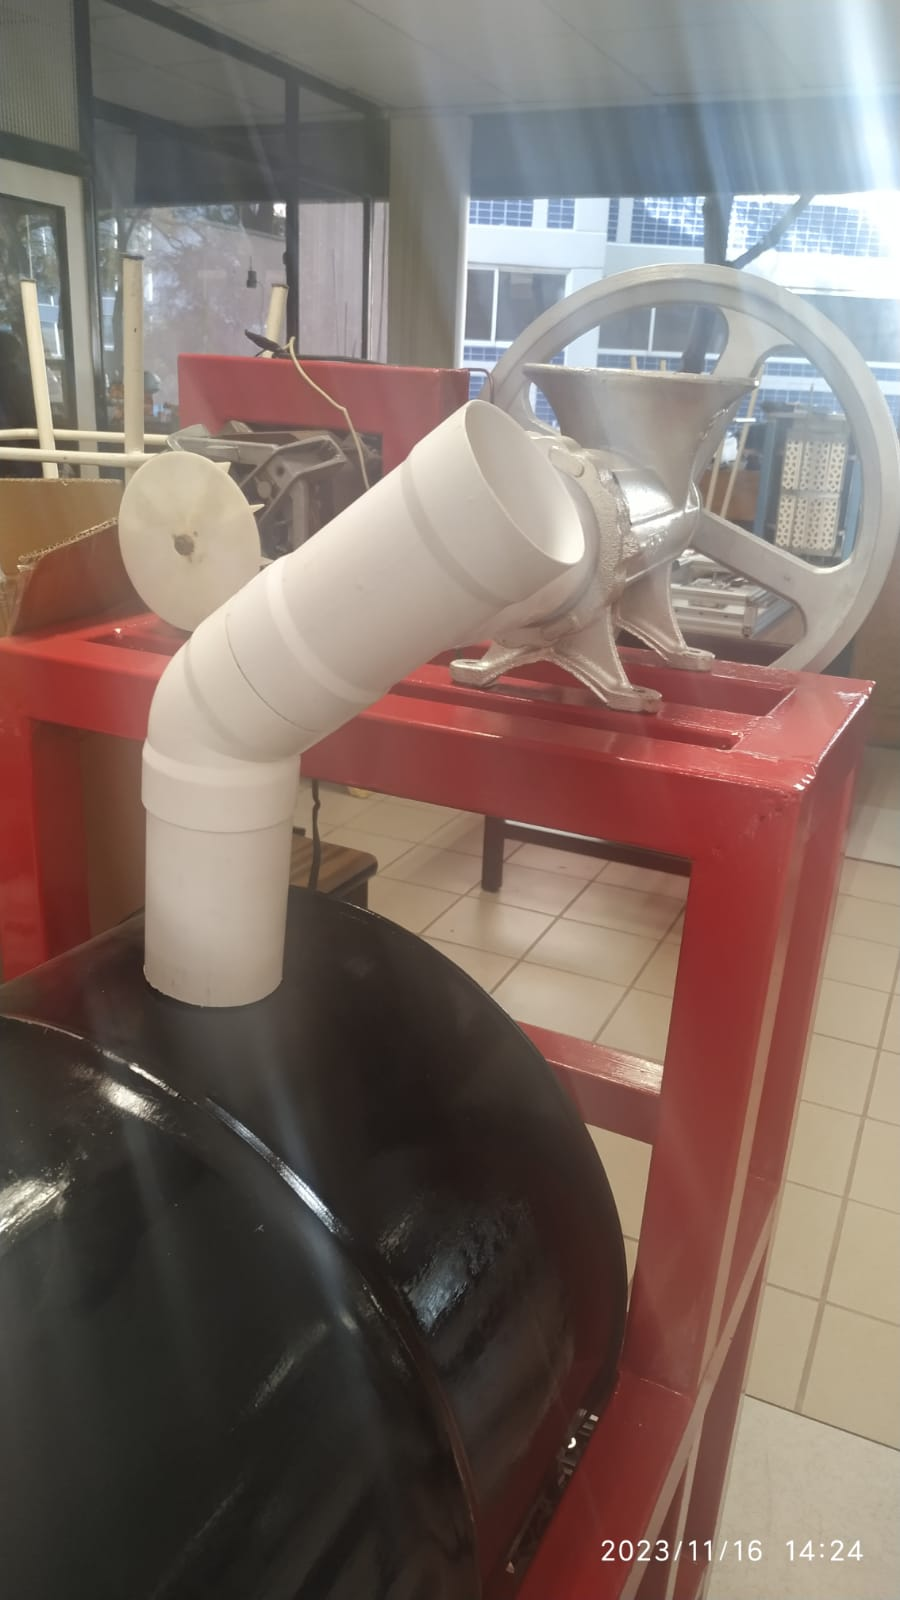
\includegraphics[scale=0.3]{images/Capitulo_Imple/S4/trituracion.jpeg}
            \caption{Sistema de trituración montado}
            \label{fg:sist_tritura_fisico}
\end{figure}

\clearpage

\textbf{Verificación subsistema 4}

Se configuró el dimmer con el objetivo de reducir la velocidad del motor de trituración. Sin embargo, durante su implementación se presentó un imprevisto, ya que la disminución del voltaje de alimentación del motor provocó que la corriente de arranque fuera demasiado elevada, ocasionando que el fusible de protección del dimmer se quemara continuamente. Debido a esto, finalmente se optó por eliminar el uso del dimmer.

Para verificar el funcionamiento del sistema de trituración, se realizaron pruebas con diversos tipos de desechos orgánicos. En la primera prueba, se utilizaron hojas de lechuga, tallos de cebollas, cáscaras de melón, trozos y cáscaras de zanahoria, así como trozos de papa.

En esta primera prueba, los trozos de papa fueron triturados en su totalidad, sin ningún tipo de inconveniente, a diferencia de los trozos de zanahoria, que, por ser de un tamaño aproximado de 5 cm de largo por 1.5 cm de ancho, atascaron la salida del molino, impidiendo la expulsión de la materia y frenando en seco el motor. (Figura \ref{fg:Atasco tritu}).

 \begin{figure}[h]
            \centering
            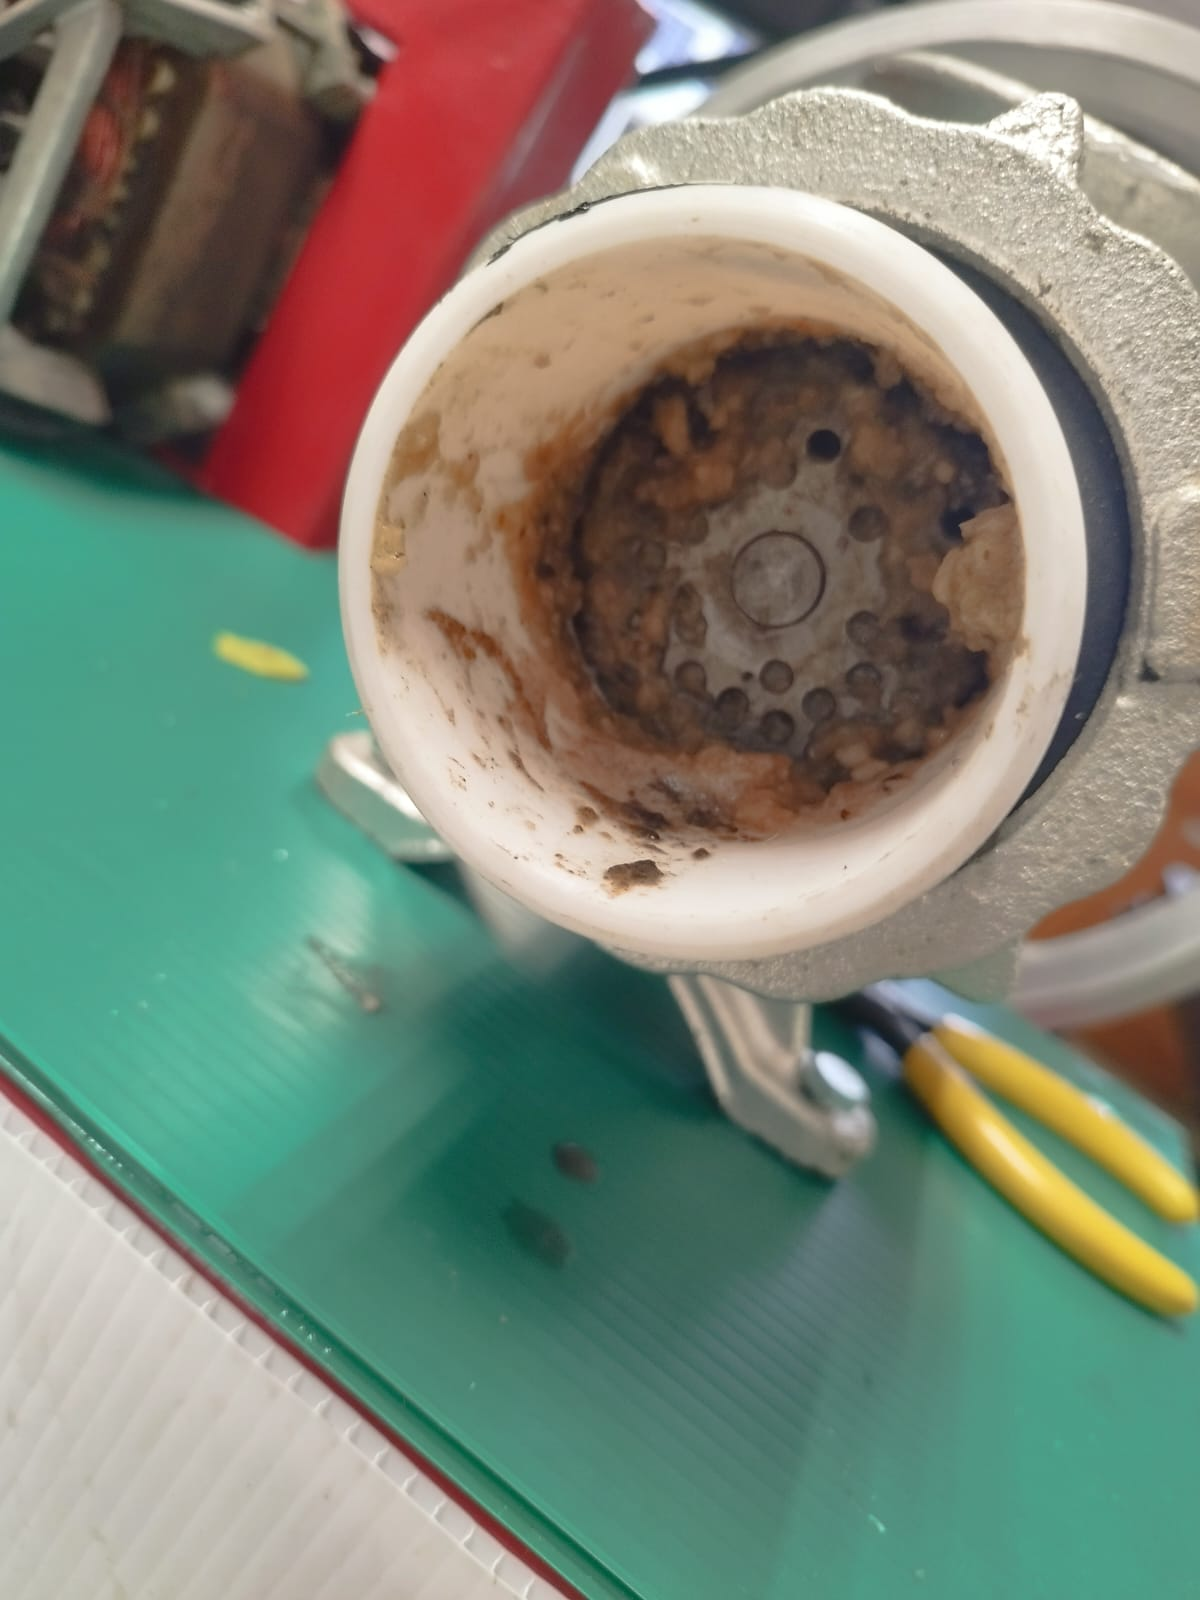
\includegraphics[scale=0.15]{images/Capitulo_Imple/S7/atorado.jpeg}
            \caption{Triturador atascado}
            \label{fg:Atasco tritu}
 \end{figure}
 
Para el caso de las hojas de lechuga, los tallos de cebollas, las cáscaras de zanahoria y melón, el sistema de trituración no era eficiente. Debido a que son elementos delgados y largos que se quedan atrapados alrededor del tornillo sin fin o en las paredes del molino.

El resultado de esta prueba fue de ayuda para delimitar el tamaño de los residuos a la entrada de la trituración. Estos deben estar en un rango de 1 a 3 cm de largo por 1 a 3 cm de ancho. Tampoco se le deben introducir tallos enteros ni cáscaras.
 
Para la segunda prueba de trituración, se utilizaron residuos de papa, zanahoria, sandía, melón y jícama. Estos elementos fueron previamente picados para cumplir con el requerimiento de entrada.

Con las muestras picadas, se procedió a introducir los desechos al triturador. Esto se hizo de forma lenta para evitar que se atascaran.

Este proceso llevó a mejores resultados, moler todos los residuos provoco un par de pequeños atascos, sin embargo a diferencia del primer experimento no generó más problemas.

De esta manera, se obtuvo una materia molida a través de un cedazo con aberturas de 3 mm (Figura \ref{fg:Mat tritu}), por lo que la materia se comenzó a almacenar dentro del contenedor.

 \begin{figure}[h]
            \centering
            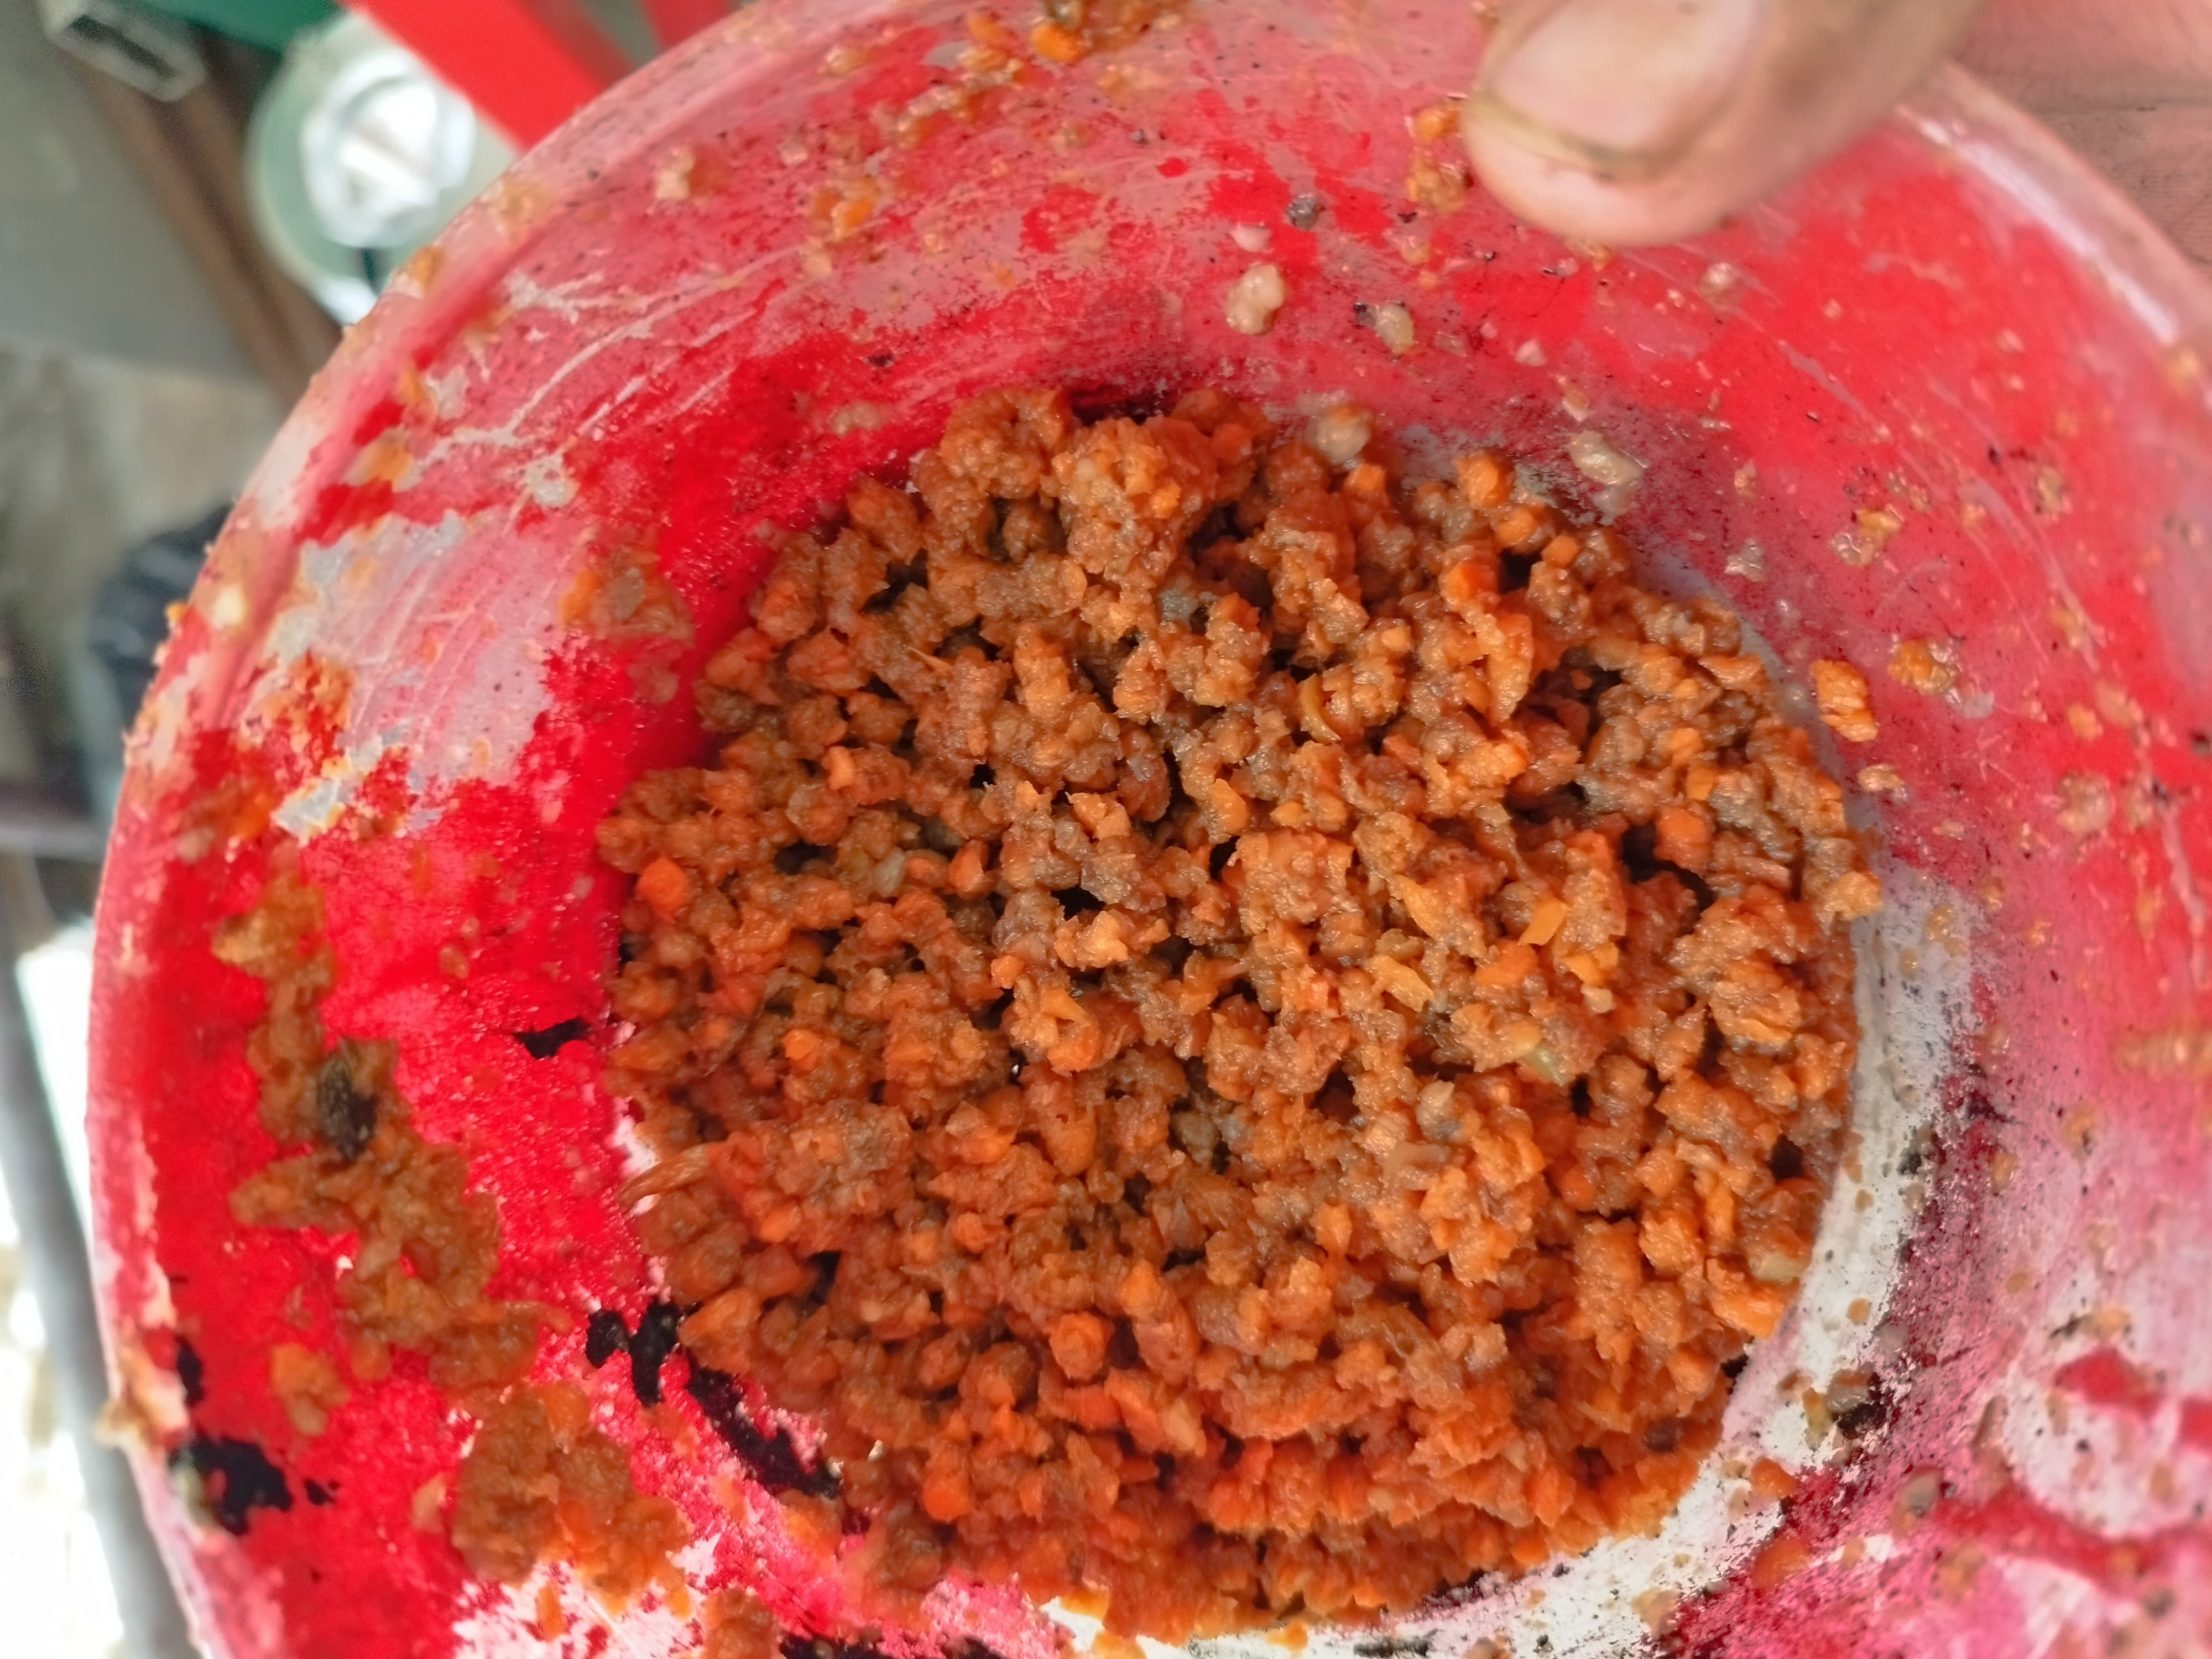
\includegraphics[scale=0.073]{images/Capitulo_Imple/S7/triturado.jpeg}
            \caption{Materia recién salida del triturador}
            \label{fg:Mat tritu}
 \end{figure}
 
 \clearpage
 
Por otro lado, estas pruebas permitieron notar que el adaptador que conecta al triturador con la estructura de PVC también contribuía con el atascamiento de la materia triturada, ya que el diámetro interior no era del tamaño adecuado. Al revisar el triturado de los vegetales, el equipo se percató de que la mayor parte de la materia sale por los orificios más cercanos al perímetro del cedazo.

Por tal motivo, fue necesario diseñar otra pieza que permitiera el paso de la materia mediante un diámetro mayor, pero que, al mismo tiempo, pudiera conectarse con la estructura de PVC que ya se tenía construida.

Para solucionar este problema, se pensó en el diseño del un cono excéntrico como el que se muestra a continuación:
 \begin{figure}[h]
            \centering
            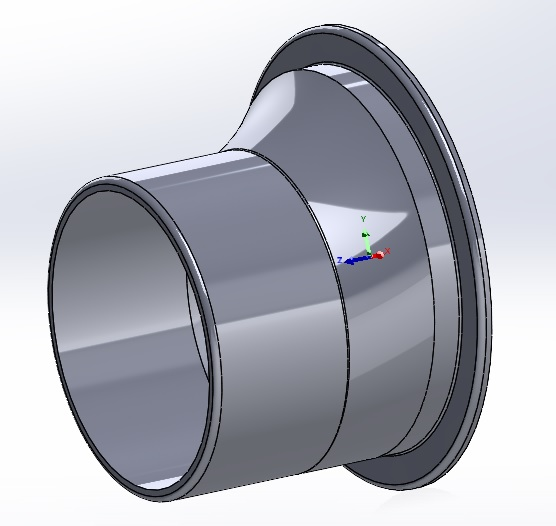
\includegraphics[scale=0.7]{images/Pruebas/Pruebas_S4/cono_excentrico.jpg}
            \caption{Adaptador con cono excéntrico}
            \label{fg:conexcentrico}
 \end{figure}

\clearpage

\subsection{Sistema de procesamiento de materia $S_5$}


\textbf{Trabajo en el contenedor}

Se llevó a cabo un paso crucial enfocado en la preservación y durabilidad del contenedor destinado para la elaboración de este proyecto ya que, aunque se encontraba pintado, fue necesario despintar lo puesto que el recubrimiento que tenía ya presentaba algunos daños debido al traslado y el tiempo que pasó en la intemperie. Por otro lado, una vez despintado se notó que el tambo comenzaba a oxidarse.

Para contrarrestar este proceso corrosivo, se buscó adquirir una pintura que resista las altas temperaturas, esto debido a que el tambo será calentado constantemente.

Previo a pintar el tambo, se procedió a lijar aquellas partes oxidadas, una vez lijado se aplicaron dos capas de pintura, tanto por fuera, como por dentro del contenedor, obteniendo el siguiente resultado:

\begin{figure}[h!]
            \centering
            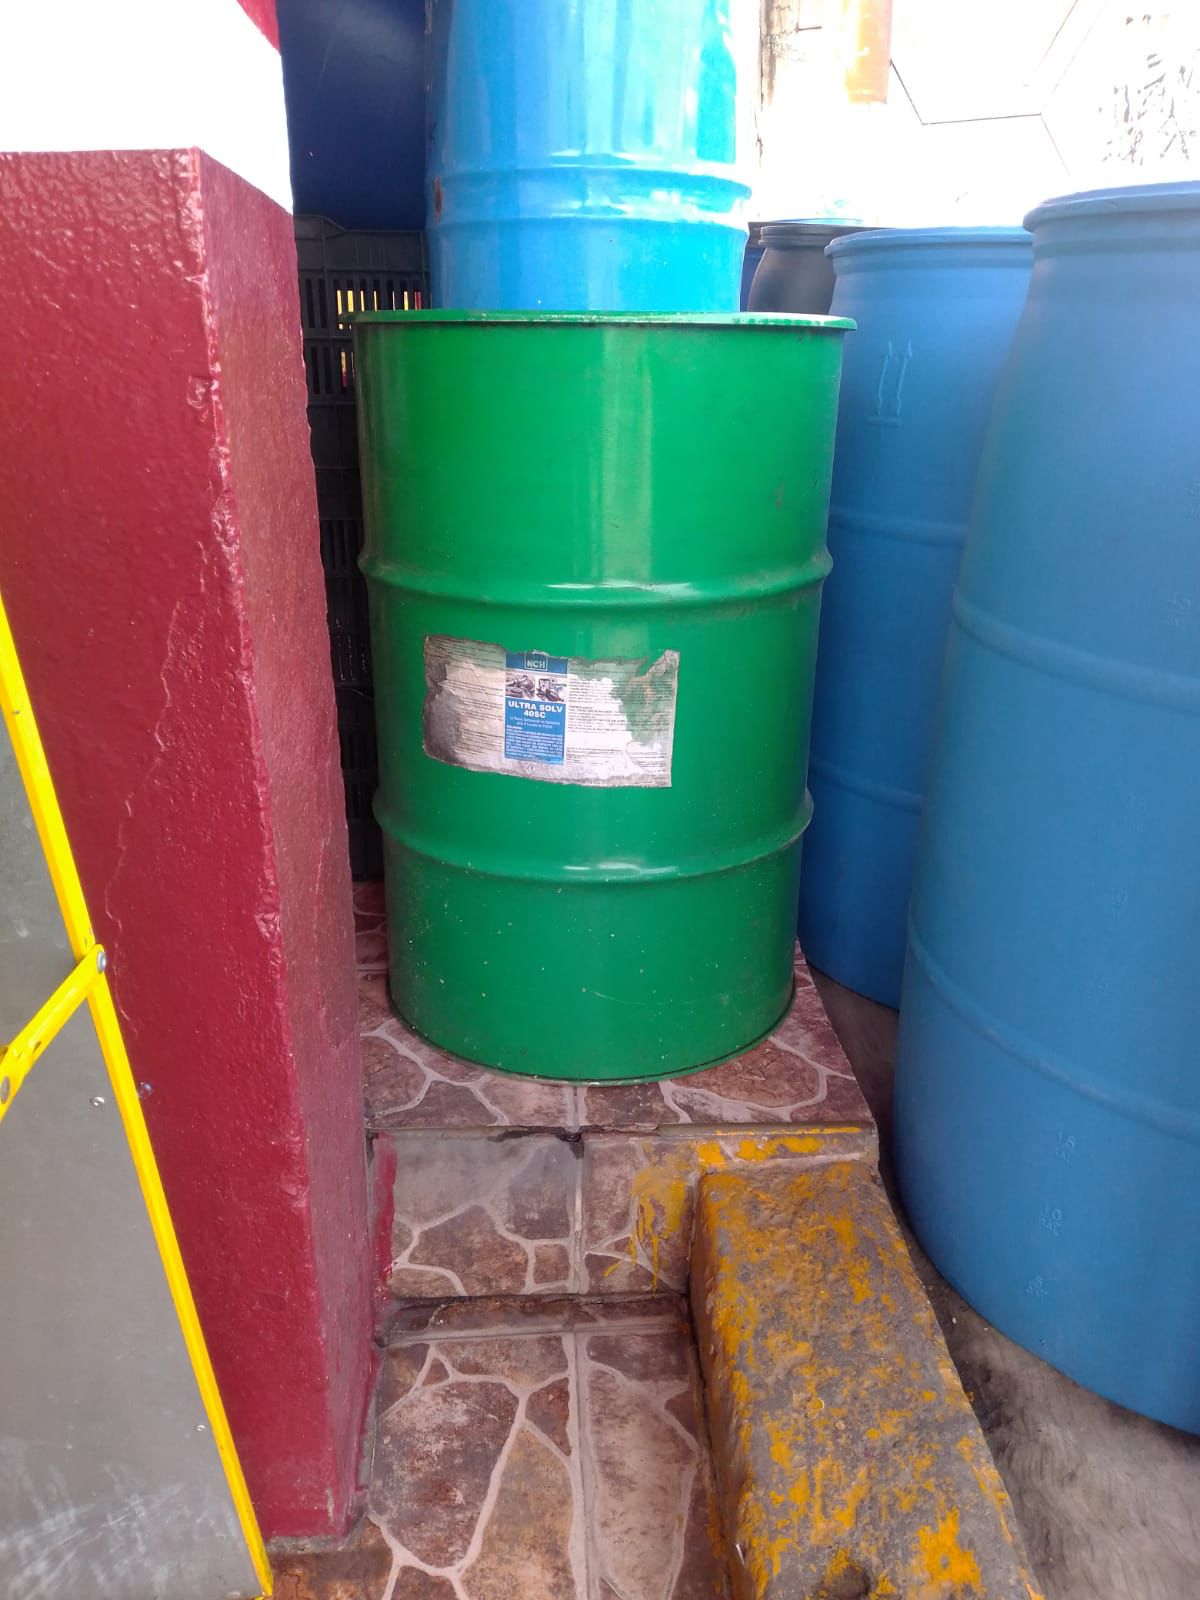
\includegraphics[scale=0.17]{images/Capitulo 4/s5/Contenedor/Contenedor_imple/contenedor_antes.jpg}
            \caption{Contenedor de acero antes}
            \label{fg:tambo_antes}
        \end{figure}
        
\newpage
\begin{figure}[h!]
            \centering
            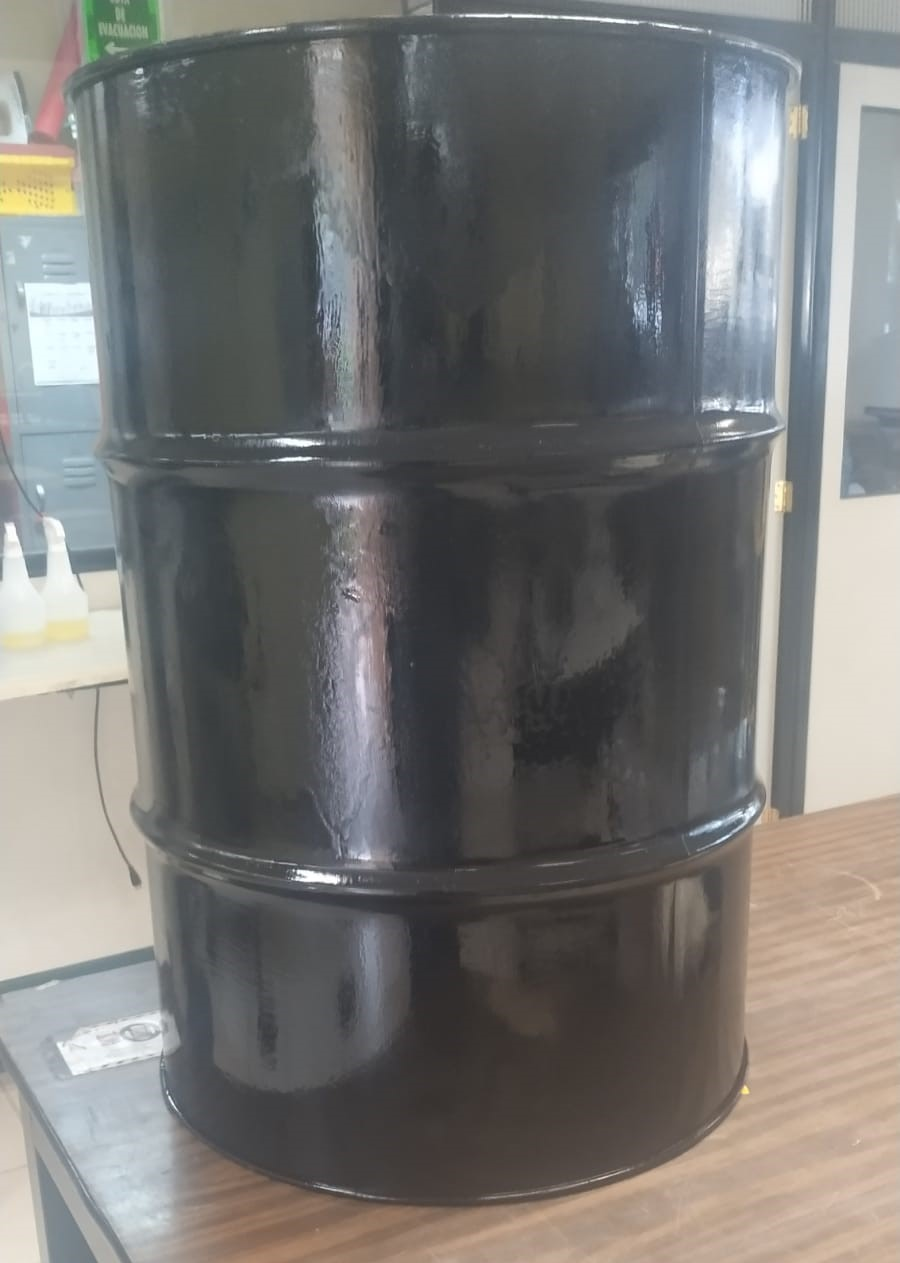
\includegraphics[scale=0.18]{images/Capitulo 4/s5/Contenedor/Contenedor_imple/contenedor_despues.jpg}
            \caption{Contenedor de acero con una capa de pintura}
            \label{fg:tambo_antes}
        \end{figure}

Posteriormente, se colocó el contenedor en la estructura y se marcaron las referencias para el paso del eje. Mediante un sacabocados se procedió a realizar las perforaciones y con ayuda de una lima se rebajó los bordes para que el eje entrara con el mínimo de juego posible.

\begin{figure}[h!]
            \centering
            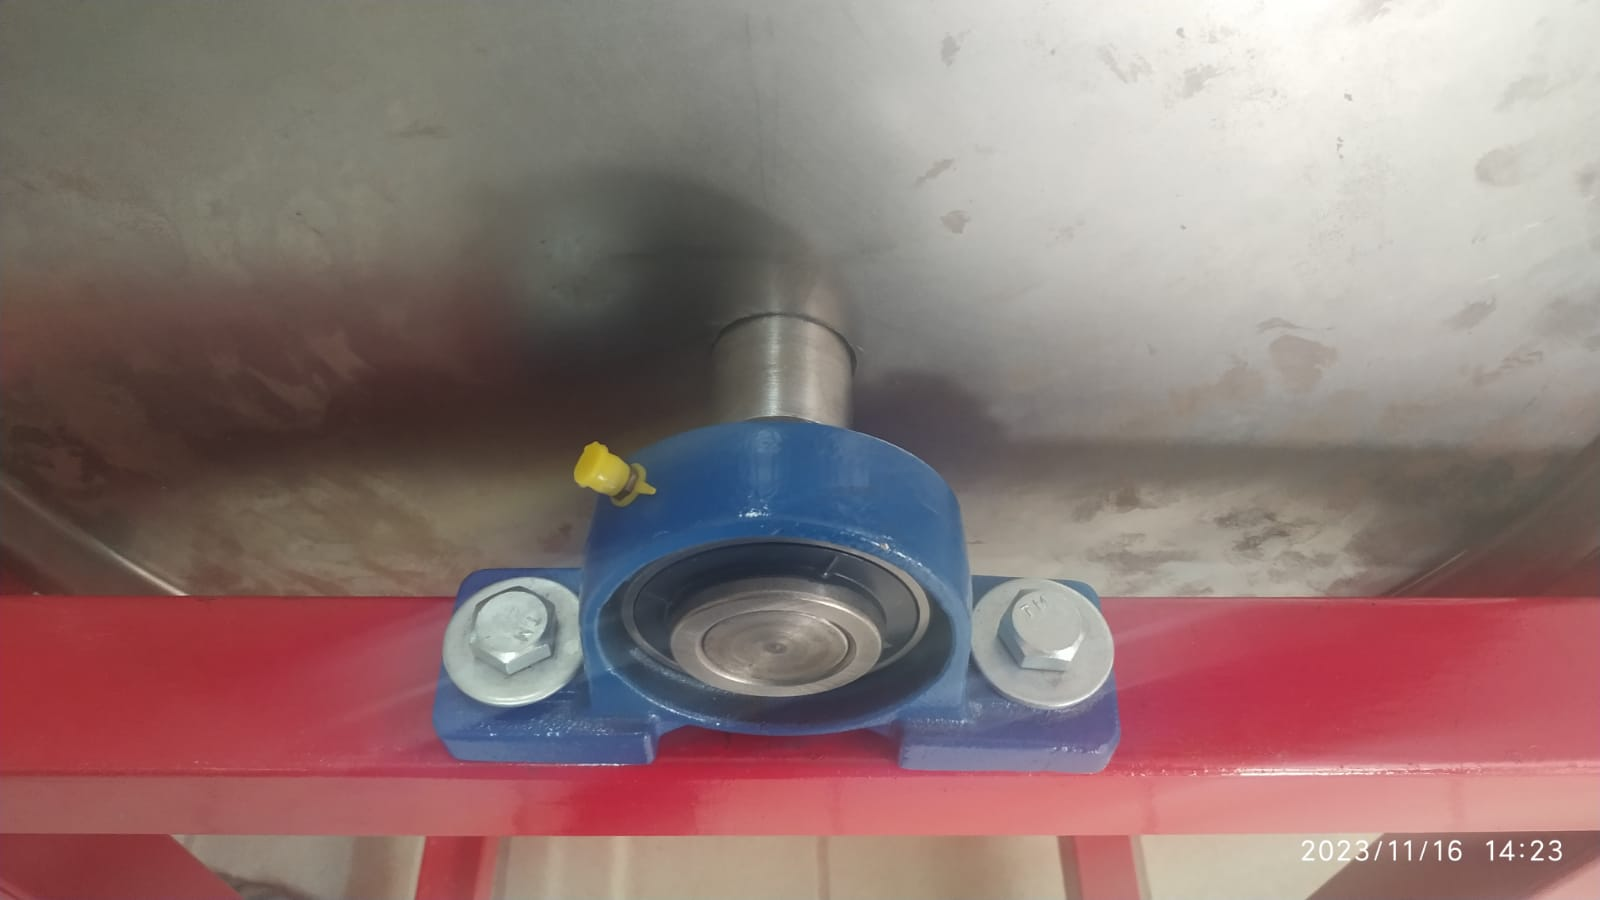
\includegraphics[scale=0.2]{images/Capitulo 4/s5/Contenedor/Contenedor_imple/tambo_montado.jpg}
            \caption{Contenedor montado en el eje}
            \label{fg:tambo_montado}
        \end{figure}
        \newpage
\textbf{Sistema de autorregulación de temperatura
}
Para la implementación de este sistema, se realizó un gran ajuste. Debido a los riesgos que implicaban tener las resistencias eléctricas expuestas, tales como quemaduras y riesgo de un corto circuito, además de su muy baja eficiencia, se optó por revisar otras soluciones disponibles en el mercado. 

De esta manera, se llegó a la conclusión de utilizar un cinturón especial para calentamiento de tambos de aceite, como el de la figura \ref{fg:cinturon_calentador}.  Este dispositivo si es mas caro a comparación de las resistencias, pero nos ofrece mayor seguridad, cubriendo las resistencias 

\begin{figure}[h!]
            \centering
            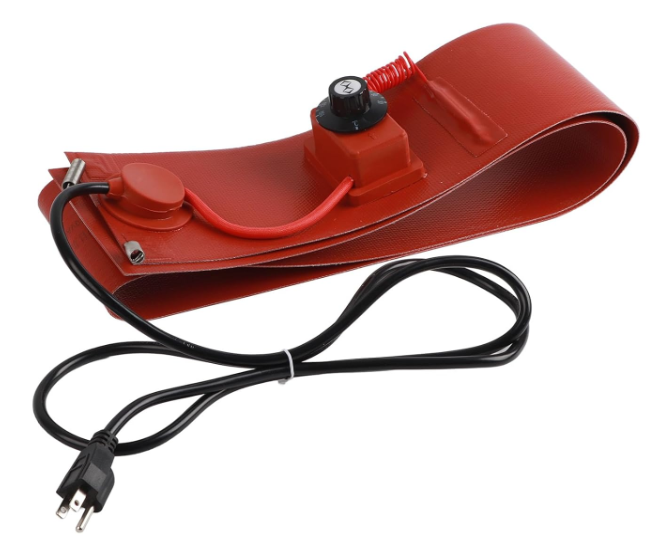
\includegraphics[scale=0.2]{images/Capitulo_Imple/S5/Actuadores/calentador.png}
            \caption{Cinturón calentador de tambos}
            \label{fg:cinturon_calentador}
        \end{figure}
        Este sistema rodea la parte central del tambo, estará directamente configurado para calentar la pared del contenedor a una temperatura de $100 °C$ y estará controlado por medio de un controlador "On/OFF" que sera el encargado de encenderlo únicamente cuando sea necesario.

        En las pruebas que se realizaron, se comprobó que es capas de transmitir el calor al interior a la materia dentro del contenedor, llegando a una temperatura de $75 °C$ en aproximadamente 10 minutos. Además de solo consumir un $1 Kw/hr$ de energía.
        
\textbf{Sistema de ventilación}

Para este sistema fue necesario diseñar una pieza que permita conectar la salida del contenedor, a la entrada del filtro, dada la forma del contenedor resultaba imposible colocarlo directamente.
Se procedió a diseñar la pieza en SolidWorks en donde se obtuvo el siguiente resultado:

\begin{figure}[h]
            \centering
            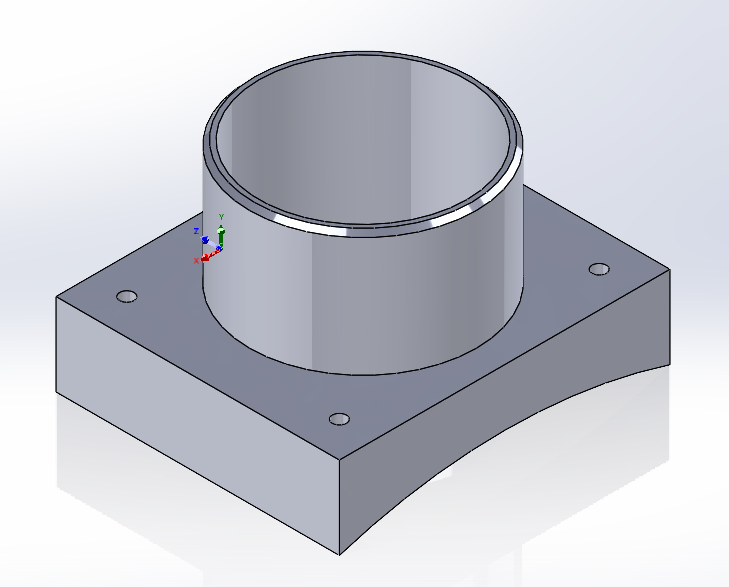
\includegraphics[scale=0.35]{images/Capitulo 4/s5/Contenedor/Contenedor_imple/adaptador_filtro.png}
            \caption{Adaptador para filtro}
            \label{fg:adap_filtro}
 \end{figure}

Dado que la pieza presenta una geometría bastante particular, la mejor opción fue imprimirla en 3D. Se procedió a ajustar algunos detalles previo a la impresión, teniendo un estimado de 13 horas para le impresión total de la pieza.

\begin{figure}[h]
            \centering
            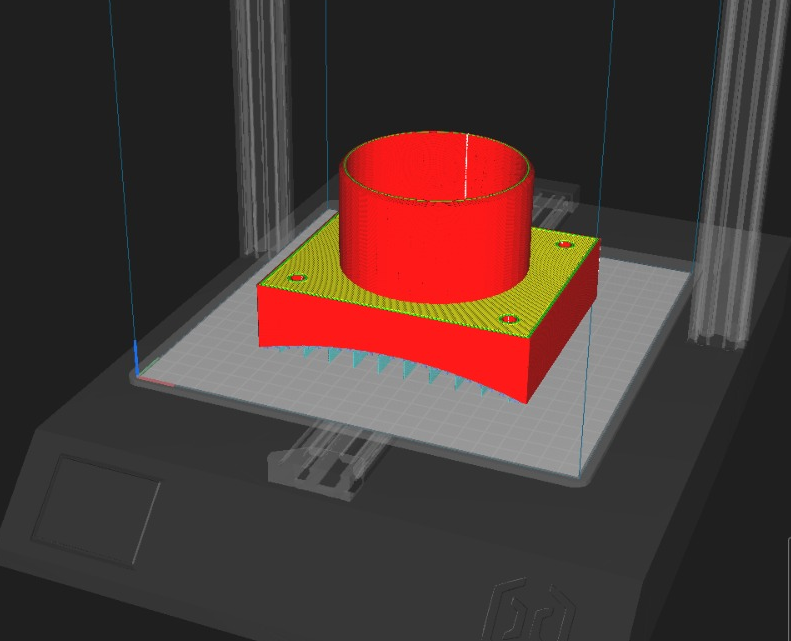
\includegraphics[scale=0.32]{images/Capitulo 4/s5/Contenedor/Contenedor_imple/imp_filtro_1.png}
            \caption{Ajuste de parámetros software de impresión}
            \label{fg:impresion_filtro1}
 \end{figure}
 \newpage
Posteriormente se realizó el proceso de impresión obteniendo:
\begin{figure}[h]
            \centering
            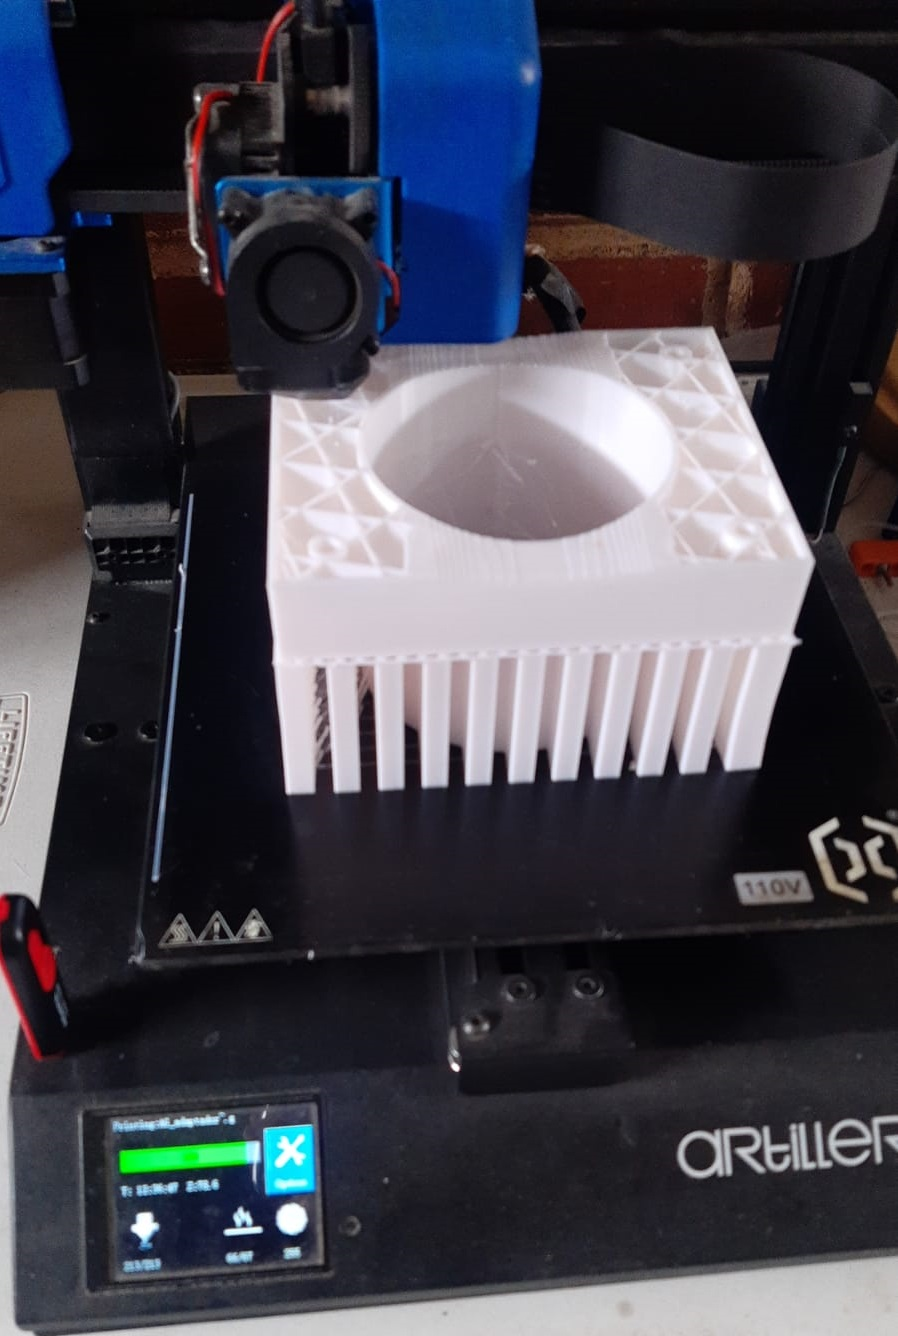
\includegraphics[scale=0.18]{images/Capitulo 4/s5/Contenedor/Contenedor_imple/imp_filtro_2.jpg}
            \caption{Impresión 3D adaptador para filtro}
            \label{fg:impresion_filtro2}
 \end{figure}

 Una vez impresa la pieza, se retiraron los soportes que coloca la impresora para que la pieza no pierda su forma y se procedió a colocar la pieza en el contenedor, se realizaron algunos barrenos en el tambo para poder fijarla.

 \begin{figure}[h]
            \centering
            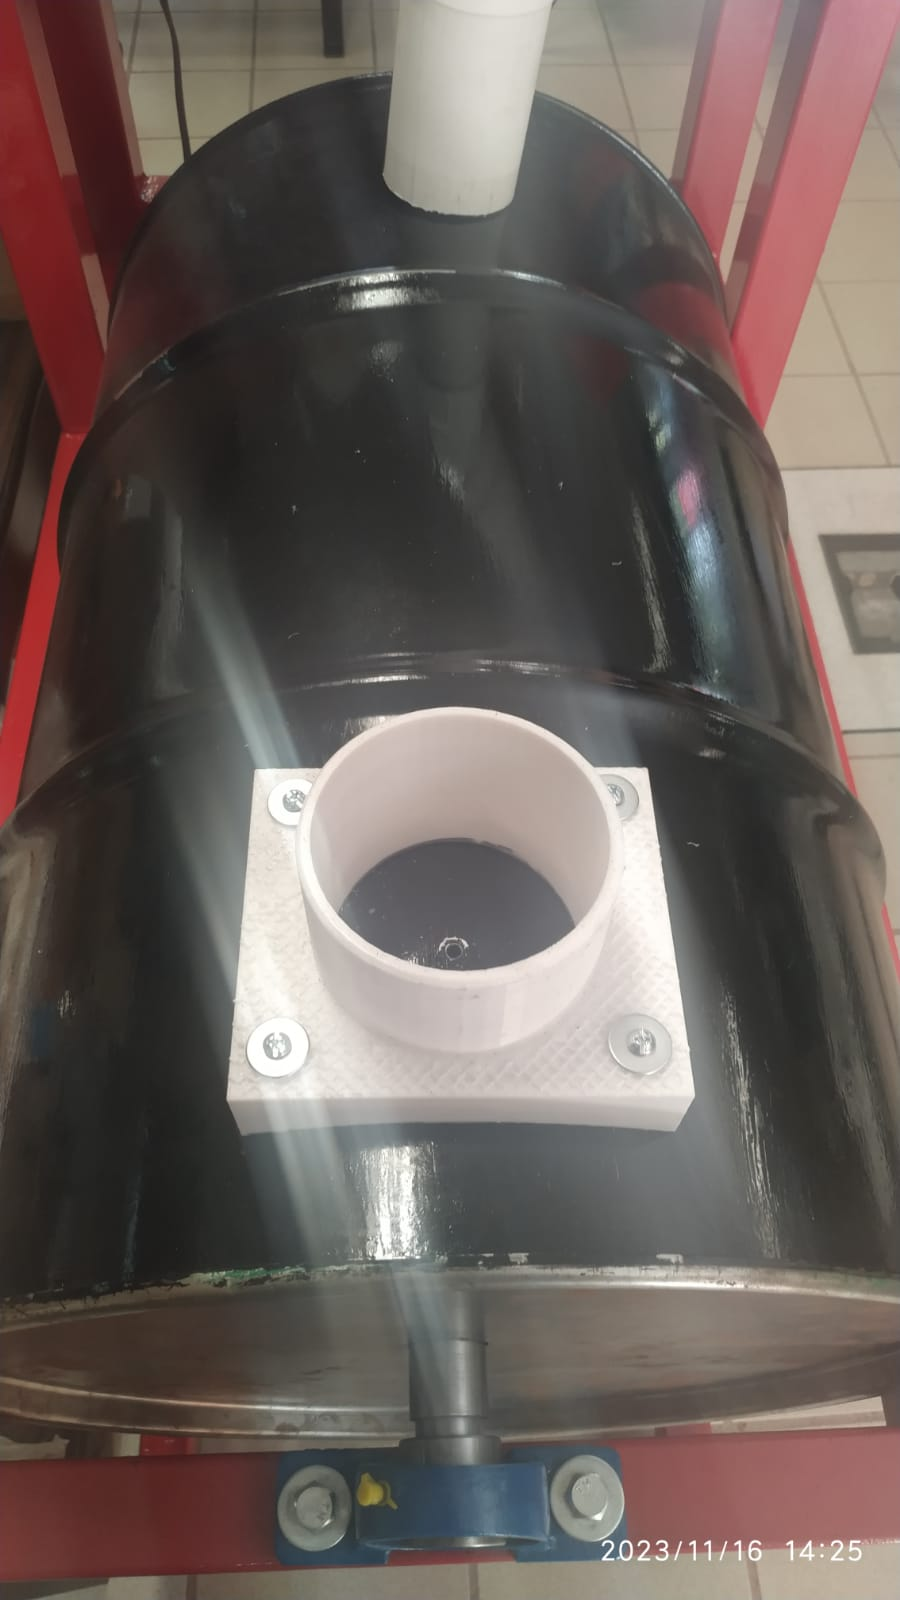
\includegraphics[scale=0.1]{images/Capitulo 4/s5/Contenedor/Contenedor_imple/adaptadorfilt_montado2.jpg}
            \caption{Adaptador montado en el contenedor}
            \label{fg:adaptador_montado_tambo}
 \end{figure}

 \newpage
 \begin{figure}[h]
            \centering
            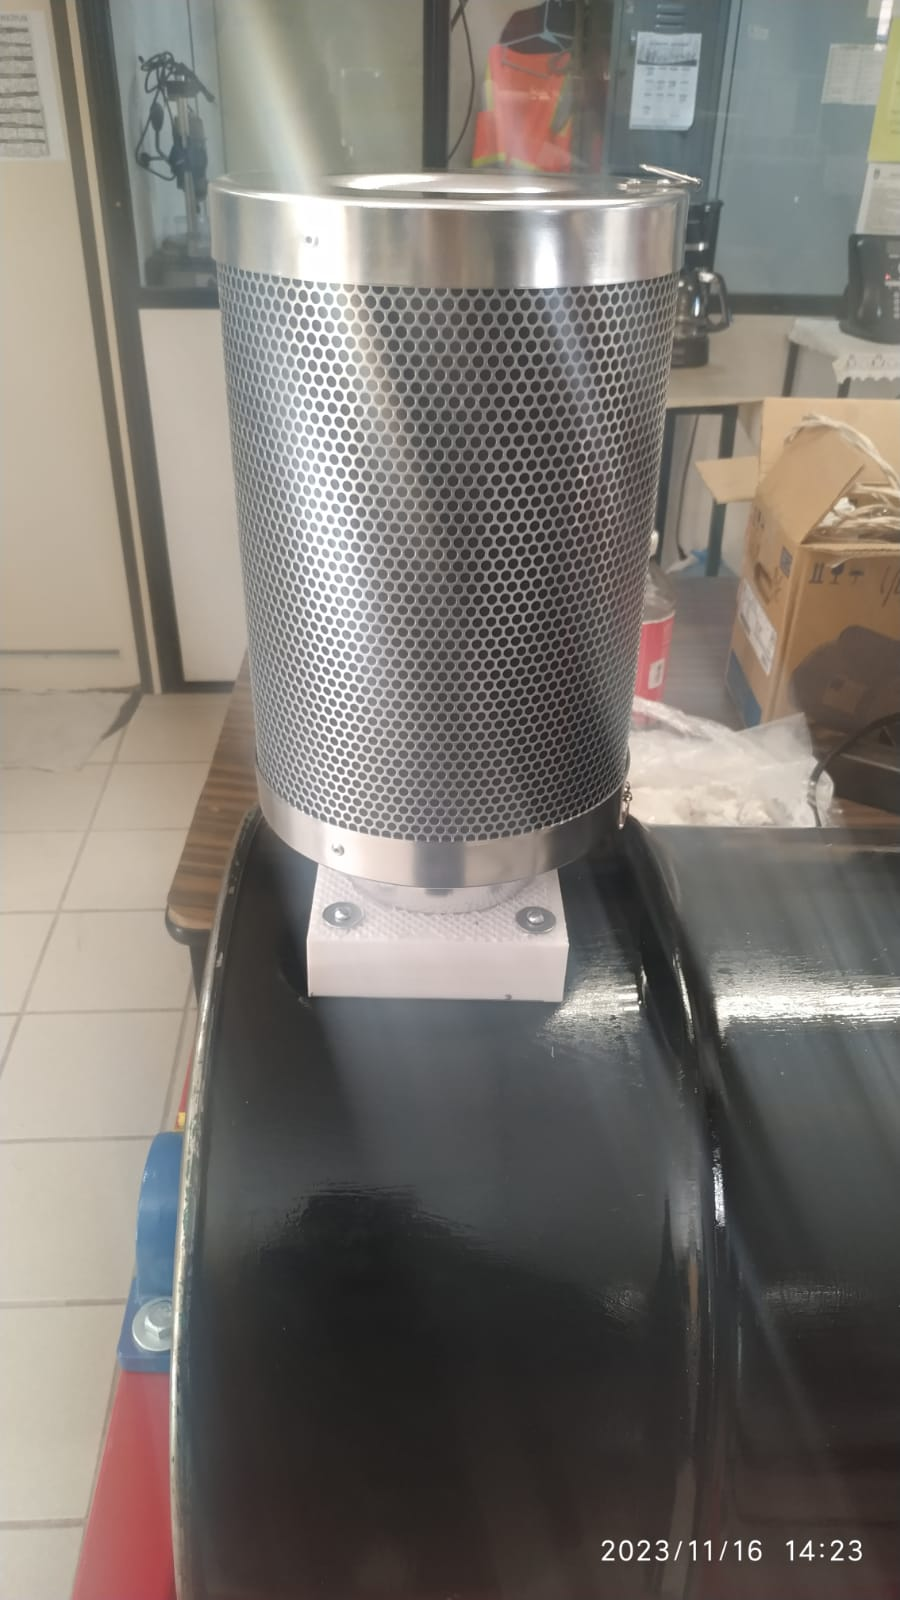
\includegraphics[scale=0.15]{images/Capitulo 4/s5/Contenedor/Contenedor_imple/adaptadorfilt_montado.jpg}
            \caption{Adaptador ensamblado con filtro}
            \label{fg:adaptador_filtro_montados}
 \end{figure}
Para facilitar la entrada de aire al contenedor, se empleó un ventilador de computadora de 3'', por lo que fue necesario diseñar una pieza que permitiera enlazarlo a la estructura de PVC, en consecuencia se modeló una base para el ventilador en SolidWorks, esta pieza fue impresa en 3D obteniéndose el siguiente resultado:
 \begin{figure}[h]
            \centering
            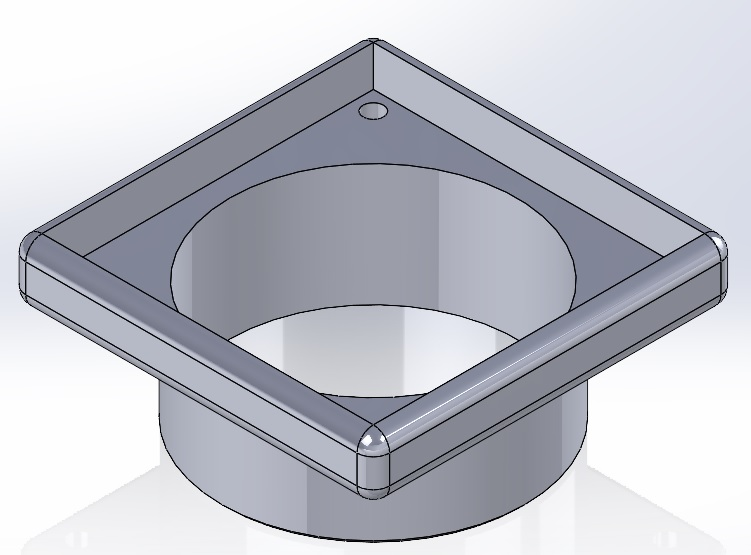
\includegraphics[scale=0.15]{images/Pruebas_S5/pieza_ventilador.jpg}
            \caption{Diseño adaptador para ventilador en SolidWorks}
            \label{fg:adaptador_ventilador}
            
 \end{figure}
  \begin{figure}[h]
            \centering
            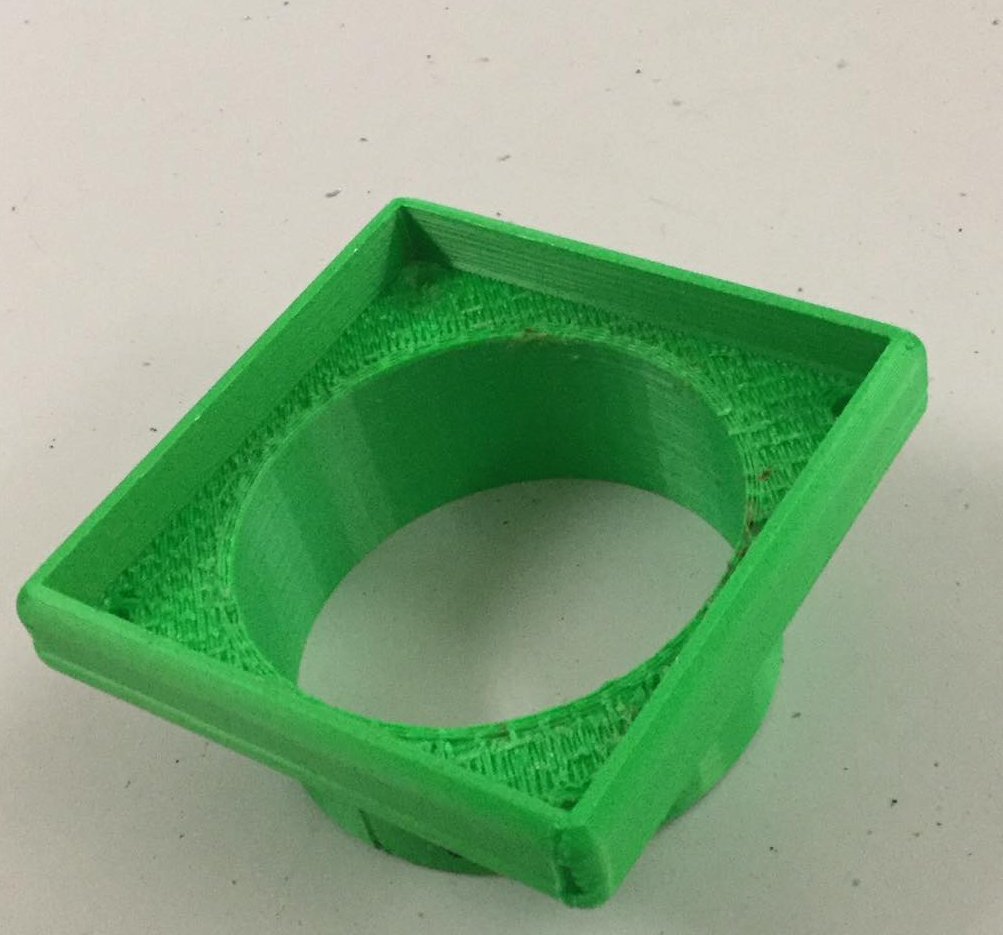
\includegraphics[scale=0.15]{images/Pruebas_S5/pieza_ventilador_impresa.png}
            \caption{Impresión 3D adaptador para ventilador}
            \label{fg:adaptador_ventilador}
            
 \end{figure}
\textbf{ Sistema de aireación}

 Para el sistema de aireación, se realizó la manufactura del eje a partir de un tajo de acero, el cual se manipuló a través de un torno, aplicando las operaciones de careado, cilindrado y desbaste para generar cada una de las secciones funcionales del eje.

 Este elemento tiene un diámetro de $1 \frac{1}{2} in$ por lo que fue necesario conseguir las chumaceras de esta medida para sostener el eje el la estructura y a su vez permitirle girar sin riesgo de fricción.

 En uno de los extremos del eje, se coloco una polea, la cual esta fijada con un esclavo, un anillo de acero y una chaveta para transmitir el movimiento proveniente de un motor de corriente alterna de $\frac{1}{4} Hp$. 

 El motor esta conectado a una reductor de $\frac{1}{40}$ y tiene una polea de salida $2 \frac{1}{2} in$
 por lo que se al final, el eje estará girando a una velocidad de 6 $rpm$, velocidad suficiente para realizar el proceso de aireación y mezcla de los desechos a su interior (Figura \ref{fg:montaje airo}.

 También ofrece el momento necesario para poder voltear los 20 $kg$ de materia que se pretenden procesar en su interior.

 Este motor eléctrico es activado por medio de una señal que sale de la ESP32, el cual abre la señal para la activación de un contactor eléctrico, el cual es capaz de soportar la corriente de arranque del motor eléctrico y de esta forma, se puede llevar a cabo el proceso de aireación de forma automática.

  \begin{figure}[h]
            \centering
            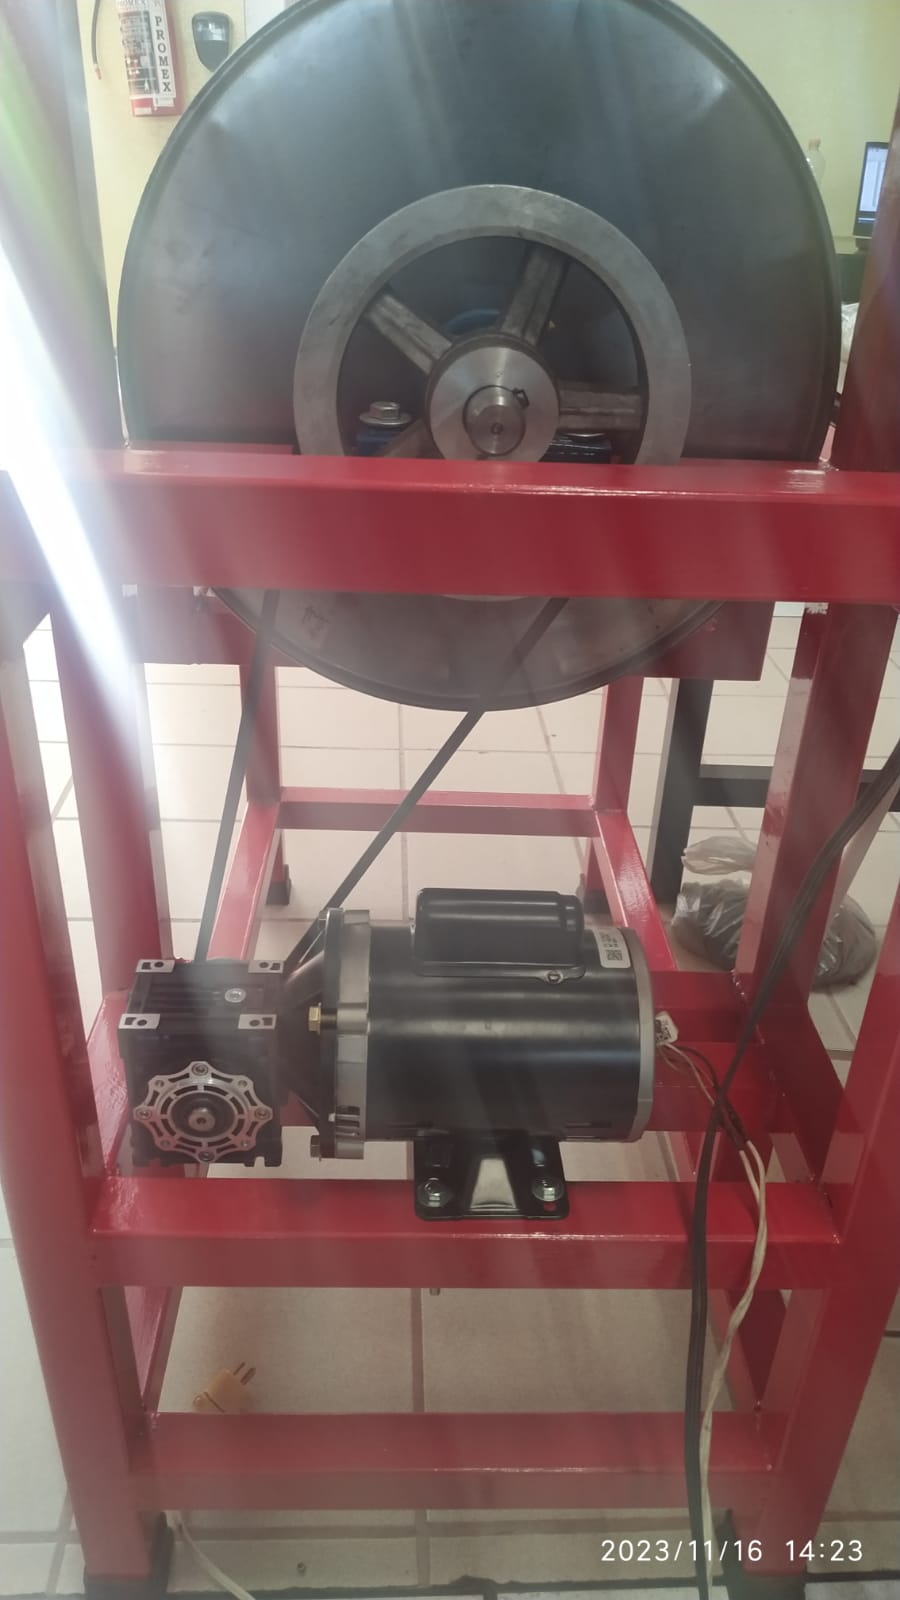
\includegraphics[scale=0.2]{images/Capitulo_Imple/S5/Aireacion.jpeg}
            \caption{Montaje del sistema de aireación}
            \label{fg:montaje airo}
 \end{figure}
 Para la construcción del sistema de palas, se utilizaron secciones de tubo con cuerda, a las que por medio de un esmeril se les retiró parte de la cuerda dejándolos como tubos lisos. 
 Posteriormente  se cortaron rectángulos de (medidas ***) de un pedazo de tubo rectangular para la fabricación de las palas, se optó por esa disposición de palas debido a que era necesario revolver de manera uniforme toda la mezcla, y que la formación de surcos podría afectar a la mezcla. 
 El tamaño y disposición de las palas, garantiza que no queden surcos y que toda la materia se mezcle de manera uniforme, lo que en consecuencia permite que el calor se distribuya de manera uniforme en toda la mezcla al igual que al momento de oxigenar.

 Una vez cortadas las palas, se procedió a soldarlas a las secciones de tubo con cuerda, obteniendo el siguiente resultado:

   \begin{figure}[h]
            \centering
            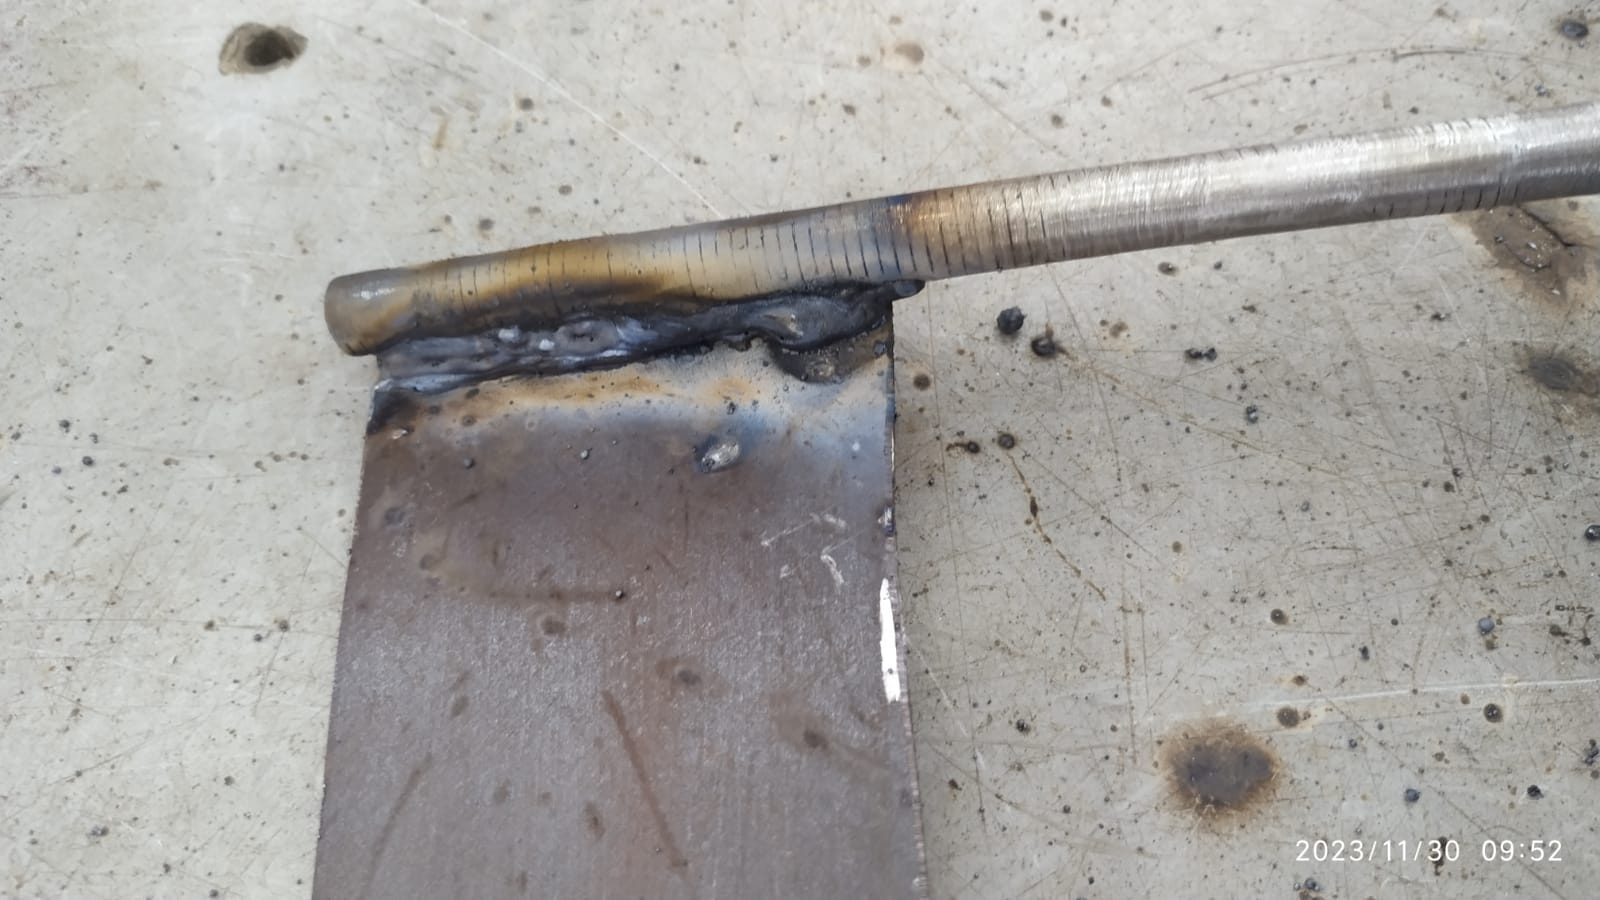
\includegraphics[scale=0.2]{images/Pruebas_S5/pala_soldada.jpeg}
            \caption{Pala soldada a sección de tubo con cuerda}
            \label{fg:soldar_pala}
 \end{figure}


Por último fue necesario realizar un aplanamiento de secciones en el eje  empleando una fresadora. Esto con el fin de facilitar la sujeción de las palas al eje. (Figura \ref{fg:eje_fresado})  

\begin{figure}[h!]
            \centering
            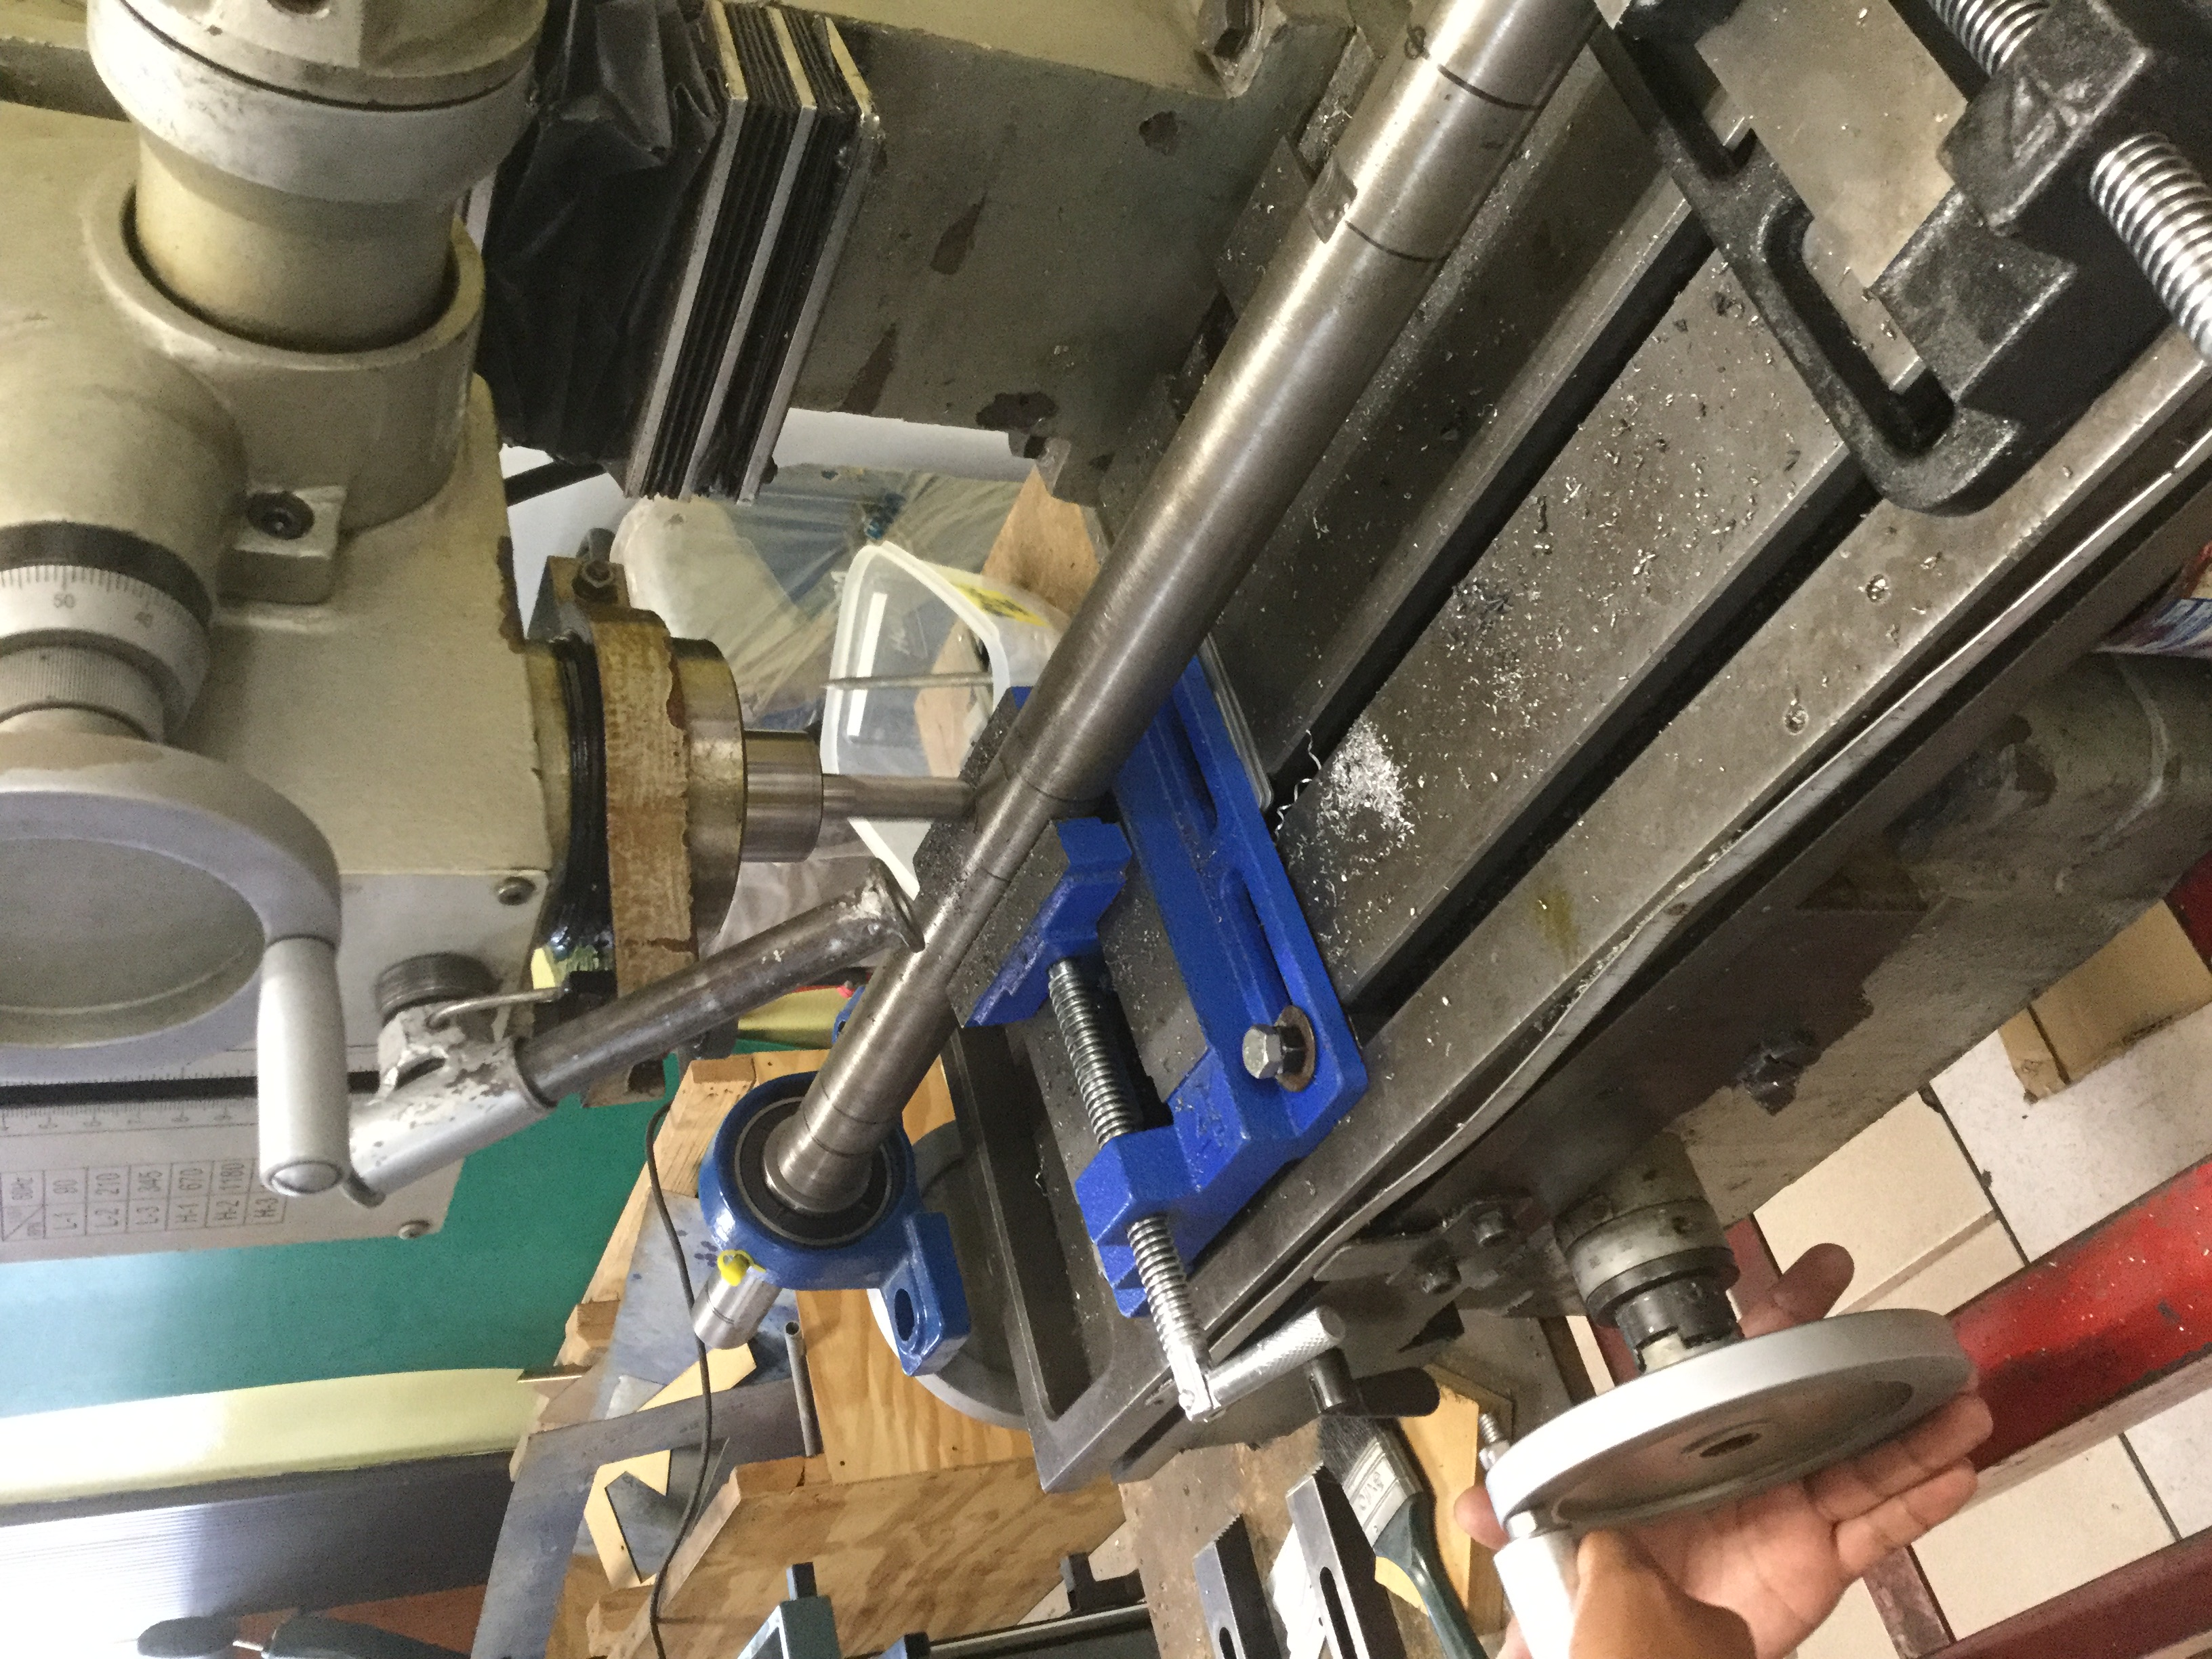
\includegraphics[scale=0.09, angle=270]{images/Capitulo_Imple/S5/fresado.JPG}
            \caption{Proceso de fresado del eje}
            \label{fg:eje_fresado}
        \end{figure}

\textbf{Aislamiento térmico}
Por medio de fibra de vidrio se forró todo el contenedor,  realizando los cortes pertinentes para la salida al filtro, al sistema de triturado y  el cable del cinturón. Para esta parte se colocaron los diversos componentes en su lugar para tomar medidas y realizar los cortes. (Figura \ref{fg:tambo_sin_cubir})

\begin{figure}[h!]
            \centering
            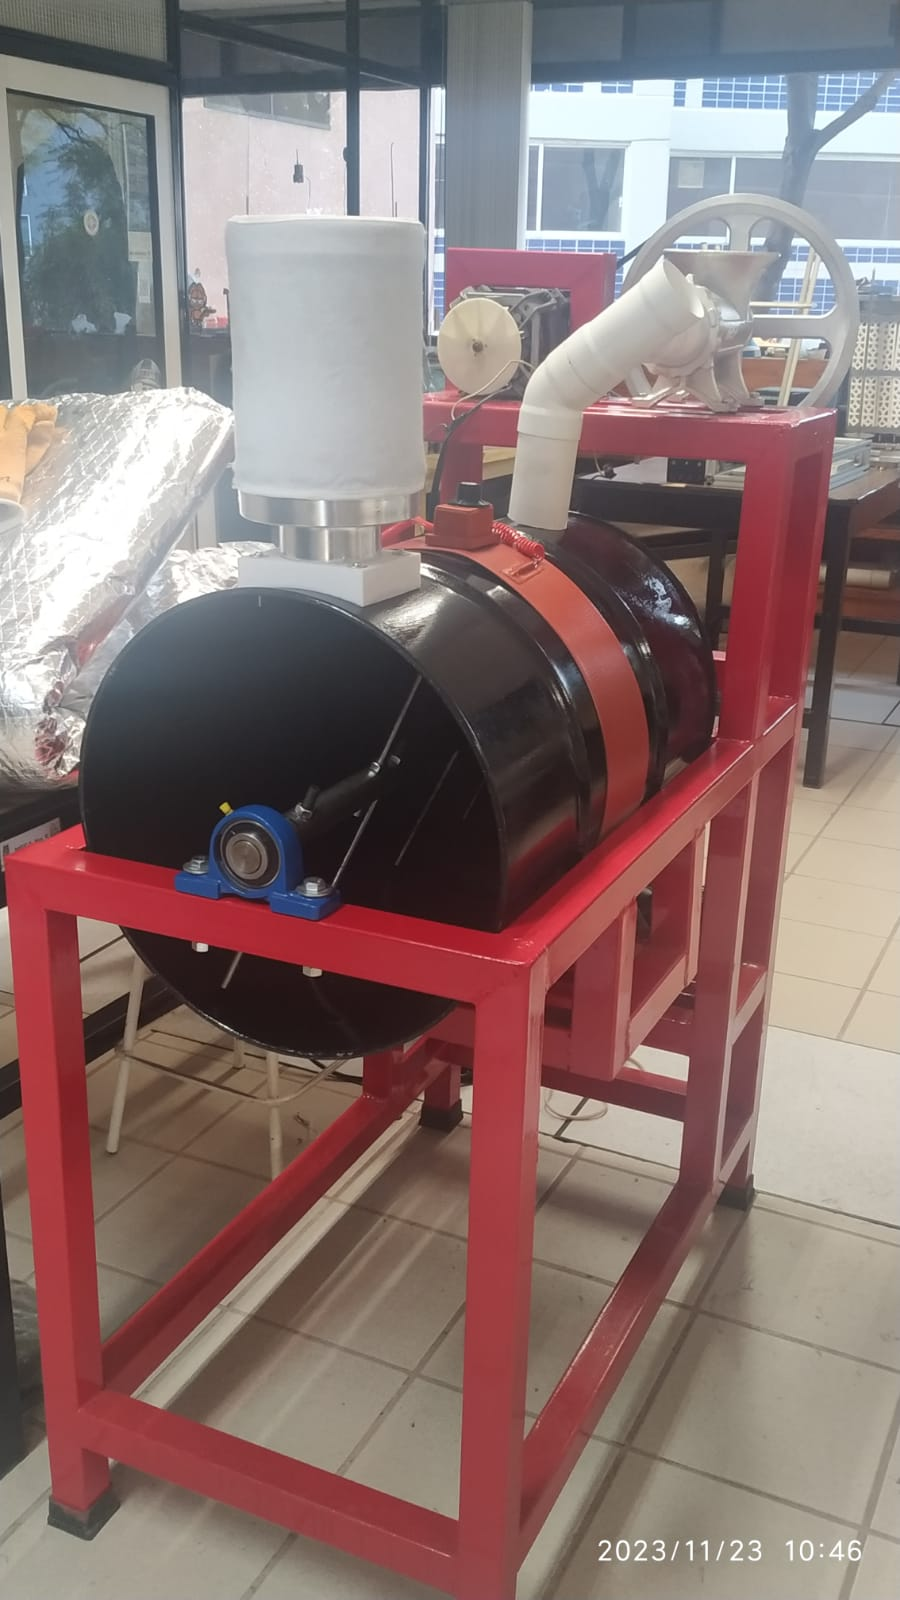
\includegraphics[scale=0.15]{images/Capitulo_Imple/S5/tambo_sin_cubrir.jpeg}
            \caption{Instalación de los elementos del tambo sin recubrimiento}
            \label{fg:tambo_sin_cubir}
        \end{figure}

Para sujetar la fibra, se utilizó una cinta perforada de aluminio, la cual se sujetó con un tornillo y una tuerca. (Figura \ref{fg:tambo_cubierto}).

\begin{figure}[h!]
            \centering
            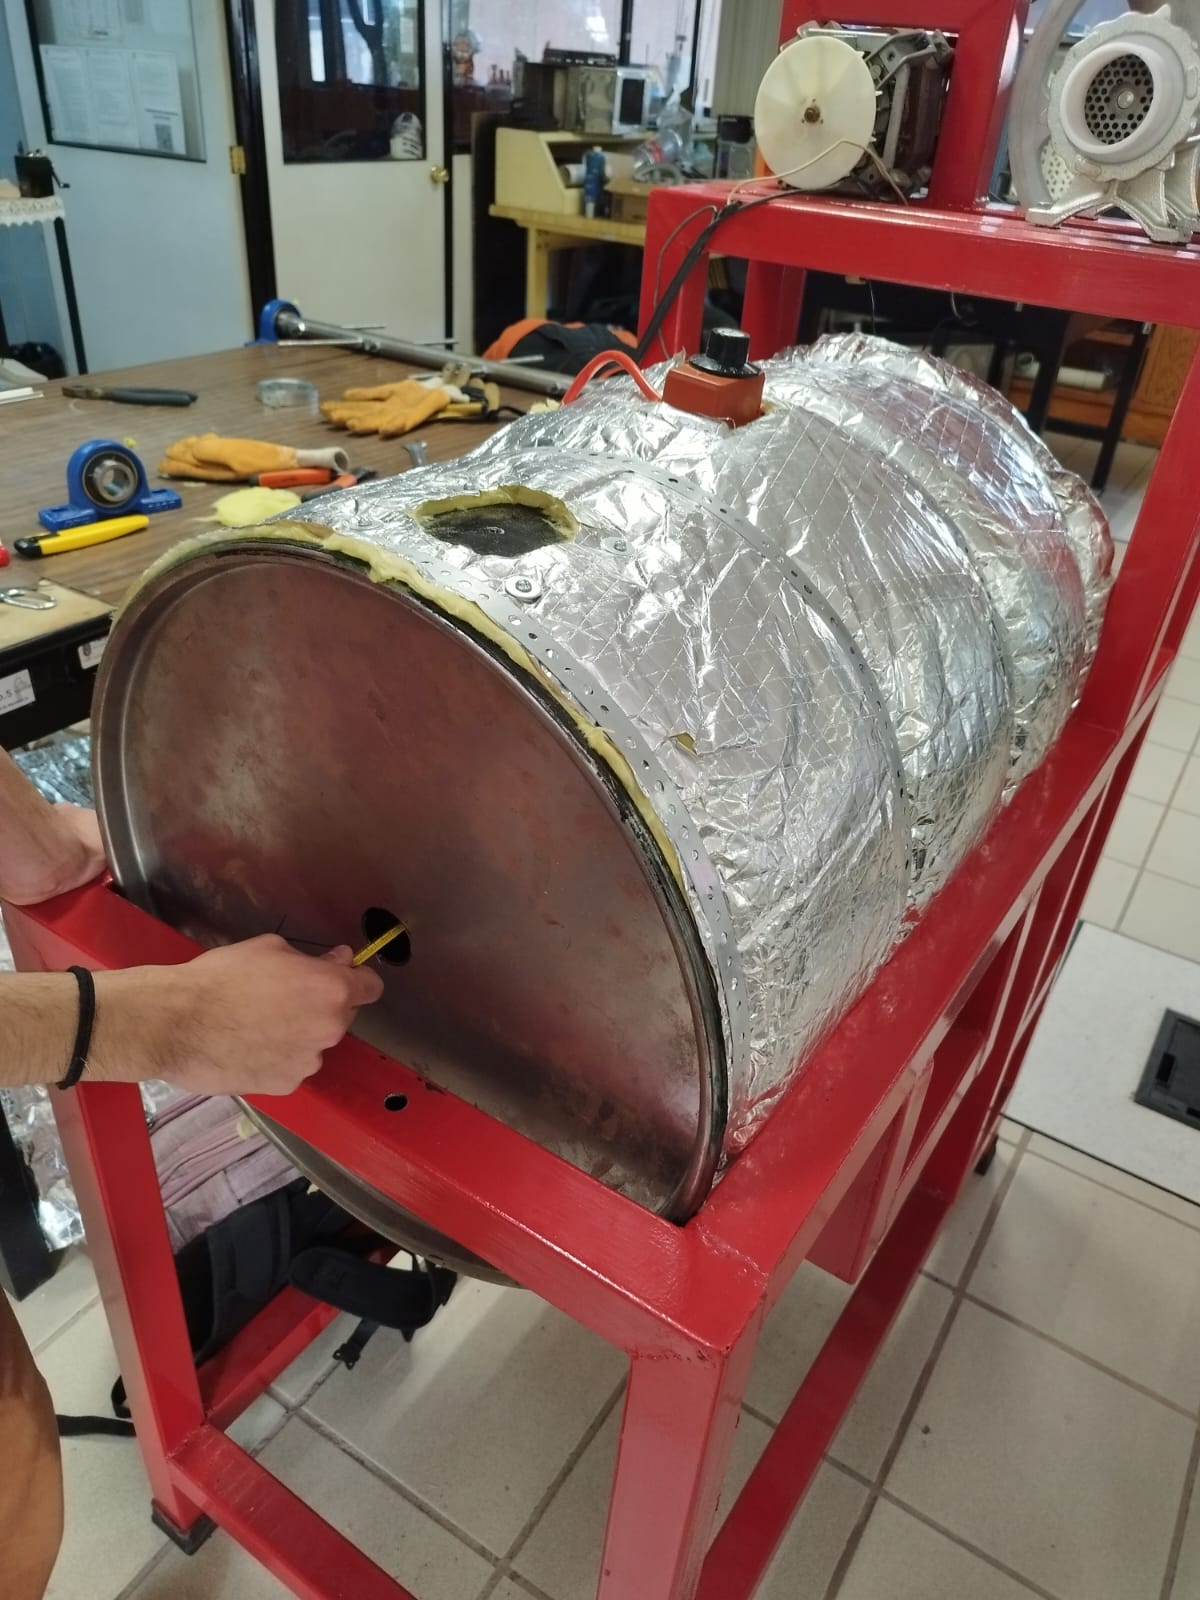
\includegraphics[scale=0.18]{images/Capitulo_Imple/S5/tambo_solo.jpeg}
            \caption{Contenedor con el recubrimiento instalado}
            \label{fg:tambo_cubierto}
        \end{figure}

\textbf{Verificación subsistema 5}
\textbf{Sistema de autorregulación de temperatura
}
Para este sistema se realizaron algunas pruebas, en un primer momento solo se conectó el cinturón para comprobar que este se calentara y observar el comportamiento que presentaba.
Con este sencillo experimento se pudo notar que al calentar, el dispositivo pasa de un color rojo a un color marrón. Posteriormente, se realizaron algunos ensayos colocando tierra en al interior del tambo simulando los desechos vegetales, se procedió a envolver el contenedor con el cinturón y se prosiguió a conectar el cinturón.
Con ayuda de un termómetro se realizaron algunas mediciones de la tierra, previo a encender el cinturón y después de mantenerlo encendido un periodo determinado de tiempo. Al iniciar la prueba la tierra tenía una temperatura de 23°C y después de mantener encendido el dispositivo por un rato se registró una temperatura de 42°C. 

\textbf{Sistema de ventilación}
Durante la fase pruebas del compostador se observaron dos situaciones principalmente , la primera en relación a la salida del vapor generado pro el calentamiento de los desechos, ya que en efecto hay salida de vapor en el filtro puesto que al retirarse dicho componente se puede apreciar cierta condensación del vapor. 
Por otro lado también existe salida de vapor a la entrada del sistema de ventilación, y aunque suene algo contradictorio, esto es algo esperado puesto que cuando el ventilador se encuentra apagado esta zona presenta una menor resistencia al paso del vapor, por solo que este sale sin problema alguno.

Asimismo cuando el ventilador se enciende, se observó una rápida disminución de la temperatura al interior del contenedor, un comportamiento deseable pues permite enfriar el interior de ser necesario y al mismo tiempo introduce oxígeno a la mezcla, es por ello que se propuso incorporarlo al sistema, cabe señalar que en los días fríos pueda disminuir su uso pues es cuando mayores pérdidas de calor se tengan caso contrario a los días calurosos de verano.

\newpage
\subsection{Sistema estructural $S_6$}

\textbf{Elaboración de la estructura}

El material que se utilizo para fabricación de la estructura, fue un perfil cuadrado de 4 $in$, por lo que fue necesario realizar cortes con ayuda de una sierra de banco, utilizar herramientas para cuadrad las piezas y por ultimo soldar cada una de las uniones utilizando el método de soldadura con electrodo.

Una vez que se terminaron de soldar todas las partes, fue necesario realizar un proceso de rectificado en cada una de las uniones con el fin de retirar las imperfecciones de la soldadura y darle una mejor presentación al trabajo.

Con el mismo propósito, se pinto la estructura utilizando un esmalte anticorrosivo, donde se eligió el color rojo por citerior de estética.

Por ultimo, se fueron realizando todas las perforaciones necesarias para atornillar y fijar cada uno de os elementos del sistema de compostaje. El resultado se puede apreciar en la figura \ref{fg:estructura elaborada}.

 \begin{figure}[h]
            \centering
            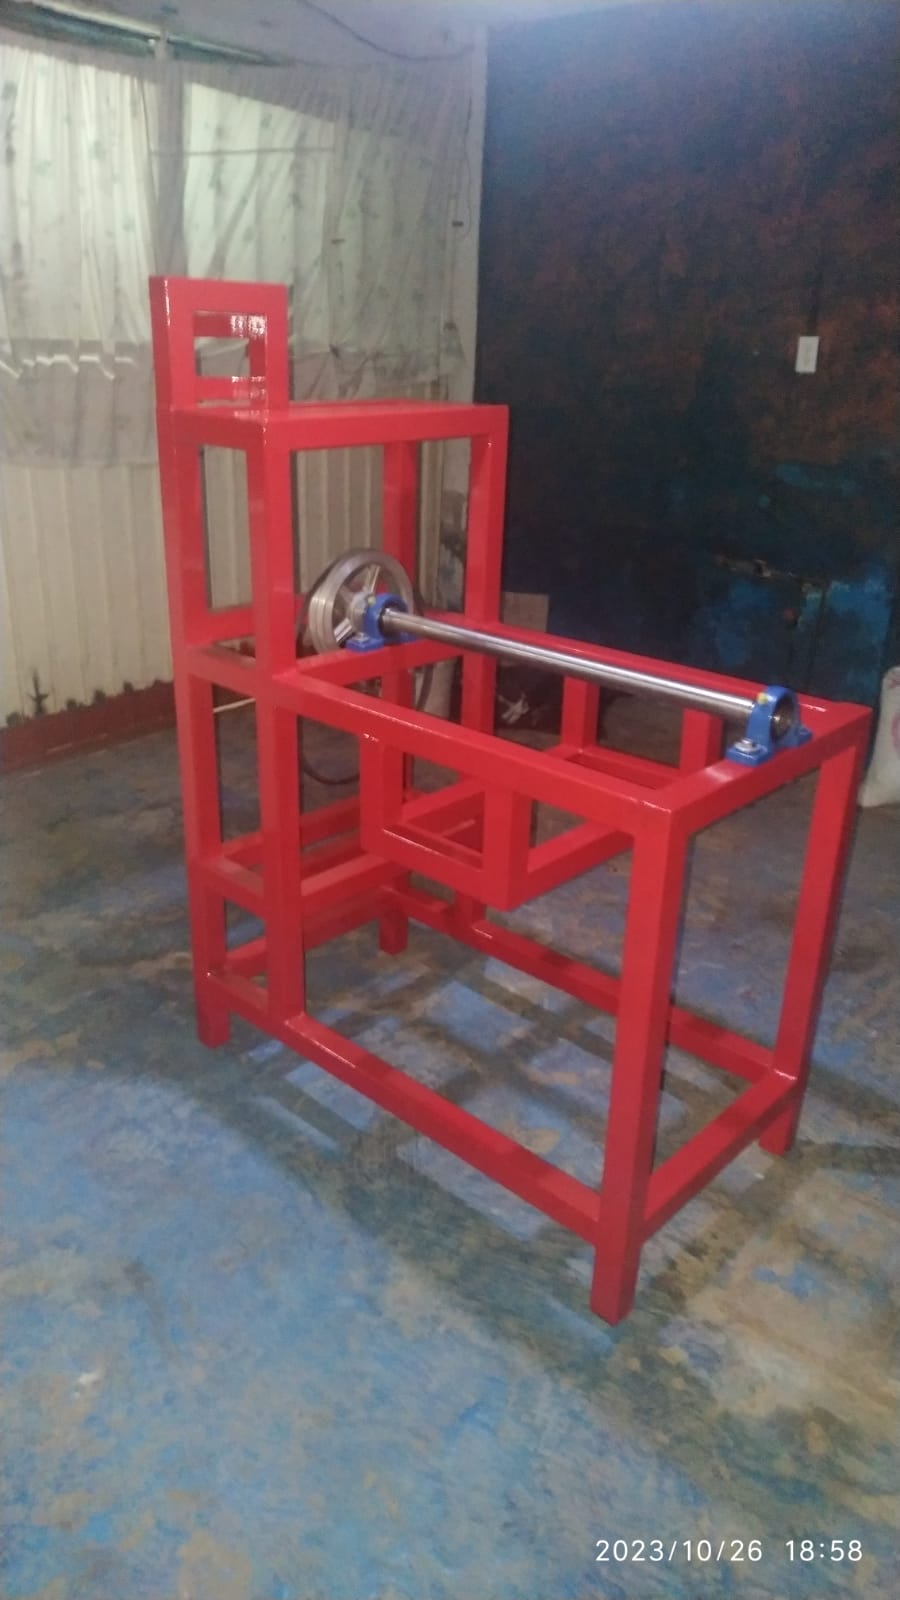
\includegraphics[scale=0.135]{images/Capitulo_Imple/S6/estructura.jpeg}
            \caption{Estructura del sistema de compostaje}
            \label{fg:estructura elaborada}
 \end{figure}

 \clearpage



\textbf{Verificación subsistema 6}
Para verificar la estructura fue necesario montar los diferentes componentes mecánicos que integran el proyecto, de tal forma que no solo se verificó la rigidez y estabilidad de la estructura, sino también que los distintos componentes pudieran situarse de manera adecuada a la estructura.

 \begin{figure}[h]
            \centering
            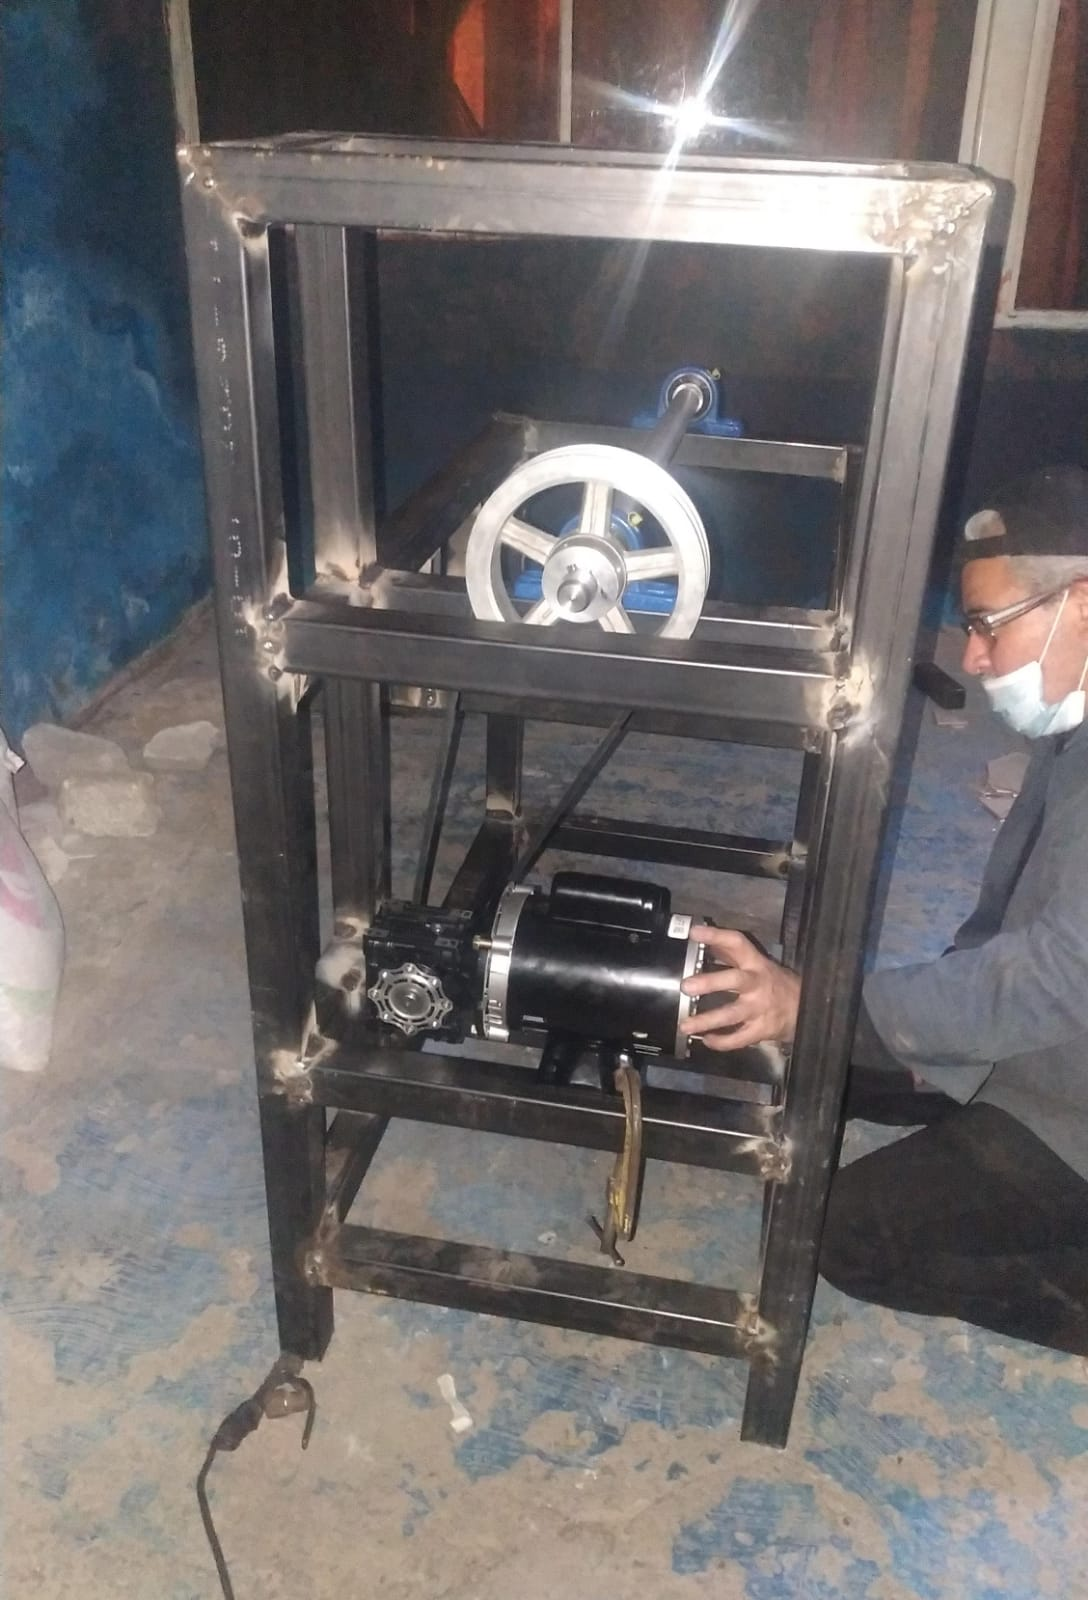
\includegraphics[scale=0.135]{images/Pruebas_S6/montar_componentes.jpeg}
            \caption{Montaje de componentes en estructura}
            \label{fg:estructura elaborada}
 \end{figure}

A diferencia del modelo 3D que se tenía en un inicio para la estructura, fue necesario agregar soportes que permitieran colocar el motor para el sistema de trituración, teniendo como resultado una estructura apta para integrar todos los componentes y mecanismos necesarios para el correcto funcionamiento del sistema.

Durante la realización de la estructura resaltó la necesidad de disminuir el espacio donde se colocaría el contenedor, ya que existía un espacio de aproximadamente media pulgada entre las paredes laterales del contenedor y los lados de la estructura, también se redujo a lo largo una pulgada, para que el contenedor no pudiera desplazarse de atrás hacia adelante.

Finalmente fue necesario colocar soportes que permitieran fijar el triturador y el motor de aireación, ya que en un inicio se consideró colocar una placa de acero, sin embargo se opto por soldar PTR debido a que resultaba más fácil y barato que adquirir una placa de acero con el suficiente espesor para evitar deformaciones.
\newpage
\subsection{Integración del sistema}

Una vez elaborado y probado cada uno de los subsistemas, se fueron integrando respetando la relación existente entre cada uno de los módulos elaborados.

La primera parte fue la integración entre los elementos del sistema de procesamiento de la materia, instalando el eje de aireación dentro del contenedor que a su vez, es instalado sobre la estructura principal. Se realizaron pruebas para verificar que el sistema fuera capaz de operar sin algún problema. (Figura \ref{fg:palas_dentro})

 \begin{figure}[h!]
            \centering
            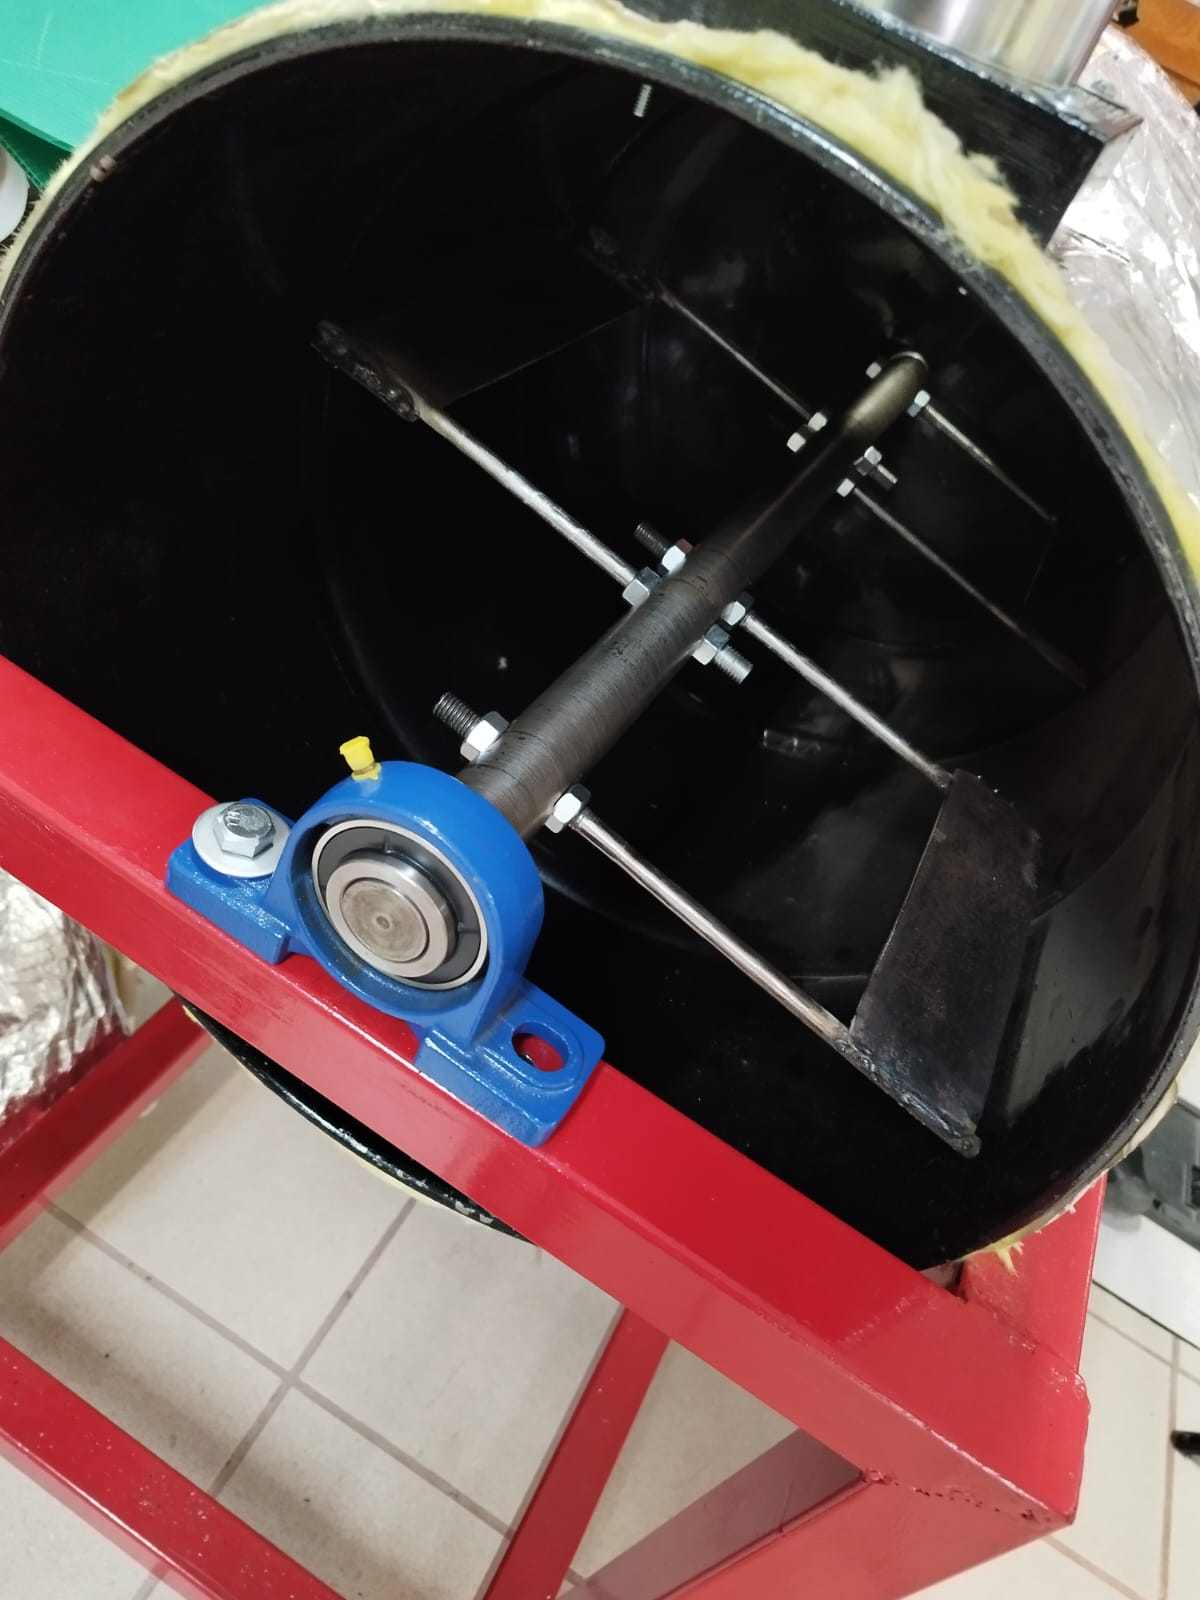
\includegraphics[scale=0.2]{images/Capitulo_Imple/S7/palas_dentro.jpeg}
            \caption{Instalación del eje de aireación dentro del contenedor}
            \label{fg:palas_dentro}
 \end{figure}
 
 \clearpage
Ya con el contenedor instalado dentro la estructura, se realizaron las conexiones entre los elementos de ventilación y trituración, para lo cual, se realizaron perforaciones sobre el contenedor, donde se instalaron y atornillaron las piezas necesarias para sostener los elementos de cada subsistema.

En una de las partes, se coloco la base que sostiene el filtro de olores, la cual está atornillada en la parte final del contenedor, mientras que a la entrada, se coloca la base donde se conectan los conductos de PVC, provenientes del sistema de trituración. (Figura \ref{fg:Filtro_olores}) 

 \begin{figure}[h!]
            \centering
            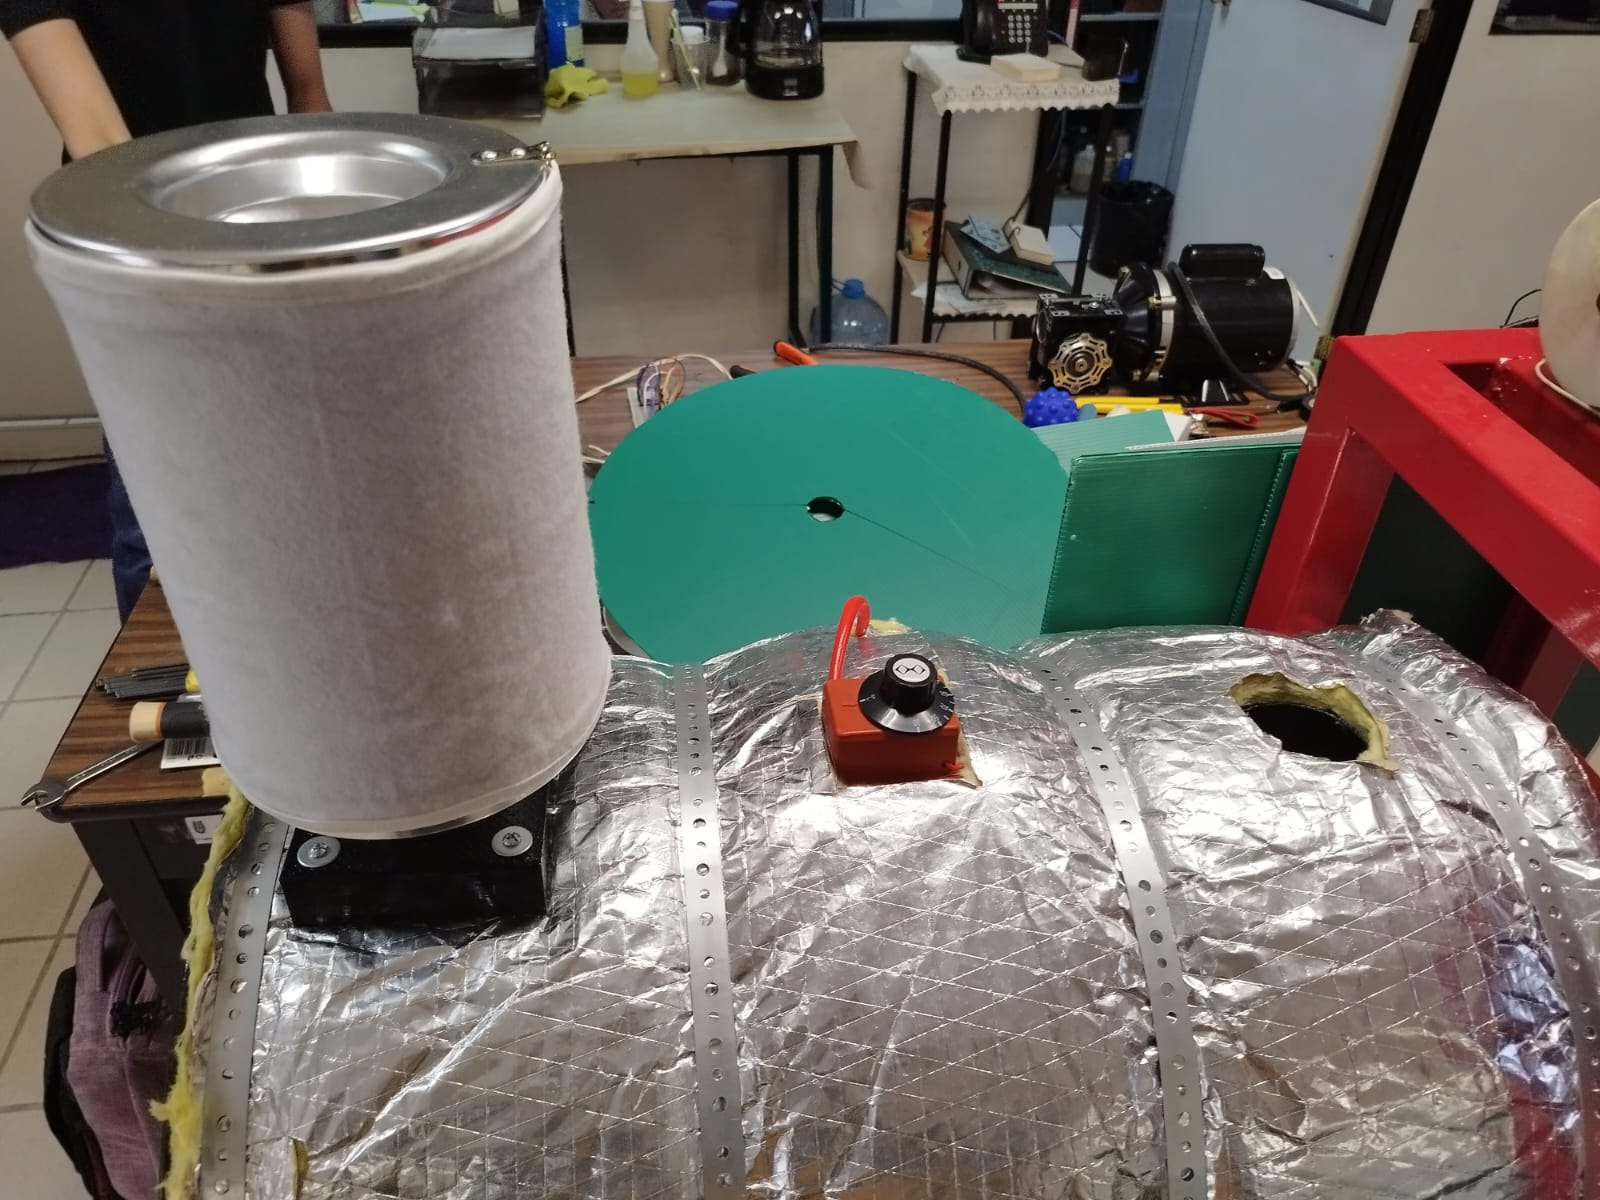
\includegraphics[scale=0.2]{images/Capitulo_Imple/S7/perfora.jpeg}
            \caption{Instalación del filtro de olores}
            \label{fg:Filtro_olores}
 \end{figure}
 
 \clearpage
 También se terminó por instalar el sistema de trituración sobre la estructura, atornillando el molino y su motor. Se ajustó la banda que transmite el movimiento entre el juego poleas y se colocaron los conductos de alimentación al contenedor. (Figura \ref{fg:Instalacion_triturac})

  \begin{figure}[h!]
            \centering
            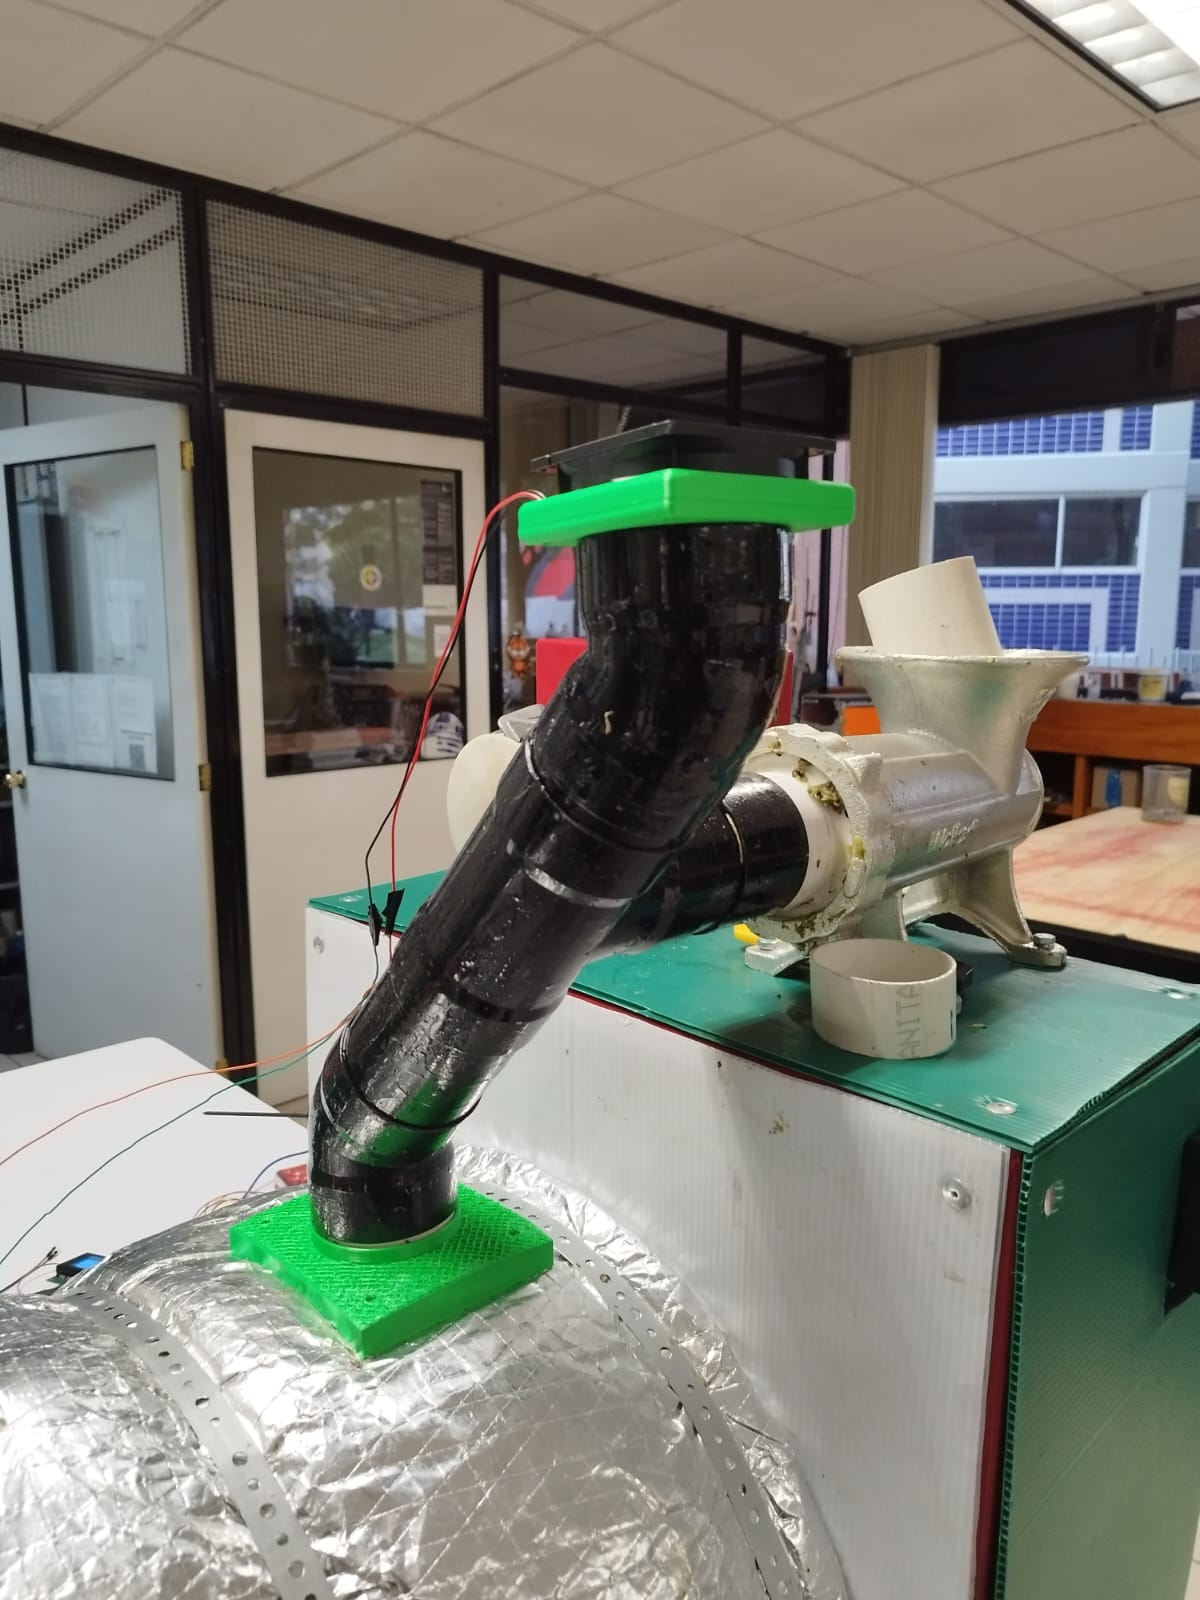
\includegraphics[scale=0.2]{images/Capitulo_Imple/S7/Sal_trituracion.jpeg}
            \caption{Sistema de trituración instalado}
            \label{fg:Instalacion_triturac}
 \end{figure}

\clearpage
Lo siguiente, fue colocar los sensores, recordando que el sensor de humedad se coloca en la parte superior del contenedor, sobre la perforación en la que se encuentra el filtro de olores y el de temperatura en la parte lateral, pegado a la pared del tanque.

Ya con la parte del eje y del contenedor colocada, se realizo del ensamble de los elementos de transmisión de movimiento del eje de aireación, el cual consta del motor eléctrico, el motor-reductor y el juego de poleas, con su respectiva banda. (Figura \ref{fg:Sist_trans_ints})

 \begin{figure}[h!]
            \centering
            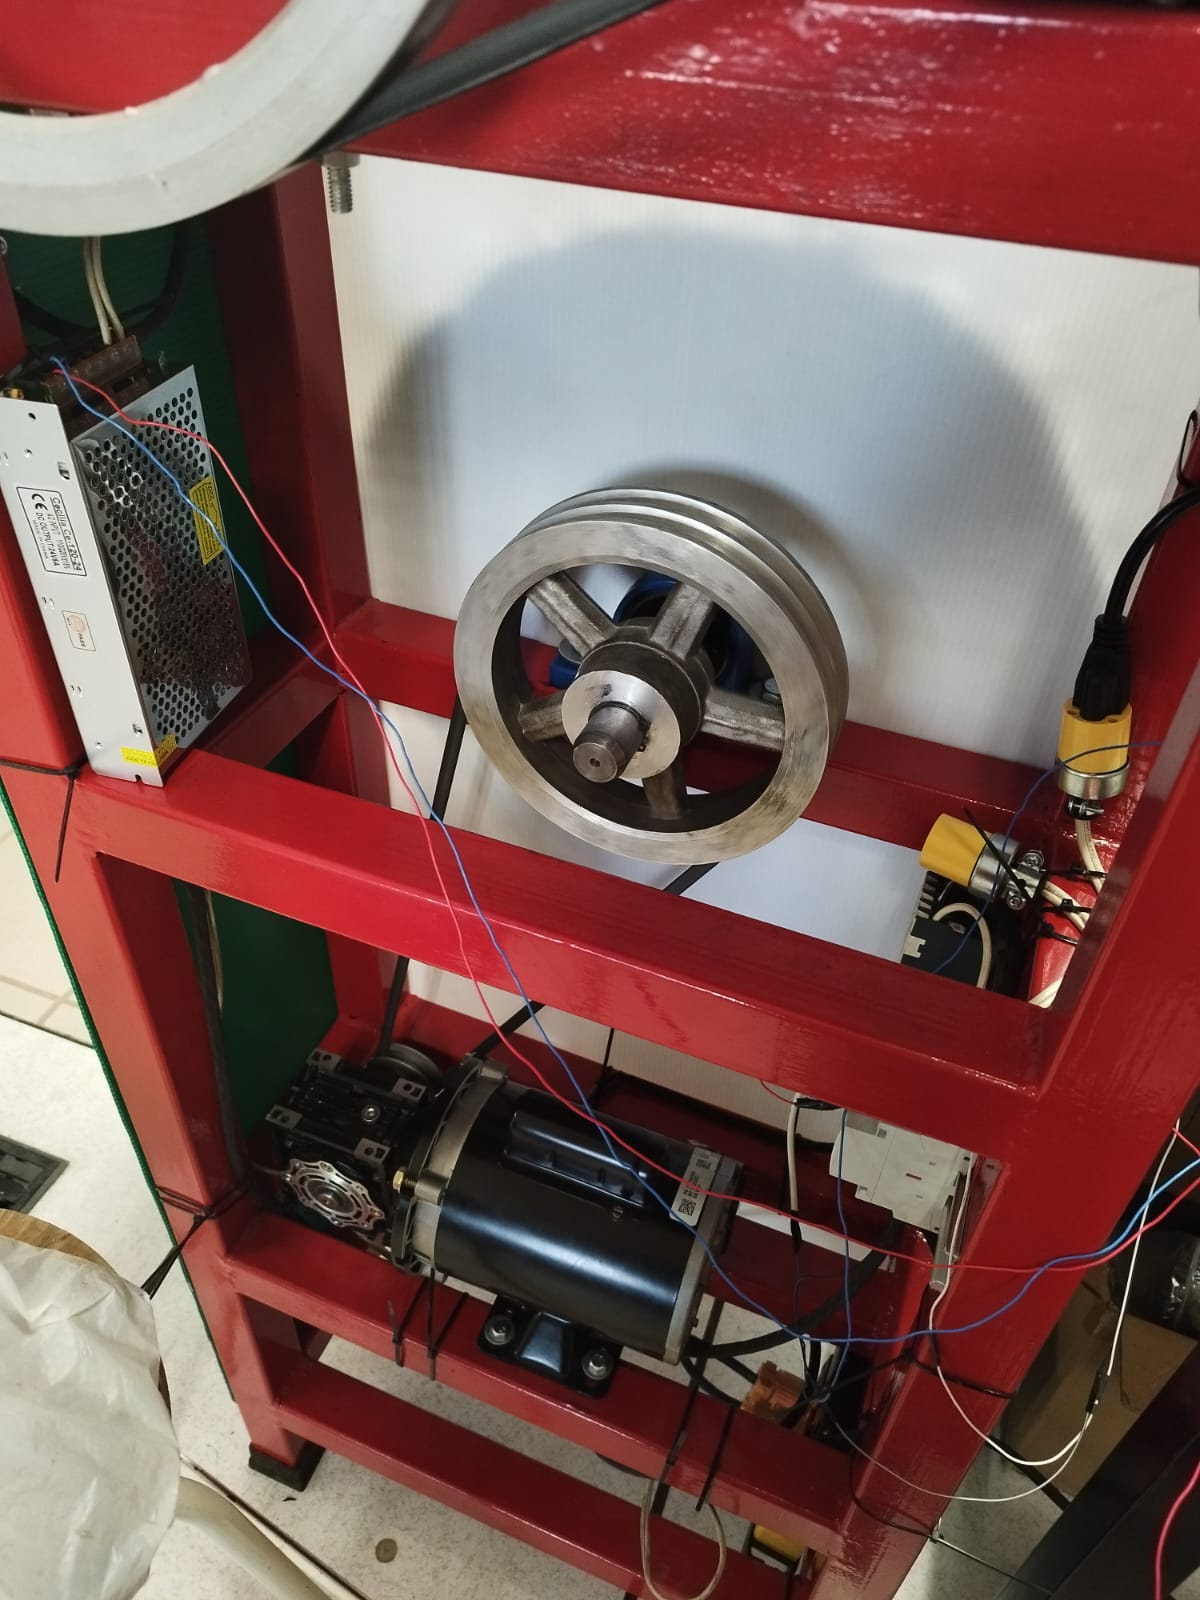
\includegraphics[scale=0.2]{images/Capitulo_Imple/S7/motor.jpeg}
            \caption{Sistema de transmisión instalado}
            \label{fg:Sist_trans_ints}
 \end{figure}

\clearpage
Al final, se colocaron todos los sistemas de control del dispositivo, colocando los contactores en el riel para la activación de los diferentes actuadores eléctricos, así como el montaje de la interfaz a un costado de la estructura. (Figura \ref{fg:Instal_contac})

 \begin{figure}[h!]
            \centering
            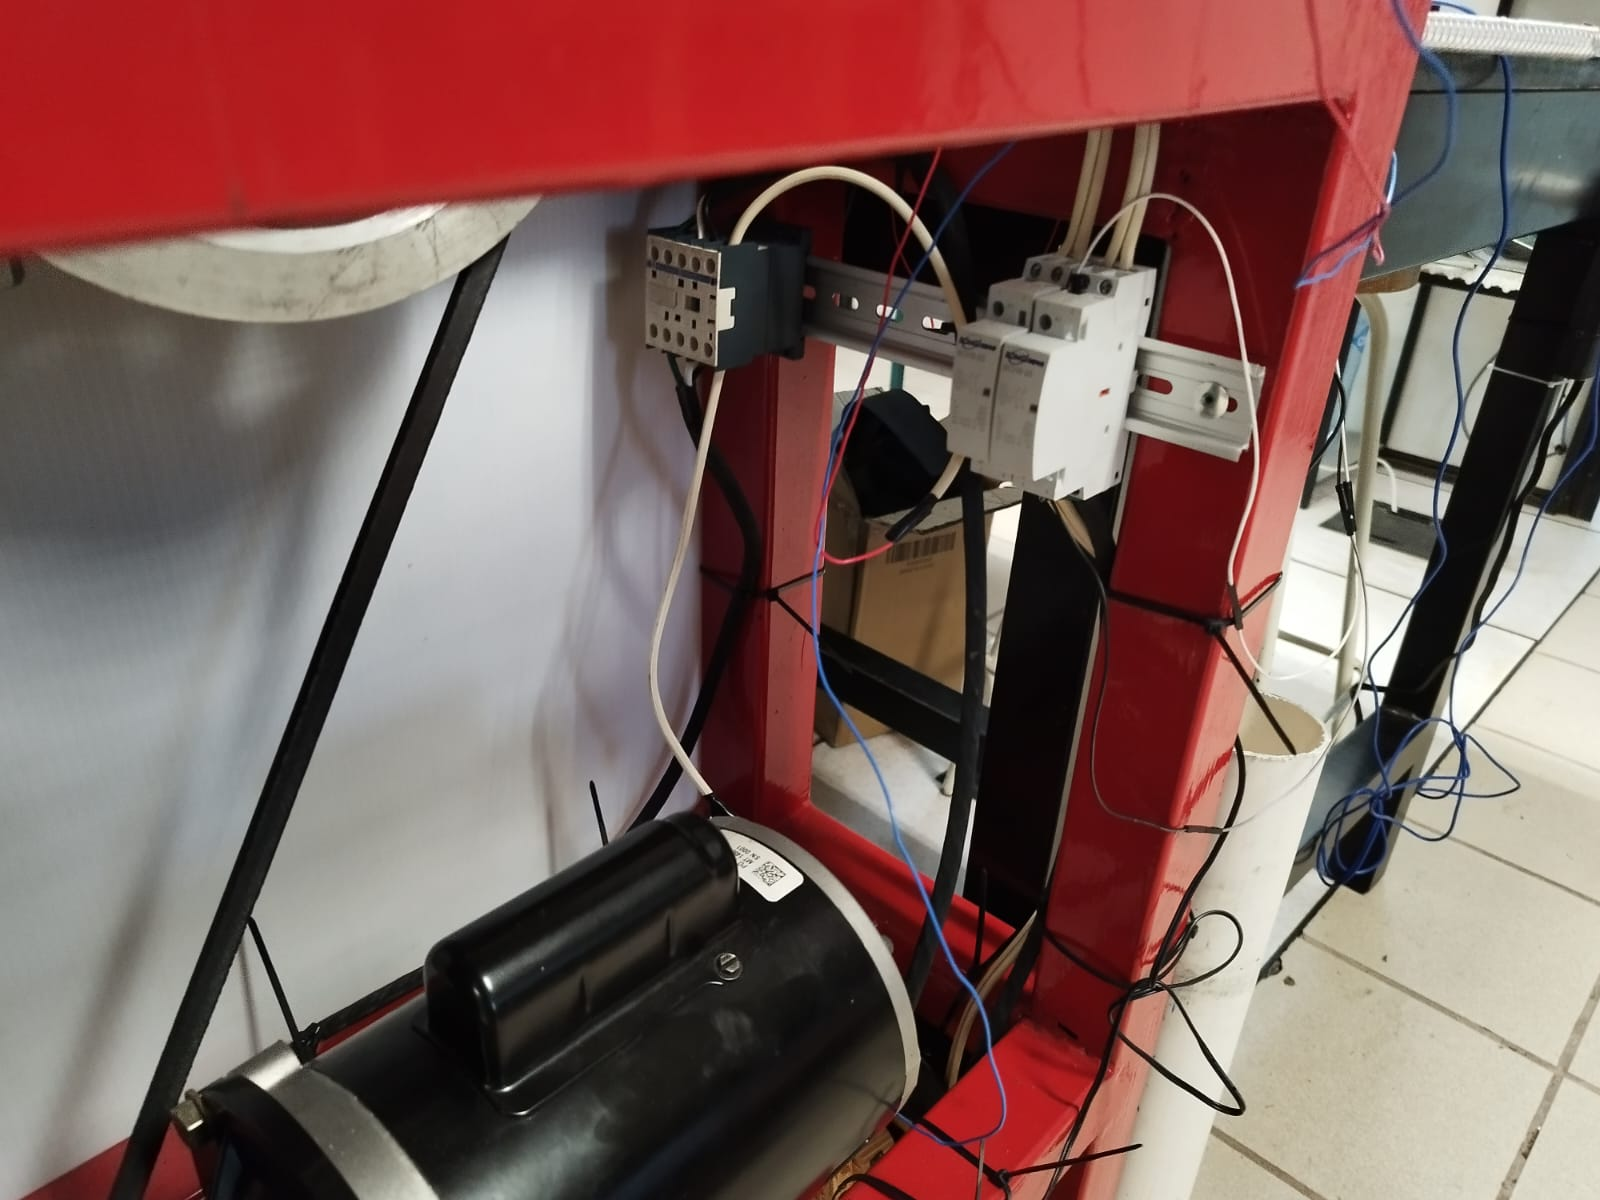
\includegraphics[scale=0.2]{images/Capitulo_Imple/S7/cableado.jpeg}
            \caption{Contantores instalados}
            \label{fg:Instal_contac}
 \end{figure}

De igual forma se colocaron laminas de plástico, encargadas de aislar los elementos mecánicos, eléctricos y electrónicos del sistema, para evitar que estén en contacto directo con el usuario o con líquidos que se puedan presentar durante las etapas del proceso.

\clearpage
Ya con el sistema armado, se realizaron las pruebas necesarias para observar su funcionamiento y realizar los ajustes necesarios para su integración y funcionamiento completo (Figura \ref{fg:sistema integrado})

 \begin{figure}[h!]
            \centering
            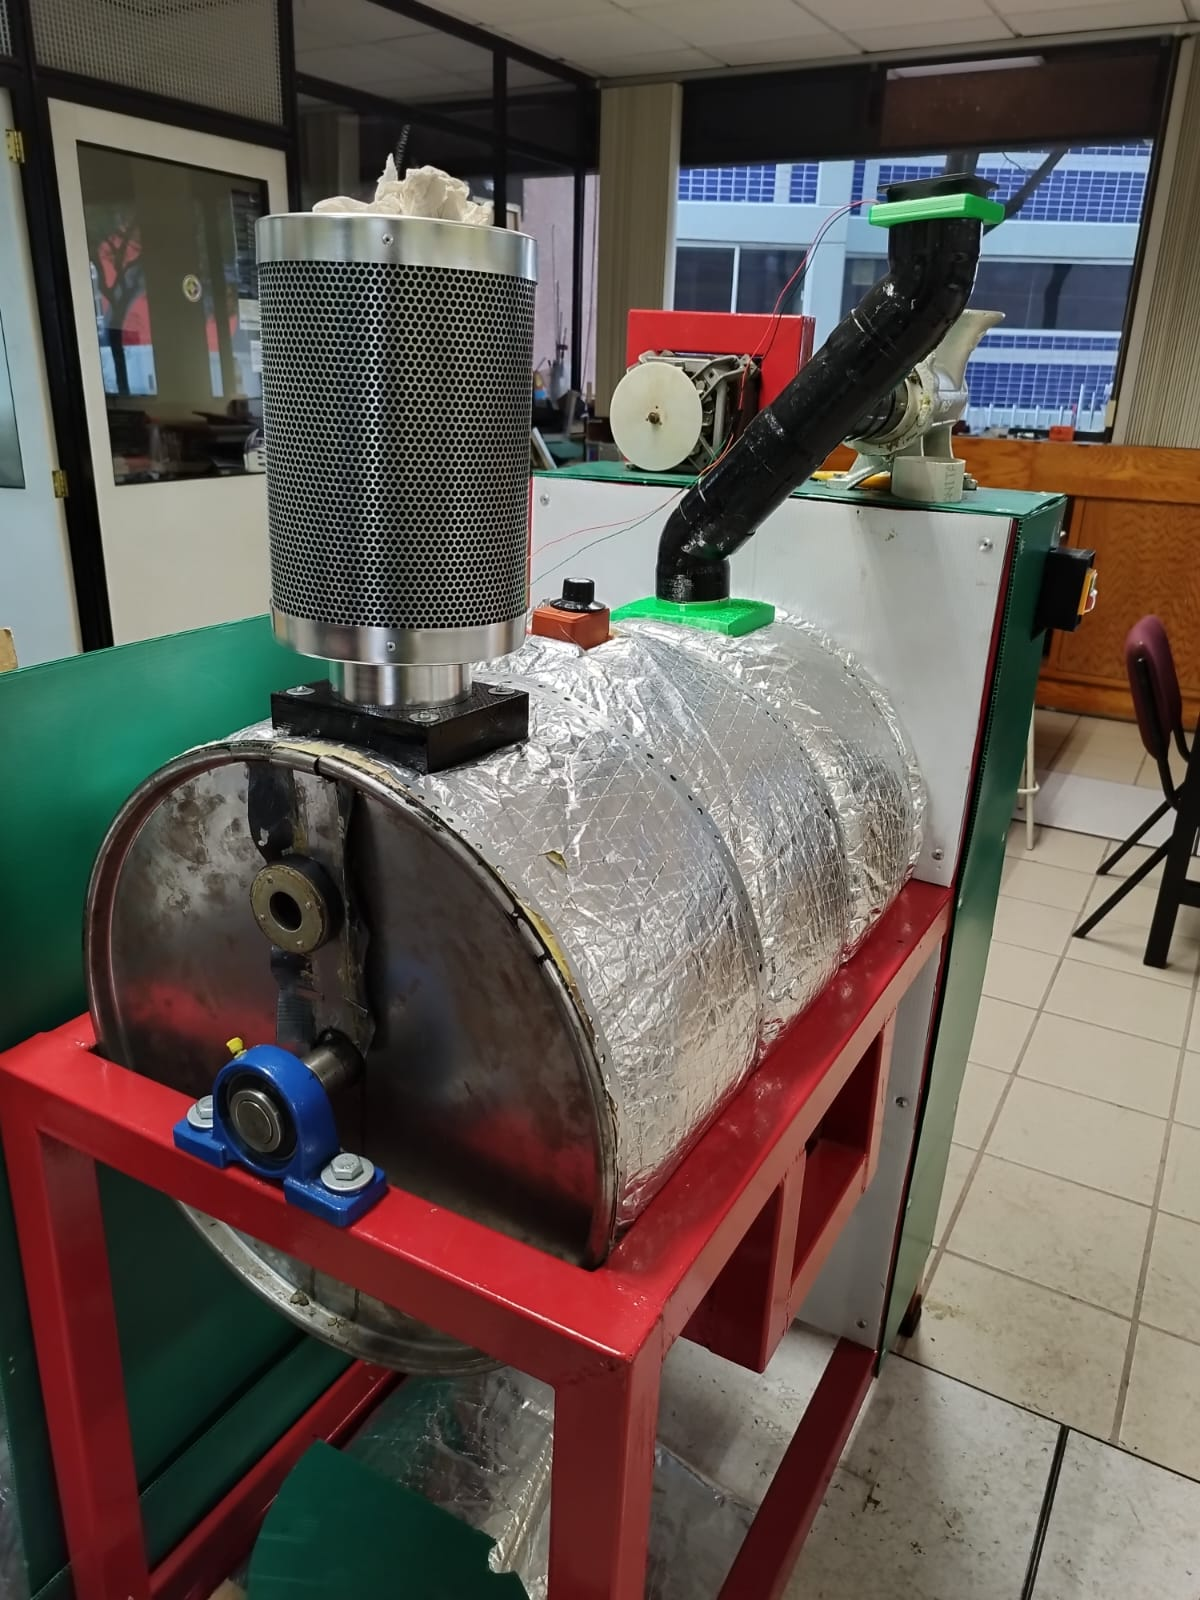
\includegraphics[scale=0.2]{images/Capitulo_Imple/S7/sistema_integrado.jpeg}
            \caption{Muestra del sistema de compostaje completo}
            \label{fg:sistema integrado}
 \end{figure}

 \clearpage

\textbf{Validación del sistema mecatrónico}

Para validar el funcionamiento del sistema mecatrónico, fue necesario llevar a cabo diversas pruebas de ciclo completo. Al momento de elaborar este reporte, se han efectuado seis pruebas, cuyos resultados han sido satisfactorios en su mayoría.

\textbf{\textit{Primera prueba}}

Esta prueba se realizó con una cantidad de 6 kg de desechos, entre los cuales se encontraban restos de zanahorias, lechugas, papas, tallos de cebolla, toronja, ajos y cáscara de melón y sandía.

\begin{figure}[h]
    \centering
    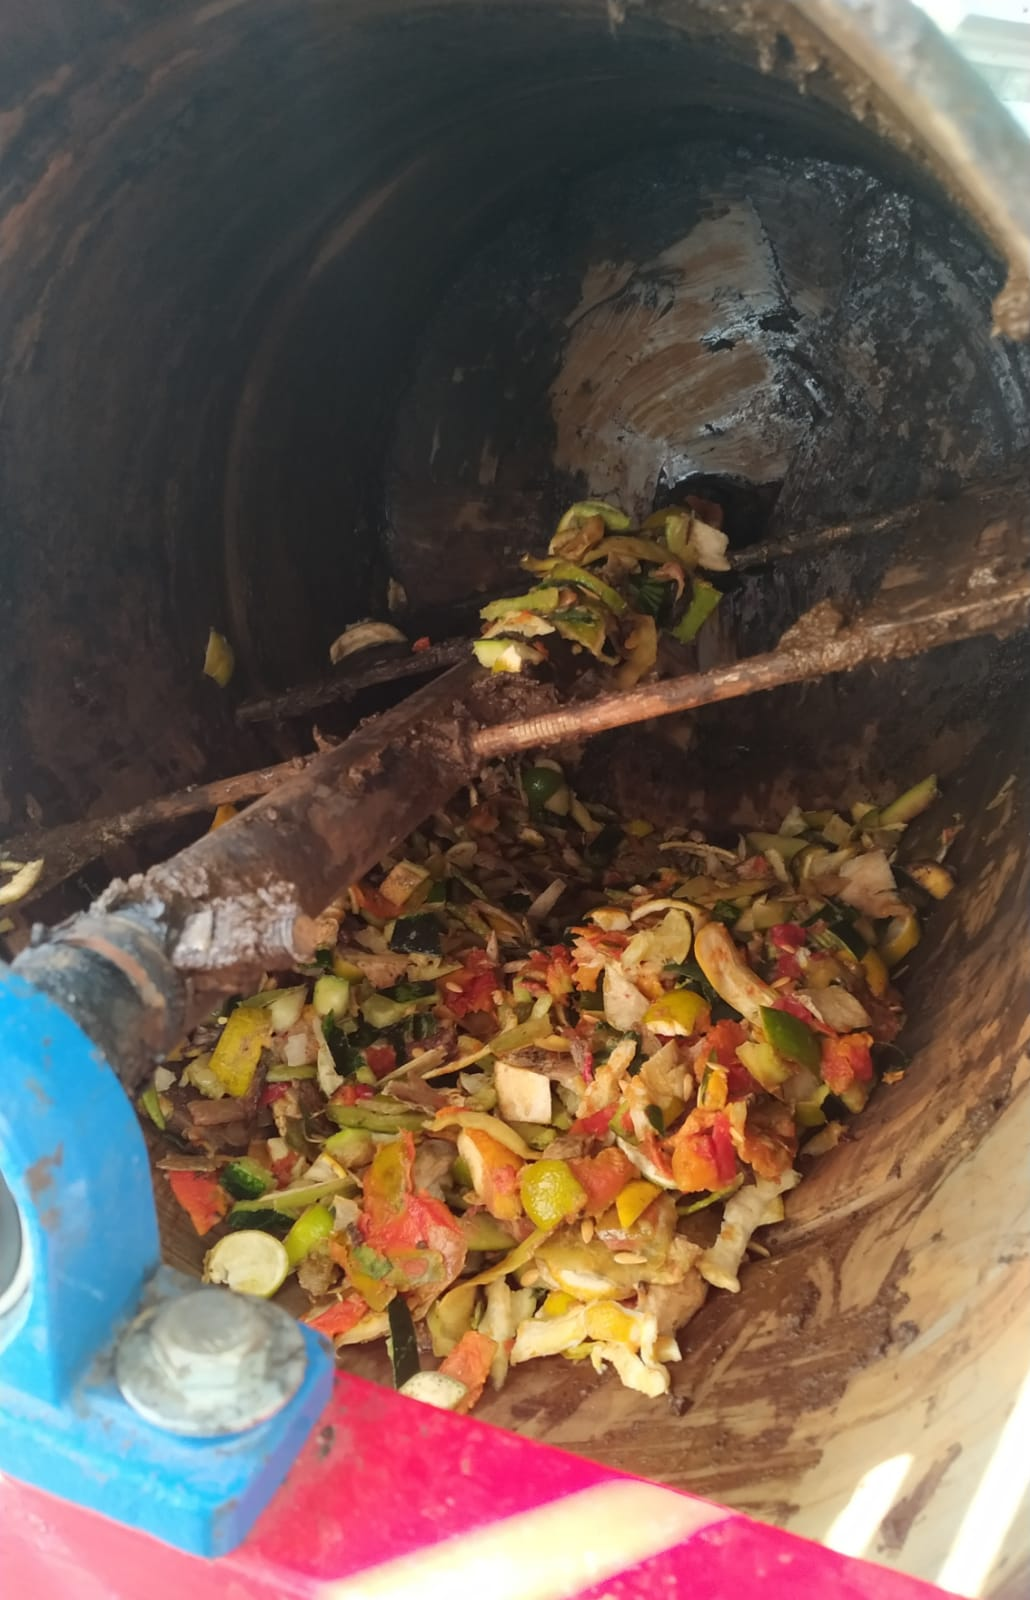
\includegraphics[scale=0.15]{images/Pruebas/Pruebas_compost/carga1.jpeg}
    \caption{Carga primera prueba}
    \label{fg:carga1}
\end{figure}
\clearpage

Esta prueba se realizó dentro del laboratorio de Trabajo Terminal 1, buscando completar un ciclo continuo de trabajo de 72 horas a lo largo de un fin de semana. Sin embargo, esta prueba se vio afectada por un corte de energía, el cual interrumpió el ciclo de trabajo después de un tiempo aproximado de 50 horas, cuando se encontraba en la segunda fase del crecimiento bacteriano.

Por lo que la materia que se logró obtener aún tenía algunos trozos reconocibles de verduras. A su vez, los desechos ya empezaban a adquirir un color marrón y se podían deshacer al contacto.

A pesar de tener un estado avanzado de descomposición, desprendían un olor agradable. También se encontraron con una humedad muy alta, siendo resultado de todos los líquidos lixiviados que se generaron durante el proceso y que quedaron atrapados en el contenedor.

\begin{figure}[h]
    \centering
    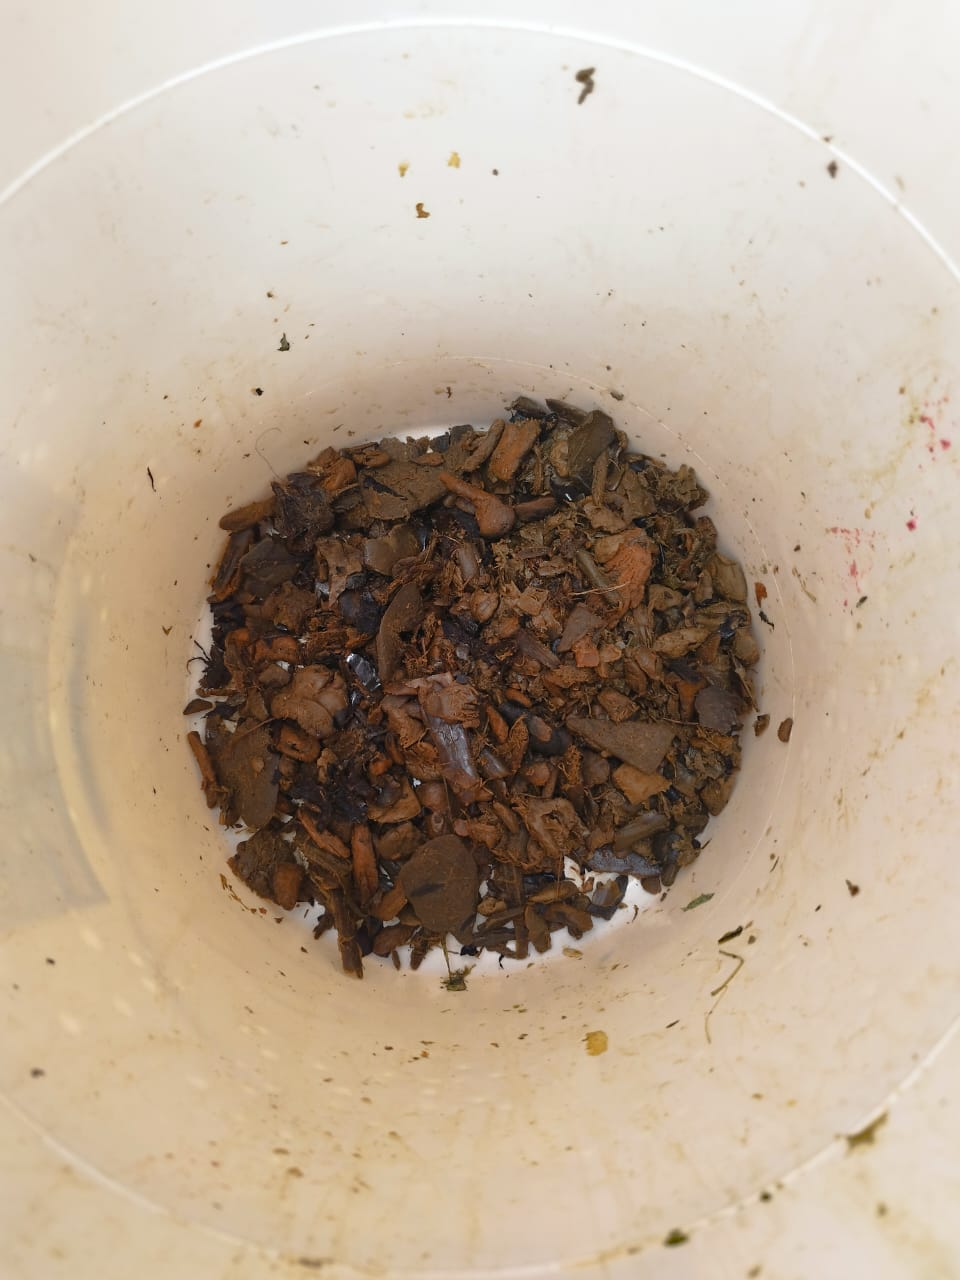
\includegraphics[scale=0.15]{images/Capitulo_Imple/S7/Val/Prueba1.jpeg}
    \caption{Primera muestra de composta obtenida}
    \label{fg:muestra1}
\end{figure}
\clearpage

\textbf{\textit{Segunda prueba}}

En esta segunda prueba se trabajó con 15 kg de residuos orgánicos, compuestos principalmente por desechos frutales, como melón, sandía y papaya, así como por residuos de verduras, entre los que se encontraban papa, jitomate y cebolla.

Para esta segunda prueba, se cambió el escenario de prueba, en donde se trasladó el dispositivo al anexo del laboratorio de Trabajo Terminal. Este espacio representa un área expuesta al aire libre, cubierta con láminas para evitar que se moje con la lluvia.

\begin{figure}[h]
    \centering
    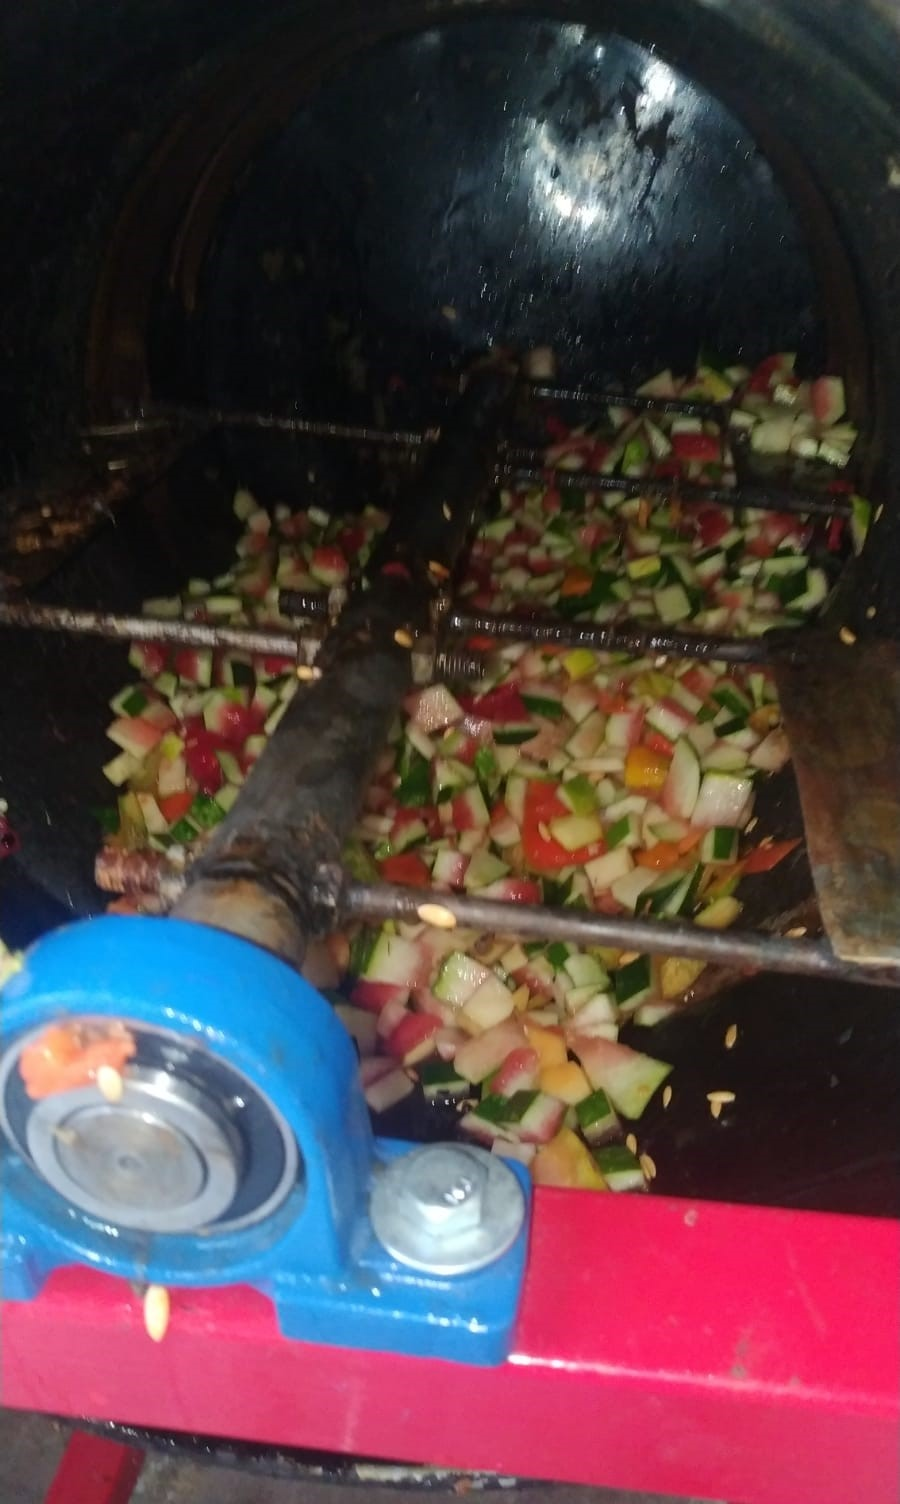
\includegraphics[scale=0.15]{images/Pruebas/Pruebas_compost/carga2.jpeg}
    \caption{Segunda carga}
    \label{fg:carga2}
\end{figure}
\clearpage

Esta prueba se hizo con una supervisión continua, ya que se realizó entre semana. Esta semana de pruebas contó con un clima muy frío que osciló entre los 8 °C y los 16 °C, por lo que se registraron mayores pérdidas de calor al interior del contenedor. De esta manera, el sistema para elevar la temperatura se mantuvo encendido más tiempo y representó un mayor consumo de energía.

A pesar de esto, se logró mantener un ciclo completo de 72 horas, por lo que, al final, fue posible obtener una mezcla más homogénea, con un peso de 6.4 kg. Esta materia ya contaba con un color marrón más intenso y un olor agradable, como a ponche de frutas. De igual manera, presentaba una consistencia bastante húmeda; por tal motivo, se procedió a realizar otro ciclo de 24 horas con el fin de eliminar el exceso de agua. Sin embargo, el resultado no distaba de la muestra obtenida previamente, ya que la mezcla seguía presentando una cantidad considerable de agua.

\begin{figure}[h]
    \centering
    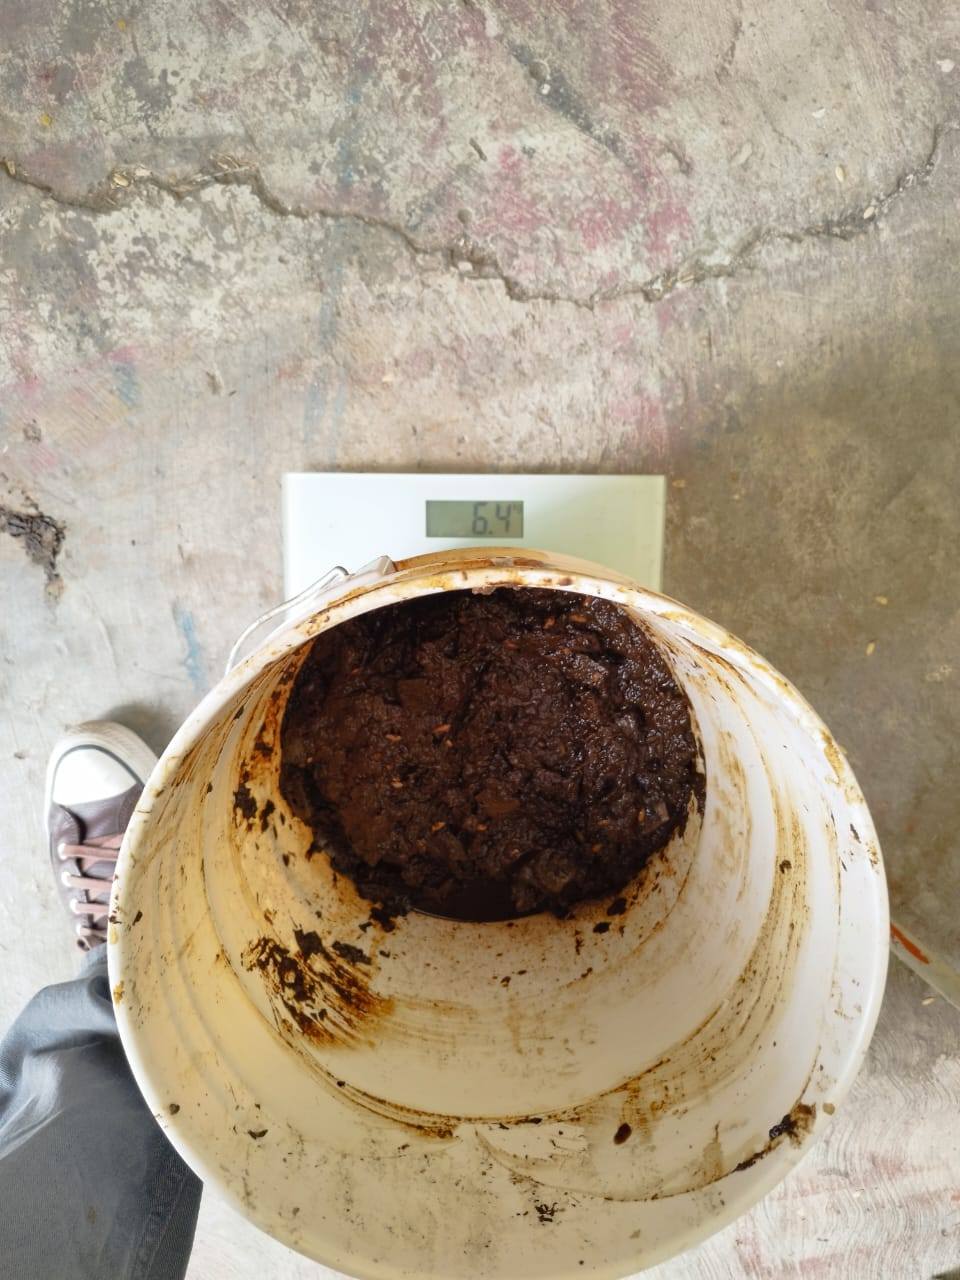
\includegraphics[scale=0.15]{images/Capitulo_Imple/S7/Val/Prueba2.jpeg}
    \caption{Segunda muestra de composta obtenida}
    \label{fg:muestra2}
\end{figure}
\clearpage

\textbf{\textit{Tercera prueba}}

Para la tercera prueba se emplearon cerca de 13.8 kg de residuos. De igual manera que en los procesos anteriores, se utilizaron desechos frutales, como melón, sandía y papaya, y también se emplearon desechos provenientes de verduras, como papa, jitomate y zanahoria.

Sin embargo, en esta prueba se trituró la totalidad de los desechos, obteniendo partículas de aproximadamente 3 mm de tamaño. Como se puede observar en la siguiente imagen, la mezcla presenta una apariencia más homogénea, debido a que los residuos triturados adquieren prácticamente una misma tonalidad naranja. Por otro lado, es importante mencionar que las frutas y verduras utilizadas en esta prueba presentaban una apariencia seca antes de la trituración, por lo que se observó una menor cantidad de líquidos durante este proceso.

\begin{figure}[h]
    \centering
    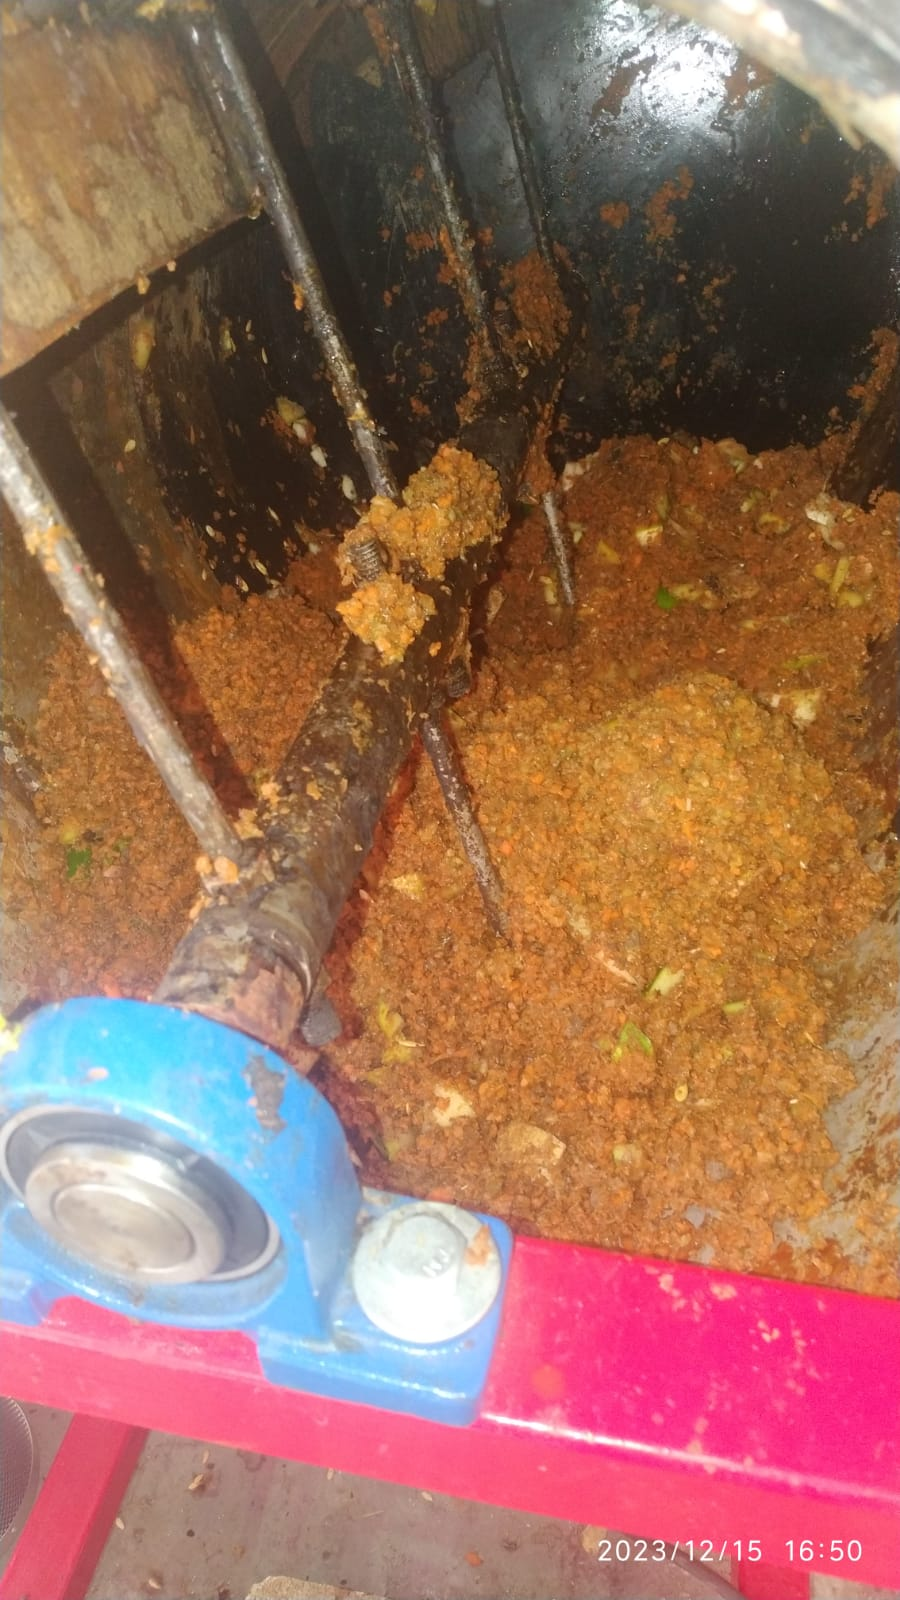
\includegraphics[scale=0.15]{images/Pruebas/Pruebas_compost/carga3.jpeg}
    \caption{Tercera prueba carga}
    \label{fg:carga3}
\end{figure}

Esta prueba duró 72 horas, obteniéndose 5.6 kg. Como se puede observar en la siguiente imagen, presenta una apariencia más cercana a la tierra empleada para las macetas, pues la partícula es más fina y presenta un color café obscuro además de un olor agradable, como a durazno. Otra característica a notar es que la cantidad de agua es mínima. Además, al apretar la mezcla con la mano y soltarla, esta se deshace como si se tratara de tierra. Los elementos de mayor tamaño fueron cáscaras que no pasaron por el triturador.

\begin{figure}[h]
    \centering
    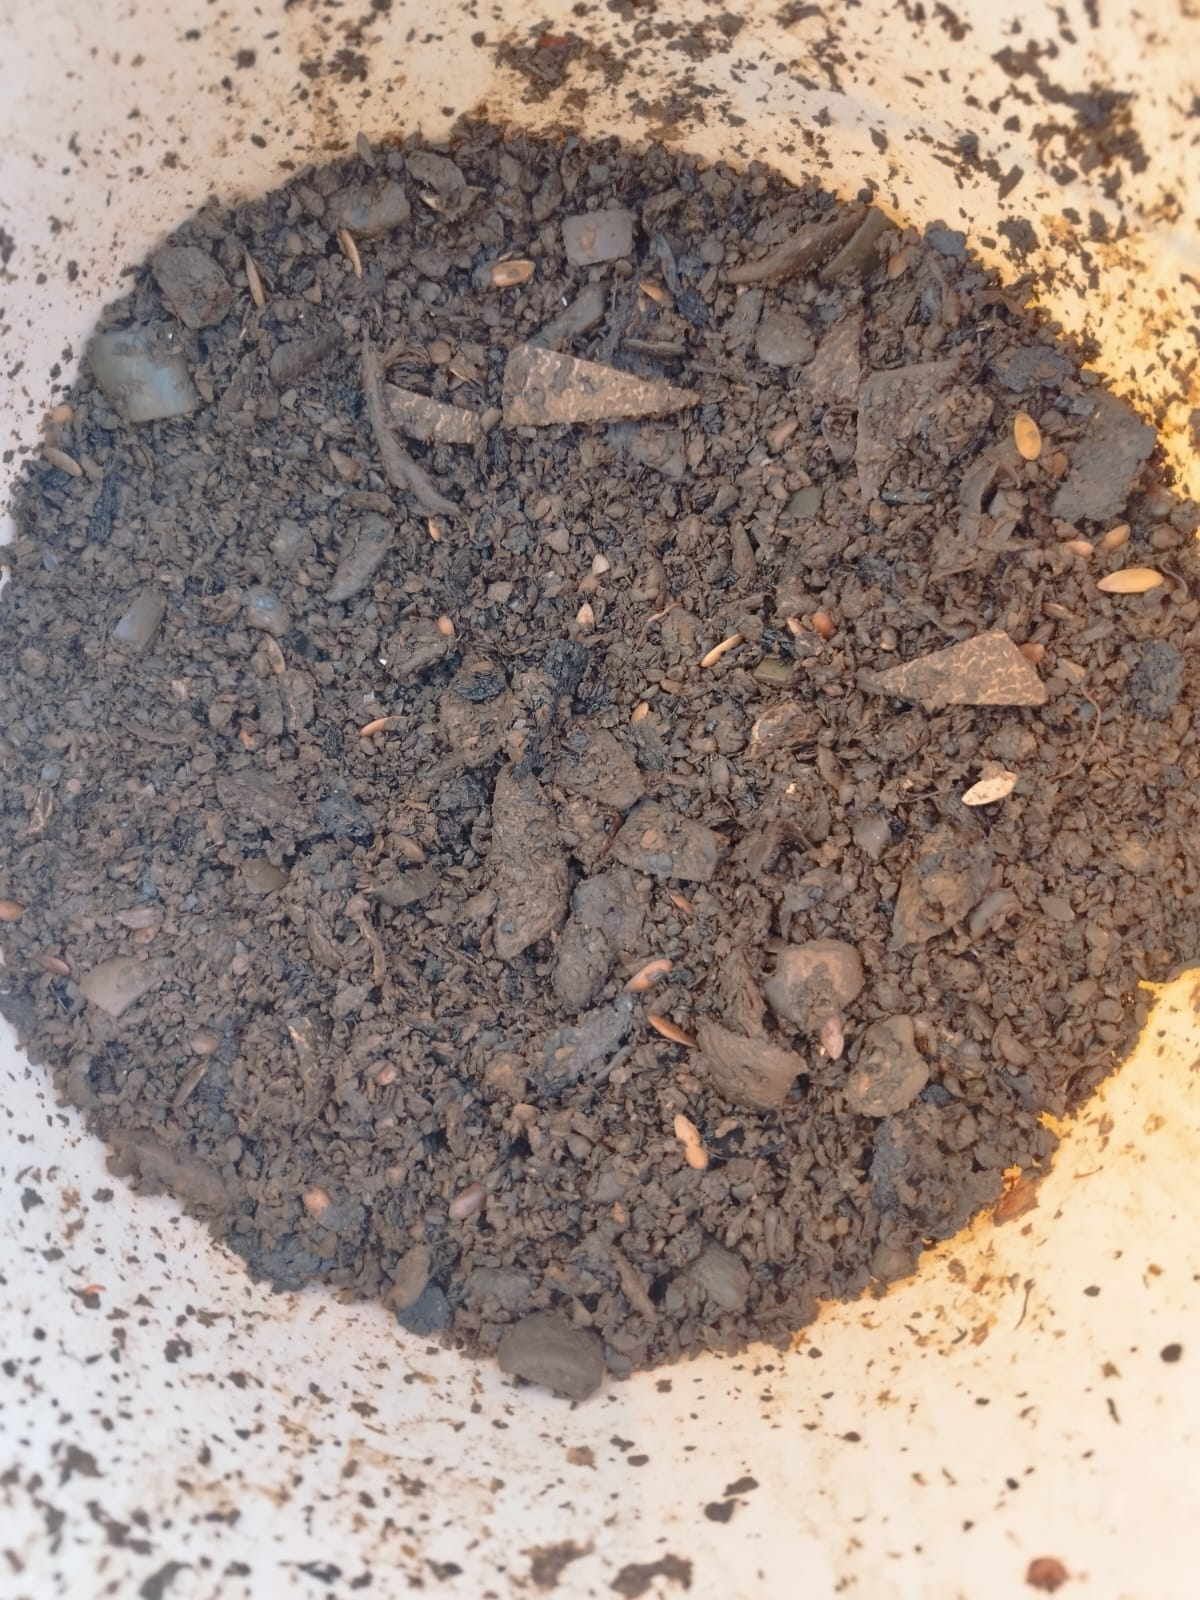
\includegraphics[scale=0.15]{images/Pruebas/Pruebas_compost/descarga3.jpeg}
    \caption{Tercera prueba descarga}
    \label{fg:descarga3}
\end{figure}

\textbf{\textit{Cuarta prueba}}

En esta prueba se introdujeron aproximadamente 14.1 kg de desechos, compuestos por frutas como sandía, melón y papaya, así como por verduras, entre las que se encontraban zanahoria y papa. Del total de los residuos, la mitad fue triturada, mientras que la otra mitad se introdujo únicamente picada. El proceso se mantuvo durante un ciclo de 72 horas, al término del cual se obtuvieron 6.1 kg de compost. Como se puede observar en la siguiente imagen, la mezcla presenta una apariencia homogénea y un nivel de humedad moderado. Asimismo, se percibe un olor agradable con características frutales.

\begin{figure}[h]
    \centering
    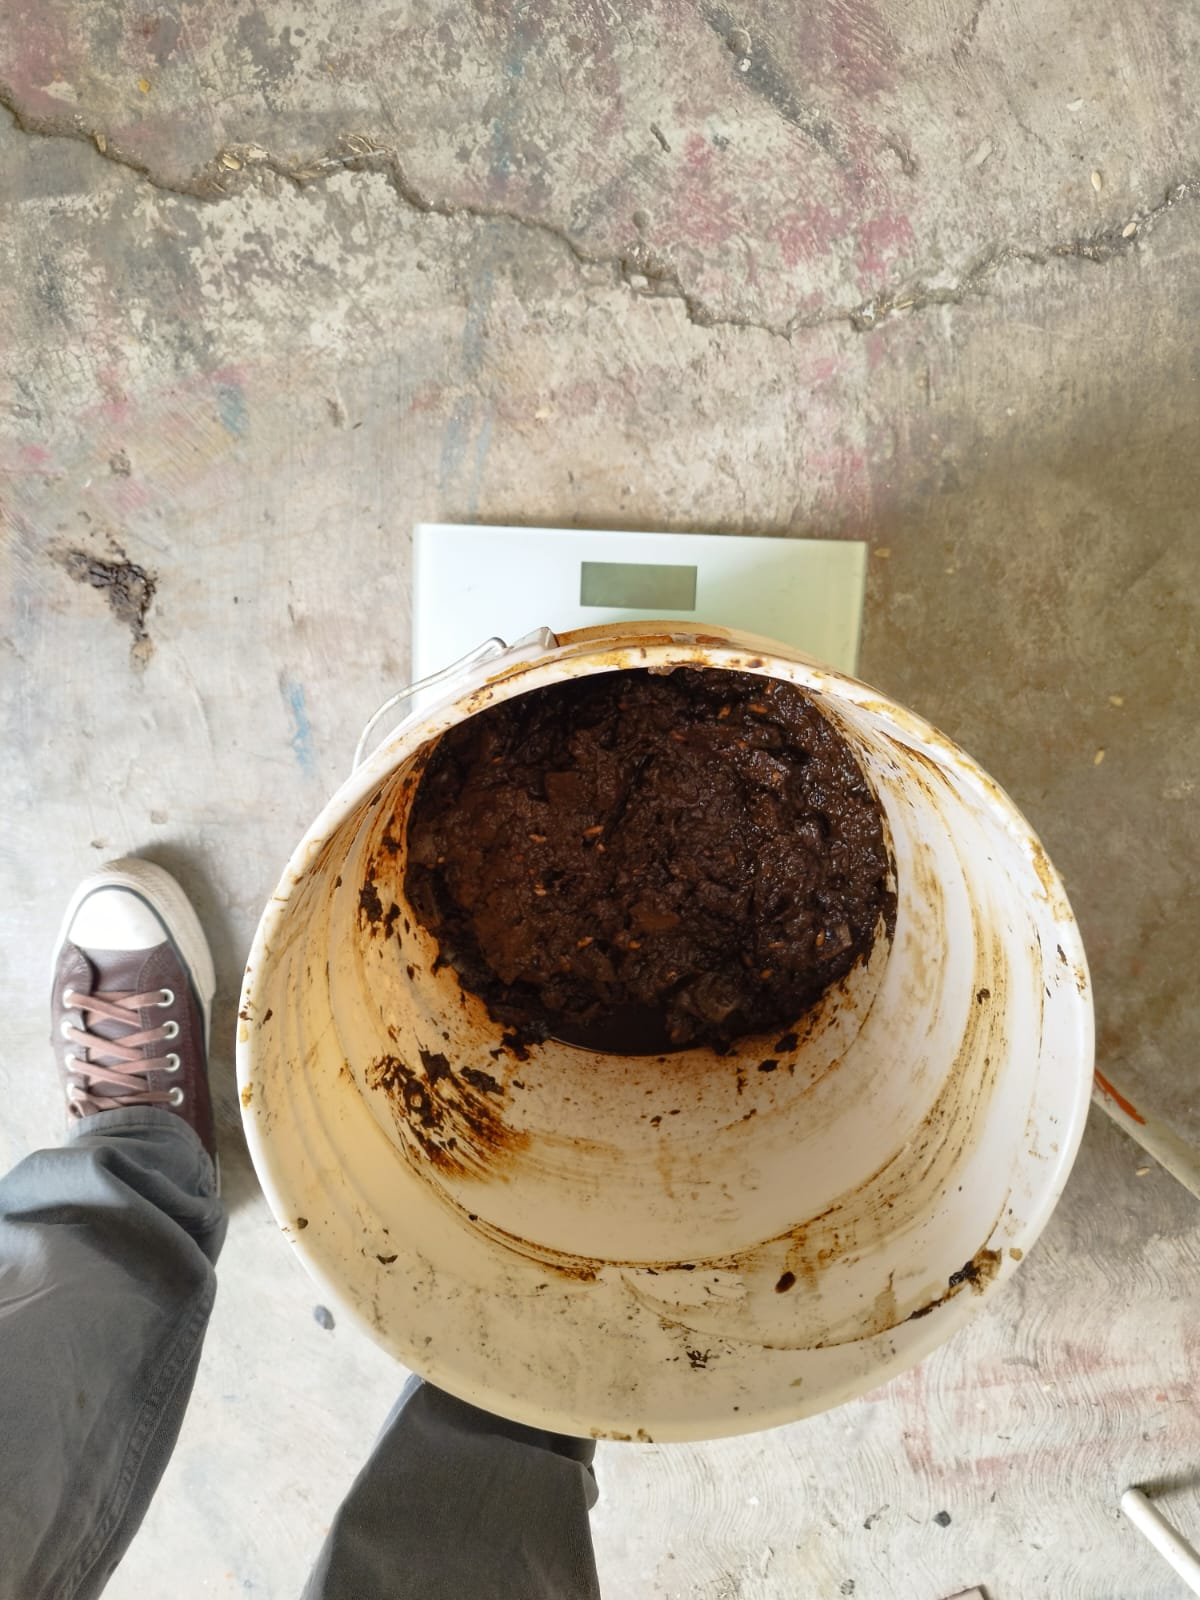
\includegraphics[scale=0.15]{images/Pruebas/Pruebas_compost/descarga4.jpeg}
    \caption{Cuarta prueba descarga}
    \label{fg:descarga4}
\end{figure}

\textbf{\textit{Quinta prueba}}

Cabe destacar, que en esta prueba se introdujo la mayor cantidad de desechos registrada para este proyecto, teniendo un total de 15.5 Kg de frutas y verduras. Para esta ocasión no se trituró la mezcla, sino que solamente se picó y se colocó en el contenedor.

\begin{figure}[h]
    \centering
    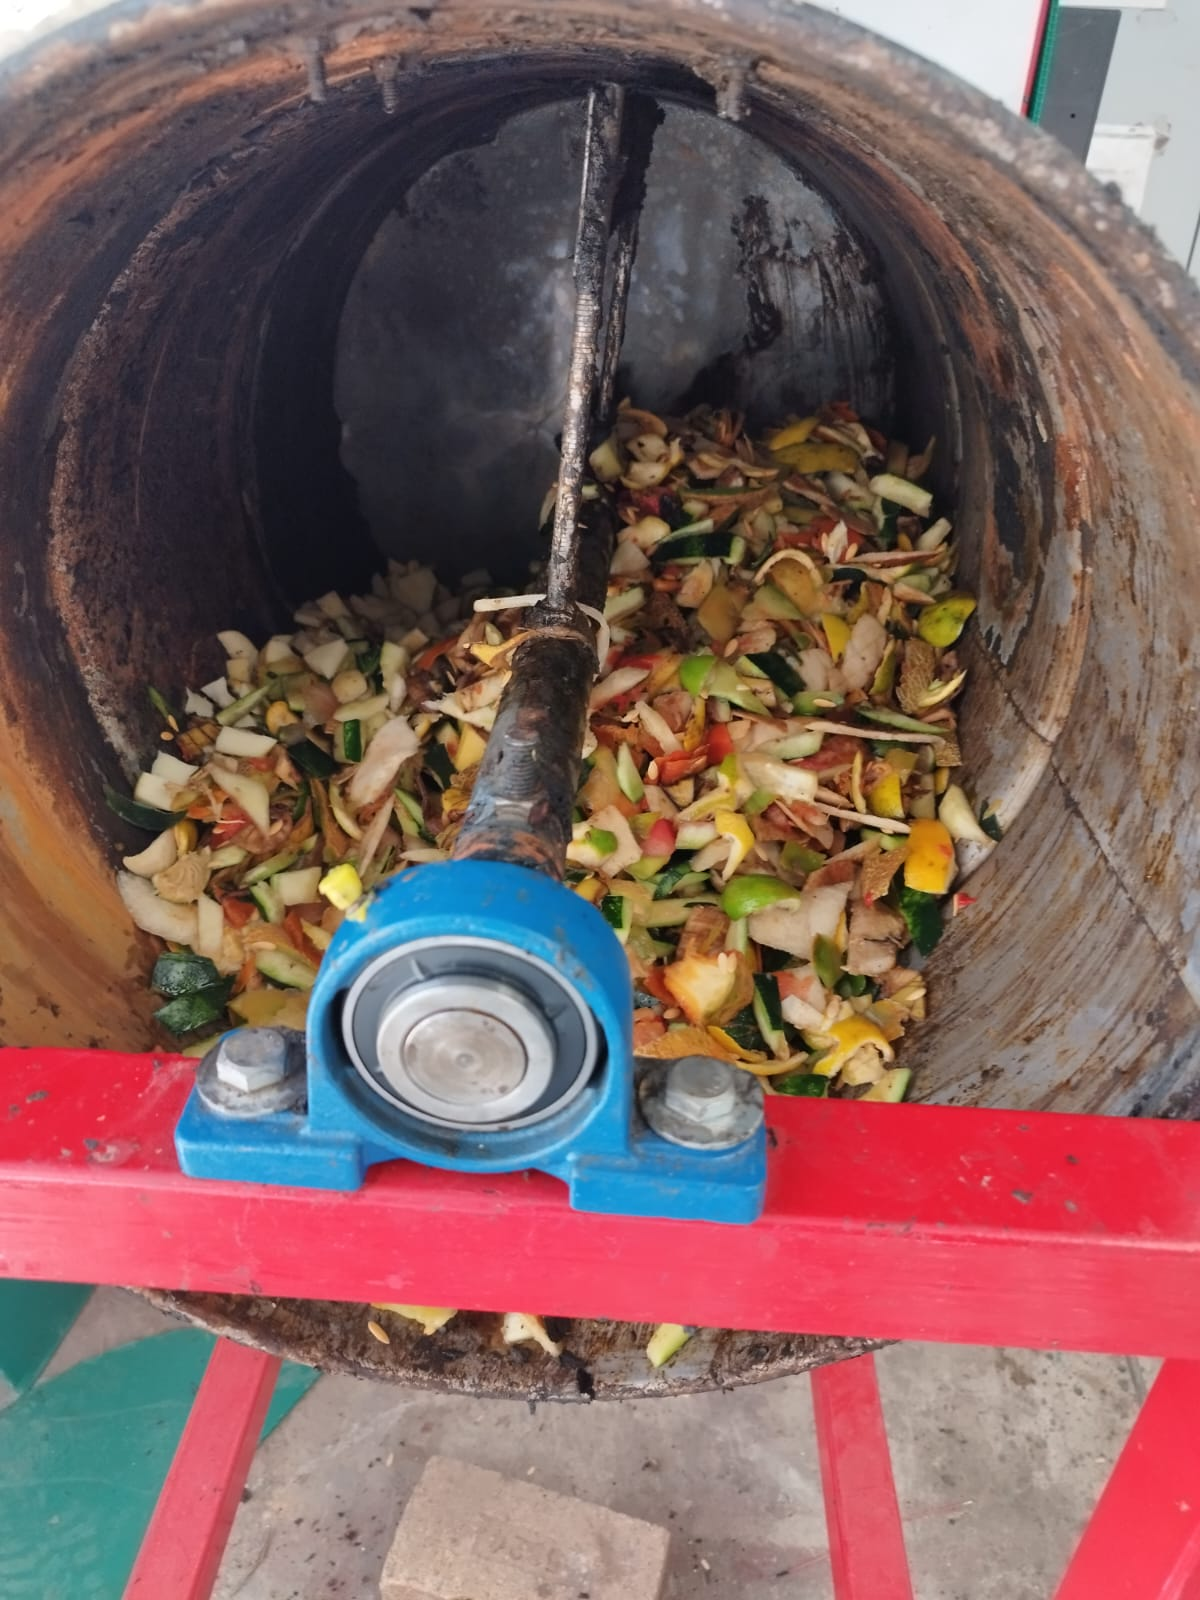
\includegraphics[scale=0.15]{images/Pruebas/Pruebas_compost/carga5.jpeg}
    \caption{Quinta prueba carga}
    \label{fg:carga5}
\end{figure}

Es importante señalar que la fruta y verdura eran frescas, conteniendo una gran cantidad de agua. Se hace hincapié en este detalle, pues a lo largo de estas pruebas se ha observado que el estado en el que ingresan los desechos influye en el resultado final. Como se puede observar en la siguiente imagen, la mezcla presenta una consistencia parecida al mole o al lodo, lo que indicaría que aún presenta un porcentaje de agua considerable. Por otro lado, se continúa obteniendo una mezcla homogénea de color café oscuro y de olor agradable. Al final de este intento se extrajeron 7.5 kg de compost.

\begin{figure}[h]
    \centering
    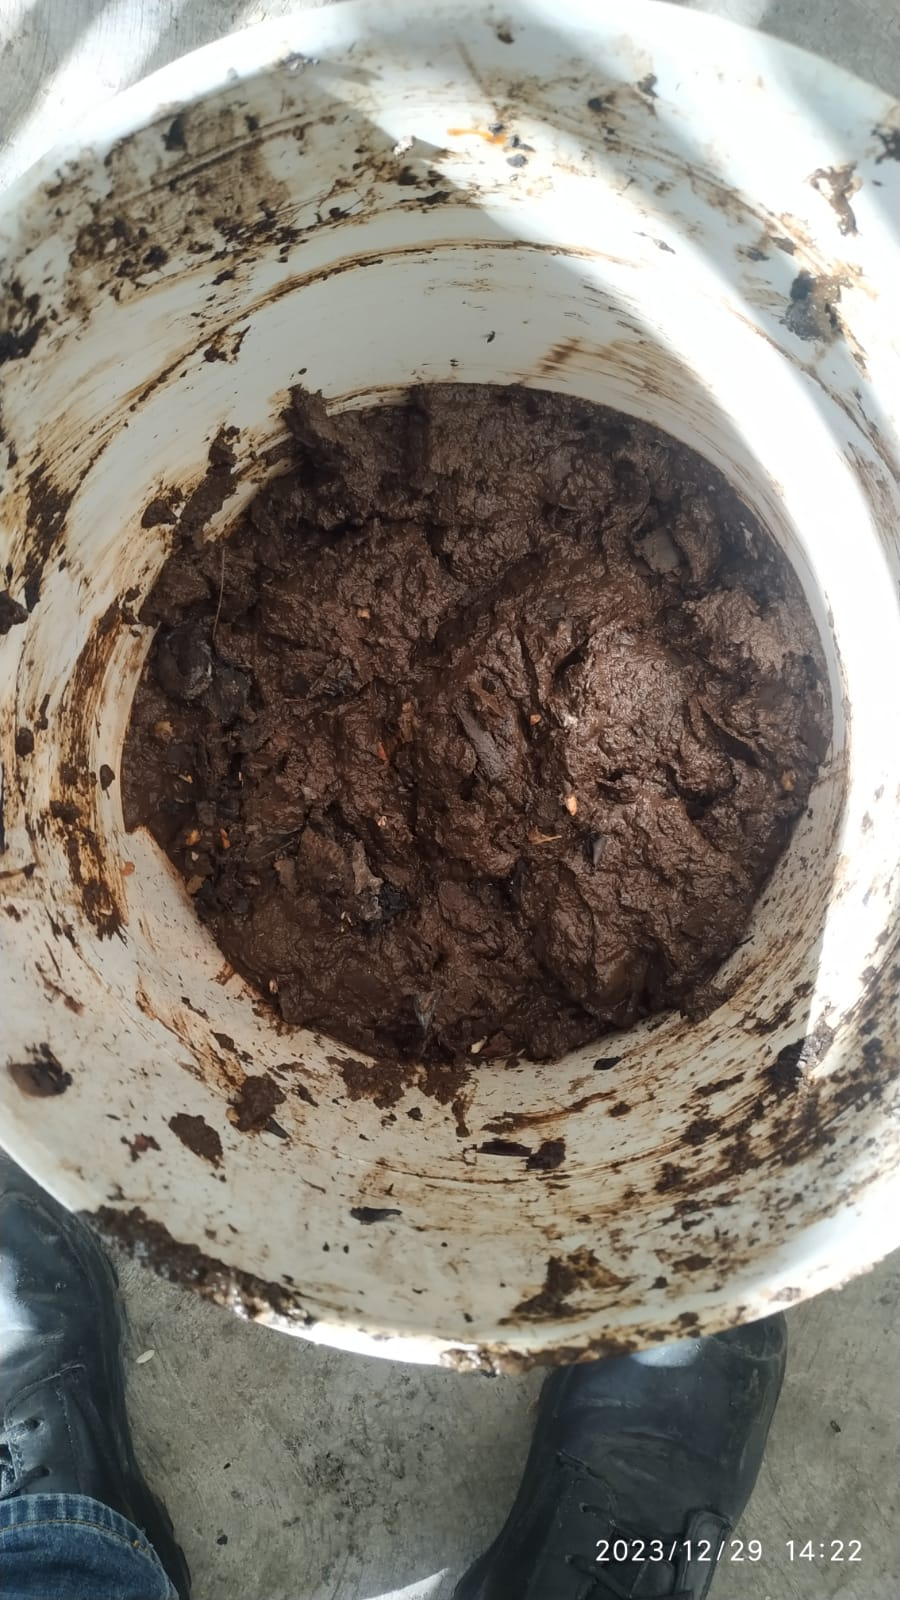
\includegraphics[scale=0.15]{images/Pruebas/Pruebas_compost/descarga5.jpeg}
    \caption{Quinta prueba descarga}
    \label{fg:descarga5}
\end{figure}

\textbf{\textit{Sexta prueba}}

Para la última prueba se introdujeron 7.2 kg de desperdicios entre fruta y verdura siendo de las pruebas con menor carga registrada.

\begin{figure}[h]
    \centering
    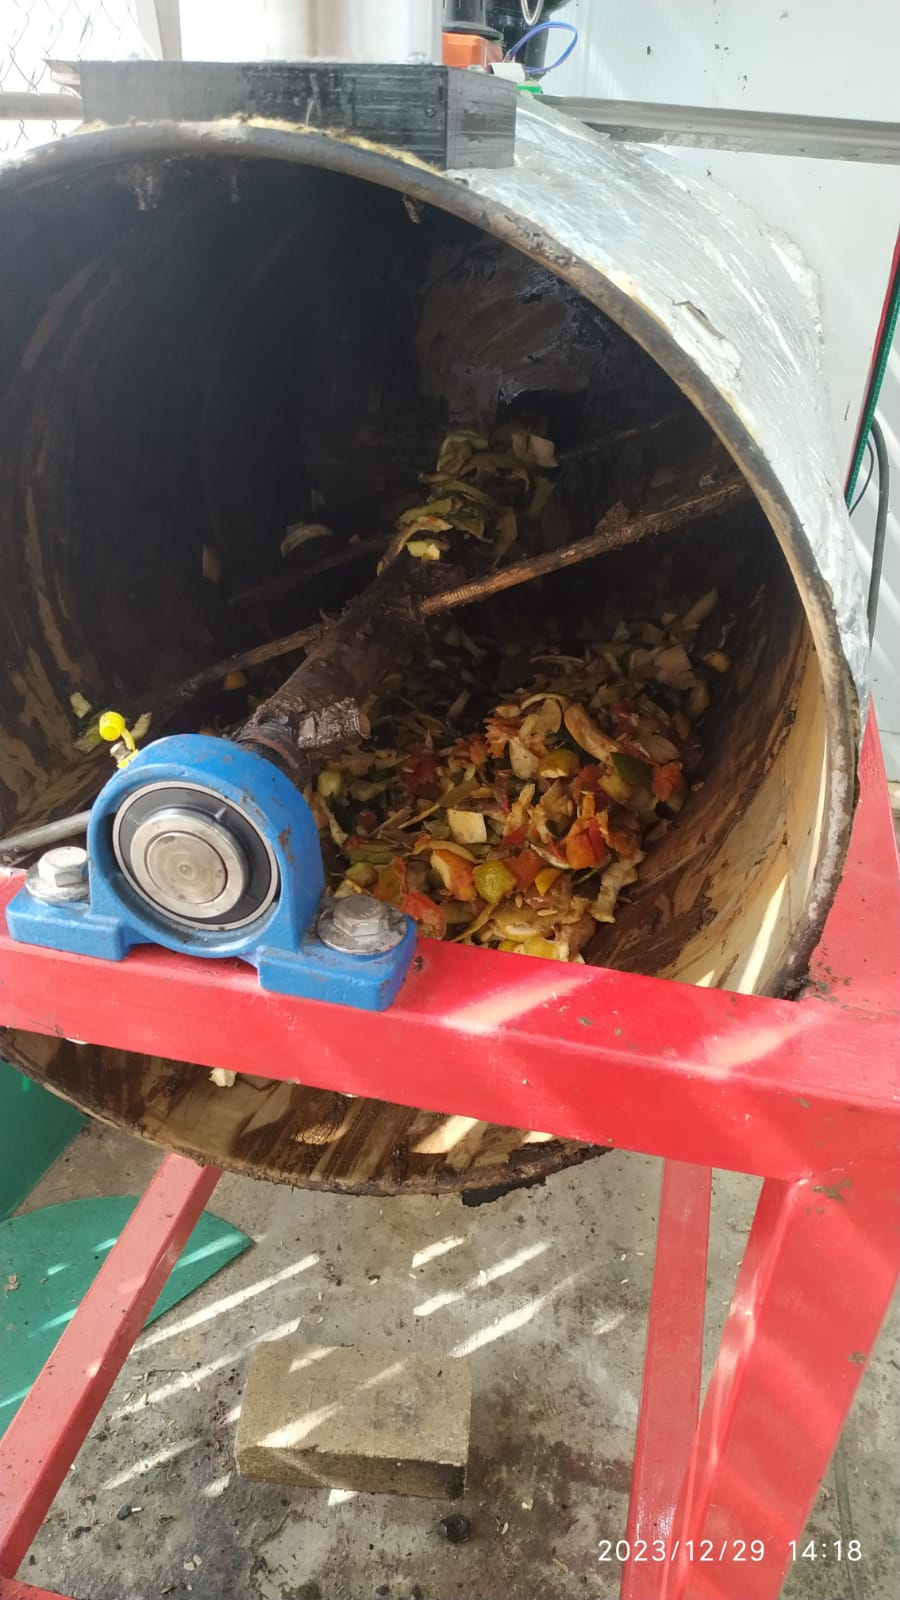
\includegraphics[scale=0.15]{images/Pruebas/Pruebas_compost/carga6.jpeg}
    \caption{Sexta prueba carga}
    \label{fg:carga6}
\end{figure}

Desafortunadamente en el lugar que se encuentra el dispositivo estuvo presentando cortes de energía eléctrica, se estima que el ciclo se detuvo a las 40 horas del proceso obteniéndose el siguiente resultado:

\begin{figure}[h]
    \centering
    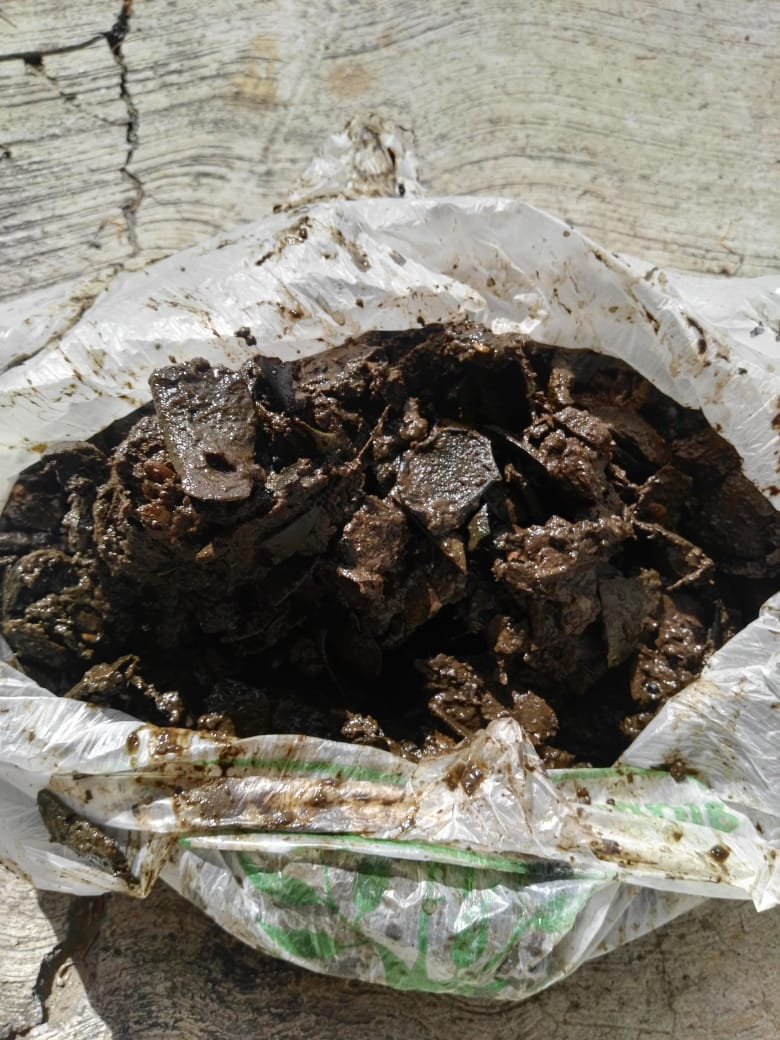
\includegraphics[scale=0.15]{images/Pruebas/Pruebas_compost/descarga6.jpeg}
    \caption{Sexta prueba descarga}
    \label{fg:descarga6}
\end{figure}

Como se puede observar, se trata de una mezcla heterogénea en donde claramente se distingue la mayoría de los residuos, añadiendo que la cantidad de agua contenida resulta exagerada. Esto, a consecuencia de la interrupción del proceso, presenta un olor desagradable, similar al de un alimento en descomposición, debido también al tiempo que pasó dentro del contenedor. Y, aunque este intento se considera fallido, se ha decidido registrarlo, puesto que brinda cierta retroalimentación sobre posibles mejoras a futuro. Por otro lado, es importante señalar que las muestras exitosas fueron consistentes, ya que la cantidad de compost obtenida es cerca del 43\% del total ingresado.

\clearpage

\textbf{\textit{Pruebas de pH}}

Para verificar la calidad del compost obtenido, se realizaron pruebas de pH para verificar la estabilidad de la mezcla. Se muestran las imágenes de las pruebas realizadas y los resultados obtenidos en la Tabla \ref{tab:pruebas_compostaje}. Es importante señalar que, aunque se llevaron a cabo seis pruebas de compostaje, solo se realizaron mediciones de pH y registro fotográfico para las primeras cinco muestras. La sexta prueba fue interrumpida y no cuenta con imágenes ni medición de pH, por lo que se incluye únicamente en la tabla resumen como caso fallido.

El proceso completo de medición se documenta en las Figuras \ref{fg:muestra1_proceso} a \ref{fg:muestra5_proceso}, donde cada figura ilustra tres etapas clave: el pesaje de la muestra, la comparativa colorimétrica y la lectura con el pHmetro. Estas imágenes permiten corroborar visualmente las condiciones de cada muestra y respaldan los resultados numéricos presentados en la Tabla \ref{tab:pruebas_compostaje}.

La primera muestra, correspondiente a la prueba 1, se caracterizó por una mezcla homogénea de color marrón intenso y un olor afrutado, similar al ponche de frutas. Sin embargo, presentó un contenido de humedad excesivo que no pudo corregirse ni siquiera tras 24 horas adicionales de ciclo, lo que se refleja en un pH final de 8.83.

\begin{figure}[htbp]
    \centering
    \begin{subfigure}[b]{0.28\textwidth}
        \centering
        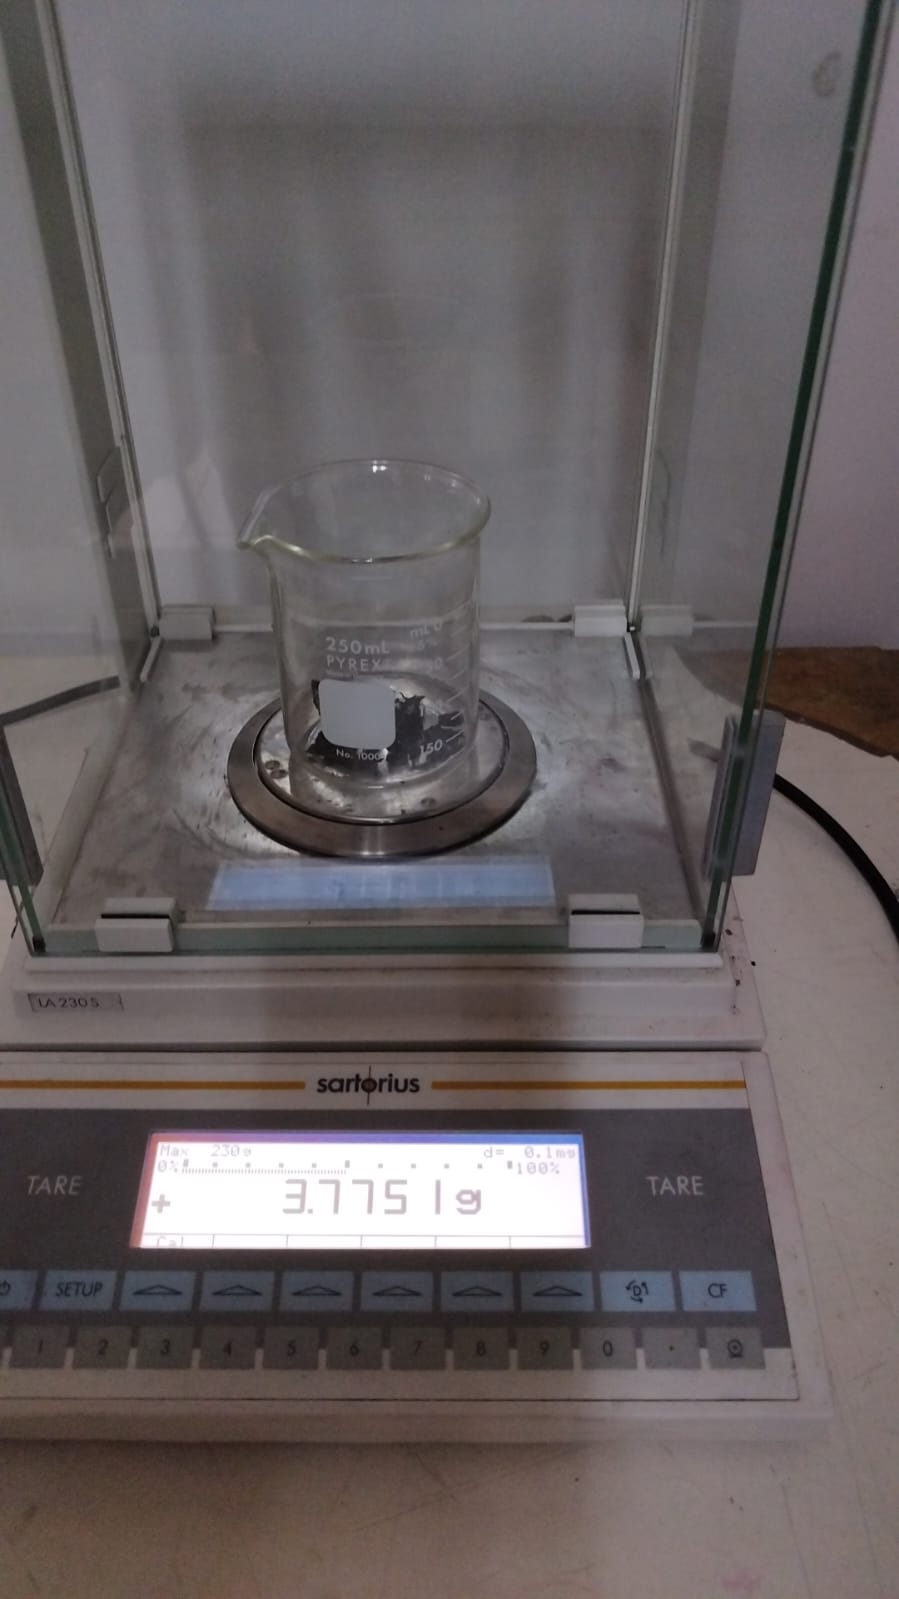
\includegraphics[width=\textwidth]{images/Pruebas/Resultados/muestra_1.jpeg}
        \caption{Pesaje}
        \label{fg:m1_pesaje}
    \end{subfigure}
    \hfill
    \begin{subfigure}[b]{0.32\textwidth}
        \centering
        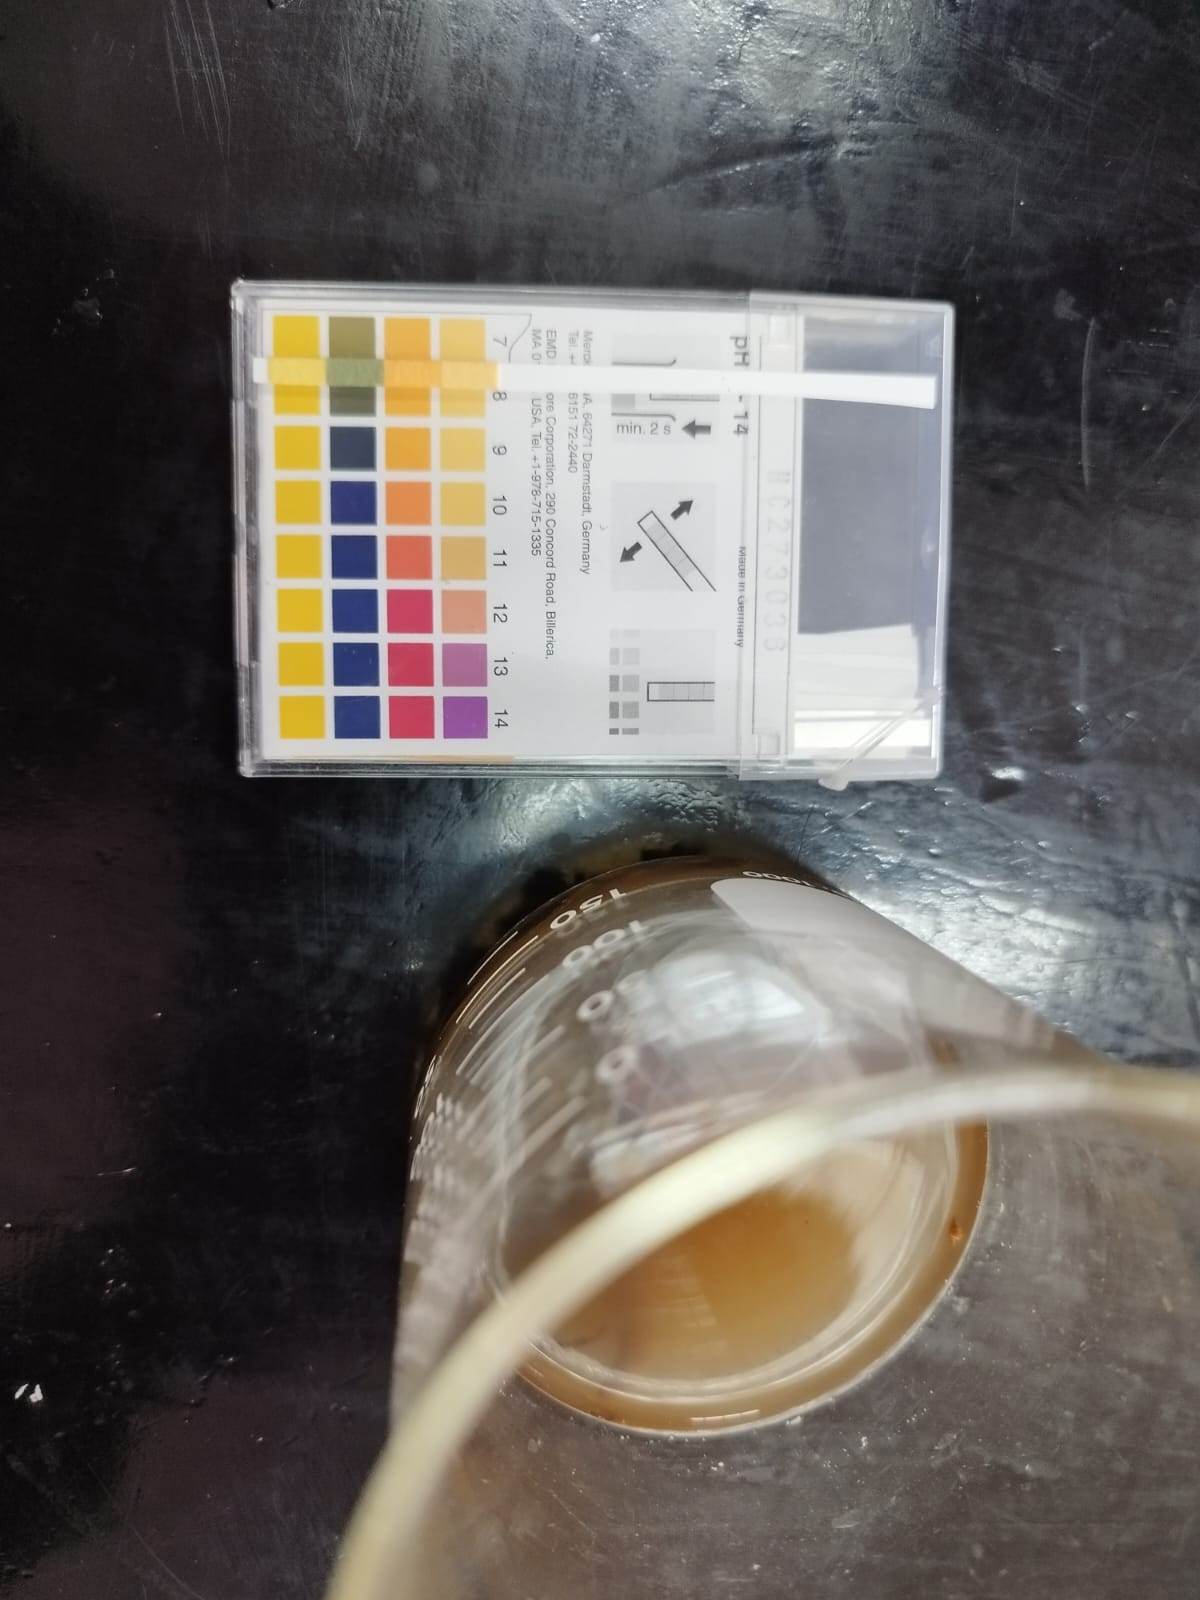
\includegraphics[width=\textwidth]{images/Pruebas/Resultados/muestra_1_colorimetria.jpeg}
        \caption{Comparativa colorimétrica}
        \label{fg:m1_color}
    \end{subfigure}
    \hfill
    \begin{subfigure}[b]{0.32\textwidth}
        \centering
        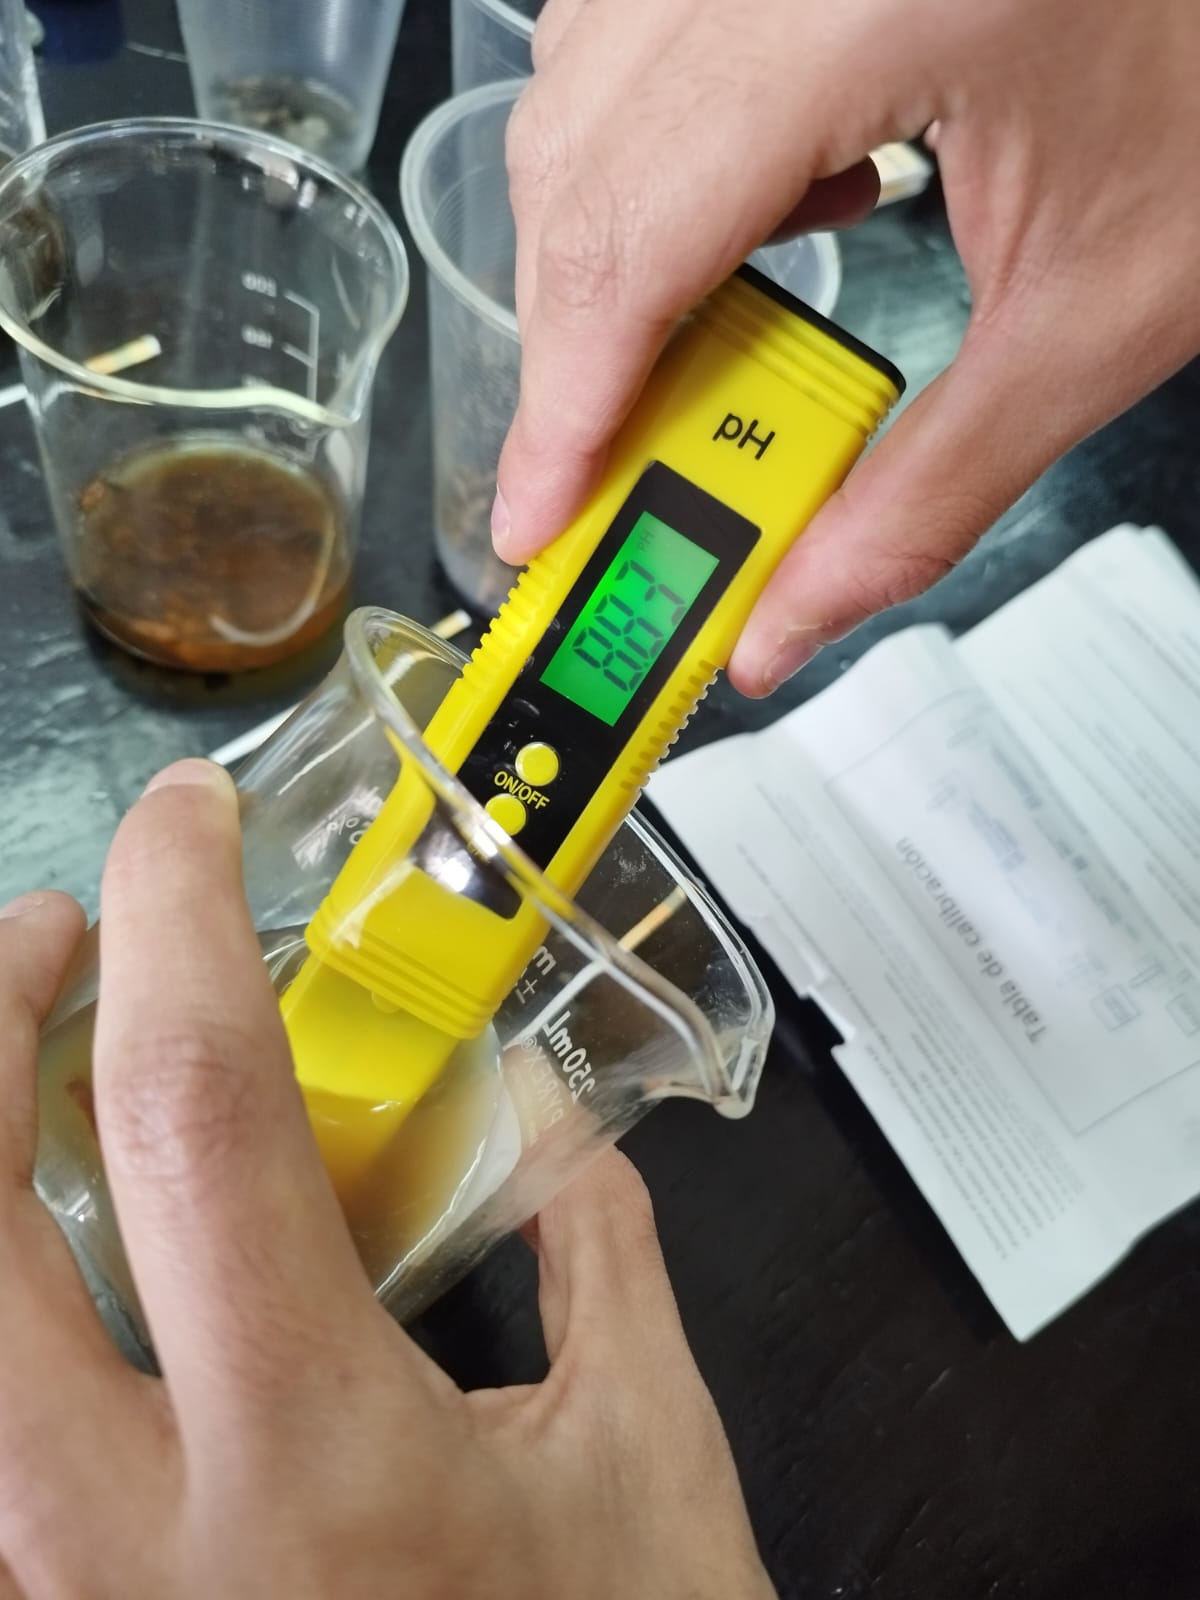
\includegraphics[width=\textwidth]{images/Pruebas/Resultados/muestra_1_phmetro.jpeg}
        \caption{Lectura de pHmetro}
        \label{fg:m1_ph}
    \end{subfigure}
    \caption{Proceso de medición de pH — Muestra 1}
    \label{fg:muestra1_proceso}
\end{figure}

En Figura \ref{fg:muestra1_proceso} se presenta la muestra durante las etapas de pesaje, comparación colorimétrica y medición con el pHmetro. 

La segunda muestra, asociada a la prueba 2, mantuvo la misma problemática de humedad excesiva que la primera, sin que se lograra reducir el agua durante el proceso. Aunque no se reportó la cantidad de compost obtenido, el pH final fue de 7.96, ligeramente superior al de la muestra anterior.

\begin{figure}[htbp]
    \centering
    \begin{subfigure}[b]{0.28\textwidth}
        \centering
        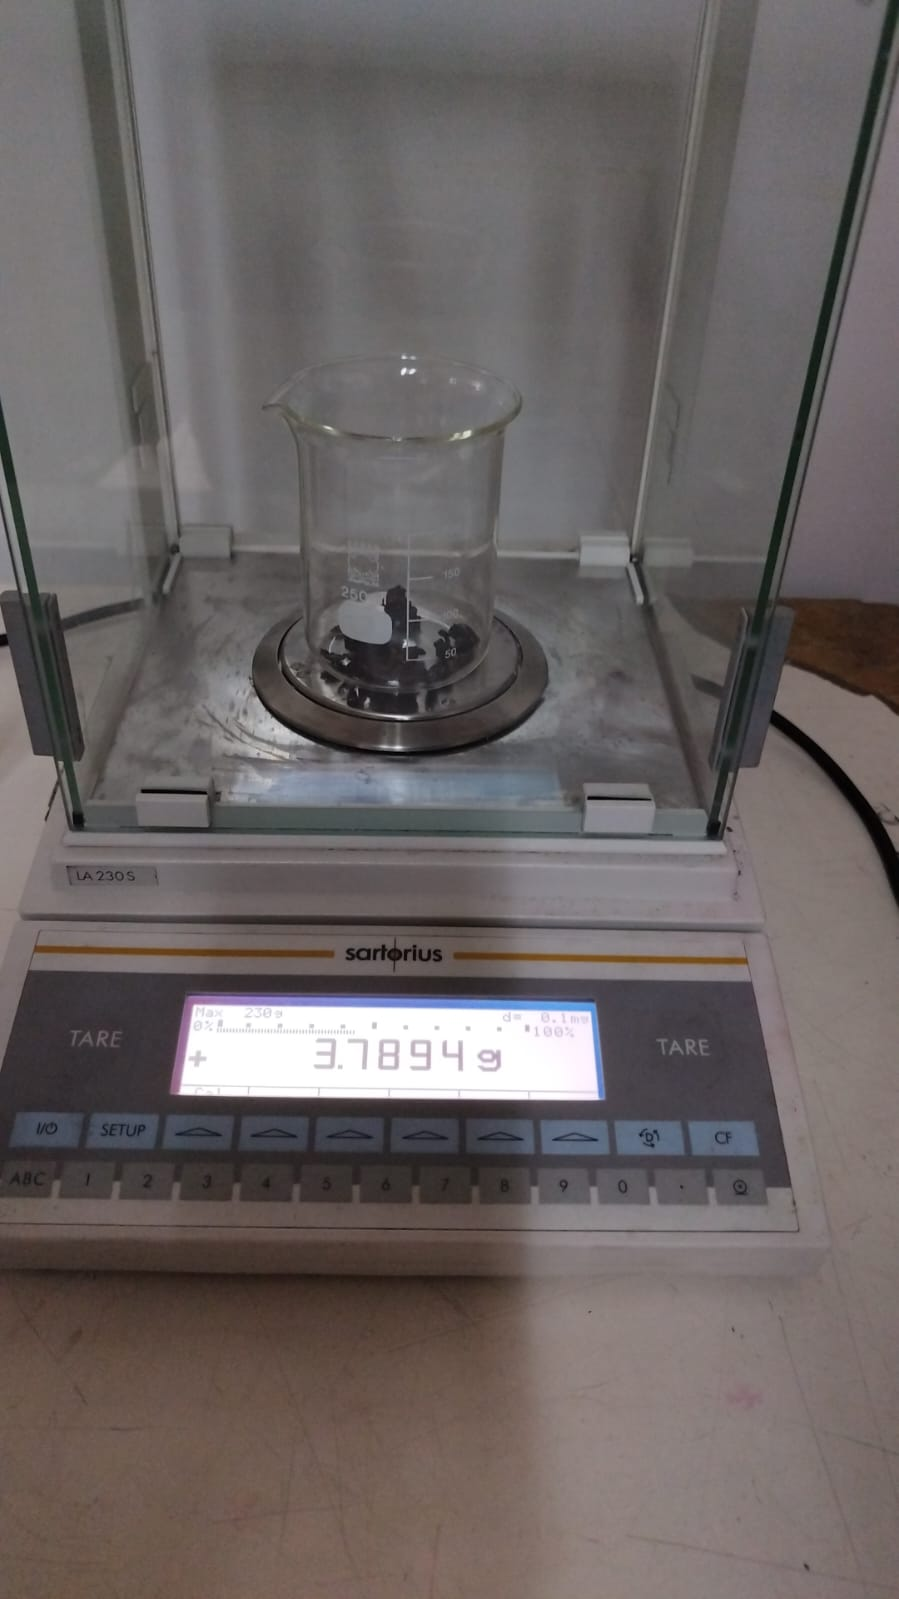
\includegraphics[width=\textwidth]{images/Pruebas/Resultados/muestra_2.jpeg}
        \caption{Pesaje}
        \label{fg:m2_pesaje}
    \end{subfigure}
    \hfill
    \begin{subfigure}[b]{0.32\textwidth}
        \centering
        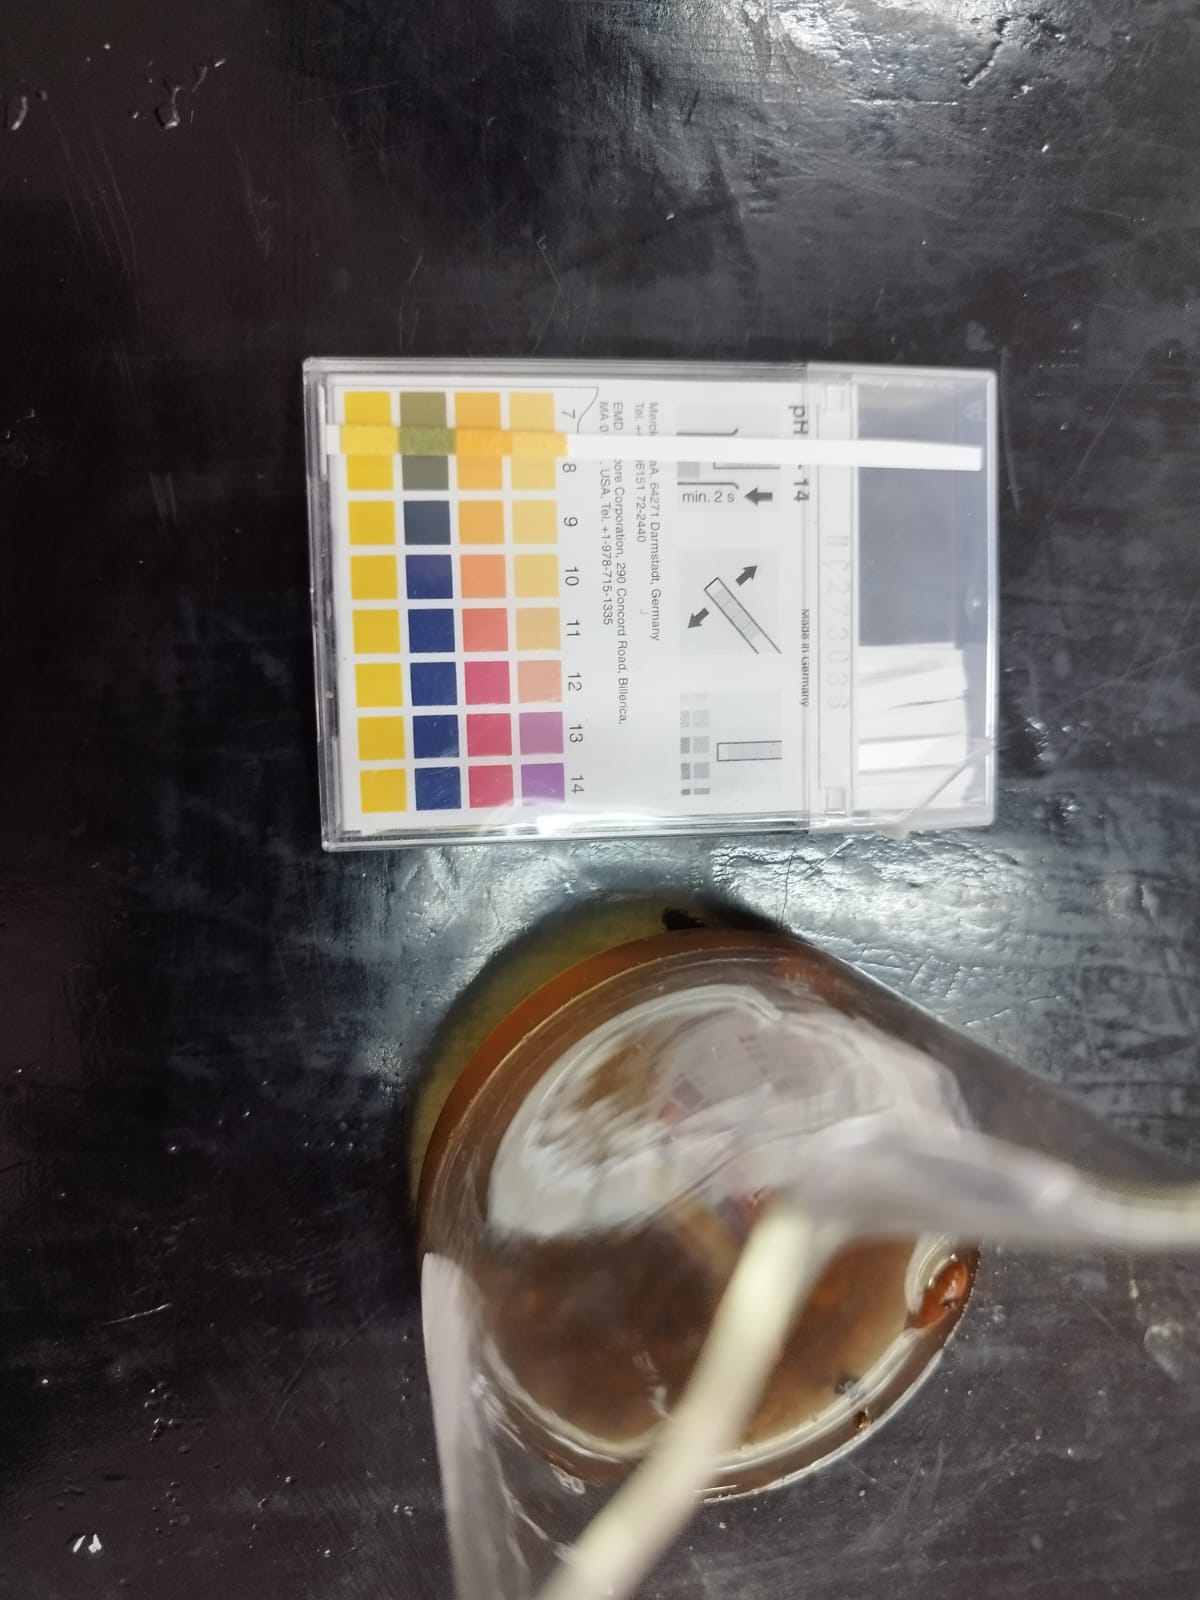
\includegraphics[width=\textwidth]{images/Pruebas/Resultados/muestra_2_colorimetria.jpeg}
        \caption{Comparativa colorimétrica}
        \label{fg:m2_color}
    \end{subfigure}
    \hfill
    \begin{subfigure}[b]{0.32\textwidth}
        \centering
        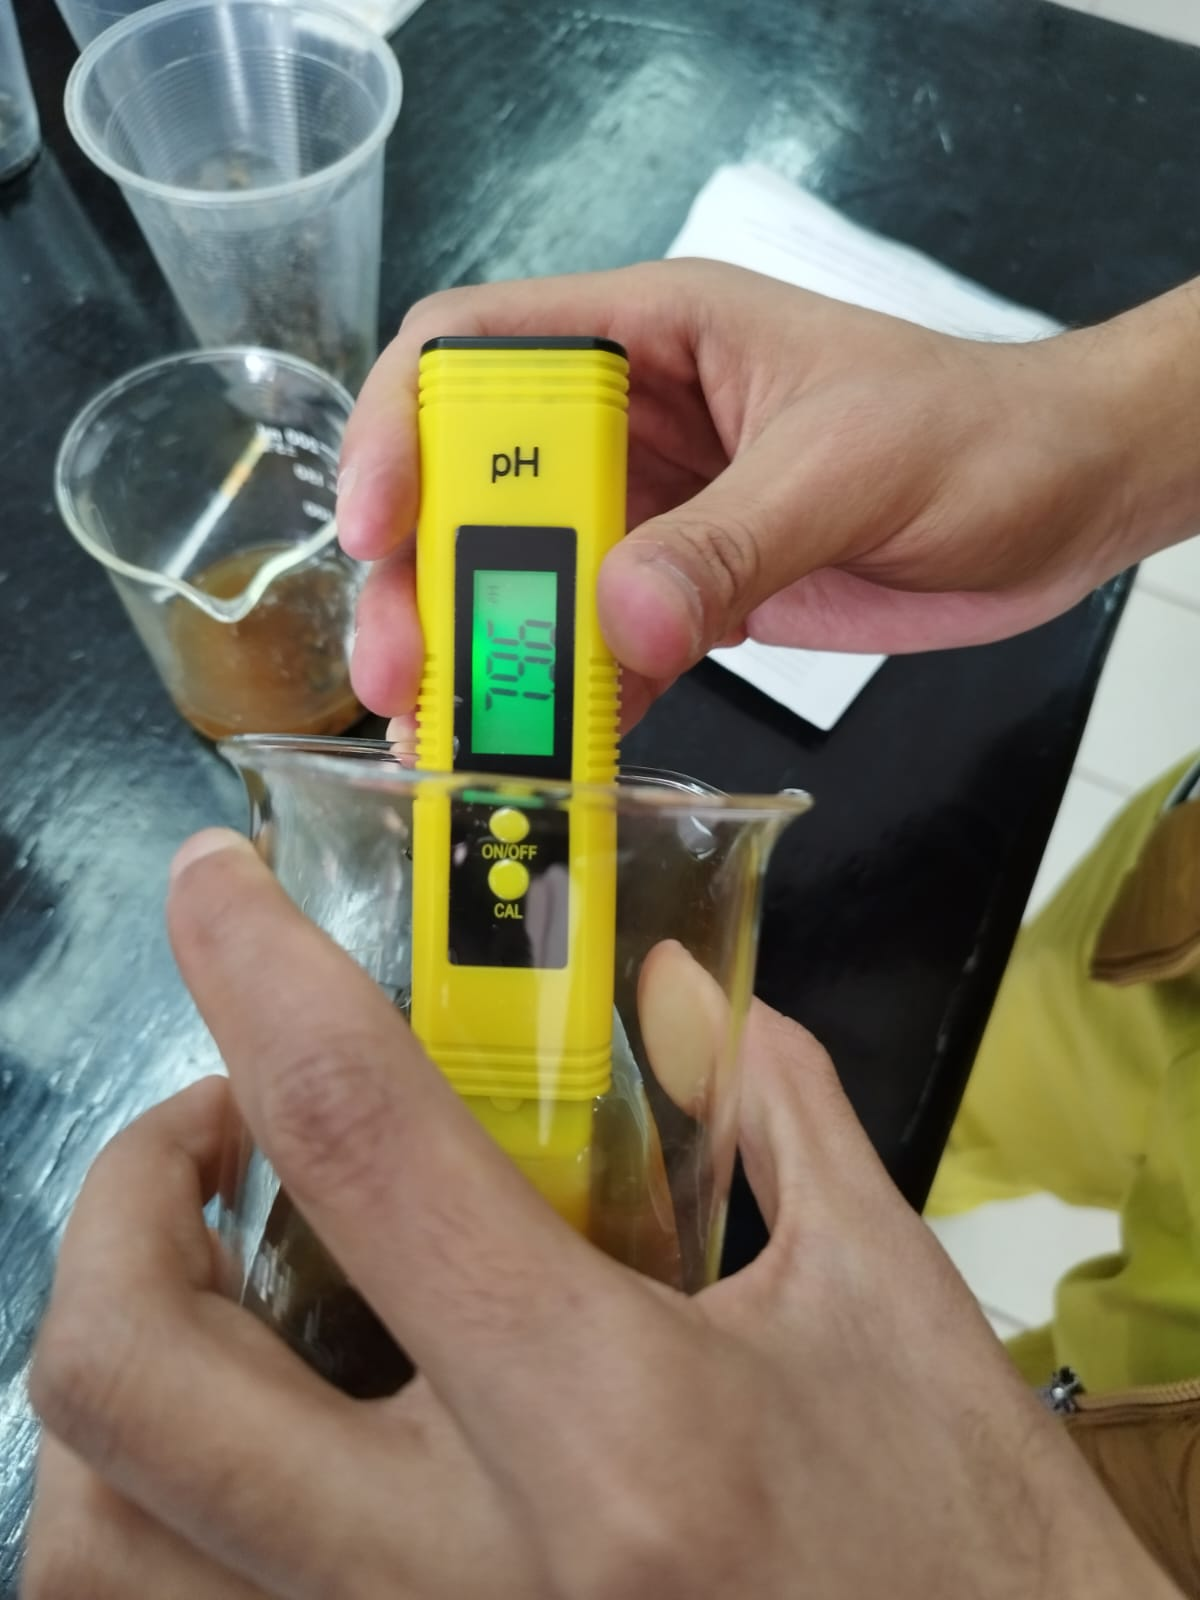
\includegraphics[width=\textwidth]{images/Pruebas/Resultados/muestra_2_phmetro.jpeg}
        \caption{Lectura de pHmetro}
        \label{fg:m2_ph}
    \end{subfigure}
    \caption{Proceso de medición de pH — Muestra 2}
    \label{fg:muestra2_proceso}
\end{figure}

Las imágenes de la Figura \ref{fg:muestra2_proceso} evidencian una consistencia aún muy húmeda y una coloración similar a la de la muestra 1. 

En contraste, la tercera muestra (prueba 3) presentó las mejores condiciones de procesamiento: los residuos fueron totalmente triturados hasta partículas de aproximadamente 3 mm, lo que favoreció un compost de aspecto similar a la tierra, con partícula fina, color café oscuro, olor a durazno y humedad mínima. Esta muestra se deshacía al soltarla y alcanzó un pH de 7.62, el más cercano a la neutralidad entre las pruebas exitosas.

\begin{figure}[H]
    \centering
    \begin{subfigure}[b]{0.30\textwidth}
        \centering
        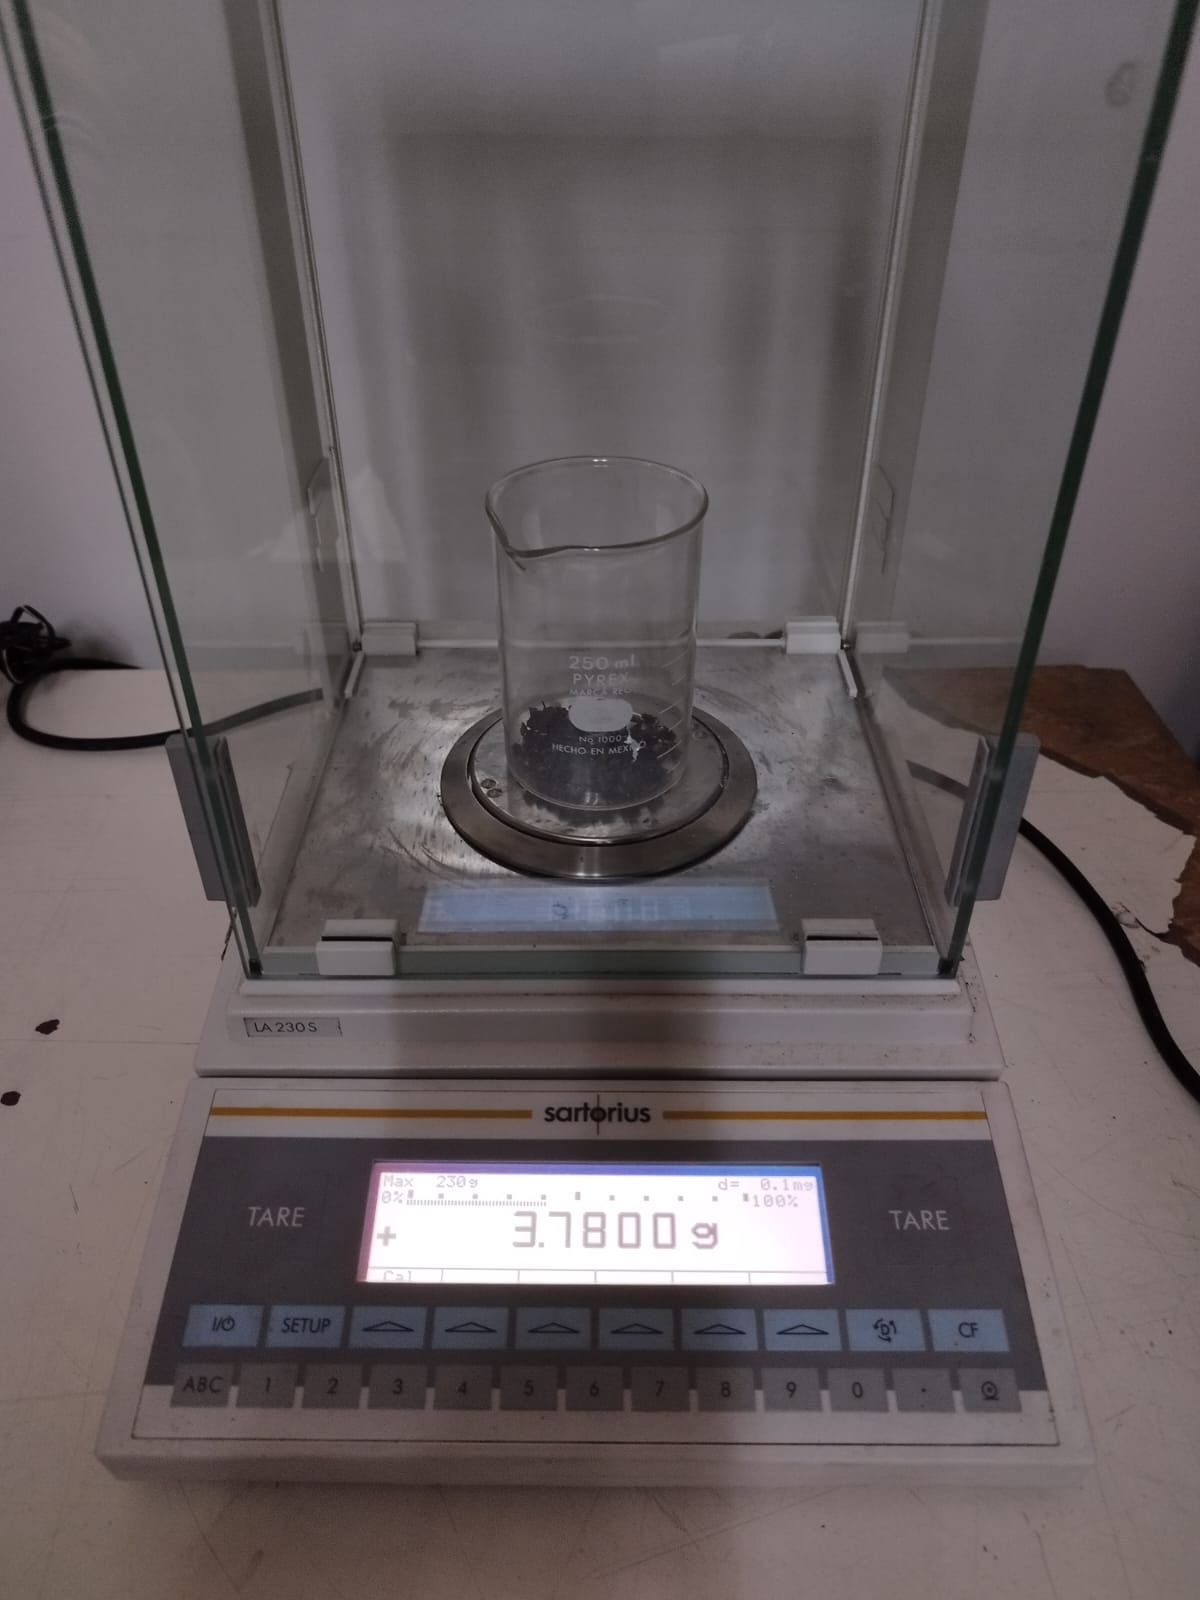
\includegraphics[width=\textwidth]{images/Pruebas/Resultados/muestra_3.jpeg}
        \caption{Pesaje}
        \label{fg:m3_pesaje}
    \end{subfigure}
    \hfill
    \begin{subfigure}[b]{0.32\textwidth}
        \centering
        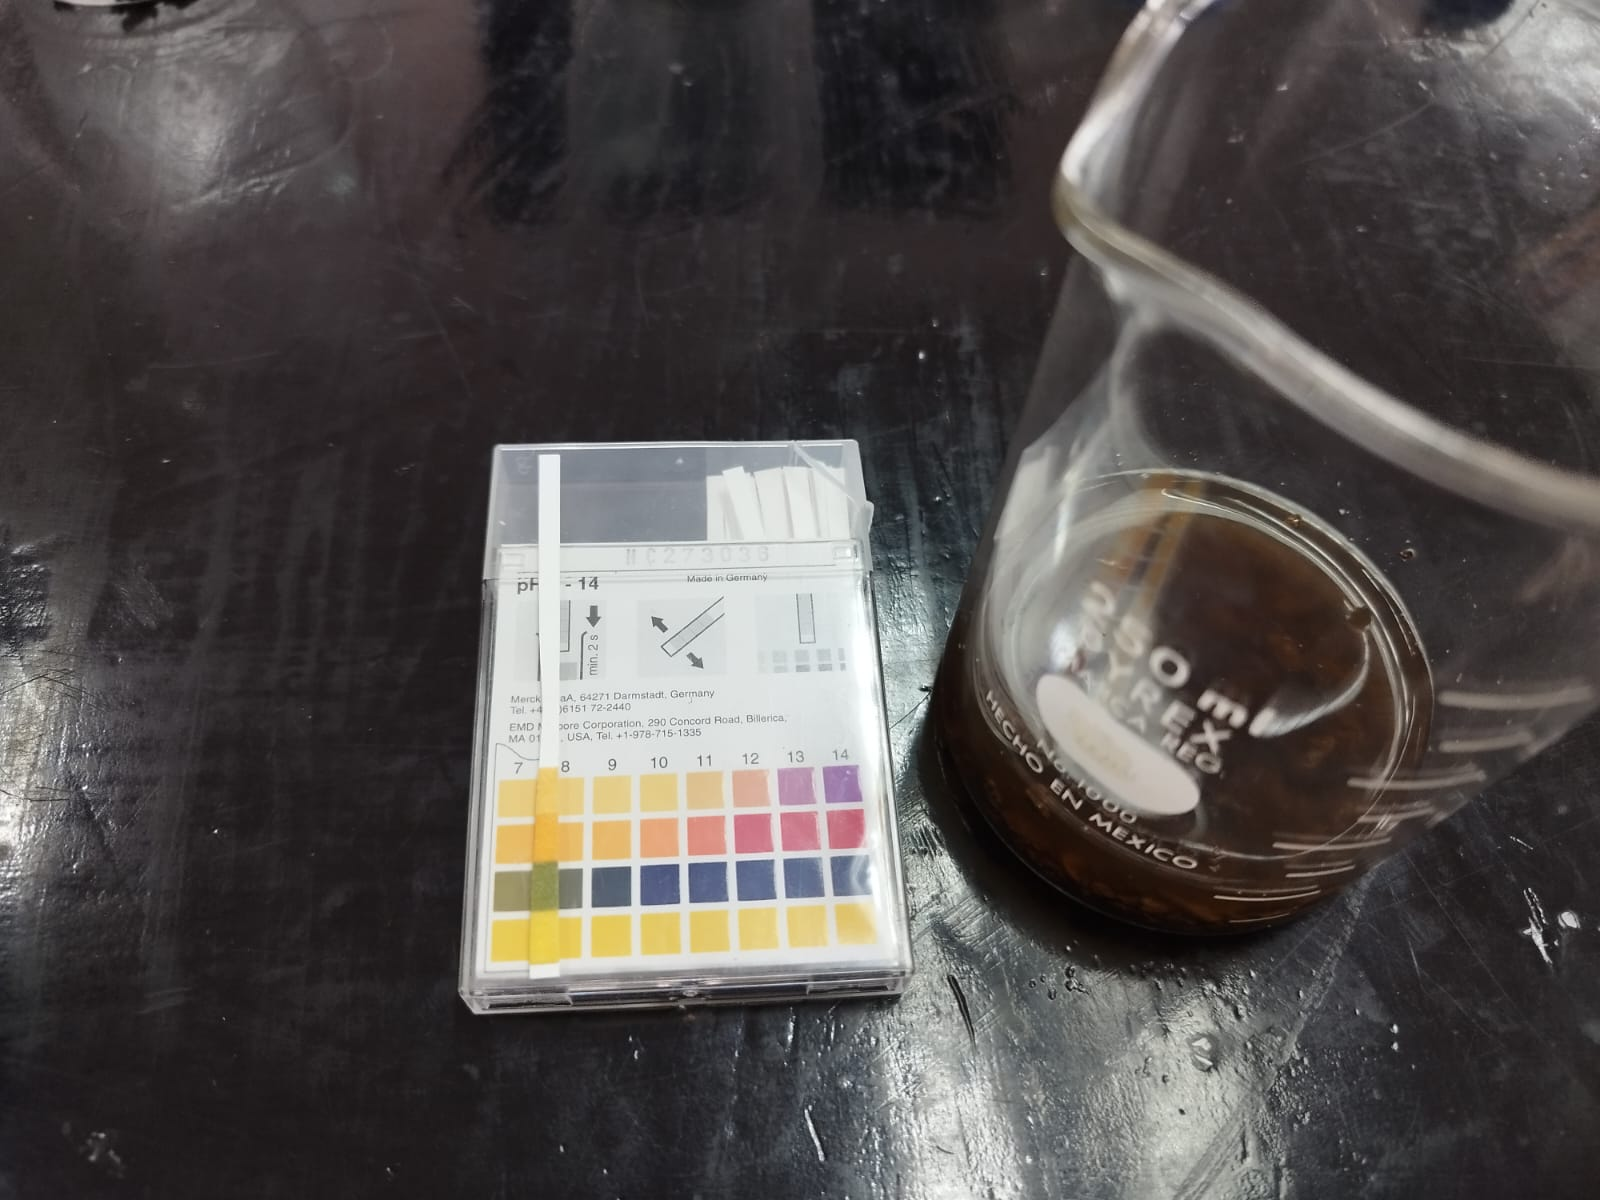
\includegraphics[width=\textwidth]{images/Pruebas/Resultados/muestra_3_colorimetria.jpeg}
        \caption{Comparativa colorimétrica}
        \label{fg:m3_color}
    \end{subfigure}
    \hfill
    \begin{subfigure}[b]{0.30\textwidth}
        \centering
        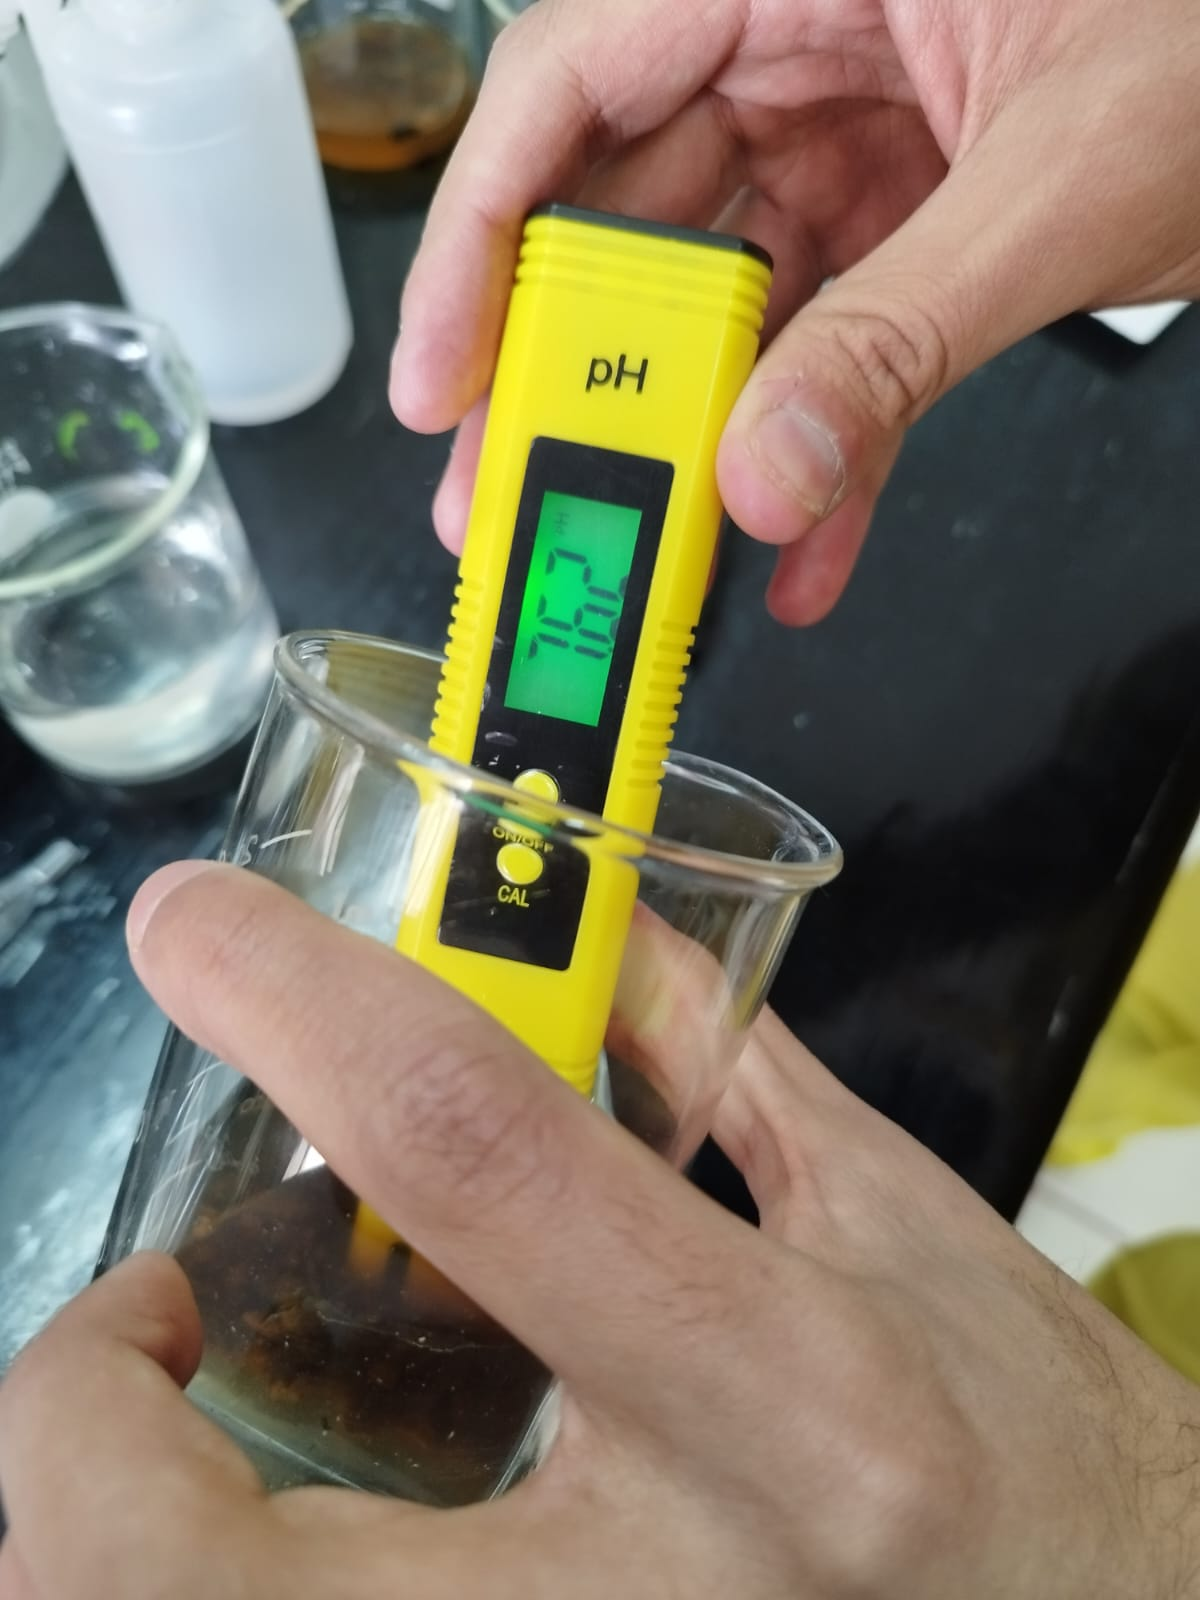
\includegraphics[width=\textwidth]{images/Pruebas/Resultados/muestra_3_phmetro.jpeg}
        \caption{Lectura de pHmetro}
        \label{fg:m3_ph}
    \end{subfigure}
    \caption{Proceso de medición de pH — Muestra 3}
    \label{fg:muestra3_proceso}
\end{figure}

La Figura \ref{fg:muestra3_proceso} documenta estas características visuales.

La cuarta muestra (prueba 4) correspondió a una preparación mixta: la mitad de los residuos fue triturada y la otra mitad picada. El compost resultante fue homogéneo, con humedad moderada y un olor frutal agradable, alcanzando un pH de 5.33.

\begin{figure}[H]
    \centering
    \begin{subfigure}[b]{0.32\textwidth}
        \centering
        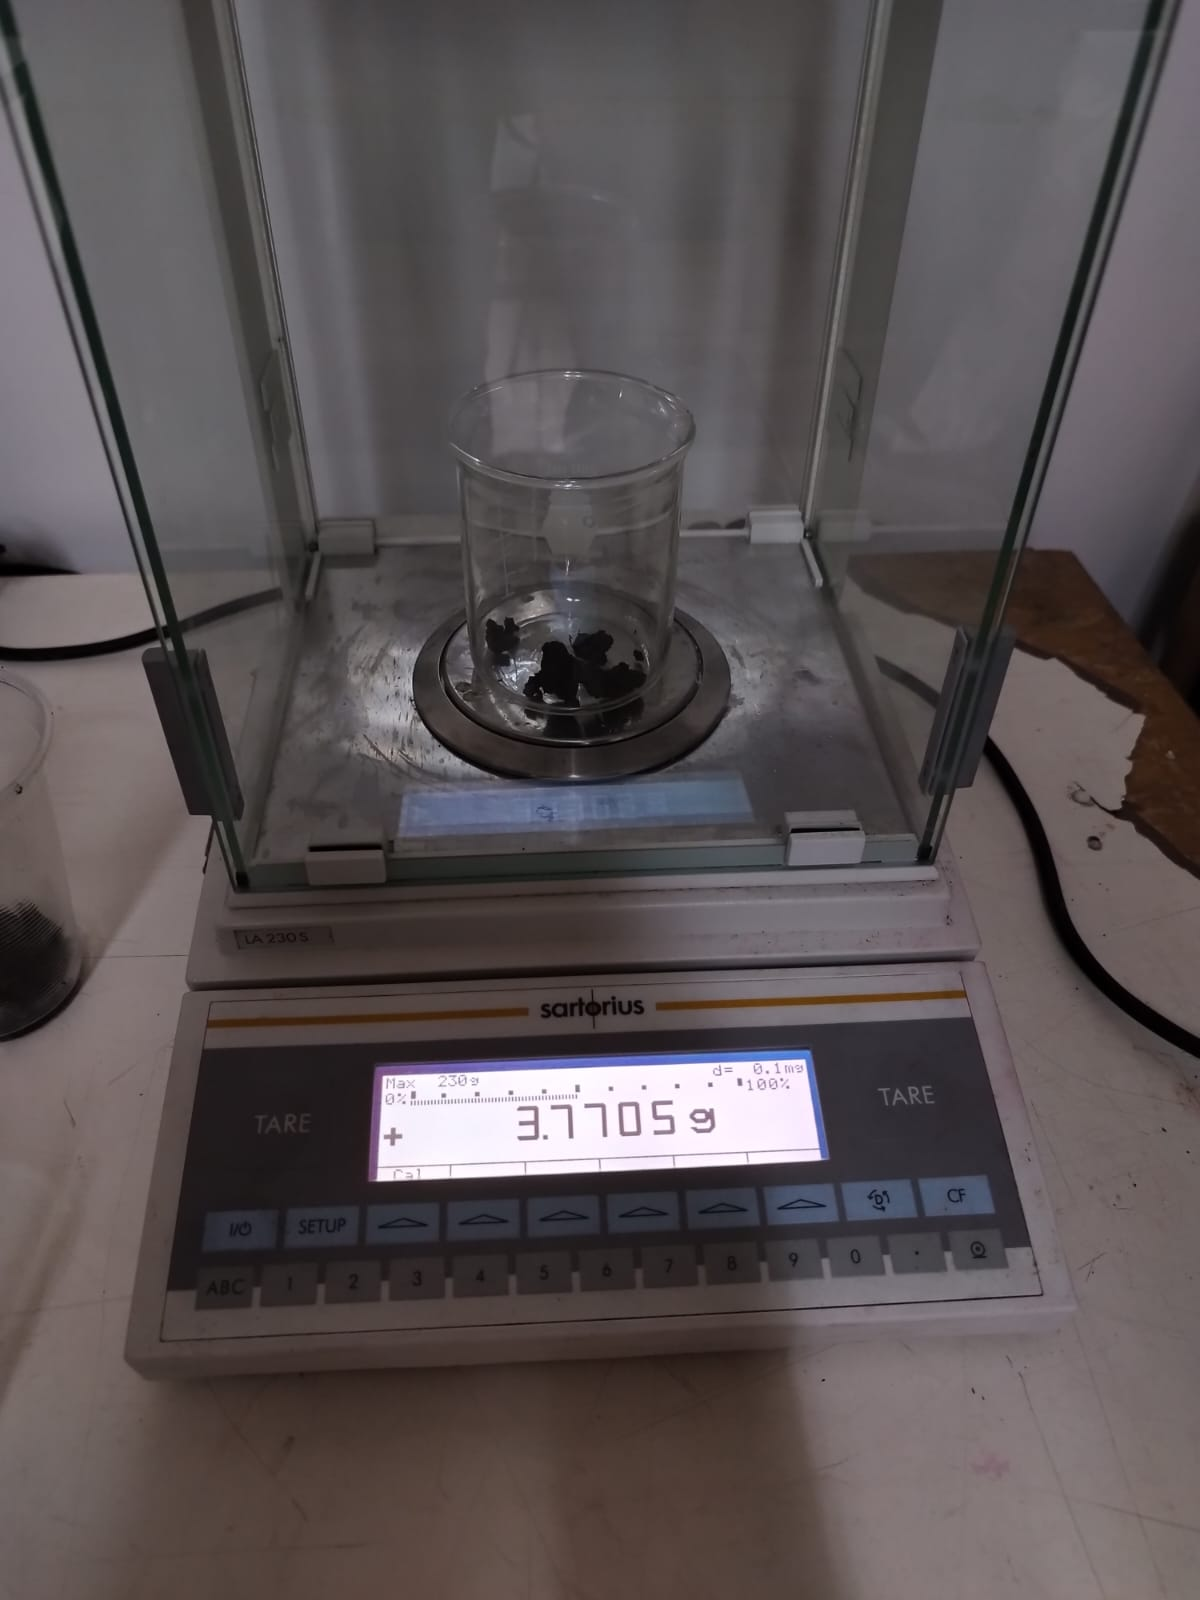
\includegraphics[width=\textwidth]{images/Pruebas/Resultados/muestra_4.jpeg}
        \caption{Pesaje}
        \label{fg:m4_pesaje}
    \end{subfigure}
    \hfill
    \begin{subfigure}[b]{0.32\textwidth}
        \centering
        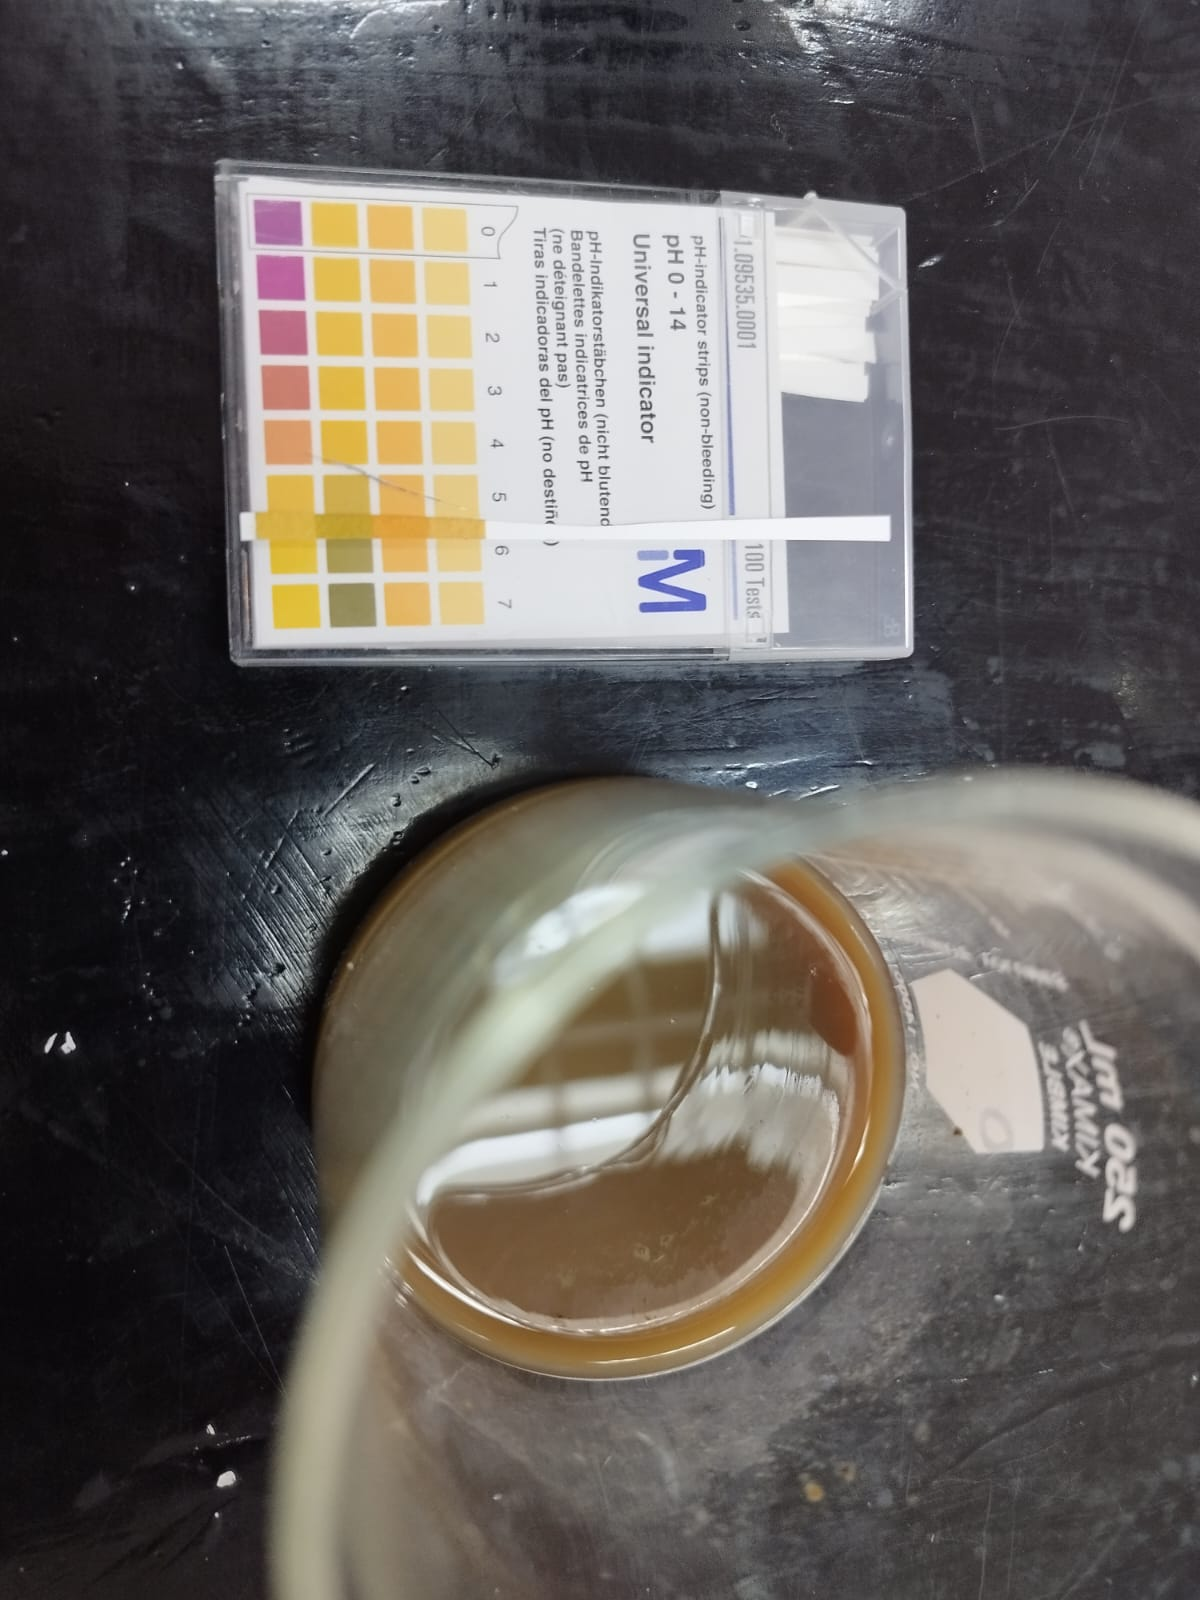
\includegraphics[width=\textwidth]{images/Pruebas/Resultados/muestra_4_colorimetria.jpeg}
        \caption{Comparativa colorimétrica}
        \label{fg:m4_color}
    \end{subfigure}
    \hfill
    \begin{subfigure}[b]{0.32\textwidth}
        \centering
        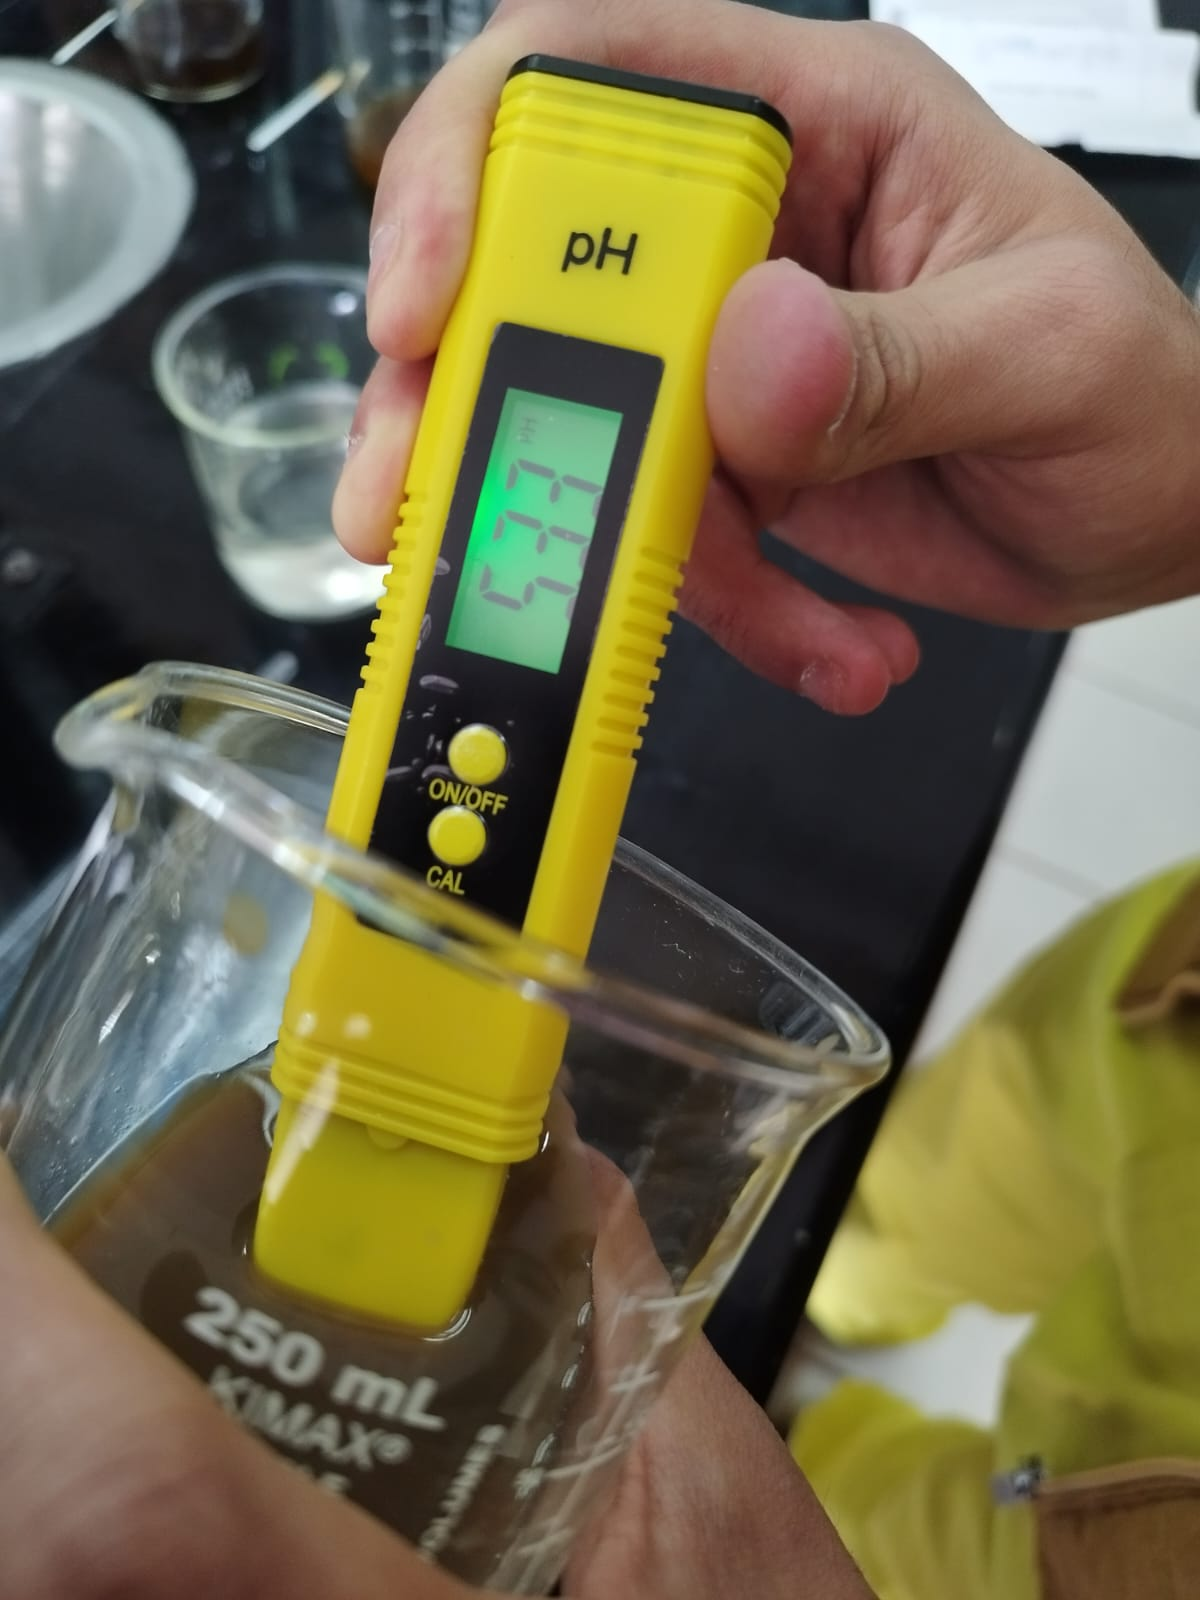
\includegraphics[width=\textwidth]{images/Pruebas/Resultados/muestra_4_phmetro.jpeg}
        \caption{Lectura de pHmetro}
        \label{fg:m4_ph}
    \end{subfigure}
    \caption{Proceso de medición de pH — Muestra 4}
    \label{fg:muestra4_proceso}
\end{figure}

La Figura \ref{fg:muestra4_proceso} muestra el pesaje, la comparativa colorimétrica y la lectura de pH para esta muestra. 

Finalmente, la quinta muestra (prueba 5) se obtuvo a partir de residuos frescos y muy húmedos que solo fueron picados. El compost presentó una consistencia pastosa, descrita como similar a mole o lodo, con color café oscuro y olor agradable, pero con un exceso de agua evidente. Su pH final fue de 7.15, y el rendimiento alcanzó el 48.4\,\%, el más alto entre las pruebas exitosas.

\begin{figure}[H]
    \centering
    \begin{subfigure}[b]{0.32\textwidth}
        \centering
        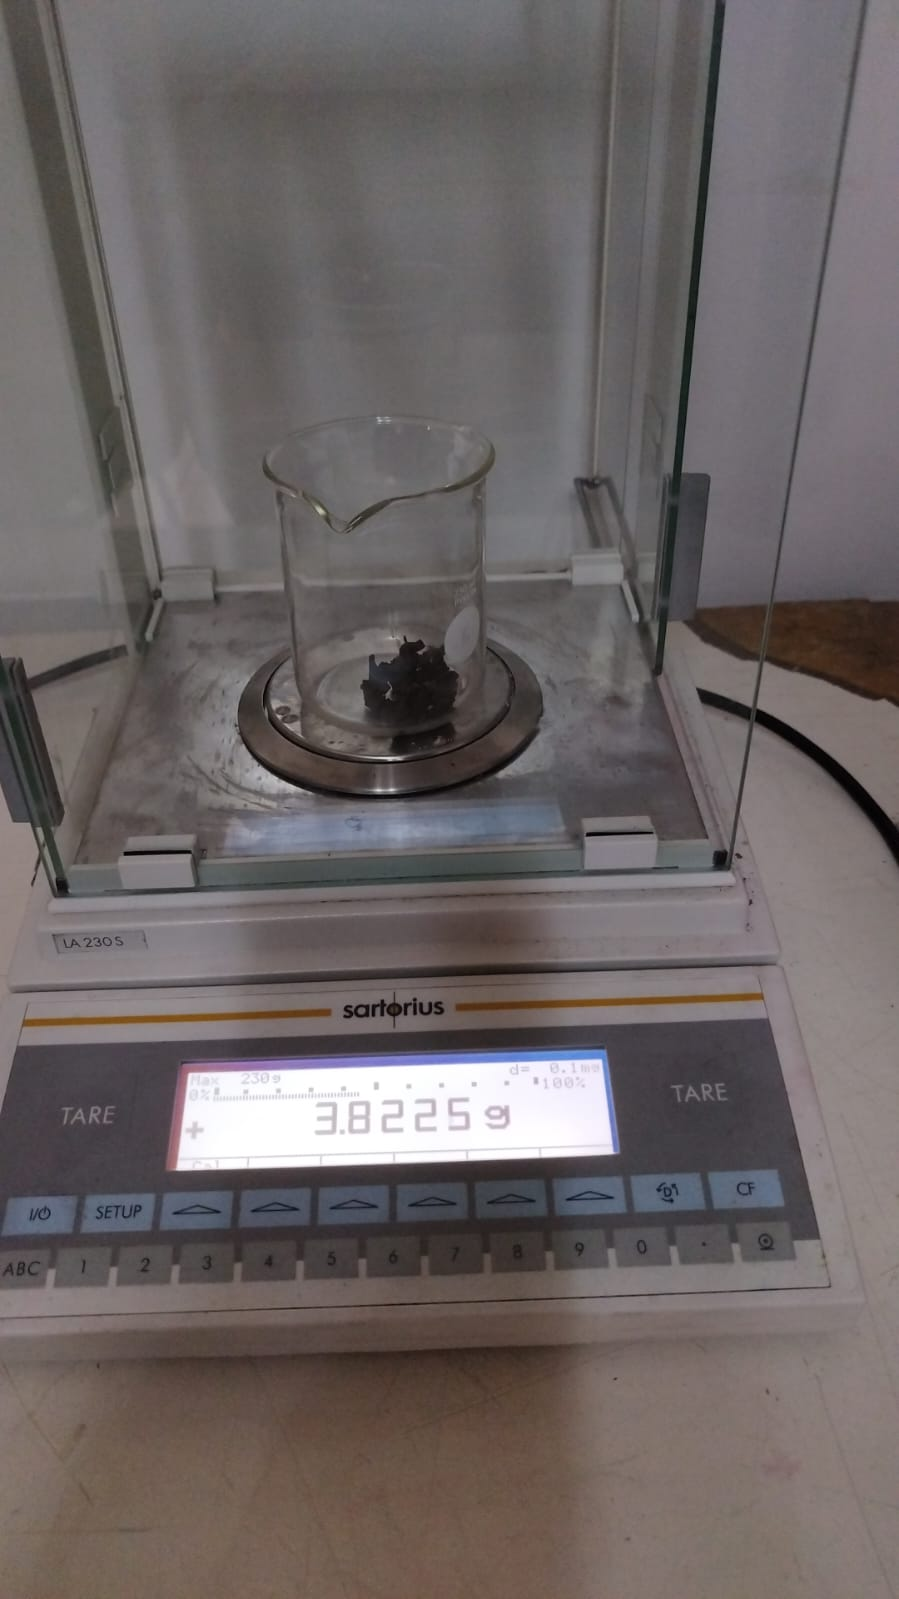
\includegraphics[width=\textwidth]{images/Pruebas/Resultados/muestra_5.jpeg}
        \caption{Pesaje}
        \label{fg:m5_pesaje}
    \end{subfigure}
    \hfill
    \begin{subfigure}[b]{0.32\textwidth}
        \centering
        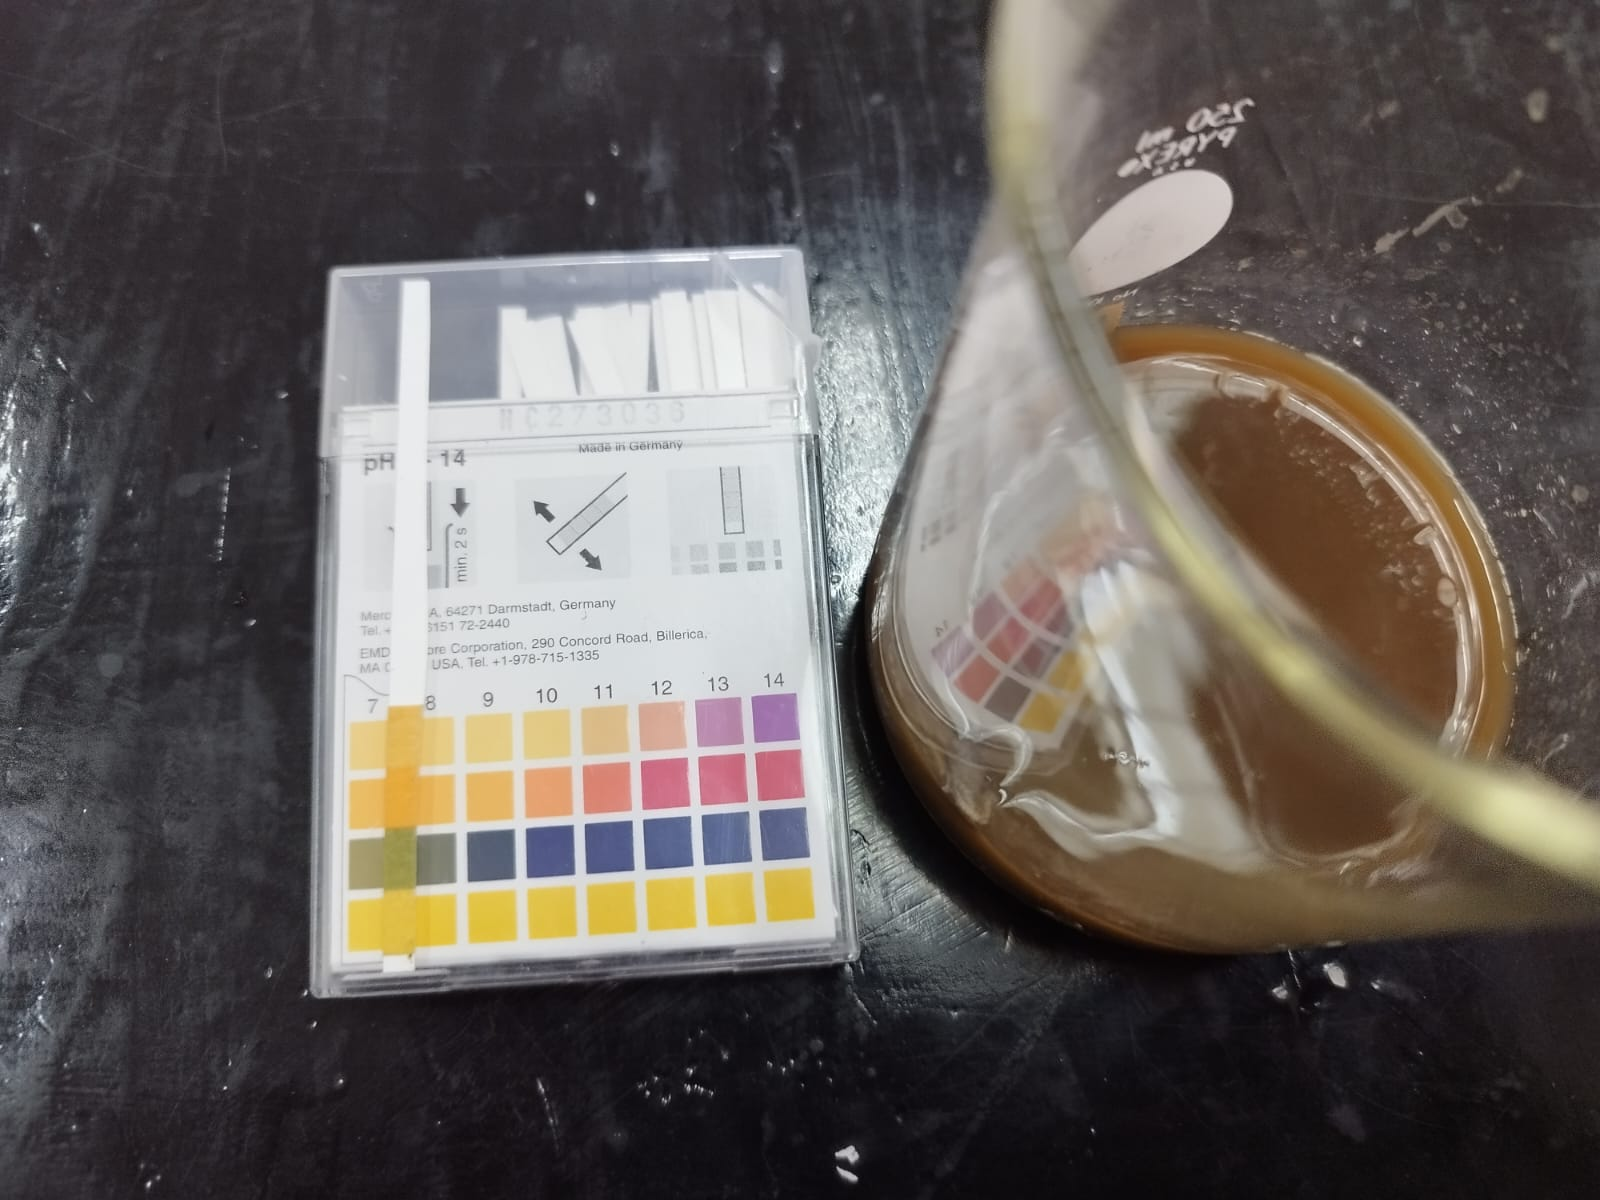
\includegraphics[width=\textwidth]{images/Pruebas/Resultados/muestra_5_colorimetria.jpeg}
        \caption{Comparativa colorimétrica}
        \label{fg:m5_color}
    \end{subfigure}
    \hfill
    \begin{subfigure}[b]{0.32\textwidth}
        \centering
        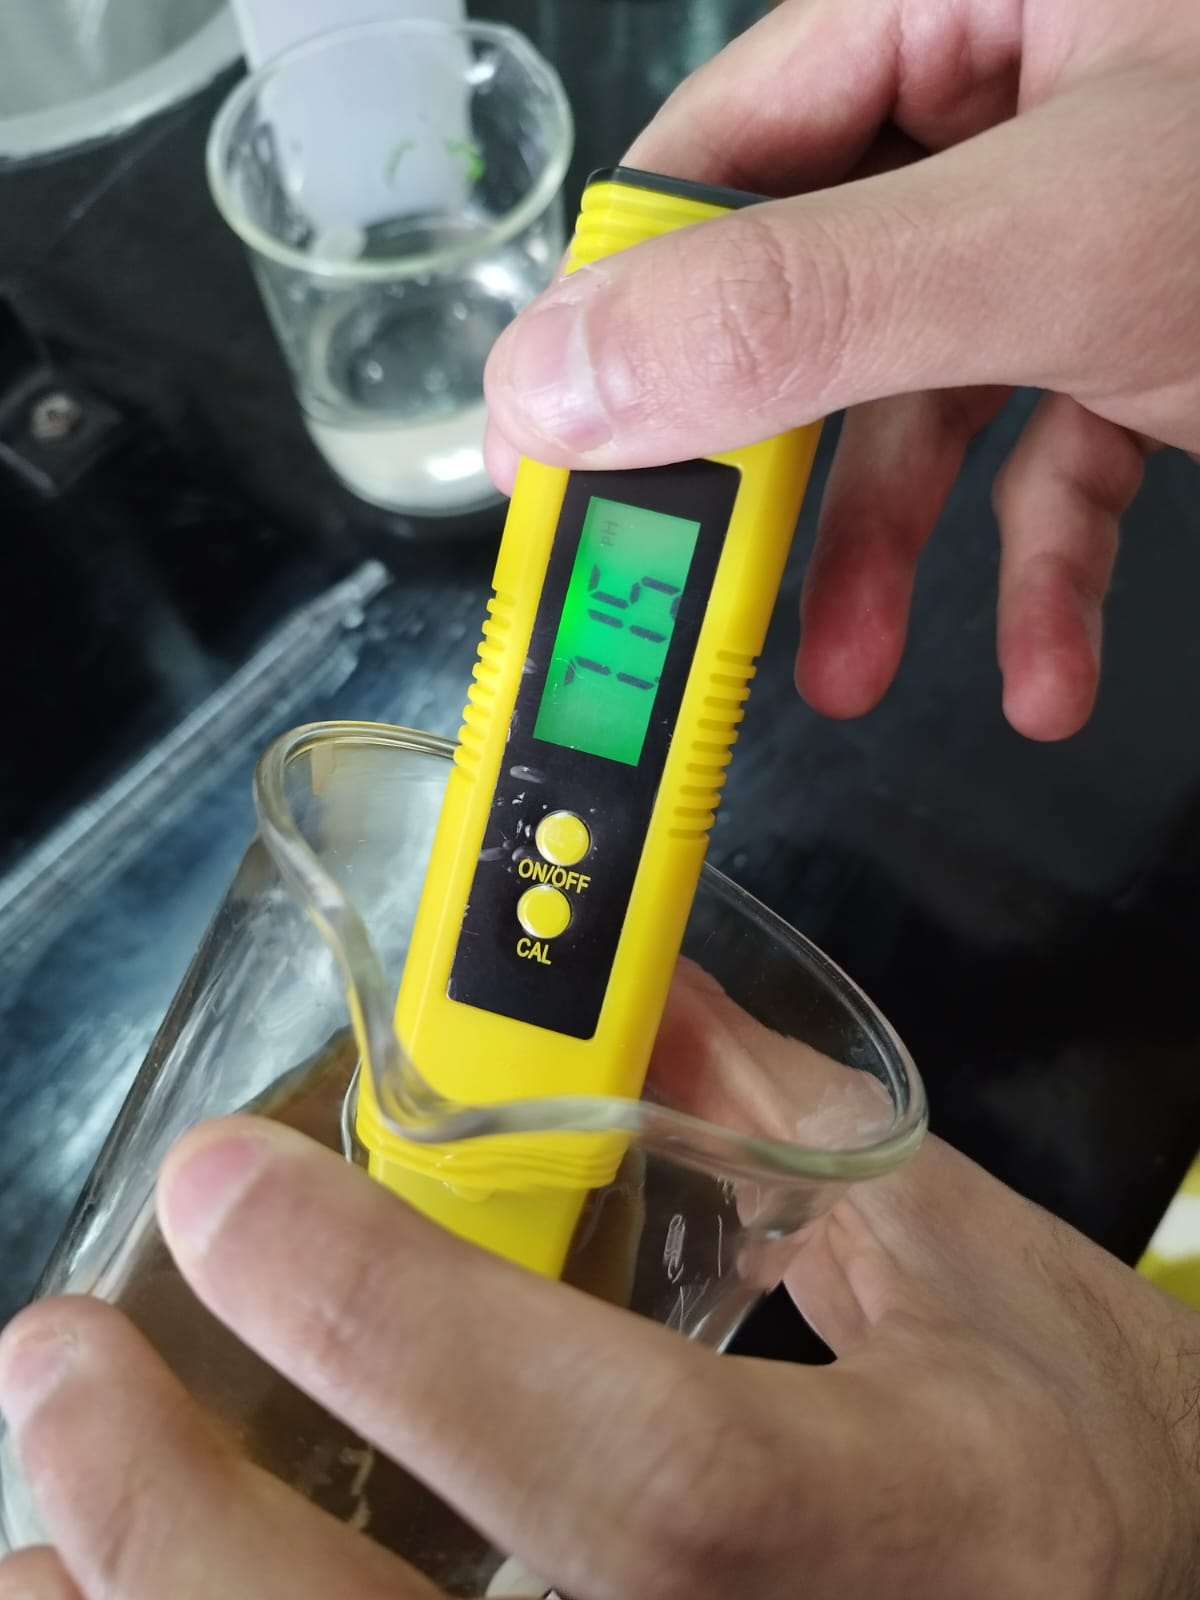
\includegraphics[width=\textwidth]{images/Pruebas/Resultados/muestra_5_phmetro.jpeg}
        \caption{Lectura de pHmetro}
        \label{fg:m5_ph}
    \end{subfigure}
    \caption{Proceso de medición de pH — Muestra 5}
    \label{fg:muestra5_proceso}
\end{figure}

%%%modificar archivo capitulos/implementacion.tex
%%%%%%%%%%%%%%%%%%%%%%%%%%%%%%%%%%%%%%%%%%%%%%%%%%%%%%%%%%%%%%%%%%%
%%  \final

\chapter{Análisis de resultados}

\subsection{Análisis de ingeniería del proyecto}

A partir de las pruebas desarrolladas durante la validación del sistema mecatrónico, se realizaron diversas observaciones sobre el funcionamiento y los alcances del proyecto.

El punto más importante fue que el dispositivo fue capaz de realizar un proceso de descomposición y fermentación de los residuos orgánicos en un ciclo de tiempo de 72 horas.

Esto indicó que la selección de las soluciones tecnológicas utilizadas fue adecuada y que se cumplió el objetivo de obtener compost.

Para evaluar la consistencia del proceso, se realizaron 6 pruebas en total, registrando la temperatura máxima alcanzada y el pH final del compost obtenido en cada lote. En la Tabla \ref{tab:pruebas_compostaje} se resumieron los resultados obtenidos.

Las pruebas se realizaron empleando diferentes cantidades y preparaciones de residuos orgánicos, principalmente frutas y verduras, con ciclos de procesamiento de 72 horas y bajo condiciones variables de temperatura ambiente y disponibilidad de energía eléctrica.

Durante la tercera prueba, en la que se emplearon residuos sometidos a trituración fina, se obtuvo un compost de buena calidad, caracterizado por una apariencia homogénea, color café oscuro, olor agradable de tipo frutal, humedad moderada y una textura similar a la tierra de maceta. De manera similar, la cuarta prueba, realizada con una mezcla de residuos triturados y picados, produjo un compost con características favorables y consistencia adecuada.

En la segunda prueba fue necesario extender el ciclo de procesamiento durante 24 horas adicionales con el objetivo de reducir el contenido de humedad; sin embargo, dicha extensión no produjo una disminución significativa de la humedad.

La quinta prueba se realizó utilizando residuos frescos con un elevado contenido de humedad, los cuales únicamente fueron picados antes de iniciar el proceso. Como resultado, se obtuvo un material con consistencia pastosa, similar al lodo o al mole, lo que evidenció un exceso de humedad en la mezcla.

La sexta prueba no concluyó satisfactoriamente debido a interrupciones en el suministro de energía eléctrica, las cuales provocaron que el proceso se detuviera después de aproximadamente 40 horas. Como consecuencia, se obtuvo una mezcla heterogénea, con exceso de humedad y un olor característico de descomposición.

En términos generales, las pruebas que presentaron resultados satisfactorios alcanzaron un rendimiento aproximado del 43 \% de compost en peso con respecto a la cantidad total de residuos orgánicos ingresados al proceso.

\begin{sidewaystable}
    \centering
    \small % Fuente ligeramente reducida
    \setlength{\tabcolsep}{3pt} % Espacio entre columnas muy compacto
    \renewcommand{\arraystretch}{1.2} % Un poco de aire vertical entre filas
    \caption{Resultados de las pruebas de compostaje}
    \label{tab:pruebas_compostaje}
    % Se define ancho fijo para "Preparación" (p{2.8cm}) y se reduce "Observaciones" (p{3.6cm})
    \begin{tabular}{@{} c p{1.6cm} p{2.7cm} p{2cm} p{2.2cm} p{2.5cm} p{1.5cm} p{5cm} @{}}
    \toprule
    \textbf{Prueba} & \textbf{Carga inicial (kg)} & \textbf{Preparación de residuos} & \textbf{Duración del ciclo} & \textbf{Compost obtenido (kg)} & \textbf{Rendimiento (\%)} & \textbf{pH final} & \textbf{Observaciones} \\
    \midrule
    1 & -- & No especificada & 72 h & 6.4 & -- & 7.1 & Mezcla homogénea, color marrón intenso, olor a ponche de frutas, muy húmeda (requirió 24 h extra sin mejorar) \\
    2 & -- & No especificada & 72 h + 24 h & -- & -- & 7.3 & Misma humedad excesiva; no se logró reducir el agua \\
    3 & 13.8 & Totalmente triturada (partículas $\sim$3 mm) & 72 h & 5.6 & 40.6 & 6.8 & Aspecto similar a tierra, partícula fina, color café oscuro, olor a durazno, humedad mínima, se deshace al soltar \\
    4 & 14.1 & Mitad triturada, mitad picada & 72 h & 6.1 & 43.3 & 7.4 & Homogénea, humedad moderada, olor frutal agradable \\
    5 & 15.5 & Solo picada (residuos frescos y muy húmedos) & 72 h & 7.5 & 48.4 & 7.0 & Consistencia pastosa (como mole o lodo), color café oscuro, olor agradable, pero exceso de agua \\
    6 & 7.2 & No especificada & 40 h (interrumpida) & -- & -- & 5.5 & Fallida: mezcla heterogénea, exceso de agua, olor a descomposición por cortes de energía \\
    \bottomrule
    \end{tabular}
    \smallskip
    \parbox{\linewidth}{\footnotesize Nota: El rendimiento promedio en pruebas exitosas (3, 4 y 5) es de aproximadamente 44.1\,\%, cercano al 43\,\% mencionado en el texto.}
\end{sidewaystable}

Como se observó en la Tabla \ref{tab:pruebas_compostaje}, las pruebas 3, 4 y 5 alcanzaron temperaturas dentro del rango termófilo (55--65 °C), lo que favoreció la eliminación de patógenos y hongos. El pH final en estas pruebas se mantuvo en un rango de 6.8 a 7.4, valores característicos de un compost maduro y estable. La prueba 3 presentó el pH más bajo (6.8), lo cual pudo atribuirse a una mayor concentración de residuos cítricos en esa muestra. En contraste, la prueba 4 alcanzó el valor más alto (7.4), lo que indicó una mayor actividad microbiana y degradación de ácidos orgánicos. En general, los valores de pH obtenidos confirmaron que el proceso de fermentación se desarrolló de manera adecuada en los casos exitosos, obteniéndose un producto final con características cercanas a la neutralidad.

La prueba 6 fue considerada fallida debido a que el ciclo se interrumpió por cortes de energía. El pH final de 5.5 indicó que el proceso no completó su fase de estabilización, por lo que el producto quedó en un estado ácido, característico de una fermentación incompleta.

Además de los resultados obtenidos en las pruebas, durante la validación del sistema se identificaron algunas condiciones de operación y aspectos del diseño que pudieron ser mejorados. Uno de ellos estuvo relacionado con el manejo de la humedad dentro del contenedor. Inicialmente, se había considerado la implementación de un sistema de riego para humedecer la materia orgánica; sin embargo, los resultados obtenidos durante las pruebas mostraron que dicho sistema no era necesario. Esto se debió a que los líquidos lixiviados permanecieron contenidos en el interior del recipiente y el cinturón de calentamiento no contó con la potencia suficiente para evaporar la totalidad de estos líquidos

Como alternativa, habría sido conveniente implementar un sistema de drenaje que permitiera retirar los lixiviados del contenedor. De esta manera, habría sido posible obtener un producto final con menor contenido de humedad y una apariencia más cercana a la tierra negra.

Otro aspecto identificado durante la validación fue la extracción de la materia orgánica procesada, la cual representó una de las principales limitaciones del diseño y resultó incómoda para el usuario. Esta situación se originó debido a que no se contempló un mecanismo de extracción desde las primeras etapas del diseño. Debido a las restricciones de tiempo y a la necesidad de contar con una salida para realizar las pruebas, se optó por efectuar cortes en el tambo para retirar una de sus tapas.

Esta solución permitió realizar la extracción de la materia; sin embargo, presentó inconvenientes durante su operación. Para el usuario, resultó incómodo abrir el tambo y retirar el material, debido a que podía ensuciarse durante el proceso. Asimismo, existía la posibilidad de que no pudiera alcanzarse el fondo del tambo, lo que dificultaba el vaciado completo del contenedor. Por lo tanto, para una versión posterior del sistema habría sido conveniente incorporar un mecanismo de extracción que facilitara el retiro del compost de manera más práctica y segura

En cuanto al sistema de calentamiento, el uso del cinturón permitió elevar la temperatura al interior del tanque hasta 60 °C, valor que se encontró dentro del rango de la fase termófila. El sistema de calentamiento permitió mantener condiciones de temperatura adecuadas para el proceso y contribuyó al secado de la materia. Asimismo, el recubrimiento de fibra de vidrio desempeñó un papel importante al reducir las pérdidas de calor hacia el ambiente y favorecer el mantenimiento de la temperatura en el interior del tambo. En conjunto, ambos elementos contribuyeron a mejorar la eficiencia térmica del sistema y a realizar un uso más eficiente de la energía eléctrica.

Por otra parte, el sistema electrónico fue uno de los componentes que requirió una mayor cantidad de ajustes durante la etapa de validación. Inicialmente, se desarrolló un programa en el que los diferentes procesos del sistema se encontraban sincronizados y, a partir de esta primera implementación, se incorporaron progresivamente las condiciones necesarias para obtener un funcionamiento más robusto.

Como resultado de estos ajustes, se estableció un menú principal que permitía iniciar el programa de forma manual o ingresar a un modo de prueba para verificar el funcionamiento de cada sistema de manera individual. La interfaz fue diseñada con el objetivo de facilitar la interacción con el usuario y proporcionar mensajes claros durante la operación del sistema..

Finalmente, el sistema mecatrónico trabajó de forma continua durante las seis pruebas realizadas. Los diferentes sistemas respondieron adecuadamente a pesar de las condiciones climáticas registradas durante las primeras semanas de diciembre de 2023, periodo en el que las temperaturas ambientales oscilaron entre 8 y 15 °C. Estas condiciones representaron un desafío para el sistema de calentamiento y aislamiento térmico. A pesar de ello, se obtuvo un producto aceptable y el sistema logró operar de manera autónoma durante las pruebas realizadas

\subsection{Análisis de costos del proyecto}

En esta sección se presenta el desglose de los costos del proyecto. Con el propósito de facilitar el análisis de los gastos, estos se agruparon en diferentes apartados. Los rubros considerados son los siguientes:
\begin{itemize}
    \item Componentes mecánicos \ref{tab:mec_cost}. Principalmente se tiene en cuenta los elementos de transmisión de movimiento, motores y los elementos del sistema de trituración.
    \item Tornillería \ref{tab:tornillo_cost}. Todos los tornillos, rondanas y tuercas que se utilizaron para el prototipo.
    \item Componentes electrónicos \ref{tab:electronicos_cost}. Circuitos y elementos electrónicos del sistema.
    \item Componentes eléctricos \ref{tab:elect_cost}. Cables, fuentes y contactores.
    \item Materiales \ref{tab:mat_cost}. Se enlistan los perfiles, fibras, varillas y placas que se utilizaron.
    \item Consumibles \ref{tab:consu_cost}. Son todos los elementos que se utilizaron en el dispositivo y se fueron agotando.
    \item Herramientas \ref{tab:herra_cost}. Todos las herramientas o accesorios que se compraron para la elaboración del prototipo.
    \item Mano de Obra externa \ref{tab:man_ob_cost}. Servicios de manufactura externa e impresión 3D.
\end{itemize}


\begin{table}
    \centering
    \begin{tabular}{|c|c|c|} \hline 
         Cantidad&  Componente& Precio\\ \hline 
 1 pz& Molino de carne&919\\ \hline 
 2 pz& Chumaceras&310\\ \hline 
 1 pz& Motor de lavadora&800\\ \hline 
 1 pz& Riel din&160\\ \hline 
 10 m& Cinta de acero galvanizada&340\\ \hline 
 1 pz& Motor de 1/4 HP&3000\\ \hline 
 1 pz& Motorreductor&3000\\ \hline 
         1 pz&  Banda 3V 50 in& 114\\ \hline 
         1 pz&  Banda 3V 53 in& 162\\ \hline 
         2 pz&  Polea 2.5 in& 70\\ \hline 
         1 pz&  Polea 12 in& 250\\ \hline 
         1 pz&  Polea 14 in& 295\\ \hline 
         &  Remaches& 35\\ \hline 
         2 pz&  Portacandados& 50\\ \hline 
         2 pz&  Cinturones& 350\\ \hline 
         \multicolumn{2}{|c|}{Total}& 9855\\ \hline
    \end{tabular}
    \caption{Cotos de elementos mecánicos}
    \label{tab:mec_cost}
\end{table}

  \begin{table}
    \centering
    \begin{tabular}{|c|c|c|} \hline 
         Cantidad&  Componente& Precio\\ \hline 
 4& Tornillos 1/2" x 4"&92\\ \hline 
 4& Rondanas de seguridad 1/2"&16\\ \hline 
 4& Tuercas 1/2"&28\\ \hline 
 4& Tornillos 3/8" x 4"&36\\ \hline 
 4& Tornillos 3/8" x 3.5"&32\\ \hline 
 8& Rondanas de seguridad 3/8"&24\\ \hline 
 8& Tuercas 3/8"&40\\ \hline 
         16&  Tornillos 3/16"& 48\\ \hline 
         16&  Rondanas 3/16"& 16\\ \hline 
         16&  Tuercas 3/16& 16\\ \hline 
         \multicolumn{2}{|c|}{Total}& 348\\\hline
    \end{tabular}
    \caption{Cotos de la tornillería}
    \label{tab:tornillo_cost}
\end{table}
\begin{table}
    \centering
    \begin{tabular}{|c|c|c|} \hline 
         Cantidad&  Componente& Precio\\ \hline 
 1& ESP32&140\\ \hline 
 1& LCD 20X4&140\\ \hline 
 1& Modulo I2C&40\\ \hline 
 1& Sensor DHT11&40\\ \hline 
 1& Sensor DS18B20&45\\ \hline 
 1& Transistor TIP41&30\\ \hline 
 4& Resistencias 4.7 k &5\\ \hline 
         4&  Resistencias 1k& 5\\ \hline 
         5&  Botones con flex& 70\\ \hline 
         1&  Fuente 12 v& 150\\ \hline 
         1&  Adaptador de fuente de 12 V& 48\\ \hline 
         1&  Gabinete de interfaz& 80\\ \hline 
         16&  Tornillos plasticos& 64\\ \hline 
         1&  Pila de reloj& 8\\ \hline 
         1&  Modulo RTC& 100\\
 1& Jumper&70\\
 1& Ventilador&60\\
 2& Miniprotoboard&100\\\hline \hline 
         \multicolumn{2}{|c|}{Total}& 1245\\ \hline
    \end{tabular}
    \caption{Cotos de elementos electrónicos}
    \label{tab:electronicos_cost}
\end{table}

\begin{table}
    \centering
    \begin{tabular}{|c|c|c|} \hline 
         Cantidad&  Componente& Precio\\ \hline 
 5& Clavijas&150\\ \hline 
 1& Calentador&973\\ \hline 
 1& Multicontacto industrial&700\\ \hline 
 1& Contactor de 110 V a 25 A&200\\ \hline 
 1& Contactor de bobina&300\\ \hline 
 1& Fuente 24 V&200\\ \hline 
 1& Botonera&90\\ \hline 
         1&  Enchufe& 24\\ \hline 
         8&  Cable duplex& 82\\ \hline 
         6&  Cable de uso rudo de 3 hilos& 138\\ \hline 
         1&  Paquete de zinchos& 80\\ \hline 
         \multicolumn{2}{|c|}{Total}& 2937\\ \hline
    \end{tabular}
    \caption{Cotos de elementos eléctricos}
    \label{tab:elect_cost}
\end{table}

\begin{table}
    \centering
    \begin{tabular}{|c|c|c|} \hline 
         Cantidad&  Componente& Precio\\ \hline 
 1& Eje de acero 1 1/2" x 1 m&400\\ \hline 
 3& palas&200\\ \hline 
 1& Lamina pastica&1100\\ \hline 
 6& Varillas&700\\ \hline 
 1& Fibra de vidrio 2m x 1.2m&500\\ \hline 
 4& PTR 2x2 calibre 14 x 6 m&2000\\ \hline 
 1& Filtro de carbon activado&1150\\ \hline 
         2&  Codos de PVC de 45°& 50\\ \hline 
         1&  Tubo de PVC de 3" x 1m& 65\\ \hline 
         1&   Tambo de lamina& 200\\ \hline 
         \multicolumn{2}{|c|}{Total}& 6365\\ \hline
    \end{tabular}
    \caption{Cotos de materiales}
    \label{tab:mat_cost}
\end{table}

\begin{table}
    \centering
    \begin{tabular}{|c|c|c|} \hline 
         Cantidad&  Componente& Precio\\ \hline 
 2& Tiner botella 1 L&106\\ \hline 
 1& Bote pintura negra 1 L&250\\ \hline 
 1& Bote pintura roja 1 L&250\\ \hline 
 1& Paquete de estopa&50\\ \hline 
 1& Botella de removedor de pintura de 960 ml&180\\ \hline 
 1& Paquete de electrodos para soldar &100\\ \hline 
 2& Cinta de aislar &20\\ \hline 
         1&  Pegamento para PVC& 36\\ \hline 
         1&  Cinta teflon& 15\\ \hline 
         1&  Paquete de cubrebocas& 80\\ \hline 
         1&  Paquete de guantes de latex& 106\\ \hline 
         \multicolumn{2}{|c|}{Total}& \\ \hline
    \end{tabular}
    \caption{Cotos de elementos consumibles}
    \label{tab:consu_cost}
\end{table}

\begin{table}
    \centering
    \begin{tabular}{|c|c|c|} \hline 
         Cantidad&  Componente& Precio\\ \hline 
 2& Brochas&70\\ \hline 
 1& Cutter&15\\ \hline 
 4& Botes de 20 L&300\\ \hline 
 1& Disco de corte para metal&50\\ \hline 
 1& Disco de desvaste para esmeril&30\\ \hline 
 1& Broca 3/16&80\\ \hline 
         \multicolumn{2}{|c|}{Total}& 545\\ \hline
    \end{tabular}
    \caption{Cotos de Herramientas}
    \label{tab:herra_cost}
\end{table}

\begin{table}
    \centering
    \begin{tabular}{|c|c|} \hline 
           Componente& Precio\\ \hline 
  Soldadura de la base&4000\\ \hline 
  Pieza para el filtro&400\\ \hline 
  Adaptador de trituración&250\\ \hline 
  Sosten de ventilador&100\\ \hline 
  Adaptador a la entrada de materia&250\\ \hline 
         Total& 5000\\ \hline
    \end{tabular}
    \caption{Cotos de mano de obra externa}
    \label{tab:man_ob_cost}
\end{table}

Ahora se realiza la suma total de los valores descritos en las tablas, por lo que se obtiene un costo tal que se muestra en la tabla \ref{tab:gastototal}

\begin{table}
    \centering
    \begin{tabular}{|c|c|} \hline 
           Componentes mecanicos& 9855\\ \hline 
  Componentes eletronicos&1245\\ \hline 
  Componentes electricos&2937\\ \hline 
  Tornilleria&348\\ \hline 
  Materiales&6365\\ \hline 
  Consumibles&1193\\ \hline 
 Mano de obra&5000\\ \hline 
 Herramientas&545\\\hline \hline 
         Total& 27488\\ \hline
    \end{tabular}
    \caption{Cotos totales del proyecto}
    \label{tab:gastototal}
\end{table}
A partir de los datos de la tabla \ref{tab:gastototal}, se puede obtener la gráfica de la ilustración \ref{fg:rep_gastos}, la cual muestra la distribución de los gastos del proyecto. En ella se observa que los materiales y los componentes mecánicos concentran la mayor parte de la inversión, al representar el 59\% del costo total del proyecto. Por otra parte, el gasto correspondiente a herramientas y accesorios fue mínimo, debido al apoyo brindado por el laboratorio de Trabajo Terminal.
\begin{figure}[h!]
    \centering
        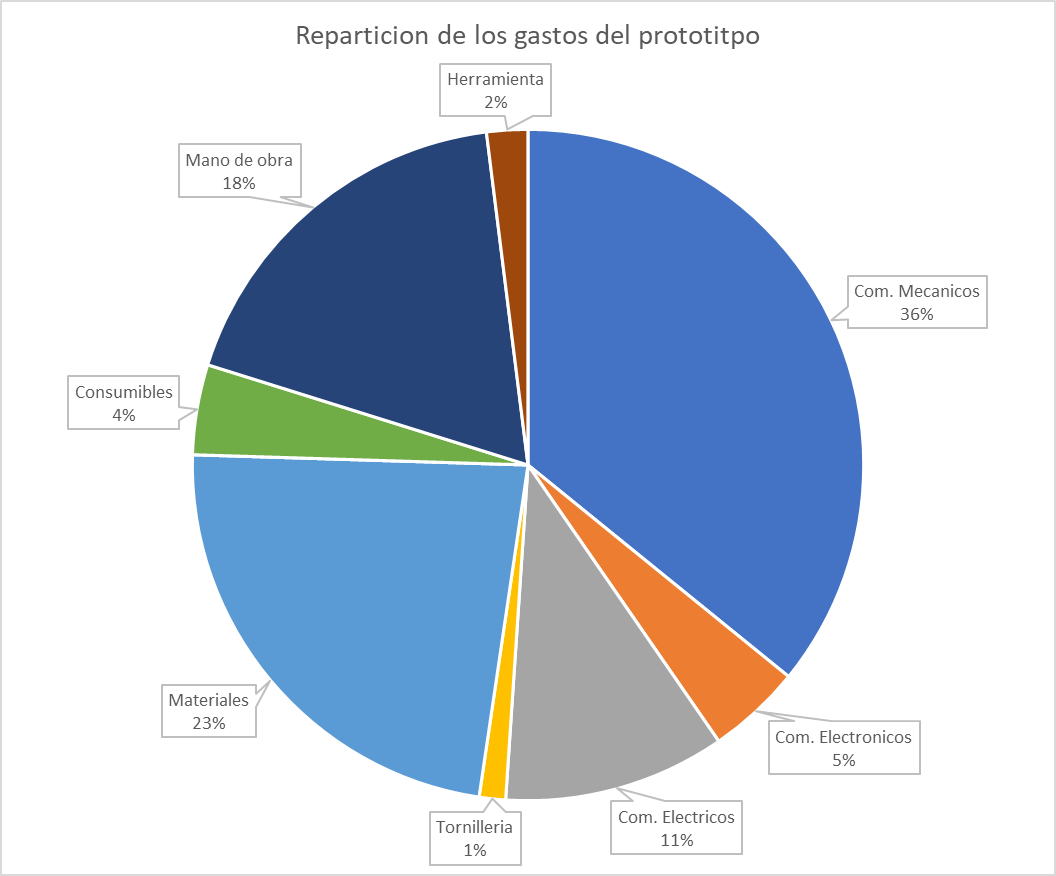
\includegraphics[scale=0.4]{images/Anexo/Reparticion_gastos.png}
        \caption{Repartición de los gastos}
    \label{fg:rep_gastos}
\end{figure}

\clearpage

\subsection{Valor de nuestro trabajo}

%\textbf{NOTA}: Aquí se mencionan los aportes que puede hacer nuestro trabajo y cual es su valor científico, social y cultural.

Este trabajo busca plantar un antecedente sobre los proyectos que se han realizado alrededor del aprovechamiento de los desechos orgánicos, integrando y enriqueciendo diversas ideas que se han realizado por separado, como se vieron en la tabla de antecedentes (Tabla \ref{tab:Tab_Antecedentes}).

De esta manera, se obtiene un sistema mas robusto, especializado para el tratamiento de los residuos vegetales y frutales, cuidando las condiciones del ambiente donde se realiza la maduración de los residuos, obteniendo resultados en 72 horas, que en otros tipos de procesos de compostaje, se obtienen en 2 meses.

Las dimensiones de este prototipo se pueden escalar, para aumentar su capacidad y poder beneficiar a diversas poblaciones, como lo pueden zonas habitacionales, edificios de departamentos, escuelas e incluso mercados. 

Aprovechando este tipo de recursos, se beneficia al ambiente, evitando la contaminación producida por el transporte y la descomposición de los desechos en  sanitarios. De igual forma, se busca cerrar el ciclo natural, devolviendo los nutrientes generados por las plantas y arboles, al suelo, para seguir produciendo vida.


%%%modificar archivo capitulos/discusion.tex
%%%%%%%%%%%%%%%%%%%%%%%%%%%%%%%%%%%%%%%%%%%%%%%%%%%%%%%%%%%%%%%%%%%
%%%Ajusta el contador de secciones y subsecciones para ete capítulo
\setcounter{secnumdepth}{-1}
%%%%%%%%%%%%%%%%%%%%%%%%%%%%%%%%%%%%%%%%%%%%%%%%%%%%%%%%%%%%%%%%%%%
% 2.4 Análisis de resultados
\chapter{Análisis de resultados}


\section{Propios del desarrollo tecnológico o investigación}

En este reporte de Trabajo Terminal I se tiene como objetivo principal realizar el diseño del sistema de compostaje, materializando una propuesta de diseño conceptual, construyendo y validando cada uno de los módulos que lo componen.

Para lograr este punto en general, se han realizado análisis  e investigaciones documentales previas que han ayudado a delimitar las opciones de soluciones tecnológicas a cada uno de los requerimientos y necesidades.

Una vez seleccionada cada una de las soluciones propuestas se ha realizado un análisis sobre las cuestiones que rodean a la solución, remarcando las ventajas y contrastándolas con las desventajas para sustentar la selección, también, de ser posible, se realizó una simulación para reforzar los argumentos de selección.

Las simulaciones se realizaron por medio de herramientas computacionales, utilizando el software de Matlab, Simulink, MD Solid y SolidWorks.

En este trabajo se han tomado en cuenta los conocimientos y las experiencias que se han obtenido a lo largo de la carrera, por lo cual, muchas de las soluciones y argumentos mostrados, cuentan con una visión de la ingeniería que se ha desarrollado a lo largo de la carrera.

Es por lo que, los diseños electrónicos son muy parecidos a diversos ejercicios y practicas que se han realizado durante algunas unidades de aprendizaje, por que ya se conoce su funcionamiento y en el proyecto se toman como una aplicación directa.

Estos sistemas electrónicos son los de monitoreo de la temperatura y de la humedad, también los circuito de activación de cada uno de los motores y la bomba de agua. Lo mismo pasa con la interfaz Humano - máquina y el uso de la tarjeta ESP32 para diversos proyectos de electrónica y control.

De esta manera se puede confiar en el funcionamiento de los circuitos propuestos, solo cuidando detalles en la manufactura de los PCB para evitar errores en las pistas y verificando que la impresión se haga de forma correcta para que cada componente electrónico esté instalado en el lugar donde le corresponde.

En caso de las leyes de control, en este caso se han utilizado simulaciones computacionales. En caso de los controles ON/OFF, la simulación no se realizo con mucho rigor debido a que es un control  sencillo que únicamente refleja un cambio de estado para activar o desactivar algún actuador del sistema.

Para la temperatura dento del contenedor, se realizó una simulación de un contenedor cerrado, siendo este sometido a diferentes estímulos térmicos, con los datos obtenidos en dicho experimento, se observa que la aplicación de un controlador PID es una buena opción para realizar el control de temperatura del compostador, además de tener en cuenta otras consideraciones para los fenómenos de las pérdidas de calor.

Estas consideraciones sobre las pérdidas de calor fueron una de las bases por las cuales se considero un rediseño del contenedor donde se llevará a cabo el proceso de compostaje, ya que este al estar expuesto al intemperie, especialmente a cambios de temperatura que afectan directamente al ambiente interno y por lo tanto, alterar el funcionamiento del monitoreo y de la activación de los actuadores.

Es por lo que se trabajó en la búsqueda de un material que aislara el contenedor del ambiente y conserve la temperatura a interior, para la cual se han realizado simulaciones de transferencia de calor con diversos materiales para conseguir el recubrimiento que más convenga de acuerdo a las necesidades del proyecto y se adapte a las condiciones ambientales de la Ciudad de México. Es importante mencionar que las pruebas realizadas con la fibra de vidrio, presentaron una reducción de la pérdida de calor de cinco veces con respecto al contenedor sin material aislante y permite mantener la temperatura de la cara externa un par de grados por encima de la temperatura ambiental. 

Por estas razones se cree que es viable realizar la construcción del contenedor, aún así, es necesario poder tener el contenedor construido y medianamente funcionando para poder realizar la correcta sintonización del controlador.

Por otro lado en cuanto a la ventilación de la cámara de compostaje, se realizaron algunas simulaciones proponiendo distintas distribuciones para los ventiladores en las que se observó cuál de ellas presentaba una distribución y recorrido uniforme del aire al interior del contenedor. 

Para el caso del eje del sistema de aireación se tomaron en cuenta diversas ideas para su elaboración. los principales detalles en el, fue la implementación de las palas con el mismo eje y que sea capaz de mover toda la carga propuesta. 

De esta manera, se decantó por un eje cilíndrico que atravesara de forma horizontal el contenedor, el cual estará perforado con unas roscas donde se van a colocar las palas planas. De esta forma se han realizado los estudios necesarios, donde el eje se somete a los diferentes momentos y cargas generadas durante su implementación.

De la simulación realizada, se destaca que el eje puede soportar esfuerzos de 33.5 Mpa y utilizando un acero ANSI 1045 con un limite elástico de 530 MPa, valida el diseño de eje propuesto y por lo que se puede pasar a su proceso de fabricación.

%no se que mas quieras poner en lo de trituración marco, esta bien man, si no ahorita a ver que mas le pongo, falta lo del puto impacto ambiental
%Tienes el documento de octavio donde habla de que es el impacto ambiental?, o esta en el teams? ya te lo mande por whats
Para el sistema de trituración se tomo en cuenta que sera una persona la encargada de imprimir el momento de torsión necesario para la trituración de la materia orgánica, por lo que fue necesario conocer la fuerza promedio que puede aplicar una persona, teniendo esos datos y una propuesta de utilizar un sistema de tornillo helicoidal y un rallador, se propuso seleccionar un dispositivo comercial que realizará una acción similar, por lo que se termino seleccionando un molino manual de carne, el cual mediante un tornillo helicoidal de paso variable y una cuchilla trituran la carne hasta dimensiones que se adaptan a nuestros requerimientos.

Con esta selección, se busco la manera de disminuir los procesos de fabricación requeridos durante la elaboración del proyecto, así como aprovechar mejor los tiempos que se disponen para la integración del sistema y sus pruebas.

En cuanto a la parte de la estructura, se realizaron simulaciones sobre un modelo de estructura convencional la cual estará encargada de soportar el peso de todos los componentes y la materia orgánica al interior del contenedor. 

Las validaciones numéricas se centraron en estudios estáticos, donde se busco observar como es que se reparte la carga de los componentes en toda la estructura y ver qué puntos son susceptibles a un fallo. 

Para validar los puntos críticos fue necesario calcular el esfuerzo máximo en esos puntos de apoyo y calcular el factor de seguridad de la estructura, en este caso el factor de seguridad ha sido de 31, el cual se ha considerado más que suficiente para el evitar problemas en la estructura.

También se observo que la deformación máxima en algunas vigas de la estructura, de tal forma que se puedan evitar deformaciones a largo plazo que puedan afectar el funcionamiento de todo el sistema o que provoque algún desperfecto en algún elemento mecánico.

Con los valores obtenidos, se observó que la estructura propuesta es una buena opción para llevar a cabo el proceso de compostaje, por lo tanto, este diseño se puede fabricar.
\section{Análisis de Costos}

En esta parte se realiza el desglose de los costos del proyecto, el cual está dividido en 3 partes, los materiales y componentes (Tabla \ref{tab:cost_mat}), las herramientas y equipo (Tabla \ref{tab:cost_herramientas}), y por último, la manufactura externa que será requerida (Tabla \ref{tab:cost_manodeobra}).

    \begin{table}[h!]
        \begin{center}
            \caption{Costos de materiales y componentes}
            \begin{tabular}{ | c | c | c | c | c |}
               \multicolumn{5}{c}{Material electrónico}\\ \hline
                Recurso & Unidad & Precio unitario & Total & Se cuenta con el  \\ \hline
                ESP32 & 1 & \$ 138.00 & \$ 138.00 & Si \\ \hline
                DHT11 & 1 & \$ 40.00 & \$ 40.00 & Si \\ \hline
                DS18B20  & 1 & \$ 45.00 & \$ 45.00 & Si  \\ \hline
                LCD 20X4 con I2C  & 1 & \$ 149.00 & \$ 149.00 & No  \\ \hline
                Push Button Grande  & 3 & \$ 4.00 & \$ 12.00 & No  \\ \hline
                Resistencias 1k  & 5 & \$ 1.00 & \$ 5.00 & Si  \\ \hline
                Header hembra 20 pines  & 2 & \$ 5.00 & \$ 10.00 & No  \\ \hline
                Headers macho 40 pines  & 1 & \$ 7.00 & \$ 7.00 & No  \\ \hline
                Bornera 2 terminales  & 2 & \$ 3.00 & \$ 6.00 & No  \\ \hline
                Bomba de agua  & 1 & \$ 32.00 & \$ 32.00 & No  \\ \hline
                Transistor TIP41  & 1 & \$ 17.00  & \$ 17.00 & Si  \\ \hline
                Ventilador PC a 12 V  & 2 & \$ 75.00 & \$ 150.00 & No  \\ \hline
                Relevadores 5V  & 4 & \$ 15.00 & \$ 60.00 & No  \\ \hline
                \multicolumn{5}{c}{Material eléctrico}\\ \hline
                Eliminador 5v  & 1 & \$ 80.00 & \$ 80.00 & Si  \\ \hline
                Eliminador 12v  & 1 & \$ 80.00 & \$ 80.00 & No  \\ \hline
                Fuente Conmutada 24 V a 10 A  & 1 & \$ 275.00 & \$ 275.00 & No  \\ \hline
                Resistencia calentador  & 10 & \$ 15.00 & \$ 150.00 & No  \\ \hline
                Multicontacto MUL-612X  & 1 & \$ 285.00 & \$ 285.00 & SI  \\ \hline
                \multicolumn{5}{c}{Metales}\\ \hline
                Perfil PTR 2X2 in calibre 14  & 4 & \$ 920.00 & \$ 3680.00 & No  \\ \hline
                Contenedor de acero laminado & 1 & \$ 3000.00 & \$ 3000.00  & No  \\ \hline
                Ángulo $\frac{1}{8}$ x 1 in  & 1 & \$ 358.00 & \$ 358.00 & No  \\ \hline
                \multicolumn{5}{c}{Materiales térmicos}\\ \hline
                Arcilla  & 2Kg & \$ 176.00 & \$ 352.00 & No  \\ \hline
                Fibra de vidrio  & 3Kg & \$ 452.00 & \$ 452.00 & No  \\ \hline
                \multicolumn{5}{c}{Componentes mecánicos}\\ \hline
                Triturador de carne  & 1 & \$ 1800.00 & \$ 1800.00 & No  \\ \hline
                Motorreductor NMRV040 & 1 & \$ 1600.00 A & \$ 1600.00 & No  \\ \hline
                Polea 11.35 in  & 1 & \$ 160.00 & \$ 160.00 & No  \\ \hline
                Polea 3.78 in  & 1 & \$ 80.00 & \$ 80.00 & No  \\ \hline
                Banda 3V 60 in  & 1 & \$ 250.00 & \$ 250.00 & No  \\ \hline
                Cuña $\frac{3}{8}$ x 2.5 in & 3 &  \$ 60.00& \$ 180.00 & No  \\ \hline
            \end{tabular}
            \label{tab:cost_mat}
        \end{center}
    \end{table}

    \begin{table}[h]
        \begin{center}
            \caption{Herramienta y equipo}
            \begin{tabular}{ | c | c | c | c | c |}
               \multicolumn{5}{c}{Equipo}\\ \hline
                Recurso & Unidad & \multicolumn{3}{|c|}{Se tiene acceso en:}  \\ \hline
                Cautin & 1 & \multicolumn{3}{|c|}{Casa} \\ \hline
                Planta soldadora & 1 & \multicolumn{3}{|c|}{Laboratorio de la UPIITA} \\ \hline
                Cortadora vertical & 1 & \multicolumn{3}{|c|}{En casa} \\ \hline
                \multicolumn{5}{c}{Herramienta}\\ \hline
                Recurso & Unidad & Precio unitario & Total & Se cuenta con el  \\ \hline
                Disco para cortar PTR & 2 & \$ 60.00 & \$ 120.00 & Si \\ \hline
                Soldadura de estaño & 2  & \$ 44.00 & \$ 88.00 & Si \\ \hline
                Electrodos para soldar Infra 2210 & 1kg & \$ 110.00 & \$ 110.00 & No \\ \hline                
            \end{tabular}
            \label{tab:cost_herramientas}
        \end{center}
    \end{table}

    \begin{table}[h]
        \begin{center}
            \caption{Manufactura externa}
            \begin{tabular}{ | c | c | c | c | c |}
               \multicolumn{4}{c}{Sistema de aeración}\\ \hline
                Recurso & Unidad & Precio unitario & Total & Tiempo de espera  \\ \hline
                Eje de aeración & 1 & \$ 2000.00 & \$ 2000.00 & 1 mes y 15 días \\ \hline
                Palas de aeración & 3 & \$ 600.00 & \$ 1800.00 & 1 mes\\ \hline
                \multicolumn{4}{c}{Sistemas electrónicos}\\ \hline
                Principal 10x10 cm  & 1 & \$ 435.00 & \$ 435.00 & 20 días  \\ \hline
                Botones 5x5 cm  & 1 & \$ 377.00 & \$ 377.00 & 20 días  \\ \hline
                Bomba de agua 5x5 cm  & 1 & \$ 377.00 & \$ 377.00 & 20 días  \\ \hline
                Control de ventiladores 5x5 cm  & 1 & \$ 377.00 & \$ 377.00  & 20 días \\ \hline
            \end{tabular}
            \label{tab:cost_manodeobra}
        \end{center}
    \end{table}

Ahora se realiza la suma total de los valores descritos en las tablas, por lo que se obtiene un costo tal que se muestra en la Tabla \ref{tab:gastototal}

\begin{table}[h]
        \begin{center}
            \caption{Gasto total}
            \begin{tabular}{ | c | c |}
               \hline
                Total & \$ 19137.00 \\ \hline
                \multicolumn{2}{|c|}{Diecinueve mil ciento treinta y siete pesos MXN}\\ \hline
            \end{tabular}
            \label{tab:gastototal}
        \end{center}
    \end{table}
  
%\subsection{}
\begin{comment}
    % Table generated by Excel2LaTeX from sheet 'Costos'
\begin{table}[h!]
  \centering
  \caption{Tabla de costos}
  \resizebox{18cm}{!}{
    \begin{tabular}{ccccccclc}
          &       &       &       &       &       &       &       &  \\
\cmidrule{2-8}    \multicolumn{1}{c|}{} & \multicolumn{1}{p{12.9em}|}{\cellcolor[rgb]{ .357,  .608,  .835}\textcolor[rgb]{ 1,  1,  1}{\textbf{Modulo}}} & \multicolumn{1}{p{12.9em}}{\cellcolor[rgb]{ .357,  .608,  .835}\textcolor[rgb]{ 1,  1,  1}{\textbf{Recurso }}} & \multicolumn{1}{p{4.3em}}{\cellcolor[rgb]{ .357,  .608,  .835}\textcolor[rgb]{ 1,  1,  1}{\textbf{Unidad}}} & \multicolumn{1}{p{5em}}{\cellcolor[rgb]{ .357,  .608,  .835}\textcolor[rgb]{ 1,  1,  1}{\textbf{Cantidad}}} & \multicolumn{1}{p{7.3em}}{\cellcolor[rgb]{ .357,  .608,  .835}\textcolor[rgb]{ 1,  1,  1}{\textbf{Precio unitario}}} & \multicolumn{1}{p{5.5em}}{\cellcolor[rgb]{ .357,  .608,  .835}\textcolor[rgb]{ 1,  1,  1}{\textbf{Total}}} & \multicolumn{1}{p{30.65em}|}{\cellcolor[rgb]{ .357,  .608,  .835}\textcolor[rgb]{ 1,  1,  1}{\textbf{Enlace}}} &  \\
\cmidrule{2-8}    \multicolumn{1}{c|}{} & \multicolumn{1}{p{12.9em}|}{\cellcolor[rgb]{ .867,  .922,  .969}\textbf{Sistema de Agitación}} & \multicolumn{1}{p{12.9em}}{\cellcolor[rgb]{ .867,  .922,  .969}\textbf{Chumaceras}} & \multicolumn{1}{p{4.3em}}{\cellcolor[rgb]{ .867,  .922,  .969}Pieza} & \cellcolor[rgb]{ .867,  .922,  .969}2 & \cellcolor[rgb]{ .867,  .922,  .969}\$105.00 & \cellcolor[rgb]{ .867,  .922,  .969}\$210.00 & \multicolumn{1}{p{30.65em}|}{\cellcolor[rgb]{ .867,  .922,  .969}\textcolor[rgb]{ .02,  .388,  .757}{https://articulo.mercadolibre.com.mx/MLM-724670234-chumacera-de-piso-34-pulgada-ucp204-12-\_JM\#position=1\&search\_layout=grid\&type=item\&tracking\_id=2b43f82e-2fe7-4ef9-ba2d-fbf004f4d955}} &  \\
\cmidrule{3-8}    \multicolumn{1}{c|}{} & \multicolumn{1}{r|}{\cellcolor[rgb]{ .867,  .922,  .969}} & \multicolumn{1}{p{12.9em}}{\textbf{Cold rolled 3/4" x 1 m}} & \multicolumn{1}{p{4.3em}}{Pieza} & 1     & \$550.00 & \$550.00 & \multicolumn{1}{p{30.65em}|}{\textcolor[rgb]{ .02,  .388,  .757}{https://articulo.mercadolibre.com.mx/MLM-948303783-barra-redonda-acero-cold-rolled-1045-34-100cm-\_JM\#position=1\&search\_layout=stack\&type=item\&tracking\_id=d256e578-507b-4987-8afd-6e45742d6da6}} &  \\
\cmidrule{3-8}    \multicolumn{1}{c|}{} & \multicolumn{1}{r|}{\cellcolor[rgb]{ .867,  .922,  .969}} & \multicolumn{1}{p{12.9em}}{\cellcolor[rgb]{ .867,  .922,  .969}\textbf{Motoreductor}} & \multicolumn{1}{p{4.3em}}{\cellcolor[rgb]{ .867,  .922,  .969}Pieza} & \cellcolor[rgb]{ .867,  .922,  .969}1 & \cellcolor[rgb]{ .867,  .922,  .969}\$6,120.00 & \cellcolor[rgb]{ .867,  .922,  .969}\$6,120.00 & \multicolumn{1}{p{30.65em}|}{\cellcolor[rgb]{ .867,  .922,  .969}\textcolor[rgb]{ .02,  .388,  .757}{https://articulo.mercadolibre.com.mx/MLM-626833172-reductor-de-velocidad-para-motor-nmrv063-\_JM}} &  \\
\cmidrule{3-8}    \multicolumn{1}{c|}{} & \multicolumn{1}{r|}{\cellcolor[rgb]{ .867,  .922,  .969}} & \multicolumn{1}{p{12.9em}}{\textbf{Motor }} & \multicolumn{1}{p{4.3em}}{Pieza} & 1     & \$2,199.00 & \$2,199.00 & \multicolumn{1}{p{30.65em}|}{\textcolor[rgb]{ .02,  .388,  .757}{https://articulo.mercadolibre.com.mx/MLM-589353082-motor-monofasico-de-12-hp-baja-siemens-uso-general-\_JM\#position=3\&search\_layout=grid\&type=item\&tracking\_id=b149ef04-f061-4058-a158-317d50b0a93b}} &  \\
\cmidrule{3-8}    \multicolumn{1}{c|}{} & \multicolumn{1}{r|}{\cellcolor[rgb]{ .867,  .922,  .969}} & \multicolumn{1}{p{12.9em}}{\cellcolor[rgb]{ .867,  .922,  .969}\textbf{Aspas}} & \multicolumn{1}{p{4.3em}}{\cellcolor[rgb]{ .867,  .922,  .969}Pieza} & \cellcolor[rgb]{ .867,  .922,  .969}3 & \cellcolor[rgb]{ .867,  .922,  .969}\$288.00 & \cellcolor[rgb]{ .867,  .922,  .969}\$864.00 & \multicolumn{1}{p{30.65em}|}{\cellcolor[rgb]{ .867,  .922,  .969}\textcolor[rgb]{ .02,  .388,  .757}{https://articulo.mercadolibre.com.mx/MLM-1434856531-varilla-lisa-redondo-acero-inoxidable-de-12-x-1-metro-\_JM\#position=2\&search\_layout=grid\&type=item\&tracking\_id=e4d9d31a-028d-430e-a703-e49f5a64c7d1}} &  \\
\cmidrule{2-8}    \multicolumn{1}{c|}{} & \multicolumn{1}{p{12.9em}|}{\textbf{Sistema de trituración}} & \multicolumn{1}{p{12.9em}}{\textbf{chuchillas de molienda}} & \multicolumn{1}{p{4.3em}}{Pieza} & 2     & \$240.00 & \$480.00 & \multicolumn{1}{p{30.65em}|}{\textcolor[rgb]{ .02,  .388,  .757}{https://articulo.mercadolibre.com.mx/MLM-1419905171-cuchillas-de-molienda-de-gusano-de-molienda-de-1-pieza-\_JM?matt\_tool=47634512\&matt\_word=\&matt\_source=google\&matt\_campaign\_id=15700894058\&matt\_ad\_group\_id=145960969852\&matt\_match\_type=\&matt\_network=g\&matt\_device=c\&matt\_creative=619538684828\&matt\_keyword=\&matt\_ad\_position=\&matt\_ad\_type=pla\&matt\_merchant\_id=284348069\&matt\_product\_id=MLM1419905171\&matt\_product\_partition\_id=1730485668402\&matt\_target\_id=pla-1730485668402\&gclid=CjwKCAiAkfucBhBBEiwAFjbkr-l0mCLqOiHfTLakDVXRgD1j9WVU7dQ4nfBrp1QICZG7meqf7wPuKBoCzroQAvD\_BwE}} &  \\
\cmidrule{2-8}    \multicolumn{1}{c|}{} & \multicolumn{1}{p{12.9em}|}{\cellcolor[rgb]{ .867,  .922,  .969}\textbf{Estructura}} & \multicolumn{1}{p{12.9em}}{\cellcolor[rgb]{ .867,  .922,  .969}\textbf{Contenedor Metálico de 114 litros}} & \cellcolor[rgb]{ .867,  .922,  .969}Pieza & \cellcolor[rgb]{ .867,  .922,  .969}1 & \cellcolor[rgb]{ .867,  .922,  .969}\$3,036.00  & \cellcolor[rgb]{ .867,  .922,  .969}\$3,036.00  & \multicolumn{1}{p{30.65em}|}{\cellcolor[rgb]{ .867,  .922,  .969}\textcolor[rgb]{ .02,  .388,  .757}{https://es.uline.mx/Product/Detail/S-14365/Drums/Steel-Drum-30-Gallon-Closed-Top-Unlined}} &  \\
\cmidrule{3-8}    \multicolumn{1}{c|}{} & \multicolumn{1}{r|}{\cellcolor[rgb]{ .867,  .922,  .969}} & \multicolumn{1}{p{12.9em}}{\textbf{PTR 2x2 c-18 (6 metros)}} & \multicolumn{1}{p{4.3em}}{Pieza} & 2     & \$650.00 & \$1,300.00 & \multicolumn{1}{p{30.65em}|}{\textcolor[rgb]{ .02,  .388,  .757}{https://www.construrama.com/materialesverduzco/catalogo/aceros/acero-estructural/perfiles/perfil-tubular-cuadrado-2-x-2-c18-6-m-pieza/p/0205010310}} &  \\
\cmidrule{3-8}    \multicolumn{1}{c|}{} & \multicolumn{1}{r|}{\cellcolor[rgb]{ .867,  .922,  .969}} & \multicolumn{1}{p{12.9em}}{\cellcolor[rgb]{ .867,  .922,  .969}\textbf{Regatón cuadrado 2x2}} & \multicolumn{1}{p{4.3em}}{\cellcolor[rgb]{ .867,  .922,  .969}Paquete} & \cellcolor[rgb]{ .867,  .922,  .969}1 & \cellcolor[rgb]{ .867,  .922,  .969}\$489.00 & \cellcolor[rgb]{ .867,  .922,  .969}\$489.00 & \multicolumn{1}{p{30.65em}|}{\cellcolor[rgb]{ .867,  .922,  .969}\textcolor[rgb]{ .02,  .388,  .757}{https://www.amazon.com.mx/dp/B07XLBSC96/ref=sspa\_dk\_detail\_0?pd\_rd\_i=B07XRQ9VQG\&pd\_rd\_w=t4TPG\&content-id=amzn1.sym.f9db214f-45b5-4f3b-8f3e-c2b60dfd9e46\&pf\_rd\_p=f9db214f-45b5-4f3b-8f3e-c2b60dfd9e46\&pf\_rd\_r=MTT70BHX6Y21FH8G0C0Z\&pd\_rd\_wg=NcF87\&pd\_rd\_r=76e6c457-d7c8-44dc-9f38-6048a742bc67\&s=tools\&sp\_csd=d2lkZ2V0TmFtZT1zcF9kZXRhaWw\&th=1}} &  \\
\cmidrule{3-8}    \multicolumn{1}{c|}{} & \multicolumn{1}{r|}{\cellcolor[rgb]{ .867,  .922,  .969}} & \multicolumn{1}{p{12.9em}}{\textbf{Electrodos de soldadura}} & \multicolumn{1}{p{4.3em}}{Paquete} & 1     & \$103.00 & \$103.00 & \multicolumn{1}{p{30.65em}|}{\textcolor[rgb]{ .02,  .388,  .757}{https://www.amazon.com.mx/Truper-E7018-4-Electrodo-7018-bolsa/dp/B013R1140I/ref=asc\_df\_B013R1140I/?tag=gledskshopmx-20\&linkCode=df0\&hvadid=547188937369\&hvpos=\&hvnetw=g\&hvrand=16262410558310842416\&hvpone=\&hvptwo=\&hvqmt=\&hvdev=c\&hvdvcmdl=\&hvlocint=\&hvlocphy=1010095\&hvtargid=pla-1595748632762\&th=1}} &  \\
\cmidrule{3-8}    \multicolumn{1}{c|}{} & \multicolumn{1}{r|}{\cellcolor[rgb]{ .867,  .922,  .969}} & \multicolumn{1}{p{12.9em}}{\cellcolor[rgb]{ .867,  .922,  .969}\textbf{Bisagras}} & \multicolumn{1}{p{4.3em}}{\cellcolor[rgb]{ .867,  .922,  .969}Paquete} & \cellcolor[rgb]{ .867,  .922,  .969}1 & \cellcolor[rgb]{ .867,  .922,  .969}\$360.00 & \cellcolor[rgb]{ .867,  .922,  .969}\$360.00 & \multicolumn{1}{p{30.65em}|}{\cellcolor[rgb]{ .867,  .922,  .969}\textcolor[rgb]{ .02,  .388,  .757}{https://www.amazon.com.mx/bnafes-Bisagra-armario-plástico-unidades/dp/B09LD5X185/ref=asc\_df\_B09LD5X185/?tag=gledskshopmx-20\&linkCode=df0\&hvadid=547107025881\&hvpos=\&hvnetw=g\&hvrand=17007795311563221941\&hvpone=\&hvptwo=\&hvqmt=\&hvdev=c\&hvdvcmdl=\&hvlocint=\&hvlocphy=1010095\&hvtargid=pla-1598654234520\&psc=1}} &  \\
\cmidrule{3-8}    \multicolumn{1}{c|}{} & \multicolumn{1}{r|}{\cellcolor[rgb]{ .867,  .922,  .969}} & \multicolumn{1}{p{12.9em}}{\textbf{Tornillos}} & \multicolumn{1}{p{4.3em}}{Paquete} & 1     & \$78.00 & \$78.00 & \multicolumn{1}{p{30.65em}|}{\textcolor[rgb]{ .02,  .388,  .757}{https://www.amazon.com.mx/FIERO-PIJ-825-Fiero-Pija-25/dp/B013SF1BYW/ref=asc\_df\_B013SF1BYW/?tag=gledskshopmx-20\&linkCode=df0\&hvadid=360862795141\&hvpos=\&hvnetw=g\&hvrand=2754026132586988086\&hvpone=\&hvptwo=\&hvqmt=\&hvdev=c\&hvdvcmdl=\&hvlocint=\&hvlocphy=1010095\&hvtargid=pla-383309711753\&psc=1}} &  \\
\cmidrule{3-8}    \multicolumn{1}{c|}{} & \multicolumn{1}{r|}{\cellcolor[rgb]{ .867,  .922,  .969}} & \multicolumn{1}{p{12.9em}}{\cellcolor[rgb]{ .867,  .922,  .969}\textbf{Pernos}} & \multicolumn{1}{p{4.3em}}{\cellcolor[rgb]{ .867,  .922,  .969}Paquete} & \cellcolor[rgb]{ .867,  .922,  .969}1 & \cellcolor[rgb]{ .867,  .922,  .969}\$314.00 & \cellcolor[rgb]{ .867,  .922,  .969}\$314.00 & \multicolumn{1}{p{30.65em}|}{\cellcolor[rgb]{ .867,  .922,  .969}\textcolor[rgb]{ .02,  .388,  .757}{https://www.elektra.mx/tor5-1-2-x2-1-2-tornillo-grado-5-1-2-x-2-1-2-1500511729/p?gclid=Cj0KCQjw3a2iBhCFARIsAD4jQB1UZAStPDonbn5w0qta2jq5ReaxiBoDz0PL\_J343zC853sG-mOHfkcaAtb2EALw\_wcB}} &  \\
\cmidrule{3-8}    \multicolumn{1}{c|}{} & \multicolumn{1}{r|}{\cellcolor[rgb]{ .867,  .922,  .969}} & \multicolumn{1}{p{12.9em}}{\textbf{Rondanas}} & \multicolumn{1}{p{4.3em}}{Paquete} & 1     & \$79.00 & \$79.00 & \multicolumn{1}{p{30.65em}|}{\textcolor[rgb]{ .02,  .388,  .757}{https://www.homedepot.com.mx/ferreteria/ferreteria-general/tornillos-tuercas-y-arandelas/arandela-plana-no-8-10p-815995?gclid=Cj0KCQiAyMKbBhD1ARIsANs7rEHx6ZBeVGsazztxgeSo0tDVIVQS\_phWmyHFI8Lo0AOuG8JSn1ZeP54aAokREALw\_wcB\&gclsrc=aw.ds}} &  \\
\cmidrule{3-8}    \multicolumn{1}{c|}{} & \multicolumn{1}{r|}{\cellcolor[rgb]{ .867,  .922,  .969}} & \multicolumn{1}{p{12.9em}}{\cellcolor[rgb]{ .867,  .922,  .969}\textbf{Tuercas}} & \multicolumn{1}{p{4.3em}}{\cellcolor[rgb]{ .867,  .922,  .969}Paquete} & \cellcolor[rgb]{ .867,  .922,  .969}2 & \cellcolor[rgb]{ .867,  .922,  .969}\$139.00 & \cellcolor[rgb]{ .867,  .922,  .969}\$278.00 & \multicolumn{1}{p{30.65em}|}{\cellcolor[rgb]{ .867,  .922,  .969}\textcolor[rgb]{ .02,  .388,  .757}{https://www.homedepot.com.mx/tornillos-tuercas-y-arandelas/tuerca-hexagonal-acero-inoxidable-1-2-13-816365}} &  \\
\cmidrule{2-8}    \multicolumn{1}{c|}{} & \multicolumn{1}{p{12.9em}|}{\textbf{Alimentación y protección electrica}} & \multicolumn{1}{p{12.9em}}{\textbf{Fusibles}} & \multicolumn{1}{p{4.3em}}{Paquete} & 1     & \$39.00 & \$39.00 & \multicolumn{1}{p{30.65em}|}{\textcolor[rgb]{ .02,  .388,  .757}{https://www.homedepot.com.mx/electrico/centros-de-carga-e-interruptores/centros-de-carga-y-fusibles/fusible-americano-5pzas-vidrio-443570?gclid=Cj0KCQiAyMKbBhD1ARIsANs7rEF6x\_7KC0Dwrt6dySyAhwSVVjHm9Tg8ANkspryyY9FOKjNIl8XsYTUaAvA\_EALw\_wcB\&gclsrc=aw.ds}} &  \\
\cmidrule{3-8}    \multicolumn{1}{c|}{} & \multicolumn{1}{r|}{} & \multicolumn{1}{p{12.9em}}{\cellcolor[rgb]{ .867,  .922,  .969}\textbf{Pastilla}} & \multicolumn{1}{p{4.3em}}{\cellcolor[rgb]{ .867,  .922,  .969}pieza} & \cellcolor[rgb]{ .867,  .922,  .969}1 & \cellcolor[rgb]{ .867,  .922,  .969}\$193.00 & \cellcolor[rgb]{ .867,  .922,  .969}\$193.00 & \multicolumn{1}{p{30.65em}|}{\cellcolor[rgb]{ .867,  .922,  .969}\textcolor[rgb]{ .02,  .388,  .757}{https://www.amazon.com.mx/Schneider-Electric-QO130-Interruptor-Termomagnético/dp/B000CCSPRQ/ref=asc\_df\_B000CCSPRQ/?tag=gledskshopmx-20\&linkCode=df0\&hvadid=295433315443\&hvpos=\&hvnetw=g\&hvrand=10746481071746106372\&hvpone=\&hvptwo=\&hvqmt=\&hvdev=c\&hvdvcmdl=\&hvlocint=\&hvlocphy=1010095\&hvtargid=pla-451056876938\&psc=1}} &  \\
\cmidrule{3-8}    \multicolumn{1}{c|}{} & \multicolumn{1}{r|}{} & \multicolumn{1}{p{12.9em}}{\textbf{Clavija uso rudo}} & \multicolumn{1}{p{4.3em}}{Pieza} & 1     & \$263.00 & \$263.00 & \multicolumn{1}{p{30.65em}|}{\textcolor[rgb]{ .02,  .388,  .757}{https://www.amazon.com.mx/Leviton-2321-20-Amp-enchufe-Industrial-Black-White/dp/B000PDBLP0/ref=asc\_df\_B000PDBLP0/?tag=gledskshopmx-20\&linkCode=df0\&hvadid=450913306012\&hvpos=\&hvnetw=g\&hvrand=2461479506740344671\&hvpone=\&hvptwo=\&hvqmt=\&hvdev=c\&hvdvcmdl=\&hvlocint=\&hvlocphy=1010095\&hvtargid=pla-312341928661\&psc=1}} &  \\
\cmidrule{3-8}    \multicolumn{1}{c|}{} & \multicolumn{1}{r|}{} & \multicolumn{1}{p{12.9em}}{\cellcolor[rgb]{ .867,  .922,  .969}\textbf{Cable de alimentacion uso rudo}} & \multicolumn{1}{p{4.3em}}{\cellcolor[rgb]{ .867,  .922,  .969}Pieza} & \cellcolor[rgb]{ .867,  .922,  .969}1 & \cellcolor[rgb]{ .867,  .922,  .969}\$625.00 & \cellcolor[rgb]{ .867,  .922,  .969}\$625.00 & \multicolumn{1}{p{30.65em}|}{\cellcolor[rgb]{ .867,  .922,  .969}\textcolor[rgb]{ .02,  .388,  .757}{https://www.amazon.com.mx/Supplying-Demand-compatible-Whirlpool-Frigidaire/dp/B07S95JMZN/ref=asc\_df\_B07SB6SP65/?tag=gledskshopmx-20\&linkCode=df0\&hvadid=531699563514\&hvpos=\&hvnetw=g\&hvrand=14612895901489646193\&hvpone=\&hvptwo=\&hvqmt=\&hvdev=c\&hvdvcmdl=\&hvlocint=\&hvlocphy=1010095\&hvtargid=pla-781979566996\&th=1}} &  \\
\cmidrule{3-8}    \multicolumn{1}{c|}{} & \multicolumn{1}{r|}{} & \multicolumn{1}{p{12.9em}}{\textbf{Cable electrico 22AWG}} & \multicolumn{1}{p{4.3em}}{Pieza} & 1     & \$450.00 & \$450.00 & \multicolumn{1}{p{30.65em}|}{\textcolor[rgb]{ .02,  .388,  .757}{https://www.amazon.com.mx/eléctrico-conductores-extensión-revestimiento-iluminación/dp/B08QJ23K5V/ref=asc\_df\_B08QJ23K5V/?tag=gledskshopmx-20\&linkCode=df0\&hvadid=547456034291\&hvpos=\&hvnetw=g\&hvrand=5094219301240143337\&hvpone=\&hvptwo=\&hvqmt=\&hvdev=c\&hvdvcmdl=\&hvlocint=\&hvlocphy=1010095\&hvtargid=pla-1162146297344\&psc=1}} &  \\
\cmidrule{3-8}    \multicolumn{1}{c|}{} & \multicolumn{1}{r|}{} & \multicolumn{1}{p{12.9em}}{\cellcolor[rgb]{ .867,  .922,  .969}\textbf{Fuente conmutada}} & \multicolumn{1}{p{4.3em}}{\cellcolor[rgb]{ .867,  .922,  .969}Pieza} & \cellcolor[rgb]{ .867,  .922,  .969}1 & \cellcolor[rgb]{ .867,  .922,  .969}\$103.00 & \cellcolor[rgb]{ .867,  .922,  .969}\$103.00 & \multicolumn{1}{p{30.65em}|}{\cellcolor[rgb]{ .867,  .922,  .969}\textcolor[rgb]{ .02,  .388,  .757}{https://uelectronics.com/producto/fuente-conmutada-5v-3a/}} &  \\
\cmidrule{2-8}    \multicolumn{1}{c|}{} & \multicolumn{1}{p{12.9em}|}{\cellcolor[rgb]{ .867,  .922,  .969}\textbf{Sistema de Escape}} & \multicolumn{1}{p{12.9em}}{\textbf{Biofiltro}} & \multicolumn{1}{p{4.3em}}{Pieza} & 1     & \$1,035.00 & \$1,035.00 & \multicolumn{1}{p{30.65em}|}{\textcolor[rgb]{ .02,  .388,  .757}{https://www.amazon.com.mx/Filtro-carbono-pulgadas-para-filtración/dp/B07VKJG4DQ/ref=asc\_df\_B07VKJG4DQ/?tag=gledskshopmx-20\&linkCode=df0\&hvadid=431306202928\&hvpos=\&hvnetw=g\&hvrand=16078185325131603985\&hvpone=\&hvptwo=\&hvqmt=\&hvdev=c\&hvdvcmdl=\&hvlocint=\&hvlocphy=1010095\&hvtargid=pla-820573004140\&psc=1}} &  \\
\cmidrule{2-8}    \multicolumn{1}{c|}{} & \multicolumn{1}{p{12.9em}|}{\textbf{Sistema de control variables internas}} & \multicolumn{1}{p{12.9em}}{\cellcolor[rgb]{ .867,  .922,  .969}\textbf{Resistencias}} & \multicolumn{1}{p{4.3em}}{\cellcolor[rgb]{ .867,  .922,  .969}Pieza} & \cellcolor[rgb]{ .867,  .922,  .969}2 & \cellcolor[rgb]{ .867,  .922,  .969}\$298.00 & \cellcolor[rgb]{ .867,  .922,  .969}\$596.00 & \multicolumn{1}{p{30.65em}|}{\cellcolor[rgb]{ .867,  .922,  .969}\textcolor[rgb]{ .02,  .388,  .757}{https://articulo.mercadolibre.com.mx/MLM-805926887-resistencia-calentadora-para-incubadora-15-cm-\_JM?matt\_tool=28238160\&utm\_source=google\_shopping\&utm\_medium=organic}} &  \\
\cmidrule{3-8}    \multicolumn{1}{c|}{} & \multicolumn{1}{r|}{} & \multicolumn{1}{p{12.9em}}{\textbf{Ventilador }} & \multicolumn{1}{p{4.3em}}{Pieza} & 1     & \$350.00 & \$350.00 & \multicolumn{1}{p{30.65em}|}{\textcolor[rgb]{ .02,  .388,  .757}{https://www.amazon.com.mx/Noctua-NF-P12-PWM-Rendimiento-1700/dp/B07CG2PGY6/ref=asc\_df\_B07CG2PGY6/?tag=gledskshopmx-20\&linkCode=df0\&hvadid=360449982437\&hvpos=\&hvnetw=g\&hvrand=4181831070576725794\&hvpone=\&hvptwo=\&hvqmt=\&hvdev=c\&hvdvcmdl=\&hvlocint=\&hvlocphy=1010095\&hvtargid=pla-525425972873\&psc=1}} &  \\
\cmidrule{3-8}    \multicolumn{1}{c|}{} & \multicolumn{1}{r|}{} & \multicolumn{1}{p{12.9em}}{\cellcolor[rgb]{ .867,  .922,  .969}\textbf{Sensores de deteccion}} & \multicolumn{1}{p{4.3em}}{\cellcolor[rgb]{ .867,  .922,  .969}Pieza} & \cellcolor[rgb]{ .867,  .922,  .969}3 & \cellcolor[rgb]{ .867,  .922,  .969}\$51.00 & \cellcolor[rgb]{ .867,  .922,  .969}\$153.00 & \multicolumn{1}{p{30.65em}|}{\cellcolor[rgb]{ .867,  .922,  .969}\textcolor[rgb]{ .02,  .388,  .757}{https://uelectronics.com/categoria-producto/sensores/gas/}} &  \\
\cmidrule{2-8}    \multicolumn{1}{c|}{} & \multicolumn{1}{p{12.9em}|}{\cellcolor[rgb]{ .867,  .922,  .969}\textbf{Modulo Interfaz Humano-Maquina}} & \multicolumn{1}{p{12.9em}}{\textbf{Tarjeta de Desarrollo}} & \multicolumn{1}{p{4.3em}}{Pieza} & 1     & \$640.00 & \$640.00 & \multicolumn{1}{p{30.65em}|}{\textcolor[rgb]{ .02,  .388,  .757}{https://www.amazon.com.mx/Arduino-Org-A000066-R3-microcontrolador-a000066/dp/B008GRTSV6/ref=asc\_df\_B008GRTSV6/?tag=gledskshopmx-20\&linkCode=df0\&hvadid=339643974669\&hvpos=\&hvnetw=g\&hvrand=12094881554458557989\&hvpone=\&hvptwo=\&hvqmt=\&hvdev=c\&hvdvcmdl=\&hvlocint=\&hvlocphy=1010095\&hvtargid=pla-457497319401\&psc=1}} &  \\
\cmidrule{3-8}    \multicolumn{1}{c|}{} & \multicolumn{1}{r|}{\cellcolor[rgb]{ .867,  .922,  .969}} & \multicolumn{1}{p{12.9em}}{\cellcolor[rgb]{ .867,  .922,  .969}\textbf{Botones}} & \multicolumn{1}{p{4.3em}}{\cellcolor[rgb]{ .867,  .922,  .969}Pieza} & \cellcolor[rgb]{ .867,  .922,  .969}4 & \cellcolor[rgb]{ .867,  .922,  .969}\$60.00 & \cellcolor[rgb]{ .867,  .922,  .969}\$240.00 & \multicolumn{1}{p{30.65em}|}{\cellcolor[rgb]{ .867,  .922,  .969}\textcolor[rgb]{ .02,  .388,  .757}{https://articulo.mercadolibre.com.mx/MLM-551237268-boton-pulsador-verde-22mm-segetek-\_JM?matt\_tool=47634512\&matt\_word=\&matt\_source=google\&matt\_campaign\_id=15700894058\&matt\_ad\_group\_id=145960969852\&matt\_match\_type=\&matt\_network=g\&matt\_device=c\&matt\_creative=619538684828\&matt\_keyword=\&matt\_ad\_position=\&matt\_ad\_type=pla\&matt\_merchant\_id=465951677\&matt\_product\_id=MLM551237268\&matt\_product\_partition\_id=1731089326466\&matt\_target\_id=pla-1731089326466\&gclid=Cj0KCQiAyMKbBhD1ARIsANs7rEFKk6VvxTdclEHWzdAOEVepqUBw0XOZQiPuqjYP3xl7ZGW1etqOPpoaAoHcEALw\_wcB}} &  \\
\cmidrule{3-8}    \multicolumn{1}{c|}{} & \multicolumn{1}{r|}{\cellcolor[rgb]{ .867,  .922,  .969}} & \multicolumn{1}{p{12.9em}}{\textbf{Pantalla}} & \multicolumn{1}{p{4.3em}}{Pieza} & 1     & \$259.00 & \$259.00 & \multicolumn{1}{p{30.65em}|}{\textcolor[rgb]{ .02,  .388,  .757}{https://www.amazon.com.mx/Ymiko-pantalla-pulgadas-480x320-Arduino/dp/B08KDLJ9H7/ref=dp\_fod\_2?pd\_rd\_w=HmysX\&content-id=amzn1.sym.d503d5ce-f6c3-450d-8a24-dfaf868977bf\&pf\_rd\_p=d503d5ce-f6c3-450d-8a24-dfaf868977bf\&pf\_rd\_r=3WH861SYKAB2827WAERF\&pd\_rd\_wg=bdf7f\&pd\_rd\_r=ec63661f-1e08-402a-b1eb-fc4044280b4f\&pd\_rd\_i=B08KDLJ9H7\&th=1}} &  \\
\cmidrule{2-8}    \multicolumn{1}{c|}{} & \multicolumn{1}{p{12.9em}|}{\textbf{Programacion y diseño del sistema}} & \multicolumn{1}{p{12.9em}}{\cellcolor[rgb]{ .867,  .922,  .969}\textbf{Computadora}} & \multicolumn{1}{p{4.3em}}{\cellcolor[rgb]{ .867,  .922,  .969}Pieza} & \cellcolor[rgb]{ .867,  .922,  .969}1 & \multicolumn{1}{p{7.3em}}{\cellcolor[rgb]{ .867,  .922,  .969}Ya se tiene} & \cellcolor[rgb]{ .867,  .922,  .969} & \multicolumn{1}{l|}{\cellcolor[rgb]{ .867,  .922,  .969}} &  \\
\cmidrule{3-8}    \multicolumn{1}{c|}{} & \multicolumn{1}{r|}{} & \multicolumn{1}{p{12.9em}}{\textbf{Software CAD}} & \multicolumn{1}{p{4.3em}}{Pieza} & 1     & \multicolumn{1}{p{7.3em}}{Licencia Escolar} &       & \multicolumn{1}{l|}{} &  \\
\cmidrule{2-8}    \multicolumn{1}{c|}{} & \multicolumn{1}{c|}{} & \multicolumn{1}{p{12.9em}}{\cellcolor[rgb]{ .867,  .922,  .969}\textbf{Banco de herramientas}} & \multicolumn{1}{p{4.3em}}{\cellcolor[rgb]{ .867,  .922,  .969}Pieza} & \cellcolor[rgb]{ .867,  .922,  .969}1 & \multicolumn{1}{p{7.3em}}{\cellcolor[rgb]{ .867,  .922,  .969}Escuela} & \cellcolor[rgb]{ .867,  .922,  .969} & \multicolumn{1}{l|}{\cellcolor[rgb]{ .867,  .922,  .969}} &  \\
\cmidrule{2-8}    \multicolumn{1}{c|}{} & \multicolumn{1}{c|}{\cellcolor[rgb]{ .867,  .922,  .969}} &       &       &       & \textbf{Total:} & \textbf{\$21,406.00} & \multicolumn{1}{l|}{} &  \\
\cmidrule{2-8}          &       &       &       &       &       &       &       &  \\
    \end{tabular}%
    }
  \label{tab:costos}%
\end{table}%
\end{comment}


\newpage
\clearpage
\section{Impacto ambiental}

Al realizar el análisis del impacto ambiental, se considera que la fabricación del dispositivo tendrá un impacto reducido, debido a que se optó por adquirir y ensamblar productos y piezas que ya se encuentran disponibles en el mercado. De esta manera, se busca disminuir la cantidad de procesos de manufactura necesarios para su construcción.

Al mismo tiempo, se utilizan materiales y componentes que se puedan obtener en las cercanías del Valle de México, para evitar envíos largos y disminuir la huella de carbono que estos trayectos generarían en el ambiente.

Se prevé que el consumo de energía eléctrica que demande el dispositivo sea algo alto, debido a la potencia consumida por las resistencias del sistema de temperatura y por la potencia demandada por el motor del eje de aireación. A su vez, se busca disminuir el impacto en el consumo de energía, optimizando las condiciones ambientales del contenedor, siendo, de esta forma, un recubrimiento térmico aislante una opción amigable con el medio ambiente, ya que reduce en gran medida el consumo eléctrico utilizado para mantener una temperatura constante en el sistema.

De esta forma, se busca generar un ambiente constante dentro del contenedor para que el uso de los actuadores de temperatura y aireación se utilicen lo menos posible, reduciendo el impacto negativo del sistema.

Por otra parte, siendo este un sistema que busca reducir el impacto ambiental generado por las plantas de compostaje tradicionales, eliminando la necesidad de transportar los residuos a un lugar especializado para su procesamiento y mejorando el aprovechamiento del producto obtenido.

Esto, en conjunto, nos genera un impacto ambiental menor y ayuda a disminuir una problemática ambiental que nos afecta hoy en día: el transporte y mal aprovechamiento de los residuos orgánicos.

En un principio, este proyecto tenía como objetivo procesar los residuos orgánicos generados en la cafetería escolar. Sin embargo, la cantidad de residuos producidos requería un sistema de mayores dimensiones, lo que implicaba un costo que excedía el presupuesto disponible para el proyecto. A pesar de ello, si fuera posible desarrollar un sistema con la capacidad de procesar la totalidad de estos residuos y replicarlo en cada escuela del Instituto Politécnico Nacional, se podría generar un impacto positivo significativo en la reducción de la contaminación y en el aprovechamiento de los residuos orgánicos generados en la Ciudad de México.
\clearpage
\section{Sustentabilidad}

El proyecto tiene como objetivo procesar los desechos vegetales y frutales generados en una casa, por lo cual se aprovechan para crear abono casero para plantas o que puede ser aprovechado para áreas verdes públicas. Esto en miras de los objetivos ambientales que se tienen dentro de la Ciudad de México.

También se abre como una opción que busca estar al alcance de la gente para que se integre en las tareas de reutilización de recursos, generando un dispositivo que sea accesible y que se pueda adaptar en una casa común dentro del Valle de México.

El diseño del prototipo está previsto para ser manipulado por jóvenes y adultos, debido a que el sistema de trituración se encuentra expuesto y el sistema de regulación de temperatura puede representar un riesgo para los niños. Sin embargo, se contemplaron las condiciones necesarias para que una persona externa pueda operar el dispositivo de manera segura y, al mismo tiempo, participar en el proceso de compostaje.

Con su implementación, se busca tener un impacto ecológico positivo al realizar el procesamiento y aprovechamiento de residuos orgánicos, lo cual puede generar un beneficio económico al ahorrar dinero por la compra de fertilizantes, así como contribuir a la eliminación de malos olores y alejar los desechos de las calles.

Este proyecto tiene como objetivo a largo plazo acercar los procesos de compostaje a la población civil, facilitando el aprovechamiento de los residuos orgánicos y contribuyendo a la reducción de su impacto ambiental.



%%%modificar archivo capitulos/conclusiones.tex
%%%%%%%%%%%%%%%%%%%%%%%%%%%%%%%%%%%%%%%%%%%%%%%%%%%%%%%%%%%%%%%%%%%

% 3.0 Conclusiones

\chapter{Conclusiones}

% 3.1 Conclusiones

\section{Conclusiones}


A lo largo de la materia de Trabajo Terminal II se llevó a cabo la idea planteada desde Protocolo de Investigación y desarrollada en Trabajo Terminal I, para llegar al punto culminante, un Sistema Semiautomático Generador de Compost a partir de Residuos Alimenticios.

Durante este largo camino se presentaron problemas y desafíos que en un principio no se tomaron en cuenta, por ello fue necesario verificar si las propuestas iniciales eran realizables, y en los casos donde estas no lo eran, fue necesario modificar y adaptar soluciones que  permitieran llegar al objetivo deseado.

A lo largo de este último año se diseñaron y realizaron los diversos sistemas que componen el proyecto, estos sistemas se conforman de distintos elementos mecánicos, eléctricos, electrónicos y códigos de programación, que al integrarlos permiten el correcto funcionamiento del sistema.

Es por ello que a lo largo del proyecto fue necesario verificar que los sistemas funcionaran de manera correcta y se ajustaran a todos los requerimientos que el proyecto necesitaba .

Así es como se determinó que uno de los sistemas planteados en un inicio, el sistema de humedad, era totalmente innecesario, los residuos manejados poseen por si mismos una gran cantidad de agua, misma que durante el proceso es liberada en forma de lixiviados y vapor de agua, eliminando cualquier necesidad de agregar más agua al sistema, y por consecuencia elimina la necesidad de disponer de este sistema.

Una de las complicaciones fue el sistema de calefacción, el sistema previamente concebido presentaba muchos problemas en su elaboración e implementación, por lo que se tuvo que buscar otra alternativa para elevar la temperatura del sistema, se encontró un cinturón diseñado para elevar la temperatura de los contenedores de aceite, el cual permite regular su temperatura y cuenta con un sistema de protección que hace que se apague al llegar a la temperatura seleccionada, eliminando así el riesgo de incendio, por estas características resultó ser una opción viable y de fácil adaptación al sistema previamente diseñado y en complemento con un recubrimiento de fibra de vidrio que permitió elevar y mantener la temperatura del sistema en los rangos de temperatura necesarios para el correcto funcionamiento del proyecto al mismo tiempo que protege al usuario de una quemadura generada por el cinturón.

También es importante resaltar los problemas observados con el sistema de trituración, ya que una pieza diseñada para conducir los residuos al interior del contenedor resultó en el bloqueo de la salida del triturador, dificultando en gran medida esta etapa del proceso, y como se menciona en un capitulo anterior, al diseñar una nueva pieza que no obstruyera esta salida, la trituración procedió con problemas menores.

El realizar varias pruebas permitió observar las mejores condiciones de operación para el sistema, resaltando que mantener una temperatura elevada durante la fase Termófila del sistema es vital para el proceso de compostaje, ya que permite la evaporación del agua en los residuos procesados.

A sí mismo resalta la importancia de utilizar materiales adecuados y de calidad en la totalidad del proyecto, ya que después de realizar una serie de pruebas,la pintura al interior del contenedor se desprendió casi en su totalidad, la atmósfera al interior del contenedor, caliente y muy húmeda, sumada a la continua fricción de los residuos termino por arrancar la pintura de las paredes internas.

Como se mencionó previamente, se presentaron cortes de energía eléctrica durante la fase de pruebas, una situación que no se había tomado en consideración, sin embargo permite enriquecer este proyecto, puesto que a raíz de este inconveniente, se han propuesto algunas ideas que buscan erradicar el problema. Es importante remarcar este problema, ya que si el dispositivo se encuentra en un área donde los cortes de energía son constantes, puede presentar dificultades para funcionar de manera óptima y los resultados no serán los adecuados ya que por el momento no se guarda el punto del proceso en el que se quedó la última vez por lo que hay que estar programando la ESP32 de manera constante.

El registro de datos podría ser de bastante utilidad sobre todo en la fase de pruebas ya que retomando el punto anterior habría permitido saber  en que punto se detuvo el proceso. Una conexión estable de WiFI habría permitido registrar los datos recopilados por el sensor, y aunque se intentó atacar el problema con otra alternativa, guardando de manera local mediante el modulo de tarjeta SD, este último presentó problemas para registrar la totalidad de datos, puesto que se estimaba tener al final del proceso cerca de 8500 meiciones sin embargo solo se registraron 2000, y en otros intentos registraba ciertos lapsos de tiempo.

El monitoreo del proceso de manera remota, puede ser bastante útil sin embargo requiere de una señal estable de WiFi y que esta última presente una buena intensidad. 


%%%%%%%%%%%%%%%%%%%%%%%%
\begin{comment}
Durante este trabajo se construyo un sistema macatrónico capaz de procesar los desechos orgánicos para producir compost a partir de una idea que surgió de un protocolo de investigación y que fue materializado gracias a un diseño conceptual. 

Para realizarlo, fue necesario diseñar diversos sistemas y módulos, para lo cual, fue necesario fabricar diversos elementos mecánicos, diseñar los circuitos eléctricos y electrónicos requeridos, así como coordinar las tareas y los ciclos de trabajo por medio de la tarjeta de desarrollo.

A diferencia de lo presentado en Trabajo Terminal I, en esta tiempo han salido a la luz diversos detalles que fueron poniendo en prueba las soluciones técnicas solucionadas, así como los materiales y elementos antes seleccionados. Por lo que fue necesario realizar algunos cambios, con el fin de cumplir los objetivos propuestos.

La flexibilidad que otorga la metodología de diseño mecatrónicos VDI-2206, fue lo que permitió que diversos módulos y sistemas fueran evolucionando, según las necesidades técnicas, tecnológicas e incluso económicas que se fueron presentado a lo largo de la fabricación del dispositivo.

Un ejemplo fue el cambio en el sistema de calentamiento del sistema, pasando de unos módulos de resistencias eléctricas tipo parrilla, se encontró una solución que consta de un cinturón especial para calentar botes de aceite, el cual mejoró el rendimiento del sistema de calefacción y cuenta con protecciones que permiten que sea seguro de implementar y no signifique un riesgo para el usuario.

Otra ventaja de usar esta metodología de diseño, es que permite un diseño modular entre las diferentes áreas que conforman la mecatrónica, implementando y verificando cada uno de los módulos por separado. De esta manera, la dependencia entre ellos es mínima, por lo que se permite una mayor flexibilidad al evaluar o validar alguna de las soluciones tecnológicas al momento de su integración.
\end{comment}

\clearpage

% 3.2 Recomendación y trabajo a futuro

\section{Recomendación y trabajo a futuro}

En la medida que se ha concluido esta fase final del proyecto, es menester reflexionar sobre los logros alcanzados, así como también identificar aquellas áreas que presentan oportunidades para el crecimiento y mejora continua. En esta sección, se explorarán las áreas identificadas como puntos críticos para el desarrollo continuo, resaltando posibles mejoras, capacidad de innovación y recomendaciones para la realización de un proyecto igual o similar.

Es posible que el área en la que se coloque el dispositivo se trate de un terreno inestable por lo que, para solucionar este problema, se propone que a futuro se desarrolle un sistema que permita nivelar el dispositivo ya sea de forma manual o automatizada.
 
Por otro lado, resultaría bastante satisfactorio poder adaptar el dispositivo para trabajar en intemperies, principalmente en presencia de lluvia.

Una mejora al triturador podría ser útil también, puesto que este presenta ciertas dificultades cuando los vegetales se introducen en tiras largas.

Continuando con las áreas de mejora, resulta prudente mencionar el cómo transportar el dispositivo en un terreno inestable o simplemente trasladarlo una distancia considerable, ya que el compostador es bastante pesado como para estarlo cargando. 

La experiencia del usuario siempre ha sido importante en la realización de este proyecto y aunque se ha buscado cumplir con este propósito, siempre es posible mejorar. Por ejemplo, cambiar el tipo de pantalla a una táctil podría resultar bastante atractivo, refiriéndonos a la parte del monitoreo del proceso, lograr que se pueda acceder de manera totalmente remota, son detalles que a pesar de ser menores, no dejan de ser importantes, y pueden hacer la diferencia en la elección del producto. 

Dos aspectos en los que se considera que el producto podría innovar, sería el manejo de los gases naturales para su uso como energía eléctrica y térmica. El segundo aspecto gira entorno a la descarga del compost, lograr una descarga automatizada podría ser un diferenciador en el mercado.

De la misma forma, la implementación de un sistema de drenaje para la evacuación de todos los lixiviados, producto del proceso de compostaje, permitiría eliminar gran parte de la humedad presente en el compost, lo que en el presente impide obtener un resultado final con un menor porcentaje de agua, obteniendo así una mezcla más parecida a un lodo que a una tierra negra.

Otro punto importante que ayudaría con la disminución del porcentaje de agua presente en el producto final seria el adaptar un mejor sistema de calefacción que permita la eliminación de todos estos lixiviados, o en su defecto considerar una etapa de complementaría externa al sistema de compostaje para la eliminación de estos líquidos.

Pensar en una segunda versión del proyecto que resuelva este problema incluyendo los antes mencionados, podría resultar un tanto ambicioso, sin embargo, se tiene la convicción de que los ingenieros que se forman en esta institución han sido capaces de sorprendernos en más de una ocasión. 

Por otro lado, después de toda la experiencia que ha brindado este proyecto, resulta grato poder compartir algunas recomendaciones para aquellas personas que deseen construir un proyecto similar. Antes de adentrarse en el diseño del dispositivo definir primordialmente como ingresar y extraer la materia. Prestar especial atención al “hermetismo” que se busca pues las fugas contribuyen a la pérdida de calor.

Hacer énfasis en la fuente de calor del compostador, adaptar el mecanismo para que el calor sea transmitido al interior del contenedor puede ser un reto bastante interesante.

\newpage



%%%modificar archivo capitulos/conclusiones.tex
%%%%%%%%%%%%%%%%%%%%%%%%%%%%%%%%%%%%%%%%%%%%%%%%%%%%%%%%%%%%%%%%%%%
\newpage
%%%%%%%%%%%%%%%%%%%%%%%%%%%%%%%%%%%%%%%%%%%%%%%%%%%%%%%%%%%%%%%%%%
%%%%%%%%%%%%%%%%%%%%%%%  BIBLIOGRAFIA  %%%%%%%%%%%%%%%%%%%%%%%%%%%
%%%   \adicional
\referencias
%%%%%%%%%%%%%%%%%%%%%%%%%%%%%%%%%%%%%%%%%%%%%%%%%%%%%%%%%%%%%%%%%%%
%%%%%%%%%%%%%%%%%%%%%%%%%    APENDICES  %%%%%%%%%%%%%%%%%%%%%%%%%%%
\backmatter
\part{Apéndices}
\appendix
%\section{Diagramas IDEF-0}\label{Ap:IDEF0}
\addcontentsline{toc}{section}{Apéndice 3: Diagramas IDEF-0} 
Estos son los diagramas IDEF0 que se han generado al momento de diseñar el sistema de compostaje.

\begin{figure}[h]
            \centering
            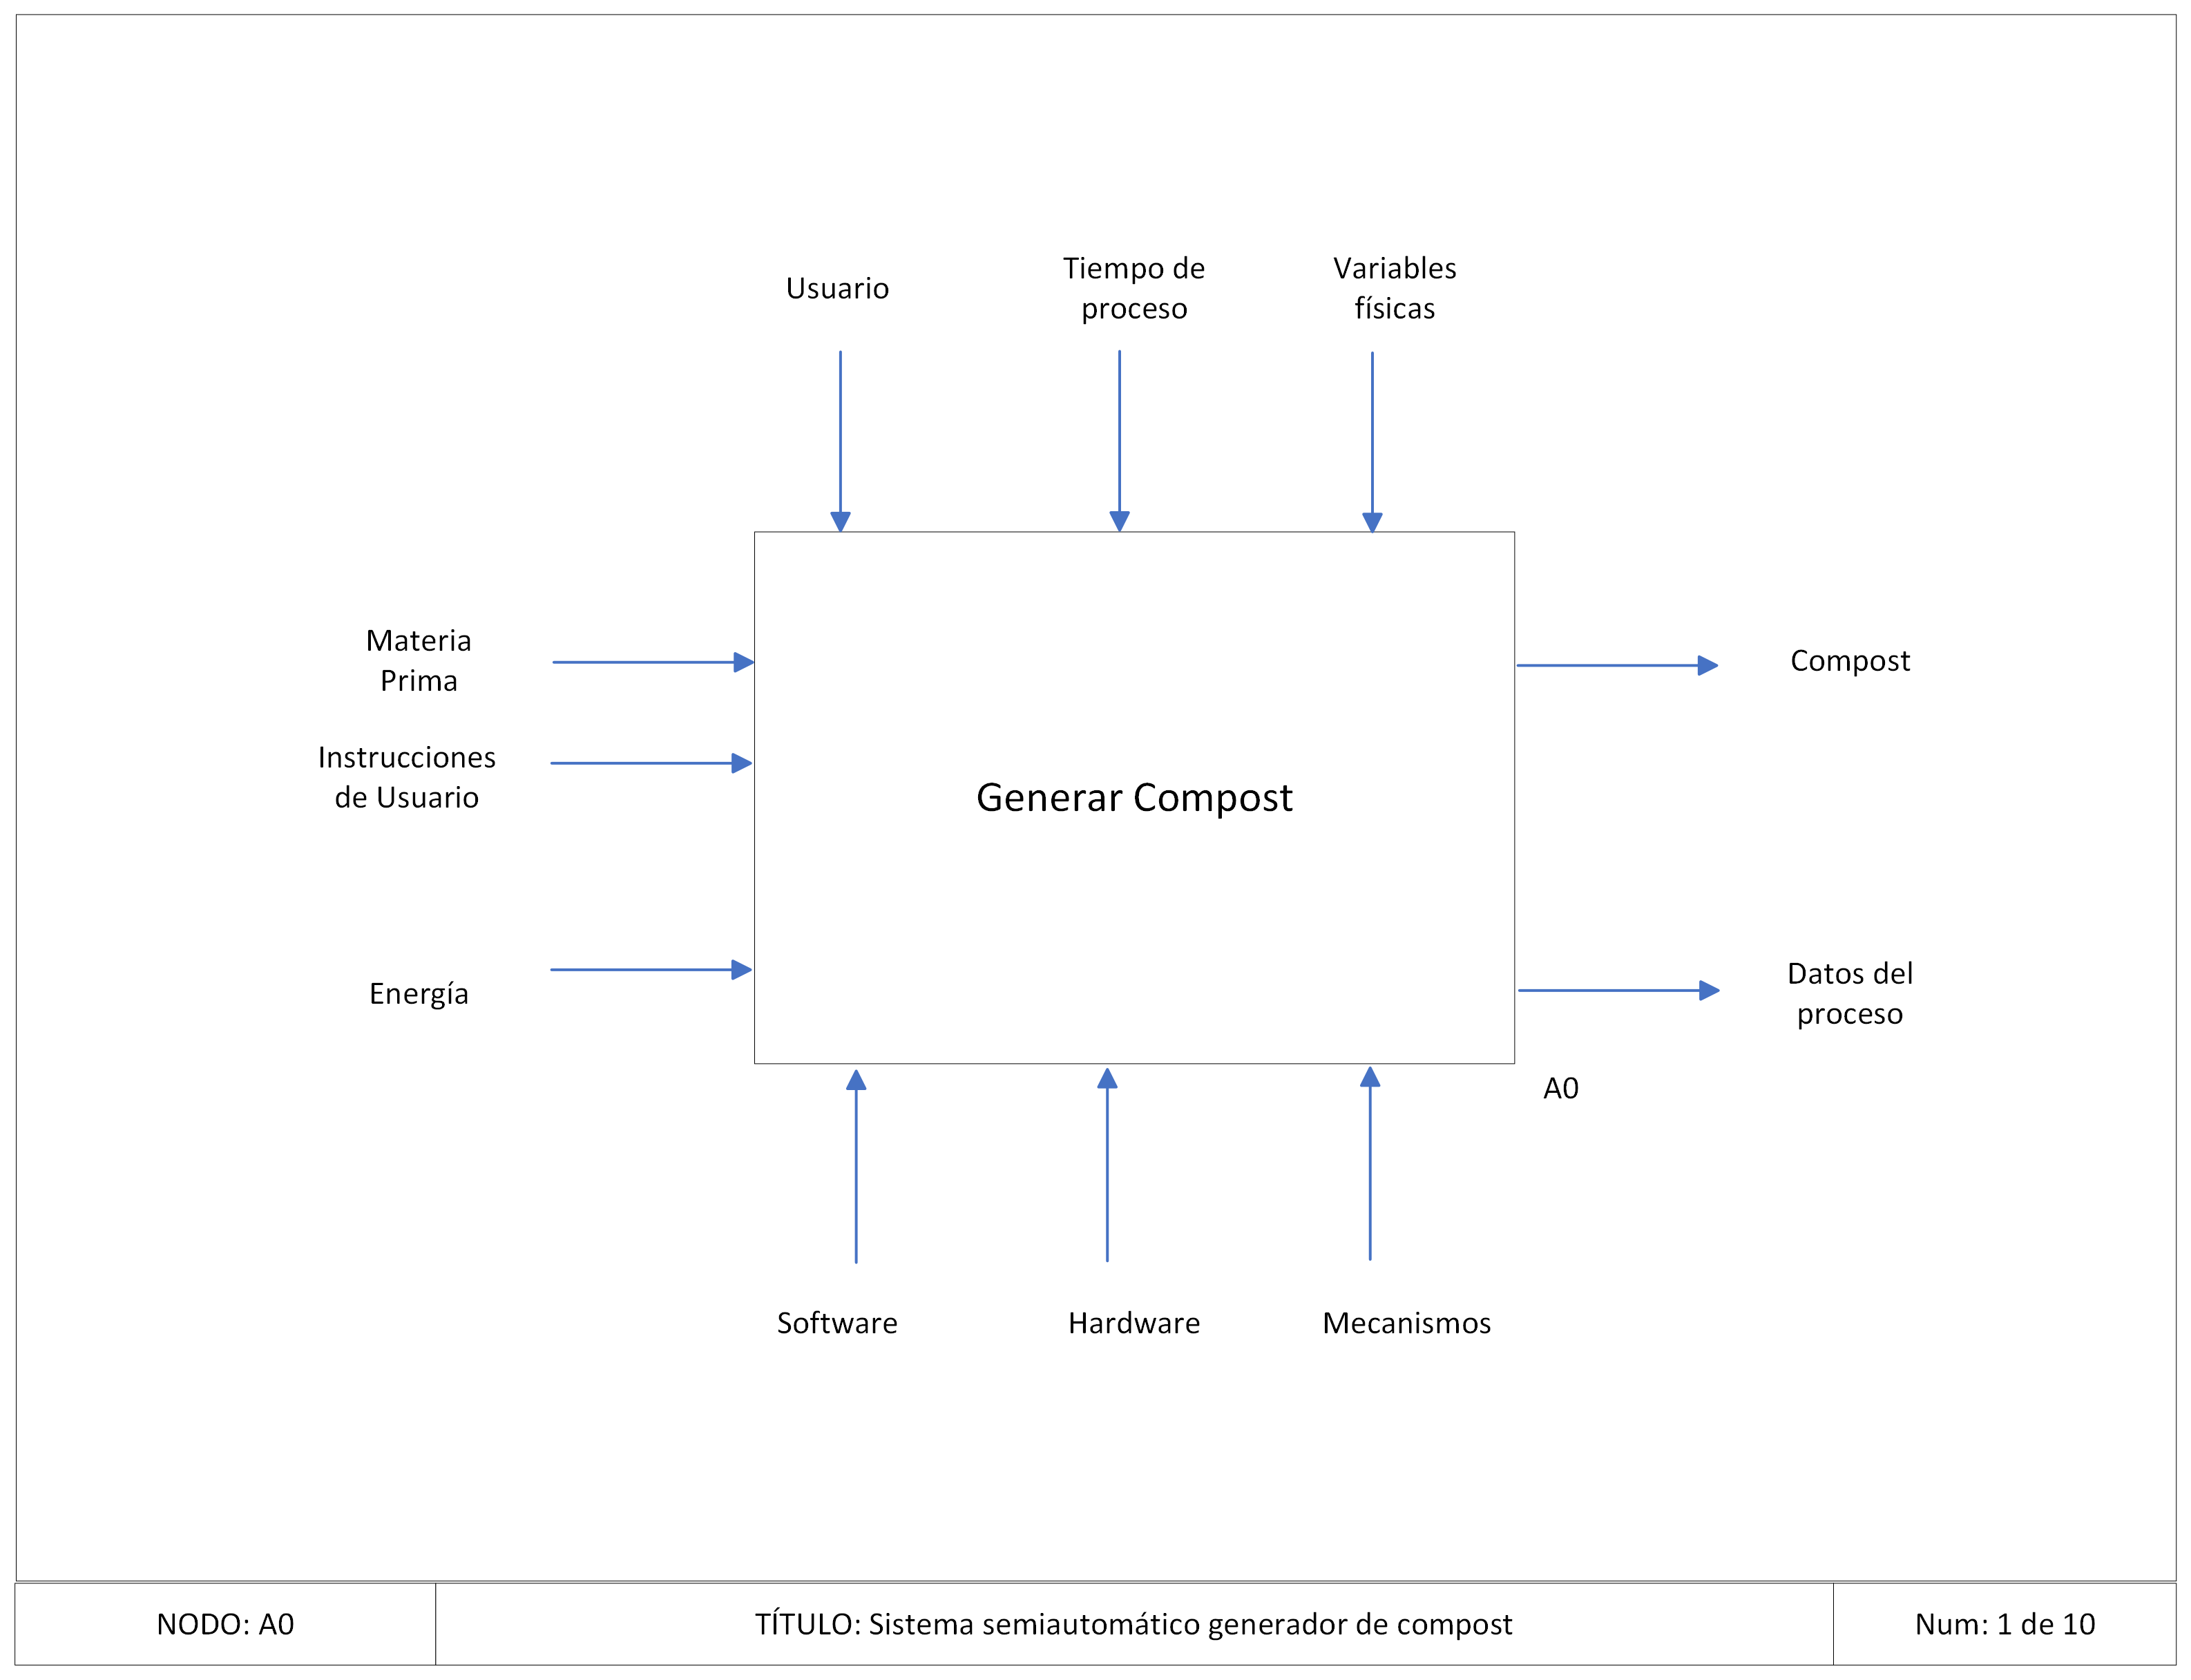
\includegraphics[scale=0.35, angle = 90]{images/Capitulo 6 Apéndices/01 IDEF 0/A0_final.png}
        \end{figure}
\newpage

\begin{figure}[h]
            \centering
            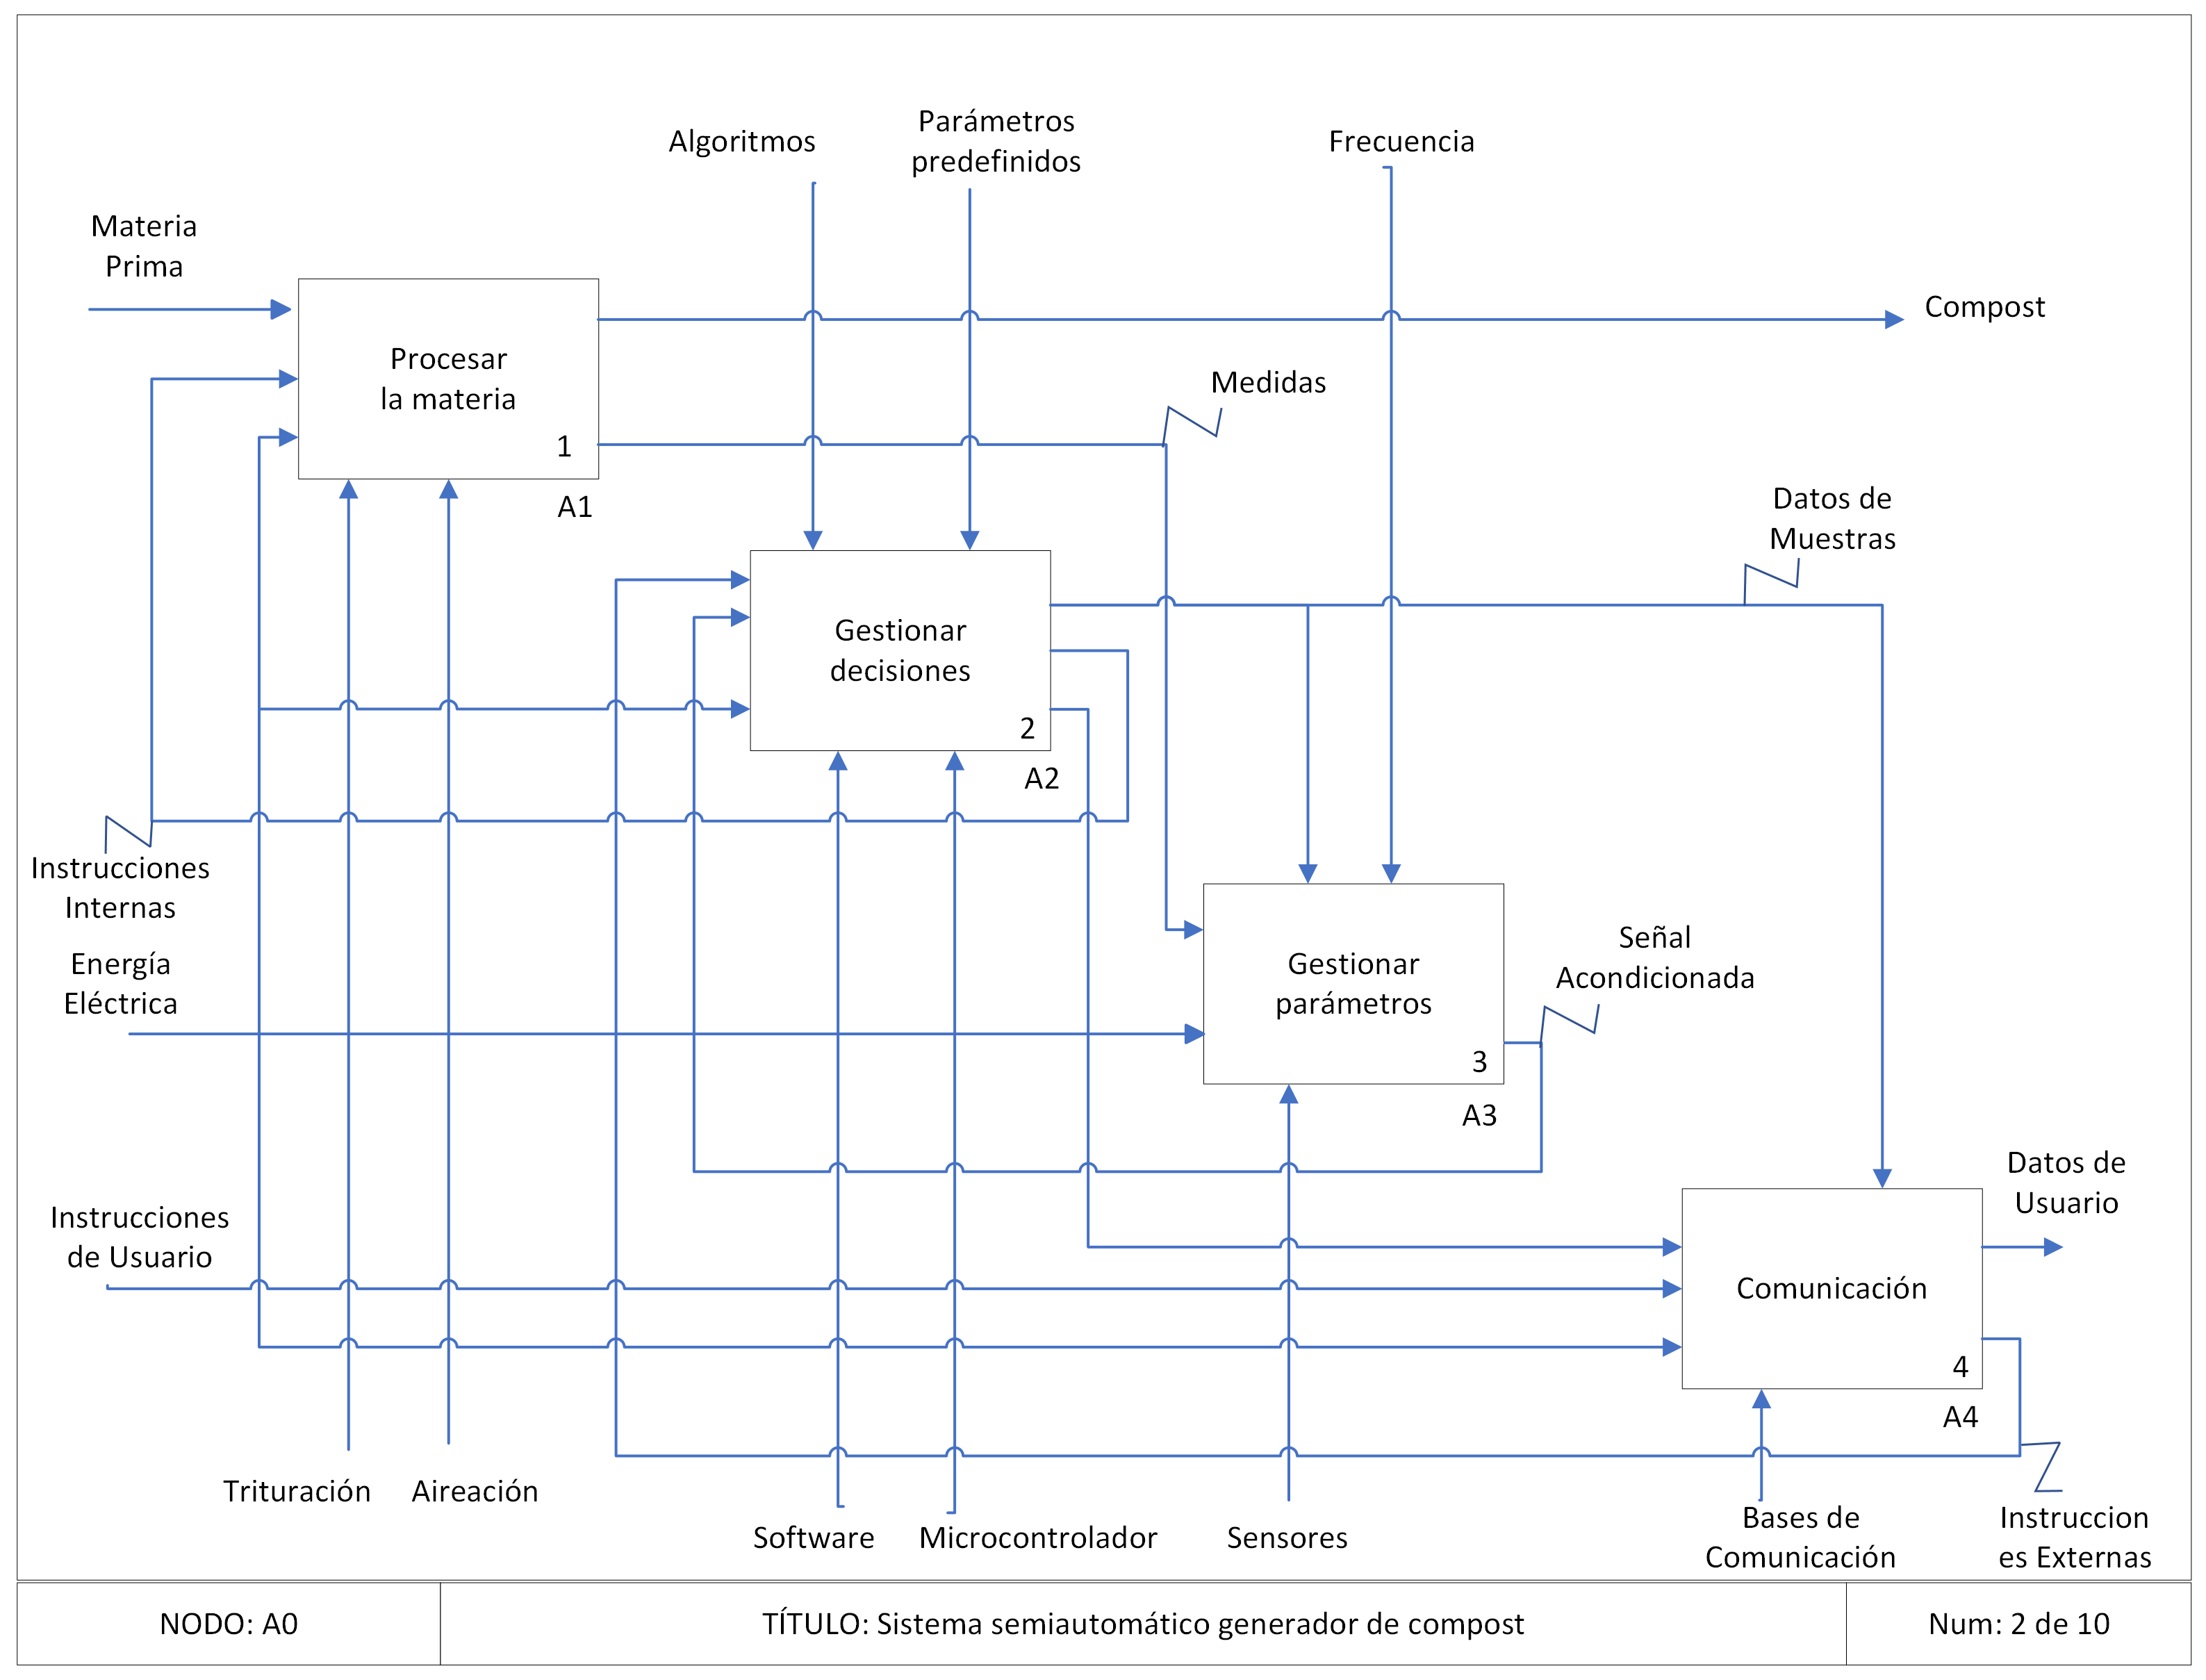
\includegraphics[scale=0.35, angle = 90]{images/Capitulo 6 Apéndices/01 IDEF 0/NodoA0.png}
        \end{figure}
\newpage

\begin{figure}[h]
            \centering
            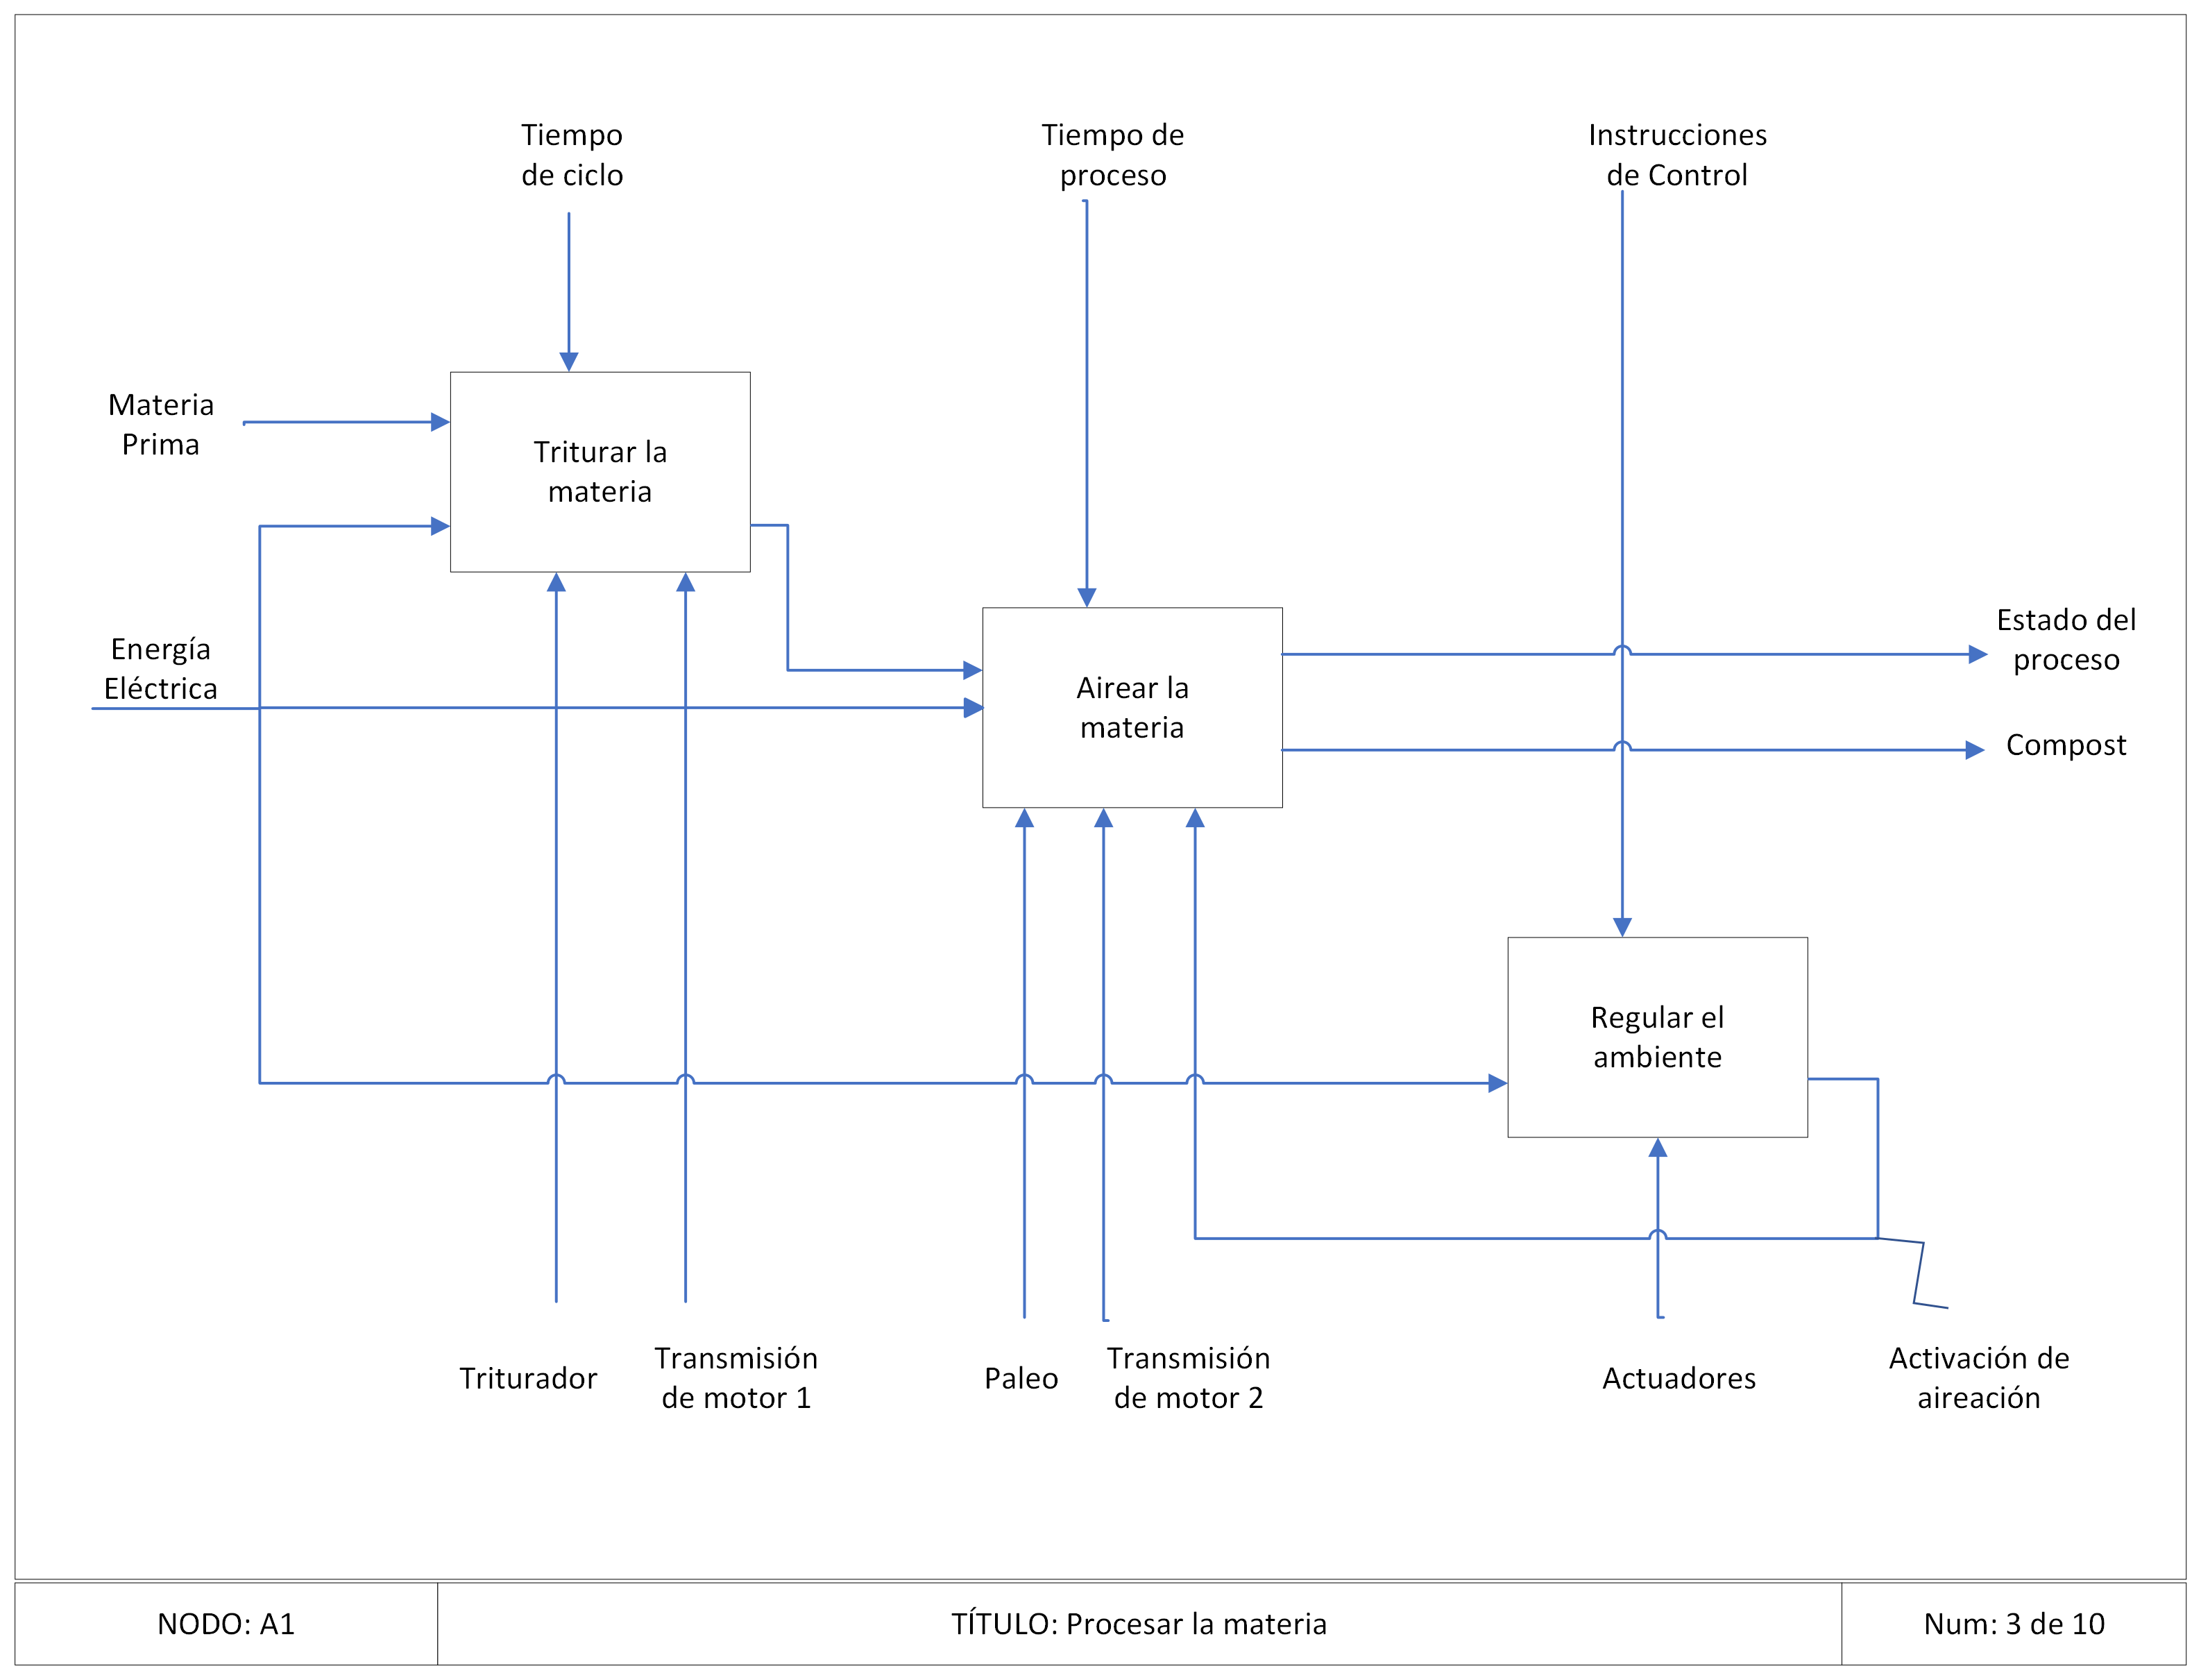
\includegraphics[scale=0.35, angle = 90]{images/Capitulo 6 Apéndices/01 IDEF 0/A1_final - Copy.png}
        \end{figure}
\newpage

\begin{figure}[h]
            \centering
            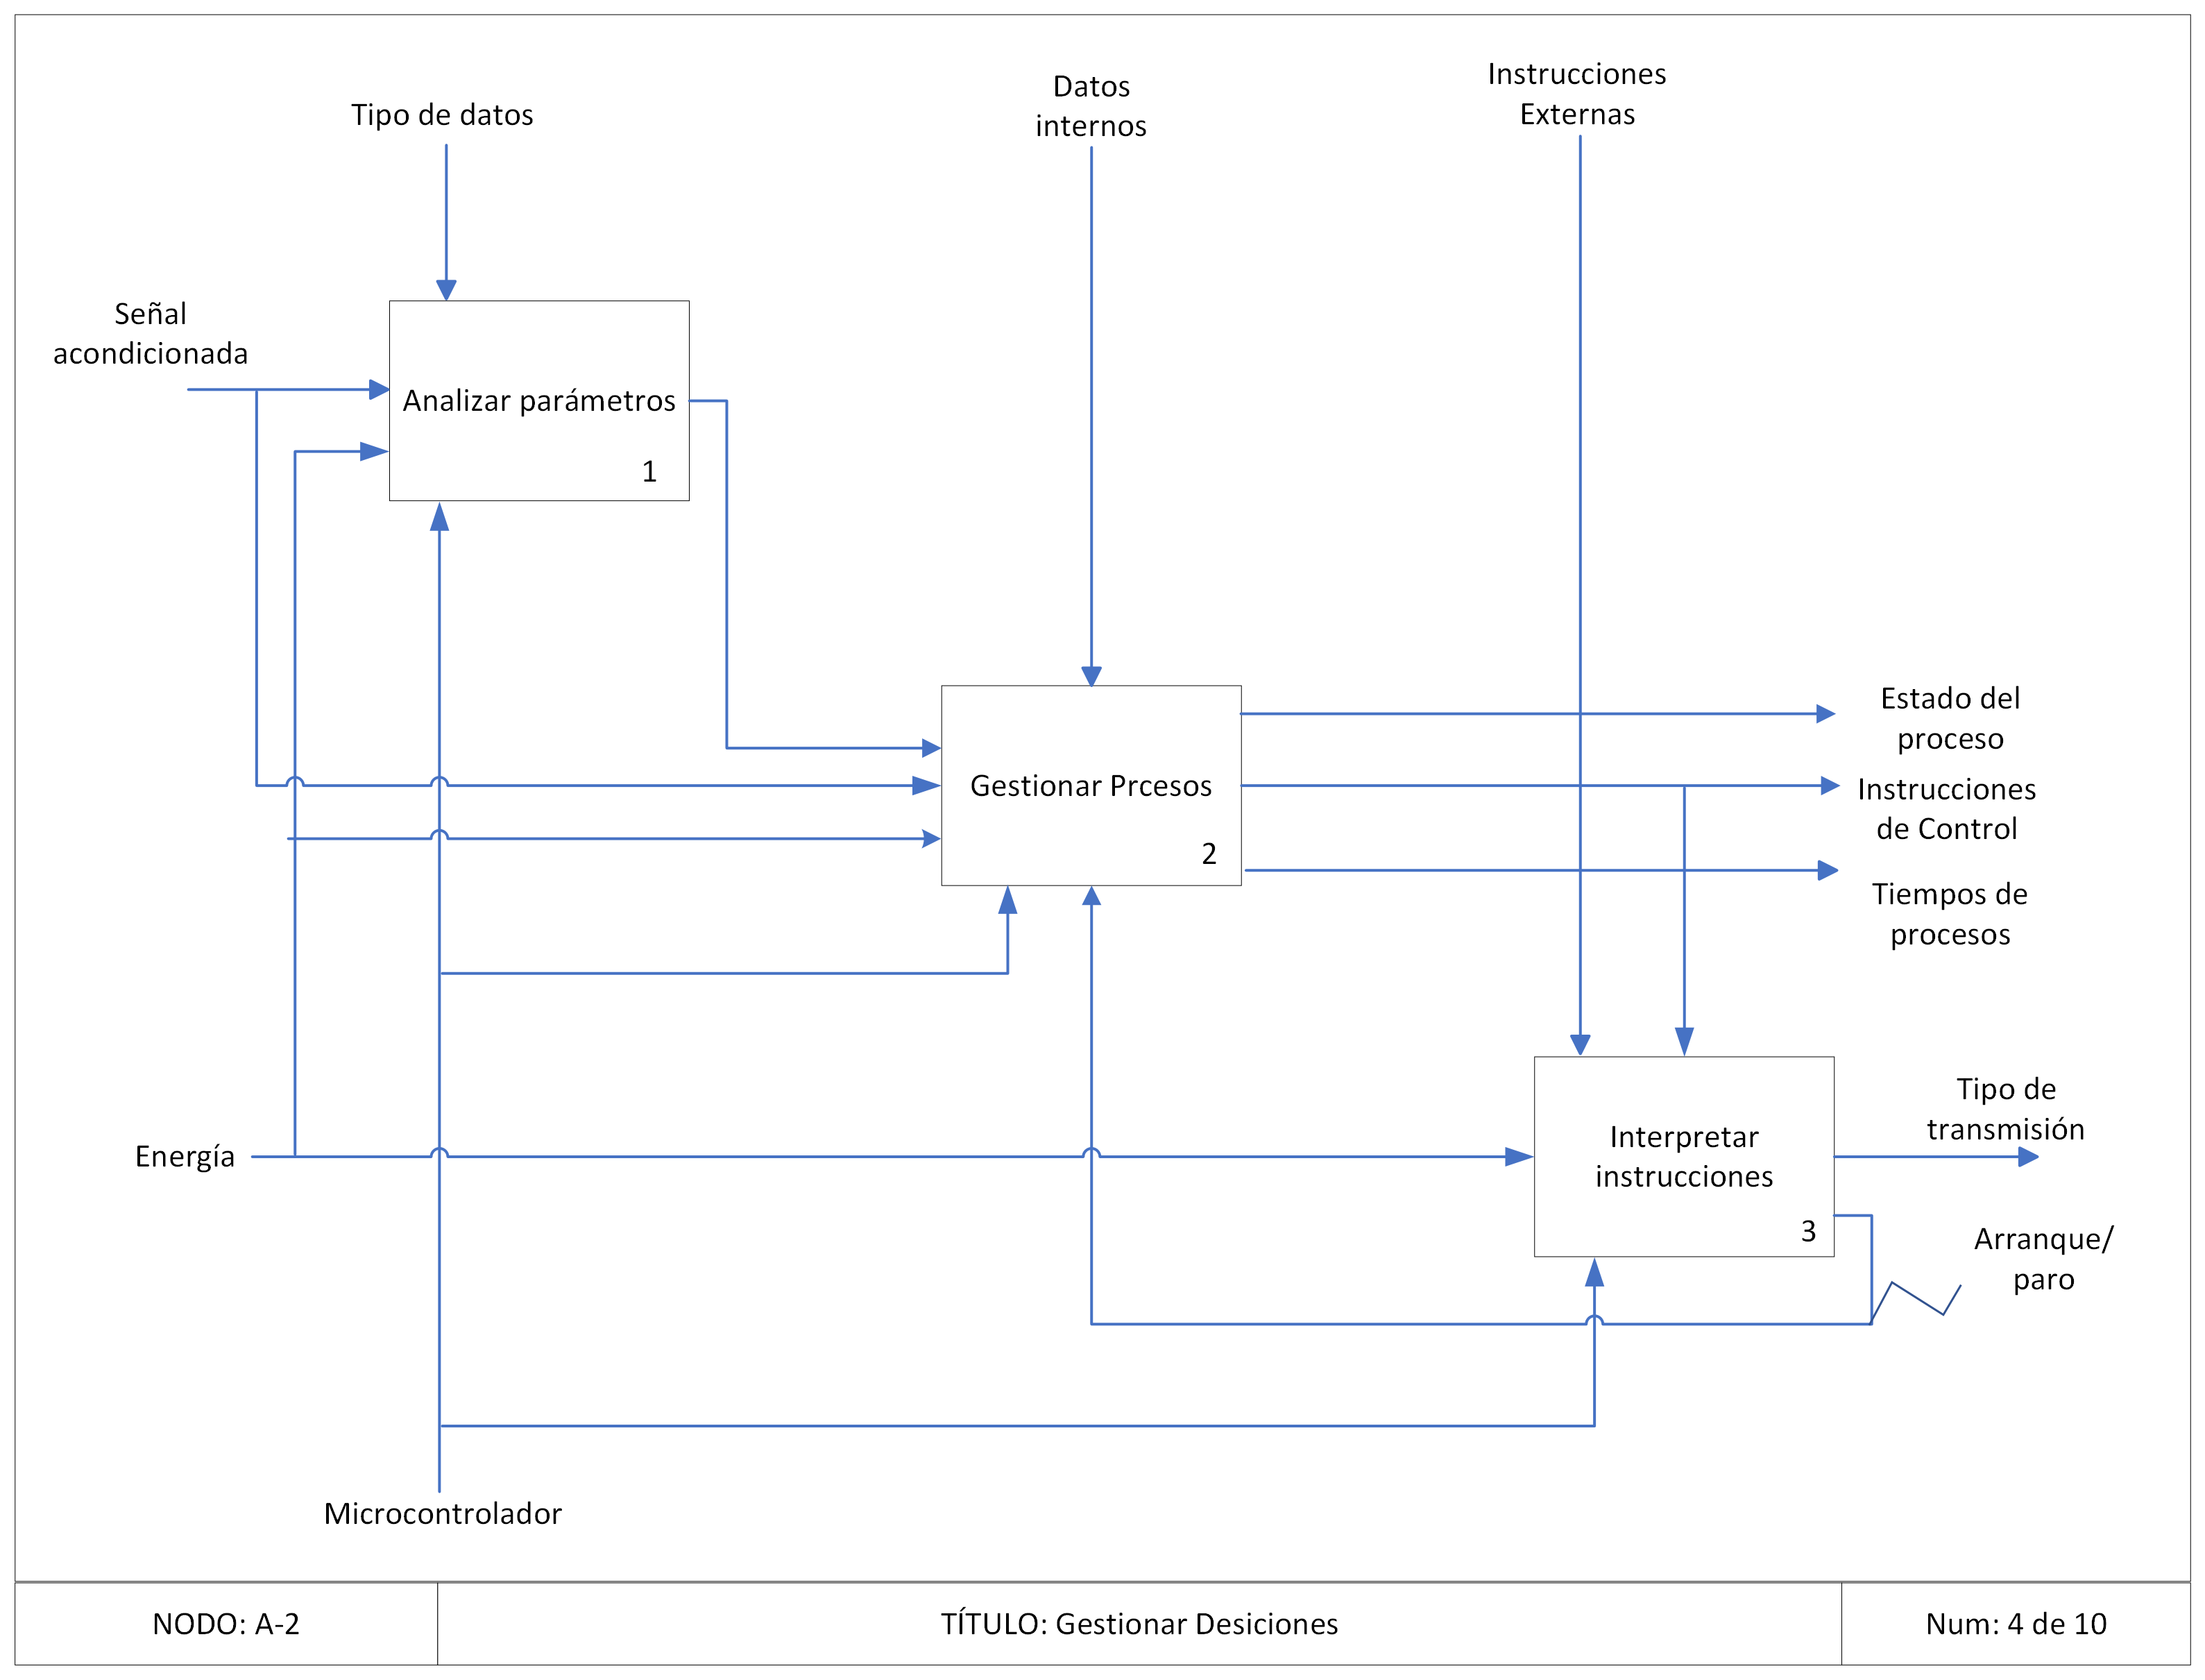
\includegraphics[scale=0.35, angle = 90]{images/Capitulo 6 Apéndices/01 IDEF 0/A2_conmarco - Copy.png}
        \end{figure}
\newpage

\begin{figure}[h]
            \centering
            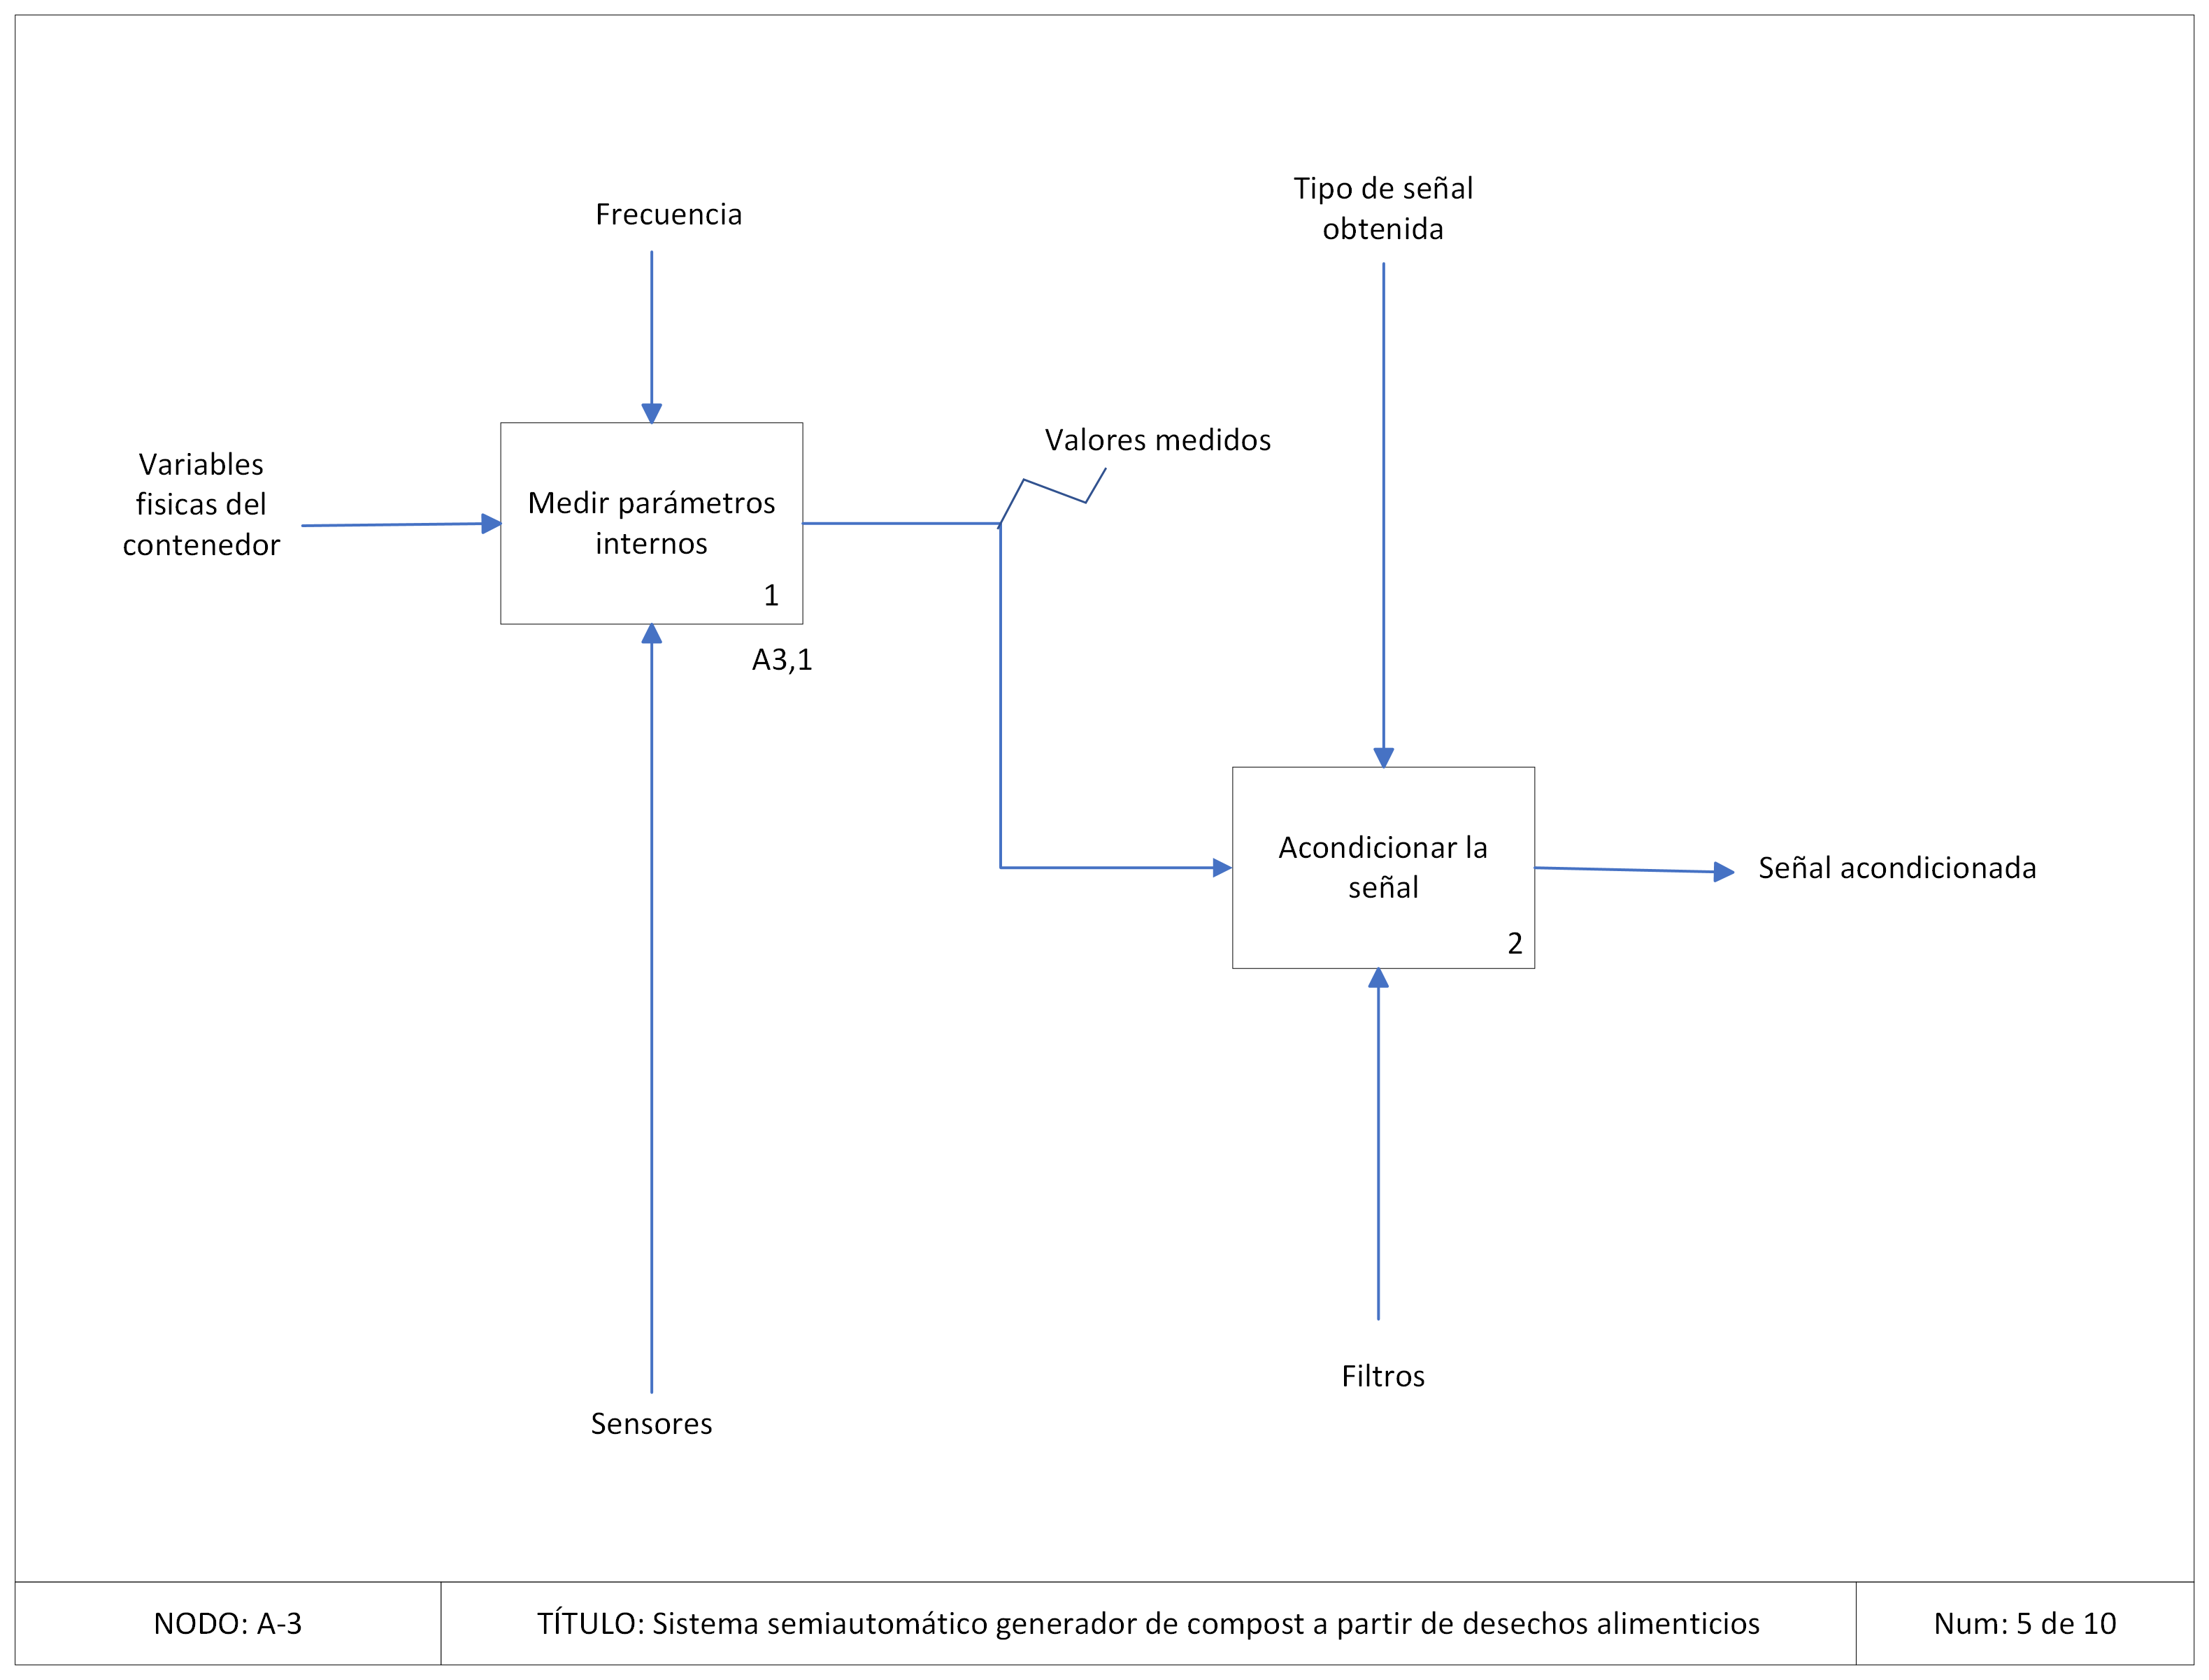
\includegraphics[scale=0.35, angle = 90]{images/Capitulo 6 Apéndices/01 IDEF 0/A3_conmarco - Copy.png}
        \end{figure}
\newpage

\begin{figure}[h]
            \centering
            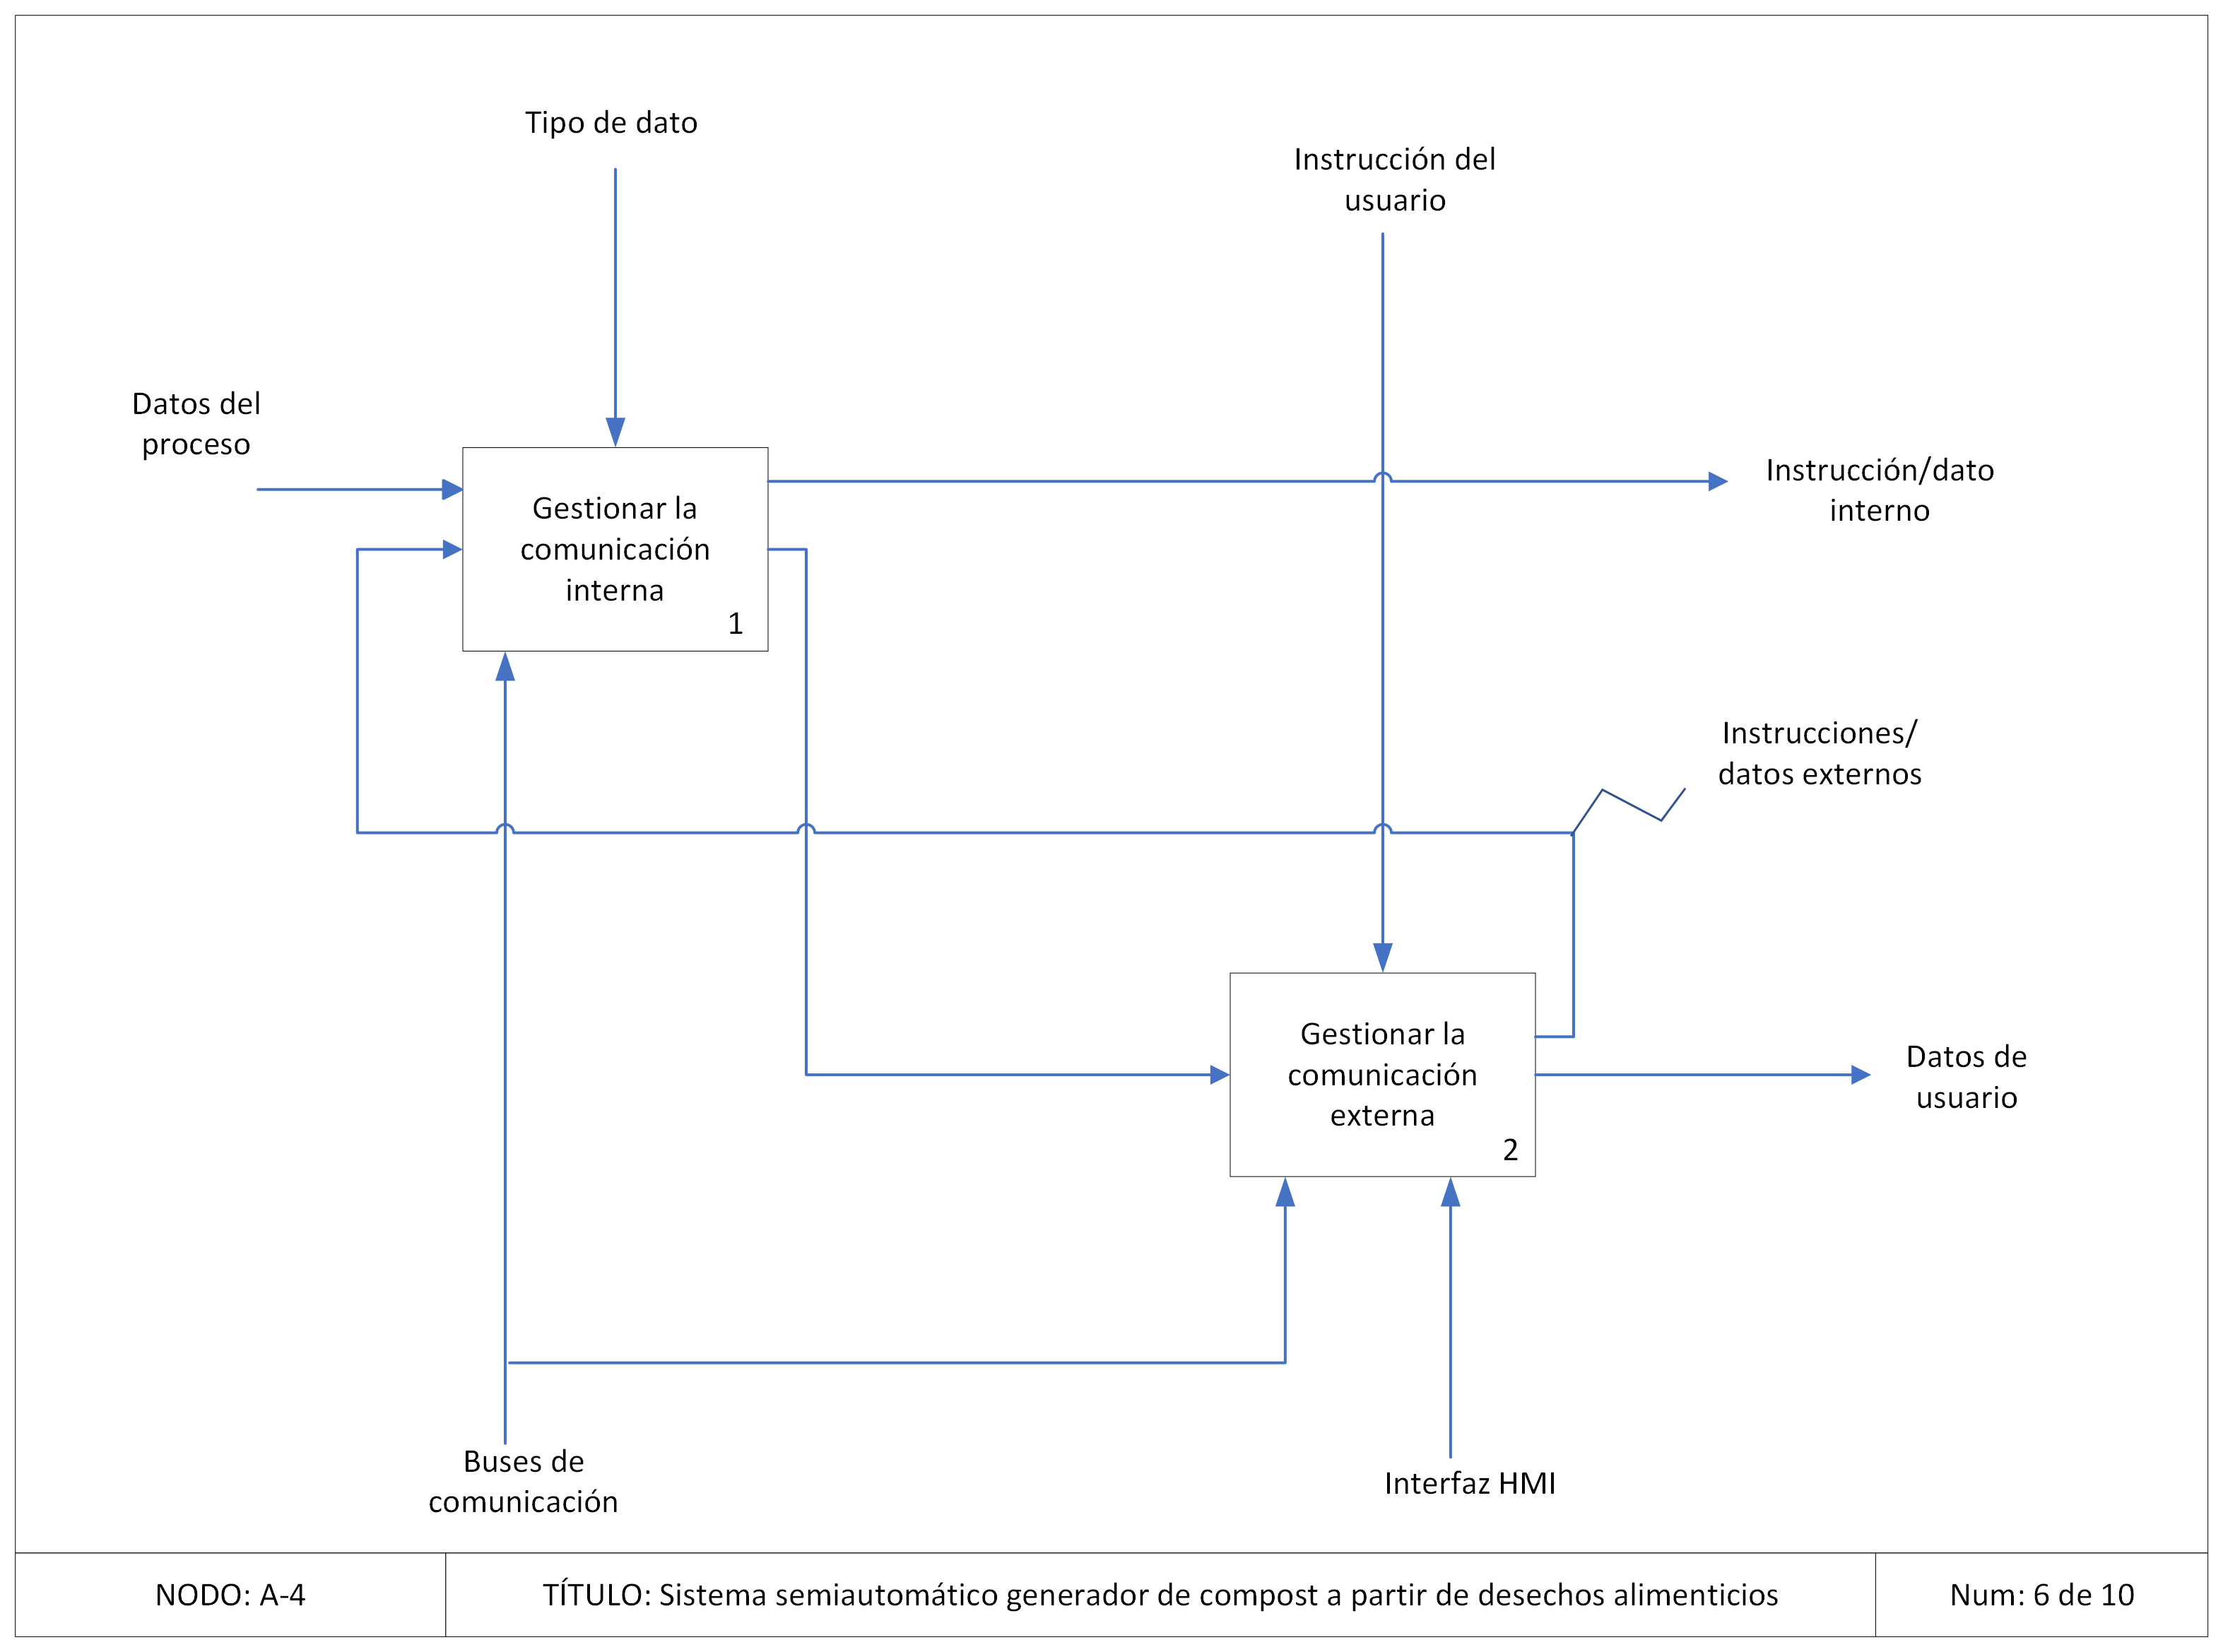
\includegraphics[scale=0.35, angle = 90]{images/Capitulo 6 Apéndices/01 IDEF 0/A4_conmarco - Copy.png}
        \end{figure}
\newpage

%\begin{figure}[h]
%            \centering
%            \includegraphics[scale=0.35, angle = 90]{images/Capitulo 6 Apéndices/01 IDEF 0/A5_conmarco - Copy.png}
%        \end{figure}
%\newpage

\begin{figure}[h]
            \centering
            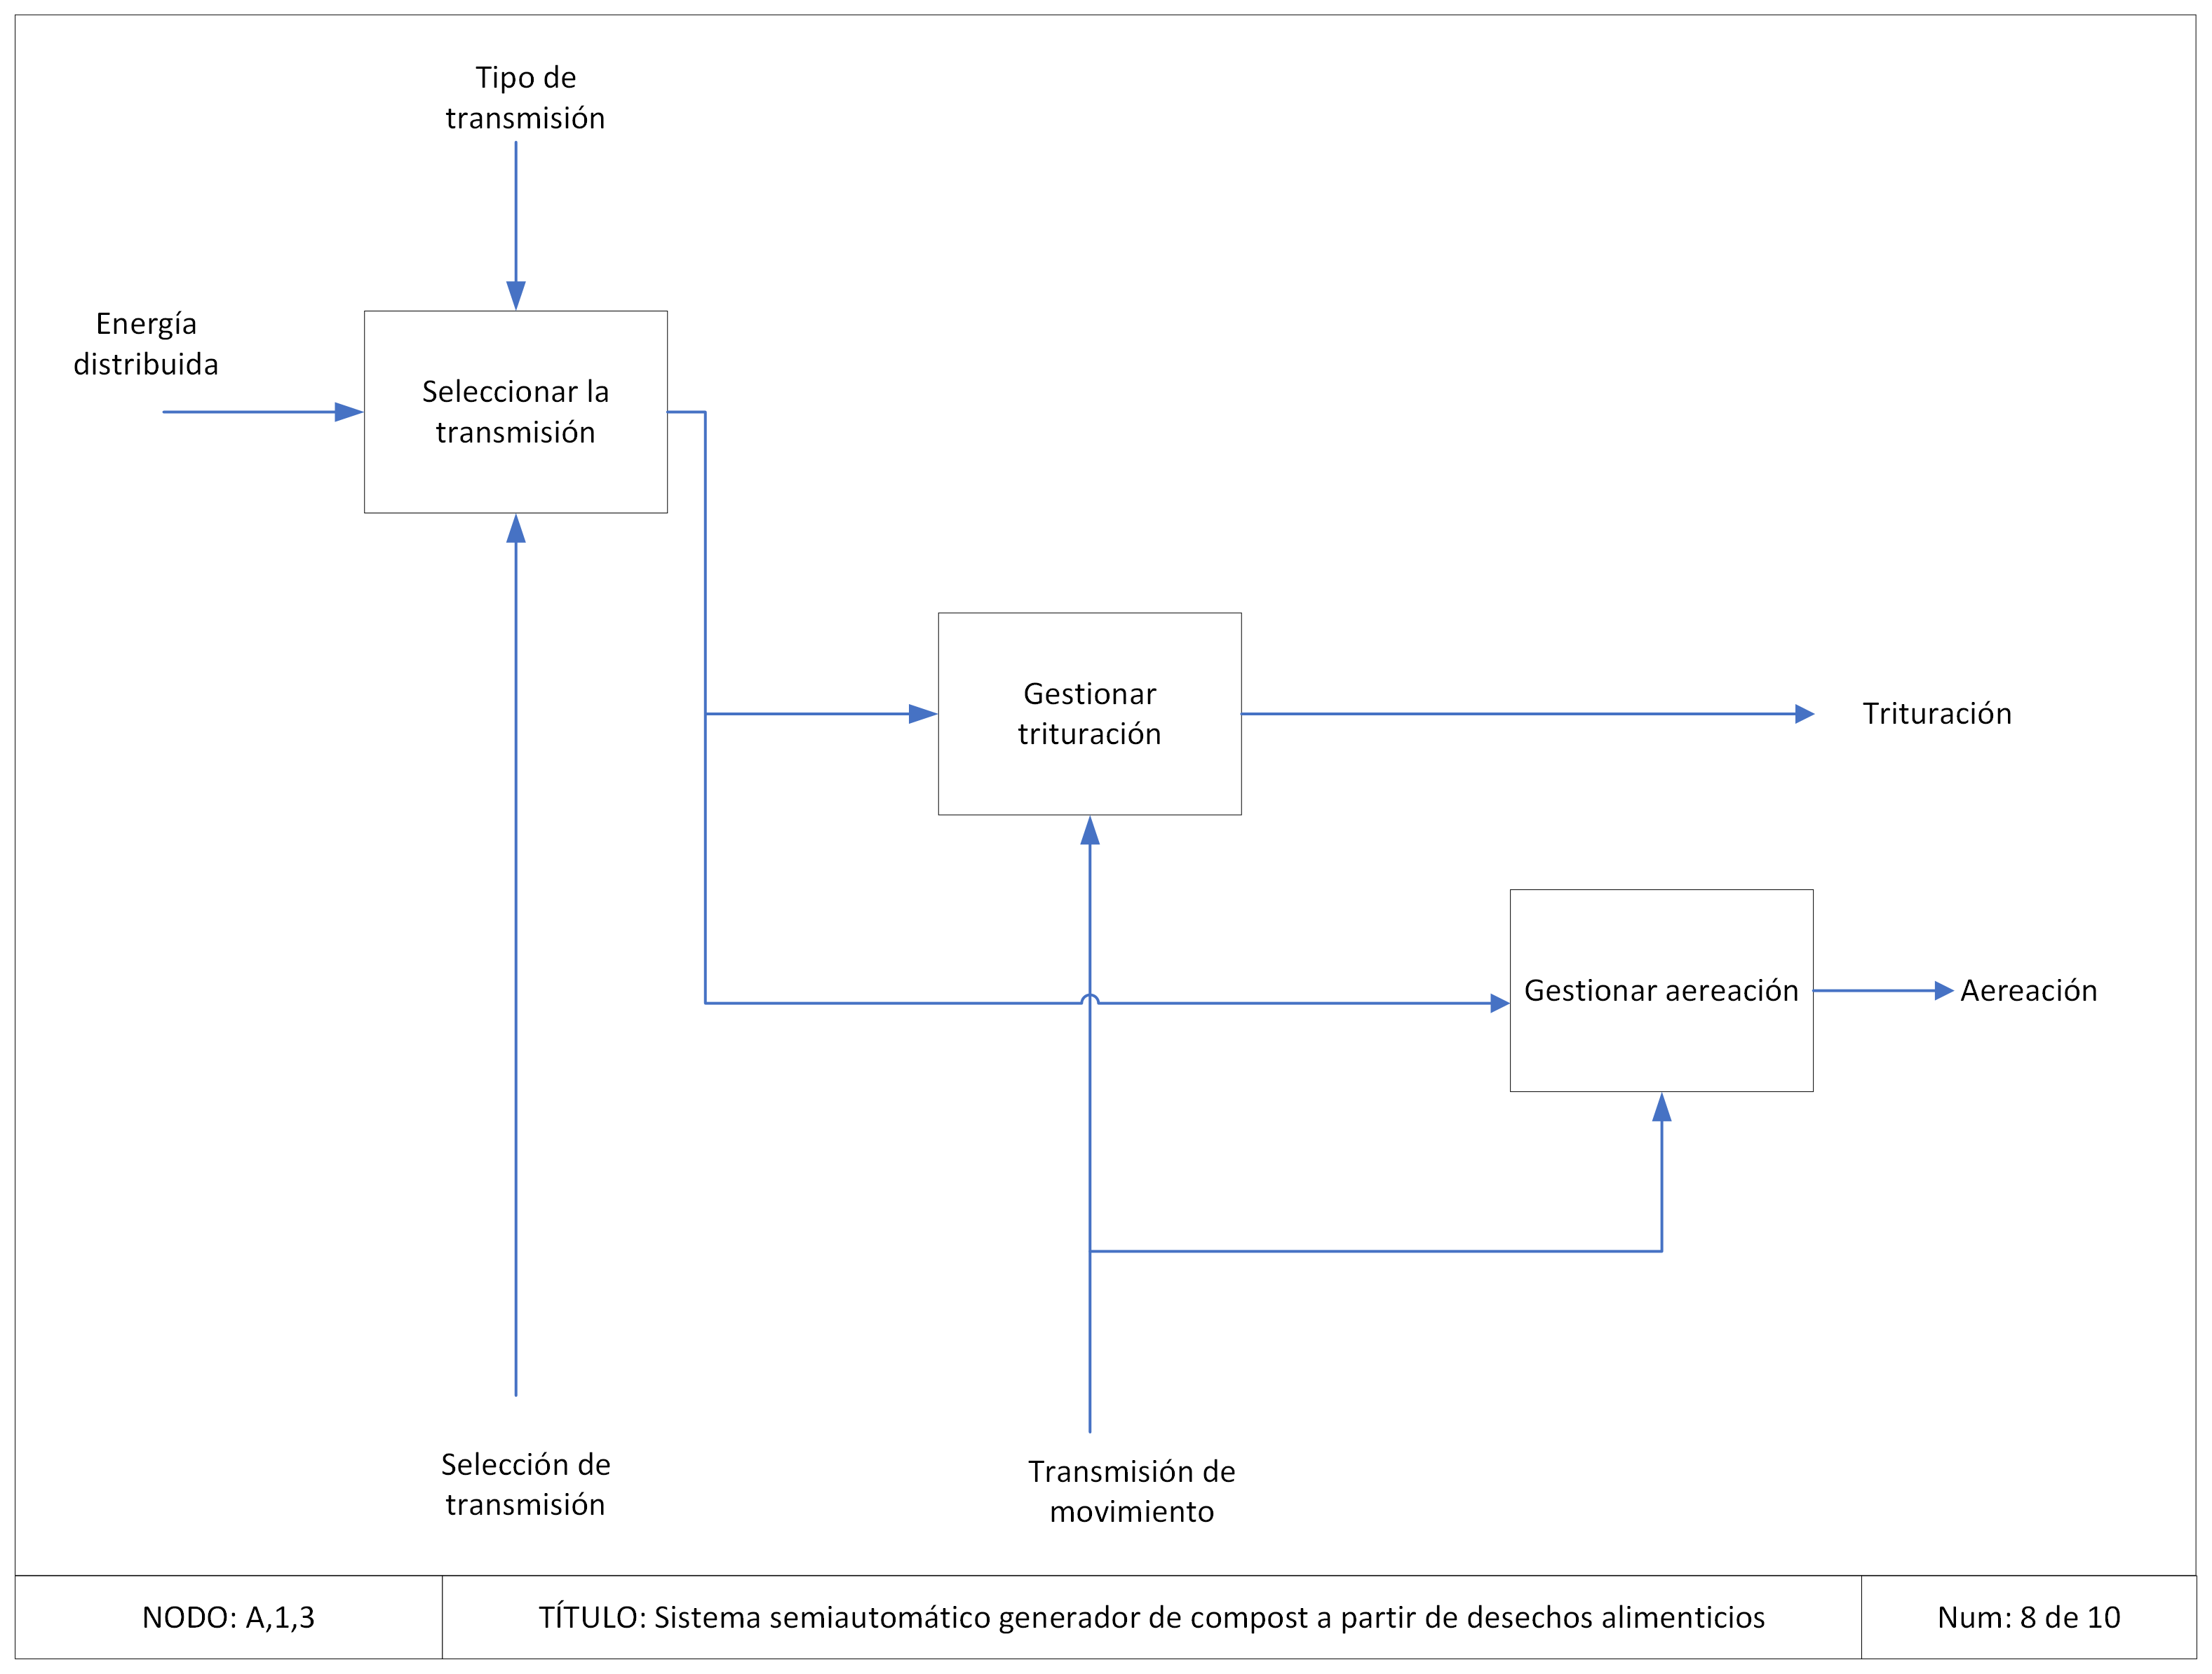
\includegraphics[scale=0.35, angle = 90]{images/Capitulo 6 Apéndices/01 IDEF 0/A,1,3_conmarco - Copy.png}
        \end{figure}
\newpage

\begin{figure}[h]
            \centering
            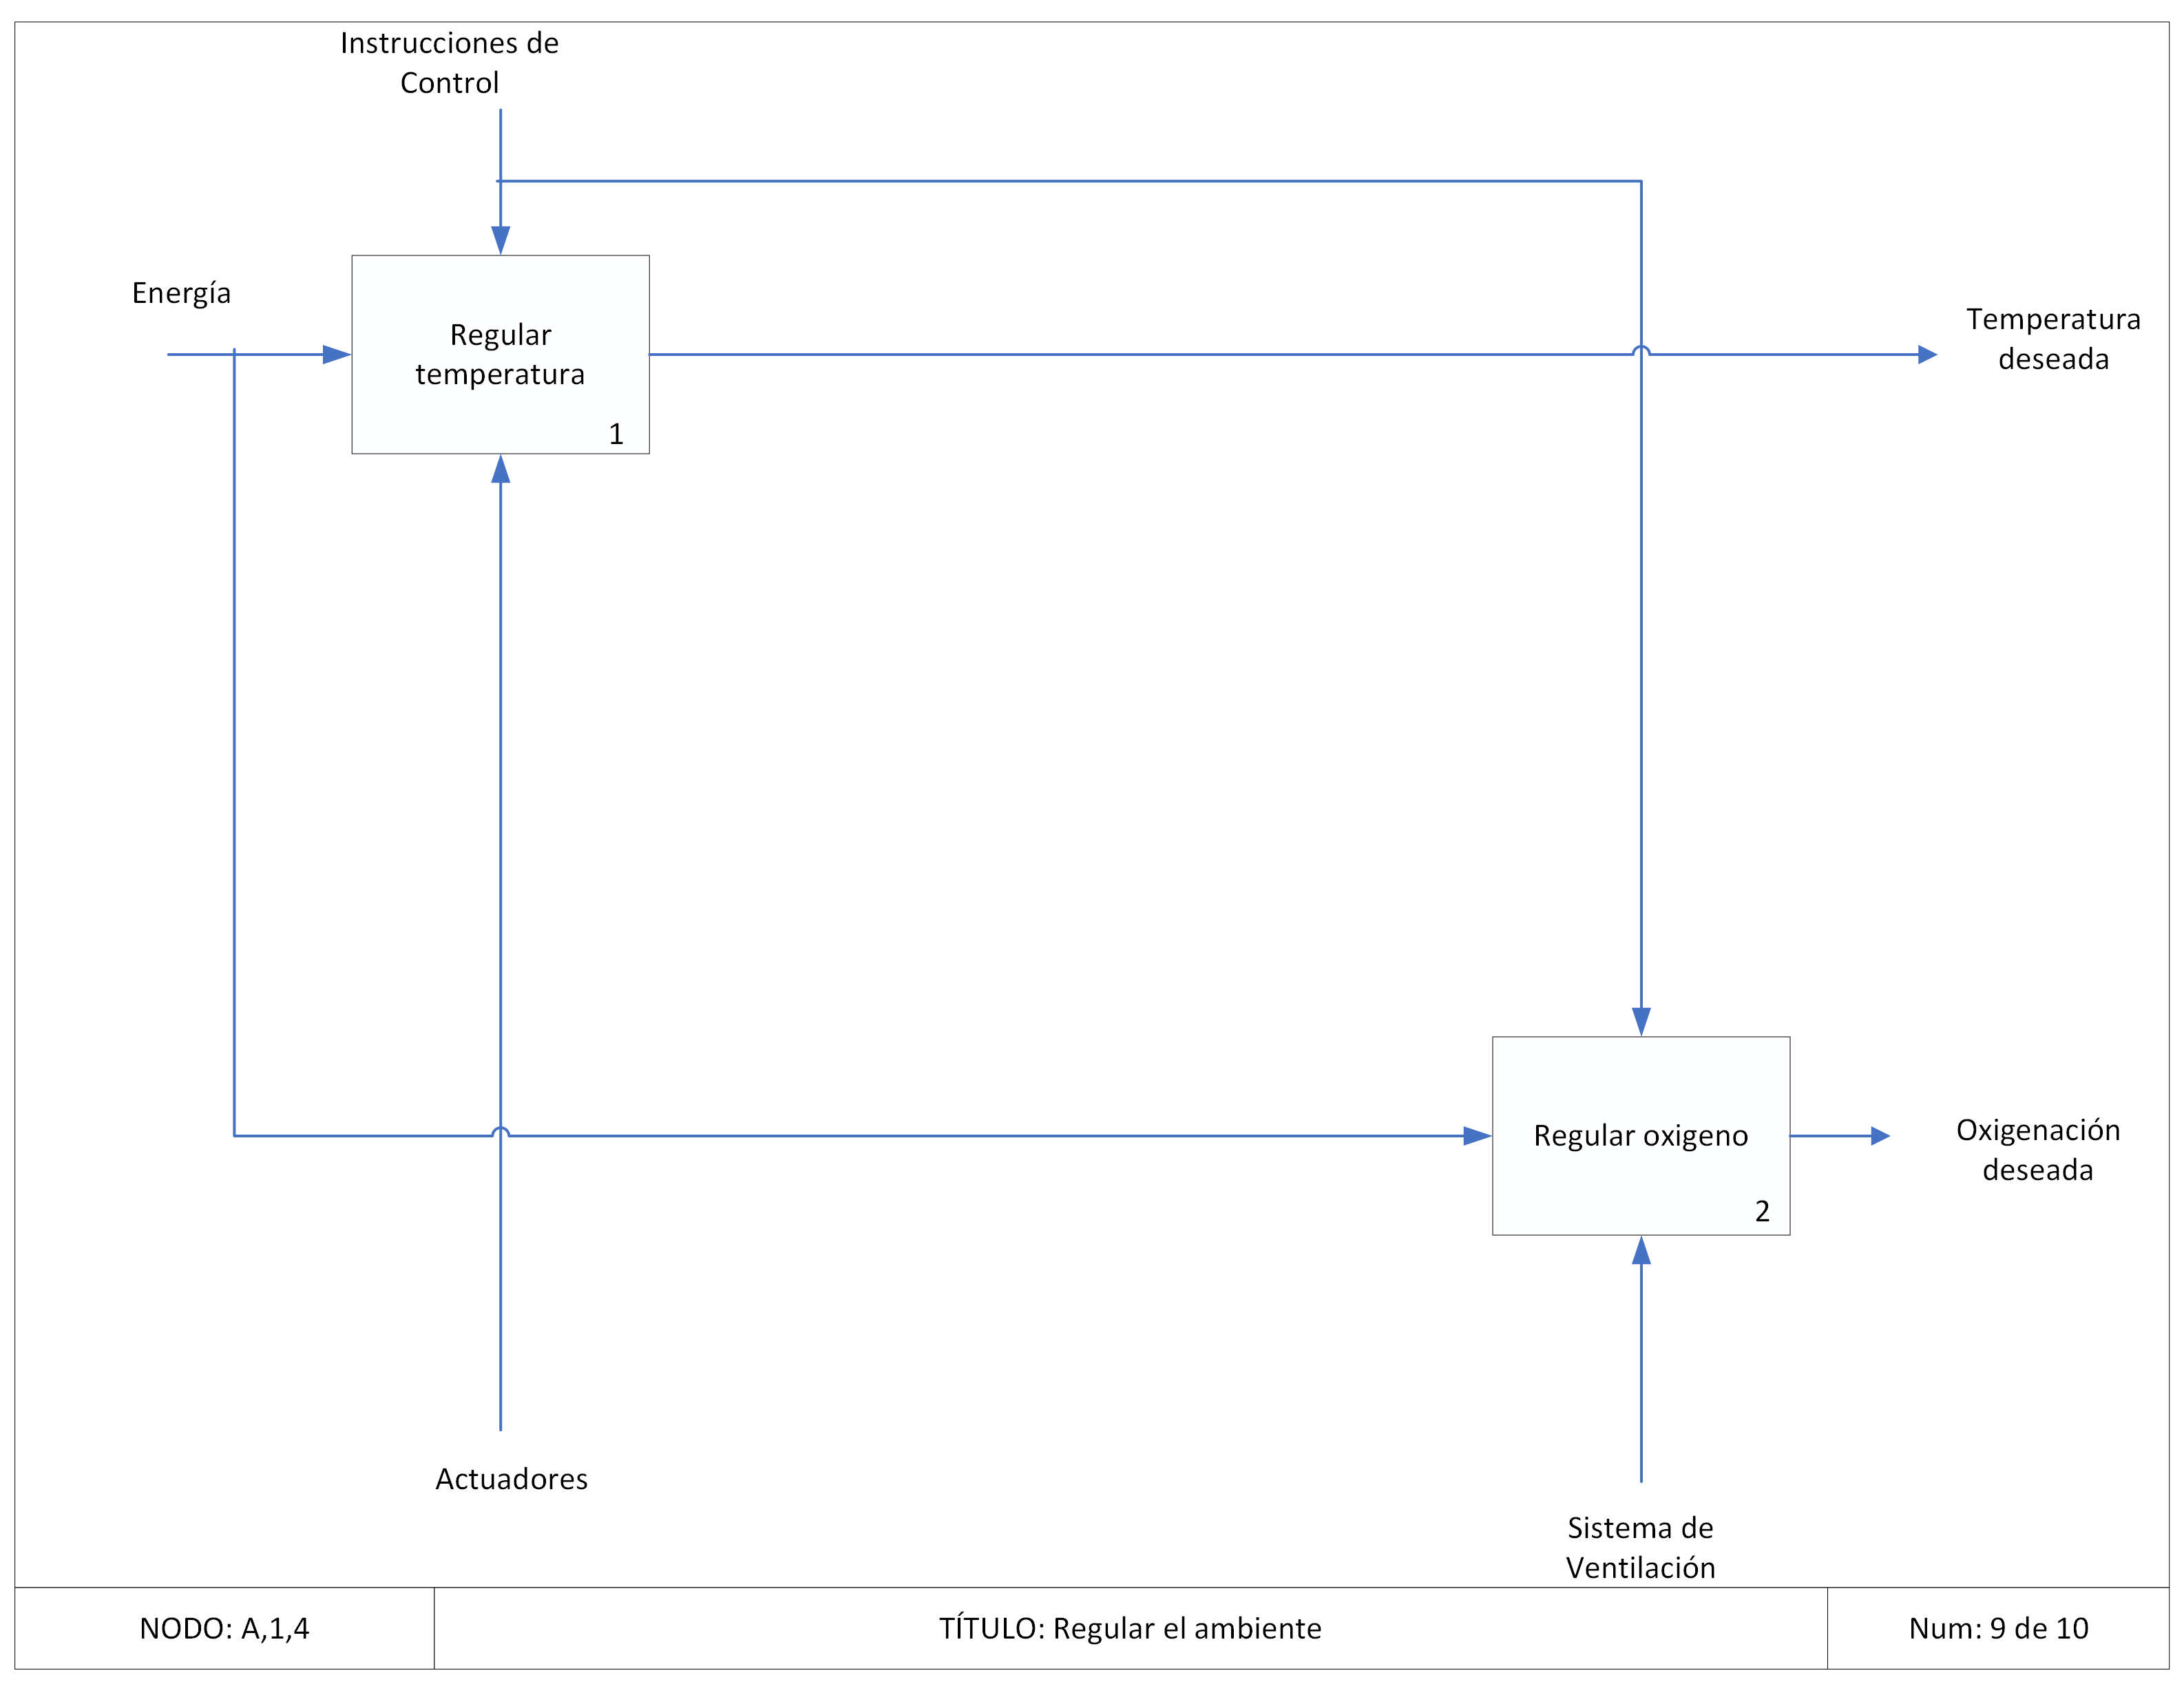
\includegraphics[scale=0.35, angle = 90]{images/Capitulo 6 Apéndices/01 IDEF 0/A,1,4_conmarco - Copy.png}
        \end{figure}
\newpage

\begin{figure}[h]
            \centering
            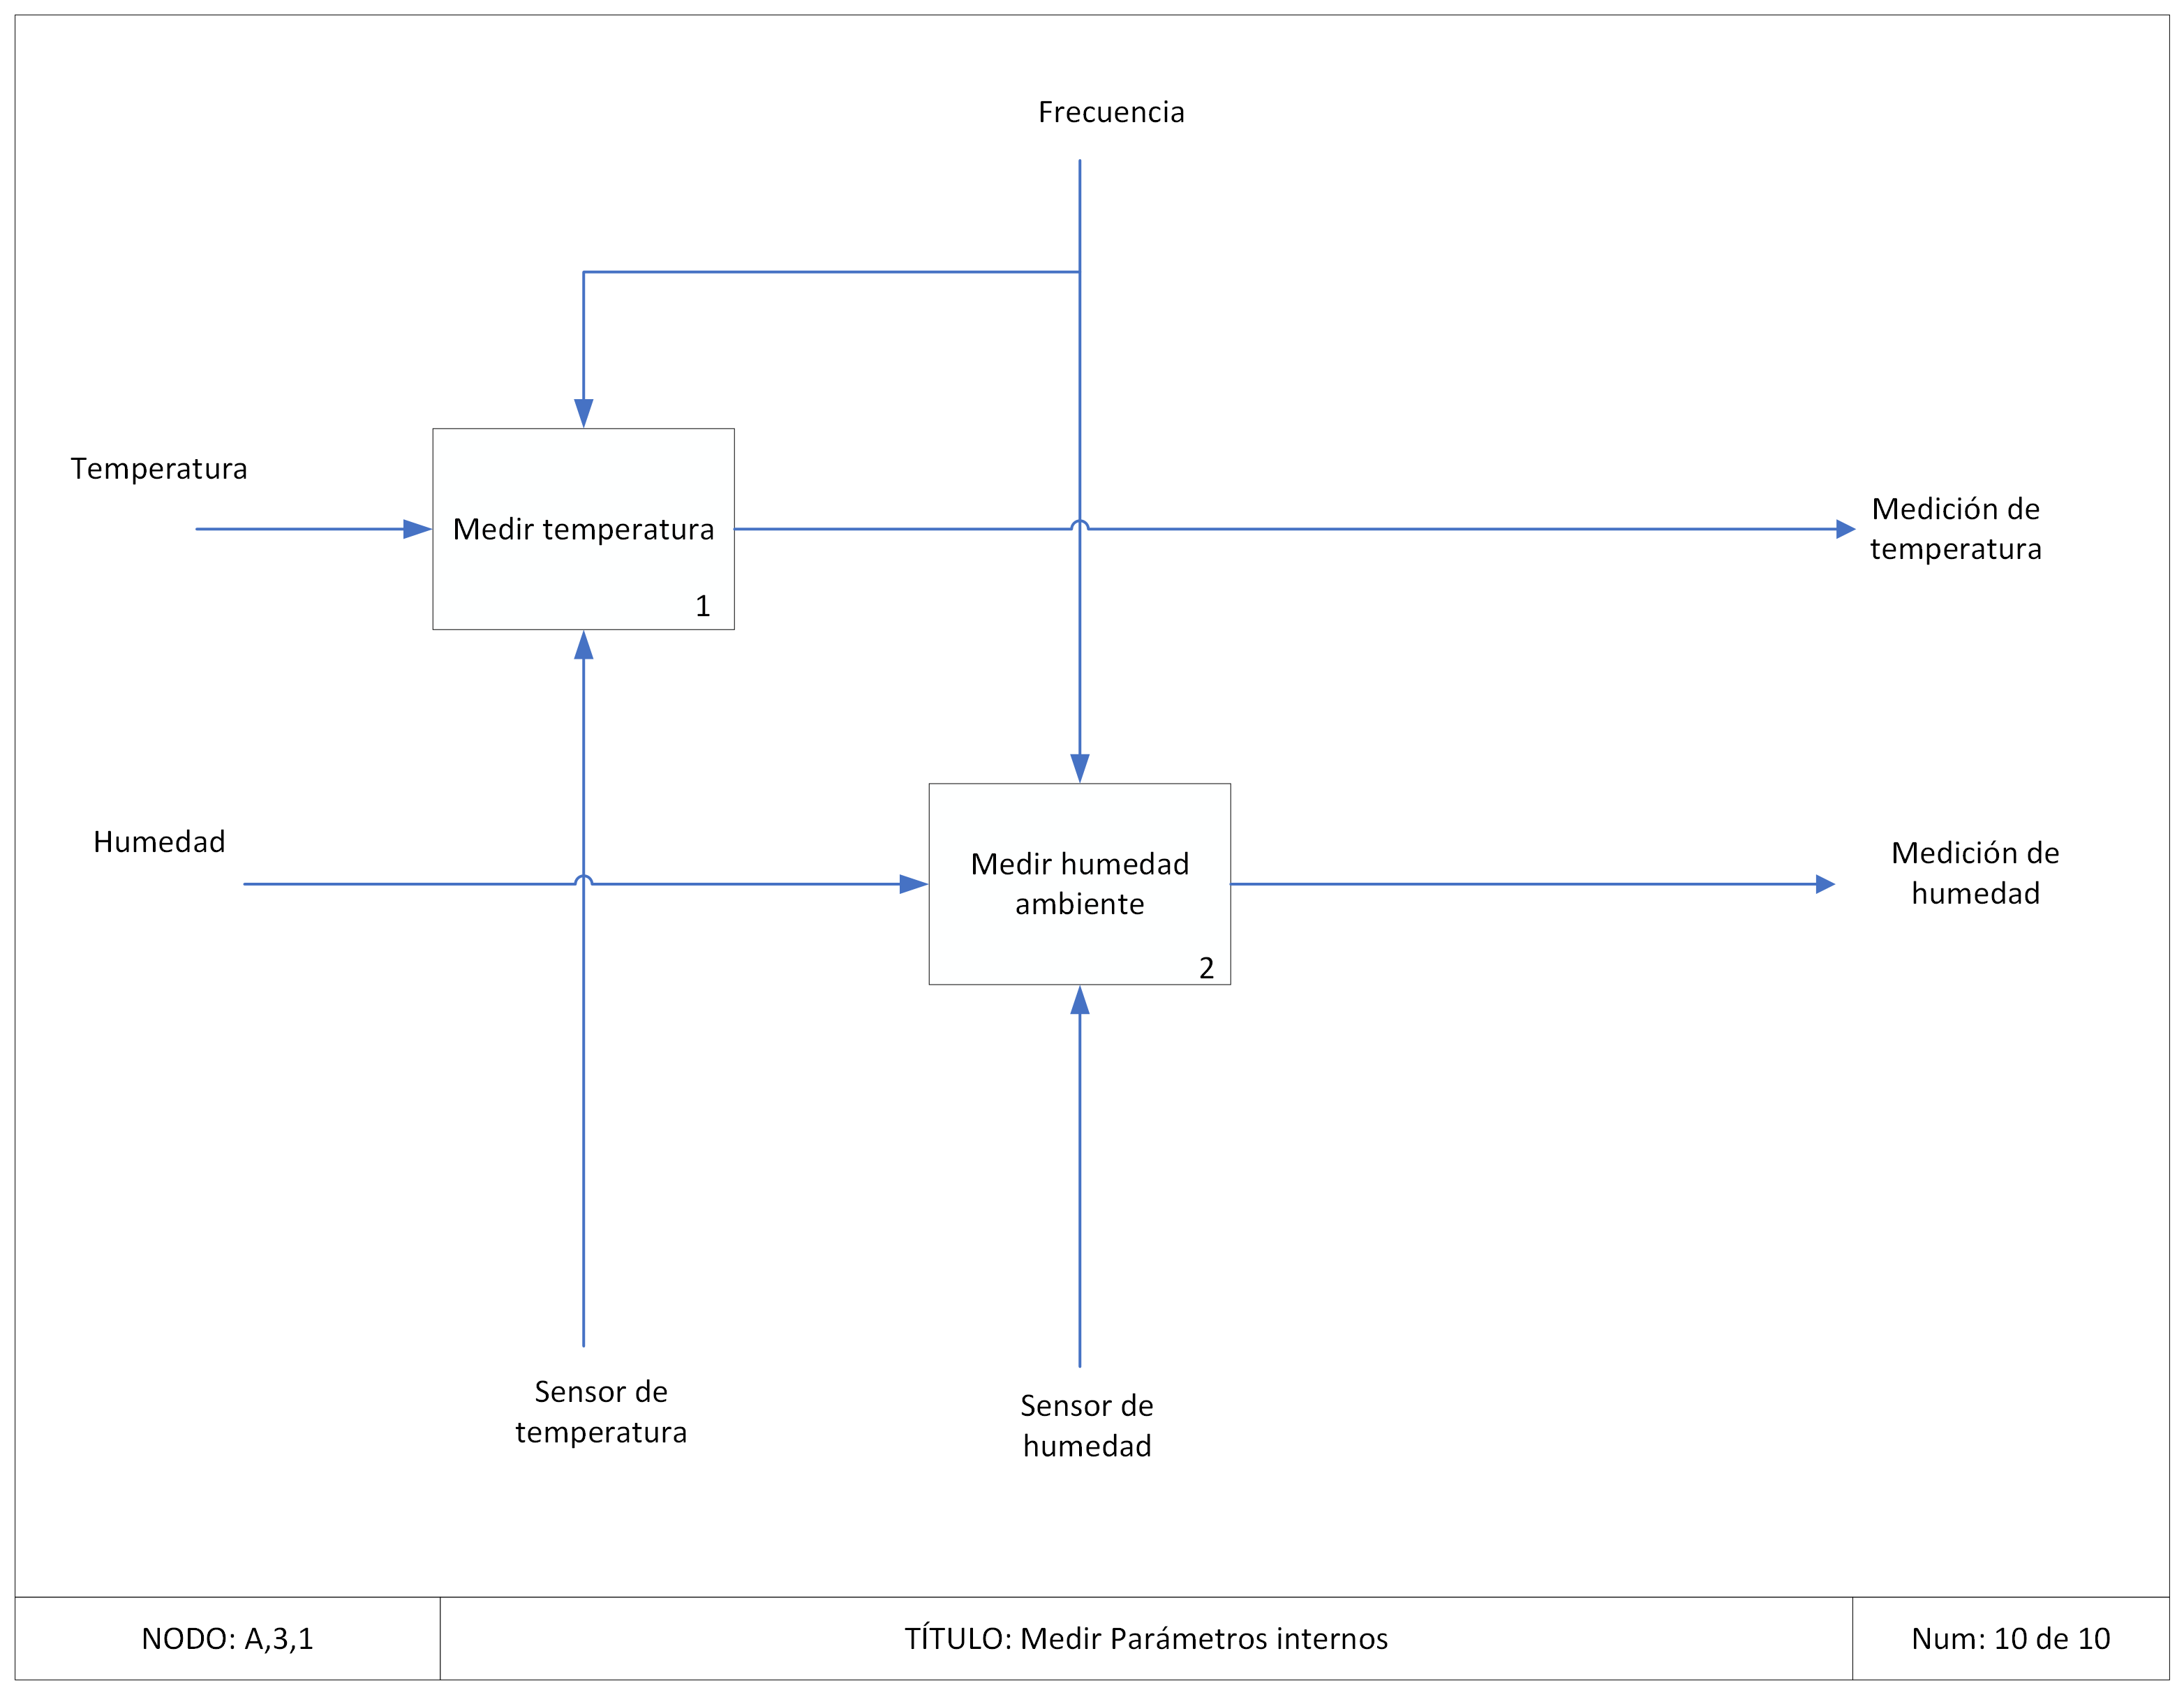
\includegraphics[scale=0.35, angle = 90]{images/Capitulo 6 Apéndices/01 IDEF 0/A,3,1_conmarco - Copy.png}
        \end{figure}
\newpage
%\include{apendices/apendices/7.2.2_Matriz_Morfologica}
%\section{Descripción de Criterios de Selección}\label{Ap:Crit}

Mediante el Proceso de Análisis Jerárquico (AHP), el cual es un método de selección multi-criterio se procedió a evaluar las distintas propuestas de solución que buscan solucionar todas las necesidades identificadas previamente.

Para poder realizar la selección de los diferentes componentes se consideraron una serie de criterios, los cuales son los siguientes:

\begin{itemize}
    \item Costo:
    Mientras el precio sea menor se le asigna una mayor calificación.
    \item Facilidad de manufactura:
    Se refiere a que tan fácil es manufacturar, en caso de ser necesario, el componente a utiliza.
    \item Disponibilidad:
    Es la facilidad con la que es posible conseguir algún componente en el mercado.
    \item Seguridad de uso:
    Representa el riesgo que puede presentar para una persona determinado sistema o componente, mientras más peligroso menor ponderación obtiene.
    \item Facilidad de uso:
    Mientras más sencillo sea de utilizar por personas sin los conocimientos técnicos, mejor evaluación.
    \item Integración:
    Hace referencia a la facilidad de interconectar un componente con otro, se busca tener un alto nivel de integración de un componente con otro.
    \item Durabilidad:
    Se refiera la tiempo de vida útil de cada componente.
    \item Mantenimiento:
    Facilidad con la cual pueda realizarse el mantenimiento de cierto componente, mientras más fácil mejor calificación.
    \item Ergonomía:
    Se trata de la relación y comodidad que se genera al utilizar algún componente, se busca una alta ergonomía.
    \item Portabilidad:
    Facilidad de desplazar un componente de un lugar a otro, se busca una alta portabilidad.
    \item Estética
    Agrado visual que genera cierto componente, sin tener en cuenta su funcionabilidad.
\end{itemize}

Estos diferentes criterios fueron ponderados, utilizando el criterio AHP, en una tabla, como se muestra en el apéndice \ref{Ap:Crit}, para determinar qué características son las más sobresalientes y que tendrán mayor peso al momento de realizar la selección de los elementos del sistema mecatrónico.

Aquí se hace la presentación de los valores utilizados para la evaluación de las diferentes soluciones tecnológicas propuestas, para elegir las mejores opciones.

\begin{table}
    \centering
    \caption{Cuantificación de los criterios}
    \resizebox{!}{20cm}{
    \begin{turn}{90}
      \begin{tabular}{|m{1.5cm}|c|m{1.5cm}|m{1.5cm}|m{1.5cm}|m{1.5cm}|m{1.5cm}|m{1.5cm}|m{1.5cm}|m{1.5cm}|m{1.5cm}|m{1.5cm}|m{1.5cm}|c|c|} \hline 
         Criterio&  &  Costo&  Facilidad de manufactura&  Disponi- bilidad&  Seguridad de uso&  Facilidad de uso&  Integra- cion&  Durabili- dad&    Manteni- miento&Ergono- mia&Portabi- lidad&Estetica  &Suma&Porcentaje\\ \hline 
         Costo&  1& \cellcolor[rgb]{ 1,  1,  0} X&  1&  1&  2&  2&  2&  2&    2&2&2&  2&18&16.7 \%\\ \hline 
         Facilidad de manufactura&  2&  1& \cellcolor[rgb]{ 1,  1,  0} X&  2&  2&  1&  1&  2&    2&2&2&  2&17&15.7 \%\\ \hline 
         Disponi- bilidad&  3&  1&  0& \cellcolor[rgb]{ 1,  1,  0} X&  1&  1&  2&  2&    2&2&2&  2&15&13.9 \%\\ \hline 
         Seguridad de uso&  4&  0&  0&  1& \cellcolor[rgb]{ 1,  1,  0} X&  2&  2&  2&    2&2&2&  2&15&13.9 \%\\ \hline 
         Facilidad de uso&  5&  0&  1&  1&  0& \cellcolor[rgb]{ 1,  1,  0} X&  2&  1&    1&1&2&  2&11&10.2 \%\\ \hline 
         Integra- ción&  6&  0&  1&  0&  0&  0& \cellcolor[rgb]{ 1,  1,  0} X&  0&    2&2&2&  2&9&8.3 \%\\ \hline 
         Durabili- dad&  7&  0&  0&  0&  0&  1&  0& \cellcolor[rgb]{ 1,  1,  0} X&    1&1&2&  2&7&6.5 \%\\ \hline 
         Manteni- miento&  8&  0&  0&  0&  0&  1&  0&  1&  \cellcolor[rgb]{ 1,  1,  0}  X&2&2&  2&8&7.4 \%\\ \hline 
         Ergono- mia&  9&  0&  0&  0&  0&  1&  0&  1&    0& \cellcolor[rgb]{ 1,  1,  0} X&2&  2&6&5.6 \%\\ \hline 
 Portabi- lidad& 10& 0& 0& 0& 0& 0& 0& 0&   0&0& \cellcolor[rgb]{ 1,  1,  0} X&  1&1&0.9 \%\\ \hline 
 Estetica& 11& 0& 0& 0& 0& 0& 0& 0&   0&0&0& \cellcolor[rgb]{ 1,  1,  0} X &1&0.9 \%\\ \hline 
 Total& & & & & & & & &   &&&  &108&100.00\%\\ \hline
    \end{tabular}  
    \end{turn}
    }
    \label{tab:tabcri}
\end{table}
%\section{Matrices AHP}\label{Ap:AHPMat}
%\addcontentsline{toc}{section}{Apéndice 5: Matrices AHP p
En esta sección se muestra a detalle los cálculos de las diferentes matrices AHP. En cada una de las tablas se menciona a que módulos hace referencia, se mencionan los diferentes criterios a tomar en cuenta, así como sus respectivas evaluaciones y sus ponderaciones.

Para entender mas sobre las ponderaciones obtenidas, es necesario resaltar el asignado a cada una de las calificaciones asignadas en cada opción, las cuales están descritas en la tabla \ref{tab:tabvalev}. Con estos valores, se realiza las matrices AHP de cada uno de los modulos como se ve en las tablas \ref{tab:AHP Trituracion}, \ref{tab:AHP con pal}, \ref{tab:AHP tran tem}, \ref{tab:AHP med hum au tem}, \ref{tab:AHP OX UDP} y \ref{tab:AHP ihm}.

\begin{table}[h]
    \centering
    \caption{Valores asignados para la evaluación de criterios} 
    \begin{tabular}{|c|c|c|}
    \hline
        \rowcolor[rgb]{ 0,  0,  0} \textcolor[rgb]{ 1,  1,  1}{\textbf{Calificación}} & \textcolor[rgb]{ 1,  1,  1}{\textbf{Notación}} & \textcolor[rgb]{ 1,  1,  1}{\textbf{Valor}} \% \\ \hline
        Excelente &  E & 9 \\ \hline
        Bueno & B & 7  \\ \hline
        Regular & R & 5  \\ \hline
        Malo & M & 3 \\ \hline
    \end{tabular}
    \label{tab:tabvalev}%
\end{table}


%%%%%%%%%%%%%%%% Trituracion 
\begin{table}[h!]
\begin{center}
\begin{tabular}{| c | c | c | c | c | }
\hline
\rowcolor[rgb]{ .851,  .882,  .949} & \multicolumn{4}{ |c| }{Trituración} \\ \hline
\rowcolor[rgb]{ .851,  .882,  .949} Características & Rodillo dentado & De martillo & Cuchillas & Rallador \\ \hline
\multirow{2}{*}{Costo} & B & R & B & B \\
 & 1.17 & 0.83 & 1.17 & 1.17 \\ \hline
\multirow{2}{*}{Facilidad de manufactura} & M & B & B & B \\ 
 & 0.47 & 1.10 & 1.10 & 1.10 \\ \hline
\multirow{2}{*}{Disponibilidad} & R & R & B & B \\ 
 & 0.69 & 0.69 & 0.97 & 0.97 \\ \hline
\multirow{2}{*}{Seguridad de uso} & B & B & R & B \\ 
 & 0.97 & 0.97 & 0.69 & 0.69 \\ \hline
\multirow{2}{*}{Facilidad de uso} & B & B & R & B \\ 
 & 0.71 & 0.71 & 0.51 & 0.51 \\ \hline
\multirow{2}{*}{Integración} & B & R & B & B \\ 
 & 0.58 & 0.42 & 0.58 & 0.58 \\ \hline
\multirow{2}{*}{Durabilidad} & E & E & R & R \\ 
 & 0.58 & 0.58 & 0.32 & 0.32 \\ \hline
\multirow{2}{*}{Mantenimiento} & R & B & B & B \\ 
 & 0.37 & 0.52 & 0.52 & 0.52 \\ \hline
\multirow{2}{*}{Ergonomía} & B & R & B & B \\ 
 & 0.39 & 0.28 & 0.39 & 0.39 \\ \hline
\multirow{2}{*}{Portabilidad} & B & B & R & B \\ 
 & 0.06 & 0.06 & 0.05 & 0.06 \\ \hline
\multirow{2}{*}{Estética} & B & B & R & B \\ 
 & 0.06 & 0.06 & 0.05 & 0.06 \\ \hline
\rowcolor[rgb]{ 1,  1,  0} Totales & 4.91 & 5.41 & 5.19 & 5.70 \\ \hline
\end{tabular}
\caption{AHP modulo de trituración}
\label{tab:AHP Trituracion}
\end{center}
\end{table}

%%%%%%%%%%%%%%%% Almacenamiento Y palas
\begin{table}[h!]
\begin{center}
\begin{turn}{90}
\resizebox{17cm}{!}{
\begin{tabular}{| c | c | c | c | c | c | c |}
\hline
 \rowcolor[rgb]{ .851,  .882,  .949} & \multicolumn{2}{ |c| }{Almacenamiento} & \multicolumn{4}{ |c| }{Palas de agitación} \\ \hline
\rowcolor[rgb]{ .851,  .882,  .949} Características & Vertical & Horizontal & Palas planas & Palas helicoidales & Hélice plana & Hélice helicoidal  \\ \hline
\multirow{2}{*}{Costo} & E & E & E & B & M & R \\
 & 1.50 & 1.50 & 1.50 & 0.83 & 0.50 & 0.83 \\ \hline
\multirow{2}{*}{Facilidad de manufactura} & E & E & E & B & M & R \\ 
 & 1.42 & 1.42 &1.42& 1.10& 0.47 &0.79 \\ \hline
\multirow{2}{*}{Disponibilidad} & B & B & B & B & B & B\\ 
 & 0.97 & 0.97 & 0.97 & 0.97 & 0.97 & 0.97  \\ \hline
\multirow{2}{*}{Seguridad de uso} & B & E & B & B & B & B \\ 
 & 0.97 & 1.25 & 0.97 & 0.97 & 0.97 & 0.97  \\ \hline
\multirow{2}{*}{Facilidad de uso} & B & E & B & B & B & B  \\ 
 & 0.71 & 0.92 & 0.71 & 0.71 & 0.71 & 0.71 \\ \hline
\multirow{2}{*}{Integración} & B & B & B & R & B & R \\ 
 & 0.58 & 0.58 & 0.58 & 0.42 & 0.58 & 0.42 \\ \hline
\multirow{2}{*}{Durabilidad} & B & B & B & B & B & B\\ 
 & 0.45 & 0.45 & 0.45 & 0.45 & 0.45 & 0.45 \\ \hline
\multirow{2}{*}{Mantenimiento} & B & E & E & B & M & M   \\ 
 & 0.52 & 0.67 & 0.67 & 0.52 & 0.22 & 0.22  \\ \hline
\multirow{2}{*}{Ergonomía} & B & E & B & B & B & B\\ 
 & 0.39 & 0.50 & 0.39 & 0.39 & 0.39 & 0.39 \\ \hline
\multirow{2}{*}{Portabilidad} & B & B & E & B & B & B \\ 
 & 0.06 & 0.06 & 0.08 & 0.06 & 0.06 & 0.06 \\ \hline
\multirow{2}{*}{Estética} & B & B & E & B & B & B \\ 
 & 0.06 & 0.06 & 0.08 & 0.06 & 0.06 & 0.06\\ \hline
\rowcolor[rgb]{ 1,  1,  0} Totales & 6.15 & 6.89 & 6.33 & 5.67 & 4.91 & 5.06 \\ \hline
\end{tabular}
}
\end{turn}

\caption{AHP contenedor Y palas}
\label{tab:AHP con pal}
\end{center}
\end{table}

%%%%%%%%%%%%%%%% Transmision y temperatura
\begin{table}[h!]
\begin{center}
\begin{turn}{90}
\resizebox{18cm}{!}{
\begin{tabular}{| c | c | c | c | c | c | c | c | c |}
\hline
\rowcolor[rgb]{ .851,  .882,  .949} & \multicolumn{4}{ |c| }{  Transmisión} & \multicolumn{4}{ |c| }{Medir temperatura} \\ \hline
\rowcolor[rgb]{ .851,  .882,  .949} Características & Banda dentada & Banda V & Cadenas & Engranes & Láser & Termopar & Termostato & Sensor electrónico  \\ \hline
\multirow{2}{*}{Costo} & R & E & R & M & R & B & B & B \\
 & 0.83 & 1.50 & 0.83 & 0.50 & 0.83 & 1.17 & 1.17 & 1.17\\ \hline
\multirow{2}{*}{Facilidad de manufactura} & R & R & R & R & R & B & B & E \\ 
 & 0.79 & 0.79 & 0.79 & 0.79 & 0.79 & 1.10 & 1.10 & 1.42 \\ \hline
\multirow{2}{*}{Disponibilidad} & B & E & B & R & R & B & B & E \\ 
 & 0.97 & 1.25 & 0.97 & 0.69 & 0.69 & 0.97 & 0.97 & 1.25\\ \hline
\multirow{2}{*}{Seguridad de uso} & B & E & R & B & R & B & B & E \\ 
 & 0.97 & 1.25 & 0.69 & 0.97 & 0.69 & 0.97 & 0.97 & 1.25 \\ \hline
\multirow{2}{*}{Facilidad de uso} & B & E & R & B & R & B & B & E\\ 
 & 0.71 & 0.92 & 0.51 & 0.71 & 0.51 & 0.71 & 0.71 & 0.92 \\ \hline
\multirow{2}{*}{Integración} & B & B & R & M & B & R & R & B\\ 
 & 0.58 & 0.58 & 0.42 & 0.25 & 0.58 & 0.42 & 0.42 & 0.58\\ \hline
\multirow{2}{*}{Durabilidad} & R & R & B & E & E & R & R & B \\ 
 & 0.32 & 0.32 & 0.45 & 0.58 & 0.58 & 0.32 & 0.32 & 0.45 \\ \hline
\multirow{2}{*}{Mantenimiento} & B & B & R & R & B & R & R & B  \\ 
 & 0.52 & 0.52 & 0.37 & 0.37 & 0.52 & 0.37 & 0.37 & 0.52 \\ \hline
\multirow{2}{*}{Ergonomía} & B & E & R & R & E & B & R & B \\ 
 & 0.39 & 0.50 & 0.28 & 0.28 & 0.50 & 0.39 & 0.28 & 0.39 \\ \hline
\multirow{2}{*}{Portabilidad} & B & E & B & B & E & R & R & E \\ 
 & 0.06 & 0.08 & 0.06 & 0.06 & 0.08 & 0.05 & 0.05 & 0.08 \\ \hline
\multirow{2}{*}{Estética} & B & E & B & B & E & R & R & E \\ 
 & 0.06 & 0.08 & 0.06 & 0.06 & 0.08 & 0.05 & 0.05 & 0.08 \\ \hline
\rowcolor[rgb]{ 1,  1,  0} Totales & 5.39 & 6.30 & 4.61 & 4.78 & 5.04 & 5.35 & 5.24 & 6.94 \\ \hline
\end{tabular}
}
\end{turn}

\caption{AHP Transmisión de movimiento y medir temperatura}
\label{tab:AHP tran tem}
\end{center}
\end{table}

%%%%%%%%%%%%%%%% Humedad, subir teperatura y subir humedad
\begin{table}[h!]
\begin{center}
\begin{turn}{90}
\resizebox{18cm}{!}{
\begin{tabular}{| c | c | c | c | c | c | c | c | c |}
\hline
\rowcolor[rgb]{ .851,  .882,  .949} & \multicolumn{2}{ |c| }{Medir Humedad} & \multicolumn{3}{ |c| }{Aumentar temperatura} & \multicolumn{3}{ |c| }{Aumentar humedad} \\ \hline
\rowcolor[rgb]{ .851,  .882,  .949} Características & Sensor de contacto & Sensor ambiental & Resistencia eléctrica & Aire caliente & Vapor & Inyección & Goteo & Condensación  \\ \hline
\multirow{2}{*}{Costo} & B & B & E & E & E & R & B & R \\
 & 1.17 & 1.17 & 1.50 & 1.50 & 1.50 & 0.83 & 1.17 & 0.83 \\ \hline
\multirow{2}{*}{Facilidad de manufactura} & R & B & E & B & R & R & B & R \\ 
 & 0.79 & 1.10 & 1.42 & 1.10 & 0.79 & 0.79 & 1.10 & 0.79 \\ \hline
\multirow{2}{*}{Disponibilidad} & B & B & E & R & M & R & E & M \\ 
 & 0.97 & 0.97 & 1.25 & 0.69 & 0.42 & 0.69 & 1.25 & 0.42\\ \hline
\multirow{2}{*}{Seguridad de uso} & B & B & R & B & E & B & B & R \\ 
 & 0.97 & 0.97 & 0.69 & 0.97 & 1.25 & 0.97 & 0.97 & 0.69 \\ \hline
\multirow{2}{*}{Facilidad de uso} & B & B & R & B & E & B & B & R\\ 
 & 0.71 & 0.71 & 0.51 & 0.71 & 0.92 & 0.71 & 0.71 & 0.51 \\ \hline
\multirow{2}{*}{Integración} & B & B & B & R & M & B & B & M\\ 
 & 0.58 & 0.58 & 0.58 & 0.42 & 0.25 & 0.58 & 0.58 & 0.25\\ \hline
\multirow{2}{*}{Durabilidad} & B & B & B & B & B & R & B & B \\ 
 & 0.45 & 0.45 & 0.45 & 0.45 & 0.45 & 0.32 & 0.45 & 0.45 \\ \hline
\multirow{2}{*}{Mantenimiento} & B & E & B & R & R & B & B & B  \\ 
 & 0.52 & 0.67 & 0.52 & 0.37 & 0.37 & 0.52 & 0.52 & 0.52 \\ \hline
\multirow{2}{*}{Ergonomía} & R & B & B & R & M & B & B & M \\ 
 & 0.28 & 0.39 & 0.39 & 0.28 & 0.17 & 0.39 & 0.39 & 0.17 \\ \hline
\multirow{2}{*}{Portabilidad} & R & B & B & B & R & B & B & R \\ 
 & 0.05 & 0.06 & 0.06 & 0.06 & 0.05 & 0.06 & 0.06  & 0.05 \\ \hline
\multirow{2}{*}{Estética} & R & B & B & B & R & B & B & R \\ 
 & 0.05 & 0.06 & 0.06 & 0.06 & 0.05 & 0.06 & 0.06  & 0.05 \\ \hline
\rowcolor[rgb]{ 1,  1,  0} Totales & 5.37 & 5.98 & 5.94 & 5.13 & 4.70 & 5.11 & 6.11 & 3.89 \\ \hline
\end{tabular}
}
\end{turn}

\caption{AHP Medir humedad, Aumentar Temperatura y humedad}
\label{tab:AHP med hum au tem}
\end{center}
\end{table}


%%%%%%%%%%%%%%%% Oxigenar y unidad de procesamiento
\begin{table}[h!]
\begin{center}
\begin{turn}{90}
\resizebox{18cm}{!}{
\begin{tabular}{| c | c | c | c | c | c | }
\hline
\rowcolor[rgb]{ .851,  .882,  .949} & \multicolumn{2}{ |c| }{Oxigenar el sistema} & \multicolumn{3}{ |c| }{Unidad de procesamiento} \\ \hline
\rowcolor[rgb]{ .851,  .882,  .949} Características & Ventilacion directa & Inyección de aire & Microcontrolador & Tarjeta de desarrollo & PLC  \\ \hline
\multirow{2}{*}{Costo} & E & R & E & B & M \\
 & 1.50 & 0.83 & 1.50 & 1.17 & 0.50 \\ \hline
\multirow{2}{*}{Facilidad de manufactura} & B & R & B & E & R  \\ 
 & 1.10 & 0.79 & 1.10 & 1.42 & 0.79 \\ \hline
\multirow{2}{*}{Disponibilidad} & B & M & E & B & R \\ 
 & 0.97 & 0.42 & 1.25 & 0.97 & 0.69 \\ \hline
\multirow{2}{*}{Seguridad de uso} & B & B & B & B & E \\ 
 & 0.97 & 0.97 & 0.97 & 0.97 & 1.25\\ \hline
\multirow{2}{*}{Facilidad de uso} & B & B & B & B & E \\ 
 & 0.71 & 0.71 & 0.71 & 0.71 & 0.92 \\ \hline
\multirow{2}{*}{Integración} & B & M & M & R & E \\ 
 & 0.58 & 0.25 & 0.25 & 0.42 & 0.75\\ \hline
\multirow{2}{*}{Durabilidad} & B & R & B & R & E \\ 
 & 0.45 & 0.32 & 0.45 & 0.32 & 0.58\\ \hline
\multirow{2}{*}{Mantenimiento} & B & B & B & R & M \\ 
 & 0.52 & 0.52 & 0.52 & 0.37 & 0.22 \\ \hline
\multirow{2}{*}{Ergonomía} & B & M & B & B & R \\ 
 & 0.39 & 0.17 & 0.39 & 0.39 & 0.27 \\ \hline
\multirow{2}{*}{Portabilidad} & B & R & B & B & B\\ 
 & 0.06 & 0.05 & 0.06 & 0.06 & 0.06 \\ \hline
\multirow{2}{*}{Estética} & B & R & B & B & B \\ 
 & 0.06 & 0.05 & 0.06 & 0.06 & 0.06\\ \hline
\rowcolor[rgb]{ 1,  1,  0} Totales & 5.38 & 4.24 & 5.78 & 5.70 & 5.61\\ \hline
\end{tabular}
}
\end{turn}

\caption{AHP Oxigenación del sistema y unidad de procesamiento}
\label{tab:AHP OX UDP}
\end{center}
\end{table}

%%%%%%%%%%%%%%%% Interfaz Hombre Maquina
\begin{table}[h!]
\begin{center}
\begin{turn}{90}
\resizebox{17cm}{!}{
\begin{tabular}{| c | c | c | c | c | c |}
\hline
\rowcolor[rgb]{ .851,  .882,  .949} & \multicolumn{5}{ |c| }{Interfaz Hombre - Maquina}\\ \hline
\rowcolor[rgb]{ .851,  .882,  .949} Características & Botones y pantalla & Pantalla táctil & Conexión con una PC & Aplicación Móvil & Híbrido  \\ \hline
\multirow{2}{*}{Costo} & B & R & R & E & R \\
 & 1.17 & 0.83 & 0.83 & 1.50 & 0.83 \\ \hline
\multirow{2}{*}{Facilidad de manufactura} & E & B & R & B & R \\ 
 & 1.42 & 1.10 & 0.79 & 1.10 & 0.79 \\ \hline
\multirow{2}{*}{Disponibilidad} & E & B & B & E & B \\ 
 & 1.25 & 0.97 & 0.97 & 1.25 & 0.97\\ \hline
\multirow{2}{*}{Seguridad de uso} & B & B & R & B & B\\ 
 & 0.97 & 0.97 & 0.69 & 0.97 & 0.97 \\ \hline
\multirow{2}{*}{Facilidad de uso} & B & B & R & B & B\\ 
 & 0.71 & 0.71 & 0.51 & 0.71 & 0.71 \\ \hline
\multirow{2}{*}{Integración} & B & B & R & M & B \\ 
 & 0.58 & 0.58 & 0.42 & 0.25 & 0.58 \\ \hline
\multirow{2}{*}{Durabilidad} & R & R & B & B & B \\ 
 & 0.32 & 0.32 & 0.45 & 0.45 & 0.45 \\ \hline
\multirow{2}{*}{Mantenimiento} & B & R & R & R & R \\ 
 & 0.52 & 0.37 & 0.37 & 0.37 & 0.37 \\ \hline
\multirow{2}{*}{Ergonomía} & B & B & M & B & R \\ 
 & 0.39 & 0.39 & 0.17 & 0.39 & 0.28 \\ \hline
\multirow{2}{*}{Portabilidad} & B & B & M & E & B \\ 
 & 0.06 & 0.06 & 0.03 & 0.08 & 0.06 \\ \hline
\multirow{2}{*}{Estética} & B & B & M & E & B \\ 
 & 0.06 & 0.06 & 0.03 & 0.08 & 0.06 \\ \hline
\rowcolor[rgb]{ 1,  1,  0} Totales & 6.30 & 5.56 & 4.43 & 5.67 & 5.26 \\ \hline
\end{tabular}
}
\end{turn}

\caption{AHP Interfaz Hombre - maquina}
\label{tab:AHP ihm}
\end{center}
\end{table}
%\section{Ejemplo de proceso de selección}\label{Ap:Eje Seleccion}

Para este proceso de selección en particular, se hace referencia a las opciones mostradas en la tabla \ref{tab:Tar_Des}.

En la siguiente tabla se presenta una breve comparación entre las diversas opciones que se han considerado para el proyecto, resaltando las características más importantes para el funcionamiento del sistema. 

Para ser considera alguna de las opciones, era necesario que fuera un tarjeta de desarrollo que sea capaz de trabajar sin problemas las 72 horas que dura el proceso de compostaje. Además de contar con un gran numero de pines y de puertos de comunicación para realizar la conexión con los sensores, botones y elementos electrónicos necesarios.

\begin{table}[h!]
    \centering
    \caption{Tarjetas de desarrollo}
    \resizebox{16cm}{!}{
        \begin{tabular}{ |c|c|c|c|c| } 
            \hline
                Modelo & ESP32 & Raspberry Pi Pico & Arduino Nano & Arduino Mega \\ \hline
                Imagen & 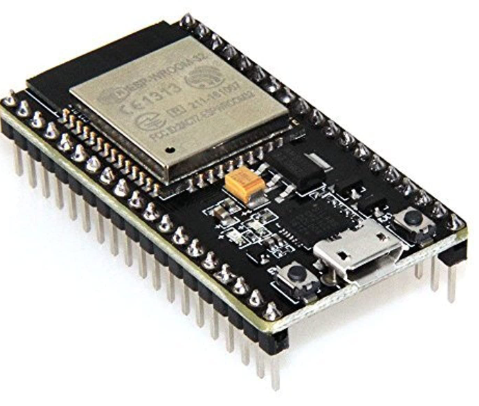
\includegraphics[scale=0.15]{images/Capitulo 4/3.1.1/S1/esp.png} & 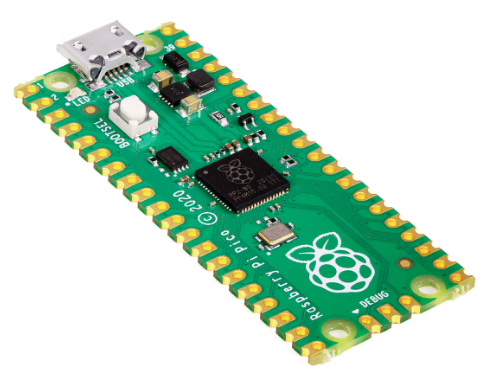
\includegraphics[scale=0.15]{images/Capitulo 4/3.1.1/S1/rasp.png} &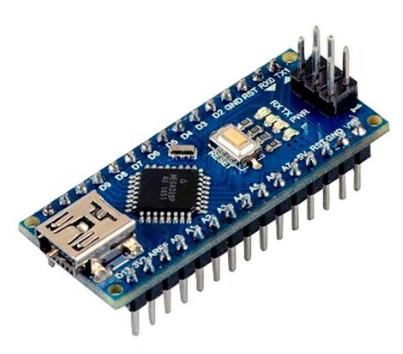
\includegraphics[scale=0.15]{images/Capitulo 4/3.1.1/S1/nano.png} & 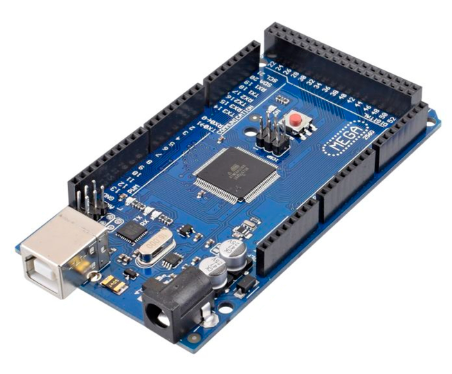
\includegraphics[scale=0.15]{images/Capitulo 4/3.1.1/S1/mega.png} \\ \hline
                Microcontrolador & Tensilica Xtensa 32-bit LX6 & RP2040 & ATMEGA328P & ATmega2560 \\
                Alimentación & 3.3 V & 3.3 V & 5 V & 5 V \\
                Corriente de operación & 20 a 240 mA & 1.3 a 93.5 mA & 20 a 40 mA & 20 a 50 mA \\
                Pines de comunicación & GPIO 24 & GPIO 26 & 14 Digitales 8 Analógicas & 54 Digitales y 16 Analógicas \\
                Dimensiones & 51 x 23 mm & 51 x 21 mm & 18 x 45 mm & 101.52 x 53.3 mm \\
                WIFI & Si & No & No & No \\
                Bluetooth & Si & No & No & No \\
                Frecuancia de trabajo & 240 Mhz & 133 MHz & 16 MHz & 16 MHz \\
                Precio & \$ 138.00 & \$ 114.00 & \$ 118.00 & \$ 272.00 \\
             \hline
        \end{tabular}
        }
    \label{tab:Tar_Des}%
\end{table}

Para la matriz de decisión, se tomaron en cuenta los siguientes requisitos:

\begin{itemize}
    \item Precio
    \item Accesibilidad
    \item Numero de pines
    \item Dimensiones
    \item Wifi
    \item Frecuencia de trabajo
\end{itemize}

La ponderación se realizo utilizando los siguientes valores para la evaluación de las diferentes opciones se encuentran en la tabla \ref{tab: Val des ap4}. Esta tiene fija un valor numérico que permite realizar un análisis cuantitativo para tomar alguna decisión de manera mas consciente

\begin{table}
    \centering
\caption{Ponderaciones para la matriz de decisión}
\label{tab: Val des ap4}
    \begin{tabular}{|c |c |} \hline 
         \multicolumn{2}{|c|}{Valores de ponderación}\\ \hline
         Excelente& 5\\ \hline
         Bueno& 4\\ \hline
         Regular& 3\\ \hline
 Malo&2\\ \hline
    \end{tabular}  
\end{table}

Se realizo la tabla de decisión para analizar las opciones mostradas en la tabla \ref{tab:Tar_Des} entonces se obtuvieron los valores que se muestran en la tabla\ref{tab:toma des tar des}


\begin{table}
    \centering
\caption{Ejemplo de toma de decisión de la tarjeta de desarrollo}
\label{tab:toma des tar des}
\resizebox{!}{17 cm}{
\begin{turn}{90}
    \begin{tabular}{|c|c|c|c|c|c|l|l|} \hline  
         Tarjeta de desarrollo&  \multicolumn{7}{|c|}{Caracteristica}\\ \hline  
         &  Precio&  Accesibilidad&  Numero de pines&  Dimensiones& Wifi & Frecuencia de trabajo&Total\\ \hline  
         \rowcolor[rgb]{ 1,  1,  0} 
 ESP32&  4&  5&  5&  4&  5& 5&28\\ \hline  
         Raspberry Pi Pico&  5&  3&  5&  4&  2& 4&23\\ \hline  
         Arduino Nano&  5&  5&  3&  5&  2& 2&22\\ \hline  
 Arduino Mega& 3& 5& 5& 3& 2& 2&20\\ \hline 
    \end{tabular}
    
    \end{turn}
    }
\end{table}

Con este proceso de toma de decisiones, se llego a la conclusión de que la tarjeta ESP32 es la que mejor se adapta a las necesidades del proyecto, es la opción que esta resaltada de la tabla \ref{tab:toma des tar des}

%\section{Ejemplo de cálculo de calor para un cilindro}\label{Ap:Temp_cilindro}

Si T1 > T2 el flujo de calor radial se da desde el interior hasta el exterior del contenedor.
\begin{center}
    
    $Q = -AK\frac{\Delta T}{\Delta \varepsilon} $
\end{center}

Se tienen dos áreas de las paredes de un cilindro hueco:
\begin{center}
    
$A_{\text{int}} = 2\pi r_1 L$ 
\end{center}
\begin{center}
    
$A_{\text{ext}} = 2\pi r_2 L$
\end{center}
Se toma un radio de referencia r que varía desde r1 hasta r2 

Sustituyendo el área de la pared de un cilindro, tomando en cuenta el radio de referencia r.


\[
Q = -(2\pi rL) \frac{dT}{dr}
\]

\[
\frac{-Q}{2\pi L} \int_{r_1}^{r_2} \frac{dr}{r} = k \int_{T_1}^{T_2} dT
\]

\[
\frac{-Q}{2\pi L} (\ln r_2 - \ln r_1) = k(T_2 - T_1)
\]

\[
Q = \frac{k2\pi L(T_1 - T_2)}{\ln(r_2/r_1)}
\]

Para las tapas del cilindro:

\[
Q = \frac{k2\pi r^2 (T_2 - T_1)}{\varepsilon}
\]
%\section{Ejemplo cálculo de temperatura final}\label{Ap:temp_final}

Partiendo de la ley de Newton para la transferencia de calor, se tiene:\cite{LeyNewtonCalor}

\[Q = h \cdot A \cdot \Delta T\]

Siendo:

\begin{itemize}
  \item Q es la tasa de transferencia de calor
  \item h es el coeficiente de transferencia de calor por convección
  \item A es el área de contacto
  \item $\delta$T es la diferencia de temperatura entre el objeto y el fluido
\end{itemize}
Se retoman los cálculos obtenidos para un cilindro de acuerdo con la ley de Fourier y la ley de Newton para la transferencia de calor.
\[Q_{\text{conducción}} = Q_{\text{convección}}\]

\[\frac{{2\pi L K (T_i - T_f)}}{{\ln\left(\frac{{r_0}}{{r_1}}\right)}} = h A (T_f - T_{\text{aire}})
\]
Se despeja Tf para conocer la temperatura que tendrá el compostador en la cara externa.
\[T_f \left(hA+\frac{2\pi LK}{\ln\left(\frac{r_0}{r_1}\right)}\right) = \frac{2\pi LKT_i}{\ln\left(\frac{r_0}{r_1}\right)} + hAT_{\text{aire}}
\]
Finalmente se obtiene:
\[T_f = \frac{\left(\frac{2\pi LKT_i}{\ln\left(\frac{r_0}{r_1}\right)} + hAT_{\text{aire}}\right)}{\left(hA+\frac{2\pi LK}{\ln\left(\frac{r_0}{r_1}\right)}\right)}
\]
Se ha propuesto, usar tres grados Celsius como temperatura del aire. Es importante señalar que la constante de convección del aire puede variar dependiendo de diversos factores, como la velocidad del flujo de aire, la temperatura y la presión por lo que su valor se encuentra en un rango de cinco a veinticinco W/(m²·K), por lo que se propondrá utilizar un valor de veinticuatro W/(m²·K). Proponiendo que al interior del contenedor exista una temperatura (Ti) de cincuenta grados Celsius.

Se presentan los valores a sustituir:

\begin{itemize}
  \item L=0.73 m
  \item r0=0.228 m
  \item A es el área de contacto
  \item r1=0.227 m
  \item K=51.9 W/mK
  \item h=24 W/(m²·K)
  \item Ti=50°C = 323K
  \item Taire=3°C=276K
\end{itemize}
Sustituyendo los valores en la temperatura final calculada (Tf), se tiene:

\[\frac{\left(\frac{{2\pi \cdot 0.73 \, \text{m} \cdot 51.9 \, \text{W/mK}}}{{\ln\left(\frac{{0.228 \, \text{m}}}{{0.227 \, \text{m}}}\right)}}\right) \cdot (323 \, \text{K})
+ (24 \, \text{W/(m}^2 \, \text{K}) \cdot 276 \, \text{K} \cdot \left((2\pi \cdot 0.228 \, \text{m} \cdot 0.73 \, \text{m}) + (2\pi \cdot 0.228 \, \text{m}^2)\right))
}{\left(24 \, \text{W/(m}^2 \, \text{K})\right) \cdot \left(\left(2\pi \cdot 0.227 \, \text{m} \cdot 0.73 \, \text{m}\right) + \left(2\pi \cdot 0.227 \, \text{m}^2\right)\right) + \left(\frac{{2\pi \cdot 0.73 \, \text{m} \cdot 51.9 \, \text{W/mK}}}{{\ln\left(\frac{{0.228 \, \text{m}}}{{0.227 \, \text{m}}}\right)}}\right)
}
\]
Se obtiene la potencia sustituyendo Tf en alguno de los lados de la igualdad, obteniendo:

\[Q = \left(24 \, \text{W/(m}^2 \, \text{K}\right) \cdot \left(\left(2\pi \cdot 0.228 \, \text{m} \cdot 0.73 \, \text{m}\right) + \left(2\pi \cdot 0.228 \, \text{m}^2\right)\right) \cdot (323 \, \text{K} - 322.97 \, \text{K})
\]
\[Q = 1.547 \, \text{kW}
\]
%\section{Estudios Térmicos}
\label{Ap:Estudio_termico}


\begin{figure}[h!]
            \centering
            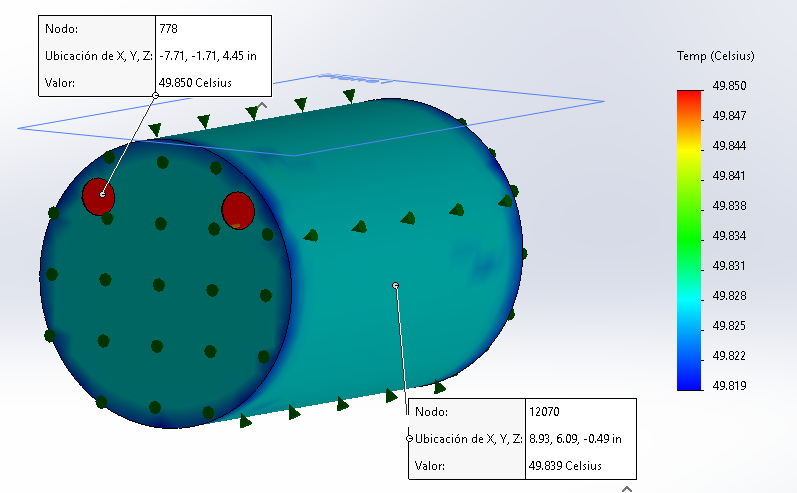
\includegraphics[scale=0.4]{images/Capitulo 4/s5/Contenedor/Est_Termicos/termicosf_3.png}
            \caption{Estudio térmico del contenedor}
            \label{fg:Estermico}
     \end{figure}

Lo que se puede observar aquí es que el calor pasa casi en su totalidad a la cara externa ya que se encuentra a .011 grados de la temperatura interna, lo que generará grandes pérdidas de calor. En un proceso de análisis el equipo se percató que este comportamiento podría representar un riesgo para quien manipule el dispositivo, puesto que si el usuario llega a tocar la parte externa, podría quemarse.

        \begin{figure}[h!]
            \centering
            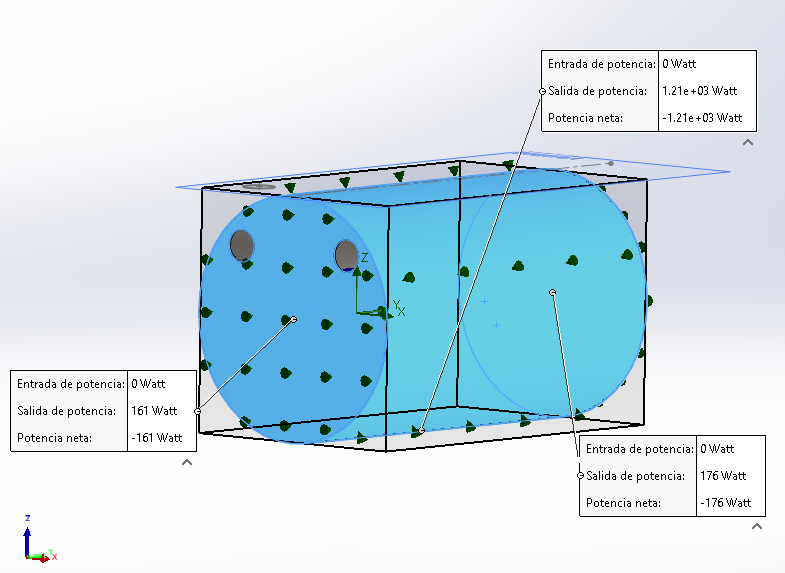
\includegraphics[scale=0.4]{images/Capitulo 4/s5/Contenedor/Est_Termicos/Potenciamod_3.png}
            \caption{Salida de potencia del modelo}
            \label{fg:Psf}
        \end{figure} \newpage

          \begin{figure}[h!]
            \centering
            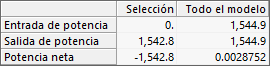
\includegraphics[scale=0.8]{images/Capitulo 4/s5/Contenedor/Potencia_total_modelo.png}
            \caption{Salida de Potencia total del modelo}
            \label{fg:Ptm}
        \end{figure}
        
Como se mencionó previamente, al pasar casi todo el calor a la cara externa del contenedor presentándose una potencia de salida de 1.544k W (Figura \ref{fg:Ptm}), lo que representa una gran pérdida de calor.

Tratando de contrarrestar este comportamiento que no es deseable para el funcionamiento del compostador se propone cubrir el contenedor un material aislante, en este caso se plantea utilizar fibra de vidrio, realizando la simulación recubriendo las paredes externas con este nuevo material (Figura \ref{fg:ETFV}).

    \begin{figure}[h!]
            \centering
            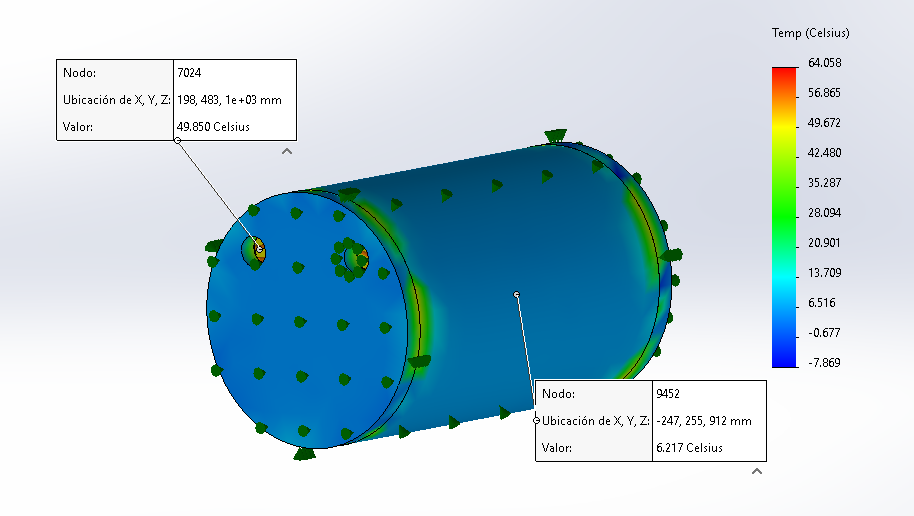
\includegraphics[scale=0.4]{images/Capitulo 4/s5/Contenedor/Est_Termicos/termico3_fibra.png}
            \caption{Estudio térmico con fibra de vidrio}
            \label{fg:ETFV}
        \end{figure}
Como se puede observar, los resultados mejoraron considerablemente, puesto que las caras externas se encuentras 3.217 grados por encima de la temperatura ambiental propuesta (3°C). Lo que permite mantener el calor al interior del contenedor, y en caso de que el usuario llegue a tocarlo, no se queme.

Estos resultados son coherentes ya que la conductividad térmica del acero corresponde a 51.9 W/mK y la conductividad de la fibra es de tan solo 0.04 W/mK, 1297.5 veces más pequeña que la conductividad del acero.

Y esto se puede observar en la potencia de salida, presentando los siguientes resultados (Figura \ref{fg:PmFV}).

  \begin{figure}[h]
            \centering
            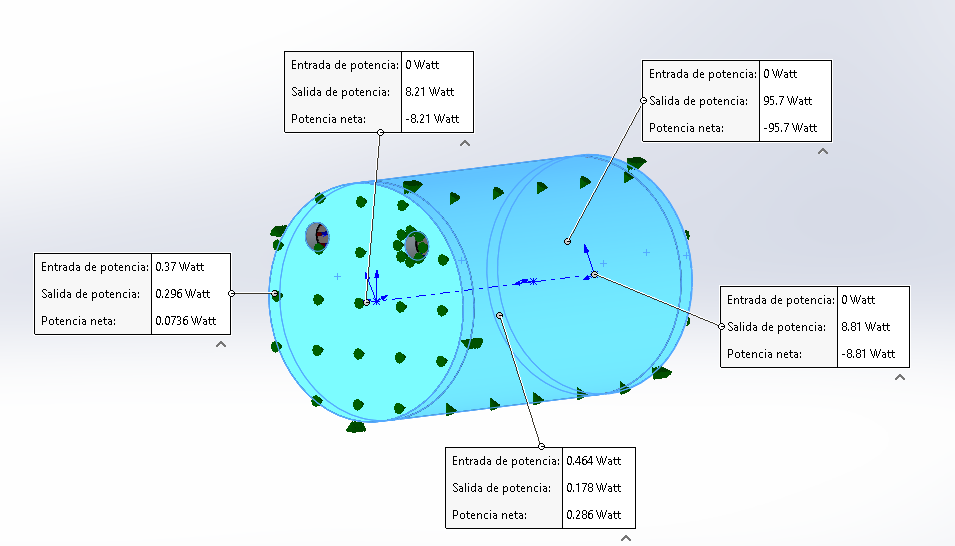
\includegraphics[scale=0.4]{images/Capitulo 4/s5/Contenedor/Est_Termicos/Potenciamod_3_fibra.png}
            \caption{Salida de Potencia con fibra de vidrio}
            \label{fg:PmFV}
    \end{figure}\newpage
        
        \begin{figure}[h]
            \centering
            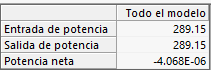
\includegraphics[scale=0.9]{images/Capitulo 4/s5/Contenedor/Est_Termicos/Potencia_fibra3.png}
            \caption{Salida de potencia total con fibra de vidrio}
            \label{fg:PTFV}
        \end{figure}
        
Como se puede apreciar en los resultados obtenidos con la potencia de salida total del modelo con fibra de vidrio (Figura \ref{fg:PTFV}) , es cinco veces menor en comparación a la salida de potencia total del modelo sin aislante térmico, lo que permite observar una reducción significativa del calor transmitido.

    Como se puede observar, los resultados obtenidos son bastante cercanos a los presentados teóricamente por otro lado, considerar la fibra de vidrio, puede beneficiar en gran manera el funcionamiento del circuito, ya que como se observó reduce la pérdida de calor, lo que en consecuencia evitaría el estar encendiendo continuamente las resistencias que calentarán el interior del contenedor, alargando así su vida útil y reduciendo de igual manera la energía consumida durante su funcionamiento.

Por otro lado, es bien sabido que la temperatura en la Ciudad de México cambia constantemente a lo largo del año, por lo que se propuso efectuar las simulaciones considerando una temperatura promedio de 16°C de acuerdo con datos del INEGI \cite{TempINEGI} y otra de 31.6°C siendo la temperatura más alta del año 2022 registrada en la ciudad de México de acuerdo a datos de la Secretaría de  Gestión Integral de Riesgos y Protección Civil (SGIRPC) \cite{Temp31}. Cabe señalar que la temperatura de 3°C se propuso debido a que se tiene pensado que la gran mayoría de pruebas se realizarán en épocas de días fríos del siguiente semestre, por lo que resultaba de interés observar el comportamiento del contenedor en un escenario similar. \newpage

Para 16°C sin aislante térmico, se obtuvieron los siguientes resultados:

\begin{figure}[h!]
            \centering
            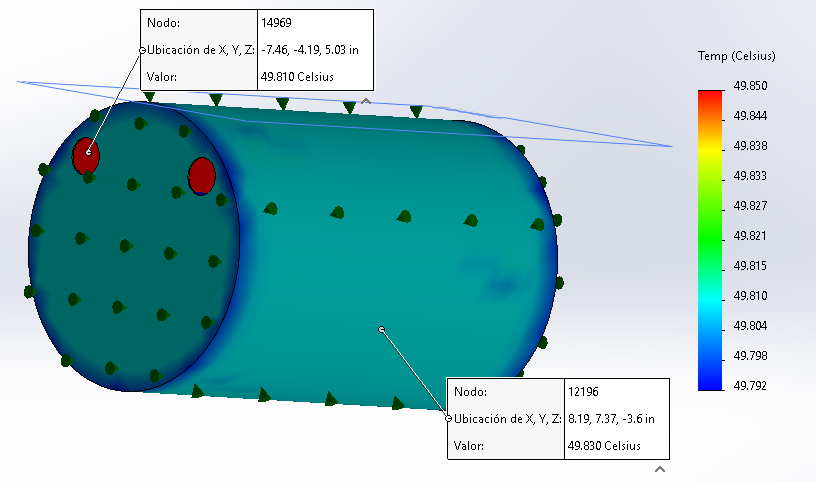
\includegraphics[scale=0.5]{images/Capitulo 4/s5/Contenedor/Est_Termicos/termicosf_16.png}
            \caption{Estudio térmico para una temperatura de 16°C}
            \label{fg:termico16}
        \end{figure}

        \begin{figure}[h!]
            \centering
            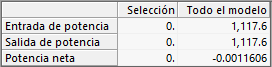
\includegraphics[scale=0.9]{images/Capitulo 4/s5/Contenedor/Est_Termicos/Potenciasf_16.png}
            \caption{Salida de potencia temperatura de 16°C}
            \label{fg:Potencia16}
        \end{figure}

Para 16°C con aislante térmico (fibra de vidrio), se obtuvieron los siguientes resultados:

\begin{figure}[h!]
            \centering
            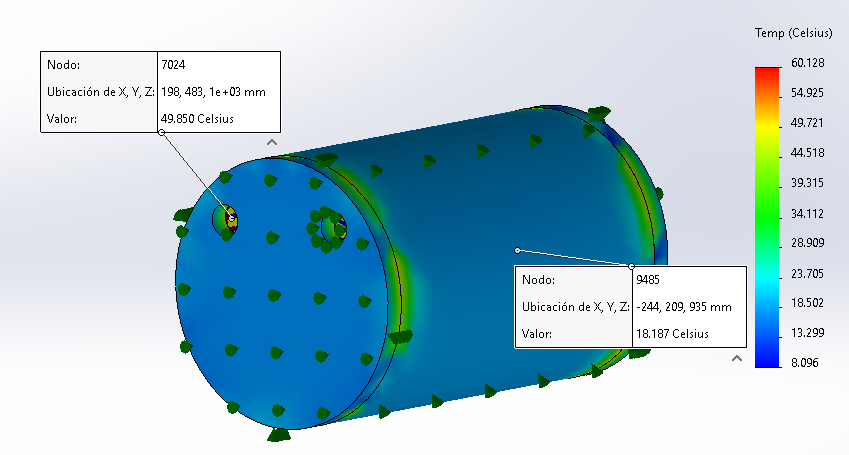
\includegraphics[scale=0.5]{images/Capitulo 4/s5/Contenedor/Est_Termicos/termico16_fibra.png}
            \caption{Estudio térmico para una temperatura de 16°C}
            \label{fg:termico16_fibra}
        \end{figure}

        \begin{figure}[h!]
            \centering
            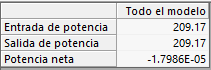
\includegraphics[scale=0.9]{images/Capitulo 4/s5/Contenedor/Est_Termicos/Potencia_fibra16.png}
            \caption{Salida de potencia temperatura de 16°C}
            \label{fg:Potencia16_fibra}
        \end{figure}

Para 31.6°C sin aislante térmico, se obtuvieron los siguientes resultados:

\begin{figure}[h!]
            \centering
            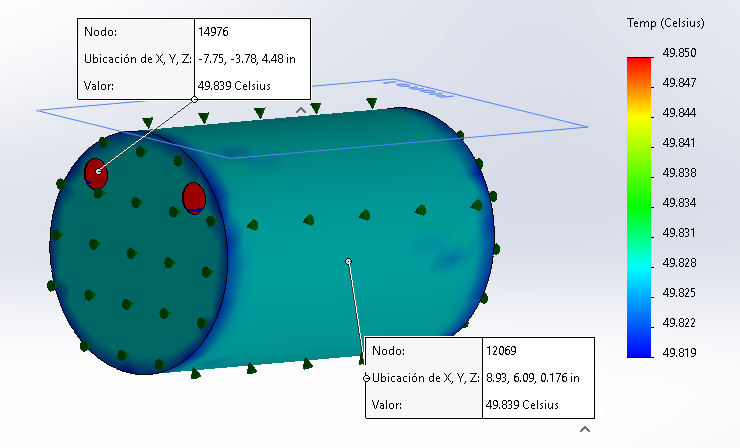
\includegraphics[scale=0.5]{images/Capitulo 4/s5/Contenedor/Est_Termicos/termicosf_31.6.png}
            \caption{Estudio térmico para una temperatura de 31.6°C}
            \label{fg:termico31}
        \end{figure}

        \begin{figure}[h!]
            \centering
            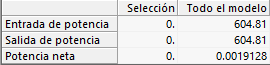
\includegraphics[scale=0.9]{images/Capitulo 4/s5/Contenedor/Est_Termicos/Ptenciasf_31.6.png}
            \caption{Salida de potencia temperatura de 31.6°C}
            \label{fg:Potencia31}
        \end{figure}

Para 31.6°C con aislante térmico (fibra de vidrio), se obtuvieron los siguientes resultados:

\begin{figure}[h!]
            \centering
            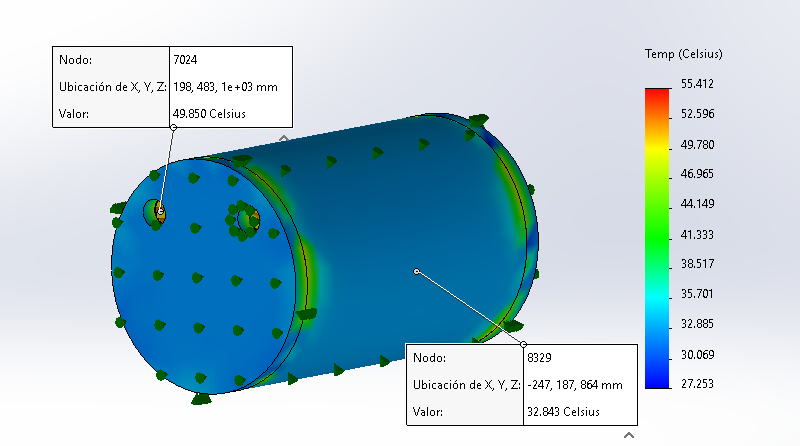
\includegraphics[scale=0.5]{images/Capitulo 4/s5/Contenedor/Est_Termicos/termico31_fibra.png}
            \caption{Estudio térmico para una temperatura de 31.6°C con aislante térmico}
            \label{fg:termico31_fibra}
        \end{figure}

        \begin{figure}[h!]
            \centering
            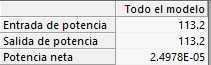
\includegraphics[scale=0.9]{images/Capitulo 4/s5/Contenedor/Est_Termicos/Potencia_fibra31.png}
            \caption{Salida de potencia temperatura de 31.6°C con aislante térmico}
            \label{fg:Potencia31_fibra}
        \end{figure}
%\section{Cálculos de la estructura}
\label{Ap:Estructura}

\begin{center}
    $\tau=FdSin\theta$
\end{center}

Si el ángulo $\theta$ se considera máximo, al aplicar la carga con un ángulo de $90 ^oC$ se tiene.

Donde: \\
$F$ es el peso de la materia orgánica en $[N]$\\
$d$ es la distancia del eje de rotación al extremo de la pala en $[m]$\\
$\theta$ es el ángulo de aplicación de la fuerza en $[^oC]$

\section{Potencia Consumida}\label{Ap:Eje}

\begin{center}
  $\omega = \frac{\theta}{t} $  
\end{center}
Selección
Donde: \\
$\theta$ son las vueltas en radianes \\
$t$ es el tiempo en segundos


\begin{center}
 $P_{cons}=M_t * \omega$   
\end{center}

Donde: \\

$M_t$ es el Momento de torsión $\tau$ \\
$\omega$ es la velocidad angular previamente calculada
\newpage

\section{Diseño de la transmisión por bandas}\label{Ap:Eje }

\begin{figure}[h]
    \centering
        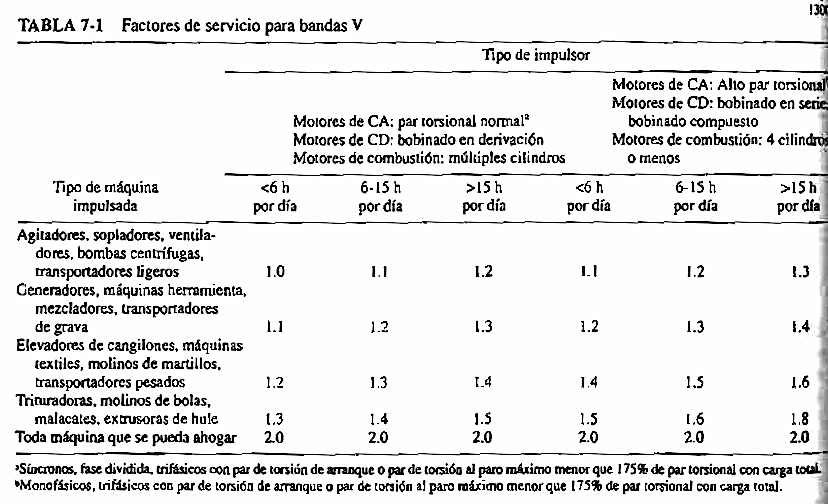
\includegraphics[scale=0.8]{images/Capitulo 4/s5/Factores de servicio.png}
        \caption{Factores de Servicio para bandas V}\cite{Mott}
    \label{fg:Factores}
\end{figure}

\begin{figure}[h]
    \centering
        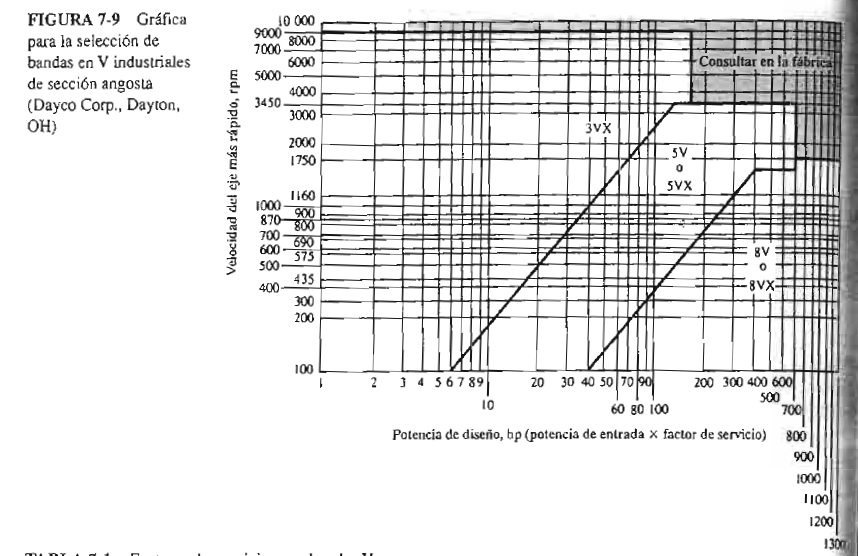
\includegraphics[scale=0.7]{images/Capitulo 4/s5/Grafica para la seleccion de bandas.png}
        \caption{Gráfica para la selección de bandas}\cite{Mott}
    \label{fg:Bandas}
\end{figure}

\begin{figure}[h]
    \centering
        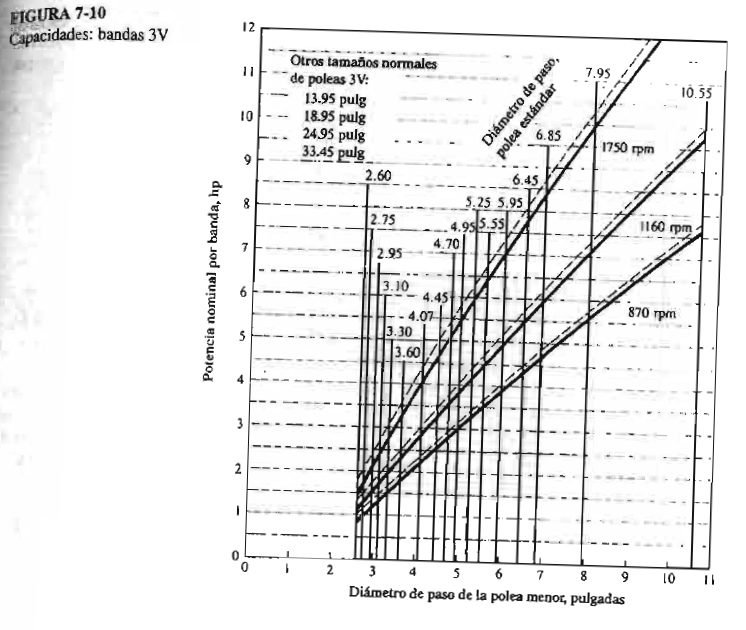
\includegraphics[scale=1]{images/Capitulo 4/s5/Capacidad 3V.png}
        \caption{Capacidad Banda 3V}\cite{Mott}
    \label{fg:Banda3V}
\end{figure}

\begin{figure}[h!]
    \centering
        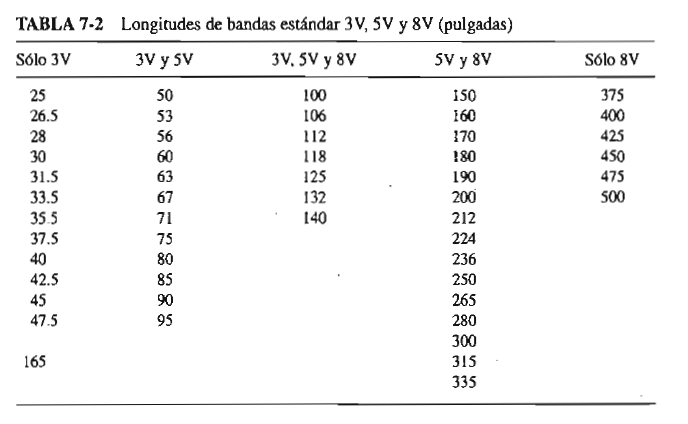
\includegraphics[scale=1.1]{images/Capitulo 4/s5/Longitudes bandas.png}
        \caption{Longitudes de Bandas estándar}\cite{Mott}
    \label{fg:Longitud}
\end{figure}
\newpage

\begin{figure}[h!]
    \centering
        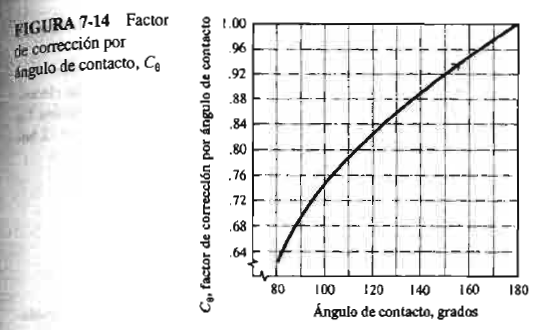
\includegraphics[scale=1]{images/Capitulo 4/s5/Factor theta.png}
        \caption{Factor theta}\cite{Mott}
    \label{fg:theta}
\end{figure}
\begin{figure}[h!]
    \centering
        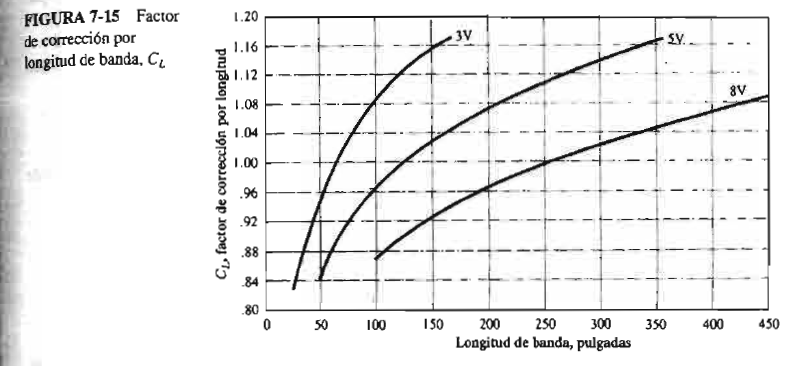
\includegraphics[scale=0.9]{images/Capitulo 4/s5/Factor L.png}
        \caption{Factor Longitud}\cite{Mott}
    \label{fg:L}
\end{figure}
\newpage


\section{Diseño de la cuña}
\label{Ap:Eje Seleccion}
\begin{figure}[h!]
    \centering
        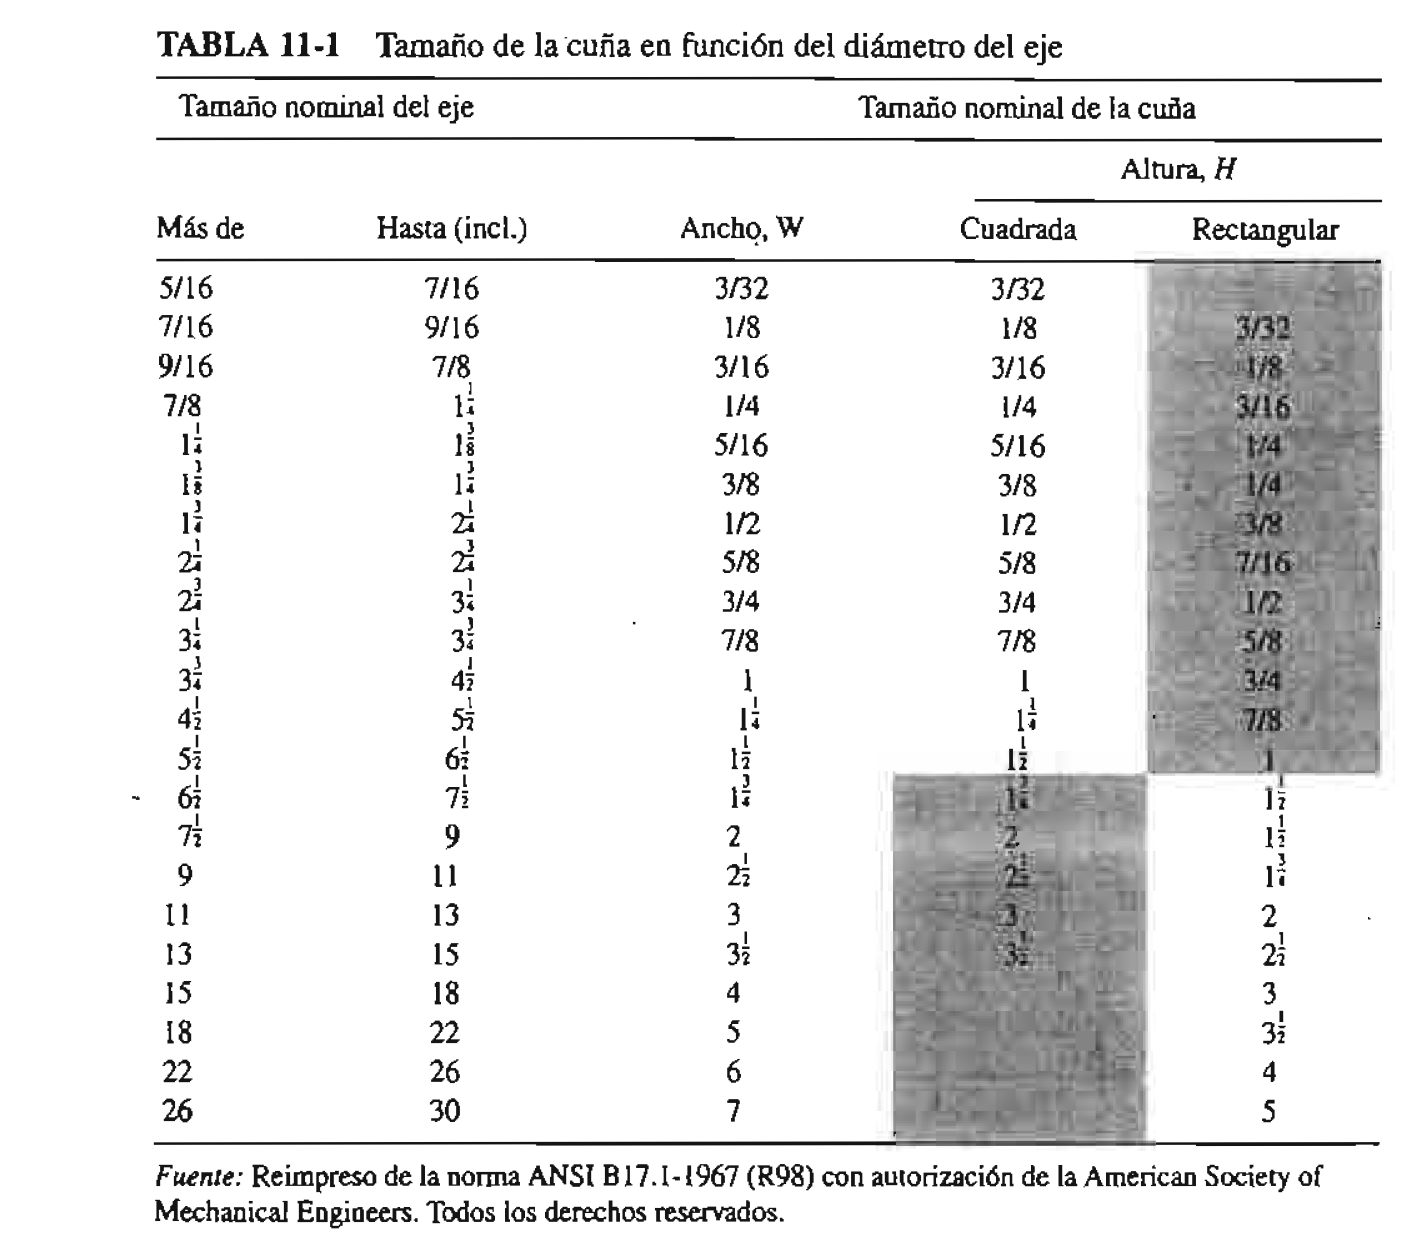
\includegraphics[scale=0.5]{images/Capitulo 4/s5/Tamanos Cuna.png}
        \caption{Tamaño de cuña en función del diámetro del eje }\cite{Mott}
    \label{fg:Tamaños Cuña}
\end{figure}
\newpage

\section{Diseño del eje de Aireación}\label{Ap:Eje Seleccion}
\begin{center}
    $D=\sqrt[3]{\frac{32*N}{\pi}*\sqrt{(K_t*\frac{M}{s'n})^2+ \frac{3}{4}*(\frac{T}{S_y})^2}}$
\end{center}

Donde: \\
$K_t$ es la concentración de esfuerzos que se producen por variaciones geométricas. \\
$N$ Factor de diseño.\\
$s'n$ es el valor de la resistencia a la fatiga según el material seleccionado.\\
$M$ momentos flexionantes. \\
$T$ es el torque al que se ve sometido el eje. \\
$S_y$ esfuerzo de fluencia.

\begin{center}
    $s'n =  sn*C_m*C_{st}*C_r*C_s$
\end{center}

Donde: \\
s’n: valor de la resistencia real a la fatiga. \\
sn: es el valor de resistencia a la fatiga teórico. \\
$C_m$: factor de material. \\
$C_{st}$: factor de tipo de esfuerzo. \\
$C_r$: factor de confiabilidad \\
$C_s$: factor de tamaño \\

\begin{figure}[h]
    \centering
        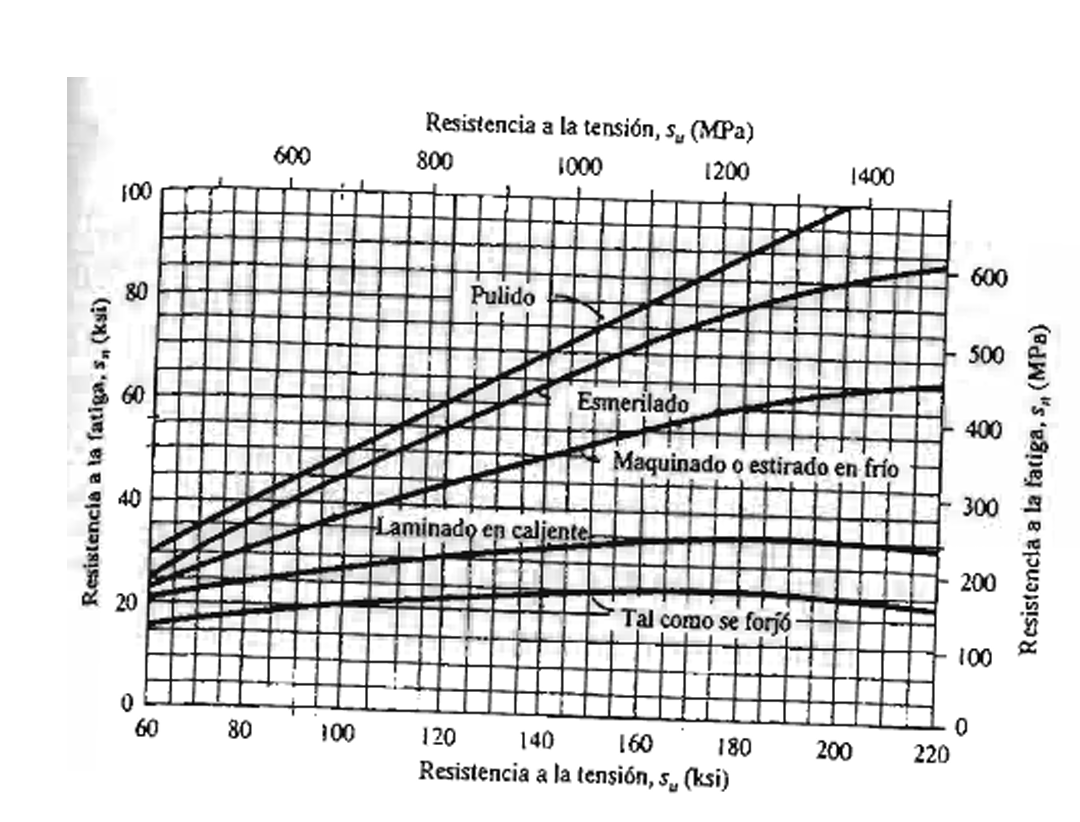
\includegraphics[scale=0.6]{images/Capitulo 4/s5/Resistencia a la fatiga.png}
        \caption{Resistencia a la fatiga}\cite{Mott}
    \label{fg:Res_fat}
\end{figure}
\begin{figure}[p]
    \centering
        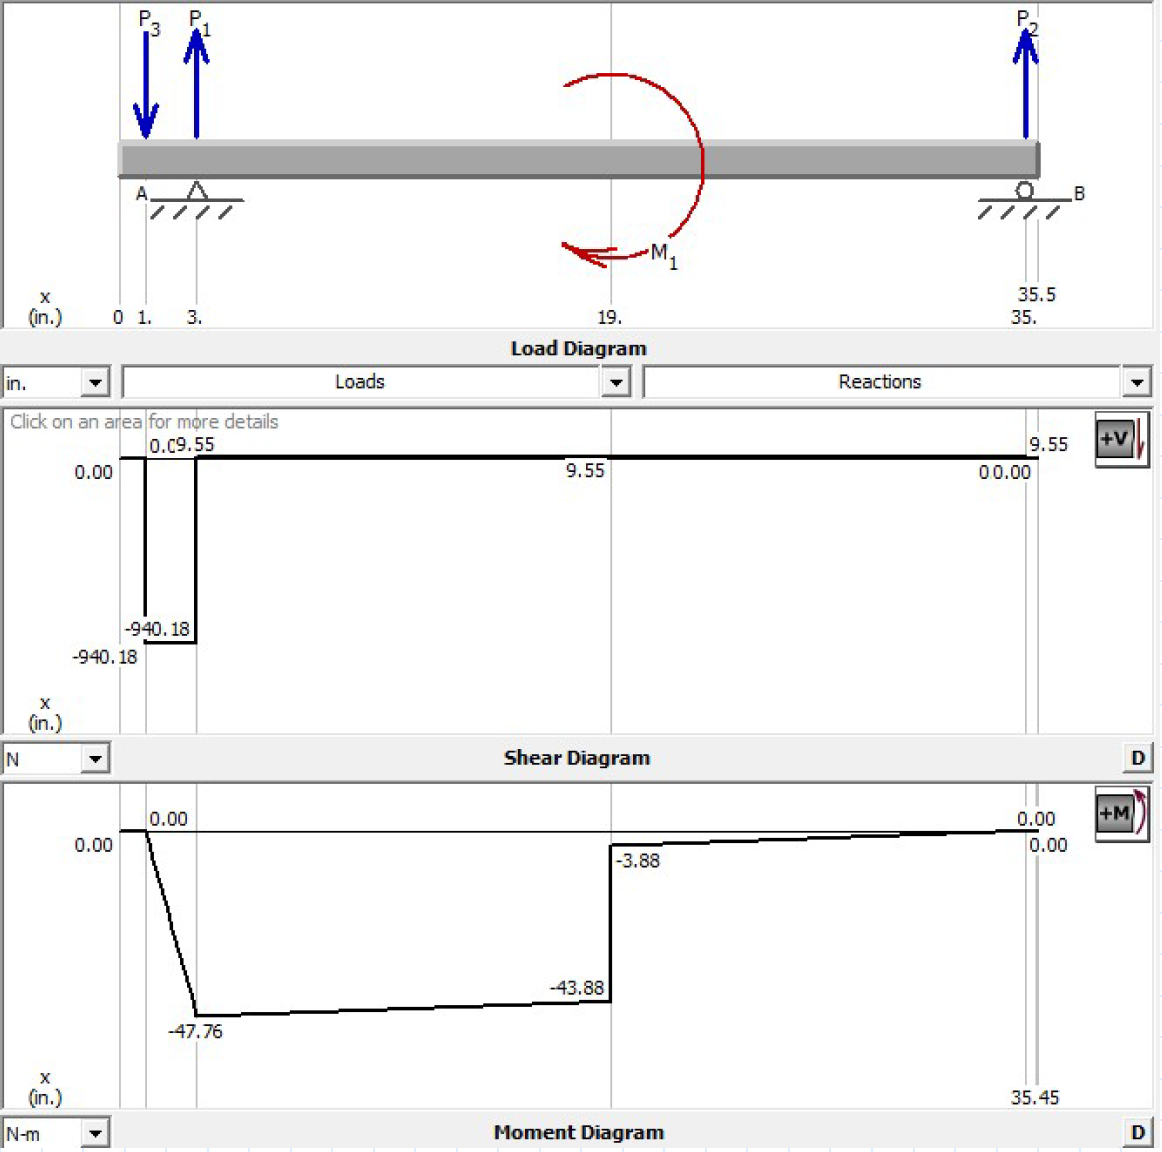
\includegraphics[scale=0.8]{images/Capitulo 4/s5/1 pala fuerzas.png}
        \caption{Fuerzas, Esfuerzos y Momentos del lado del eje con 1 pala}
    \label{fg:1palaF}
\end{figure}
\begin{figure}[p]
    \centering
        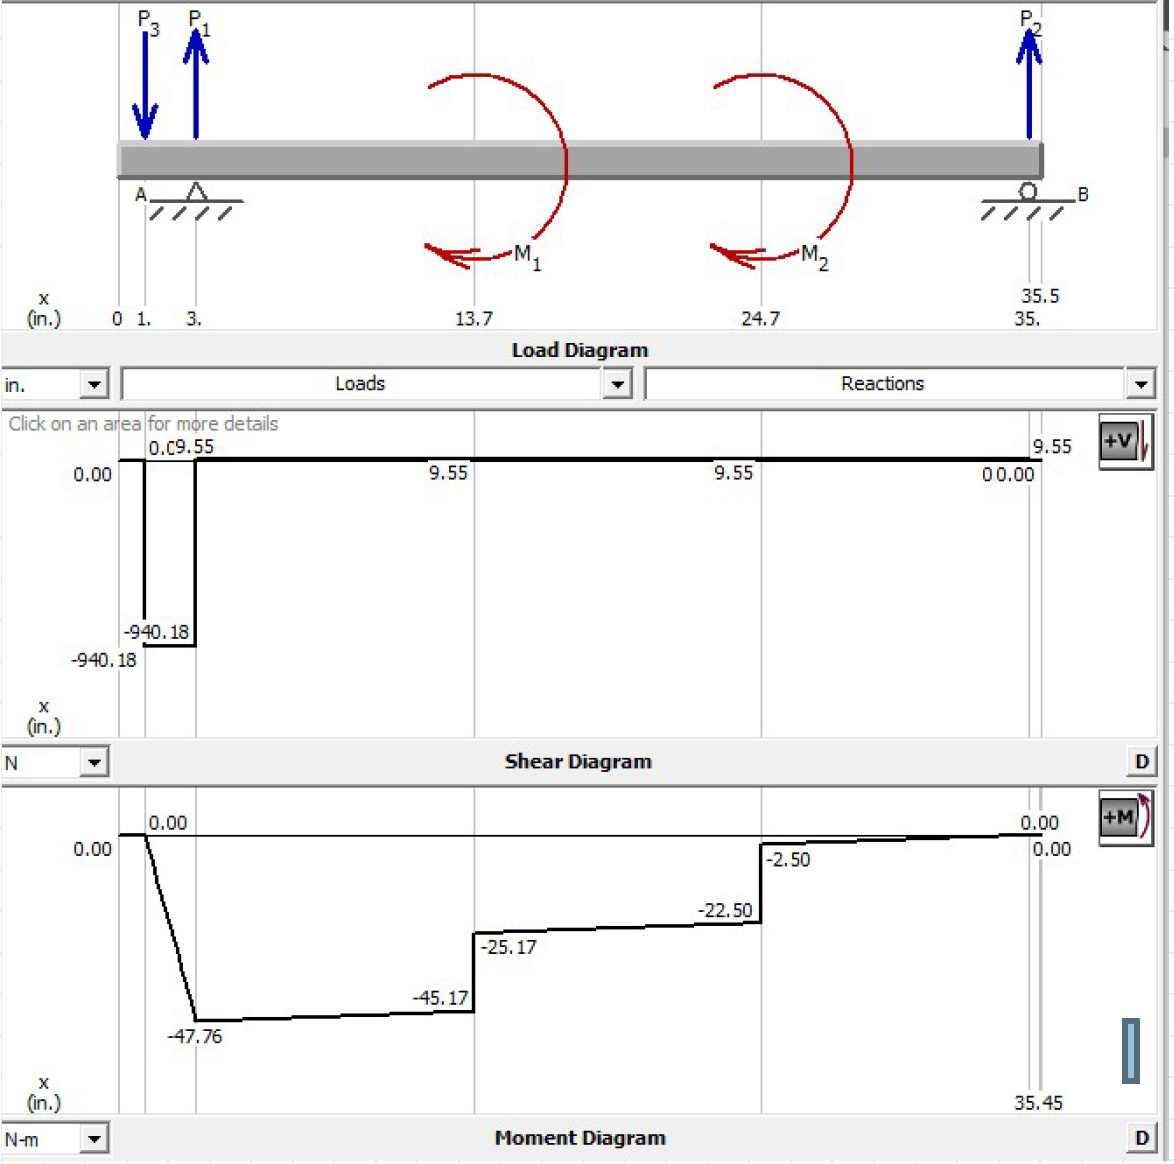
\includegraphics[scale=0.8]{images/Capitulo 4/s5/2 palas fuerzas.png}
        \caption{Fuerzas, Esfuerzos y Momentos del lado del eje con 2 palas}
    \label{fg:2palasF}
\end{figure}
%\section{Ejemplo de procedimiento PID}\label{Ap:control}

A continuación, se presentará el procedimiento para la realización del control PID que se llevará a cabo.  

En un primer momento, se realiza la comunicación entre Arduino y simulink (Figura \ref{fg:Comunicacion}) para obtener las mediciones del sensor, es importante señalar, que se toma en cuenta la pendiente de operación del sensor para poder procesar los datos en simulink.

\begin{figure}[h!]
            \centering
            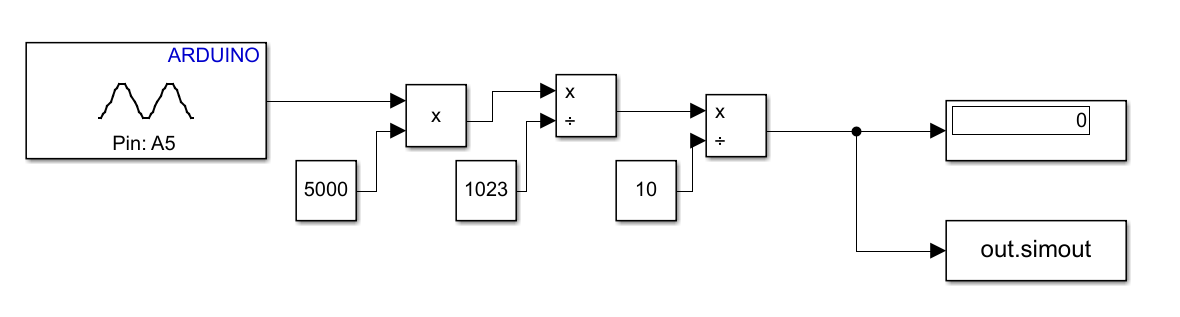
\includegraphics[scale=0.4]{images/Capitulo 3/3.1.2/comunicacion.png}
            \caption{Comunicación Simulink-Arduino}
            \label{fg:Comunicacion}
        \end{figure}
Una vez que la comunicación se realizó de manera correcta, se podrá ver en simulink la curva de calentamiento del sensor, es importante establecer un tiempo que sea los suficientemente largo para observar la estabilización del valor máximo que se alcanza.
En este caso se observa como parte de la temperatura ambiental y aumenta la temperatura, presentando un comportamiento logarítmico (Figura \ref{fg:Curva_calent}), este comportamiento corresponde a un sensor LM35 sin embargo, se espera un comportamiento similar en otros sensores como el DS18B20.

\begin{figure}[h!]
            \centering
            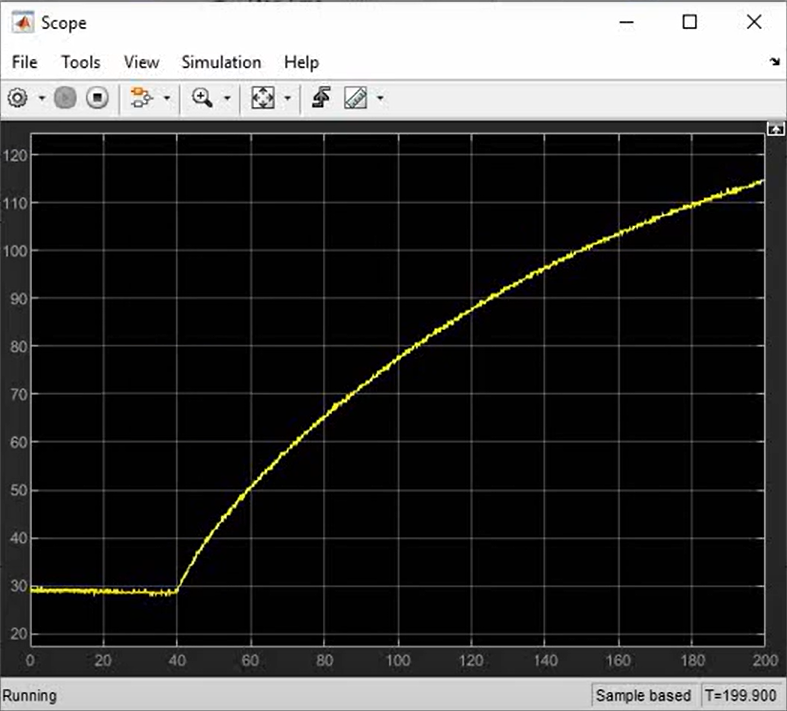
\includegraphics[scale=0.4]{images/Capitulo 3/3.1.2/curva_calentamiento.png}
            \caption{Curva de calentamiento LM35}
            \label{fg:Curva_calent}
        \end{figure}
Con las mediciones realizadas, se procede a obtener la función de transferencia del sistema (Figura \ref{fg:Func_transfer}).

\begin{figure}[h!]
            \centering
            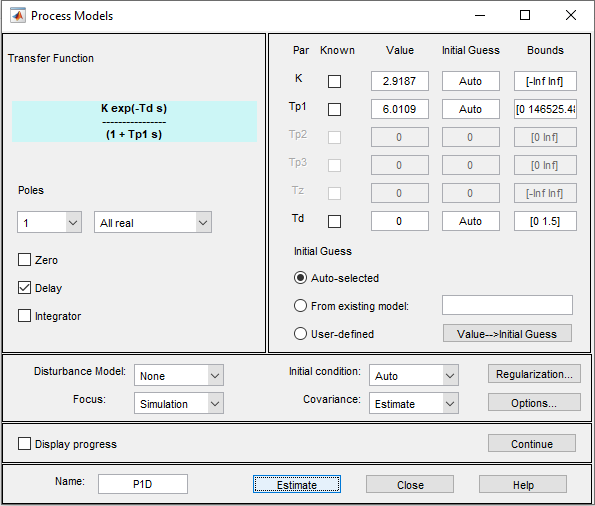
\includegraphics[scale=0.5]{images/Capitulo 3/3.1.2/Ftransferencia.png}
            \caption{Función de transferencia obtenida con Simulink}
            \label{fg:Func_transfer}
        \end{figure}
        
        
Se agrega el PID a la comunicación de Simulink y Arduino (Figura \ref{fg:PID+CSA}) y se ajusta la señal para que el control de comporte de la manera deseada, evitando un sobre impulso o que el sistema tarde demasiado en llegar al valor requerido (Figura \ref{fg:PIDTS}).

\begin{figure}[h!]
            \centering
            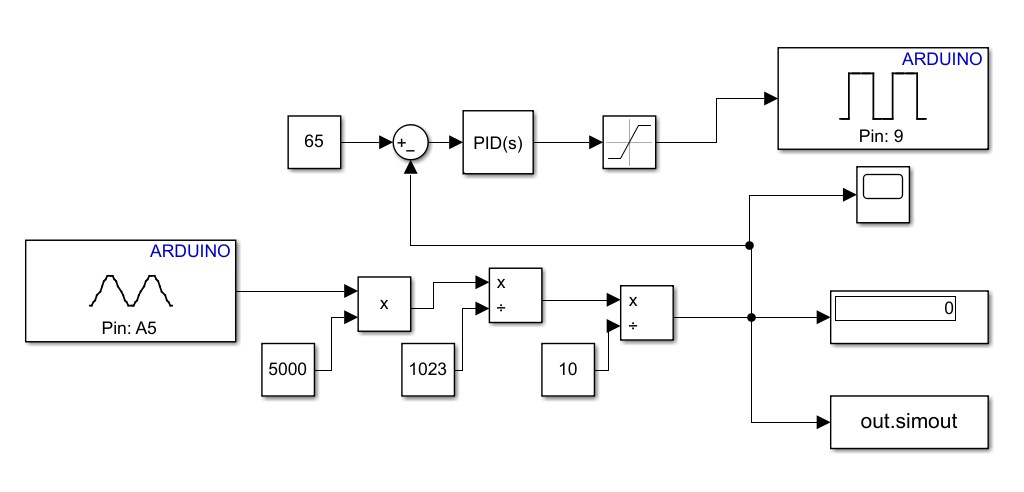
\includegraphics[scale=0.3]{images/Capitulo 3/3.1.2/ControlPID_comSimu.png}
            \caption{Control PID y comunicación Simulink-Arduino}
            \label{fg:PID+CSA}
        \end{figure}

\begin{figure}[h!]
            \centering
            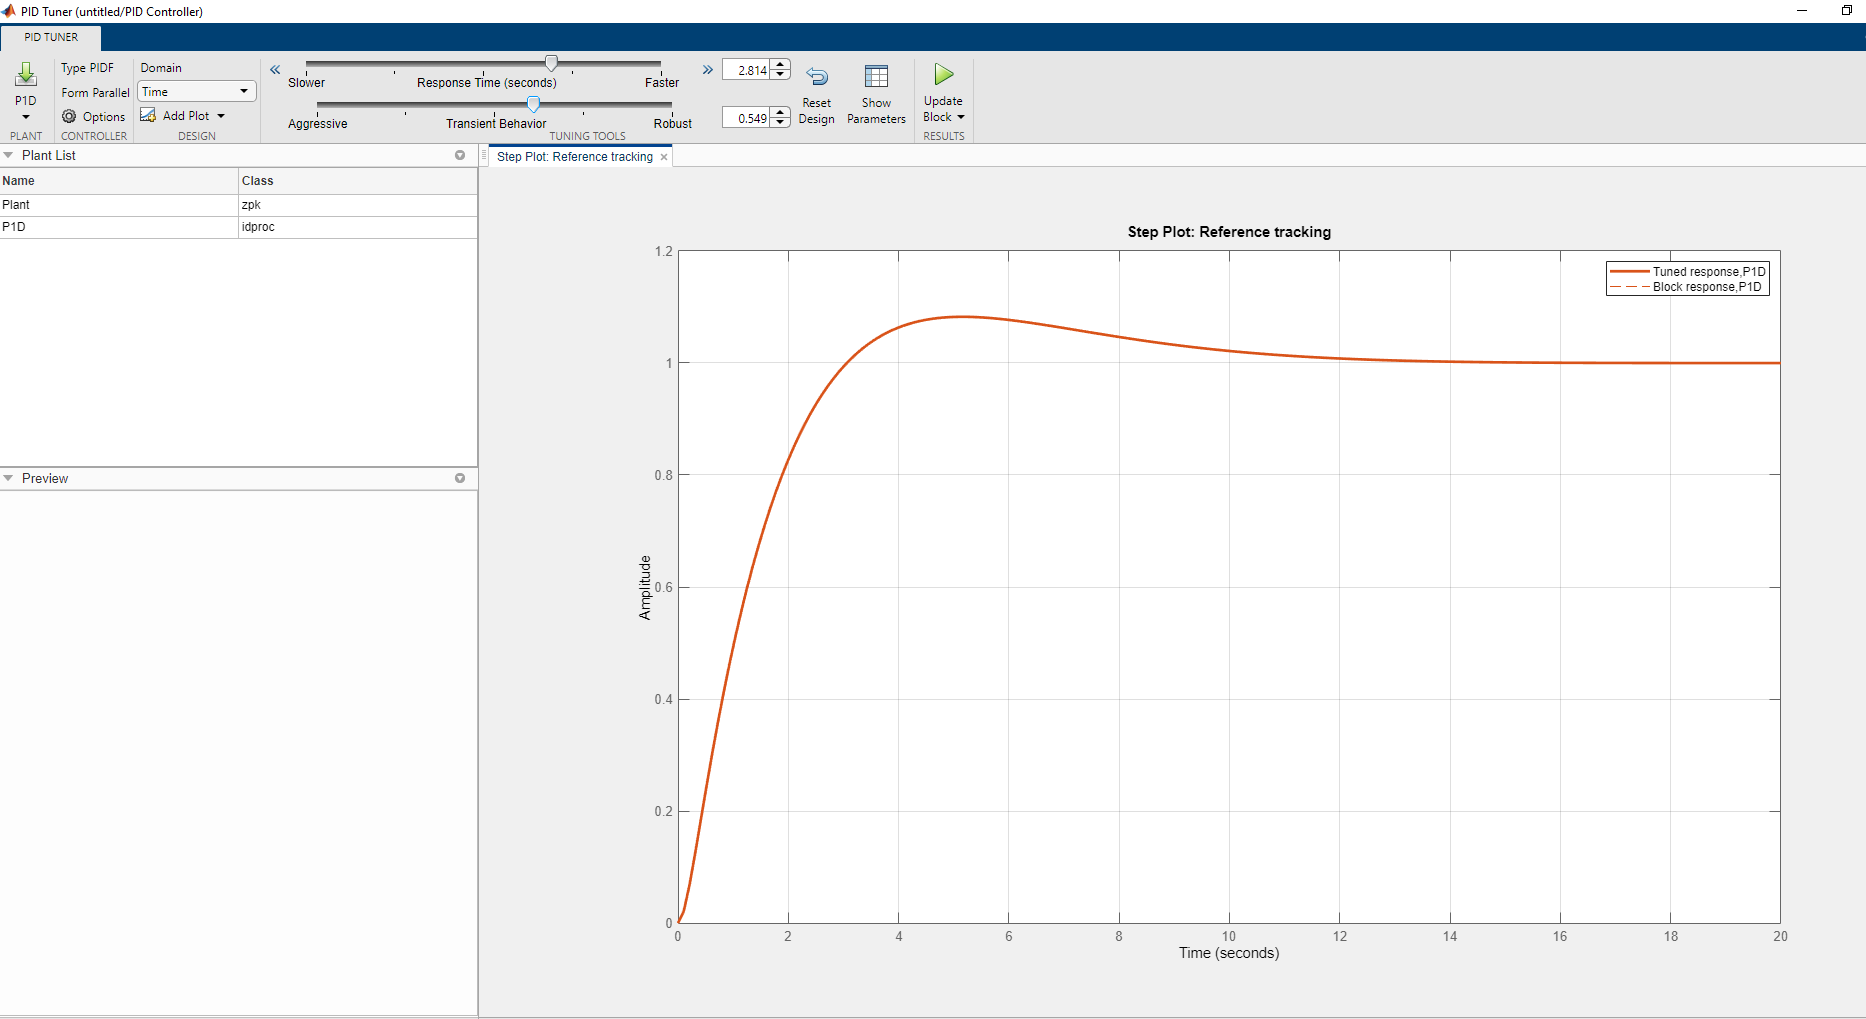
\includegraphics[scale=0.25]{images/Capitulo 3/3.1.2/PID_Tuner.png}
            \caption{PID Tuner Simulink}
            \label{fg:PIDTS}
        \end{figure}
        
%\section{Simulaciones sistema de ventilación}\label{Ap:Vetilacion}

     Se realizaron algunas simulaciones con distintas distribuciones de los ventiladores, con el propósito de observar su comportamiento y elegir la más adecuada a las necesidades del compostador, se obtuvieron los siguientes resultados:

     \begin{figure}[h!]
            \centering
            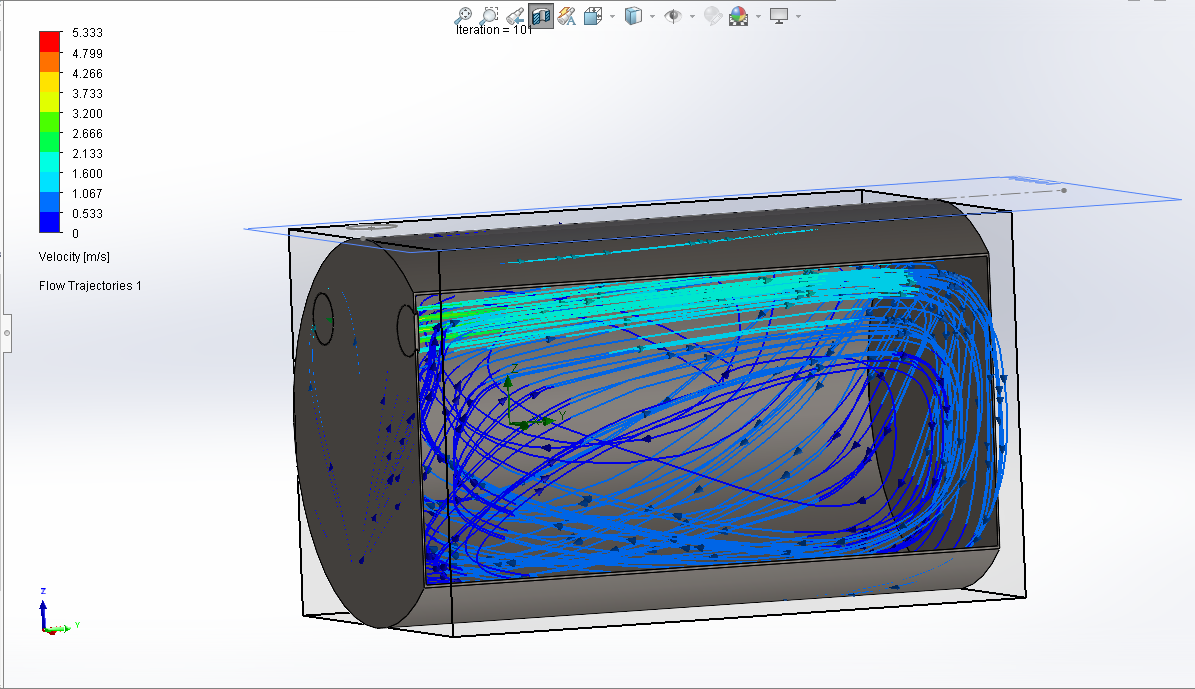
\includegraphics[scale=0.4]{images/Capitulo 4/s5/Contenedor/flow1.png}
            \caption{Configuración de ventiladores en la misma cara lateral}
            \label{fg:ventilador_mcara}
     \end{figure}
    Esta primera configuración \ref{fg:ventilador_mcara},  presenta ambos ventiladores en la misma cara lateral, se observa un recorrido del aire uniforme en el contenedor, sobre todo en la parte inferior del tambo, que es donde se encontrará la mezcla.

    La segunda distribución \ref{fg:ventilador_co},  propuesta, posee los ventiladores en caras laterales opuestas, presentando un comportamiento desordenado y puede notarse que el recorrido no es uniforme, pues existen secciones del contenedor por las que el aire no circula.\newpage
    
     \begin{figure}[h!]
            \centering
            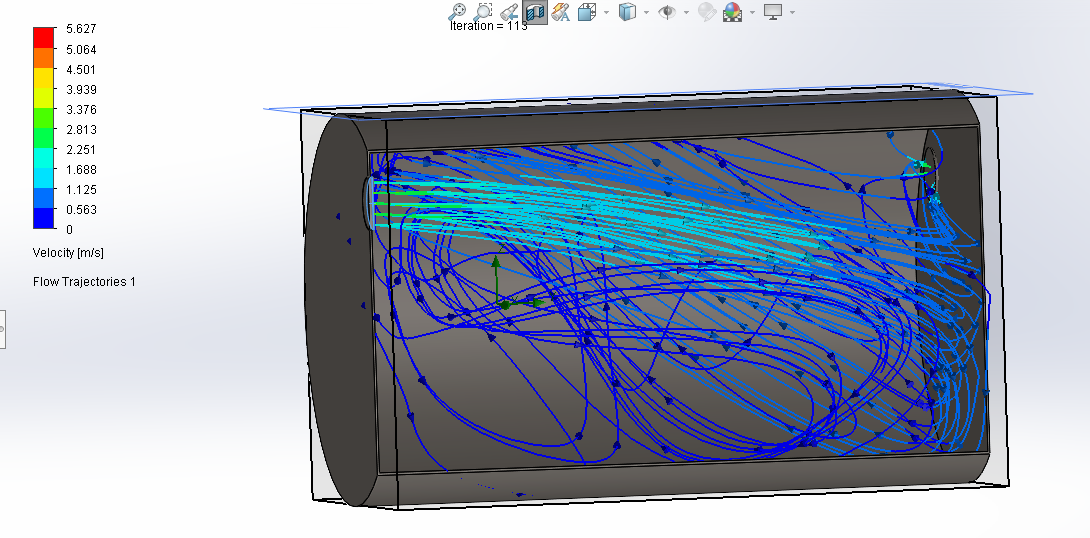
\includegraphics[scale=0.4]{images/Capitulo 4/s5/Contenedor/flow2.png}
            \caption{Configuración de ventiladores en caras laterales opuestas}
            \label{fg:ventilador_co}
     \end{figure}

Para la última configuración se propuso hacer llegar el aire directamente a la mezcla por medio de un tubo introducido por la parte superior del contenedor, llegando unos centimetros arriba del nivel de la mezcla, lo que provocaría la inyección de aire en la parte inferior del tambo. Esta configuración aparente ser muy buena ya que el aire frío por su densidad se localizaría en la parte inferior del contenedor y una vez que el aire se caliente, este ascendería gradualmente y sería expulsado por el otro ventilador, sin embargo se debe tener en cuenta que requerirá de un mayor trabajo de manufactura.

        \begin{figure}[h!]
            \centering
            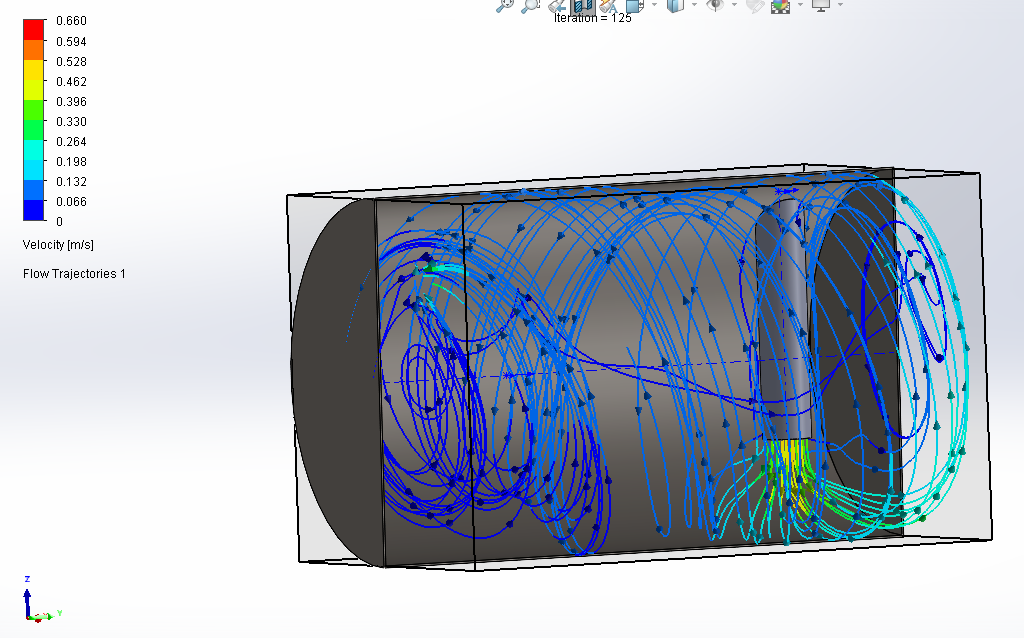
\includegraphics[scale=0.4]{images/Capitulo 4/s5/Contenedor/Flow_Profe_Islas.png}
            \caption{Configuración de ventiladores, aire inyectado directamente en la mezcla }
            \label{fg:ventilador_cilindro}
     \end{figure}


 Como se pudo observar, las distribuciones que mejor se acoplan a lo requerido, serían la primera \ref{fg:ventilador_mcara} y la tercera configuración \ref{fg:ventilador_cilindro}. Y aunque la última propuesta podría tener el mejor comportamiento de las tres, presenta un riesgo en su manufactura pues se requiere la incorporación del cilindro que llevará el aire al interior del contenedor, necesitará de un buen sellado en la parte superior y existe la posibilidad de que el contenedor se dañe quedando inservible, es importante mencionar que el tambo será uno de los componentes más costosos del proyecto por lo que no sería viable para el equipo. Por lo que estaría optando por utilizar la primer configuración, pues la colocación de los ventiladores en la cara lateral del tambo resulta más sencilla  y el riesgo de dañar el contenedor aparenta ser menor.
%\section{Código del sistema de compostaje}\label{Ap:Codigo_completo}

El código del sistema de compostaje, consta de la declaración de las librerías que se utilizan en el programa, también de la estructura de los hilos necesarios para su funcionamiento. El programa se realizo en la interfaz de Arduino, para la tarjeta NodeMCU-32S.

También cuenta con una rutina donde va almacenando el tiempo de operación y su modo de prueba, para probar cada uno de los sistemas de manera individual. 

\ArduinoSketch{Codigo_compost}{Código del sistema de compostaje}

\part{Anexos}
\anexo
%\chapter{Anexo 1. Placa del motor de aireación}\label{anexo1}
\stepcounter{chapter} %instrucción necesaria para cambiar numeración

Placa de especificaciones del motor utilizado en el proceso de aireación, en este caso se trata de un motor de corriente alterna a 1/4 de caballo de fuerza.

 \begin{figure}[h!]
            \centering
            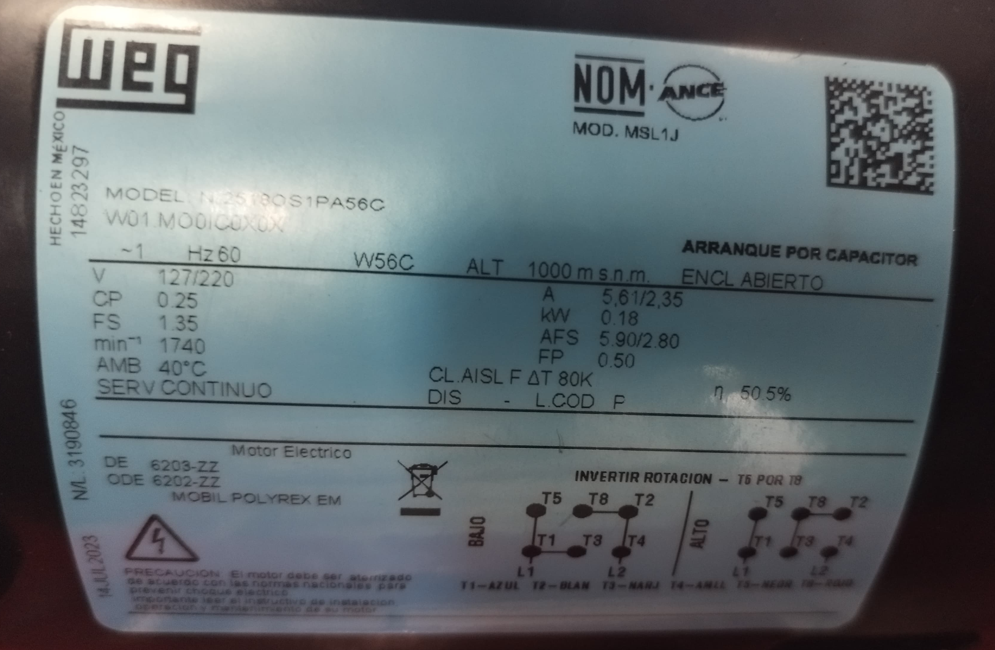
\includegraphics[scale=0.4]{images/Anexo/motor_air.png}
            \caption{Características del motor de aireación}
            \label{fg:motor_airo_esp}
 \end{figure}


\bigskip






%%%%%%fin del archivo
\endinput 
%\chapter{Anexo 2. Placa del motor de tituración}\label{anexo2}
\stepcounter{chapter} %instrucción necesaria para cambiar numeración

Placa con los datos técnicos del motor utilizado en la etapa de trituración. Este fue un motor de lavadora Koblenz de 16 Kg.

 \begin{figure}[h!]
            \centering
            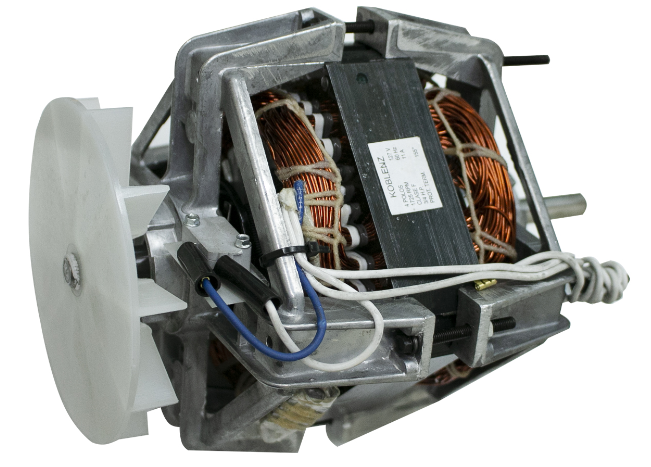
\includegraphics[scale=0.5]{images/Anexo/motor_lav.png}
            \caption{Motor de Lavadora Koblenz de 16 Kg}
            \label{fg:motor_imagen_lavadora}
 \end{figure}

  \begin{figure}[h!]
            \centering
            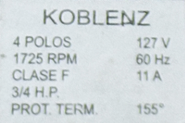
\includegraphics[scale=1]{images/Anexo/motor_lav_esp.png}
            \caption{Especificaciones del motor de lavadora Koblenz}
            \label{fg:motor_lav_esp}
 \end{figure}





\bigskip



%%%%%%fin del archivo
\endinput 
%\include{apendices/anexo3}
\newpage
%%%%%%%%%%%%%%%%%%%%%%%%%%%%%%%%%%%%%%%%%%%%%%%%%%%%%%%%%%%%%%%%%%%%%%%
%%%%%%%%%%%%%%%%%%%%%%%%%%%%  INDICE ALFABÉTICO%%%%%%%%%%
\IndiceAlfabetico
\end{document}
%%%%%%%%%%%%%%%%%%%%%%%%%%%%%%%%%%%%%%%%%%%%%%%%%%%%%%%%%%%%%%%%%%%%%%%%%%%%%%%%%% 